% Options for packages loaded elsewhere
\PassOptionsToPackage{unicode}{hyperref}
\PassOptionsToPackage{hyphens}{url}
\PassOptionsToPackage{dvipsnames,svgnames,x11names}{xcolor}
%
\documentclass[
]{book}
\usepackage{amsmath,amssymb}
\usepackage{iftex}
\ifPDFTeX
  \usepackage[T1]{fontenc}
  \usepackage[utf8]{inputenc}
  \usepackage{textcomp} % provide euro and other symbols
\else % if luatex or xetex
  \usepackage{unicode-math} % this also loads fontspec
  \defaultfontfeatures{Scale=MatchLowercase}
  \defaultfontfeatures[\rmfamily]{Ligatures=TeX,Scale=1}
\fi
\usepackage{lmodern}
\ifPDFTeX\else
  % xetex/luatex font selection
\fi
% Use upquote if available, for straight quotes in verbatim environments
\IfFileExists{upquote.sty}{\usepackage{upquote}}{}
\IfFileExists{microtype.sty}{% use microtype if available
  \usepackage[]{microtype}
  \UseMicrotypeSet[protrusion]{basicmath} % disable protrusion for tt fonts
}{}
\makeatletter
\@ifundefined{KOMAClassName}{% if non-KOMA class
  \IfFileExists{parskip.sty}{%
    \usepackage{parskip}
  }{% else
    \setlength{\parindent}{0pt}
    \setlength{\parskip}{6pt plus 2pt minus 1pt}}
}{% if KOMA class
  \KOMAoptions{parskip=half}}
\makeatother
\usepackage{xcolor}
\usepackage{color}
\usepackage{fancyvrb}
\newcommand{\VerbBar}{|}
\newcommand{\VERB}{\Verb[commandchars=\\\{\}]}
\DefineVerbatimEnvironment{Highlighting}{Verbatim}{commandchars=\\\{\}}
% Add ',fontsize=\small' for more characters per line
\usepackage{framed}
\definecolor{shadecolor}{RGB}{248,248,248}
\newenvironment{Shaded}{\begin{snugshade}}{\end{snugshade}}
\newcommand{\AlertTok}[1]{\textcolor[rgb]{0.94,0.16,0.16}{#1}}
\newcommand{\AnnotationTok}[1]{\textcolor[rgb]{0.56,0.35,0.01}{\textbf{\textit{#1}}}}
\newcommand{\AttributeTok}[1]{\textcolor[rgb]{0.13,0.29,0.53}{#1}}
\newcommand{\BaseNTok}[1]{\textcolor[rgb]{0.00,0.00,0.81}{#1}}
\newcommand{\BuiltInTok}[1]{#1}
\newcommand{\CharTok}[1]{\textcolor[rgb]{0.31,0.60,0.02}{#1}}
\newcommand{\CommentTok}[1]{\textcolor[rgb]{0.56,0.35,0.01}{\textit{#1}}}
\newcommand{\CommentVarTok}[1]{\textcolor[rgb]{0.56,0.35,0.01}{\textbf{\textit{#1}}}}
\newcommand{\ConstantTok}[1]{\textcolor[rgb]{0.56,0.35,0.01}{#1}}
\newcommand{\ControlFlowTok}[1]{\textcolor[rgb]{0.13,0.29,0.53}{\textbf{#1}}}
\newcommand{\DataTypeTok}[1]{\textcolor[rgb]{0.13,0.29,0.53}{#1}}
\newcommand{\DecValTok}[1]{\textcolor[rgb]{0.00,0.00,0.81}{#1}}
\newcommand{\DocumentationTok}[1]{\textcolor[rgb]{0.56,0.35,0.01}{\textbf{\textit{#1}}}}
\newcommand{\ErrorTok}[1]{\textcolor[rgb]{0.64,0.00,0.00}{\textbf{#1}}}
\newcommand{\ExtensionTok}[1]{#1}
\newcommand{\FloatTok}[1]{\textcolor[rgb]{0.00,0.00,0.81}{#1}}
\newcommand{\FunctionTok}[1]{\textcolor[rgb]{0.13,0.29,0.53}{\textbf{#1}}}
\newcommand{\ImportTok}[1]{#1}
\newcommand{\InformationTok}[1]{\textcolor[rgb]{0.56,0.35,0.01}{\textbf{\textit{#1}}}}
\newcommand{\KeywordTok}[1]{\textcolor[rgb]{0.13,0.29,0.53}{\textbf{#1}}}
\newcommand{\NormalTok}[1]{#1}
\newcommand{\OperatorTok}[1]{\textcolor[rgb]{0.81,0.36,0.00}{\textbf{#1}}}
\newcommand{\OtherTok}[1]{\textcolor[rgb]{0.56,0.35,0.01}{#1}}
\newcommand{\PreprocessorTok}[1]{\textcolor[rgb]{0.56,0.35,0.01}{\textit{#1}}}
\newcommand{\RegionMarkerTok}[1]{#1}
\newcommand{\SpecialCharTok}[1]{\textcolor[rgb]{0.81,0.36,0.00}{\textbf{#1}}}
\newcommand{\SpecialStringTok}[1]{\textcolor[rgb]{0.31,0.60,0.02}{#1}}
\newcommand{\StringTok}[1]{\textcolor[rgb]{0.31,0.60,0.02}{#1}}
\newcommand{\VariableTok}[1]{\textcolor[rgb]{0.00,0.00,0.00}{#1}}
\newcommand{\VerbatimStringTok}[1]{\textcolor[rgb]{0.31,0.60,0.02}{#1}}
\newcommand{\WarningTok}[1]{\textcolor[rgb]{0.56,0.35,0.01}{\textbf{\textit{#1}}}}
\usepackage{longtable,booktabs,array}
\usepackage{calc} % for calculating minipage widths
% Correct order of tables after \paragraph or \subparagraph
\usepackage{etoolbox}
\makeatletter
\patchcmd\longtable{\par}{\if@noskipsec\mbox{}\fi\par}{}{}
\makeatother
% Allow footnotes in longtable head/foot
\IfFileExists{footnotehyper.sty}{\usepackage{footnotehyper}}{\usepackage{footnote}}
\makesavenoteenv{longtable}
\usepackage{graphicx}
\makeatletter
\newsavebox\pandoc@box
\newcommand*\pandocbounded[1]{% scales image to fit in text height/width
  \sbox\pandoc@box{#1}%
  \Gscale@div\@tempa{\textheight}{\dimexpr\ht\pandoc@box+\dp\pandoc@box\relax}%
  \Gscale@div\@tempb{\linewidth}{\wd\pandoc@box}%
  \ifdim\@tempb\p@<\@tempa\p@\let\@tempa\@tempb\fi% select the smaller of both
  \ifdim\@tempa\p@<\p@\scalebox{\@tempa}{\usebox\pandoc@box}%
  \else\usebox{\pandoc@box}%
  \fi%
}
% Set default figure placement to htbp
\def\fps@figure{htbp}
\makeatother
\setlength{\emergencystretch}{3em} % prevent overfull lines
\providecommand{\tightlist}{%
  \setlength{\itemsep}{0pt}\setlength{\parskip}{0pt}}
\setcounter{secnumdepth}{5}
\usepackage{booktabs}
\usepackage{amsthm}
\makeatletter
\def\thm@space@setup{%
  \thm@preskip=8pt plus 2pt minus 4pt
  \thm@postskip=\thm@preskip
}

\makeatother
\ifxetex
\usepackage{polyglossia}
\setmainlanguage{spanish}
\renewcommand{\linethickness}{0.05em} % to fix linethickness pandoc issue

% para poner cover page en la version pdf
\usepackage{pdfpages}
\let\oldmaketitle\maketitle
\renewcommand{\maketitle}{
  
\includepdf{imagenes/cover.pdf}
}

% para tener bibliografia en el index
\usepackage[nottoc]{tocbibind}

% Tabla en lugar de cuadro
\gappto\captionsspanish{\renewcommand{\tablename}{Tabla}  
  \renewcommand{\listtablename}{Índice de tablas}}
\else
  \usepackage[spanish,es-tabla]{babel}
\fi

% For kableExtra
\usepackage{booktabs}
\usepackage{longtable}
\usepackage{array}
\usepackage{multirow}
\usepackage{wrapfig}
\usepackage{float}
\usepackage{colortbl}
\usepackage{pdflscape}
\usepackage{tabu}
\usepackage{threeparttable}
\usepackage{threeparttablex}
\usepackage[normalem]{ulem}
\usepackage{makecell}
\usepackage{xcolor}
\usepackage{booktabs}
\usepackage{longtable}
\usepackage{array}
\usepackage{multirow}
\usepackage{wrapfig}
\usepackage{float}
\usepackage{colortbl}
\usepackage{pdflscape}
\usepackage{tabu}
\usepackage{threeparttable}
\usepackage{threeparttablex}
\usepackage[normalem]{ulem}
\usepackage{makecell}
\usepackage{xcolor}
\usepackage[]{natbib}
\bibliographystyle{apalike}
\usepackage{bookmark}
\IfFileExists{xurl.sty}{\usepackage{xurl}}{} % add URL line breaks if available
\urlstyle{same}
\hypersetup{
  pdftitle={Un Recorrido por los Métodos Cuantitativos en Ciencias Sociales a bordo de R},
  pdfauthor={Eduardo Bologna},
  colorlinks=true,
  linkcolor={Maroon},
  filecolor={Maroon},
  citecolor={Blue},
  urlcolor={Blue},
  pdfcreator={LaTeX via pandoc}}

\title{Un Recorrido por los Métodos Cuantitativos en Ciencias Sociales a bordo de R}
\author{Eduardo Bologna}
\date{27 julio, 2025}

\begin{document}
\maketitle

{
\hypersetup{linkcolor=}
\setcounter{tocdepth}{1}
\tableofcontents
}
\begin{center}\rule{0.5\linewidth}{0.5pt}\end{center}

\chapter*{Colaboradores}\label{colaboradores}
\addcontentsline{toc}{chapter}{Colaboradores}

\subsection*{Comité Editorial}\label{comituxe9-editorial}
\addcontentsline{toc}{subsection}{Comité Editorial}

\subsubsection*{Patricia Caro}\label{patricia-caro}
\addcontentsline{toc}{subsubsection}{Patricia Caro}

\subsubsection*{Marcos Cupani}\label{marcos-cupani}
\addcontentsline{toc}{subsubsection}{Marcos Cupani}

\subsubsection*{Adriana D´Amelio}\label{adriana-damelio}
\addcontentsline{toc}{subsubsection}{Adriana D´Amelio}

\subsubsection*{Maria Silvia Galibert}\label{maria-silvia-galibert}
\addcontentsline{toc}{subsubsection}{Maria Silvia Galibert}

\subsubsection*{Jorge Lorenzo}\label{jorge-lorenzo}
\addcontentsline{toc}{subsubsection}{Jorge Lorenzo}

\subsubsection*{María Marta Santillan}\label{maruxeda-marta-santillan}
\addcontentsline{toc}{subsubsection}{María Marta Santillan}

\begin{center}\rule{0.5\linewidth}{0.5pt}\end{center}

\subsection*{Edición en bookdown}\label{ediciuxf3n-en-bookdown}
\addcontentsline{toc}{subsection}{Edición en bookdown}

\subsubsection*{\texorpdfstring{\href{https://jcrodriguez.rbind.io/}{Juan Cruz Rodriguez}}{Juan Cruz Rodriguez}}\label{juan-cruz-rodriguez}
\addcontentsline{toc}{subsubsection}{\href{https://jcrodriguez.rbind.io/}{Juan Cruz Rodriguez}}

\begin{center}\rule{0.5\linewidth}{0.5pt}\end{center}

\subsection*{Revisión de lenguaje incluyente}\label{revisiuxf3n-de-lenguaje-incluyente}
\addcontentsline{toc}{subsection}{Revisión de lenguaje incluyente}

\subsubsection*{Melody del Rio}\label{melody-del-rio}
\addcontentsline{toc}{subsubsection}{Melody del Rio}

\chapter*{Presentación}\label{presentaciuxf3n}
\addcontentsline{toc}{chapter}{Presentación}

Este manual toma como punto de partida nuestro trabajo anterior \emph{Métodos Estadísticos de Investigación} \citep{bologna2018}. En lo didáctico, los cambios provienen de la experiencia acumulada luego de diez años de uso en carreras de Ciencias Sociales y Humanas de grado y posgrado. Los contenidos se han ajustado tomando en consideración el uso que se hace actualmente de la estadística en investigación social.

El respeto al uso de lenguaje incluyente ha tenido en cuenta la discusión actual en la Universidad Nacional de Córdoba y las sugerencias para la Separata del Manual de Estilo (en proceso de redacción, según RHCS-2019-1094-E-UNC-REC), que busca superar los usos sexistas, sin abandonar las reglas del sistema de la lengua castellana. Por razones técnicas, se ha debido apelar al uso de la letra \emph{e} en reemplazo del masculino o femenino, en los nombres de variables o de matrices de datos.\\
En consideración al criterio de Ciencia Abierta, las bases y los scripts usados en el manual están disponibles en \url{https://github.com/jcrodriguez1989/EstadisticaParaCienciasSocialesConR}, por lo que es posible reproducir los ejemplos mostrados en el texto, a partir de los datos originales. Además, el manual está abierto al aporte de sugerencias por parte de lectores o docentes que opten por referenciarlo (enviando las sugerencias al repositorio de GitHub).

Los temas que el manual recorre se presentan a partir de nociones básicas, para ilustrar la continuidad que hay entre las formas corrientes de razonar y su formalización. Se pone el acento en tres aspectos del uso de las técnicas: i) la comprensión del razonamiento que las sostiene, ii) los supuestos que autorizan su uso, y iii) la lectura e interpretación de los resultados. Al final del curso, se espera que quienes hayan recorrido de este manual puedan decidir ante qué interrogantes corresponde aplicar cada procedimiento, bajo qué condiciones se puede apelar a él y cómo se lee el resultado. Así es como se usa la estadística en el desempeño profesional o en investigación. El software elegido para aplicar las técnicas es R \citep{R} en entorno RStudio \citep{RStudioTeam2018}, por un conjunto de razones que se explicitan más adelante.

Las aplicaciones informáticas, que implican el modo de solicitar a R las operaciones de análisis están separadas de la discusión sobre contenidos y procedimientos, se decidió así por dos razones. La primera es que el manual puede ser usado en cursos que no incluyan las aplicaciones informáticas, sino que los objetivos se limiten a la comprensión e interpretación de procedimientos estadísticos, mientras que otros cursos pueden tener interés en el ``cómo hacerlo'', y necesitan algunas instrucciones para tener un manejo inicial de R. La segunda razón es que la elección de software de análisis de datos, del ``paquete estadístico'', suele depender de preferencias del equipo docente y así el manual no queda atado exclusivamente a R.

Las fórmulas se consideran como una manera compacta de expresar relaciones entre conceptos y su uso para el cálculo está limitado, debido a que en la actualidad, las operaciones matemáticas se solicitan a paquetes informáticos especializados. Cada técnica que se describe tiene un fundamento teórico cuyo contenido matemático excede el interés de la mayoría de potenciales usuarias y usuarios de este manual. Sin embargo, para interpretar adecuadamente un resultado o para decidir si determinada técnica puede aplicarse, es necesario conocer esos fundamentos; hemos intentado presentarlos apelando en la menor medida posible a conocimientos matemáticos previos y usando un mínimo de formalización.

El manual está organizado en tres partes que articulan los dos conjuntos de procedimientos por medio de los cuales la Estadística aporta a la construcción de conocimiento: el resumen de un conjunto grande de información y la extensión de las conclusiones que se observan en ciertos casos, a otros casos que no han sido observados. Estos dos conjuntos se denominan Estadística Descriptiva y Estadística Inferencial respectivamente. Las partes I y III de este manual corresponden a cada uno de ellos, mientras que la parte II es de transición, entre la certeza de la descripción de datos observados y la incertidumbre que acompaña a la generalización.

\section*{Recorridos posibles}\label{recorridos-posibles}
\addcontentsline{toc}{section}{Recorridos posibles}

\begin{itemize}
\item
  La parte I tiene suficiente autonomía como para constituir en sí misma, material bibliográfico para un curso de estadística descriptiva.
\item
  La parte III contiene lo inferencial, y requiere una introducción al concepto de probabilidad y de variabilidad muestral. Puede usarse la parte II como esta introducción o, según la naturaleza del curso, ésta puede presentarse de manera abreviada.
\item
  Cada capítulo termina con un apartado llamado ``Hacerlo en R'' que muestra como pedir a R las operaciones que se han visto en ese capítulo. Estos apartados puede ser obviados en los cursos que no incluyan las aplicaciones informáticas entre sus objetivos, o bien reemplazados por otros, según el software de análisis de datos que se elija.
\end{itemize}

\chapter*{Introducción}\label{introducciuxf3n}
\addcontentsline{toc}{chapter}{Introducción}

Los procesos que involucran humanos, sean sociales, psicológicos, políticos, educativos, se caracterizan por su complejidad; es imposible predecir un resultado a partir del conocimiento de condiciones iniciales. Resultados electorales, reacciones de una persona en una situación dada, derroteros que sigue una protesta colectiva, a menudo discurren de modos que llamamos ``impensados'', haber conocido ciertos aspectos de estos procesos con antelación no nos habría permitido anticipar su devenir de manera exacta. Esto nos aleja de la ilusión determinística, o al menos de nuestra posibilidad de conocer una eventual determinación. Pero este rechazo al determinismo, no implica indeterminación. No es cierto que estemos en estado de ignorancia completa frente a la anticipación de procesos humanos, por el contrario, lo que tenemos es conocimiento parcial sobre algunos elementos que facilitan o hacen menos factibles ciertas consecuencias. Podemos aspirar a un conocimiento aproximado: entre el determinismo y la indeterminación, nuestro conocimiento se construye identificando condiciones bajo las cuales algunos hechos o procesos son más probables que otros. La manera formal de hacerlo es descomponiendo la diversidad en una parte que podemos explicar y otra que está fuera de nuestro alcance, llamamos variabilidad explicada a la primera y variabilidad aleatoria a la otra. La Estadística provee herramientas para trabajar con una forma de hacer investigación: el enfoque cuantitativo, que formula hipótesis sobre las explicaciones de hechos, fenómenos o procesos, observados y analiza cuán plausibles son, a la luz de los hechos. No permite alcanzar explicaciones completas, éstas siempre estarán afectadas por una componente de incertidumbre, propia de los procesos que involucran a seres humanos.

El cuantitativo no es el único enfoque que sirve para construir conocimiento validado y tampoco es incompatible con otras maneras de enfrentar la diversidad que nos rodea. Toda disciplina científica debe superar las creencias de ``sentido común'', esta ilusión de conocer, pero especialmente importante es eliminar los prejuicios en el campo de las ciencias que tratan con sujetos humanos, porque es allí donde más abundan y más daño pueden causar. Expresiones como ``Esta persona es así porque de chica no la tenían en cuenta'', ``No tiene dotes para la matemática'', ``Los sueños anuncian lo que va a pasar''; ``Las mujeres tienen más sensibilidad que los hombres'', ``El electorado premia o castiga con el voto la gestión de gobierno'', son, en el mejor de los casos, parciales y en el peor, falsas, provienen de creencias, de tradiciones, de voces populares transmitidas de una generación a la siguiente. La Estadística aporta a la investigación y con ella al descubrimiento de relaciones entre hechos, y a fundamentar esos descubrimientos. Lo hace con una mirada aguda y acotada, una mirada, que no aspira a ofrecer un conocimiento sobre alguna totalidad, sino sobre aspectos parciales del mundo que nos rodea. En esa limitación yace su fortaleza para poner en crisis la ilusión de conocer, en particular en Ciencias Sociales, donde lo que observamos nos atañe de manera muy próxima, y no es raro confundir ``lo que sucede'' con lo que creemos, opinamos o suponemos sobre ello.

La presencia de Estadística en carreras de Ciencias Sociales, Humanas y de la Salud se justifica en primer lugar en que a menudo la investigación empírica usa información proveniente de colectivos, y se dispone de datos que requieren que se los resuma para poder interpretarlos, una vez obtenidas conclusiones acerca de esos casos que han sido observados, suele buscarse generalizar los resultados a otros casos, que no se observaron. Ambas operaciones ―resumir y generalizar―, requieren de la Estadística.

En segundo lugar, en las carreras de grado y posgrado de esas disciplinas hay varias materias que requieren que se conozca estadística básica para comprender los resultados de investigaciones que son material de estudio. Muy a menudo, esos resultados se expresan en lenguaje estadístico y se mencionan técnicas de análisis que deben conocerse para poder hacer críticas.

En tercer lugar, quienes se dediquen al ejercicio profesional aplicarán técnicas de intervención y de análisis en sus distintos campos de especialización, y estas técnicas están basadas en la teoría y en el estado del conocimiento en un momento dado. Así como luego de un tiempo de haber usado una droga puede descubrirse que no produce los efectos deseados, también vale esto para cualquier intervención profesional: una terapia, una estrategia didáctica, una recomendación de política pública, un asesoramiento de campaña política. La idea según la cual el conocimiento científico es revisable, se refiere a que en cualquier momento puede hallarse nueva evidencia que contradiga las convicciones presentes. Por cierto, no se trata de cualquier evidencia, sino de la que proviene de procedimientos cuidadosos de observación, registro, comparación, medición y análisis; en pocas palabras, de la investigación. Lo que sabemos y lo que aprendamos para desempeñarnos como profesionales es el conocimiento de que se dispone en este momento, y que está en continua reelaboración a través de la investigación. Una vez que quienes hoy están estudiando en la universidad terminen sus carreras y trabajen como profesionales, asistirán a cambios en el modo de intervenir, nuevos enfoques terapéuticos, formas de tratar con grupos, estrategias didácticas, modos de análisis de las desigualdades. Eso no se aprenderá en la Facultad, se aprenderá luego, manteniéndose actualizado, leyendo revistas científicas, asistiendo a congresos; en fin enterándose de cómo cambia el conocimiento y se revisan los saberes a partir de los resultados de la investigación. Y la investigación usa la estadística muy a menudo. Si no se puede leer un artículo científico porque no se entiende lo que dicen las cifras, solo se podrá tener una idea superficial del resultado, más grave aún; quien decida que solo leerá la información que no contenga cifras, se quedará con una pequeña parte de todo lo que se publica.

Esa limitación puede ser peligrosa: si no se entiende cómo se obtuvieron determinados resultados, no se los puede cuestionar, dudar de ellos, discutir procedimientos, porque parecerán ajenos.

La Estadística tiene rol importante en la construcción, validación e interpretación de resultados de instrumentos de medición: tests de inteligencia, de desarrollo, escalas de actitudes, de preferencias, de opinión, de valores.

Por último, y aunque no parezca obvio, la Estadística nos sirve en la vida diaria. El ejercicio de nuestros derechos ciudadanos necesita que podamos darnos cuenta de lo que nos dicen las mediciones de audiencia, las consultoras políticas, los laboratorios de medicamentos, los indicadores nutricionales de lo que comemos, las estadísticas oficiales (nivel de desempleo, pobreza, inflación), entre otras fuentes de información. ¿A quiénes consultaron para decidir que un programa de televisión se levanta y otro se sostiene? ¿Cómo se hacen las encuestas que indican quién va a ganar las elecciones? ¿Qué implica que una técnica anticonceptiva sea eficaz en el 99\% de los casos? Somos nosotras/os quienes vemos la programación que se ofrece, quienes sufrimos los resultados de una elección de autoridades, quienes consumimos. Mucha de esa información usa estadísticas y hay parte del vocabulario que no es comprensible para todo el mundo pero que, por habernos habituado a escuchar, creemos conocer, ya que las palabras nos suenan familiares: el promedio, un porcentaje, que una diferencia sea significativa. Cada una de esas expresiones tiene un significado preciso; si no lo conocemos no podemos cuestionar las decisiones.

Que no lo conozcamos, que muchos prefieran no conocerlo y que haya quienes operan para que la Matemática -y por extensión la Estadística-, sean de difícil acceso a los estudiantes, no es por azar, es funcional a un modo de producción que requiere que requiere que gran parte de la sociedad sea silenciada con argumentos que usan terminología críptica. Por esto, nuestra aspiración no se limita a transmitir un conjunto de técnicas de análisis de datos, sino a proveer herramientas que ayuden a mirar al mundo desde una posición más informada, y esperamos que eso implique también una posición más crítica y hasta quizás transformadora, que pueda poner en duda certezas establecidas.

\chapter*{Antes de empezar}\label{antes-de-empezar}
\addcontentsline{toc}{chapter}{Antes de empezar}

\section*{Materiales}\label{materiales}
\addcontentsline{toc}{section}{Materiales}

A lo largo del manual se usan datos para ejemplificar procedimientos. Algunos de ellos son ficticios y han sido construidos especialmente para ilustrar algún aspecto de una distribución o del resultado de una técnica. Sin embargo, la mayoría de los ejemplos están realizados a partir de datos reales, provenientes de bases de datos de libre disponibilidad que hemos elegido teniendo en cuenta los intereses de los púbicos a que nos dirigimos. Estas bases son las que se presentan a continuación, en el repositorio \url{https://github.com/jcrodriguez1989/EstadisticaParaCienciasSocialesConR} se encuentra una descripción más detallada, así como los cuestionarios, las bases de datos correspondientes y los manuales de códigos para poner en correspondencia los nombres de las variables dados en la base, con los aspectos que se indagan de las unidades (hogares o personas).

\subsection*{Encuesta Permanente de Hogares}\label{encuesta-permanente-de-hogares}
\addcontentsline{toc}{subsection}{Encuesta Permanente de Hogares}

La EPH es un programa nacional de producción permanente de indicadores sociales cuyo objetivo es conocer las características socioeconómicas de la población. Es realizada en forma conjunta por el Instituto Nacional de Estadística y Censos (INDEC) y las Direcciones Provinciales de EstadÌstica (DPE) \citep{INDEC2003}. Los datos se recogen por medio de dos cuestionarios; uno de ellos que pregunta por características del hogar y la vivienda y el otro por las personas individualmente.

\subsection*{Encuesta Nacional de Factores de Riesgo}\label{encuesta-nacional-de-factores-de-riesgo}
\addcontentsline{toc}{subsection}{Encuesta Nacional de Factores de Riesgo}

La tercera ENFR es un estudio de corte transversal que permite vigilar la prevalencia de factores de riesgo de enfermedades no transmisibles y evaluar su evolución en comparación con las ediciones anteriores realizadas en los años 2005 y 2009. Es realizada conjuntamente entre el Instituto Nacional de Estadística y Censos (INDEC) y el Ministerio de Salud de la Nación de la República Argentina.

La encuesta tiene por objetivos: Conocer la distribución de los factores de riesgo en la población de 18 años y más. Estimar su prevalencia. Determinar el perfil de la población bajo riesgo a través de sus características sociodemográficas, socioeconómicas, educativas y del entorno familiar social \citep{msal2013, INDEC2013a}.

\subsection*{Latinobarómetro}\label{latinobaruxf3metro}
\addcontentsline{toc}{subsection}{Latinobarómetro}

Latinobarómetro es un estudio de opinión pública que aplica anualmente alrededor de 20.000 entrevistas en 18 países de América Latina representando a más de 600 millones de habitantes.

Corporación Latinobarómetro es una ONG sin fines de lucro con sede en Santiago de Chile, única responsable de la producción y publicación de los datos.

La Corporación Latinobarómetro investiga el desarrollo de la democracia, la economía y la sociedad en su conjunto, usando indicadores de opinión pública que miden actitudes, valores y comportamientos. Los resultados son utilizados por los actores socio políticos de la región, actores internacionales, gubernamentales y medios de comunicación \citet{Latinobarometro2010}, \citet{Latinobarometro2019}.

\subsection*{Encuesta Nacional sobre Prevalencias de Consumo de Sustancias Psicoactivas}\label{encuesta-nacional-sobre-prevalencias-de-consumo-de-sustancias-psicoactivas}
\addcontentsline{toc}{subsection}{Encuesta Nacional sobre Prevalencias de Consumo de Sustancias Psicoactivas}

La encuesta produce datos sobre:

• La cantidad de personas que declararon haber consumido sustancias psicoactivas en diferentes períodos de referencia (prevalencias) y su incidencia en relación con la población total. Las sustancias psicoactivas comprenden: las drogas legales o sociales (tabaco, bebidas alcohólicas), ilegales (marihuana, cocaína, pasta base, éxtasis, opiáceos y anestésicos, crack, alucinógenos, inhalables y otras drogas) y fármacos (estimulantes, tranquilizantes, anorexígenos);

• Las características sociodemográficas, socioeconómicas, educativas y del entorno familiar social de la población de 16 a 65 años de edad que consume sustancias psicoactivas.

El objetivo general de esta Encuesta fue contribuir a actualizar el sistema de información sobre el consumo de sustancias psicoactivas a nivel nacional y, de esa manera, al diseño de políticas públicas más eficaces, orientadas a mejorar las condiciones de salud de la población \citet{Indec2008}, \citet{La2008}.

\subsection*{Aplicación de la escala de Bayley}\label{aplicaciuxf3n-de-la-escala-de-bayley}
\addcontentsline{toc}{subsection}{Aplicación de la escala de Bayley}

La base provista contienen 454 casos de niñas y niños sometidos a evaluación por medio de las subescalas mental y motora de la escala de Bayley.\\
La Escala Bayley de Desarrollo Infantil se aplica en personas de los 2 a los 36 meses de vida y ha sido adaptada a Córdoba a las edades de 0 a 24 meses por \citet{Rodriguez2005}. Los dos primeros años de vida humana son momentos cruciales para inferir de manera temprana la evolución del desarrollo posterior \citep{papalia2004}.\\
La prueba, de origen norteamericano, consta de varias versiones desde su creación por su autora Nancy Bayley en 1933, existen revisiones de 1969, 1977 y 1993.
Las escalas de Bayley (EBDI) fueron publicadas en el año 1969. En España aparecieron estandarizadas en el año 1977, y la revisión americana (las Bayley Scale of Infant Development-II o BSID II) fueron publicadas en 1993, \citet{Albers2007}, \citet{Ballot2017}. El interés por disponer de unas escalas adecuadamente tipificadas como las Bayley creció a lo largo de la primera mitad del siglo XX, al ir aumentando el conocimiento de las capacidades infantiles, los cambios cerebrales durante la etapa posnatal y el estudio de cómo influyen los factores del medio, la familia y los individuos en el desarrollo temprano. Además, la proporción de personas prematuras ha ido aumentando considerablemente a lo largo de los años, con el consiguiente aumento de casos que nacen con el riesgo de presentar un retraso en el desarrollo.\\
El objetivo inicial de las escalas fue medir la inteligencia a edades muy tempranas. Los ítems que la componen están ordenados en una secuencia de dificultades que aumentan con la edad. En su forma actual, la EBDI permite medir el desarrollo mental, el desarrollo psicomotor y el comportamiento infantil.\\
El nivel de desarrollo mental tiene 163 ítems que miden el desarrollo por medio de una serie de habilidades. El nivel del desarrollo motor se compone de 81 ítems que representan tanto habilidades motoras finas como gruesas, y se centra principalmente en el grado de control del cuerpo y la coordinación de los movimientos. La distinción entre la escala mental y motora se justifica porque se parte de que la preplanificación y el razonamiento son componentes de las actividades mentales, pero no de las habilidades motoras. Por tanto, los ítems de las dos escalas son distintos, aunque en algunas ocasiones una misma habilidad este incluida en ambas escalas. El registro comportamental del sujeto complementa la información obtenida mediante las escalas mental y motora, proporciona una descripción del comportamiento infantil relativo al que se esperaría de cualquier persona que estuviera en el mismo estadio.
Se dice que la escala de Bayley es una escala ecléctica, es decir los ítems no están agrupados por áreas, factores o subescalas con puntuaciones determinadas para cada una de ellas. No obstante, las Bayley II intenta incluir ítems de las cinco áreas que la guía americana para la evaluación de los candidatos de servicios especiales requiere que sean evaluadas: desarrollo físico, cognitivo, lingüístico, psicosocial y autoayuda. Sin embargo continúa sin haber medidas para cada una de estas áreas calificadas.\\
Como se menciono anteriormente en 1993 se publicó una revisión de las escalas originales. Las Bayley II mantienen la misma estructura y objetivos que la anterior, pero introducen algunos cambios como resultado de los trabajos de investigación sobre el desarrollo infantil en los últimos años y para mejorar la adecuación de los datos y el material a la población infantil. Uno de los cambios importantes es que se amplía la edad de evaluación desde el 1º mes hasta los 42 meses. Además se han incorporado ítems cuyo estudio han demostrado tener una adecuada fiabilidad y validez; así los 163 ítems de la escala mental y los 81 de la escala motora de Bayley han pasado a ser 178 y 111 respectivamente en las Bayley II.\\
Actualmente se utiliza la versión correspondiente a 1993. Como su autora lo indica, el objetivo principal de esta prueba es diagnosticar demoras del desarrollo y planificar estrategias de intervención. Actualmente puede decirse que esta Escala constituye uno de los test más utilizados para evaluar el desarrollo neuroconductual durante los primeros meses de vida, sin embargo es poco utilizada como herramienta de diagnóstico en nuestro medio. La misma está formada por tres Sub-Escalas:

\begin{itemize}
\item
  Escala Mental: Evalúa memoria, habituación, resolución de problemas, conceptualización numérica temprana, generalización, clasificación, vocalizaciones, lenguaje y habilidades sociales. Es decir estima aspectos relacionados con el desarrollo cognitivo y la capacidad de comunicación.
\item
  Escala Motora: Evalúa el control de los músculos gruesos y finos del cuerpo. Esto incluye movimientos asociados con rodar, girar, encogerse y estirarse, sentarse, pararse, caminar, correr y saltar. Se evalúa también la manipulación motora fina implicada en la prensión, adecuado uso de elementos de escritura e imitación de movimientos de las manos. En definitiva, evalúa el grado de coordinación corporal, así como habilidades motrices finas en manos y dedos.
\item
  Escala Comportamental: Evalúa aspectos cualitativos de la situación de examen como atención/alerta, orientación/interacción hacia la tarea, regulación emocional y calidad del movimiento. De este modo permite analizar la naturaleza de las orientaciones sociales y objetivas hacia el entorno. La información de esta escala debe utilizarse para suplementar la información cuantitativa de las dos escalas anteriores.
\end{itemize}

El desarrollo infantil implica un proceso de continuos cambios, en el cual la persona va a experimentar diversas trasformaciones y progresos. Estos cambios no sólo se advierten en el plano motor e intelectual (esto es, en su capacidad para dominar movimientos y razonar), sino que además se pueden apreciar múltiples reorganizaciones en el plano emocional (su capacidad para sentir) y social (su capacidad para relacionarse con su entorno).\\
La adquisición de estas competencias variará en función de la madurez neurofisiológica, de las características individuales, y de la riqueza y calidad de los estímulos de su entorno. De allí, la importancia de este período, pues sentará la base para el desarrollo y crecimiento óptimos.

La escala asigna puntajes brutos en función de la cantidad de pruebas exitosamente pasadas para una determinada edad. Posteriormente, estos puntajes brutos son transformados en índices mentales o motores que permiten ubicar a la persona evaluada en un nivel de desarrollo normal, levemente retrasado, significativamente retrasado o, si supera el normal, acelerado, para su edad.
Cada índice de desarrollo mental (IDM) y motor (IDP), tiene una distribución con una media de 100 y una desviación estándar de 15. Un puntaje de 100 o más en cualquier escala indica el nivel promedio de performance en una edad dada. Puntajes de 85 y 115 corresponden a 1 DS por debajo y por encima de la media y puntajes de 70 y 130 a 2 DS. En una distribución normal 2/3 de las personas evaluadas obtiene puntajes entre 85 y 115, 95\% entre 70 y 130 y casi todas (99,9\%) entre 55 y 145 (3 DS a cada lado de la media).

\subsection*{Tercera edad}\label{tercera-edad}
\addcontentsline{toc}{subsection}{Tercera edad}

Son los datos provenientes de una encuesta realizada a 506 personas adultas mayores que participan de las actividades del Centro de Promoción del Adulto Mayor (CEPRAM, \url{http://cepram.org.ar/}). Se releva grado de satisfacción con los talleres a que asisten y variables de clasificación: sexo, edad, grupo conviviente, educación, etc.

\section*{Herramientas}\label{herramientas}
\addcontentsline{toc}{section}{Herramientas}

\subsection*{La elección de R}\label{la-elecciuxf3n-de-r}
\addcontentsline{toc}{subsection}{La elección de R}

Para realizar análisis de datos existen numerosos programas informáticos, que se ocupan de los procesos computacionales, de manera que quienes los usan solo deban decidir qué procedimiento aplicar, cuidar que se cumplan las condiciones que hacen válido al procedimiento (los supuestos) y realizar una lectura correcta y completa del resultado que se obtiene, sin involucrarse con las operaciones de cálculo. Estos programas o ``paquetes estadísticos'' reúnen en un entorno único las operaciones más frecuentemente usadas en investigación y análisis de datos y las ponen al alcance de un público no especializado. Algunos de uso muy común son SPSS, SAS, INFOSTAT, STATA, STATISTICAL, etc. De la larga lista de opciones disponibles, este manual usa un software que se llama R, elección que se fundamenta en que R es varias cosas al mismo tiempo:

Es un software para análisis de datos: lo usan profesionales de la estadística, analistas de datos e investigadores de diversas disciplinas para extraer significado de información cuantitativa, para hacer descripciones e inferencias, visualización de datos y modelización predictiva.

Es un lenguaje de programación orientado a objetos, diseñado por profesionales de la estadística y para el uso en investigación cuantitativa: el análisis se hace escribiendo sentencias en este lenguaje, que provee objetos, operadores y funciones que hacen muy intuitivo el proceso de explorar, modelar y visualizar datos.

Es un ambiente para el análisis estadístico: en R hay funciones para prácticamente todo tipo de transformación de datos, de modelización y de representaciones gráficas que pueda hacer falta.

Es un proyecto de código abierto: esto significa no solo que se lo puede descargar y usar gratis, sino que el código es abierto y cualquiera puede inspeccionar o modificar las rutinas. Como sucede con otros proyectos de código abierto, como Linux, R ha mejorado sus códigos tras varios años de ``muchos ojos mirando'' y aportando soluciones. También como otros proyectos de código abierto, R tiene interfaces abiertas, por lo que se integra fácilmente a otras aplicaciones y sistemas.

Es una comunidad: R fue inicialmente desarrollado por Robert Gentleman y Ross Ihaka \citep{Ross1996}, del Departamento de Estadística de la Universidad de Auckland, en 1993 y desde entonces el grupo que dirige el proyecto ha crecido y se ha difundido por el mundo. Además, miles de otras personas han contribuido con funcionalidades adicionales por medio del aporte de ``paquetes'' que utilizan los 2 millones de personas que lo utilizan. Como resultado, existe una intensa comunidad de usuarios y usuarias de R on-line, con muchos sitios que ofrecen recursos para principiantes y también para quienes tienen más experiencia. A esa comunidad se puede recurrir para consultas y para salvar dificultades, son muy activas y dispuestas a ayudar.

R integra programas llamados paquetes, que sirven para realizar análisis específicos. Los paquetes son rutinas que realizan conjuntos de operaciones especializadas, y una de las potencialidades de R es que especialistas de diferentes disciplinas pueden desarrollar paquetes para determinados tipos de análisis y ponerlos a disposición del resto de la comunidad. En la actualidad hay más de 10000 paquetes y el conjunto crece porque la comunidad R es muy activa y continuamente se hacen aportes.

Actualmente, los principales medios de comunicación usan R para expresar datos de manera gráfica.

No solo cuenta con los métodos estándar sino que, debido a que los principales avances en procedimientos estadísticos se realizan en R, las técnicas más actualizadas están usualmente primero disponibles en R, quienes desarrollan paquetes comerciales necesitan tiempo poner las actualizaciones al alcance de sus clientes, y ellos a menudo deben pagar por las actualizaciones.

Permite la reproducción de los análisis por parte de cualquiera que conozca el código que se aplicó, por lo que aporta una herramienta necesaria en los proyectos de ciencia abierta, en especial para la reproducibilidad de los resultados.

Si no se cuenta con R instalado, es posible crear una cuenta en RStudio cloud (\url{https://rstudio.cloud/}) y trabajar con todos los archivos disponibles en la nube, sin necesidad de instalar localmente el software.

Por estas razones, R es uno de los lenguajes de programación que más uso tiene y se está convirtiendo en la lingua franca del análisis de datos.

Como lenguaje, R tiene varias interfaces gráficas, que es el modo en que las personas puede interactuar con él. R es el motor y del mismo modo en que, para manejar un auto no hace falta saber cómo funciona el motor, también aquí será suficiente contar con un buen conjunto de comandos (volante, pedales\ldots) para hacer uso de la potencia de ese motor, la interface provee esos comandos. De las interfaces existentes, hemos elegido RStudio \citep{RStudioTeam2018} que es un entorno de desarrollo integrado (IDE) de R para facilitar la edición de código que ofrece diversas herramientas para hacer muy accesible el uso de R por parte de quienes no se dedican a la programación, sino que aplican procedimientos estadísticos para sus trabajos de investigación.\\
Una línea de tiempo sobre el desarrollo de R puede encontrar en \url{https://blog.revolutionanalytics.com/2017/10/updated-history-of-r.html}

\subsection*{Instalación de R y RStudio}\label{instalaciuxf3n-de-r-y-rstudio}
\addcontentsline{toc}{subsection}{Instalación de R y RStudio}

En \url{http://cran.r-project.org} ``Download R for {[}Linux, Mac o Windows{]}'', y luego ``install R for the first time''. Una vez descargado, se instala siguiendo las instrucciones de las pantallas, aceptando las opciones por defecto que se ofrecen.

Una vez que R está instalado, se debe sumar RStudio. El lugar de descarga es \url{http://www.rstudio.com/products/rstudio/download/}. Allí se elige la versión gratis (free version) de RStudio Desktop y se baja hasta encontrar el sistema operativo y la version que corresponda a nuestro equipo. Luego se ejecuta el instalador de RStudio y se eligen las opciones por defecto. Cuando esté ya instalado, se accede por medio de RStudio; si al instalar R se creó un acceso directo a R en el escritorio, se lo puede eliminar. Al abrir RStudio, R es detectado automáticamente y desde allí operaremos.

\subsection*{Los componentes de RStudio}\label{los-componentes-de-rstudio}
\addcontentsline{toc}{subsection}{Los componentes de RStudio}

Cuando abrimos RStudio, vamos a encontrar tres paneles, uno a la izquierda, más grande, y dos a la derecha. En ``file'' se solicita un nuevo script, que se abre a la izquierda y ahora quedan cuatro paneles:

\begin{figure}
\centering
\pandocbounded{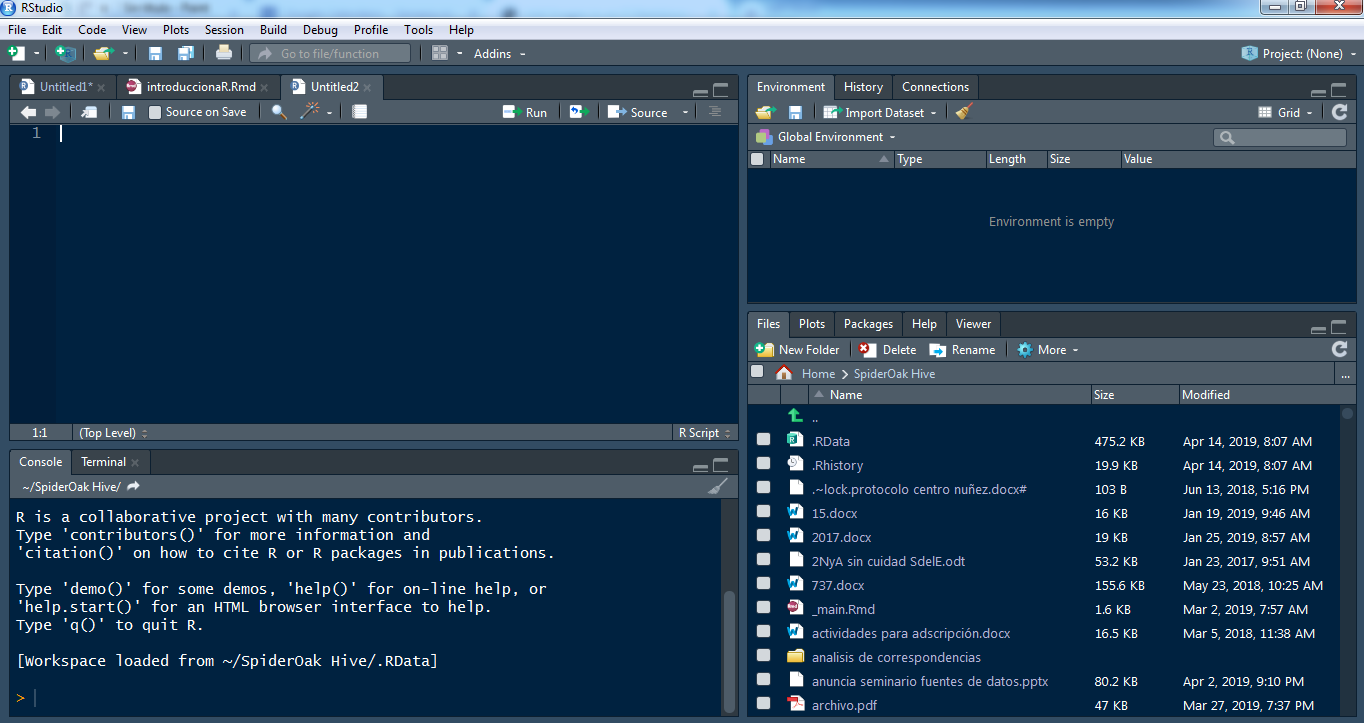
\includegraphics[keepaspectratio]{imagenes/entornoRStudio.png}}
\caption{Los cuatro paneles de RStudio}
\end{figure}

\begin{itemize}
\item
  Superior izquierdo es el script que se acaba de abrir, un documento editable en el que se escriben los comandos.
\item
  Inferior izquierdo es la consola, donde se encuentra la ejecución de los comandos y, si corresponde, los resultados de operaciones solicitadas.
\item
  Superior derecho es el entorno de trabajo, allí aparece cada uno de los objetos que se crean durante la sesión.
\item
  Inferior derecho, cuatro pestañas con los directorios de trabajo, los paquetes instalados, la ayuda (cuando se pide), los gráficos que se hagan.
\end{itemize}

\subsection*{Operaciones en el script}\label{operaciones-en-el-script}
\addcontentsline{toc}{subsection}{Operaciones en el script}

Antes de empezar a operar es necesario crear un lugar donde se alojarán los archivos que vamos a usar. Ese lugar, en R se llama ``proyecto''. Así, la primera acción será en File \rightarrow New Project \rightarrow New Directory \rightarrow New Project, darle un nombre y definir su ubicación en la computadora en que se trabaje. Si esa ubicación es una carpeta sincronizada (de drive o dropbox u otra) todos los archivos necesarios para trabajar en el proyecto estarán disponibles.

El script es un editor de textos en que se escriben comandos y se ejecutan, ya sea con el botón ``run'' o con una combinación de teclas que, según la configuración puede ser Ctrl+R o Ctrl+Enter. Una vez escrita la instrucción, se solicita su ejecución y se obtiene el resultado.\\
Los elementos que maneja R son objetos: un número, un vector, una base de datos, una tabla y muchos otros. Inicialmente, los que interesan a fin del análisis de datos son: vectores y matrices de datos.

\subsubsection*{Constante}\label{constante}
\addcontentsline{toc}{subsubsection}{Constante}

Un objeto numérico puede tener un valor fijo, si definimos a \textbf{x} como el número 3

\begin{Shaded}
\begin{Highlighting}[]
\NormalTok{x }\OtherTok{\textless{}{-}} \DecValTok{3}
\end{Highlighting}
\end{Shaded}

En el panel superior derecho aparece este objeto. El signo \textless- que define el objeto es equivalente a = que da la idea de asignar a \textbf{x} el valor 3.

Si se lo invoca (se lo llama es decir, se escribe su nombre), muestra su valor.

\begin{Shaded}
\begin{Highlighting}[]
\NormalTok{x}
\end{Highlighting}
\end{Shaded}

\begin{verbatim}
## [1] 3
\end{verbatim}

Las salidas de R, es decir los resultados que muestra, están antecedidos por un signo numeral (\#) y cada elemento de los resultados lleva su numeración entre corchetes. Aquí el resultado es solo un número, por eso hay un {[}1{]} a la izquierda.\\
Este objeto es un número, lo que puede saberse si se pregunta de qué clase es este objeto:

\begin{Shaded}
\begin{Highlighting}[]
\FunctionTok{class}\NormalTok{(x)}
\end{Highlighting}
\end{Shaded}

\begin{verbatim}
## [1] "numeric"
\end{verbatim}

Es numérico.

Si hubiésemos definido el objeto:

\begin{Shaded}
\begin{Highlighting}[]
\NormalTok{t }\OtherTok{\textless{}{-}} \StringTok{"a"}
\FunctionTok{class}\NormalTok{(t)}
\end{Highlighting}
\end{Shaded}

\begin{verbatim}
## [1] "character"
\end{verbatim}

Es carácter, para que lo acepte como valor nuevo, se debe poner entre comillas; de lo contrario, si se escribe:

\(t<-a\)

Buscará ese objeto, que no ha sido definido antes y dará error. Esta cualidad se puede usar cuando los números codifican categorías, como cuando se usa 1 para varones y 2 para mujeres:

\begin{Shaded}
\begin{Highlighting}[]
\NormalTok{u }\OtherTok{\textless{}{-}} \StringTok{"1"}
\FunctionTok{class}\NormalTok{(u)}
\end{Highlighting}
\end{Shaded}

\begin{verbatim}
## [1] "character"
\end{verbatim}

Allí se entiende al número como un código.

Otros tipos de objeto son lógicos

\begin{Shaded}
\begin{Highlighting}[]
\NormalTok{v }\OtherTok{\textless{}{-}} \ConstantTok{TRUE}
\FunctionTok{class}\NormalTok{(v)}
\end{Highlighting}
\end{Shaded}

\begin{verbatim}
## [1] "logical"
\end{verbatim}

El objeto \textbf{v} es lógico, esta clase de objeto puede tomar dos valores TRUE y FALSE.

Es posible transformar una clase de objeto en otra. Por ejemplo, si un valor numérico fue cargado como carácter, como el caso de \textbf{u} en el ejemplo anterior, se lo vuelve numérico pidiendo:

\begin{Shaded}
\begin{Highlighting}[]
\NormalTok{u }\OtherTok{\textless{}{-}} \FunctionTok{as.numeric}\NormalTok{(u)}
\FunctionTok{class}\NormalTok{(u)}
\end{Highlighting}
\end{Shaded}

\begin{verbatim}
## [1] "numeric"
\end{verbatim}

Pero si intentáramos eso con \textbf{t}, el resultado falla, porque no se interpreta un valor numérico.

Cuando el objeto es un número, se puede operar simplemente con él

\begin{Shaded}
\begin{Highlighting}[]
\DecValTok{5} \SpecialCharTok{*}\NormalTok{ x}
\end{Highlighting}
\end{Shaded}

\begin{verbatim}
## [1] 15
\end{verbatim}

Aquí no se creó ningún objeto nuevo, solo se hizo la operación y se mostró el resultado. Para crearlo, hace falta ponerle nombre:

\begin{Shaded}
\begin{Highlighting}[]
\NormalTok{y }\OtherTok{\textless{}{-}} \DecValTok{5} \SpecialCharTok{*}\NormalTok{ x}
\end{Highlighting}
\end{Shaded}

Y no veremos su valor hasta que no lo solicitemos

\begin{Shaded}
\begin{Highlighting}[]
\NormalTok{y}
\end{Highlighting}
\end{Shaded}

\begin{verbatim}
## [1] 15
\end{verbatim}

Suma resta, multiplicación y división se hacen con los signos que conocemos:

\begin{Shaded}
\begin{Highlighting}[]
\NormalTok{x }\SpecialCharTok{+}\NormalTok{ y}
\end{Highlighting}
\end{Shaded}

\begin{verbatim}
## [1] 18
\end{verbatim}

\begin{Shaded}
\begin{Highlighting}[]
\NormalTok{x }\SpecialCharTok{{-}}\NormalTok{ y}
\end{Highlighting}
\end{Shaded}

\begin{verbatim}
## [1] -12
\end{verbatim}

\begin{Shaded}
\begin{Highlighting}[]
\NormalTok{x }\SpecialCharTok{*}\NormalTok{ y}
\end{Highlighting}
\end{Shaded}

\begin{verbatim}
## [1] 45
\end{verbatim}

\begin{Shaded}
\begin{Highlighting}[]
\NormalTok{y }\SpecialCharTok{/}\NormalTok{ x}
\end{Highlighting}
\end{Shaded}

\begin{verbatim}
## [1] 5
\end{verbatim}

\begin{Shaded}
\begin{Highlighting}[]
\DecValTok{6} \SpecialCharTok{*}\NormalTok{ x }\SpecialCharTok{+} \DecValTok{4} \SpecialCharTok{*}\NormalTok{ y}
\end{Highlighting}
\end{Shaded}

\begin{verbatim}
## [1] 78
\end{verbatim}

Para elevar a una potencia se usa \^{}, por ejemplo, para hacer dos a la tercera potencia, es:

\begin{Shaded}
\begin{Highlighting}[]
\DecValTok{2}\SpecialCharTok{\^{}}\DecValTok{3}
\end{Highlighting}
\end{Shaded}

\begin{verbatim}
## [1] 8
\end{verbatim}

O \(x\) (que está guardado con el valor 3) a la quinta potencia:

\begin{Shaded}
\begin{Highlighting}[]
\NormalTok{x}\SpecialCharTok{\^{}}\DecValTok{5}
\end{Highlighting}
\end{Shaded}

\begin{verbatim}
## [1] 243
\end{verbatim}

Las raíces son potencias fraccionarias, por lo que puede conseguirse la raíz cuadrada de \(x\) así:

\begin{Shaded}
\begin{Highlighting}[]
\NormalTok{x}\SpecialCharTok{\^{}}\NormalTok{(}\DecValTok{1} \SpecialCharTok{/} \DecValTok{2}\NormalTok{)}
\end{Highlighting}
\end{Shaded}

\begin{verbatim}
## [1] 1.732051
\end{verbatim}

Pero como se usa a menudo, hay una función de biblioteca para eso:

\begin{Shaded}
\begin{Highlighting}[]
\FunctionTok{sqrt}\NormalTok{(x)}
\end{Highlighting}
\end{Shaded}

\begin{verbatim}
## [1] 1.732051
\end{verbatim}

Para raíces que no sean cuadradas, se debe usar la potencia fraccionaria. Para la raíz quinta de 24 es:

\begin{Shaded}
\begin{Highlighting}[]
\DecValTok{24}\SpecialCharTok{\^{}}\NormalTok{(}\DecValTok{1} \SpecialCharTok{/} \DecValTok{5}\NormalTok{)}
\end{Highlighting}
\end{Shaded}

\begin{verbatim}
## [1] 1.888175
\end{verbatim}

Un comando útil es el de redondeo. Si no queremos expresar la raíz de siete con seis decimales, sino solo con dos, se redondea a dos decimales:

\begin{Shaded}
\begin{Highlighting}[]
\NormalTok{x }\OtherTok{\textless{}{-}} \FunctionTok{sqrt}\NormalTok{(}\DecValTok{7}\NormalTok{)}
\NormalTok{x}
\end{Highlighting}
\end{Shaded}

\begin{verbatim}
## [1] 2.645751
\end{verbatim}

\begin{Shaded}
\begin{Highlighting}[]
\FunctionTok{round}\NormalTok{(x, }\DecValTok{2}\NormalTok{)}
\end{Highlighting}
\end{Shaded}

\begin{verbatim}
## [1] 2.65
\end{verbatim}

\begin{Shaded}
\begin{Highlighting}[]
\DocumentationTok{\#\# o todo de una sola vez:}
\FunctionTok{round}\NormalTok{(}\FunctionTok{sqrt}\NormalTok{(}\DecValTok{7}\NormalTok{), }\DecValTok{2}\NormalTok{)}
\end{Highlighting}
\end{Shaded}

\begin{verbatim}
## [1] 2.65
\end{verbatim}

\subsubsection*{Vector}\label{vector}
\addcontentsline{toc}{subsubsection}{Vector}

Cuando se trabaja con variables, el conjunto de valores que asume es un objeto que se llama vector. Se lo genera con una letra c y paréntesis que indica concatenar valores. Por definición, un vector contiene elementos de la misma clase:

\begin{Shaded}
\begin{Highlighting}[]
\NormalTok{a }\OtherTok{\textless{}{-}} \FunctionTok{c}\NormalTok{(}\DecValTok{1}\NormalTok{, }\DecValTok{5}\NormalTok{, }\DecValTok{8}\NormalTok{)}
\NormalTok{b }\OtherTok{\textless{}{-}} \FunctionTok{c}\NormalTok{(}\StringTok{"x"}\NormalTok{, }\StringTok{"y"}\NormalTok{, }\StringTok{"z"}\NormalTok{)}
\FunctionTok{class}\NormalTok{(a)}
\end{Highlighting}
\end{Shaded}

\begin{verbatim}
## [1] "numeric"
\end{verbatim}

\begin{Shaded}
\begin{Highlighting}[]
\FunctionTok{class}\NormalTok{(b)}
\end{Highlighting}
\end{Shaded}

\begin{verbatim}
## [1] "character"
\end{verbatim}

Si se intenta combinar diferentes clases de objeto, el vector tomará la clase con menos propiedades:

\begin{Shaded}
\begin{Highlighting}[]
\NormalTok{l }\OtherTok{\textless{}{-}} \FunctionTok{c}\NormalTok{(}\DecValTok{1}\NormalTok{, }\DecValTok{3}\NormalTok{, }\StringTok{"a"}\NormalTok{)}
\FunctionTok{class}\NormalTok{(l)}
\end{Highlighting}
\end{Shaded}

\begin{verbatim}
## [1] "character"
\end{verbatim}

Cuando pedimos que muestre los elementos de l:

\begin{Shaded}
\begin{Highlighting}[]
\NormalTok{l}
\end{Highlighting}
\end{Shaded}

\begin{verbatim}
## [1] "1" "3" "a"
\end{verbatim}

Aparecen los números 1 y 3 entre comillas, lo que indica que los está tomando como caracteres, por lo que no podrá operar con ellos. Si lo intentamos por ejemplo, multiplicándolo por cinco, se obtiene un error:

Error in 5 * c : non-numeric argument to binary operator

Esto sucede porque los números fueron tratados como caracteres.

Ejemplo: Los valores de PBI de cinco países son 10000, 3000, 7000, 4000 y 15000, se los puede concatenar así, definiendo el vector que los contiene con el nombre pib5:

\begin{Shaded}
\begin{Highlighting}[]
\NormalTok{pib5 }\OtherTok{\textless{}{-}} \FunctionTok{c}\NormalTok{(}\DecValTok{10000}\NormalTok{, }\DecValTok{3000}\NormalTok{, }\DecValTok{7000}\NormalTok{, }\DecValTok{4000}\NormalTok{, }\DecValTok{15000}\NormalTok{)}
\end{Highlighting}
\end{Shaded}

Y se pueden hacer operaciones con él, por ejemplo, sumar sus valores

\begin{Shaded}
\begin{Highlighting}[]
\FunctionTok{sum}\NormalTok{(pib5)}
\end{Highlighting}
\end{Shaded}

\begin{verbatim}
## [1] 39000
\end{verbatim}

O sumarlos y dividir por 5, que va a dar el promedio:

\begin{Shaded}
\begin{Highlighting}[]
\FunctionTok{sum}\NormalTok{(pib5) }\SpecialCharTok{/} \DecValTok{5}
\end{Highlighting}
\end{Shaded}

\begin{verbatim}
## [1] 7800
\end{verbatim}

Pero para esto hay una función de biblioteca que calcula la media (promedio) directamente.

\begin{Shaded}
\begin{Highlighting}[]
\FunctionTok{mean}\NormalTok{(pib5)}
\end{Highlighting}
\end{Shaded}

\begin{verbatim}
## [1] 7800
\end{verbatim}

O definir un nuevo vector que consista en cada uno de ellos incrementado en un 10\%:

\begin{Shaded}
\begin{Highlighting}[]
\NormalTok{pib5\_10 }\OtherTok{\textless{}{-}} \FloatTok{1.1} \SpecialCharTok{*}\NormalTok{ pib5}
\NormalTok{pib5\_10}
\end{Highlighting}
\end{Shaded}

\begin{verbatim}
## [1] 11000  3300  7700  4400 16500
\end{verbatim}

Un vector puede crearse de este modo, concatenando varios valores, o bien como secuencia de números, por ejemplo creamos el vector \(diez.pri\) como la secuencia de los números que van del 1 al 10, y pedimos que se muestre:

\begin{Shaded}
\begin{Highlighting}[]
\NormalTok{diez.pri }\OtherTok{\textless{}{-}} \DecValTok{1}\SpecialCharTok{:}\DecValTok{10}
\NormalTok{diez.pri}
\end{Highlighting}
\end{Shaded}

\begin{verbatim}
##  [1]  1  2  3  4  5  6  7  8  9 10
\end{verbatim}

Como puede verse, una vez que los objetos han sido creados, RStudio ofrece el autocompletado, eso vale también para comandos, por lo que no hace falta recordar con precisión el nombre de cada uno, se empieza a escribirlo y RStudio lo sugiere.

Si se quiere que la secuencia tenga saltos de magnitud diferente a 1, el comando es \texttt{seq}, cuyos argumentos son: los números inicial y final de la secuencia y la amplitud del salto de cada valor al siguiente. Para ir del 1 al 10 de a 0.50:

\begin{Shaded}
\begin{Highlighting}[]
\FunctionTok{seq}\NormalTok{(}\DecValTok{1}\NormalTok{, }\DecValTok{10}\NormalTok{, .}\DecValTok{5}\NormalTok{)}
\end{Highlighting}
\end{Shaded}

\begin{verbatim}
##  [1]  1.0  1.5  2.0  2.5  3.0  3.5  4.0  4.5  5.0  5.5  6.0  6.5  7.0  7.5  8.0
## [16]  8.5  9.0  9.5 10.0
\end{verbatim}

En este ejemplo, no creamos ningún objeto, solo solicitamos la secuencia para verla. El {[}16{]} que está debajo del {[}1{]} indica que el valor 8.5 ocupa el lugar 16 de la secuencia.

El comando \texttt{rep}, repite un valor las veces que se solicite, repetir el valor 4, siete veces es:

\begin{Shaded}
\begin{Highlighting}[]
\FunctionTok{rep}\NormalTok{(}\DecValTok{4}\NormalTok{, }\DecValTok{7}\NormalTok{)}
\end{Highlighting}
\end{Shaded}

\begin{verbatim}
## [1] 4 4 4 4 4 4 4
\end{verbatim}

O el valor ``perro'', tres veces:

\begin{Shaded}
\begin{Highlighting}[]
\FunctionTok{rep}\NormalTok{(}\StringTok{"perro"}\NormalTok{, }\DecValTok{3}\NormalTok{)}
\end{Highlighting}
\end{Shaded}

\begin{verbatim}
## [1] "perro" "perro" "perro"
\end{verbatim}

Estas maneras de generar secuencias pueden combinarse:

\begin{Shaded}
\begin{Highlighting}[]
\FunctionTok{c}\NormalTok{(}\DecValTok{1}\SpecialCharTok{:}\DecValTok{5}\NormalTok{, }\FunctionTok{seq}\NormalTok{(}\DecValTok{1}\NormalTok{, }\DecValTok{7}\NormalTok{, .}\DecValTok{8}\NormalTok{), }\FunctionTok{rep}\NormalTok{(}\DecValTok{65}\NormalTok{, }\DecValTok{4}\NormalTok{))}
\end{Highlighting}
\end{Shaded}

\begin{verbatim}
##  [1]  1.0  2.0  3.0  4.0  5.0  1.0  1.8  2.6  3.4  4.2  5.0  5.8  6.6 65.0 65.0
## [16] 65.0 65.0
\end{verbatim}

Notemos que hay un decimal (cero) en los enteros, eso es porque los números que componen el vector fueron interpretados como valores reales y no como enteros, como sucedió en el ejemplo anterior. Con que haya un solo número decimal, todos los componentes del vector son tratados como tales, a los enteros les corresponderá parte decimal igual a cero. Un vector siempre contiene elementos de la misma clase.

Una clase de vector frecuente cuando se trata con variables cualitativas es el ``factor'', que está constituido por números que corresponden a etiquetas de valor. Por ejemplo, se define un vector como los códigos 1 y 2 para personas pertenecientes a los grupos experimental y control respectivamente y pedimos que se muestre:

\begin{Shaded}
\begin{Highlighting}[]
\NormalTok{grupo }\OtherTok{\textless{}{-}} \FunctionTok{c}\NormalTok{(}\DecValTok{1}\NormalTok{, }\DecValTok{2}\NormalTok{)}
\FunctionTok{class}\NormalTok{(grupo)}
\end{Highlighting}
\end{Shaded}

\begin{verbatim}
## [1] "numeric"
\end{verbatim}

\begin{Shaded}
\begin{Highlighting}[]
\NormalTok{grupo}
\end{Highlighting}
\end{Shaded}

\begin{verbatim}
## [1] 1 2
\end{verbatim}

Es un vector numérico con valores 1 y 2. Luego indicamos que lo trate como un factor y volvemos a pedir su visualización:

\begin{Shaded}
\begin{Highlighting}[]
\NormalTok{grupo }\OtherTok{\textless{}{-}} \FunctionTok{as.factor}\NormalTok{(grupo)}
\FunctionTok{class}\NormalTok{(grupo)}
\end{Highlighting}
\end{Shaded}

\begin{verbatim}
## [1] "factor"
\end{verbatim}

\begin{Shaded}
\begin{Highlighting}[]
\NormalTok{grupo}
\end{Highlighting}
\end{Shaded}

\begin{verbatim}
## [1] 1 2
## Levels: 1 2
\end{verbatim}

Se trata de un factor y, si bien sus valores siguen siendo 1 y 2, ahora son llamados ``niveles del factor''. Los niveles pueden preguntarse explícitamente:

\begin{Shaded}
\begin{Highlighting}[]
\FunctionTok{levels}\NormalTok{(grupo)}
\end{Highlighting}
\end{Shaded}

\begin{verbatim}
## [1] "1" "2"
\end{verbatim}

Y también definirse, como etiquetas:

\begin{Shaded}
\begin{Highlighting}[]
\FunctionTok{levels}\NormalTok{(grupo) }\OtherTok{\textless{}{-}} \FunctionTok{c}\NormalTok{(}\StringTok{"experimental"}\NormalTok{, }\StringTok{"control"}\NormalTok{)}
\end{Highlighting}
\end{Shaded}

Ahora éstos son los nuevos niveles:

\begin{Shaded}
\begin{Highlighting}[]
\FunctionTok{levels}\NormalTok{(grupo)}
\end{Highlighting}
\end{Shaded}

\begin{verbatim}
## [1] "experimental" "control"
\end{verbatim}

Observemos la diferencia que esto tiene con haber evitado la codificación numérica y definir:

\begin{Shaded}
\begin{Highlighting}[]
\NormalTok{grupo\_2 }\OtherTok{\textless{}{-}} \FunctionTok{c}\NormalTok{(}\StringTok{"experimental"}\NormalTok{, }\StringTok{"control"}\NormalTok{)}
\FunctionTok{class}\NormalTok{(grupo\_2)}
\end{Highlighting}
\end{Shaded}

\begin{verbatim}
## [1] "character"
\end{verbatim}

\begin{Shaded}
\begin{Highlighting}[]
\NormalTok{grupo\_2}
\end{Highlighting}
\end{Shaded}

\begin{verbatim}
## [1] "experimental" "control"
\end{verbatim}

\begin{Shaded}
\begin{Highlighting}[]
\NormalTok{grupo\_2 }\OtherTok{\textless{}{-}} \FunctionTok{as.factor}\NormalTok{(grupo\_2)}
\FunctionTok{levels}\NormalTok{(grupo\_2)}
\end{Highlighting}
\end{Shaded}

\begin{verbatim}
## [1] "control"      "experimental"
\end{verbatim}

\begin{Shaded}
\begin{Highlighting}[]
\NormalTok{grupo\_2}
\end{Highlighting}
\end{Shaded}

\begin{verbatim}
## [1] experimental control     
## Levels: control experimental
\end{verbatim}

Como el vector fue creado como de caracteres, sus valores se ordenan alfabéticamente. Cuando se muestra el vector, los niveles aparecen en el orden que elegimos, pero cuando se lo vuelve factor, se los ordena alfabéticamente. Eso es un problema que resolvemos evitando los vectores de caracteres. Cuando deben usarse, se realiza una codificación numérica y luego se etiquetan los niveles.

Si 10 personas han sido asignadas al grupo experimental y otras 10 al grupo control, el vector que representa su pertenencia puede ser:

\begin{Shaded}
\begin{Highlighting}[]
\NormalTok{pertenencia }\OtherTok{\textless{}{-}} \FunctionTok{c}\NormalTok{(}\FunctionTok{rep}\NormalTok{(}\DecValTok{1}\NormalTok{, }\DecValTok{10}\NormalTok{), }\FunctionTok{rep}\NormalTok{(}\DecValTok{2}\NormalTok{, }\DecValTok{10}\NormalTok{))}
\NormalTok{pertenencia }\OtherTok{\textless{}{-}} \FunctionTok{as.factor}\NormalTok{(pertenencia)}
\FunctionTok{levels}\NormalTok{(pertenencia) }\OtherTok{\textless{}{-}} \FunctionTok{c}\NormalTok{(}\StringTok{"experimental"}\NormalTok{, }\StringTok{"control"}\NormalTok{)}
\end{Highlighting}
\end{Shaded}

Así como \texttt{class} indica de qué clase es un objeto, existen comandos para preguntar por características específicas de los objetos (como su clase, y otras) y obtener respuestas por sí o por no. Por ejemplo, si se pregunta si el valor de \(x\) (recién definido) es un factor:

\begin{Shaded}
\begin{Highlighting}[]
\FunctionTok{is.factor}\NormalTok{(x)}
\end{Highlighting}
\end{Shaded}

\begin{verbatim}
## [1] FALSE
\end{verbatim}

O si uno dividido cero es infinito:

\begin{Shaded}
\begin{Highlighting}[]
\FunctionTok{is.infinite}\NormalTok{(}\DecValTok{1} \SpecialCharTok{/} \DecValTok{0}\NormalTok{)}
\end{Highlighting}
\end{Shaded}

\begin{verbatim}
## [1] TRUE
\end{verbatim}

Este comando da un resultado de clase lógica, con FALSE y TRUE como posibilidades.

Los corchetes, {[}{]}, permiten seleccionar elementos de un vector. La lectura es que, del vector, se retienen los valores que cumplen con la condición que está dentro del corchete. Se define \(z\), como la secuencia de 1 a 6 y luego a h como los elementos de z que sean menores a 5:

\begin{Shaded}
\begin{Highlighting}[]
\NormalTok{z }\OtherTok{\textless{}{-}} \FunctionTok{c}\NormalTok{(}\DecValTok{1}\NormalTok{, }\DecValTok{2}\NormalTok{, }\DecValTok{3}\NormalTok{, }\DecValTok{4}\NormalTok{, }\DecValTok{5}\NormalTok{, }\DecValTok{6}\NormalTok{)}
\NormalTok{h }\OtherTok{\textless{}{-}}\NormalTok{ z[z }\SpecialCharTok{\textless{}} \DecValTok{5}\NormalTok{]}
\NormalTok{z}
\end{Highlighting}
\end{Shaded}

\begin{verbatim}
## [1] 1 2 3 4 5 6
\end{verbatim}

\begin{Shaded}
\begin{Highlighting}[]
\NormalTok{h}
\end{Highlighting}
\end{Shaded}

\begin{verbatim}
## [1] 1 2 3 4
\end{verbatim}

La longitud de un vector es el número de elementos que contiene, se solicita con el comando \texttt{length}:

\begin{Shaded}
\begin{Highlighting}[]
\FunctionTok{length}\NormalTok{(z)}
\end{Highlighting}
\end{Shaded}

\begin{verbatim}
## [1] 6
\end{verbatim}

\begin{Shaded}
\begin{Highlighting}[]
\FunctionTok{length}\NormalTok{(h)}
\end{Highlighting}
\end{Shaded}

\begin{verbatim}
## [1] 4
\end{verbatim}

En la variable pertenencia, los niveles son:

\begin{Shaded}
\begin{Highlighting}[]
\FunctionTok{levels}\NormalTok{(pertenencia)}
\end{Highlighting}
\end{Shaded}

\begin{verbatim}
## [1] "experimental" "control"
\end{verbatim}

Mientras que los valores:

\begin{Shaded}
\begin{Highlighting}[]
\NormalTok{pertenencia}
\end{Highlighting}
\end{Shaded}

\begin{verbatim}
##  [1] experimental experimental experimental experimental experimental
##  [6] experimental experimental experimental experimental experimental
## [11] control      control      control      control      control     
## [16] control      control      control      control      control     
## Levels: experimental control
\end{verbatim}

La longitud del vector es:

\begin{Shaded}
\begin{Highlighting}[]
\FunctionTok{length}\NormalTok{(pertenencia)}
\end{Highlighting}
\end{Shaded}

\begin{verbatim}
## [1] 20
\end{verbatim}

\subsubsection*{Matriz de datos}\label{matriz-de-datos}
\addcontentsline{toc}{subsubsection}{Matriz de datos}

Cuando se combinan varios vectores, todos de la misma longitud, se construye un ``data frame'', una matriz de datos, cuyo formato más frecuente es que tenga los casos en las filas y variables en las columnas; cada columna es un vector que contiene los valores de cada variable.\\
Por ejemplo, si tenemos 10 observaciones que corresponden a 7 varones y 3 mujeres, que son estudiantes de la universidad, y el vector que representa el sexo de esas personas, con las categorías codificadas como 1 y 2, es:

\begin{Shaded}
\begin{Highlighting}[]
\NormalTok{sexo }\OtherTok{\textless{}{-}} \FunctionTok{c}\NormalTok{(}\FunctionTok{rep}\NormalTok{(}\DecValTok{1}\NormalTok{, }\DecValTok{7}\NormalTok{), }\FunctionTok{rep}\NormalTok{(}\DecValTok{2}\NormalTok{, }\DecValTok{3}\NormalTok{))}
\NormalTok{sexo }\OtherTok{\textless{}{-}} \FunctionTok{as.factor}\NormalTok{(sexo)}
\FunctionTok{levels}\NormalTok{(sexo) }\OtherTok{\textless{}{-}} \FunctionTok{c}\NormalTok{(}\StringTok{"varones"}\NormalTok{, }\StringTok{"mujeres"}\NormalTok{)}
\end{Highlighting}
\end{Shaded}

Se ha creado el vector \emph{sexo} por medio de la concatenación de dos repeticiones, del 1 siete veces y del 2, tres veces. Luego se trató a ese vector como un factor y se etiquetaron sus niveles. El siguiente vector contiene las edades de las mismas personas:

\begin{Shaded}
\begin{Highlighting}[]
\NormalTok{edad }\OtherTok{\textless{}{-}} \FunctionTok{c}\NormalTok{(}\DecValTok{25}\NormalTok{, }\DecValTok{28}\NormalTok{, }\DecValTok{31}\NormalTok{, }\DecValTok{20}\NormalTok{, }\DecValTok{21}\NormalTok{, }\DecValTok{22}\NormalTok{, }\DecValTok{25}\NormalTok{, }\DecValTok{28}\NormalTok{, }\DecValTok{28}\NormalTok{, }\DecValTok{28}\NormalTok{)}
\end{Highlighting}
\end{Shaded}

Entonces, se crea una matriz de datos con el comando:

\begin{Shaded}
\begin{Highlighting}[]
\NormalTok{sexo\_edad\_estudiantes }\OtherTok{\textless{}{-}} \FunctionTok{data.frame}\NormalTok{(sexo, edad)}
\end{Highlighting}
\end{Shaded}

En el panel superior derecho han aparecido los objetos que acaban de crearse. De este último se indica allí la cantidad de casos (observaciones) y de variables. Cuando se hace clic en él, se obtiene una vista en una ventana separada del script.\\
La misma vista puede lograrse con el comando:

\begin{Shaded}
\begin{Highlighting}[]
\FunctionTok{View}\NormalTok{(sexo\_edad\_estudiantes)}
\end{Highlighting}
\end{Shaded}

Para ver la primera parte de la matriz de datos, se usa el comando \texttt{head}:

\begin{Shaded}
\begin{Highlighting}[]
\FunctionTok{head}\NormalTok{(sexo\_edad\_estudiantes)}
\end{Highlighting}
\end{Shaded}

\begin{verbatim}
##      sexo edad
## 1 varones   25
## 2 varones   28
## 3 varones   31
## 4 varones   20
## 5 varones   21
## 6 varones   22
\end{verbatim}

Que, por defecto, muestra las seis primeras filas de la matriz.

Esto que ha sido creado es un nuevo objeto, de clase:

\begin{Shaded}
\begin{Highlighting}[]
\FunctionTok{class}\NormalTok{(sexo\_edad\_estudiantes)}
\end{Highlighting}
\end{Shaded}

\begin{verbatim}
## [1] "data.frame"
\end{verbatim}

Y cuyos atributos son:

\begin{Shaded}
\begin{Highlighting}[]
\FunctionTok{attributes}\NormalTok{(sexo\_edad\_estudiantes)}
\end{Highlighting}
\end{Shaded}

\begin{verbatim}
## $names
## [1] "sexo" "edad"
## 
## $class
## [1] "data.frame"
## 
## $row.names
##  [1]  1  2  3  4  5  6  7  8  9 10
\end{verbatim}

Los nombres (names) son las denominaciones de las columnas (las variables), la clase es lo que solicitamos antes y row.names son los nombres de las filas, que por defecto coloca numerada consecutivamente. Cada uno de esos atributos está precedido por un signo pesos, ese es el modo de acceder a cada uno de ellos. Por ejemplo, para ver el vector que representa el sexo, pedimos:

\begin{Shaded}
\begin{Highlighting}[]
\NormalTok{sexo\_edad\_estudiantes}\SpecialCharTok{$}\NormalTok{sexo}
\end{Highlighting}
\end{Shaded}

\begin{verbatim}
##  [1] varones varones varones varones varones varones varones mujeres mujeres
## [10] mujeres
## Levels: varones mujeres
\end{verbatim}

El signo pesos separa el nombre de la matriz de datos del nombre de la variable: df\$x quiere decir, la variable ``x'', perteneciente a la matriz ``df''.\\
Los números entre corchetes (el {[}1{]} y {[}9{]} en este ejemplo) indican el número del primer elemento de esa fila. Podemos preguntar de qué clase es este vector:

\begin{Shaded}
\begin{Highlighting}[]
\FunctionTok{class}\NormalTok{(sexo\_edad\_estudiantes}\SpecialCharTok{$}\NormalTok{sexo)}
\end{Highlighting}
\end{Shaded}

\begin{verbatim}
## [1] "factor"
\end{verbatim}

Por defecto lo leyó como factor, con los dos niveles que se indican más arriba. A ellos se puede llegar directamente:

\begin{Shaded}
\begin{Highlighting}[]
\FunctionTok{levels}\NormalTok{(sexo\_edad\_estudiantes}\SpecialCharTok{$}\NormalTok{sexo)}
\end{Highlighting}
\end{Shaded}

\begin{verbatim}
## [1] "varones" "mujeres"
\end{verbatim}

Y se los puede redefinir:

\begin{Shaded}
\begin{Highlighting}[]
\FunctionTok{levels}\NormalTok{(sexo\_edad\_estudiantes}\SpecialCharTok{$}\NormalTok{sexo) }\OtherTok{\textless{}{-}} \FunctionTok{c}\NormalTok{(}\StringTok{"femenino"}\NormalTok{, }\StringTok{"masculino"}\NormalTok{)}
\end{Highlighting}
\end{Shaded}

Ahora la matriz se ve:

\begin{Shaded}
\begin{Highlighting}[]
\FunctionTok{View}\NormalTok{(sexo\_edad\_estudiantes)}
\end{Highlighting}
\end{Shaded}

El primer resumen útil de las variables de una matriz de datos es la tabla univariada. Para cada una de las dos variables, tenemos:

\begin{Shaded}
\begin{Highlighting}[]
\FunctionTok{table}\NormalTok{(sexo\_edad\_estudiantes}\SpecialCharTok{$}\NormalTok{sexo)}
\end{Highlighting}
\end{Shaded}

\begin{verbatim}
## 
##  femenino masculino 
##         7         3
\end{verbatim}

\begin{Shaded}
\begin{Highlighting}[]
\FunctionTok{table}\NormalTok{(sexo\_edad\_estudiantes}\SpecialCharTok{$}\NormalTok{edad)}
\end{Highlighting}
\end{Shaded}

\begin{verbatim}
## 
## 20 21 22 25 28 31 
##  1  1  1  2  4  1
\end{verbatim}

\subsubsection*{Lectura de una matriz de datos}\label{lectura-de-una-matriz-de-datos}
\addcontentsline{toc}{subsubsection}{Lectura de una matriz de datos}

Es poco frecuente la creación de matrices de datos en R, salvo a fines de ejemplificación. Por el contrario, a menudo es necesario leer un base que está guardada con un determinado formato (xls, ods, sav, sas, txt, csv, etc). El comando genérico es \texttt{read.table}, que requiere especificación sobre los símbolos que separan los campos y los decimales, si la primera fila lleva el nombre de las variables. Otros comandos más específicos son \texttt{read.csv}, \texttt{read.csv2}, el primero usa como separador por defecto ``,'', el segundo usa ``;'' y no necesitan que se indique si están los nombres de las variables, porque por defecto los toman. A modo de ejemplo, leemos la base de la Encuesta Permanente de Hogares correspondiente al tercer trimestre de 2018. El archivo tiene formato de texto (.txt) y se llama ``usu\_individual\_T318.txt''. Vamos a darle el nuevo nombre de eph.3.18:

\begin{Shaded}
\begin{Highlighting}[]
\NormalTok{eph.}\FloatTok{3.18} \OtherTok{\textless{}{-}} \FunctionTok{read.table}\NormalTok{(}\StringTok{"bases/archivostxt/usu\_individual\_T318.txt"}\NormalTok{,}
  \AttributeTok{sep =} \StringTok{";"}\NormalTok{, }\AttributeTok{header =} \ConstantTok{TRUE}
\NormalTok{)}
\end{Highlighting}
\end{Shaded}

Hemos indicado:\\
- la ruta del archivo, dentro de nuestro directorio\\
- que los campos están separados con un ``;''\\
- que la primera fila tiene los nombres de las variables

En el panel superior derecho aparece el nombre de este nuevo objeto con la cantidad de casos (filas) y de variables (columnas).

\subsubsection*{Graficar}\label{graficar}
\addcontentsline{toc}{subsubsection}{Graficar}

Para ver un ejemplo de gráfico básico, puede copiar y pegar el siguiente código en su script. Allí se define a \(x\) como una secuencia de números que va de 1 a 10 en intervalos de 0.1. Luego se define \(y\) como una función lineal de \(x\) (\(y=3-2*x\)). El tercer comando indica que se grafiquen las dos variables y les pone nombre a los ejes y al título del gráfico.

\begin{Shaded}
\begin{Highlighting}[]
\NormalTok{x }\OtherTok{\textless{}{-}} \FunctionTok{seq}\NormalTok{(}\DecValTok{1}\NormalTok{, }\DecValTok{10}\NormalTok{, .}\DecValTok{1}\NormalTok{)}
\NormalTok{y }\OtherTok{\textless{}{-}} \DecValTok{3} \SpecialCharTok{{-}} \DecValTok{2} \SpecialCharTok{*}\NormalTok{ x}
\FunctionTok{plot}\NormalTok{(x, y,}
  \AttributeTok{xlab =} \StringTok{"valor de x"}\NormalTok{, }\AttributeTok{ylab =} \StringTok{"valor de y"}\NormalTok{,}
  \AttributeTok{main =} \StringTok{"Función lineal decreciente"}
\NormalTok{)}
\end{Highlighting}
\end{Shaded}

\pandocbounded{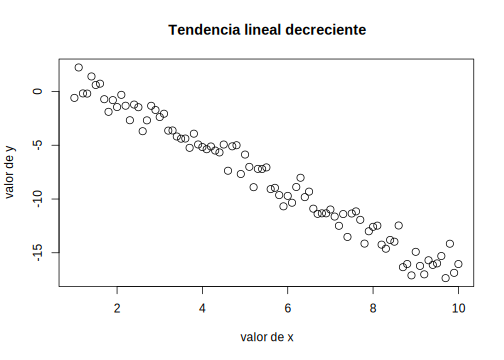
\includegraphics[keepaspectratio]{EstadisticaParaCienciasSocialesConR_files/figure-latex/unnamed-chunk-61-1.pdf}}

También se puede agregar una perturbación aleatoria, por ejemplo, valores aleatorios provenientes de una distribución normal con media uno y desviación estándar cero.

\begin{Shaded}
\begin{Highlighting}[]
\NormalTok{x }\OtherTok{\textless{}{-}} \FunctionTok{seq}\NormalTok{(}\DecValTok{1}\NormalTok{, }\DecValTok{10}\NormalTok{, .}\DecValTok{1}\NormalTok{)}
\NormalTok{y }\OtherTok{\textless{}{-}} \DecValTok{3} \SpecialCharTok{{-}} \DecValTok{2} \SpecialCharTok{*}\NormalTok{ x }\SpecialCharTok{+} \FunctionTok{rnorm}\NormalTok{(}\DecValTok{91}\NormalTok{)}
\FunctionTok{plot}\NormalTok{(x, y,}
  \AttributeTok{xlab =} \StringTok{"valor de x"}\NormalTok{, }\AttributeTok{ylab =} \StringTok{"valor de y"}\NormalTok{,}
  \AttributeTok{main =} \StringTok{"Tendencia lineal decreciente"}
\NormalTok{)}
\end{Highlighting}
\end{Shaded}

\pandocbounded{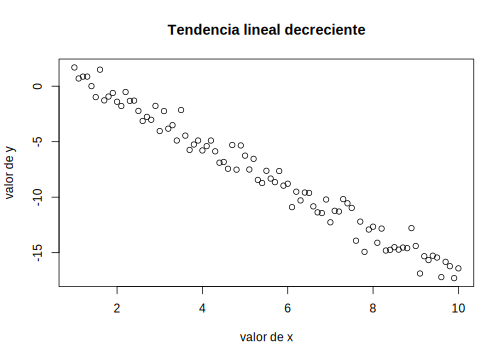
\includegraphics[keepaspectratio]{EstadisticaParaCienciasSocialesConR_files/figure-latex/unnamed-chunk-62-1.pdf}}

Cambie los coeficientes de la función lineal para probar los efectos en el gráfico.

\subsection*{Instalación de paquetes}\label{instalaciuxf3n-de-paquetes}
\addcontentsline{toc}{subsection}{Instalación de paquetes}

Cuando se descarga R y RStudio se cuenta con el sistema básico del lenguaje R. Las operaciones mencionadas en el apartado anterior y otras, están disponibles en esa base. Sin embargo, una gran cantidad de procedimientos están programados y ofrecidos como ``paquetes'', que sirven para tareas específicas. Su creación y desarrollo es parte de la potencialidad de R, porque son aportes de la comunidad que los diseña y los ofrece continuamente. En la actualidad hay más de 10000 paquetes en la CRAN (Comprehensive R Archive Network) aplicables a una gran diversidad de procedimientos.

La instalación de paquetes de R puede hacerse desde la línea de comando con la instrucción install.packages(``\,``) y el nombre del paquete entre comillas, también puede hacerse más directo, porque la IDE RStudio tiene, en el panel inferior derecho, una pestaña (la tercera) que dice \emph{packages} y en ella, una opción \emph{install} que abre una ventana para escribir (con autocompletado para los existentes) el nombre del paquete que se quiere instalar.\\
A lo largo del curso y en la medida que sea necesario, se cargarán paquetes específicos.

\part{Estadística Descriptiva}\label{part-estaduxedstica-descriptiva}

Debido a que la Estadística no trabaja con observaciones aisladas sino con conjuntos de ellas, siempre es necesario resumir la información, para presentarla de manera accesible a la lectura y para extraer significado.

Una gran tabla proveniente de registros hospitalarios que muestre las edades de madres primerizas no puede leerse de manera directa; es necesario buscar indicadores de síntesis, uno de ellos, muy difundido, es el promedio, un resumen de la información podría decir: ``En este hospital se atendieron durante el año 2024, 350 partos. Las madres tuvieron edades entre los 17 y los 45 años, con una edad promedio de 21''.

Sucede del mismo modo al observar los puntajes de una prueba de memoria aplicada a muchas personas o la distribución de votos luego de una elección. En esos casos podemos resumir esa información indicando el promedio (con las limitaciones que esta medida tiene). También es posible indicar cuántas personas tienen un valor menor a cierta cifra o mayor a otra: ¿cuántas de las madres primerizas son menores de 20 años?, ¿repiten de grado con igual frecuencia los varones que las mujeres? O bien expresar los valores a través de gráficos, que suelen aportar mucha información de manera abreviada (aunque también pueden ser engañosos).

Si de cada asistente a una escuela se conoce si repite el curso o no, la información agregada puede sintetizarse con la tasa de repitencia a nivel de la escuela, y expresar el resultado como: ``en esta escuela uno de cada quince estudiantes está repitiendo el curso''. Identificar un trending topic requiere observar una gran cantidad de tweets para detectar las repeticiones y las tendencias.

Entonces, la Estadística Descriptiva provee de una serie de procedimientos dirigidos a resumir, a sintetizar información, a volverla manejable para poder interpretarla y extraer conclusiones a partir del conjunto de datos que, de otra manera, serían ininteligibles.

\chapter{Los datos estadísticos}\label{los-datos-estaduxedsticos}

En este capítulo se desarrollan procedimientos para presentar la información de manera accesible para que pueda ser analizada y luego interpretada. Para poder extraer significado de los datos recogidos es necesario primero dedicar un esfuerzo a organizarlos, a presentarlos de manera comprensible, es una una operación previa a la aplicación de las técnicas de análisis que se verán más adelante.

La ciencia se interesa por la producción de conocimiento validado, uno de cuyos requisitos es que pueda ser comunicado de manera inequívoca, que se discutan las conclusiones a que llegan y los métodos que usan diferentes equipos de investigación, así como que los resultados que se publican puedan ser reproducidos por otros grupos de investigación. Esto implica la necesidad de usar un lenguaje que permita el intercambio al interior de las comunidades científicas y que dependa, en el menor grado posible, de las impresiones subjetivas o de las interpretaciones, o del modo en que cada integrante personalmente conciba los conceptos; en el intento de lograr un vocabulario tan unívoco como sea posible. Un modo de alcanzar esta comunicabilidad de las ideas, de los métodos y de los resultados, es definir, de la manera más precisa posible, los elementos acerca de los que se habla.\\
Alguna vez hemos dado con expresiones como ``esta persona es más inteligente que aquella''. ¿Qué se quiere decir exactamente con eso?, la afirmación podría provenir de algún evento en que se vio a esa persona actuando de manera que llamaríamos inteligente, aunque esto también puede confundirse con astucia: no es infrecuente usar el adjetivo inteligente para alguien a quien le resulta fácil engañar a otros y usar esos engaños para su beneficio; y, a la inversa, sería poco inteligente quien se deja engañar con facilidad. También suele decirse que alguien es inteligente porque obtiene buenos resultados en sus estudios. Esto es parte de la imprecisión en la definición de un concepto. Si se dispone de una definición de inteligencia, se puede saber cuándo aplicar esa idea a alguien, cuándo una conducta es inteligente, inclusive, cómo ayudar a desarrollar la inteligencia. Si se puede definir el concepto con el que se trabaja, se pueden indicar ciertas operaciones a realizar para evaluarlo y así conocer cuál es el nivel de inteligencia de una persona en particular.\\
Luego de definir el concepto con el que se trabaja, se requiere diseñar un instrumento que refleje esa definición y finalmente aplicar este instrumento a las personas que serán evaluadas. Al hacer esto último se obtiene un resultado que, si se expresa de manera cuantitativa, permite hacer comparaciones del aspecto que representa ese concepto, entre personas, entre grupos, etc.\\
¿Pueden compararse personas? La respuesta es no, porque cada persona tiene una infinidad de aspectos que la caracterizan y la hacen única. Por el contrario lo que sí pueden compararse son características claramente definidas de las personas. Del mismo modo no se pueden comparar escuelas, ni hogares, ni países si no se especifica en qué aspecto se realiza la comparación. O dicho de otro modo, cuál es la característica que se compara, y cómo se mide esa característica.\\
Podemos decir que una persona tiene más escolarización formal que otra, indicando con eso que ha aprobado más años de la escuela o de la universidad. Podemos decir que un hogar es diferente a otro si uno se compone de una pareja sola y el otro incluye una hija y dos hijos. Un país puede tener más habitantes, un régimen político diferente, o mayor libertad de expresión que otro. En todos los casos especificamos una característica (un rasgo o un estado), sobre la base del cual hacemos la comparación.

\section{La selección de la información pertinente}\label{la-selecciuxf3n-de-la-informaciuxf3n-pertinente}

Cuando se ha decidido quienes son los entes de la observación; es decir, una vez que se sabe a quiénes se observará, deben elegirse ciertas características que serán observadas\footnote{La palabra observar aquí se utiliza en un sentido general, puede tratarse de una observación directa como la que se realiza al mirar (o filmar) un comportamiento, o bien de la presentación de preguntas que alguien debe responder.}. Cada unidad que resulta de interés para la investigación tiene un conjunto muy grande de características observables y siempre se realiza una selección de esas características. Se trata de un recorte que permite comprender mejor ciertos aspectos, dejando de lado otros. La información que seleccionamos para observar se denomina pertinente para la investigación. Esta información puede provenir de diferentes fuentes, de manera general se distinguen dos tipos de fuentes: relevamientos y registros.\\
Los \textbf{relevamientos} pueden ser censos, encuestas u observaciones experimentales, y recogen información en un momento dado, en un corte transversal; una especie de foto que toma nota de un conjunto de características de las entidades, en el instante que se realiza: un día, una semana, el momento antes y después, etc. Por ejemplo, un censo se hace en uno o dos días, una vez cada diez años y, casa por casa, se recoge información sobre sexo, edad, estudios, lugar de necimiento, etc. de todas las personas que viven en cada hogar de todo el país. Una encuesta de opinión selecciona a algunos hogares y en ellos selecciona una persona en condiciones de votar, para preguntarle a quién piensa votar, qué opina da los diferentes partidos políticos, etc. La observación puede ser directa, como cuando se anota lo que se ve en un evento (una ceremonia por ejemplo) o un espacio (el patio de una escuela), pero a la que nos referimos aquí es la que está estructurada, aquella en la se explicita qué se observa. Esta etapa de la investigación, que es de producción de los datos, se llama ``trabajo de campo'', también puede ser telefónico o vía web, en todos los casos, dura un tiempo y se termina.\\
Los \textbf{registros} son continuos, lo que quiere decir que captan información a medida que esta se produce o bien a intervalos regulares. No empiezan y terminan, son estables, van captando los acontecimientos mientras suceden, o mejor dicho, mientras son informados. Ejemplos de estos registros son los registros civiles (de nacimientos, uniones, defunciones), de ingresos a hospitales, de inscripción a la universidad, de frontera, etc. En cualquier momento se pueden consultar y conocer lo que está registrado hasta ese momento, por ejemplo, cuántos nacimientos se asentaron en una ciudad en un año dado. O cuántos de esos nacimientos fueron de madre menor de 16 años.\\
- Relevamientos producen datos de stock (instantáneo).\\
- Registros producen datos flujo (continuo).

Cualquiera sea la fuente de los datos, una vez que se decide cuál es la información pertinente, se la recaba de varias de las entidades definidas y se cambia la óptica desde el caso particular a la regularidad colectiva. Es un cambio desde la observación del caso hacia la mirada puesta en el grupo. La siguiente es una lista que indica el área en que les gustaría trabajar cuando se reciban, a nueve estudiantes de primer año de Psicología:

\begin{longtable}[]{@{}lr@{}}
\caption{\label{tab:preferida}Área de trabajo preferida.}\tabularnewline
\toprule\noalign{}
Estudiante & Área \\
\midrule\noalign{}
\endfirsthead
\toprule\noalign{}
Estudiante & Área \\
\midrule\noalign{}
\endhead
\bottomrule\noalign{}
\endlastfoot
Susana & Clínica \\
Marcos & Laboral \\
Daniel & Clínica \\
Federico & Social \\
María & Clínica \\
Pedro & Educacional \\
Eugenia & Clínica \\
Mabel & Educacional \\
Francisco & Laboral \\
\end{longtable}

La lista reconoce a cada estudiante por su nombre, indica qué área le gustaría a cada cual y solo indica eso, no se sabe su edad, ni cuáles son sus intereses políticos ni el deporte favorito, solo se seleccionó como pertinente para este ejemplo, el área en que le gustaría trabajar. Si ahora se transforma esa lista en una tabla:

\begin{longtable}[]{@{}lr@{}}
\caption{\label{tab:unnamed-chunk-66}Área de trabajo preferida.}\tabularnewline
\toprule\noalign{}
Área & Casos \\
\midrule\noalign{}
\endfirsthead
\toprule\noalign{}
Área & Casos \\
\midrule\noalign{}
\endhead
\bottomrule\noalign{}
\endlastfoot
Clínica & 4 \\
Educacional & 2 \\
Laboral & 2 \\
Social & 1 \\
\end{longtable}

Se lee que Clínica es un área preferida por cuatro estudiantes, Laboral y Educacional atrae a dos y a Social solo tiene una mención. Las personas desaparecieron, ya no hay nombres, hemos abstraído para referirnos al área preferida, no a las personas que las prefieren. En la tabla se ve que lo más frecuente es que se prefiera Clínica, y que Social es poco frecuente. Se pasó de la lista de personas reconocibles a la tabla de valores. Nos despegamos de los casos a fin de buscar la regularidad en el conjunto. Más adelante diremos que se ha pasado de la matriz de datos a la distribución de frecuencias, que constituye una reducción o un primer resumen de la información disponible. Esta operación es menos obvia de lo que puede parecer y es tardía en la historia de las ideas, tiene origen en la publicación, de \citet{gaunt1662} ``Observaciones naturales y políticas hechas sobre los boletines de mortalidad'', quien tomó las listas de defunciones sucedidas en Londres durante veinte años en tiempos de la peste y las resumió en orden cronológico. Su operación fue la de cambiar la lista por la tabla, para observar al proceso (la mortalidad a lo largo del tiempo), en lugar de las muertes registradas individualmente.

Consideremos el siguiente cuestionario, que se aplicó en 2019 a personas con edades 18 y 35 años.

\begin{figure}[H]

{\centering 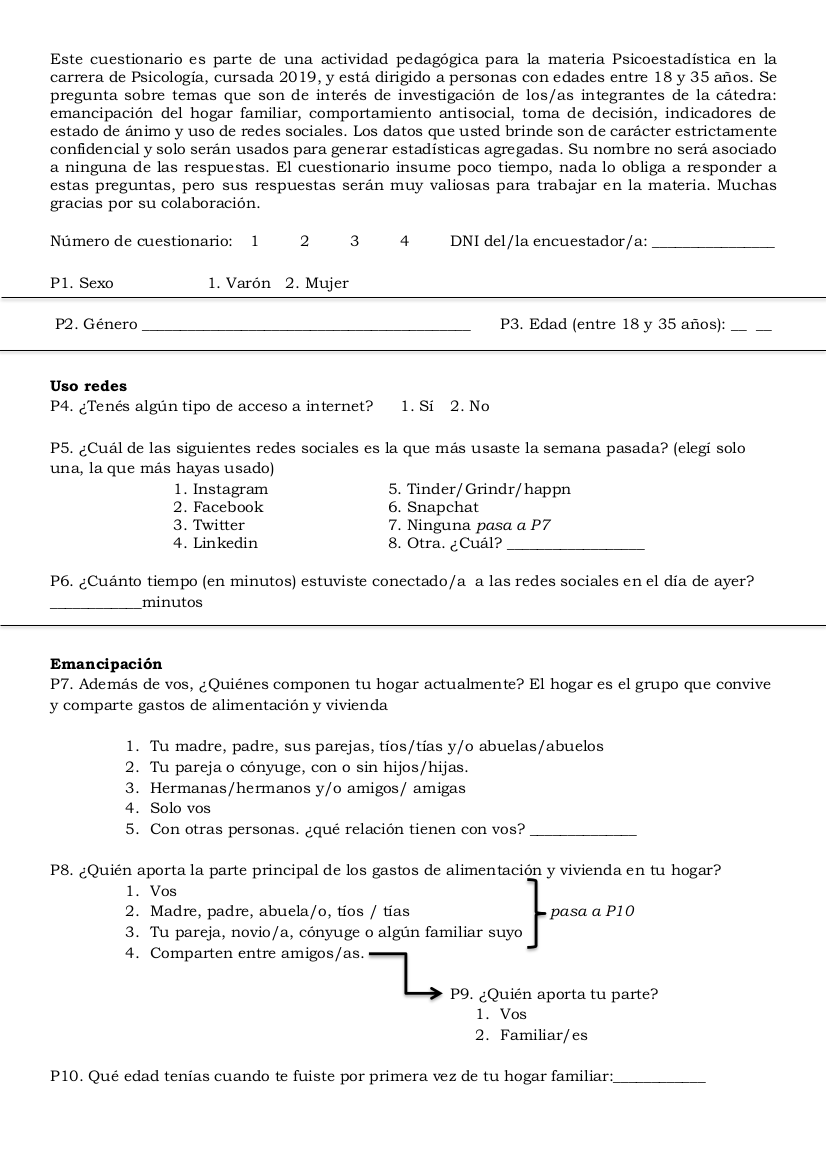
\includegraphics[width=0.8\linewidth]{imagenes/cuestionario2019_01} 

}

\caption{Cuestionario 2019}\label{fig:cuestionario-1}
\end{figure}
\begin{figure}[H]

{\centering 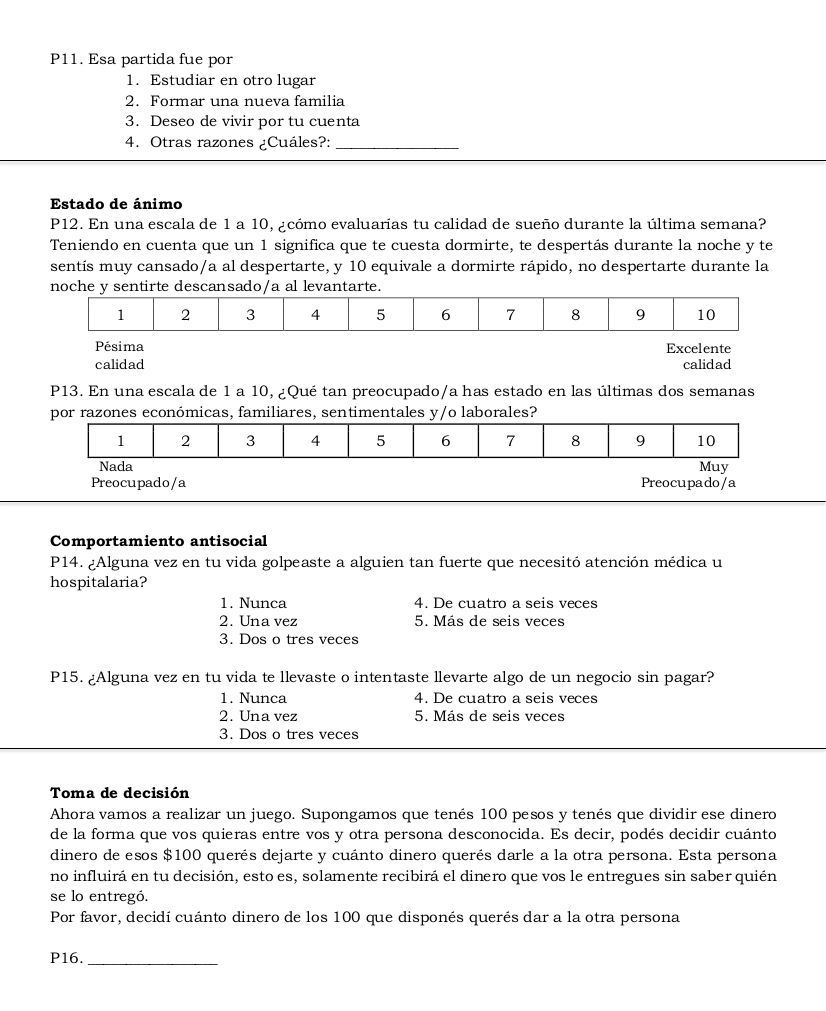
\includegraphics[width=0.8\linewidth]{imagenes/cuestionario2019_02} 

}

\caption{Cuestionario 2019}\label{fig:cuestionario-2}
\end{figure}

Este instrumento de producción de datos, se dirigió a una población definida: personas entre 18 y 35 años. En él se solicitó información sobre un conjunto seleccionado de características; los ítems numerados desde P1 hasta P16. Se trata de unos pocos aspectos de cada persona los que interesan para esta investigación; no se tiene en cuenta, por ejemplo la opinión política de quienes responden, ni su estatura o la región en que viven. Estas últimas y muchas más son características de estas personas, pero están fuera del alcance de la investigación. Esto muestra a qué nos referimos con que la información seleccionada constituye un recorte, es una parcialización de las entidades (no siempre son personas) que responden, en la que se eligen solo los aspectos que son de interés para una investigación particular.\\
El cuestionario tiene 16 ítems, cada persona que lo responde marca una sola de las opciones indicadas en cada ítem. Una vez completados los cuestionarios, la información está ``en bruto'' y es necesario ordenarla para poder tener una visión de conjunto. Eso se logra organizando los datos recogidos en la \emph{matriz de datos} que es equivalente a la lista de la tabla \ref{tab:preferida}, pero con más aspectos relevados que solo el área preferida. Para el cuestionario mostrado, el siguiente es un fragmento de esa lista:

\begin{verbatim}
##    sexo edad acceso.redes red.usada red.otra tiempo.red
## 1 mujer   19           si Instagram     <NA>        120
## 2 varón   29           si  Facebook     <NA>         90
## 3 mujer   31           si  Facebook     <NA>         30
## 4 mujer   28           si      Otra    gmail         30
## 5 mujer   22           si Instagram     <NA>        120
## 6 varón   22           si  Facebook     <NA>        240
\end{verbatim}

Este ordenamiento rectangular de la información tiene filas (horizontales) y columnas (verticales), en esta imagen solo se ven las primeras seis filas y seis columnas de la matriz. Cada fila es una persona que respondió y cada columna es un ítem. La primera fila es el encabezado, y muestra los nombres de los ítems del cuestionario (en este ejemplo solo los seis primeros) y las seis filas mostradas, indican las respuestas dadas por los encuestados. Así, la persona que respondió al primer cuestionario es una mujer, que tiene 19 años, tiene acceso a redes sociales y la que más usa es Instagram, como no respondió ``otra'', en la columna siguiente tiene , que indica que no hay dato allí (Not Available), dedica en promedio 120 minutos diarios a las redes y así sigue toda la fila correspondiente a esa persona, que no está mostrada aquí por razones de espacio.

La matriz de datos contiene toda la información que será insumo de los análisis posteriores, luego será necesario definir qué es cada elemento que la constituye.

\begin{longtable}[]{@{}
  >{\centering\arraybackslash}p{(\linewidth - 0\tabcolsep) * \real{1.0000}}@{}}
\toprule\noalign{}
\endhead
\bottomrule\noalign{}
\endlastfoot
La matriz de datos es un arreglo en el que cada fila (horizontal) representa una de las entidades de la cual proviene la información, cada columna (vertical) es un aspecto de esas entidades, que se ha seleccionado para observar, y cada celda es el valor que tiene la entidad de la fila en el aspecto de la columna correspondiente. \\
\end{longtable}

\section{Las entidades}\label{las-entidades}

Hemos dicho que cada fila representa un caso, una entidad a la que se observa. Puede ser una persona como en este ejemplo, pero también una entidad colectiva: un hogar, una empresa, una escuela, un animal de laboratorio, un país. Cada una de ellas se denomina \textbf{unidad de análisis}.

Es importante que las unidades de análisis estén claras para la interpretación de los resultados. Por ejemplo, si se afirma que ``las personas de menores recursos acceden menos frecuentemente a la educación superior'', hablamos de personas, y éstas son las unidades de análisis. Y es muy diferente a decir que ``en los países más pobres, es menor la proporción de personas que acceden a la educación superior'', porque aquí las unidades de análisis son los países.

\begin{longtable}[]{@{}
  >{\centering\arraybackslash}p{(\linewidth - 0\tabcolsep) * \real{1.0000}}@{}}
\toprule\noalign{}
\endhead
\bottomrule\noalign{}
\endlastfoot
Las \textbf{unidades de análisis} son los entes individuales acerca de los que se analizan sus cualidades. \\
\end{longtable}

Si las unidades de análisis fuesen escuelas, sus características, dependiendo de la investigación de que se trate, podrían ser: sector de gestión (estatal o privada), nivel (primaria, secundaria, ambas), cantidad de bancos por aula (\#), turnos (mañana, tarde, ambos), etc. Si se tratara de hogares, puede observarse: cantidad de miembros, composición, actividad económica, etc. Si se observan países, sus características de interés pueden ser: su régimen político, cantidad de habitantes, distribución de la riqueza, etc.

\section{Las variables}\label{las-variables}

Cada columna de la matriz de datos es un ítem del cuestionario, es decir un aspecto seleccionado de las unidades de análisis hacia el cual se dirige la atención, que se consideró necesario para la investigación. Esos aspectos se denominan \textbf{variables}. Así, el \emph{sexo} es una variable, como lo es \emph{con quién vive}, \emph{cuánto daría en el experimento}, etc. Cada ítem del cuestionario se constituye en una variable, a veces su expresión interrogativa en el cuestionario se transforma en algo más abreviado, como la pregunta: ``¿Cuánto tiempo (en minutos) estuviste conectado/a a las redes sociales en el día de ayer?'' se trata como la variable \emph{tiempo.red}. Las variables son los aspectos de las entidades que se someterán al análisis, aquellos aspectos que se han seleccionado como información pertinente para un estudio en particular. Su cualidad central es la que le da nombre: la de variar.

\begin{longtable}[]{@{}
  >{\centering\arraybackslash}p{(\linewidth - 0\tabcolsep) * \real{1.0000}}@{}}
\toprule\noalign{}
\endhead
\bottomrule\noalign{}
\endlastfoot
Una \textbf{variable} es una característica de las unidades de análisis que puede asumir diferentes valores en cada una de ellas. \\
\end{longtable}

Cada vez que se haga referencia a una variable, debe conocerse cuál es la unidad de análisis a la que se refiere, si no resulta claro, se debe indicar. Es diferente afirmar que un país es rico que decir que sus habitantes lo son.

\section{Las categorías}\label{las-categoruxedas}

El cuerpo de la matriz de datos tiene números que corresponden a las respuestas que cada respondente dio a cada ítem. En la primera fila, primera columna dice ``mujer'' esa es la respuesta que dio esa persona. En esta pregunta, se podía elegir entre dos respuestas diferentes (varón, mujer), en el lenguaje que estamos introduciendo, diremos que esta variable (\emph{sexo}) puede asumir dos \textbf{categorías} diferentes. Para el primer caso, la variable \emph{sexo} asume la categoría ``mujer''. Las categorías son las posibilidades que tiene una variable, son sus alternativas, dentro de las cuales a todas las unidades de análisis les corresponde una y solo una.

\begin{longtable}[]{@{}
  >{\centering\arraybackslash}p{(\linewidth - 0\tabcolsep) * \real{1.0000}}@{}}
\toprule\noalign{}
\endhead
\bottomrule\noalign{}
\endlastfoot
Las \textbf{categorías} de una variable son los valores que ésta puede asumir. \\
\end{longtable}

Cada vez que se define una variable ─es decir cada vez que se selecciona un aspecto de las unidades de análisis para observar─, debe indicarse también el conjunto de categorías que le corresponden, aunque a veces esto está implícito. Si la variable es \emph{nivel de escolaridad alcanzado}, pueden considerarse las siguientes categorías: ``ninguno'', ``primario incompleto'', ``primario completo'', ``secundario incompleto'', ``secundario completo'', ``terciario o universitario incompleto'', ``terciario o universitario completo'' y ``postgrado''. Si tratamos con la variable \emph{edad}, sus categorías son valores numéricos, entre cero y un máximo de años que se fija según el caso.

\subsection{Requisitos de las categorías}\label{requisitos-de-las-categoruxedas}

Hay dos propiedades que debemos asegurar que cumplan las categorías que construyamos. La primera se llama \textbf{exclusión mutua}, es decir que cada categoría excluya a todas las demás. Dicho de otra manera, si a una unidad de análisis le corresponde una categoría, entonces sabemos que no le corresponde ninguna otra. Si analizamos hogares y a cada persona le preguntamos por su parentesco, sin indicar con quién, tendremos una categorización defectuosa, porque una persona del hogar puede al mismo tiempo ser hijo y hermano, o hija y madre, si conviven tres generaciones. En cualquiera de los dos casos, a una misma persona le corresponderían dos categorías y se viola el requisito de exclusión mutua. Esto se resuelve estableciendo respecto de quién se declara el parentesco, y cada integrante del hogar lo refiere a la misma persona\footnote{A quien se llama ``Jefe o jefa de Hogar''.}.

Al analizar los tipos de lectura preferida, nos equivocaríamos si los categorizáramos como de ficción, de misterio, policiales, románticas, biográficas, de aventuras; ya que la categoría ficción puede incluir misterio, policiales, novelas románticas o de aventuras.

También se comete ese error si se clasifica a las escuelas como céntricas, parroquiales, urbanas y rurales. Dado que una escuela puede ser al mismo tiempo parroquial y urbana. Es necesario separar, para que quede claro, lo que interesa en el análisis: si lo que queremos distinguir son escuelas céntricas de barriales, entonces la variable será la ubicación geográfica y no importa si la escuela depende de una iglesia o del estado; es decir, primero identificar la variable (que aspecto se quiere observar) y luego sus categorías (cuáles son las posibilidades de ese aspecto).

\begin{longtable}[]{@{}
  >{\centering\arraybackslash}p{(\linewidth - 0\tabcolsep) * \real{1.0000}}@{}}
\toprule\noalign{}
\endhead
\bottomrule\noalign{}
\endlastfoot
Las categorías de una variable son \textbf{mutuamente excluyentes} si a cada individuo le corresponde no más de una categoría. \\
\end{longtable}

El segundo requisito que solicitaremos a las categorías de una variable es que agoten todas las posibilidades de variación, es decir, que todos los valores posibles estén contemplados. Esta cualidad se llama \textbf{exhaustividad}.

Veamos qué sucede si no respetamos este requisito. Si evaluamos la variable situación conyugal y ofrecemos como categorías: ``casada/casado'', ``soltera/soltero'', ``divorciada/divorciado'', ``viuda/viudo''; las personas que estén viviendo juntas sin estar casadas no encuentran un lugar donde ubicarse, como tampoco lo encuentran quienes están separados sin haberse divorciado. Para resolver esto es necesario, o bien incluir estas categorías explícitamente, agregando ``unida/unido'', ``separada/separado''; con lo que se amplía el número de categorías, o bien fusionarlas con las existentes: ``casada/casado o unida/unido'', ``soltera/soltero'', ``separada/separado o divorciada/divorciado'', ``viuda/viudo''.\\
Con la edad, las categorías son valores numéricos que pueden ir del cero hasta el un máximo, pero ¿dónde fijarlo? Si se eligiera un límite como 100 años, algunas personas quedarían fuera, quizás sean pocas, pero no pueden quedar sin categoría donde incluirse. Por lo demás, puede haber solo una persona de 103 años, otra de 105, por lo que no se justifica seguir extendiendo categorías. Una solución frecuente es la de tomar una categoría abierta final, fijando como última categoría ``100 y más'', e incluir allí a todas las personas que declaren una edad de 100 años o superior. Puede verse que esta opción conlleva una pérdida de información, ya que no sabemos la edad exacta de quienes se ubican en esa categoría. Aceptamos esa pérdida a cambio de reducir el número de categorías de la variable, luego volveremos sobre eso.\\
Algunas preguntas de cuestionarios, luego de un conjunto de opciones para responder, incluyen una categoría que dice ``Otro\(\ldots\) especificar''. Se trata de casos de categorizaciones en las que no se sabe de antemano cuáles son todas las respuestas posibles; son frecuentes en las encuestas de opinión. Por ejemplo, si alguien declara que en las próximas elecciones va a votar en blanco y preguntamos por qué, podemos conocer de antemano algunas de las respuestas posibles, pero debemos dejar espacio para que se expresen razones que no habíamos previsto. De este modo aseguramos la exhaustividad de las categorías. En el cuestionario del ejemplo, la P7 tiene, en la opción 5, la posibilidad de otras alternativas de convivencia, aparte de las ofrecidas.

\begin{longtable}[]{@{}
  >{\centering\arraybackslash}p{(\linewidth - 0\tabcolsep) * \real{1.0000}}@{}}
\toprule\noalign{}
\endhead
\bottomrule\noalign{}
\endlastfoot
Las categorías de una variable son \textbf{exhaustivas} si todo individuo tiene alguna categoría que le corresponda. \\
\end{longtable}

En algunas situaciones, el número de categorías de una variable es parte de las decisiones de la investigación. Hay casos en que las categorías están establecidas de antemano: por ejemplo, en la variable sexo se tiende a usar como categorías las de varón y mujer; sin embargo, si estamos frente a un estudio que trate precisamente sobre identidad de género, deberá considerarse un espectro más amplio de categorías, o bien ofrecer preguntas abiertas, sin establecer categorías de antemano. Como ha sido el caso de P2 en el cuestionario, que no ha sido cargada en la matriz de datos, porque requiere una codificación posterior.\\
Como se señaló, en la edad de las personas suele elegirse terminar las categorías con ``100 y más''. De hecho, también se podrían mantener las edades exactas hasta 109 años y cerrar con 110 y más. Qué se elija depende de cuánta información y cuánta claridad se decida que tenga la clasificación; lamentablemente, no es posible lograr al mismo tiempo el máximo de información y de claridad en la presentación\footnote{A menudo que, en Estadística, es necesario llegar a puntos de equilibrio entre el grado de detalle de la información que se ofrece y la claridad con que esa información puede presentarse.}.

\section{Los símbolos numéricos}\label{los-suxedmbolos-numuxe9ricos}

Las categorías pueden tener diferente naturaleza: algunas se expresan con números (como la edad) y otras con palabras (como la carrera que cursa), otras en graduaciones (como el grado de acuerdo); sin embargo es muy común representar con números a las categorías, aun cuando lo que se observe no sea numérico. Así, en la variable nivel de educación, pueden codificarse las categorías de la siguiente manera:

\begin{longtable}[]{@{}cl@{}}
\caption{\label{tab:unnamed-chunk-68}Nivel de educación alcanzado.}\tabularnewline
\toprule\noalign{}
Código & Máximo nivel de educación formal alcanzado \\
\midrule\noalign{}
\endfirsthead
\toprule\noalign{}
Código & Máximo nivel de educación formal alcanzado \\
\midrule\noalign{}
\endhead
\bottomrule\noalign{}
\endlastfoot
1 & ninguno \\
2 & primario incompleto \\
3 & primario completo \\
4 & secundario incompleto \\
5 & secundario completo \\
6 & terciario o universitario incompleto \\
7 & terciario o universitario completo \\
8 & postgrado \\
\end{longtable}

Hemos usado números para referirnos a las categorías a fin de simplificar la notación.\\
De manera equivalente podemos codificar las categorías de otras variables:

\begin{longtable}[]{@{}cc@{}}
\caption{\label{tab:unnamed-chunk-69}Distribución por sexos.}\tabularnewline
\toprule\noalign{}
Código & Sexo \\
\midrule\noalign{}
\endfirsthead
\toprule\noalign{}
Código & Sexo \\
\midrule\noalign{}
\endhead
\bottomrule\noalign{}
\endlastfoot
1 & Varón \\
2 & Mujer \\
\end{longtable}

\begin{longtable}[]{@{}cl@{}}
\caption{\label{tab:unnamed-chunk-70}Satisfacción con el progreso en la carrera.}\tabularnewline
\toprule\noalign{}
Código & Estoy muy satisfecho con el modo en que he progresado en mi carrera \\
\midrule\noalign{}
\endfirsthead
\toprule\noalign{}
Código & Estoy muy satisfecho con el modo en que he progresado en mi carrera \\
\midrule\noalign{}
\endhead
\bottomrule\noalign{}
\endlastfoot
1 & Completamente en desacuerdo \\
2 & En desacuerdo \\
3 & Indiferente \\
4 & De acuerdo \\
5 & Completamente de acuerdo \\
\end{longtable}

En las variables cuyas categorías son numéricas, no es necesario hacer ninguna codificación. Así, la edad quedará expresada de manera numérica directamente por la cantidad de años, como sucede con la cantidad de materias aprobadas, el número de hijos e hijas o la cantidad de habitantes de un país. En estos casos, la exclusión mutua y la exhaustividad se cumplen sin más.

\section{La medición}\label{la-mediciuxf3n}

En Ciencias Sociales tiene plena vigencia el debate acerca de las posibilidades de medición de los fenómenos que se estudian. Buena parte de la discusión gira en torno a una definición de medición, ya que según qué sea lo que se considere como tal, se tratará de una medición o no. La posición más tradicional corresponde a lo que el sentido común trata como medición: la estatura, las distancias, el peso, etc. Esta definición demanda que los números que codifican a las categorías tengan algunas propiedades para considerarlos como mediciones. Se conoce como teoría clásica de la medición, y desde ese punto de vista sería muy difícil realizar mediciones sobre las variables que manejamos en Ciencias Sociales. Una definición menos restrictiva es la que propuso \citet{Stevens1946}, según la cual:

\begin{longtable}[]{@{}
  >{\centering\arraybackslash}p{(\linewidth - 0\tabcolsep) * \real{1.0000}}@{}}
\toprule\noalign{}
\endhead
\bottomrule\noalign{}
\endlastfoot
``medir es asignar números a los objetos según cierta regla, de manera que los números asignados en la medición, no representan propiamente cantidades, sino relaciones''. \\
\end{longtable}

Esta última definición, basada en la teoría representacional de la medición, es la que adoptaremos en este curso aunque la discusión sigue vigente. Desde esta definición, evaluar una variable para una unidad de análisis dada, equivale a medir esa unidad de análisis en el aspecto que la variable expresa.

Aun cuando se adopte una definición amplia de lo que es medir, podemos intuir que no se mide una opinión del mismo modo que se mide el salario o la estatura. Además, hay ocasiones en que la palabra \emph{medición} parece forzada. Si se asigna el número 1 a los varones y 2 a las mujeres, decir que con estos números se \emph{mide el sexo} es extraño. Por el contrario, resulta familiar \emph{medir la estatura} asignando a cada persona el número de centímetros que indica una cinta métrica. Sin embargo, desde la teoría representacional, ambas son mediciones. Esto sugiere que, dentro de las variables de las que hemos hablado hasta aquí habrá que reconocer diferencias, y estas diferencias vendrán dadas por el significado que tengan los números que asignamos a las categorías, es decir, por las reglas que ligan los números con lo que se observa.

\begin{longtable}[]{@{}
  >{\centering\arraybackslash}p{(\linewidth - 0\tabcolsep) * \real{1.0000}}@{}}
\toprule\noalign{}
\endhead
\bottomrule\noalign{}
\endlastfoot
El \textbf{nivel de medición} de una variable está determinado por el significado que tengan los símbolos numéricos que se asignan a las categorías. \\
\end{longtable}

Existe una graduación en el significado que tienen los números, y por eso se habla de niveles, que pueden ser más altos o más bajos. En la variable \emph{sexo}, haber elegido ``1'' para varones y ``2'' para mujeres es de una arbitrariedad total (de la que alguien podría quejarse). Si la codificación hubiese sido al revés, habría estado igual de bien, y también habría estado bien usar el número ``75'' para representar a los varones y el ``38'' para las mujeres, aunque esto resulta un poco incómodo. Por el contrario, en la variable \emph{edad}, asignar el número ``20'' a quien tiene 20 años, parece totalmente ``natural'' ¿qué otro número podríamos haber asignado? ¿Qué sucede con el \emph{nivel de educación}? En el ejemplo elegimos numerar las categorías del 1 al 8; habría habido otras opciones, por ejemplo usar solo números pares o números impares u otra secuencia arbitraria, pero algo importante es que cualquier secuencia que se elija debe respetar el orden de las categorías de la variable, por lo que los números deben reflejarlo; no habría sido correcto usar números que no vayan aumentando, como lo hacen los niveles de educación.

Así entonces, hay grados diferentes en la libertad que existe para asignar los números a las categorías. Esas diferencias distinguen los niveles de medición de las variables.

\subsection{Niveles de medición}\label{niveles-de-mediciuxf3n}

Según la mayor o menor arbitrariedad que exista en la relación que liga los números a las categorías, hablaremos de diferentes niveles de medición: cuánta más restricción haya en la asignación de los números a las categorías, más alto será el nivel de medición de las variables. Cuanto más alto sea el nivel de medición, mayores son las propiedades que tienen los números, es decir son más amplias las operaciones que puede hacerse son ellos. Si los números se asignan de manera totalmente arbitraria, el nivel de medición es el más bajo de todos y se llama \textbf{nivel nominal} (como en la variable \emph{sexo}); si los números deben respetar el orden de las categorías (como en la \emph{educación}), la variable se llama de \textbf{nivel ordinal}. Por ahora, nos detenemos en estos dos niveles.

\subsubsection{El nivel nominal}\label{el-nivel-nominal}

Es el nivel más elemental de medición: las variables de este nivel tienen categorías que son solo nombres (de allí que se llamen nominales). La asignación de códigos numéricos cumple la función de designar las categorías, es decir, de distinguirlas unas de otras. Por ejemplo, \emph{área de especialización preferida} (UA = estudiantes de Psicología) y \emph{carrera que cursa} (UA = estudiantes de nivel universitario), podrían tener las siguientes codificaciones:

\begin{longtable}[]{@{}clcl@{}}
\caption{\label{tab:nivelNomCod}Ejemplos de codificación de variables nominales.}\tabularnewline
\toprule\noalign{}
Código & Carrera & Código & Área \\
\midrule\noalign{}
\endfirsthead
\toprule\noalign{}
Código & Carrera & Código & Área \\
\midrule\noalign{}
\endhead
\bottomrule\noalign{}
\endlastfoot
1 & Psicología & 1 & Clínica \\
2 & Filosofía & 2 & Educacional \\
3 & Medicina & 3 & Jurídica \\
4 & Otras & 4 & Laboral \\
& & 5 & Sanitaria \\
& & 6 & Social \\
& & 7 & Experimental \\
& & 8 & Otra \\
\end{longtable}

Por comodidad, se empieza en el ``1'' y desde allí correlativamente, pero no hay ninguna prohibición para codificar con cualquier conjunto de números. Aun con esta amplia libertad para elegir los códigos numéricos, hay algo que no se puede hacer: no es válido usar el mismo número más de una vez. Si hiciéramos esto, confundiríamos las categorías que corresponden a cada individuo. Así, a un estudiante de Psicología, le asignamos el valor ``1'' en la variable \emph{carrera}, ya no podría usarse ese mismo número en la misma variable también para alguien que estudia Medicina. Diremos que la condición que deben cumplir los números en este nivel de medición es que: a categorías diferentes correspondan números distintos.\\
Entonces, en este nivel de medición a cada categoría puede asignarse, de manera arbitraria, uno y solo un número. Esta forma de asignar los valores numéricos solo implica que éstos designan las categorías (que las distinguen a una de otra), por eso, no es posible tratarlos como números en cuanto a sus propiedades aritméticas. En particular no puede sumárselos: nada puede significar que se sumen los números ``1'' y ``2'' que codifican a las carreras de Psicología y Filosofía.

\begin{longtable}[]{@{}
  >{\centering\arraybackslash}p{(\linewidth - 0\tabcolsep) * \real{1.0000}}@{}}
\toprule\noalign{}
\endhead
\bottomrule\noalign{}
\endlastfoot
Una variable está medida a nivel \textbf{nominal} si los números que representan cada categoría son asignados de manera arbitraria y solo cumplen con la función de designar y distinguir categorías diferentes. \\
\end{longtable}

Para unidades de análisis medidas a través de una variable de nivel nominal, es posible saber si corresponden a la misma categoría o a una diferente, es decir si tienen la misma cualidad (o atributo) o una diferente.

En la tabla \ref{tab:nivelNomCod} si a una persona le corresponde el número ``1'' y a otra también, podemos decir que coinciden en esta variable, ambas estudian la misma carrera (Psicología), y si a una le corresponde el ``1'' y a otra el ``3'', sabremos que la primera estudia Psicología y la otra Medicina. El hecho que el número ``3'' sea más grande que el ``1'', no tiene ninguna interpretación en este nivel de medición, no puede decirse que Psicología sea menos que Medicina. Como tampoco vale que ``3'' sea el triple de ``1''.

Si ``1'' y ``2'' son dos categorías de una variable medida a nivel nominal, el único tipo de relación que puede establecerse entre ellas es \[1\neq2\]
Es decir que 1 es diferente de 2.

La regla de transformación de una escala nominal en otra es que cualquier número puede cambiarse por cualquiera a condición de no repetir ninguno. La escala nominal ``1'', ``2'', ``3'', ``4'' puede cambiarse por la ``5'', ``8'', ``4'', ``2''. Aunque no es obligatorio, en la práctica, lo más frecuente es usar los primeros números naturales para codificar las categorías.

\subsubsection{El nivel ordinal}\label{el-nivel-ordinal}

Aquí subimos un nivel, ya que a los números que solo tienen la propiedad de designar en las variables nominales, se agrega otra: la de reflejar el orden que existe entre las categorías.
Simplemente ahora se trata de variables cuyas categorías indican alguna cualidad de las unidades de análisis que crece en una dirección. Eso equivale a decir que se pueden hacer entre ellas, juicios de orden, tales como una categoría es mayor que otra, una categoría es menor que otra. El \emph{grado de escolarización} cumple con ese requisito: efectivamente, el ``primario incompleto'' es un nivel de estudios superior a ``ninguno'', pero inferior a ``primario completo''.
Los valores numéricos que representan las categorías rescatan ahora una propiedad adicional: el orden. Además de poder distinguir si dos sujetos tienen la misma característica analizada o una distinta, como en el nivel nominal, ahora también podemos saber si un individuo tiene esa característica en mayor o menor grado. Así como ``ninguno'' es menor que ``primario incompleto'', los números correspondientes cumplen con que ``1'' es menor que ``2'' y resulta más sencillo escribirlo como \[1 < 2\].

\begin{longtable}[]{@{}
  >{\centering\arraybackslash}p{(\linewidth - 0\tabcolsep) * \real{1.0000}}@{}}
\toprule\noalign{}
\endhead
\bottomrule\noalign{}
\endlastfoot
Una variable está medida a nivel \textbf{ordinal} si los números que representan cada categoría son asignados de manera que respeten el orden según aumenta o disminuye la característica que la variable mide. \\
\end{longtable}

Estos números designan las categorías y son expresión de la jerarquía que hay entre ellas. Otro ejemplos de variable medida a nivel ordinal y su correspondiente codificación numérica es la pregunta ¿Alguna vez en tu vida golpeaste a alguien tan fuerte que necesitó atención médica u hospitalaria? (P14) del cuestionario, que fue codificada de manera creciente con la intensidad:

\begin{longtable}[]{@{}cl@{}}
\caption{\label{tab:unnamed-chunk-72}Ejemplo de codificación de una variable ordinal.}\tabularnewline
\toprule\noalign{}
Código & P14 \\
\midrule\noalign{}
\endfirsthead
\toprule\noalign{}
Código & P14 \\
\midrule\noalign{}
\endhead
\bottomrule\noalign{}
\endlastfoot
1. & Nunca \\
2. & Una vez \\
3. & Dos o tres veces \\
4. & De cuatro a seis veces \\
5. & Más de seis veces \\
\end{longtable}

De aquí en adelante ya no usaremos una columna especial de la tabla para indicar el código, simplemente lo señalamos junto al nombre de la categoría, encabezado con el nombre abreviado de la variable:

\begin{longtable}[]{@{}l@{}}
\caption{\label{tab:unnamed-chunk-73}Ejemplo de una variable ordinal codificada.}\tabularnewline
\toprule\noalign{}
Golpeó \\
\midrule\noalign{}
\endfirsthead
\toprule\noalign{}
Golpeó \\
\midrule\noalign{}
\endhead
\bottomrule\noalign{}
\endlastfoot
1. Nunca \\
2. Una vez \\
3. Dos o tres veces \\
4. De cuatro a seis veces \\
5. Más de seis veces \\
\end{longtable}

Acerca del significado de los valores numéricos en las variables de nivel ordinal, si bien hemos agregado el orden, aun no es posible hacer operaciones con ellos. Es decir, no es posible sumar dos valores y que la suma tenga algún significado. Por ejemplo, en la última variable, no es cierto que \(3 = 2+1\), porque no es cierto que ``dos o tres veces'' sea lo mismo que ``nunca'' más ``una vez''. Tampoco es válido restarlos, veamos que la diferencia entre 1 y 2 es 1 y la diferencia entre 4 y 5 también es 1, pero eso no tiene un correlato entre las categorías: no es cierto que haya la misma distancia entre ``nunca'' y ``una vez'' que entre ``de cuatro a seis'' y ``más de seis'', simplemente porque no tenemos definida la idea de \emph{distancia} para esta variable.\\
Si ``1'' y ``2'' son dos categorías de una variable medida a nivel ordinal, se pueden establecer las relaciones: \[1 \neq 2\] y \[1<2\] Es decir que, uno es diferente que dos y que uno es menor que dos. A la relación de distinción que existe entre categorías de la escala nominal se agrega la relación de orden.

La regla de transformación de una escala ordinal en otra consiste en cambiar los números por cualquiera, a condición que no se repita ninguno (como en la nominal) y además, que sigan el mismo orden. La escala ordinal ``1'', ``2'', ``3'', ``4'' puede cambiarse por la ``5'', ``8'', ``15'', ``23''. Nuevamente, esto es poco común y suelen usarse números correlativos.

Los dos niveles (o escalas) de medición siguientes se llaman intervalares y proporcionales y usan las codificaciones numéricas con un significado un poco diferente al visto hasta aquí. La principal diferencia es que el grado de arbitrariedad para asignar los números se reduce sustancialmente. En primer lugar, las escalas intervalares conservan las distancias entre los valores. En las variables medidas a nivel proporcional, además de conservarse la distancia, se verifica la proporcionalidad de los valores: es decir que, recién en estas escalas, cuatro será el doble de dos.

\subsubsection{El nivel intervalar}\label{el-nivel-intervalar}

Veamos un ejemplo antes de definir este nivel. Cuando decimos que estamos en el año 2020, hacemos implícitamente una afirmación que supone una medición del tiempo transcurrido desde un determinado evento, cuya elección no es única. En cierto modo decimos ``han transcurrido 2020 años desde el momento que se acordó usar como inicio de este calendario''. En culturas no cristianas, el origen en la medición de los tiempos puede ubicarse en otro momento y, en consecuencia, el año actual es otro. En el calendario judío, por ejemplo, el presente es el año 5780. Hay entonces libertad para decidir la ubicación del punto desde donde empezar a contar los años. Lo que podría llamarse el ``año cero'', no es necesariamente el mismo. Sin embargo, el tiempo transcurrido entre la Toma de la Bastilla en París y la Toma del Palacio de Invierno en Petrogrado es de 128 años, que es el período entre 1789 y 1917 en el calendario gregoriano y entre 5549 y 5677 según el calendario judío. Es decir que la transformación que lleva los años de un calendario al otro, conserva las distancias. Independientemente de la escala con que hayamos medido el año, la diferencia entre dos años, se mantiene constante. Eso sucede porque las dos escalas (en este ejemplo, la medición del tiempo según las tradiciones cristiana y judía) se distinguen solo en la elección del origen (la posición del cero) pero no en la definición de lo que es un año. Para ambas escalas un año corresponde a una vuelta de la tierra al sol, por lo que la unidad de medición es la misma\footnote{Si bien la corrección que se introduce cada año no es idéntica, por lo que el momento de cambio de año no es el mismo en las dos escalas.}. Si alguien tiene 30 años en el calendario gregoriano, también tiene 30 años con el calendario judío; porque, aunque tanto el año de nacimiento como el actual sean diferentes en los dos calendarios, la diferencia (el tiempo transcurrido) entre las dos fechas es la misma. Ubicar el cero en un momento (en un determinado hecho histórico) o en otro es una elección; ese cero no indica la ``ausencia de tiempo''. En este caso, cero no quiere decir ``nada'', sino ``origen elegido''.

Una forma de medir la inteligencia es la de observar cuántos problemas de una serie de dificultad creciente se es capaz de resolver correctamente. Pero, ¿podría decirse que quien no resuelve ninguno de ellos tiene inteligencia cero?, esto es claramente incorrecto, porque la ubicación del cero no implica la ausencia de lo que estamos midiendo (ausencia de inteligencia en este caso).

Las escalas intervalares, mantienen las propiedades de las escalas ordinales y nominales, es decir, los números designan categorías y permiten ordenarlas; pero además permiten decir a qué distancia está una de otra, porque cada categoría se expresa también en sentido cuantitativo. La medición intervalar implica construir una escala en la que las categorías están proporcionalmente distanciadas entre sí. Esto permite especificar la distancia que separa a cada categoría de las demás. Este nivel de medición requiere que se establezca algún tipo de unidad de medida que pueda ser considerado como una norma común y que sea repetible, esto es, que se pueda aplicar reiteradamente a las mismas observaciones produciendo los mismos resultados.

La medición de los rendimientos individuales por medio de pruebas suele expresarse en puntajes que provienen del tiempo requerido para realizar una determinada tarea o de la cantidad de trabajo realizado. En este tipo de prueba, es común que los puntajes partan de un mínimo establecido (por ejemplo el mínimo tiempo posible de ejecución o la mínima cantidad de tareas que una persona puede realizar en una prueba) y esto constituye el puntaje mínimo o la categoría más baja. Los puntajes de las pruebas mentales varían de acuerdo con el rendimiento y un mayor rendimiento siempre significará un mayor puntaje. Por ejemplo, el manual original del Inventario de Depresión de Beck-II \citep{Upton2013} establece niveles (ordinales) para los puntajes (intervalares) que resultan de la aplicación del instrumento:

\begin{longtable}[]{@{}ll@{}}
\caption{\label{tab:unnamed-chunk-74}Ejemplo de codificación de rangos de puntajes para una variable intervalar.}\tabularnewline
\toprule\noalign{}
Puntaje en la escala & Significado \\
\midrule\noalign{}
\endfirsthead
\toprule\noalign{}
Puntaje en la escala & Significado \\
\midrule\noalign{}
\endhead
\bottomrule\noalign{}
\endlastfoot
0 - 13 & depresión mínima \\
14 - 19 & depresión leve \\
20 - 28 & depresión moderada \\
29 - 63 & depresión grave \\
\end{longtable}

De este modo se ha bajado el nivel de medición, de intervalar a ordinal.

A nivel intervalar, ya es posible expresar la regla de transformación de manera formal; así, si \(x\) e \(y\) representan la medición del mismo atributo en diferentes escalas, puede obtenerse \(y\) a partir de \(x\) a través de la siguiente operación:

\[y = b_0 + b_1*x\]

Se usan los símbolos \(b_0\) y \(b_1\) para indicar dos números fijos elegidos arbitrariamente. El primero de ellos indica el desplazamiento en el origen de la escala: allí donde \(x\) valga 0, \(y\) tomará el valor de \(b_0\). Por su parte, \(b_1\) es un factor de escala, que modifica el tamaño de la unidad de medida.\\
En el ejemplo de la medición del año según dos calendarios diferentes, si \(x\) es la medición en el calendario gregoriano e \(y\) con el calendario judío, la relación es:

\[y = 3760 + x\]

En la que \(b_0\) se reemplazó por 3760 y \(b_0\) ha desaparecido, es decir que vale 1 (que no tiene efecto cuando multiplica a \(x\)). El valor 3760 representa el cambio en el origen: cuando el calendario gregoriano marcó cero (hipotéticamente, porque su implementación es posterior a esa época), el judío indicaba el año 3760. El \(1\) correspondiente a \(b_1\), indica que no hay cambio en el tamaño de la unidad, como dijimos antes, ambas culturas acuerdan en que el año es una vuelta de la tierra al sol\footnote{Con la salvedad indicada antes sobre la no coincidencia del momento de cambio de año.}.

\begin{longtable}[]{@{}
  >{\centering\arraybackslash}p{(\linewidth - 0\tabcolsep) * \real{1.0000}}@{}}
\toprule\noalign{}
\endhead
\bottomrule\noalign{}
\endlastfoot
Una variable está medida a nivel \textbf{intervalar} cuando las distancias entre las categorías son proporcionales. \\
\end{longtable}

Si 1, 2, 3 y 4 son categorías de una variable medida a nivel intervalar, se pueden establecer las relaciones:

\[1 \neq 2\]\\
\[1 < 2\]\\
\[2 - 1 = 4 - 3\]

Se agrega la conservación de las distancias a las propiedades que ya tenía la escala anterior.

\subsubsection[El nivel proporcional]{\texorpdfstring{El nivel proporcional\footnote{Este nivel de medición aparece mencionado en alguna bibliografía como ``escalas de razón'' se pueden tratar como sinónimos, ya que la razón se refiere al cociente de números, que permanece constante en el caso de valores proporcionales.}}{El nivel proporcional}}\label{el-nivel-proporcionalescalas_de_razon}

Este es el último nivel de medición que trataremos y es el más intuitivo, es el único nivel considerado efectivamente como medición por la teoría clásica, ya que en él se integran todas las propiedades de los niveles anteriores y además se agrega la proporcionalidad de los valores numéricos y el carácter absoluto del cero. Recién a este nivel, los números se comportan realmente como números, ya que se puede operar con ellos del modo al que estamos acostumbrados (sumarlos, multiplicarlos, etc.). ¿Qué variables pueden medirse a este nivel? Todas aquellas para las cuales tengan sentido las dos propiedades adicionales que esta escala incorpora: proporcionalidad de valores y cero absoluto. La \emph{cantidad de errores ortográficos cometidos en una prueba de dictado}, admite el valor cero como correspondiente a ``no errores'', es la ausencia de lo que se mide, se trata de un cero absoluto. Además, cometer 10 errores es el doble que cometer 5. Por eso, la variable \emph{número de errores ortográficos} es de nivel proporcional. El \emph{tiempo que una persona tarda en resolver una tarea}, si se mide en minutos, admite considerar que 4 minutos es el doble de 2, por lo que estamos también en presencia de una escala proporcional, aunque el cero no sea un valor observable. También es proporcional la variable \emph{ingresos mensuales del hogar} o el \emph{número de materias aprobadas}, \emph{cantidad de diputadas que aporta cada partido a la cámara}, \emph{población de las provincias}.

En general, los valores que provengan de procesos de conteo (como el \emph{número de errores}) serán siempre proporcionales, como también aquellos que hagan referencia a una unidad de medida estándar como el \emph{tiempo}\footnote{El ejemplo de los calendarios judío y cristiano, aunque es una medición de tiempo, no es absoluta. Es diferente de la medición con un cronómetro, que establece un inicio de cuenta al momento en que se lo dispara y da lugar a una variable de nivel proporcional.} o la \emph{distancia}.

La expresión formal de la regla de transformación entre escalas proporcionales es, si \(x\) e \(y\) representan la medición del mismo atributo en diferentes escalas:

\[y = b_1 * x\]

En la que ahora solo tenemos un número fijo: \(b_1\), que es el factor de escala, que modifica el tamaño de la unidad de medida. Esto simplemente significa que pueden cambiarse las unidades con que se miden las variables proporcionales. Por ejemplo para pasar de metros a centímetros, se multiplica por cien:

\[y = 100 * x\]

Donde \(x\) es la medida en metros e \(y\) la misma medida expresada en centímetros. Si \(x=3\) metros entonces \(y=300\) centímetros

Como una hora tiene sesenta minutos, la transformación es:

\[y = 60 * x\]

El factor 60 transforma a las horas (\(x\)) en minutos (\(y\)). Si \(x=2\) horas entonces \(y=120\) minutos

Otro ejemplo, si el tiempo que tardan quienes participan de un experimento en reconocer una expresión facial se mide en milisegundos (\(x\)), esa medición se puede pasar a segundos (\(y\)), dividiendo por mil.

\[y=\dfrac{1}{1000}*x\]

Ninguna de esas transformaciones pueden modificar la posición del cero, porque en esta escala es absoluto: allí donde \(x\) valga cero, \(y\) deberá también valer cero, por eso no aparece el término \(b_0\) que estaba en las intervalares. Cero metros son también cero centímetros y cero horas son cero minutos.

\begin{longtable}[]{@{}
  >{\centering\arraybackslash}p{(\linewidth - 0\tabcolsep) * \real{1.0000}}@{}}
\toprule\noalign{}
\endhead
\bottomrule\noalign{}
\endlastfoot
Una variable está medida a nivel \textbf{proporcional} cuando sus valores respetan relaciones de proporcionalidad y, en consecuencia, el cero tiene un valor absoluto. \\
\end{longtable}

Si 1, 2, 3 y 4 son categorías de una variable medida a nivel proporcional, se pueden establecer las relaciones:

\[1 \neq 2\]\\
\[1 < 2\]\\
\[2 - 1 = 4 - 3\]\\
\[4 = 2 * 2\]

\paragraph{Una subdivisión en las escalas proporcionales}\label{una-subdivisiuxf3n-en-las-escalas-proporcionales}

Entre las variables medidas a nivel proporcional, debe hacerse una diferenciación, según los valores solo puedan ser números enteros o admitan números decimales, porque cambia la forma de presentación. El primer tipo es el que se llama variable \textbf{discreta}, los siguientes son ejemplos de ella:

\begin{longtable}[]{@{}cc@{}}
\caption{\label{tab:unnamed-chunk-75}Ejemplos de variable proporcional discreta.}\tabularnewline
\toprule\noalign{}
Cantidad de aplazos & Número de materias aprobadas \\
\midrule\noalign{}
\endfirsthead
\toprule\noalign{}
Cantidad de aplazos & Número de materias aprobadas \\
\midrule\noalign{}
\endhead
\bottomrule\noalign{}
\endlastfoot
0 & 0 \\
1 & 1 \\
2 & 2 \\
3 & 3 \\
4 & 4 \\
5 & 5 \\
6 & 6 \\
& 7 o más \\
\end{longtable}

Aquí podría suceder que la variable tenga un gran número de valores. En el ejemplo de la \emph{cantidad de materias aprobadas}, puede restringirse a las aprobadas por quienes han terminado de cursar primer año y en condición de regular, de modo que el máximo sea de 6. Pero si fueran estudiantes de toda la carrera, la cantidad podría ir desde cero hasta el número total de materias. En esos casos, resultaría poco claro hacer la lista con todos los valores posibles.

Cuando una variable discreta tiene una cantidad grande de valores, el problema de la presentación de las categorías se resuelve agrupándolas. Esto se llama recategorización porque consiste en construir nuevas categorías (volver a categorizar) a partir de las originales de la variable, a fin de resumir la información. Por ejemplo, la primera categoría puede contar a quienes aprobaron una materia o ninguna, la segunda a quienes aprobaron dos o tres y así sucesivamente:

\begin{longtable}[]{@{}c@{}}
\caption{\label{tab:unnamed-chunk-76}Ejemplo de recategorización de una variable discreta.}\tabularnewline
\toprule\noalign{}
Número de materias aprobadas \\
\midrule\noalign{}
\endfirsthead
\toprule\noalign{}
Número de materias aprobadas \\
\midrule\noalign{}
\endhead
\bottomrule\noalign{}
\endlastfoot
0-1 \\
2-3 \\
4-6 \\
\end{longtable}

Cuando la variable admite números decimales se la llama \textbf{continua}, y allí el problema es mayor, porque el número de valores puede ser muy elevado\footnote{La cantidad de valores depende de la precisión con que se mida. Si se mide con precisión de un centímetro, en un metro caben 100 valores, pero si se mide al milímetro en el mismo intervalo de un metro se ubican 1000 categorías. Una aproximación al concepto de continuidad es que entre dos valores hay infinitos cortes, sin embargo, en procesos observables, la medición tiene un límite que está dado por la mínima graduación que admita el instrumento. Esta es la concepción habitual de variables continuas en estadística, que las distingue de las discretas en que estas provienen de procesos de conteo, mientras que las primeras se generan a partir de mediciones, en alguna unidad de medida. Sin embargo, esta idea no se corresponde con la definición matemática de continuidad, sino con la de ``densidad''. El conjunto de números racionales es denso, porque entre dos cualesquiera de ellos pueden encontrarse otro (\(\forall a\: \in \: \mathbb{Q},\: \forall b \in \: \mathbb{Q},\:\: / \: a\: <\: b,\:  \exists \: c\in \: \mathbb{Q},\:\: /\: a\: <\: c\: <b\)). Pero este conjunto no es completo, debido a tiene discontinuidades en los números irracionales. En este curso, en los problemas prácticos que enfrentamos, las variables cuantitativas podrán tomar valores enteros o decimales y mantendremos la convención de llamar discretas a las primeras y continuas a las segundas.} y la única opción es la de construir categorías.

\begin{longtable}[]{@{}c@{}}
\caption{\label{tab:unnamed-chunk-77}Ejemplo de recategorización de una variable continua}\tabularnewline
\toprule\noalign{}
Estatura (en metros) \\
\midrule\noalign{}
\endfirsthead
\toprule\noalign{}
Estatura (en metros) \\
\midrule\noalign{}
\endhead
\bottomrule\noalign{}
\endlastfoot
hasta 1.55 \\
1.55 - 1.65 \\
1.65 - 1.75 \\
1.75 - 1.85 \\
1.85 - 1.95 \\
1.95 - 2.05 \\
más de 2.05 \\
\end{longtable}

En el próximo capítulo nos detendremos en las formas de construir estos agrupamientos y despejaremos las dudas que provengan de la diferente cantidad de valores que se agruparon en la variable discreta de este ejemplo (las dos primera categorías contienen dos valores cada una, y la tercera tres) y la aparente superposición entre el inicio de una categoría y el fin de la anterior en el caso de la continua, que sería una violación de la exclusión mutua, porque alguien con una talla de 1.85 podría ir tanto a la cuarta como a la quinta categoría.

\section{Resumen de los niveles de medición}\label{resumen-de-los-niveles-de-mediciuxf3n}

\begin{longtable}[t]{llll}
\toprule
Nivel de medición & Significado de los números & Para cambiar de escala & Ubicación del cero\\
\midrule
\cellcolor{gray!10}{Nominal} & \cellcolor{gray!10}{Designan, distinguen} & \cellcolor{gray!10}{No repetir los números} & \cellcolor{gray!10}{Sin significado}\\
Ordinal & Expresan orden & Respetar el orden & Sin significado\\
\cellcolor{gray!10}{Intervalar} & \cellcolor{gray!10}{Proporcionalidad de distancias} & \cellcolor{gray!10}{y = b\_0 + b\_1*x} & \cellcolor{gray!10}{Arbitrario}\\
Proporcional & Proporcionalidad de valores & y = b\_1*x & Absoluto\\
\bottomrule
\end{longtable}

Ejemplos de diferentes niveles de medición

\begin{itemize}
\tightlist
\item
  Nominales:
\end{itemize}

Valores (supervivencia vs autoexpresión, tradicionales vs racionales) \citep[\citet{inglehart2018}]{inglehart1989}

\begin{itemize}
\tightlist
\item
  Ordinales:
\end{itemize}

Las escalas de compromiso político, acuerdo partidario y consistencia ideológica \citep[\citet{gerber2016}]{gerber2011}, la pobreza medida según Línea de pobreza \citep{Gomez2004}, el grado de acuerdo en escalas de actitud \citep{robinson1991}

\begin{itemize}
\tightlist
\item
  Cuantitativas discretas:
\end{itemize}

Cantidad de partidos políticos, cantidad de palabras recordadas en una prueba de memoria, número de hijos e hijas

\begin{itemize}
\tightlist
\item
  Cuantitativas continuas:
\end{itemize}

Tiempo requerido para completar una tarea, ingreso per cápita familiar, gasto total en campaña electoral \citep{moralesquiroga2010}

\pagebreak

\section{Hacerlo en R}\label{hacerlo-en-r}

\subsection{Lectura de la base}\label{lectura-de-la-base}

Para operar sobre un conjunto de datos es necesario contar con la matriz de datos cargada en la sesión de trabajo; debe ser un objeto disponible para usarlo. Para ello, se elige el nombre que se dará a ese objeto y se le asigna (con el signo \(<-\) o bien \(=\)) la lectura de la base.
La lectura debe hacerse desde el lugar donde se encuentra el archivo. Si no se conoce su ruta, el comando \texttt{file.choose()} abre una ventana para llegar él. La respuesta de ese comando es la ruta completa que aparece en la consola de resultados.
La lectura de los archivos .txt se puede realizar con varios comandos, que dependen de que el archivo tenga o no encabezado, del separador que se use para delimitar los campos, del separador de decimales, etc. El comando read.table es el más genérico y debe indicársele:

\begin{itemize}
\tightlist
\item
  El nombre del archivo a leer junto con la ruta para llegar a él: que se copia de la consola.\\
\item
  Si el archivo tiene encabezado: este es el caso casi siempre, porque la primera fila de la matriz de datos tiene los nombres de las variables. Se indica: \(header=TRUE\).\\
\item
  El separador de campos: suelen ser comas, punto y comas, tabulaciones, espacio en blanco o pipe \textbar{} (alt124 en windows). Si los campos están separados por comas, se indica \(sep=","\) y así con los demás separadores, siempre entrecomillados.\\
\item
  Si a los casos perdidos se los ha codificado de algún modo particular, por ejemplo como 9999, debe indicarse \(na.strings="9999"\).
\end{itemize}

Conviene mirar la base original, desde el archivo .txt, que puede abrirse con bloc de notas, para asegurarse qué separadores tiene.

A continuación se usarán datos de la matriz de datos que proviene de la aplicación del cuestionario que se mostró antes. La matriz (o base) de datos que tiene los datos cargados está en formato txt, tiene los campos separados por espacios en blanco y se llama base2019.txt. Para leer esa base, primero se ubica la ruta del archivo:

\begin{Shaded}
\begin{Highlighting}[]
\FunctionTok{file.choose}\NormalTok{()}
\end{Highlighting}
\end{Shaded}

Aquí se abre un explorador para llegar al archivo que se busca, cuando se lo selecciona, la respuesta es su ruta, que debe pegarse como argumento de \texttt{read.table}. Luego se pide su lectura, asignando el resultado al objeto base.ejemplo:

\begin{Shaded}
\begin{Highlighting}[]
\NormalTok{base.ejemplo }\OtherTok{\textless{}{-}} \FunctionTok{read.table}\NormalTok{(}\StringTok{"bases/archivostxt/base2019.txt"}\NormalTok{,}
  \AttributeTok{header =} \ConstantTok{TRUE}\NormalTok{, }\AttributeTok{sep =} \StringTok{" "}\NormalTok{, }\AttributeTok{na.strings =} \StringTok{"999"}
\NormalTok{)}
\end{Highlighting}
\end{Shaded}

Además del nombre y la ruta del archivo, en este caso indicamos que la primera fila contiene los nombres de las variables y que los casos perdidos están codificados como 999.

En el panel superior derecho ha aparecido este primer objeto, del que se indica el tipo, su tamaño, y las cantidades de observaciones y de variables.\\
El tipo de objeto se solicita:

\begin{Shaded}
\begin{Highlighting}[]
\FunctionTok{class}\NormalTok{(base.ejemplo)}
\end{Highlighting}
\end{Shaded}

\begin{verbatim}
## [1] "data.frame"
\end{verbatim}

Es una matriz de datos, como se esperaba y se la puede ver pidiendo:

\begin{Shaded}
\begin{Highlighting}[]
\FunctionTok{View}\NormalTok{(base.ejemplo)}
\end{Highlighting}
\end{Shaded}

En esta exploración inicial, se pueden listar los nombres de las columnas (las variables):

\begin{Shaded}
\begin{Highlighting}[]
\FunctionTok{names}\NormalTok{(base.ejemplo)}
\end{Highlighting}
\end{Shaded}

\begin{verbatim}
##  [1] "caso"         "grupo"        "cuestionario" "nombre"       "P1"          
##  [6] "P2"           "P3"           "P4"           "P5"           "P5.otra"     
## [11] "P6"           "P7"           "P7.otra"      "P8"           "P9"          
## [16] "P10"          "P11"          "P11.otra"     "P12"          "P13"         
## [21] "P14"          "P15"          "P16"          "comision"
\end{verbatim}

Y pedir las primeras filas de la matriz. Para la presentación aquí y para que quede visible, elegimos solo las columnas de la quinta a la undécima; es lo que está indicado en el corchete que acompaña al nombre de la base. Cuando se aplica a una matriz de datos, ese corchete es para seleccionar algunas filas o algunas columnas y admite dos valores separados por una coma, el primero se refiere a la o las fila(s) y el segundo la o las columna(s). En este caso el primer elemento está en blanco, eso quiere decir que se usen todas las filas, el segundo elemento dice que se seleccionen solo las columnas de la 5 a la 11:

\begin{Shaded}
\begin{Highlighting}[]
\FunctionTok{head}\NormalTok{(base.ejemplo[, }\DecValTok{5}\SpecialCharTok{:}\DecValTok{11}\NormalTok{])}
\end{Highlighting}
\end{Shaded}

\begin{verbatim}
##   P1        P2 P3 P4 P5 P5.otra  P6
## 1  2  femenino 19  1  1    <NA> 120
## 2  1 masculino 29  1  2    <NA>  90
## 3  2  femenino 31  1  2    <NA>  30
## 4  2  femenino 28  1  8   gmail  30
## 5  2         f 22  1  1    <NA> 120
## 6  1         m 22  1  2    <NA> 240
\end{verbatim}

Si no se hubiera hecho la selección de esas columnas, por defecto se muestran las seis primera filas, en todas las columnas. Los son casos sin respuesta.\\
Para tener más accesibles las variables, vamos a ponerle un nombre a cada columna:

\begin{Shaded}
\begin{Highlighting}[]
\FunctionTok{names}\NormalTok{(base.ejemplo) }\OtherTok{\textless{}{-}} \FunctionTok{c}\NormalTok{(}
  \StringTok{"caso"}\NormalTok{, }\StringTok{"grupo"}\NormalTok{, }\StringTok{"n.cuest"}\NormalTok{, }\StringTok{"nombre"}\NormalTok{, }\StringTok{"sexo"}\NormalTok{, }\StringTok{"genero"}\NormalTok{,}
  \StringTok{"edad"}\NormalTok{, }\StringTok{"acceso.redes"}\NormalTok{, }\StringTok{"red.usada"}\NormalTok{, }\StringTok{"red.otra"}\NormalTok{,}
  \StringTok{"tiempo.red"}\NormalTok{, }\StringTok{"con.q.vive"}\NormalTok{, }\StringTok{"relacion.otros"}\NormalTok{,}
  \StringTok{"q.aporta"}\NormalTok{, }\StringTok{"q.aporta.amigos"}\NormalTok{, }\StringTok{"edad.partida"}\NormalTok{,}
  \StringTok{"razon.partida"}\NormalTok{,}
  \StringTok{"razon.partida.otra"}\NormalTok{, }\StringTok{"calidad.sueño"}\NormalTok{,}
  \StringTok{"preocupacion"}\NormalTok{, }\StringTok{"golpeo"}\NormalTok{, }\StringTok{"robo"}\NormalTok{, }\StringTok{"cuanto.da"}\NormalTok{, }\StringTok{"comision"}
\NormalTok{)}
\end{Highlighting}
\end{Shaded}

De este modo se sobreescriben los nombres originales y quedan los nuevos. Si pedimos nuevamente los nombres, tenemos:

\begin{Shaded}
\begin{Highlighting}[]
\FunctionTok{names}\NormalTok{(base.ejemplo)}
\end{Highlighting}
\end{Shaded}

\begin{verbatim}
##  [1] "caso"               "grupo"              "n.cuest"           
##  [4] "nombre"             "sexo"               "genero"            
##  [7] "edad"               "acceso.redes"       "red.usada"         
## [10] "red.otra"           "tiempo.red"         "con.q.vive"        
## [13] "relacion.otros"     "q.aporta"           "q.aporta.amigos"   
## [16] "edad.partida"       "razon.partida"      "razon.partida.otra"
## [19] "calidad.sueño"      "preocupacion"       "golpeo"            
## [22] "robo"               "cuanto.da"          "comision"
\end{verbatim}

Y puede verse la matriz por medio de:

\begin{Shaded}
\begin{Highlighting}[]
\FunctionTok{View}\NormalTok{(base.ejemplo)}
\end{Highlighting}
\end{Shaded}

\subsection{Las variables}\label{las-variables-1}

Cada variable es una columna de la matriz, que ahora tienen los nombres que acabamos de darles. Para acceder a cada una y operar con ellas, se usa el signo ``pesos'' \(\$\) luego del nombre de la matriz. Por ejemplo, la codificación numérica de la variable sexo (1 y 2 para varones y mujeres respectivamente), fue útil para la recolección y la carga de los datos, pero ahora necesitamos tratarla como lo que es. En efecto:

\begin{Shaded}
\begin{Highlighting}[]
\FunctionTok{class}\NormalTok{(base.ejemplo}\SpecialCharTok{$}\NormalTok{sexo)}
\end{Highlighting}
\end{Shaded}

\begin{verbatim}
## [1] "integer"
\end{verbatim}

Esta almacenada como un número entero, pero es nominal, que en el lenguaje de R, se llama factor, y sus categorías, se llaman ``niveles'' (levels) o ``niveles del factor'' (factor levels). Para transformarla a ese tipo de variable hay dos opciones:

\begin{itemize}
\tightlist
\item
  Redefinir la variable sexo, cambiándola por una que en lugar de entera sea nominal, o bien
\item
  Crear una nueva variable en la matriz, a partir de sexo, con un nombre diferente.
\end{itemize}

Elegimos la primera opción, es decir que operamos sobre la misma variable sexo, con lo que sobreescribimos la original. Primero la volvemos factor:

\begin{Shaded}
\begin{Highlighting}[]
\NormalTok{base.ejemplo}\SpecialCharTok{$}\NormalTok{sexo }\OtherTok{\textless{}{-}} \FunctionTok{as.factor}\NormalTok{(base.ejemplo}\SpecialCharTok{$}\NormalTok{sexo)}
\end{Highlighting}
\end{Shaded}

Si preguntamos por los niveles que tiene este factor, obtenemos:

\begin{Shaded}
\begin{Highlighting}[]
\FunctionTok{levels}\NormalTok{(base.ejemplo}\SpecialCharTok{$}\NormalTok{sexo)}
\end{Highlighting}
\end{Shaded}

\begin{verbatim}
## [1] "1" "2"
\end{verbatim}

Mantiene los valores 1 y 2 pero entre comillas, lo que indica que no los trata como números sino como códigos de una variable nominal (categórica).\\
Ahora le damos nombres a las categorías (los niveles del factor):

\begin{Shaded}
\begin{Highlighting}[]
\FunctionTok{levels}\NormalTok{(base.ejemplo}\SpecialCharTok{$}\NormalTok{sexo) }\OtherTok{\textless{}{-}} \FunctionTok{c}\NormalTok{(}\StringTok{"varones"}\NormalTok{, }\StringTok{"mujeres"}\NormalTok{)}
\end{Highlighting}
\end{Shaded}

Si se observa la matriz, aparecen ahora los nuevos nombres de las categorías.\\
Repetimos estas operaciones sobre las otras preguntas del cuestionario:

\begin{Shaded}
\begin{Highlighting}[]
\NormalTok{base.ejemplo}\SpecialCharTok{$}\NormalTok{con.q.vive }\OtherTok{\textless{}{-}} \FunctionTok{as.factor}\NormalTok{(base.ejemplo}\SpecialCharTok{$}\NormalTok{con.q.vive)}
\FunctionTok{levels}\NormalTok{(base.ejemplo}\SpecialCharTok{$}\NormalTok{con.q.vive) }\OtherTok{\textless{}{-}} \FunctionTok{c}\NormalTok{(}
  \StringTok{"flia.origen"}\NormalTok{, }\StringTok{"flia.nueva"}\NormalTok{,}
  \StringTok{"hermanes.o.amigues"}\NormalTok{, }\StringTok{"sole"}\NormalTok{,}
  \StringTok{"con.otres"}
\NormalTok{)}
\NormalTok{base.ejemplo}\SpecialCharTok{$}\NormalTok{q.aporta }\OtherTok{\textless{}{-}} \FunctionTok{as.factor}\NormalTok{(base.ejemplo}\SpecialCharTok{$}\NormalTok{q.aporta)}
\FunctionTok{levels}\NormalTok{(base.ejemplo}\SpecialCharTok{$}\NormalTok{q.aporta) }\OtherTok{\textless{}{-}} \FunctionTok{c}\NormalTok{(}
  \StringTok{"el.mismo"}\NormalTok{, }\StringTok{"flia.origen"}\NormalTok{,}
  \StringTok{"flia.nueva"}\NormalTok{, }\StringTok{"entre.amigos"}
\NormalTok{)}

\NormalTok{base.ejemplo}\SpecialCharTok{$}\NormalTok{acceso.redes }\OtherTok{\textless{}{-}} \FunctionTok{as.factor}\NormalTok{(base.ejemplo}\SpecialCharTok{$}\NormalTok{acceso.redes)}
\FunctionTok{levels}\NormalTok{(base.ejemplo}\SpecialCharTok{$}\NormalTok{acceso.redes) }\OtherTok{\textless{}{-}} \FunctionTok{c}\NormalTok{(}\StringTok{"si"}\NormalTok{, }\StringTok{"no"}\NormalTok{)}

\NormalTok{base.ejemplo}\SpecialCharTok{$}\NormalTok{red.usada }\OtherTok{\textless{}{-}} \FunctionTok{as.factor}\NormalTok{(base.ejemplo}\SpecialCharTok{$}\NormalTok{red.usada)}
\FunctionTok{levels}\NormalTok{(base.ejemplo}\SpecialCharTok{$}\NormalTok{red.usada) }\OtherTok{\textless{}{-}} \FunctionTok{c}\NormalTok{(}
  \StringTok{"Instagram"}\NormalTok{, }\StringTok{"Facebook"}\NormalTok{, }\StringTok{"Twitter"}\NormalTok{,}
  \StringTok{"Linkedin"}\NormalTok{, }\StringTok{"Tinder/Grindr/happn"}\NormalTok{,}
  \StringTok{"Snapchat"}\NormalTok{, }\StringTok{"Ninguna"}\NormalTok{, }\StringTok{"Otra"}
\NormalTok{)}

\NormalTok{base.ejemplo}\SpecialCharTok{$}\NormalTok{razon.partida }\OtherTok{\textless{}{-}} \FunctionTok{as.factor}\NormalTok{(base.ejemplo}\SpecialCharTok{$}\NormalTok{razon.partida)}
\FunctionTok{levels}\NormalTok{(base.ejemplo}\SpecialCharTok{$}\NormalTok{razon.partida) }\OtherTok{\textless{}{-}} \FunctionTok{c}\NormalTok{(}
  \StringTok{"estudio"}\NormalTok{, }\StringTok{"nueva.flia"}\NormalTok{, }\StringTok{"ganas"}\NormalTok{, }\StringTok{"otras"}
\NormalTok{)}
\end{Highlighting}
\end{Shaded}

La cantidad de casos es el número de filas de la matriz de datos. En el caso de una variable, es decir de una columna, la cantidad de observaciones es la longitud del vector que la representa. Para conocer cuántos casos tiene una variable en particular, el comando es length:

\begin{Shaded}
\begin{Highlighting}[]
\FunctionTok{length}\NormalTok{(base.ejemplo}\SpecialCharTok{$}\NormalTok{sexo)}
\end{Highlighting}
\end{Shaded}

\begin{verbatim}
## [1] 5003
\end{verbatim}

Cuando se aplica a una matriz de datos, su longitud en el número de variables:

\begin{Shaded}
\begin{Highlighting}[]
\FunctionTok{length}\NormalTok{(base.ejemplo)}
\end{Highlighting}
\end{Shaded}

\begin{verbatim}
## [1] 24
\end{verbatim}

Los elementos de la matriz de datos pueden accederse por filas o por columnas. Unos corchetes puestos a continuación del nombre identifican filas (casos), columnas (variables) o elementos (categorías). El corchete tiene como argumento dos números separados por una coma; el primero se refiere a la fila, el segundo a la columna, ambos juntos determinan un valor.

El valor que está en la fila 254, columna 7 de base.ejemplo es 30, que es la edad (columna 7) de la persona que está en la fila 254

\begin{Shaded}
\begin{Highlighting}[]
\NormalTok{base.ejemplo[}\DecValTok{254}\NormalTok{, }\DecValTok{7}\NormalTok{]}
\end{Highlighting}
\end{Shaded}

\begin{verbatim}
## [1] 30
\end{verbatim}

Si uno de los dos elementos del corchete se deja en blanco, toma todos los correspondientes de fila o de columna. No vamos a hacer el experimento, porque tendríamos, o bien los valores en cada una de las 24 variables de un sujeto, si pedimos una fila; o bien los 5003 valores de alguna variable, si pedimos una columna; pero es el recurso que se usó para seleccionar algunas columnas en la visualización de la matriz.

\subsection{Los niveles de medición en R}\label{los-niveles-de-mediciuxf3n-en-r}

Como se ha visto, en el lenguaje de R, el concepto de variable, se asimila a un vector. Es cada columna de la matriz de datos, compuesta por símbolos que pueden ser numéricos o no. En cuanto a sus tipos:

\begin{itemize}
\tightlist
\item
  Las que hemos llamado nominales son factores y sus categorías se llaman niveles.\\
\item
  Las ordinales, son factores ordenados.\\
\item
  Las cuantitativas (sin distinción entre intervalares y proporcionales) son:\\
  -- numéricas las continuas y\\
  -- enteras las discretas.
\end{itemize}

\chapter{Distribuciones de frecuencia}\label{distribuciones-de-frecuencia}

Una vez identificadas las variables y reconocido su nivel de medición, es necesario darle a la matriz de datos un formato que permita hacer lecturas de los resultados, ya que es imposible observar una tabla que tenga gran cantidad de filas (casos) y muchas columnas (variables).
El siguiente fragmento de matriz de datos:

\begin{verbatim}
##   ANO4 TRIMESTRE AGLOMERADO CH03 CH04       CH05 CH06
## 1 2018         3          2    1    2 19/03/1953   65
## 2 2018         3          2    1    1 25/12/1980   37
## 3 2018         3          2    6    2 05/01/1950   68
## 4 2018         3          2    3    1 28/12/2004   13
## 5 2018         3          2    1    1 31/10/1941   76
## 6 2018         3          2    2    2 21/09/1942   76
\end{verbatim}

Muestra las primeras variables y primeros casos correspondiente a la aplicación del cuestionario individual de la Encuesta Permanente de Hogares\footnote{Disponible en: \url{https://www.indec.gob.ar/ftp/cuadros/sociedad/EPHContinua_CIndividual.pdf}}, del tercer trimestre de 2018, que tiene 56879 casos. Las variables están codificadas, tanto en su nombre como en sus categorías. Por ejemplo, CH04 es sexo y sus categorías son 1 = varones, 2 = mujeres, CH06 es la edad y los números representan años cumplidos, etc. Esas codificaciones están en el documento \emph{Diseño de Registro de la Base Usuario de la EPH}.\footnote{Disponible en: \url{https://www.indec.gob.ar/ftp/cuadros/menusuperior/eph/EPH_disenoreg_09.pdf}}

Cada columna de la matriz de datos contiene los valores que se han observado en cada uno de los individuos (filas); si se observa verticalmente, cada columna es una secuencia de números; un vector. Para el caso de CH04 (sexo), los primeros 25 valores de esta columna son:

\begin{verbatim}
##  [1] 2 1 2 1 1 2 1 2 2 1 1 2 1 1 2 1 1 1 1 2 1 1 1 2 1
\end{verbatim}

Así presentada, la secuencia se llama serie simple y solo puede analizarse cuando son muy pocos casos, sería imposible en este ejemplo, con 56879 filas.

El más elemental de los resúmenes consiste en contar, para una variable determinada, cuantas apariciones tiene cada categoría. En la columna encabezada CH04 (sexo) pueden contarse cuántos unos (1s) y cuántos doses (2s) hay en total.

\section{Tablas de distribución de frecuencia}\label{tablas-de-distribuciuxf3n-de-frecuencia}

Las tablas resumen los recuentos, en este ejemplo:

\begin{longtable}[]{@{}cc@{}}
\caption{\label{tab:unnamed-chunk-100}Distribución por sexos.}\tabularnewline
\toprule\noalign{}
Var1 & Freq \\
\midrule\noalign{}
\endfirsthead
\toprule\noalign{}
Var1 & Freq \\
\midrule\noalign{}
\endhead
\bottomrule\noalign{}
\endlastfoot
1 & 27219 \\
2 & 29660 \\
Total & 56879 \\
\end{longtable}

Cuando se rotulan la variable y sus categorías:

\begin{longtable}[]{@{}lc@{}}
\caption{\label{tab:unnamed-chunk-101}Distribución por sexos (categorías rotuladas).}\tabularnewline
\toprule\noalign{}
sexo & casos \\
\midrule\noalign{}
\endfirsthead
\toprule\noalign{}
sexo & casos \\
\midrule\noalign{}
\endhead
\bottomrule\noalign{}
\endlastfoot
varones & 27219 \\
mujeres & 29660 \\
Total & 56879 \\
\end{longtable}

A la cantidad de casos, que proviene del recuento del número de unos y doses en la columna de sexo, se llama \textbf{frecuencia absoluta simple} y se la indica como f.~La tabla resulta entonces:

\begin{longtable}[]{@{}lc@{}}
\caption{\label{tab:unnamed-chunk-102}Distribución por sexos: frecuencia absoluta.}\tabularnewline
\toprule\noalign{}
sexo & f \\
\midrule\noalign{}
\endfirsthead
\toprule\noalign{}
sexo & f \\
\midrule\noalign{}
\endhead
\bottomrule\noalign{}
\endlastfoot
varones & 27219 \\
mujeres & 29660 \\
Total & 56879 \\
\end{longtable}

El total de 56879 casos resulta de la suma de todas las frecuencias absolutas simples, de manera breve, esto se indica así: \[\sum_{i=1}^{k}f_i =n\]

Que se lee ``La sumatoria de las frecuencias (f) desde 1 hasta k es igual al total de observaciones (n)''.
En esa expresión:

\begin{itemize}
\item
  \(\sum\) es el símbolo de suma o sumatoria e indica la realización de esa operación (sumar).
\item
  Las \(f_i\) son las frecuencias absolutas simples. El subíndice i va cambiando entre categorías.
\item
  La expresión \(i=1\) señala desde qué valor de i se inicia la suma, así como k señala la última categoría a sumar. En el ejemplo de las tablas, el valor de \(k\) es 2 (solo hay dos categorías), por lo que solo hay dos frecuencias a sumar: \(f_1\) y \(f_2\), correspondientes a las cantidades de varones y de mujeres.
\item
  \(n\) es el total de casos (observaciones).
\end{itemize}

Lo mismo puede indicarse como:

\[f_1 + f_2 + ⋯ + f_k = n\]

Que, en el caso de la tabla anterior resulta simplemente:

\[f_1 + f_2 = 27219 + 29660 = 56879\]

\begin{longtable}[]{@{}
  >{\centering\arraybackslash}p{(\linewidth - 0\tabcolsep) * \real{1.0000}}@{}}
\toprule\noalign{}
\endhead
\bottomrule\noalign{}
\endlastfoot
La \textbf{frecuencia absoluta simple} de cada valor de la variable es el número de casos que asumen ese valor. Se indica \(f\). \\
\end{longtable}

Si se quisieran comparar estas frecuencias con las de otra matriz de datos que tuviera un número total de casos diferente de 56879, sería inadecuado usar los valores absolutos aquí presentados. Por ejemplo, la comparación de la distribución por sexos entre las personas que trabajan en el sector estatal y en el sector privado.

\begin{longtable}[]{@{}cc@{}}
\caption{\label{tab:unnamed-chunk-103}Distribución por sexos según sector de trabajo.}\tabularnewline
\toprule\noalign{}
sexo (sector estatal) & f \\
\midrule\noalign{}
\endfirsthead
\toprule\noalign{}
sexo (sector estatal) & f \\
\midrule\noalign{}
\endhead
\bottomrule\noalign{}
\endlastfoot
1 & 2468 \\
2 & 2810 \\
Total & 5278 \\
\end{longtable}

\begin{longtable}[]{@{}cc@{}}
\toprule\noalign{}
sexo (sector privado) & f \\
\midrule\noalign{}
\endhead
\bottomrule\noalign{}
\endlastfoot
1 & 10618 \\
2 & 7276 \\
Total & 17894 \\
\end{longtable}

No es clara la comparación entre el número de mujeres en los dos sectores, porque la cantidad total de casos es muy diferente, por eso es necesario comparar el peso relativo de las mujeres respecto del total, y no su número absoluto, se trata de su contribución al total de casos.

Para calcularlo se divide el número de mujeres en el total general. En el ejemplo, para el sector estatal es 0.532 que es el 53.2\% de los casos. Es decir que las mujeres constituyen una proporción de 0.532 o bien que representan el 53.2\% del total. Mientras que en la segunda tabla, la proporción de mujeres es 0.407 que es el 40.7\% de los casos.

Estas proporciones se denominan \textbf{frecuencias relativas simples}, se simbolizan como \(f'\) (efe prima), y se calculan dividiendo la frecuencia absoluta por el total. Ahora puede completarse la tabla anterior agregando otra columna.

\begin{longtable}[]{@{}ccc@{}}
\caption{\label{tab:unnamed-chunk-104}Distribución por sexos sector privado: frecuencias relativas.}\tabularnewline
\toprule\noalign{}
sexo (sector privado) & f & f' \\
\midrule\noalign{}
\endfirsthead
\toprule\noalign{}
sexo (sector privado) & f & f' \\
\midrule\noalign{}
\endhead
\bottomrule\noalign{}
\endlastfoot
1 & 10618 & 0.59 \\
2 & 7276 & 0.41 \\
Total & 17894 & 1 \\
\end{longtable}

El valor 1 que resulta de sumar las dos frecuencias relativas corresponde al 100\% de los casos, es decir a las 17894 observaciones. Usando la misma simbología que antes: \[\sum_{i=1}^{k} f'_i =1\]

Que afirma que la suma de las frecuencias relativas simples (\(f’\)) es igual a uno.
La salida para la variable ESTADO tiene la siguiente forma:

\begin{longtable}[]{@{}cc@{}}
\caption{\label{tab:unnamed-chunk-105}Condición laboral.}\tabularnewline
\toprule\noalign{}
ESTADO & f' \\
\midrule\noalign{}
\endfirsthead
\toprule\noalign{}
ESTADO & f' \\
\midrule\noalign{}
\endhead
\bottomrule\noalign{}
\endlastfoot
0 & 0.00 \\
1 & 0.41 \\
2 & 0.03 \\
3 & 0.41 \\
4 & 0.15 \\
Total & 1.00 \\
\end{longtable}

Cuando se codifica, viendo las categorías en el documento \emph{Diseño de registro\ldots{}}, queda:

\begin{longtable}[]{@{}lc@{}}
\caption{\label{tab:unnamed-chunk-106}Condición laboral (categorías rotuladas).}\tabularnewline
\toprule\noalign{}
ESTADO & f' \\
\midrule\noalign{}
\endfirsthead
\toprule\noalign{}
ESTADO & f' \\
\midrule\noalign{}
\endhead
\bottomrule\noalign{}
\endlastfoot
entrevista no realizada & 0.00 \\
ocupade & 0.41 \\
desocupade & 0.03 \\
inactive & 0.41 \\
menor de 10 años & 0.15 \\
Total & 1.00 \\
\end{longtable}

Al construir estas tablas de distribución de frecuencias se renuncia a una parte de la información que estaba en la matriz de datos. En ella se podía seguir por la fila a cada persona que respondió al cuestionario y describirla en cada uno de sus aspectos relevados (variables). Por el contrario, la tabla de distribución de frecuencias de sexo solo dice que hay 27219 varones y 29660 mujeres o, en la tabla de ESTADO, que hay 23398 que están trabajando, 1870 que no trabajan y buscan trabajo, etc., pero no se informa quiénes son. Esta pérdida de información es parte inevitable del proceso en el que se resumen datos, cuanto más sintética sea la presentación, tanta más información habremos perdido. Esto puede visualizarse como el proceso en el que se ``toma distancia'' de los datos originales: cada vez se tiene una mejor visión de conjunto, pero al mismo tiempo se pierden detalles.

\begin{longtable}[]{@{}
  >{\centering\arraybackslash}p{(\linewidth - 0\tabcolsep) * \real{1.0000}}@{}}
\toprule\noalign{}
\endhead
\bottomrule\noalign{}
\endlastfoot
La \textbf{frecuencia relativa simple} de cada valor de la variable es la proporción de casos que asumen ese valor. Se indica \(f'\). \\
\end{longtable}

Los dos ejemplos mostrados hasta aquí corresponden a variables medidas a nivel nominal, por lo que los números no son más que códigos, no representan orden ni puede considerarse la distancia entre ellos. ¿Qué cambia con un nivel de medición más elevado? Con el mismo principio usado para las variables nominales, la forma de la tabla de distribución de frecuencia para la edad (CH06) de estudiantes de una carrera universitaria sería:

\begin{longtable}[]{@{}ccc@{}}
\caption{\label{tab:unnamed-chunk-107}Distribución por edades.}\tabularnewline
\toprule\noalign{}
edad & f & f' \\
\midrule\noalign{}
\endfirsthead
\toprule\noalign{}
edad & f & f' \\
\midrule\noalign{}
\endhead
\bottomrule\noalign{}
\endlastfoot
17 & 8 & 0.00 \\
18 & 247 & 0.07 \\
19 & 355 & 0.09 \\
20 & 377 & 0.10 \\
21 & 372 & 0.10 \\
22 & 364 & 0.10 \\
23 & 331 & 0.09 \\
24 & 241 & 0.06 \\
25 & 237 & 0.06 \\
26 & 188 & 0.05 \\
27 & 156 & 0.04 \\
28 & 134 & 0.04 \\
29 & 98 & 0.03 \\
30 & 84 & 0.02 \\
31 & 76 & 0.02 \\
32 & 65 & 0.02 \\
33 & 61 & 0.02 \\
34 & 36 & 0.01 \\
35 & 46 & 0.01 \\
36 & 44 & 0.01 \\
37 & 20 & 0.01 \\
38 & 21 & 0.01 \\
39 & 27 & 0.01 \\
40 & 21 & 0.01 \\
41 & 18 & 0.00 \\
42 & 14 & 0.00 \\
43 & 19 & 0.01 \\
44 & 18 & 0.00 \\
45 & 4 & 0.00 \\
46 & 10 & 0.00 \\
47 & 7 & 0.00 \\
48 & 8 & 0.00 \\
49 & 4 & 0.00 \\
50 & 6 & 0.00 \\
51 & 7 & 0.00 \\
52 & 10 & 0.00 \\
53 & 3 & 0.00 \\
54 & 5 & 0.00 \\
Total & 3742 & 1.00 \\
\end{longtable}

Sobre esta tabla se pueden calcular otras frecuencias, que respondan a preguntas como ¿cuántas personas de menos de 20 años fueron encuestadas? Para saber eso, hay que contar cuántos casos hay con edades menores a 20: con 17, 18 o 19 años hay 610 casos, que provienen de sumar las frecuencias de esas categorías (8+247+355).
Así, además de indicar cuántos casos (o qué porcentaje de ellos) tiene determinados valores de la variable, resulta de interés mostrar cuántos (y también qué porcentaje) tienen valores iguales o menores a uno determinado. Esto va a ser indicado por las \textbf{frecuencias acumuladas}, que responden a la pregunta por la cantidad de casos que hay por debajo de una categoría de la variable. Pero esto solo está permitido con variables medidas a escala ordinal o superior, porque con variables nominales no se pueden hacer juicios de orden, como decir que una categoría es mayor o menor que otra. El cálculo de las frecuencias acumuladas consiste en contar las frecuencias de la categoría que interesa y sumarla a las frecuencias de las categorías anteriores a ella. Estas frecuencias acumuladas se vuelven relativas al dividirlas por el total de casos y dan lugar a las \textbf{frecuencias relativas acumuladas}. En el ejemplo de la distribución de las edades de estudiantes resulta:

\begin{longtable}[]{@{}ccccc@{}}
\caption{\label{tab:unnamed-chunk-108}Distribución por edades: frecuencias acumuladas.}\tabularnewline
\toprule\noalign{}
edad & f & f' & F & F' \\
\midrule\noalign{}
\endfirsthead
\toprule\noalign{}
edad & f & f' & F & F' \\
\midrule\noalign{}
\endhead
\bottomrule\noalign{}
\endlastfoot
17 & 8 & 0.002 & 8 & 0.002 \\
18 & 247 & 0.066 & 255 & 0.068 \\
19 & 355 & 0.095 & 610 & 0.163 \\
20 & 377 & 0.101 & 987 & 0.264 \\
21 & 372 & 0.099 & 1359 & 0.363 \\
22 & 364 & 0.097 & 1723 & 0.46 \\
23 & 331 & 0.088 & 2054 & 0.548 \\
24 & 241 & 0.064 & 2295 & 0.612 \\
25 & 237 & 0.063 & 2532 & 0.675 \\
26 & 188 & 0.050 & 2720 & 0.725 \\
27 & 156 & 0.042 & 2876 & 0.767 \\
28 & 134 & 0.036 & 3010 & 0.803 \\
29 & 98 & 0.026 & 3108 & 0.829 \\
30 & 84 & 0.022 & 3192 & 0.851 \\
31 & 76 & 0.020 & 3268 & 0.871 \\
32 & 65 & 0.017 & 3333 & 0.888 \\
33 & 61 & 0.016 & 3394 & 0.904 \\
34 & 36 & 0.010 & 3430 & 0.914 \\
35 & 46 & 0.012 & 3476 & 0.926 \\
36 & 44 & 0.012 & 3520 & 0.938 \\
37 & 20 & 0.005 & 3540 & 0.943 \\
38 & 21 & 0.006 & 3561 & 0.949 \\
39 & 27 & 0.007 & 3588 & 0.956 \\
40 & 21 & 0.006 & 3609 & 0.962 \\
41 & 18 & 0.005 & 3627 & 0.967 \\
42 & 14 & 0.004 & 3641 & 0.971 \\
43 & 19 & 0.005 & 3660 & 0.976 \\
44 & 18 & 0.005 & 3678 & 0.981 \\
45 & 4 & 0.001 & 3682 & 0.982 \\
46 & 10 & 0.003 & 3692 & 0.985 \\
47 & 7 & 0.002 & 3699 & 0.987 \\
48 & 8 & 0.002 & 3707 & 0.989 \\
49 & 4 & 0.001 & 3711 & 0.99 \\
50 & 6 & 0.002 & 3717 & 0.992 \\
51 & 7 & 0.002 & 3724 & 0.994 \\
52 & 10 & 0.003 & 3734 & 0.997 \\
53 & 3 & 0.001 & 3737 & 0.998 \\
54 & 5 & 0.001 & 3742 & 1 \\
Total & 3742 & 1.000 & & \\
\end{longtable}

Se agregaron dos columnas más, las frecuencias acumuladas absolutas (F) y relativas (F'). Las primeras se obtuvieron sumando a la frecuencia absoluta de cada categoría, las frecuencias absolutas de las categorías anteriores a ella. Así, la primera categoría tiene frecuencia acumulada igual a la absoluta simple, porque no hay ningún caso por debajo de 17 años; la segunda es 255, que proviene de contar los 247 de la segunda categoría y sumarle los 8 de la anterior y del mismo modo se construyen las siguientes. La última categoría tiene por frecuencia absoluta acumulada al total de casos (en el ejemplo 3742), porque el conjunto completo (los 3742) está en esa categoría o por debajo de ella, es decir, nadie tiene más de 54. La lectura que hacemos de estas frecuencias es que, por ejemplo, ``hay 987 estudiantes que tienen 20 años o menos.''

\begin{longtable}[]{@{}
  >{\centering\arraybackslash}p{(\linewidth - 0\tabcolsep) * \real{1.0000}}@{}}
\toprule\noalign{}
\endhead
\bottomrule\noalign{}
\endlastfoot
La \textbf{frecuencia absoluta acumulada} de cada valor de la variable es la cantidad de casos que asumen ese valor y todos los valores menores a él. Se indica \(F\). \\
\end{longtable}

La última columna de la tabla es la transformación en relativas de las frecuencias absolutas acumuladas y se logra con el mismo procedimiento que se usó para las relativas simples; el de dividir por el total de casos. Se denominan frecuencias acumuladas relativas. La lectura de una de estas frecuencias es, por ejemplo, que el \(46\%\) de las personas que respondieron tiene \(22\) años \emph{o menos}. Notemos la diferencia con la frecuencia relativa simple: el \(9.7\%\) del total tiene \emph{exactamente} \(22\) años. La frecuencia relativa simple es la fracción de casos que tienen una determinada categoría (o valor) de la variable, la frecuencia relativa acumulada es la fracción de casos que tiene un valor de la variable o cualquiera de los anteriores a ese valor. Por eso la lectura del ejemplo es ``22 años'' en la simple y ``22 años o menos'' en la acumulada.

\begin{longtable}[]{@{}
  >{\centering\arraybackslash}p{(\linewidth - 0\tabcolsep) * \real{1.0000}}@{}}
\toprule\noalign{}
\endhead
\bottomrule\noalign{}
\endlastfoot
La \textbf{frecuencia relativa acumulada} de cada valor de la variable es la proporción de casos que asumen ese valor y todos los valores menores a él. Se indica \(F'\). \\
\end{longtable}

\section{Recategorización}\label{recategorizaciuxf3n}

Como se señaló antes, hay dos situaciones en que se apela a la presentación de los valores de la variable en forma agrupada, es decir que se recategoriza la variable en intervalos: si se trata de una variable discreta con muchas categorías (como la edad) o si es una variable continua.

\subsection{Variable discreta con muchas categorías}\label{variable-discreta-con-muchas-categoruxedas}

La construcción de intervalos es una elección; podríamos optar por mostrar todas las categorías, con lo que quedaría una tabla grande, pero muy detallada; o bien agrupar para ganar en sencillez de presentación. Es muy común optar por la construcción de intervalos, de manera de mantener la cantidad de categorías entre cinco y diez. En tablas en que se precisa mostrar mucho detalle, se opta por la enumeración de todas las categorías.

\subsection{Variable continua}\label{variable-continua}

Si la variable es continua la recategorización es necesaria, porque no es posible mostrar ``todas las categorías'' de una variable continua, ya que éstas son, en teoría, infinitas\footnote{La cantidad de valores depende de la precisión con que se haga la medición.}. Para resolver el problema de la exclusión mutua no es posible pasar de un valor al siguiente, por lo que se utiliza un criterio de intervalos abiertos o cerrados. Esto quiere decir que si una categoría es 1.75 - 1.85, se entiende que entran en el intervalo quienes tengan estatura superior a 1.75 (excluido este valor) hasta 1.85 (incluido). Se dice que este intervalo es abierto a la izquierda (excluye al valor inicial) y cerrado a la derecha (incluye al valor final). Una persona de 1.75 se contará en el intervalo anterior: 1.65 - 1.75, que sí incluye al 1.75 y excluye al 1.65. A continuación se usará la convención de intervalos abiertos a la izquierda y cerrados a la derecha, eso se indica \((L_i; L_s]\).

\subsection{Formas de recategorizar}\label{formas-de-recategorizar}

Se utilizan tres criterios para definir la amplitud de los intervalos: de amplitud igual, proporcional y teórica.

\subsubsection{Intervalos de amplitud igual}\label{intervalos-de-amplitud-igual}

Se organizan los valores de la variable para lograr que el campo de variación quede dividido en tantos intervalos como se desee siendo ellos de igual amplitud. Si es una variable discreta y la cantidad de categorías originales no es múltiplo de número de intervalos que se desean, la cantidad de valores en cada uno no será idéntica, sino aproximadamente igual. La variable edad, con cuatro categorías queda, según este criterio, así:

\begin{longtable}[]{@{}lc@{}}
\caption{\label{tab:unnamed-chunk-109}Categorización de la edad en intervalos de igual amplitud.}\tabularnewline
\toprule\noalign{}
EdadCat & f \\
\midrule\noalign{}
\endfirsthead
\toprule\noalign{}
EdadCat & f \\
\midrule\noalign{}
\endhead
\bottomrule\noalign{}
\endlastfoot
(17,26.2{]} & 2720 \\
(26.2,35.5{]} & 756 \\
(35.5,44.8{]} & 202 \\
(44.8,54{]} & 64 \\
\end{longtable}

Los intervalos son de la misma amplitud, 9.2 años, que es la distancia que hay entre los límites de cada uno de ellos. El inconveniente es que el primero de los intervalos tiene más del 70\% de las observaciones, con lo que se pierde detalle de la distribución.

\subsubsection{Intervalos de amplitud proporcional}\label{intervalos-de-amplitud-proporcional}

Este criterio busca que los intervalos incluyan aproximadamente a la misma cantidad de casos, por lo que su amplitud puede ser diferente. En el capítulo siguiente se verá que los puntos para establecer los cortes de intervalos, se llaman cuantiles. Por ahora interesa que con este criterio se logran grupos homogéneos en términos de cantidad de observaciones. La edad de estudiantes de una carrera universitaria, con cuatro intervalos resulta así categorizada:

\begin{longtable}[]{@{}lc@{}}
\caption{\label{tab:unnamed-chunk-110}Categorización de la edad en intervalos proporcionales.}\tabularnewline
\toprule\noalign{}
EdadCat & f \\
\midrule\noalign{}
\endfirsthead
\toprule\noalign{}
EdadCat & f \\
\midrule\noalign{}
\endhead
\bottomrule\noalign{}
\endlastfoot
(17,20{]} & 979 \\
(20,23{]} & 1067 \\
(23,27{]} & 822 \\
(27,54{]} & 866 \\
\end{longtable}

Ahora la distribución está más equilibrada (hay alrededor de 1000 casos en cada una), y los intervalos tienen amplitud diferente. El último intervalo, de 26 años de amplitud, tiene casi la misma cantidad de casos que el primero, que cubre tres años.

\subsubsection{Intervalos de amplitud teórica}\label{intervalos-de-amplitud-teuxf3rica}

Aquí la decisión por el lugar donde establecer los puntos de corte para definir los intervalos ha sido decidida, por lo que está explícita y fundamentada en la investigación. Si se considera que, según el año en que ingresaron a la carrera, la edad esperada de las personas observadas es entre 19 y 20 años, se pueden hacer cuatro intervalos con quienes tienen menos de esa edad, quienes tienen la edad esperada, quienes tienen más de esa edad y el grupo ``más mayor'' (superan los 40 años). Los intervalos resultan así:

\begin{longtable}[]{@{}lc@{}}
\caption{\label{tab:unnamed-chunk-111}Categorización de la edad con un criterio teórico.}\tabularnewline
\toprule\noalign{}
EdadCat & f \\
\midrule\noalign{}
\endfirsthead
\toprule\noalign{}
EdadCat & f \\
\midrule\noalign{}
\endhead
\bottomrule\noalign{}
\endlastfoot
(17,18{]} & 247 \\
(18,20{]} & 732 \\
(20,40{]} & 2622 \\
(40,54{]} & 133 \\
\end{longtable}

El intervalo (18,20{]} incluye las edades de 19 y 20 años, porque es abierto a la izquierda.

\section{La presentación gráfica de los resultados}\label{la-presentaciuxf3n-gruxe1fica-de-los-resultados}

En la misma dirección de ofrecer una presentación de los datos recogidos que sea accesible para la interpretación, se muestran a continuación las representaciones gráficas que más se usan para describir información cuantitativa. Nuevamente aquí se debe aceptar la pérdida de parte de la información que se muestra, en aras del impacto visual y facilidad de lectura que proveen los gráficos.
Cuando se trata de variables nominales, normalmente con pocas categorías, son adecuados los \textbf{gráficos de barras}. En el gráfico \ref{fig:estadobarras} se muestra un ejemplo para la tabla de la variable ``ESTADO''.

\begin{figure}[H]

{\centering 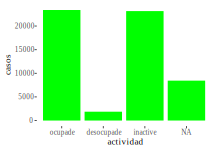
\includegraphics{EstadisticaParaCienciasSocialesConR_files/figure-latex/estadobarras-1} 

}

\caption{Condición laboral: frecuencias absolutas (barras adyacentes).}\label{fig:estadobarras}
\end{figure}

La categoría NA (not available) reúne a quienes no respondieron al cuestionario y a menores de 10 años, que no se les hace la pregunta. En el gráfico \ref{fig:apiladasabs}, se representa la misma información en barras apiladas.

\begin{figure}[H]

{\centering 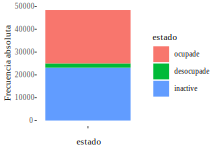
\includegraphics{EstadisticaParaCienciasSocialesConR_files/figure-latex/apiladasabs-1} 

}

\caption{Condición laboral: frecuencias absolutas (barras apiladas).}\label{fig:apiladasabs}
\end{figure}

En \ref{fig:apiladasrel}, se muestran, con el mismo tipo de representación, las frecuencias relativas.

\begin{figure}[H]

{\centering 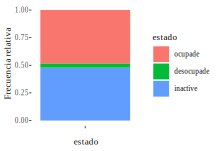
\includegraphics{EstadisticaParaCienciasSocialesConR_files/figure-latex/apiladasrel-1} 

}

\caption{Condición laboral: frecuencias relativas (barras apiladas).}\label{fig:apiladasrel}
\end{figure}

Para variables categóricas también se usa el \textbf{gráfico de sectores}, que se ilustra en \ref{fig:estadosectores}

\begin{figure}[H]

{\centering 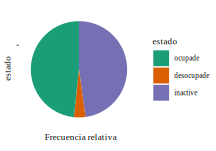
\includegraphics{EstadisticaParaCienciasSocialesConR_files/figure-latex/estadosectores-1} 

}

\caption{Condición laboral: frecuencias relativas (gráfico de sectores).}\label{fig:estadosectores}
\end{figure}

Este gráfico solo es adecuado cuando la variable tiene pocas categorías (no más de cuatro) y además cuando las frecuencias difieren sustancialmente. De lo contrario, resulta muy difícil apreciar diferencias entre ángulos, éstas son mucho más claras entre alturas de barras. La opción de agregar una leyenda con los porcentajes resuelve este problema, pero hace perder parte de la claridad visual del gráfico.

La representación gráfica de la tabla de frecuencias de variables cuantitativas (categorizadas), se llama \textbf{histograma}, se observa en \ref{fig:histedades}:

\begin{figure}[H]

{\centering 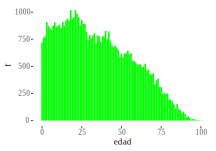
\includegraphics{EstadisticaParaCienciasSocialesConR_files/figure-latex/histedades-1} 

}

\caption{Histograma de edades.}\label{fig:histedades}
\end{figure}

El ancho de los rectángulos es la amplitud de las categorías que resultan de la categorización. Esta siempre se realiza con el criterio de intervalos iguales, que puede regularse, por ejemplo, si se toman intervalos de 5 años, el histograma queda como en el gráfico \ref{fig:histedadcinco}.

\begin{figure}[H]

{\centering 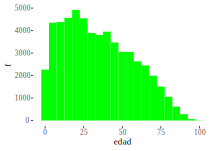
\includegraphics{EstadisticaParaCienciasSocialesConR_files/figure-latex/histedadcinco-1} 

}

\caption{Histograma de edades: categorías de 5 años.}\label{fig:histedadcinco}
\end{figure}

Cuando estos rectángulos se unen en sus puntos medios por una poligonal, resulta el \textbf{polígono de frecuencias} del gráfico \ref{fig:poligon}:

\begin{figure}[H]

{\centering 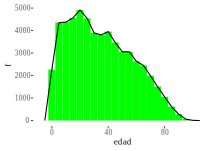
\includegraphics{EstadisticaParaCienciasSocialesConR_files/figure-latex/poligon-1} 

}

\caption{Polígono de frecuencias de las edades sobre el histograma.}\label{fig:poligon}
\end{figure}

Al polígono le fueron agregados dos intervalos, uno anterior al primero y uno posterior al último, cuyas frecuencias son cero, con el objetivo de ``cerrar'' el polígono sobre el eje horizontal.
El área que queda bajo este polígono es igual a la que encierran los rectángulos del histograma, y valdrá \(n\) si se grafican frecuencias absolutas ó \(1\) si son las relativas.\\
Cuando se muestra solo el polígono (gráfico \ref{fig:solopoli}), se tiene una representación simplificada de la distribución, que sirve para apreciar aspectos que se verán más adelante: forma, dispersión, simetría, etc. Además es preferible presentar en el eje vertical, frecuencias relativas antes que absolutas, para facilitar las comparaciones.

\begin{figure}[H]

{\centering 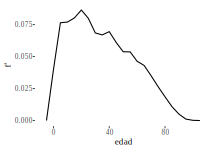
\includegraphics{EstadisticaParaCienciasSocialesConR_files/figure-latex/solopoli-1} 

}

\caption{Polígono de frecuencias de las edades.}\label{fig:solopoli}
\end{figure}

En variables cuantitativas es posible calcular frecuencias acumuladas, por lo que también ellas pueden representarse gráficamente. Si la variable es discreta, el gráfico se llama \textbf{gráfico de escalones}, cada valor aporta su frecuencia, que ``salta'' en el valor siguiente, por eso el gráfico tiene forma escalonada. Con la variable edad (CH06) de la EPH el gráfico de escalones es el de \ref{fig:escalones}.

\begin{figure}[H]

{\centering 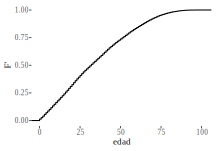
\includegraphics{EstadisticaParaCienciasSocialesConR_files/figure-latex/escalones-1} 

}

\caption{Ojiva de las edades.}\label{fig:escalones}
\end{figure}

En el que el eje horizontal se indican los valores de la variable discreta edad y en el vertical las frecuencias acumuladas de cada categoría (de cada valor discreto).\\
Si la variable es continua, se trata de la \textbf{ojiva de Galton}, las frecuencias se van acumulando gradualmente a medida que aumenta el valor de la variable. El gráfico \ref{fig:ojivabayley} muestra las frecuencias acumuladas de los pesos al nacer de un conjunto grande de niños y niñas que fueron evaluados con la prueba de Bayley:

\begin{figure}[H]

{\centering 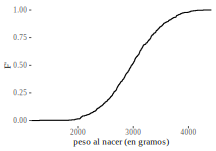
\includegraphics{EstadisticaParaCienciasSocialesConR_files/figure-latex/ojivabayley-1} 

}

\caption{Ojiva de los pesos al nacer.}\label{fig:ojivabayley}
\end{figure}

Debido a que en la práctica las variables nunca son continuas, siempre habrá ``escalones'' cuyo tamaño es el de la mínima medición posible de la variable (la apreciación del instrumento con que se mide).\\
La ojiva de Galton tiene otra virtud además de la claridad visual, ya que permite interpolar valores no observados, o que no aparecen en la tabla. Así, con el gráfico podemos responder a la pregunta ¿Qué proporción nación con 2512 g o menos? La respuesta consiste en buscar el valor 2512 gramos en el eje x, e identificar la frecuencia acumulada que le corresponde, como se muestra en \ref{fig:estimaacumulada}.

\begin{figure}[H]

{\centering 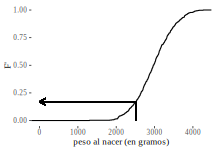
\includegraphics{EstadisticaParaCienciasSocialesConR_files/figure-latex/estimaacumulada-1} 

}

\caption{Estimación de la frecuencia acumulada para un valor del peso al nacer.}\label{fig:estimaacumulada}
\end{figure}

En este ejemplo, la ordenada (valor en el eje vertical) correspondiente a los 2512 gramos es aproximadamente \(0.17\), este resultado se lee diciendo que, de esta muestra, el \(17\%\) de quienes se sometieron a la evaluación nació con 2512 gramos o menos. En los capítulos siguientes veremos otras aplicaciones útiles de este procedimiento.\\
Además, el establecimiento de los límites de los intervalos según el criterio proporcional, puede realizarse en base a este gráfico. Según cuántos intervalos se quiera construir, se ubican los puntos correspondientes a las frecuencias acumuladas en el eje vertical y se buscan los valores de la variable (eje horizontal), que delimitan los intervalos. Por ejemplo, para cuatro intervalos, cada uno debe contener aproximadamente el 25\% de los casos, que corresponden a las frecuencias acumuladas de 25, 50 y 75\%. En el gráfico \ref{fig:cortacuatro} se ilustra el procedimiento; partiendo de las frecuencias acumuladas en el eje vertical, que son los valores de \({F}'\) de \(0.25\), \(0.50\) y \(0.75\), se buscan los valores de la variable en el horizontal.

\begin{figure}[H]

{\centering 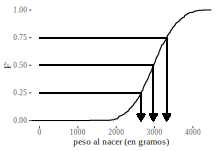
\includegraphics{EstadisticaParaCienciasSocialesConR_files/figure-latex/cortacuatro-1} 

}

\caption{Identificación de los valores de la variable para determinadas frecuencias acumuladas.}\label{fig:cortacuatro}
\end{figure}

Los valores hallados corresponden a 2646, 2968 y 3320 gramos. Que quiere decir que un cuarto nació con pesos entre el mínimo y 2646, otro cuarto pesó entre 2646 y 2968 gramos, y así con el resto. La distribución de frecuencias de esta variable así categorizada resulta:

\begin{longtable}[]{@{}lc@{}}
\caption{\label{tab:unnamed-chunk-112}Distribución de los pesos al nacer categorizados en cuatro intervalos proporcionales.}\tabularnewline
\toprule\noalign{}
Peso.nacCat & f \\
\midrule\noalign{}
\endfirsthead
\toprule\noalign{}
Peso.nacCat & f \\
\midrule\noalign{}
\endhead
\bottomrule\noalign{}
\endlastfoot
(1302.5,2646.5{]} & 113 \\
(2646.5,2967.5{]} & 113 \\
(2967.5,3319.8{]} & 113 \\
(3319.8,4268.5{]} & 114 \\
\end{longtable}

\pagebreak

\section{Hacerlo en R}\label{hacerlo-en-r-1}

Volvemos a leer la base que se trabajó en el capítulo anterior:

\begin{Shaded}
\begin{Highlighting}[]
\NormalTok{base.ejemplo }\OtherTok{\textless{}{-}} \FunctionTok{read.table}\NormalTok{(}\StringTok{"bases/archivostxt/base2019.txt"}\NormalTok{,}
  \AttributeTok{header =} \ConstantTok{TRUE}\NormalTok{, }\AttributeTok{sep =} \StringTok{" "}\NormalTok{, }\AttributeTok{na.strings =} \StringTok{"999"}
\NormalTok{)}
\end{Highlighting}
\end{Shaded}

Y repetimos las operaciones anteriores, de dar nombre a las variables, y de transformar en factor y etiquetar las variables que corresponda (para esto alcanza con copiar y pegar las instrucciones del capítulo anterior):

\begin{Shaded}
\begin{Highlighting}[]
\CommentTok{\# nombres de columnas:}
\FunctionTok{names}\NormalTok{(base.ejemplo) }\OtherTok{\textless{}{-}} \FunctionTok{c}\NormalTok{(}
  \StringTok{"caso"}\NormalTok{, }\StringTok{"grupo"}\NormalTok{, }\StringTok{"n.cuest"}\NormalTok{, }\StringTok{"nombre"}\NormalTok{, }\StringTok{"sexo"}\NormalTok{, }\StringTok{"genero"}\NormalTok{,}
  \StringTok{"edad"}\NormalTok{, }\StringTok{"acceso.redes"}\NormalTok{, }\StringTok{"red.usada"}\NormalTok{, }\StringTok{"red.otra"}\NormalTok{,}
  \StringTok{"tiempo.red"}\NormalTok{, }\StringTok{"con.q.vive"}\NormalTok{, }\StringTok{"relacion.otres"}\NormalTok{,}
  \StringTok{"q.aporta"}\NormalTok{, }\StringTok{"q.aporta.amigues"}\NormalTok{, }\StringTok{"edad.partida"}\NormalTok{,}
  \StringTok{"razon.partida"}\NormalTok{,}
  \StringTok{"razon.partida.otra"}\NormalTok{, }\StringTok{"calidad.sueño"}\NormalTok{,}
  \StringTok{"preocupacion"}\NormalTok{, }\StringTok{"golpeo"}\NormalTok{, }\StringTok{"robo"}\NormalTok{, }\StringTok{"cuanto.da"}\NormalTok{, }\StringTok{"comision"}
\NormalTok{)}

\CommentTok{\# transformar en factor y etiquetar las nominales:}
\NormalTok{base.ejemplo}\SpecialCharTok{$}\NormalTok{sexo }\OtherTok{\textless{}{-}} \FunctionTok{as.factor}\NormalTok{(base.ejemplo}\SpecialCharTok{$}\NormalTok{sexo)}
\FunctionTok{levels}\NormalTok{(base.ejemplo}\SpecialCharTok{$}\NormalTok{sexo) }\OtherTok{\textless{}{-}} \FunctionTok{c}\NormalTok{(}\StringTok{"varones"}\NormalTok{, }\StringTok{"mujeres"}\NormalTok{)}

\NormalTok{base.ejemplo}\SpecialCharTok{$}\NormalTok{con.q.vive }\OtherTok{\textless{}{-}} \FunctionTok{as.factor}\NormalTok{(base.ejemplo}\SpecialCharTok{$}\NormalTok{con.q.vive)}
\FunctionTok{levels}\NormalTok{(base.ejemplo}\SpecialCharTok{$}\NormalTok{con.q.vive) }\OtherTok{\textless{}{-}} \FunctionTok{c}\NormalTok{(}
  \StringTok{"flia.origen"}\NormalTok{, }\StringTok{"flia.nueva"}\NormalTok{,}
  \StringTok{"hermanes.o.amigues"}\NormalTok{, }\StringTok{"solo"}\NormalTok{,}
  \StringTok{"con.otres"}
\NormalTok{)}

\NormalTok{base.ejemplo}\SpecialCharTok{$}\NormalTok{q.aporta }\OtherTok{\textless{}{-}} \FunctionTok{as.factor}\NormalTok{(base.ejemplo}\SpecialCharTok{$}\NormalTok{q.aporta)}
\FunctionTok{levels}\NormalTok{(base.ejemplo}\SpecialCharTok{$}\NormalTok{q.aporta) }\OtherTok{\textless{}{-}} \FunctionTok{c}\NormalTok{(}
  \StringTok{"si.misme"}\NormalTok{, }\StringTok{"flia.origen"}\NormalTok{,}
  \StringTok{"flia.nueva"}\NormalTok{, }\StringTok{"entre.amigues"}
\NormalTok{)}

\NormalTok{base.ejemplo}\SpecialCharTok{$}\NormalTok{acceso.redes }\OtherTok{\textless{}{-}} \FunctionTok{as.factor}\NormalTok{(base.ejemplo}\SpecialCharTok{$}\NormalTok{acceso.redes)}
\FunctionTok{levels}\NormalTok{(base.ejemplo}\SpecialCharTok{$}\NormalTok{acceso.redes) }\OtherTok{\textless{}{-}} \FunctionTok{c}\NormalTok{(}\StringTok{"si"}\NormalTok{, }\StringTok{"no"}\NormalTok{)}

\NormalTok{base.ejemplo}\SpecialCharTok{$}\NormalTok{red.usada }\OtherTok{\textless{}{-}} \FunctionTok{as.factor}\NormalTok{(base.ejemplo}\SpecialCharTok{$}\NormalTok{red.usada)}
\FunctionTok{levels}\NormalTok{(base.ejemplo}\SpecialCharTok{$}\NormalTok{red.usada) }\OtherTok{\textless{}{-}} \FunctionTok{c}\NormalTok{(}
  \StringTok{"Instagram"}\NormalTok{, }\StringTok{"Facebook"}\NormalTok{, }\StringTok{"Twitter"}\NormalTok{,}
  \StringTok{"Linkedin"}\NormalTok{, }\StringTok{"Tinder/Grindr/happn"}\NormalTok{,}
  \StringTok{"Snapchat"}\NormalTok{, }\StringTok{"Ninguna"}\NormalTok{, }\StringTok{"Otra"}
\NormalTok{)}

\NormalTok{base.ejemplo}\SpecialCharTok{$}\NormalTok{razon.partida }\OtherTok{\textless{}{-}} \FunctionTok{as.factor}\NormalTok{(}
\NormalTok{  base.ejemplo}\SpecialCharTok{$}\NormalTok{razon.partida}
\NormalTok{)}
\FunctionTok{levels}\NormalTok{(base.ejemplo}\SpecialCharTok{$}\NormalTok{razon.partida) }\OtherTok{\textless{}{-}} \FunctionTok{c}\NormalTok{(}
  \StringTok{"estudio"}\NormalTok{, }\StringTok{"nueva.flia"}\NormalTok{, }\StringTok{"ganas"}\NormalTok{, }\StringTok{"otras"}
\NormalTok{)}
\end{Highlighting}
\end{Shaded}

\subsection{Tablas univariadas}\label{tablas-univariadas}

Las tablas de distribución de frecuencias se solicitan con un comando del paquete \{base\} que se llama \texttt{table}, que tiene como argumento la variable cuya tabla se pide. Recordemos que para hacer referencia a una variable, se debe indicar el nombre de la matriz de datos de donde proviene, seguida del signo pesos y luego el nombre de la variable. Así, para la tabla de distribución de frecuencias de la variable sexo:

\begin{Shaded}
\begin{Highlighting}[]
\FunctionTok{table}\NormalTok{(base.ejemplo}\SpecialCharTok{$}\NormalTok{sexo)}
\end{Highlighting}
\end{Shaded}

\begin{verbatim}
## 
## varones mujeres 
##    2240    2755
\end{verbatim}

Para ``quien aporta'':

\begin{Shaded}
\begin{Highlighting}[]
\FunctionTok{table}\NormalTok{(base.ejemplo}\SpecialCharTok{$}\NormalTok{q.aporta)}
\end{Highlighting}
\end{Shaded}

\begin{verbatim}
## 
##      si.misme   flia.origen    flia.nueva entre.amigues 
##           974          2692           456           422
\end{verbatim}

Por defecto, este comando descarta los casos perdidos (los NA). Si se los quiere ver, hay que pedirlo expresamente:

\begin{Shaded}
\begin{Highlighting}[]
\FunctionTok{table}\NormalTok{(base.ejemplo}\SpecialCharTok{$}\NormalTok{q.aporta, }\AttributeTok{useNA =} \StringTok{"always"}\NormalTok{)}
\end{Highlighting}
\end{Shaded}

\begin{verbatim}
## 
##      si.misme   flia.origen    flia.nueva entre.amigues          <NA> 
##           974          2692           456           422           459
\end{verbatim}

Las opciones de \texttt{useNA} son ``\(no\)'', que es la que se aplica por defecto, ``\(ifany\)'' (si hay alguno) y la que hemos usado en este ejemplo, ``\(always\)'' (siempre).

Existe un paquete especializado para descripciones estadísticas, llamado \{summarytools\} que contiene herramientas que simplifican operaciones y ofrecen una presentación más familiar de las tablas. Primero se lo debe instalar:

\begin{Shaded}
\begin{Highlighting}[]
\FunctionTok{install.packages}\NormalTok{(}\StringTok{"summarytools"}\NormalTok{)}
\end{Highlighting}
\end{Shaded}

Y cargarlo en la sesión:

\begin{Shaded}
\begin{Highlighting}[]
\FunctionTok{library}\NormalTok{(}\StringTok{"summarytools"}\NormalTok{)}
\end{Highlighting}
\end{Shaded}

En este paquete, el comando para pedir una tabla es \texttt{freq}. Para la misma variable anterior:

\begin{Shaded}
\begin{Highlighting}[]
\FunctionTok{freq}\NormalTok{(base.ejemplo}\SpecialCharTok{$}\NormalTok{q.aporta)}
\end{Highlighting}
\end{Shaded}

\begin{verbatim}
## Frequencies  
## base.ejemplo$q.aporta  
## Type: Factor  
## 
##                       Freq   % Valid   % Valid Cum.   % Total   % Total Cum.
## ------------------- ------ --------- -------------- --------- --------------
##            si.misme    974     21.43          21.43     19.47          19.47
##         flia.origen   2692     59.24          80.68     53.81          73.28
##          flia.nueva    456     10.04          90.71      9.11          82.39
##       entre.amigues    422      9.29         100.00      8.43          90.83
##                <NA>    459                               9.17         100.00
##               Total   5003    100.00         100.00    100.00         100.00
\end{verbatim}

La diferencia entre frecuencias válidas y totales es que las primeras descuentan los casos perdidos (NA). Si bien la tabla tiene ahora mejor aspecto, las columnas 3 y 5 (correspondientes a frecuencias acumuladas), no pueden interpretarse, porque esta variable no admite frecuencias acumuladas, que este comando calcula por defecto. Puede solicitarse expresamente que no lo haga:

\begin{Shaded}
\begin{Highlighting}[]
\FunctionTok{freq}\NormalTok{(base.ejemplo}\SpecialCharTok{$}\NormalTok{q.aporta, }\AttributeTok{cumul =} \ConstantTok{FALSE}\NormalTok{)}
\end{Highlighting}
\end{Shaded}

\begin{verbatim}
## Frequencies  
## base.ejemplo$q.aporta  
## Type: Factor  
## 
##                       Freq   % Valid   % Total
## ------------------- ------ --------- ---------
##            si.misme    974     21.43     19.47
##         flia.origen   2692     59.24     53.81
##          flia.nueva    456     10.04      9.11
##       entre.amigues    422      9.29      8.43
##                <NA>    459                9.17
##               Total   5003    100.00    100.00
\end{verbatim}

Y se obtienen frecuencias absolutas y relativas, estas últimas respecto de los casos válidos y respecto del total de casos.\\
Si la variable es ordinal, las frecuencias acumuladas sí admiten interpretación. Para la variable ``ocasión en que golpeó a alguien'', tenemos:

\begin{Shaded}
\begin{Highlighting}[]
\FunctionTok{freq}\NormalTok{(base.ejemplo}\SpecialCharTok{$}\NormalTok{golpeo)}
\end{Highlighting}
\end{Shaded}

\begin{verbatim}
## Frequencies  
## base.ejemplo$golpeo  
## Type: Integer  
## 
##               Freq   % Valid   % Valid Cum.   % Total   % Total Cum.
## ----------- ------ --------- -------------- --------- --------------
##           1   4180     83.62          83.62     83.55          83.55
##           2    535     10.70          94.32     10.69          94.24
##           3    211      4.22          98.54      4.22          98.46
##           4     46      0.92          99.46      0.92          99.38
##           5     21      0.42          99.88      0.42          99.80
##           6      2      0.04          99.92      0.04          99.84
##           7      3      0.06          99.98      0.06          99.90
##           8      1      0.02         100.00      0.02          99.92
##        <NA>      4                               0.08         100.00
##       Total   5003    100.00         100.00    100.00         100.00
\end{verbatim}

La salida se puede simplificar si no hay interés en un análisis puntual sobre los casos perdidos, eliminando su aparición. En el comando \texttt{freq}, el argumento \texttt{report.nas=FALSE} establece que se elimine la referencia a los casos perdidos, ya que aun cuando no haya, la tabla los menciona, con frecuencia cero.

\begin{Shaded}
\begin{Highlighting}[]
\FunctionTok{freq}\NormalTok{(base.ejemplo}\SpecialCharTok{$}\NormalTok{golpeo, }\AttributeTok{report.nas =} \ConstantTok{FALSE}\NormalTok{)}
\end{Highlighting}
\end{Shaded}

\begin{verbatim}
## Frequencies  
## base.ejemplo$golpeo  
## Type: Integer  
## 
##               Freq        %   % Cum.
## ----------- ------ -------- --------
##           1   4180    83.62    83.62
##           2    535    10.70    94.32
##           3    211     4.22    98.54
##           4     46     0.92    99.46
##           5     21     0.42    99.88
##           6      2     0.04    99.92
##           7      3     0.06    99.98
##           8      1     0.02   100.00
##       Total   4999   100.00   100.00
\end{verbatim}

Que es la versión más familiar de la tabla. con frecuencias absolutas, relativas simples y acumuladas y ya no hay mención a válidos o totales, porque solo están presentes los válidos.

\subsection{Recategorización}\label{recategorizaciuxf3n-1}

La construcción de categorías a partir de una variable continua, se realiza con el comando \texttt{cut}, cuyo argumento contiene a la variable que se va a recategorizar, y una instrucción \texttt{breaks=} que especifica el modo de hacer los cortes, esta instrucción difiere según los tipos de recategorización.\\
Para ver los comandos, vamos a generar nuevas variables en la base, que se llaman edad4i, edad4p y edad4t (edad en cuatro categorías, con criterio de amplitud igual, proporcional y teórica), y definimos esas categorías de las tres maneras diferentes que se han visto. Antes de eso vamos a eliminar de la base los casos que no tengan información en la variable edad. El modo de hacerlo es redefinir el data frame base.ejemplo, como un subconjunto de él que solo contenga los casos para los cuales la variable edad no es NA:

\begin{Shaded}
\begin{Highlighting}[]
\NormalTok{base.ejemplo }\OtherTok{\textless{}{-}} \FunctionTok{subset}\NormalTok{(}
\NormalTok{  base.ejemplo,}
  \FunctionTok{is.na}\NormalTok{(base.ejemplo}\SpecialCharTok{$}\NormalTok{edad) }\SpecialCharTok{==} \ConstantTok{FALSE}
\NormalTok{)}
\end{Highlighting}
\end{Shaded}

Ahora la base tiene 4991 observaciones, como se ve en el panel superior derecho.

\subsubsection{Intervalos de amplitud igual}\label{intervalos-de-amplitud-igual-1}

Para que los intervalos sean iguales, en el argumento \texttt{breaks} solo se indica la cantidad de ellos que se quiere, en este caso, cuatro:

\begin{Shaded}
\begin{Highlighting}[]
\NormalTok{base.ejemplo}\SpecialCharTok{$}\NormalTok{edad4i }\OtherTok{\textless{}{-}} \FunctionTok{cut}\NormalTok{(base.ejemplo}\SpecialCharTok{$}\NormalTok{edad, }\AttributeTok{breaks =} \DecValTok{4}\NormalTok{)}
\end{Highlighting}
\end{Shaded}

Y pedimos una tabla:

\begin{Shaded}
\begin{Highlighting}[]
\FunctionTok{freq}\NormalTok{(base.ejemplo}\SpecialCharTok{$}\NormalTok{edad4i, }\AttributeTok{report.nas =} \ConstantTok{FALSE}\NormalTok{)}
\end{Highlighting}
\end{Shaded}

\begin{verbatim}
## Frequencies  
## base.ejemplo$edad4i  
## Type: Factor  
## 
##                 Freq        %   % Cum.
## ------------- ------ -------- --------
##       (15,27]   4027    80.69    80.69
##       (27,39]    954    19.11    99.80
##       (39,51]      4     0.08    99.88
##       (51,63]      6     0.12   100.00
##         Total   4991   100.00   100.00
\end{verbatim}

Los intervalos se presentan con un paréntesis a la izquierda y un corchete a la derecha, lo que indica que los intervalos son abiertos a la izquierda y cerrados a la derecha, incluyen al límite superior y excluyen al inferior. Por ejemplo las personas con edad 27 años están contadas en el primer intervalo y no en el segundo, aunque el 27 aparezca en ambos.

\subsubsection{Intervalos de amplitud proporcional}\label{intervalos-de-amplitud-proporcional-1}

Para lograr que cada intervalo tenga aproximadamente la misma proporción de casos, primero hay que saber cuál es esa proporción. En este ejemplo, son cuatro intervalos, por lo que un cuarto de los casos debe estar en cada uno, es decir el 25\%. En el próximo capítulo se definirán medidas resumen que marcan estos puntos de corte, se denominan cuantiles. Para este ejemplo, hay que cortar el campo de variación en los valores de la variable que acumulen 25\%, 50\% y 75\%, de modo que entre cada par de ellos quede 25\% de casos. Esos números se llaman cuantiles 0.25, 0.50 y 0.75. En el argumento \texttt{breaks} se indican, concatenados, cada uno de los límites de los intervalos desde el mínimo valor de la variable (\texttt{min()}), los cuantiles .25, .50 y .75 y finalmente el máximo (\texttt{max()}):

\begin{Shaded}
\begin{Highlighting}[]
\NormalTok{base.ejemplo}\SpecialCharTok{$}\NormalTok{edad4p }\OtherTok{\textless{}{-}} \FunctionTok{cut}\NormalTok{(base.ejemplo}\SpecialCharTok{$}\NormalTok{edad,}
  \AttributeTok{breaks =} \FunctionTok{c}\NormalTok{(}
    \FunctionTok{min}\NormalTok{(base.ejemplo}\SpecialCharTok{$}\NormalTok{edad), }\CommentTok{\# inicio}
    \FunctionTok{quantile}\NormalTok{(base.ejemplo}\SpecialCharTok{$}\NormalTok{edad, .}\DecValTok{25}\NormalTok{), }\CommentTok{\# primer corte: 25\% acumulado}
    \FunctionTok{quantile}\NormalTok{(base.ejemplo}\SpecialCharTok{$}\NormalTok{edad, .}\DecValTok{50}\NormalTok{), }\CommentTok{\# segundo corte: 50\% acumulado}
    \FunctionTok{quantile}\NormalTok{(base.ejemplo}\SpecialCharTok{$}\NormalTok{edad, .}\DecValTok{75}\NormalTok{), }\CommentTok{\# tercer corte: 75\% acumulado}
    \FunctionTok{max}\NormalTok{(base.ejemplo}\SpecialCharTok{$}\NormalTok{edad) }\CommentTok{\# fin}
\NormalTok{  )}
\NormalTok{)}
\end{Highlighting}
\end{Shaded}

La tabla es:

\begin{verbatim}
## Frequencies  
## base.ejemplo$edad4p  
## Type: Factor  
## 
##                 Freq        %   % Cum.
## ------------- ------ -------- --------
##       (15,19]   1694    33.95    33.95
##       (19,21]    973    19.50    53.45
##       (21,26]   1206    24.17    77.62
##       (26,63]   1117    22.38   100.00
##         Total   4990   100.00   100.00
\end{verbatim}

Como se trata de una variable discreta, la aproximación del 25\% en cada intervalo no es muy cercana. En este ejemplo sucede que la edad 18 años tiene muchos casos, por lo que incluirla en el primer intervalo o en el segundo, cambia mucho la proporción de casos que quedan dentro del intervalo.

\subsubsection{Intervalos de amplitud teórica}\label{intervalos-de-amplitud-teuxf3rica-1}

De mismo modo que antes, se indica al argumento \texttt{breaks}, la concatenación de los puntos de corte, solo que éstos se establecen de antemano, por ejemplo, para hacer grupos 15-18, 19-23, 24-35 y 36 en adelante, pedimos:

\begin{Shaded}
\begin{Highlighting}[]
\NormalTok{base.ejemplo}\SpecialCharTok{$}\NormalTok{edad4t }\OtherTok{\textless{}{-}} \FunctionTok{cut}\NormalTok{(base.ejemplo}\SpecialCharTok{$}\NormalTok{edad,}
  \AttributeTok{breaks =} \FunctionTok{c}\NormalTok{(}
    \FunctionTok{min}\NormalTok{(base.ejemplo}\SpecialCharTok{$}\NormalTok{edad), }\DecValTok{18}\NormalTok{,}
    \DecValTok{23}\NormalTok{, }\DecValTok{35}\NormalTok{, }\FunctionTok{max}\NormalTok{(base.ejemplo}\SpecialCharTok{$}\NormalTok{edad)}
\NormalTok{  )}
\NormalTok{)}
\end{Highlighting}
\end{Shaded}

La tabla resulta:

\begin{Shaded}
\begin{Highlighting}[]
\FunctionTok{freq}\NormalTok{(base.ejemplo}\SpecialCharTok{$}\NormalTok{edad4t, }\AttributeTok{report.nas =} \ConstantTok{FALSE}\NormalTok{)}
\end{Highlighting}
\end{Shaded}

\begin{verbatim}
## Frequencies  
## base.ejemplo$edad4t  
## Type: Factor  
## 
##                 Freq        %   % Cum.
## ------------- ------ -------- --------
##       (15,18]   1013    20.30    20.30
##       (18,23]   2276    45.61    65.91
##       (23,35]   1684    33.75    99.66
##       (35,63]     17     0.34   100.00
##         Total   4990   100.00   100.00
\end{verbatim}

\subsection{Representaciones gráficas}\label{representaciones-gruxe1ficas}

El paquete \{base\} contiene rutinas elementales de graficación, sin embargo, desde aquí vamos a empezar a usar un paquete específico para eso; \texttt{ggplot2}, que debe instalarse

\begin{Shaded}
\begin{Highlighting}[]
\FunctionTok{install.packages}\NormalTok{(}\StringTok{"ggplot2"}\NormalTok{)}
\end{Highlighting}
\end{Shaded}

y cargarse en la sesión

\begin{Shaded}
\begin{Highlighting}[]
\FunctionTok{library}\NormalTok{(}\StringTok{"ggplot2"}\NormalTok{)}
\end{Highlighting}
\end{Shaded}

La construcción de los gráficos en \texttt{ggplot} se hace por medio de capas que se van agregando. Las capas tienen cinco componentes:

\begin{itemize}
\tightlist
\item
  Los datos, que es la base de donde provienen la variables que se van a graficar. Si más tarde se grafica lo mismo para otra base, solo se debe cambiar ese origen, lo mismo si la base se modifica.\\
\item
  Un conjunto de mapeos estéticos (\texttt{aes}), que describen el modo en que las variables de la base van a ser representadas en las propiedades estéticas de la capa. - El \texttt{geom}, que describe la figura geométrica que se va a usar para dibujar la capa.\\
\item
  La transformación estadística (\texttt{stat}) que opera sobre los datos originales para sintetizarlos de modo que se los pueda representar.\\
\item
  Los ajustes de posición
\end{itemize}

Cada figura geométrica (\texttt{geom}) tiene asociada una transformación estadística por defecto, por lo que no es necesario especificarla, salvo que se quiera modificar. Por ejemplo si los datos para un gráfico provienen de una matriz de datos (\texttt{data.frame}), la transformación consiste en contar las ocurrencias de cada valor, ese es el \texttt{stat} por defecto. Pero si se quiere graficar desde una tabla de distribución de frecuencias, entonces en lugar de contar las veces que aparece cada categoría, hay que considerar las frecuencias. En este último caso, será necesario especificar una transformación diferente.

\subsubsection{Creación de un gráfico}\label{creaciuxf3n-de-un-gruxe1fico}

La primera instrucción para crear un gráfico es \texttt{ggplot()}. Esta instrucción va a tener como argumento, la matriz de donde provienen las variables a graficar. Puede incluirse el mapeo estético también, pero en este ejemplo lo vamos a agregar en las capas que indican el tipo de gráfico.\\
Si se aplica ese comando a la base.ejemplo:

\begin{Shaded}
\begin{Highlighting}[]
\FunctionTok{ggplot}\NormalTok{(base.ejemplo) }\SpecialCharTok{+} \FunctionTok{theme\_gray}\NormalTok{(}\AttributeTok{base\_size =} \DecValTok{9}\NormalTok{)}
\end{Highlighting}
\end{Shaded}

\begin{center}
\includegraphics{EstadisticaParaCienciasSocialesConR_files/figure-latex/unnamed-chunk-133-1} \end{center}

El resultado son solo los ejes, no se ha indicado aun qué variables graficar ni qué tipo de gráfico hacer. Eso se especifica en las capas.\\
Para hacer un gráfico de barras, luego de indicar sobre qué base se va a trabajar, en el argumento de ggplot, se agrega una capa de barras (\texttt{geom\_bar}) con la variable que se va a representar (no hace falta indicar de qué matriz de datos proviene, eso ya está en el argumento de \texttt{ggplot}):

\begin{Shaded}
\begin{Highlighting}[]
\FunctionTok{ggplot}\NormalTok{(base.ejemplo) }\SpecialCharTok{+} \FunctionTok{geom\_bar}\NormalTok{(}\FunctionTok{aes}\NormalTok{(red.usada)) }\SpecialCharTok{+} \FunctionTok{theme\_gray}\NormalTok{(}\AttributeTok{base\_size =} \DecValTok{9}\NormalTok{)}
\end{Highlighting}
\end{Shaded}

\begin{center}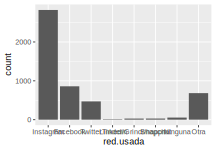
\includegraphics{EstadisticaParaCienciasSocialesConR_files/figure-latex/unnamed-chunk-134-1} \end{center}

Y vamos a mejorarlo en su aspecto. Para quitar los NA, tomamos como argumento de ggplot, no la base completa, sino un subconjunto que no tenga NA en esta variable:

\begin{Shaded}
\begin{Highlighting}[]
\FunctionTok{ggplot}\NormalTok{(}\FunctionTok{subset}\NormalTok{(base.ejemplo, }\FunctionTok{is.na}\NormalTok{(base.ejemplo}\SpecialCharTok{$}\NormalTok{red.usada) }\SpecialCharTok{==} \ConstantTok{FALSE}\NormalTok{)) }\SpecialCharTok{+}
  \FunctionTok{geom\_bar}\NormalTok{(}\FunctionTok{aes}\NormalTok{(red.usada)) }\SpecialCharTok{+} \FunctionTok{theme\_gray}\NormalTok{(}\AttributeTok{base\_size =} \DecValTok{9}\NormalTok{)}
\end{Highlighting}
\end{Shaded}

\begin{center}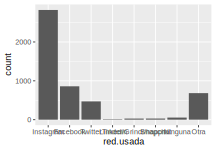
\includegraphics{EstadisticaParaCienciasSocialesConR_files/figure-latex/unnamed-chunk-135-1} \end{center}

Además de hacer el gráfico (ejecutar el comando) podemos guardarlo como un objeto, lo llamamos p1:

\begin{Shaded}
\begin{Highlighting}[]
\NormalTok{p1 }\OtherTok{\textless{}{-}} \FunctionTok{ggplot}\NormalTok{(}\FunctionTok{subset}\NormalTok{(base.ejemplo, }\FunctionTok{is.na}\NormalTok{(base.ejemplo}\SpecialCharTok{$}\NormalTok{red.usada) }\SpecialCharTok{==} \ConstantTok{FALSE}\NormalTok{)) }\SpecialCharTok{+}
  \FunctionTok{geom\_bar}\NormalTok{(}\FunctionTok{aes}\NormalTok{(red.usada)) }\SpecialCharTok{+}
  \FunctionTok{theme\_gray}\NormalTok{(}\AttributeTok{base\_size =} \DecValTok{9}\NormalTok{)}
\end{Highlighting}
\end{Shaded}

El objeto (de clase \texttt{ggplot}) aparece en el panel superior derecho. A las capas subsiguientes las agregamos sobre p1. Una capa de rótulos y se crea p2:

\begin{Shaded}
\begin{Highlighting}[]
\NormalTok{(p2 }\OtherTok{\textless{}{-}}\NormalTok{ p1 }\SpecialCharTok{+} \FunctionTok{xlab}\NormalTok{(}\StringTok{"Red más usada"}\NormalTok{) }\SpecialCharTok{+} \FunctionTok{ylab}\NormalTok{(}\StringTok{"cantidad de casos"}\NormalTok{))}
\end{Highlighting}
\end{Shaded}

\begin{center}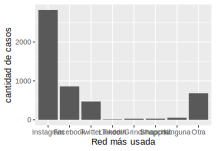
\includegraphics{EstadisticaParaCienciasSocialesConR_files/figure-latex/unnamed-chunk-137-1} \end{center}

El paréntesis que encierra toda la expresión se usa para que, al mismo tiempo que se defina el objeto p2, se ejecute el comando y se vea el gráfico.
Las etiquetas de los ejes se vuelven más legibles si se giran los ejes:

\begin{Shaded}
\begin{Highlighting}[]
\NormalTok{p2 }\SpecialCharTok{+} \FunctionTok{coord\_flip}\NormalTok{()}
\end{Highlighting}
\end{Shaded}

\begin{center}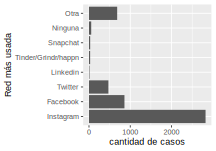
\includegraphics{EstadisticaParaCienciasSocialesConR_files/figure-latex/unnamed-chunk-138-1} \end{center}

Vamos a usar este ejemplo para ilustrar la diferencia entre ``fijar'' y ``mapear'' a un atributo estético, que en este caso será el color de relleno de las barras, con el comando \texttt{fill} (rellenar). Fijar el color es simplemente establecerlo como preferencia para todas las barras, es un argumento de la capa \texttt{geom\_bar}:

\begin{Shaded}
\begin{Highlighting}[]
\FunctionTok{ggplot}\NormalTok{(}\FunctionTok{subset}\NormalTok{(base.ejemplo, }\FunctionTok{is.na}\NormalTok{(base.ejemplo}\SpecialCharTok{$}\NormalTok{red.usada) }\SpecialCharTok{==} \ConstantTok{FALSE}\NormalTok{)) }\SpecialCharTok{+}
  \FunctionTok{geom\_bar}\NormalTok{(}\FunctionTok{aes}\NormalTok{(red.usada), }\AttributeTok{fill =} \StringTok{"green"}\NormalTok{) }\SpecialCharTok{+} \FunctionTok{coord\_flip}\NormalTok{()}
\end{Highlighting}
\end{Shaded}

\begin{center}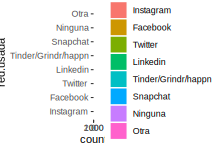
\includegraphics{EstadisticaParaCienciasSocialesConR_files/figure-latex/unnamed-chunk-139-1} \end{center}

Por el contrario, ``mapear'' es pedir que el color de relleno cambie en base a las categorías de una variable que se especifica, éste es un argumento de \texttt{aes}. Solo para ver los efectos, lo usamos con la misma variable que se representa en el eje:

\begin{Shaded}
\begin{Highlighting}[]
\FunctionTok{ggplot}\NormalTok{(}\FunctionTok{subset}\NormalTok{(base.ejemplo, }\FunctionTok{is.na}\NormalTok{(base.ejemplo}\SpecialCharTok{$}\NormalTok{red.usada) }\SpecialCharTok{==} \ConstantTok{FALSE}\NormalTok{)) }\SpecialCharTok{+}
  \FunctionTok{geom\_bar}\NormalTok{(}\FunctionTok{aes}\NormalTok{(red.usada, }\AttributeTok{fill =}\NormalTok{ red.usada)) }\SpecialCharTok{+} \FunctionTok{coord\_flip}\NormalTok{()}
\end{Highlighting}
\end{Shaded}

\begin{center}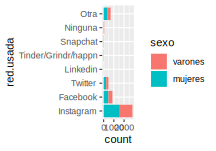
\includegraphics{EstadisticaParaCienciasSocialesConR_files/figure-latex/unnamed-chunk-140-1} \end{center}

Y en el gráfico el cambio se ve en que se usó un color para cada categoría de red.usada.

Dos diferencias importantes en la sintaxis:\\
- el comando \texttt{fill} va dentro de \texttt{aes} cuando se mapea y fuera cuando se fija\\
- el color fijo (green en este ejemplo) va entre comillas, el nombre de la variable, no.

En este ejemplo, el mapeo no aporta ninguna información nueva, ya que el nombre de la red está en el eje. Sin embargo, el mapeo es muy útil para introducir otra variable y ver las diferencias, por ejemplo, para observar la diferencia en la preferencia de redes según sexo. Para hacerlo, se recorta la matriz de datos y se retienen solo los casos que no sean NA en red.usada ni tampoco en sexo. Para que se cumplan las dos condiciones indicamos la conjunción \(y\), con el símbolo \(\&\):

\begin{Shaded}
\begin{Highlighting}[]
\FunctionTok{ggplot}\NormalTok{(}\FunctionTok{subset}\NormalTok{(}
\NormalTok{  base.ejemplo, }\FunctionTok{is.na}\NormalTok{(}
\NormalTok{    base.ejemplo}\SpecialCharTok{$}\NormalTok{red.usada}
\NormalTok{  ) }\SpecialCharTok{==} \ConstantTok{FALSE} \SpecialCharTok{\&} \FunctionTok{is.na}\NormalTok{(}
\NormalTok{    base.ejemplo}\SpecialCharTok{$}\NormalTok{sexo}
\NormalTok{  ) }\SpecialCharTok{==} \ConstantTok{FALSE}
\NormalTok{)) }\SpecialCharTok{+}
  \FunctionTok{geom\_bar}\NormalTok{(}\FunctionTok{aes}\NormalTok{(red.usada, }\AttributeTok{fill =}\NormalTok{ sexo)) }\SpecialCharTok{+} \FunctionTok{coord\_flip}\NormalTok{()}
\end{Highlighting}
\end{Shaded}

\begin{center}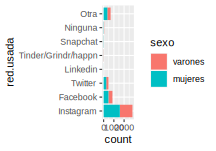
\includegraphics{EstadisticaParaCienciasSocialesConR_files/figure-latex/unnamed-chunk-141-1} \end{center}

Aquí vemos que la preferencia por redes está bastante equilibrada entre mujeres y varones.

El histograma tiene su propia capa, \texttt{geom\_histogram}. Para el caso de la variable edad:

\begin{Shaded}
\begin{Highlighting}[]
\FunctionTok{ggplot}\NormalTok{(base.ejemplo) }\SpecialCharTok{+}
  \FunctionTok{geom\_histogram}\NormalTok{(}\FunctionTok{aes}\NormalTok{(edad))}
\end{Highlighting}
\end{Shaded}

\begin{center}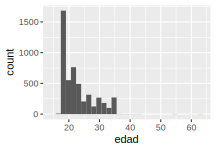
\includegraphics{EstadisticaParaCienciasSocialesConR_files/figure-latex/unnamed-chunk-142-1} \end{center}

Por defecto, se generan 30 intervalos, lo cual puede ajustarse, por ejemplo, a 15:

\begin{Shaded}
\begin{Highlighting}[]
\FunctionTok{ggplot}\NormalTok{(base.ejemplo) }\SpecialCharTok{+}
  \FunctionTok{geom\_histogram}\NormalTok{(}\FunctionTok{aes}\NormalTok{(edad), }\AttributeTok{bins =} \DecValTok{15}\NormalTok{)}
\end{Highlighting}
\end{Shaded}

\begin{center}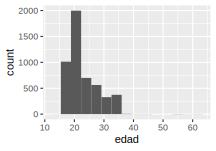
\includegraphics{EstadisticaParaCienciasSocialesConR_files/figure-latex/unnamed-chunk-143-1} \end{center}

Las opciones de mapeo son como con \texttt{geom\_bar}:

\begin{Shaded}
\begin{Highlighting}[]
\FunctionTok{ggplot}\NormalTok{(}\FunctionTok{subset}\NormalTok{(}
\NormalTok{  base.ejemplo,}
  \FunctionTok{is.na}\NormalTok{(base.ejemplo}\SpecialCharTok{$}\NormalTok{sexo) }\SpecialCharTok{==} \ConstantTok{FALSE}
\NormalTok{)) }\SpecialCharTok{+}
  \FunctionTok{geom\_histogram}\NormalTok{(}\FunctionTok{aes}\NormalTok{(edad, }\AttributeTok{fill =}\NormalTok{ sexo), }\AttributeTok{bins =} \DecValTok{15}\NormalTok{)}
\end{Highlighting}
\end{Shaded}

\begin{center}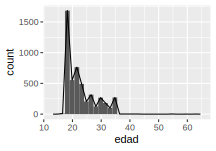
\includegraphics{EstadisticaParaCienciasSocialesConR_files/figure-latex/unnamed-chunk-144-1} \end{center}

El polígono de frecuencias es una capa que se agrega al histograma:

\begin{Shaded}
\begin{Highlighting}[]
\FunctionTok{ggplot}\NormalTok{(base.ejemplo) }\SpecialCharTok{+}
  \FunctionTok{geom\_histogram}\NormalTok{(}\FunctionTok{aes}\NormalTok{(edad)) }\SpecialCharTok{+}
  \FunctionTok{geom\_freqpoly}\NormalTok{(}\FunctionTok{aes}\NormalTok{(edad))}
\end{Highlighting}
\end{Shaded}

\begin{center}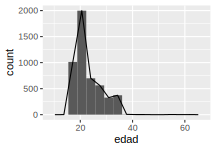
\includegraphics{EstadisticaParaCienciasSocialesConR_files/figure-latex/unnamed-chunk-145-1} \end{center}

Si se quiere ajustar el número de intervalos, conviene hacerlo igual en las dos capas:

\begin{Shaded}
\begin{Highlighting}[]
\FunctionTok{ggplot}\NormalTok{(base.ejemplo) }\SpecialCharTok{+}
  \FunctionTok{geom\_histogram}\NormalTok{(}\FunctionTok{aes}\NormalTok{(edad), }\AttributeTok{bins =} \DecValTok{15}\NormalTok{) }\SpecialCharTok{+}
  \FunctionTok{geom\_freqpoly}\NormalTok{(}\FunctionTok{aes}\NormalTok{(edad), }\AttributeTok{bins =} \DecValTok{15}\NormalTok{)}
\end{Highlighting}
\end{Shaded}

\begin{center}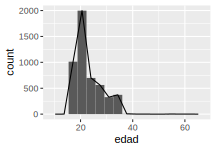
\includegraphics{EstadisticaParaCienciasSocialesConR_files/figure-latex/unnamed-chunk-146-1} \end{center}

La ojiva tiene una capa llamada \texttt{stat\_ecdf}, para el cálculo de la distribución de frecuencias acumuladas empíricas. Su sintaxis sigue la misma lógica: en \texttt{aes} se indica la variable que se grafica:

\begin{Shaded}
\begin{Highlighting}[]
\FunctionTok{ggplot}\NormalTok{(base.ejemplo) }\SpecialCharTok{+} \FunctionTok{stat\_ecdf}\NormalTok{(}\FunctionTok{aes}\NormalTok{(edad))}
\end{Highlighting}
\end{Shaded}

\begin{center}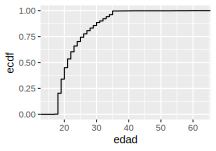
\includegraphics{EstadisticaParaCienciasSocialesConR_files/figure-latex/unnamed-chunk-147-1} \end{center}

Por defecto grafica escalones, que representan los saltos de frecuencia, se puede modificar por puntos, con el argumento \texttt{geom}:

\begin{Shaded}
\begin{Highlighting}[]
\FunctionTok{ggplot}\NormalTok{(base.ejemplo) }\SpecialCharTok{+} \FunctionTok{stat\_ecdf}\NormalTok{(}\FunctionTok{aes}\NormalTok{(edad), }\AttributeTok{geom =} \StringTok{"point"}\NormalTok{)}
\end{Highlighting}
\end{Shaded}

\begin{center}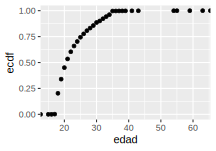
\includegraphics{EstadisticaParaCienciasSocialesConR_files/figure-latex/unnamed-chunk-148-1} \end{center}

O estilizando los escalones con una línea:

\begin{Shaded}
\begin{Highlighting}[]
\FunctionTok{ggplot}\NormalTok{(base.ejemplo) }\SpecialCharTok{+} \FunctionTok{stat\_ecdf}\NormalTok{(}\FunctionTok{aes}\NormalTok{(edad), }\AttributeTok{geom =} \StringTok{"line"}\NormalTok{)}
\end{Highlighting}
\end{Shaded}

\begin{center}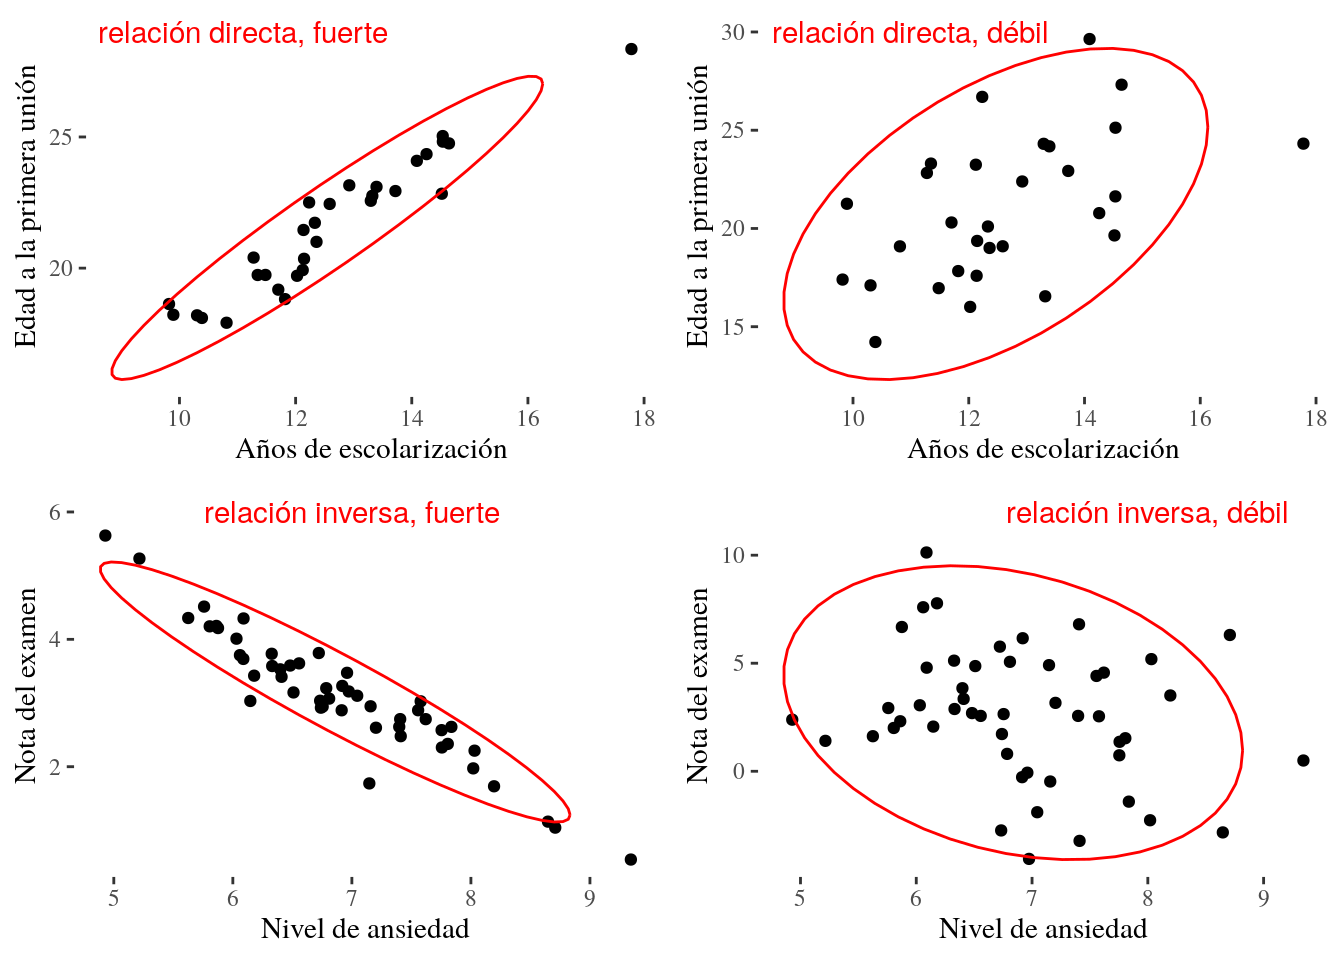
\includegraphics{EstadisticaParaCienciasSocialesConR_files/figure-latex/unnamed-chunk-149-1} \end{center}

Hay muchas opciones para mejorar la visualización de estos gráficos, que se irán presentando más adelante.

\chapter{La expresión resumida de la información}\label{la-expresiuxf3n-resumida-de-la-informaciuxf3n}

La segunda etapa en la descripción de datos consiste en calcular medidas que los resuman, que los expresen de manera sintética. Esta etapa implica un nuevo alejamiento de la información bruta, ya que se pierde de vista no solo a los individuos, que están presentes en la matriz de datos, sino también a las distribuciones de frecuencia. La ventaja de resumir es la posibilidad de presentar la información de modo muy sintético; con unas pocas medidas descriptivas se ofrece bastante información sobre los datos que se observan.

Estas medidas requieren operaciones de diferente nivel de complejidad, por lo que apelan a diferentes propiedades de las escalas de medición, entonces no serán las mismas las medidas que se puedan calcular en una escala nominal que en una ordinal, intervalar o proporcional.

El objetivo de describir el conjunto de datos se logrará indicando tres tipos diferentes de medidas. En primer lugar, haremos referencia a las medidas de \textbf{posición}. Estas medidas indican en torno a qué valores se distribuyen las observaciones. En segundo lugar, se describe la \textbf{forma} que toma la distribución, medida con dos indicadores: \textbf{simetría} y \textbf{curtosis}. En tercer lugar, se presentan las medidas de \textbf{dispersión} (conocidas también como de \textbf{variabilidad}), que muestran si los datos están concentrados alrededor de las medidas de centralidad o si están alejados de esas medidas centrales.

A los fines de la notación usada para referirse a cada una de estas
medidas descriptivas, asumiremos que trabajamos sobre datos provenientes de una muestra, de la que \emph{n} representa la cantidad de casos observados.

\section{Medidas de posición}\label{medidas-de-posiciuxf3n}

Como las operaciones que pueda hacerse entre las categorías dependen del nivel de medición de las variables, las medidas que se puedan calcular también dependerán de él. Por eso las presentaremos separadamente para cada nivel, siempre recordando que las operaciones que son válidas a un determinado nivel de medición también son válidas para niveles más altos. Por ejemplo: lo que pueda hacerse con variables nominales, vale también para ordinales y métricas, con los ajustes de casa caso.

\subsection{Variables nominales: proporciones}\label{variables-nominales-proporciones}

Cuando se trabaja con una variable de nivel nominal, una manera
sintética de presentar la información que ofrece la tabla de
distribución de frecuencias es indicando la \textbf{proporción} de casos que se encuentran en una determinada categoría. Se trata de la frecuencia relativa simple (\(f'\)) de una categoría particular. La siguiente es la distribución de las respuestas a la pregunta ``¿Con cuál de las siguientes frases está Ud. más de acuerdo?'' (P8STGBS), proveniente de la base latinobarómetro (2017, fraseo textual):

\begin{longtable}[]{@{}lcc@{}}
\toprule\noalign{}
¿Con qué frase está más de acuerdo? & f & f' \\
\midrule\noalign{}
\endhead
\bottomrule\noalign{}
\endlastfoot
Se puede confiar en la mayoría de las personas & 0.143 & 14.3 \\
Uno nunca es lo suficientemente cuidadoso en el trato con los demás & 0.857 & 85.7 \\
Total & 1 & 100 \\
\end{longtable}

Podemos indicar la proporción de personas que respondió que se puede confiar en la mayoría de las personas, como 0.143, que puede también expresarse como 14.3\%. La elección de cuál categoría se elige para indicar la proporción depende de los objetivos de la descripción. Al elegir una categoría se llama la atención sobre ella, se la destaca, ya que la proporción restante incluye a todas las demás categorías, las ``otras posibilidades''. Esa proporción restante se obtiene restando de 1 (uno) la proporción indicada, o restando de 100 (cien) si ha expresado como porcentaje. En este ejemplo, diremos que 0.857 (que proviene de hacer \$1- \$0.143) es la proporción de quienes no creen que se pueda confiar, o bien que estas personas representan el 85.7\% (85.7).

\begin{longtable}[]{@{}
  >{\centering\arraybackslash}p{(\linewidth - 0\tabcolsep) * \real{1.0000}}@{}}
\toprule\noalign{}
\endhead
\bottomrule\noalign{}
\endlastfoot
La \textbf{proporción} es la frecuencia relativa correspondiente a una categoría particular. Usualmente se expresa como porcentaje. Se indica como \(p\). \\
\end{longtable}

Esta medida descriptiva se usa a menudo cuando la variable nominal tiene solo dos categorías (variable dicotómica), ya que se presenta la proporción de una de ellas e inmediatamente se sabe que el complemento es la proporción de la otra.

Esta proporción puede también indicarse en variables de nivel de medición
superior al nominal, pero no resulta de interés cuando hay gran cantidad de categorías. Así, por ejemplo, si se trata de la distribución de las notas de un parcial, no resulta útil indicar cuál es la proporción de cada calificación e indicar algo como ``el 20\% sacó 8'' (lo que se vería en una tabla de distribución de frecuencias de las notas). Por el contrario, es común construir variables nominales a partir de las notas y, sí es de mucho interés indicar, por ejemplo, la proporción de quienes \emph{promocionaron}, o la proporción de quienes \emph{quedaron libres}, luego de haber categorizado las notas con un criterio teórico (el que define quiénes alcanzan las condiciones de promocional, regular y libre)

\subsection{Variables nominales: tasas}\label{variables-nominales-tasas}

Se define habitualmente como \textbf{tasa} a la frecuencia relativa de un
fenómeno en referencia a una población total, con la característica de tener en cuenta un período de tiempo. También es común el uso del
término cuando se trata de hechos de poca incidencia, es decir que su
frecuencia es pequeña. En esos casos se la suele expresar cada 1.000,
cada 10.000, o inclusive cada 100.000 casos, en lugar de por ciento. Por ejemplo, la tasa de desocupación en Argentina se define como la proporción de personas desocupadas, respecto del total de personas activas. Estas últimas son quienes tienen una ocupación o que sin tenerla la están buscando activamente. Está compuesta por la población ocupada más la población desocupada \citep{INDEC2011a}. Según INDEC, la tasa de desocupación en el segundo semestre de 2019 fue de 10.6\% (\url{https://www.indec.gob.ar/uploads/informesdeprensa/mercado_trabajo_eph_2trim19ED75D3E4D2.pdf}). Según la Organización Mundial de la Salud, en el año 2017, el cinco por mil de la población mundial vivía con VIH (\url{https://www.who.int/features/factfiles/hiv/es/})

Las tasas se usan especialmente para resumir procesos que suceden a lo largo del tiempo y se resumen en un momento dado. Esos procesos se captan mediante registros continuos, como los registros de nacimientos, defunciones, matrimoniales, de ingresos a hospitales, de declaración de residencia en municipios que lo solicitan. Por ejemplo, la tasa bruta de mortalidad se calcula dividiendo la cantidad de defunciones ocurridas en un período de tiempo (usualmente un año) y en un espacio geográfico (país, provincia, etc), por el total de la población que vivía en ese espacio geográfico a la mitad de ese año. La palabra ``bruta'' se refiere a que el cálculo de esta tasa no hace distinción por características de la población, como sexo o edad. Por el contrario, si se dividen las defunciones anuales de personas de una edad determinada por la cantidad de personas de esa edad que había a la mitad del año, se obtiene una tasa específica (por oposición a bruta) de mortalidad para esa edad.

\subsection{Variables nominales: razones}\label{variables-nominales-razones}

Las \textbf{razones} son cocientes calculados entre conjuntos que no tienen elementos en común. Por ejemplo, se llama razón de masculinidad a la cantidad de hombres por cada 100 mujeres que hay en una población. Se obtiene dividiendo el total de varones por el total de mujeres (y luego multiplicando por 100), que son dos conjuntos que no se superponen. Esta medida se conoce también como índice de masculinidad.

Según el censo de 2010, la siguiente es el distribución por sexos de la población de Argentina en ese momento:

\begin{longtable}[]{@{}lcc@{}}
\toprule\noalign{}
sexo & personas & prop.sexos \\
\midrule\noalign{}
\endhead
\bottomrule\noalign{}
\endlastfoot
varones & 19523766 & 0.487 \\
mujeres & 20593330 & 0.513 \\
Total & 40117096 & 1.000 \\
\end{longtable}

La proporción de varones es 48.7\% y la de mujeres de 51.3\%; se calculan respecto de la población total. La razón de feminidad se obtiene dividiendo el total de mujeres en el de varones y a la inversa para la de masculinidad. El cociente \(\frac{20593330}{19523766}*100\), que es 105.5 indica que hay en la población 105 mujeres por cada 100 varones.

Lo que distingue a las razones de las tasas y de las proporciones es que el numerador no está incluido en el denominador.

\subsection{Variables nominales: el modo}\label{variables-nominales-el-modo}

El \textbf{modo} o \textbf{moda} o \textbf{valor modal} es el valor de la variable
(la categoría) que tiene la mayor frecuencia. Dicho de otra manera, el valor de la variable más frecuentemente observado\footnote{Esta es la idea que transmite el lenguaje coloquial: cuando algo es ``la moda'', es lo que más comúnmente (frecuentemente) se ve.}. Esta medida no requiere ningún cálculo, no exige ninguna propiedad de la escala de
medición, por lo tanto se puede indicar en variables desde el nivel
nominal, es decir en todos los niveles de medición.

Por ejemplo, la variable \emph{carrera que cursa}, tiene la siguiente distribución:

\begin{longtable}[]{@{}lcc@{}}
\toprule\noalign{}
carrera & f & f' \\
\midrule\noalign{}
\endhead
\bottomrule\noalign{}
\endlastfoot
Educación & 44 & 0.29 \\
Psicología & 48 & 0.32 \\
Psicopedagogía & 58 & 0.39 \\
Total & 150 & 1.00 \\
\end{longtable}

El modo es Psicopedagogía, que es la categoría de mayor frecuencia. Debe cuidarse de no cometer el error de señalar la frecuencia 58 como el modo; el modo no es la frecuencia más alta, sino la categoría de la variable que tiene mayor frecuencia. Para hallarlo, se identifica la más alta de las frecuencias y se señala la categoría que le corresponde. Puede usarse la frecuencia absoluta o la relativa para determinar cuál es el modo de la distribución.

La pregunta ``¿Con cuál de las siguientes frases está Ud. más
de acuerdo?'' (P8STGBS), procedente de la base Latinobarómetro (2017), tiene la siguiente distribución de frecuencias:

\begin{verbatim}
##   [1] "X"          "numinves"   "idenpa"     "numentre"   "reg"       
##   [6] "ciudad"     "tamciud"    "comdist"    "codigo"     "diareal"   
##  [11] "mesreal"    "ini"        "fin"        "dura"       "totrevi"   
##  [16] "totcuot"    "totrech"    "totperd"    "numcasa"    "codsuper"  
##  [21] "supervvi"   "superven"   "codif"      "digit"      "wt"        
##  [26] "P1ST"       "P2ST"       "P3STGBS"    "P4STGBSC"   "P5STGBS"   
##  [31] "P6STICC1"   "P7STGBS"    "P8STGBS"    "P9STGBSC.A" "P9STGBS.B" 
##  [36] "P10ST"      "P11STGBSC"  "P12STC"     "P13STGBS"   "P14STGBS.A"
##  [41] "P14STGBS.B" "P14ST.C"    "P14ST.D"    "P14ST.E"    "P14ST.F"   
##  [46] "P14ST.G"    "P14ST.H"    "P15ST.A"    "P15ST.B"    "P15ST.C"   
##  [51] "P15ST.D"    "P15ST.E"    "P15ST.F"    "P15ST.G"    "P15ST.H"   
##  [56] "P15ST.I"    "P15ST.J"    "P15ST.K"    "P16STGBS"   "P16STGBS.A"
##  [61] "perpart"    "fampart"    "P17STGBSC"  "P18GBS"     "P19STC"    
##  [66] "P20ST"      "P21ST.A"    "P21ST.B"    "P21ST.C"    "P21ST.D"   
##  [71] "P21ST.E"    "P21ST.F"    "P21ST.G"    "P21ST.H"    "P22ST"     
##  [76] "P23STC"     "P24STC"     "P25STTI"    "P26ST"      "P27ST"     
##  [81] "P28N.A"     "P28N.B"     "P28N.C"     "P28N.D"     "P28N.E"    
##  [86] "P28N.F"     "P29NSPA"    "P29NSPB"    "P29NSPC"    "P29NSPD"   
##  [91] "P29NSPE"    "P29NSPF"    "P29NSPG"    "P29NSPH"    "P29NSPI"   
##  [96] "P29NSPJ"    "P29NSPZ"    "P29NSPX"    "P30NSP"     "P31NSP"    
## [101] "P32NSP.A"   "P33NSP"     "P34NA"      "P34NB"      "P35NC"     
## [106] "P36C"       "P37NC"      "P38ST"      "P39STTI"    "P40NC_A"   
## [111] "P40NC_B"    "P41STC.A"   "P41STC.B"   "P41STC.C"   "P42NC.A"   
## [116] "P42NC.B"    "P42NC.C"    "P42NC.D"    "P42NC.E"    "P42NC.F"   
## [121] "P43ST.A"    "P43ST.B"    "P44N"       "P45ST.A"    "P45N.B"    
## [126] "P45ST.C"    "P45ST.D"    "P45ST.E"    "P45N.F"     "P46ST.A"   
## [131] "P46ST.B"    "P46ST.C"    "P46ST.D"    "P46STM.E"   "P47N"      
## [136] "P48STM"     "P49STA.1"   "P49STA.2"   "P49STA.3"   "P49STA.4"  
## [141] "P49STA.5"   "P49STA.6"   "P49STA.7"   "P49STA.8"   "P49STB.1"  
## [146] "P49STB.2"   "P49STB.3"   "P49STB.4"   "P49STB.5"   "P49STB.6"  
## [151] "P49STB.7"   "P49STB.8"   "P50STM"     "P51STMA"    "P51STMB"   
## [156] "P51STMC"    "P51STMD"    "P51STME"    "P51STMF"    "P51STMG"   
## [161] "P51STMH"    "P51STMI"    "P51STMJ"    "P51STMK"    "P51STMZ"   
## [166] "P52NA"      "P52NB"      "P52NC"      "P52ND"      "P52NE"     
## [171] "P52NF"      "P52NZ"      "P53ST.A"    "P53N.B"     "P53N.C"    
## [176] "P53N.D"     "P53N.E"     "P53N.F"     "P53N.G"     "P53N.H"    
## [181] "P53N.I"     "P54STMA"    "P54STMB"    "P54STMC"    "P54STMD"   
## [186] "P54STME"    "P54STMF"    "P54STMG"    "P54STMH"    "P54STMI"   
## [191] "P54STMJ"    "P54STMX"    "P54STMZ"    "P55N.A"     "P55N.B"    
## [196] "P55N.C"     "P56N.A"     "P56N.B"     "P56N.C"     "P56N.D"    
## [201] "P56N.E"     "P56N.F"     "P56N.G"     "P57N"       "P58N"      
## [206] "P59N"       "P60N"       "P61ST.1"    "P61ST.2"    "P61ST.3"   
## [211] "P62NA"      "P62NB"      "P62NC"      "P62ND"      "P62NE"     
## [216] "P62NF"      "P62NG"      "P62NH"      "P62NI"      "P62NJ"     
## [221] "P62NK"      "P62NX"      "P62NY"      "P62NZ"      "P63A"      
## [226] "P63B"       "P63C"       "P63D"       "P63E"       "P63F"      
## [231] "P63G"       "P63H"       "P63I"       "P63J"       "P63K"      
## [236] "P63X"       "P63Y"       "P63Z"       "P64STAA"    "P64STAB"   
## [241] "P64STAC"    "P64STAD"    "P64STAE"    "P64STAF"    "P64STAG"   
## [246] "P64STAH"    "P64STAZ"    "P64STBA"    "P64STBB"    "P64STBC"   
## [251] "P64STBD"    "P64STBE"    "P64STBF"    "P64STBG"    "P64STBH"   
## [256] "P64STBZ"    "P65ST.A"    "P65ST.B"    "P66ST"      "P67NBCS"   
## [261] "P68NBCS"    "P69NBCS"    "P70N_A"     "P70N_B"     "P71N"      
## [266] "P72NR"      "P73NR"      "P74NR"      "P75NR"      "P76NR"     
## [271] "sexo"       "S1"         "edad"       "S2"         "S3"        
## [276] "S4"         "S5"         "S6"         "S7"         "S8"        
## [281] "S9"         "S9.A"       "S10"        "S11"        "S12"       
## [286] "S13"        "S14"        "REEDUC.1"   "S15"        "REEDUC.2"  
## [291] "reedad"     "S16M_A"     "S16M_B"     "S16M_C"     "S16M_D"    
## [296] "S16M_E"     "S16M_F"     "S16M_G"     "S16M_H"     "S16M_I"    
## [301] "S16M_K"     "S16M_J"     "S17.A"      "S17.B"      "S17.C"     
## [306] "S17.E"      "S17.F"      "S17.G"      "S17.I"      "S17.J"     
## [311] "S17.K"      "S17.L"      "S17.M"      "S17.N"      "S18.A"     
## [316] "S18.B"      "S19"        "S20"        "S20.A"      "S20.B"     
## [321] "S21"        "S22"        "S23"        "S24.A"      "S24.B"
\end{verbatim}

\begin{verbatim}
## 
##    -2    -1     1     2     3 
##   243  1571 10785  2526  5075
\end{verbatim}

\begin{longtable}[]{@{}lc@{}}
\toprule\noalign{}
P8STGBS & f \\
\midrule\noalign{}
\endhead
\bottomrule\noalign{}
\endlastfoot
La democracia es preferible a cualquier otra forma de gobierno & 10785 \\
En algunas circunstancias, un gobierno autoritario puede ser preferible a uno democrático & 2526 \\
A la gente como uno, nos da lo mismo un régimen democrático que uno no democrático & 5075 \\
\end{longtable}

Allí, la categoría modal es la que privilegia a la democracia como sistema de gobierno.

Si se trata de una variable de mayor nivel de medición, no hay ninguna diferencia. La variable \emph{concepto asignado a estudiantes por parte de sus docentes}, que es de nivel ordinal, tiene la distribución de frecuencias siguiente:

\begin{longtable}[]{@{}lc@{}}
\toprule\noalign{}
concepto & f \\
\midrule\noalign{}
\endhead
\bottomrule\noalign{}
\endlastfoot
Excelente & 150 \\
Muy bueno & 350 \\
Bueno & 200 \\
Satisfactorio & 120 \\
No satisfactorio & 50 \\
Total & 870 \\
\end{longtable}

En este ejemplo, 350 es la frecuencia más alta, por lo tanto, la
categoría que a ella corresponde es el modo: el modo de la distribución es ``Muy bueno''.

\begin{longtable}[]{@{}
  >{\centering\arraybackslash}p{(\linewidth - 0\tabcolsep) * \real{1.0000}}@{}}
\toprule\noalign{}
\endhead
\bottomrule\noalign{}
\endlastfoot
El \textbf{modo} es la categoría ──o el valor── de la variable que tiene mayor frecuencia. Se indica \(M_o\). \\
\end{longtable}

Cuando se trabaja sobre variables intervalares o proporcionales
discretas no hay diferencia en la identificación del modo de la
distribución. El \emph{número de materias que tienen aprobadas quienes han terminado de cursar el primer año} de su carrera se distribuye así:

\begin{longtable}[]{@{}lc@{}}
\toprule\noalign{}
Cantidad de materias aprobadas & f \\
\midrule\noalign{}
\endhead
\bottomrule\noalign{}
\endlastfoot
0 & 30 \\
1 & 150 \\
2 & 200 \\
3 & 300 \\
4 & 250 \\
5 & 200 \\
6 & 20 \\
Total & 1150 \\
\end{longtable}

En esta distribución, el modo es 3 materias aprobadas (\(M_o = 3\)), que es la categoría que tiene mayor frecuencia. Expresamos esto como ``la mayor cantidad de quienes terminaron de cursar primer año han aprobado tres materias''.

Puede suceder que en una distribución no haya una única categoría de
mayor frecuencia, sino que dos o más compartan la mayor frecuencia. Para 160 estudiantes según la facultad en que cursan su carrera, tenemos:

\begin{longtable}[]{@{}lc@{}}
\toprule\noalign{}
Facultad a la que pertenece & f \\
\midrule\noalign{}
\endhead
\bottomrule\noalign{}
\endlastfoot
Arquitectura & 50 \\
Ingeniería & 40 \\
Psicología & 50 \\
Sociales & 20 \\
Total & 160 \\
\end{longtable}

Vemos aquí que hay dos categorías que presentan la mayor frecuencia:
Arquitectura y Psicología. Decimos en este caso que la distribución es \textbf{bimodal} que quiere decir que tiene dos modos.

\begin{longtable}[]{@{}
  >{\centering\arraybackslash}p{(\linewidth - 0\tabcolsep) * \real{1.0000}}@{}}
\toprule\noalign{}
\endhead
\bottomrule\noalign{}
\endlastfoot
Una distribución es \textbf{bimodal} cuando dos categorías tienen la mayor frecuencia. Si son más las categorías que comparten la mayor frecuencia, la distribución se denomina \textbf{multimodal}. \\
\end{longtable}

Una representación gráfica de una distribución bimodal, para la variable \emph{número de respuestas correctas en una prueba de opción múltiple}, la siguiente:

\begin{figure}[H]

{\centering 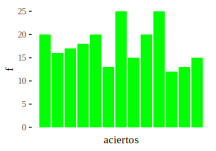
\includegraphics{EstadisticaParaCienciasSocialesConR_files/figure-latex/unnamed-chunk-158-1} 

}

\caption{Distribución del  número de aciertos}\label{fig:unnamed-chunk-158}
\end{figure}

Con modo en 6 y 9 aciertos, por eso se llama bimodal.

La moda tiene el inconveniente de ser independiente de la mayor parte de los datos, por lo que no es sensible a cambios en los valores de la
distribución. En efecto, las siguientes dos muestras de 130 escuelas
tienen la misma moda (\(M_o = Pública\)), aunque son muy diferentes:

\begin{longtable}[]{@{}lclc@{}}
\toprule\noalign{}
Gestión de la escuela & f & Gestión de la escuela & f \\
\midrule\noalign{}
\endhead
\bottomrule\noalign{}
\endlastfoot
Pública & 50 & Pública & 100 \\
Privada laica & 45 & Privada laica & 20 \\
Privada confesional & 35 & Privada confesional & 10 \\
Total & 130 & Total & 130 \\
\end{longtable}

\subsection{Variables ordinales: cuantiles}\label{variables-ordinales-cuantiles}

Como ya hemos visto, cuando las categorías de la variable están
ordenadas pueden hacerse juicios como ``mayor que'' (\(>\)) o ``menor que''
(\(<\)), y el nivel de medición es ordinal. En este tipo de variables
puede calcularse un conjunto de medidas de posición, que usan esa propiedad: la del orden entre categorías. Se trata de los \textbf{cuantiles}, que se podrán también calcular para escalas superiores (intervalar y proporcional) pero no para escalas nominales, en las que el orden entre categorías no está presente.
Los cuantiles usan las frecuencias relativas acumuladas, por eso solo existen para variables de nivel superior al nominal. Veamos la presentación por medio de un ejemplo, con la tabla siguiente que tiene calculadas las frecuencias relativas acumuladas de las edades de estudiantes de una carrera universitaria, y se muestran solo ellas:

\begin{longtable}[]{@{}cc@{}}
\toprule\noalign{}
edad & F' \\
\midrule\noalign{}
\endhead
\bottomrule\noalign{}
\endlastfoot
17 & 0.00 \\
18 & 0.07 \\
19 & 0.16 \\
20 & 0.26 \\
21 & 0.36 \\
22 & 0.46 \\
23 & 0.55 \\
24 & 0.61 \\
25 & 0.68 \\
26 & 0.73 \\
27 & 0.77 \\
28 & 0.80 \\
29 & 0.83 \\
30 & 0.85 \\
31 & 0.87 \\
32 & 0.89 \\
33 & 0.91 \\
34 & 0.92 \\
35 & 0.93 \\
36 & 0.94 \\
37 & 0.95 \\
38 & 0.95 \\
39 & 0.96 \\
40 & 0.96 \\
41 & 0.97 \\
42 & 0.97 \\
43 & 0.98 \\
44 & 0.98 \\
45 & 0.98 \\
46 & 0.99 \\
47 & 0.99 \\
48 & 0.99 \\
49 & 0.99 \\
50 & 0.99 \\
51 & 1.00 \\
52 & 1.00 \\
53 & 1.00 \\
54 & 1.00 \\
\end{longtable}

La frecuencia acumulada 0.26 es la proporción de estudiantes que tiene 20 años o menos. Se dice que el valor 20 años es el cuantil 0.26. El ``cuantil'' en sí mismo no es una medida descriptiva, para que lo sea se debe especificar \emph{qué} cuantil es el que se calcula. En este ejemplo, cada frecuencia acumulada conduce a un cuantil particular. El cuantil 0.68 de la variable es 25 años. Estas medidas se definen como el valor de la variable que deja por debajo una determinada proporción de observaciones.
Es muy frecuente expresar los cuantiles en términos de porcentaje, para facilitar la comunicación, y se los llama percentiles. De este modo, el cuantil 0.26 equivale a decir percentil 26, que se escribe \(P_{26}\) y el cuantil 0.68 se escribe \(P_{68}\). Así, escribimos para la tabla de arriba: \[P_{26}=20\] y \[P_{68}=25\].

\begin{longtable}[]{@{}
  >{\centering\arraybackslash}p{(\linewidth - 0\tabcolsep) * \real{1.0000}}@{}}
\toprule\noalign{}
\endhead
\bottomrule\noalign{}
\endlastfoot
Se denominan \textbf{cuantiles} los valores de la variable que dejan por debajo una determinada proporción de las observaciones. El cuantil \(r\) (con \(0<r<1\)) deja por debajo una proporción \(r\) de casos, y una proporción \(1-r\) de los casos está por encima de él. Cuando las proporciones se expresan como porcentajes, se los denomina \textbf{percentiles} \\
\end{longtable}

Los cuantiles tienen utilidad como medidas resumen cuando hay un volumen importante de observaciones, de lo contrario, es preferible mostrar la serie de datos. Su aplicación es que permiten describir cada valor de la variable de manera relativa al conjunto completo. Si alguien obtuvo una nota que corresponde al percentil 95 (cuantil 0.95), se sabe que es una nota alta, porque el 95\% del conjunto de quienes participaron de la prueba tiene una nota como esa o inferior, o bien que solo el 5\% del conjunto tiene nota superior a la de él.

A continuación veremos algunos medidas que se definen del mismo modo que los cuantiles; en base a las frecuencias relativas acumuladas.

\subsubsection{La mediana}\label{la-mediana}

La \textbf{mediana} es el cuantil \(0.50\) o bien el percentil \(50\). Se define como el valor que \emph{supera a} y \emph{es superado por} no más de la mitad de las observaciones. Es el valor que deja por debajo de sí y por encima de sí \emph{a lo sumo} la mitad de las observaciones. Es importante tener en cuenta que se trata de la mitad de los casos y no la mitad de las categorías. La siguiente distribución presenta en serie simple ordenada el número de sesiones de psicoterapia que recibieron 9 pacientes en un hospital:

\[2,\: 2,\: 3,\: 5,\: 7,\: 10, \:15, \:19, \:50\]

La mediana de estos datos es 7, porque es el valor que deja cuatro casos por debajo y también cuatro casos por encima, que es menos de la mitad de los 9 casos. La serie simple tiene que estar ordenada para poder identificar a la mediana.

Si la cantidad de observaciones fuera par como por ejemplo:

\[2, \:2,\: 3,\: 5,\: 7,\: 10,\: 15, \:19\]

El punto de corte correspondiente a la mitad de las observaciones se
ubica entre 5 y 7, en este caso, por convención, la mediana se considera el promedio entre los dos valores centrales, que es 6. Y la mediana deja exactamente a la mitad de los casos por encima y por debajo de ella.

Cuando hay valores repetidos en la parte central, ningún valor deja exactamente la mitad por encima y por debajo. Por ejemplo si la serie fuera:

\[2,\: 3,\: 7,\: 7,\: 7,\: 10,\: 15,\: 19\]

El valor 7 es la mediana, porque es \emph{superado} por tres
valores (10, 15 y 19), que es menos de la mitad; y \emph{supera} a dos (2 y 3), que es menos de la mitad.

La mediana es una medida muy adecuada cuando se necesitan resumir datos que provienen de escalas ordinales o de nivel superior. Sin embargo, su cálculo no aporta nada en series simples con pocos casos (como los que acabamos de ver) ya que allí es más sencillo mostrar el conjunto completo de datos y no usar medidas resumen. Los ejemplos anteriores sirven para ilustrar el concepto, pero no se usa así en la práctica. Las operaciones de resumen se justifican cuando se tiene un conjunto grande de datos.

\begin{longtable}[]{@{}
  >{\centering\arraybackslash}p{(\linewidth - 0\tabcolsep) * \real{1.0000}}@{}}
\toprule\noalign{}
\endhead
\bottomrule\noalign{}
\endlastfoot
Se denomina \textbf{mediana} al valor de la variable que deja por debajo a la mitad o más de las observaciones y que deja por encima a la mitad o más de las observaciones. Corresponde al cuantil 0.50. Si la variable es continua, la mediana deja la misma cantidad de casos por debajo y por encima de ella. Si la variable es discreta deja por debajo la mitad o más de los casos, y deja encima la mitad o más de los casos. Se indica \(M_{dn}\). \\
\end{longtable}

Veamos la forma de reconocer a la mediana cuando los datos están
presentados en una distribución de frecuencias. La siguiente es una
clasificación de hogares por nivel socioeconómico:

\begin{longtable}[]{@{}lccl@{}}
\toprule\noalign{}
Nivel socioeconómico & f (número de hogares) & F & F´ \\
\midrule\noalign{}
\endhead
\bottomrule\noalign{}
\endlastfoot
Marginal & 40 & 40 & 0.09 \\
Bajo & 100 & 140 & 0.32 \\
Medio-bajo & 120 & 260 & 0.59 \\
Medio & 150 & 410 & 0.93 \\
Alto & 30 & 440 & 1.00 \\
Total & 440 & & \\
\end{longtable}

El valor de la variable que acumula el 50\% de los casos, es el que ocupa el lugar 220, que es mitad de los 440 casos del total. La serie ordenada de esta distribución, coloca a los 40 hogares de nivel socioeconómico ``marginal'' en los primeros 40 lugares, pero indistintamente, porque no hay orden entre los hogares al interior de la categoría. Según la tabla, hasta la categoría ``medio-bajo'' se acumulan 260 hogares y hasta la categoría anterior hay 140 acumulados. De manera que el hogar que ocupa el lugar 220 (de la serie ordenada) es uno de los que se encuentran en la categoría ``medio-bajo''. Diremos así que la mediana de esta distribución es ``medio-bajo''. Como puede verse, esta categoría no acumula exactamente la mitad de las observaciones, pero es la que contiene a la observación que supera a la mitad y es superada por la otra mitad. Por esa razón la leemos como la mediana, diciendo que la mitad de los hogares tiene un nivel socioeconómico medio-bajo o inferior a ese. Decir que el que acumula 220 casos es ``uno de los hogares de la categoría medio-bajo'' se fundamenta en que todos los hogares son equivalentes en su nivel socioeconómico al interior de la categoría.

La misma interpretación corresponde si se trata de
una variable cuantitativa discreta. Si la variable es el \emph{número de síntomas} a partir de los cuales fue diagnosticado de esquizofrenia un conjunto de pacientes\footnote{El manual DSM IV indica como síntomas característicos a dos (o más) de los siguientes, cada uno de ellos presente durante una parte significativa de un período de 1 mes: ideas delirantes, alucinaciones, lenguaje desorganizado (p.~ej., descarrilamiento frecuente o incoherencia), comportamiento catatónico o gravemente desorganizado, síntomas negativos, por ejemplo, aplanamiento afectivo, alogia o abulia.}:

\begin{longtable}[]{@{}lcc@{}}
\toprule\noalign{}
Cantidad de síntomas & f (número de pacientes) & F \\
\midrule\noalign{}
\endhead
\bottomrule\noalign{}
\endlastfoot
2 & 30 & 30 \\
3 & 60 & 90 \\
4 & 70 & 160 \\
5 & 90 & 250 \\
Total & 250 & \\
\end{longtable}

La mitad del número total de casos es de 125 (\(250/2\) ó \((1/2)*250\)), ¿cuál
es el caso que ocupa ese lugar? Vemos que hasta 3 síntomas se acumulan
90 pacientes y 160 hasta los 4. Quien ocupa el puesto 125 en
la serie simple ordenada está entre quienes recibieron su diagnóstico a
partir de 4 síntomas. Por esa razón indicamos a la mediana con ese
valor: 4, \(M_{dn} = 4\) que es el que cumple con la definición de superar a y ser superado por, no más de la mitad de las observaciones. Así, la primera categoría que tenga una frecuencia acumulada superior al 50\% será la que contenga a la mediana. Es así porque, tanto las categorías anteriores a 4 como las posteriores reúnen menos de la mitad de las observaciones. La lectura del resultado es que la mitad de
los diagnósticos de esquizofrenia se realizó a partir de la presencia de cuatro síntomas o menos.

Sea la variable \emph{número de materias aprobadas por estudiantes de segundo año de una carrera universitaria}:

\begin{longtable}[]{@{}lcc@{}}
\toprule\noalign{}
Número de materias aprobadas & f & F \\
\midrule\noalign{}
\endhead
\bottomrule\noalign{}
\endlastfoot
0 & 30 & 30 \\
1 & 150 & 180 \\
2 & 200 & 380 \\
3 & 300 & 680 \\
4 & 250 & 930 \\
5 & 200 & 1130 \\
6 & 20 & 1150 \\
Total & 1150 & \\
\end{longtable}

La mitad de 1150 es 575, la primera frecuencia acumulada que supera a
575 es 680, que corresponde al valor 3. La mediana de esta distribución es entonces tres materias aprobadas y diremos que el 50\% de este grupo de estudiantes aprobó tres materias o menos.

Cuando se trata de variables de nivel intervalar o proporcional y con
categorías agrupadas, el cálculo anterior puede refinarse. Así, primero se identifica la categoría (el intervalo) en que se encuentra la mediana, igual que en los dos ejemplos anteriores y luego se interpola dentro del intervalo para encontrar su valor exacto.\\
Sea la variable \emph{tiempo de reacción a un estímulo visual expresado en segundos} medido en un experimento que tuvo 34 participantes.

\begin{longtable}[]{@{}lcc@{}}
\toprule\noalign{}
Tiempo de reacción (en segundos) & f & F \\
\midrule\noalign{}
\endhead
\bottomrule\noalign{}
\endlastfoot
1.0 - 1.5 & 5 & 5 \\
1.5 - 2.0 & 7 & 12 \\
2.0 - 2.5 & 6 & 18 \\
2.5 - 3.0 & 3 & 21 \\
3.0 - 3.5 & 8 & 29 \\
3.5 - 4.0 & 5 & 34 \\
Total & 34 & \\
\end{longtable}

La mitad de las 34 observaciones es 17, por lo que debe encontrarse una
observación que tenga frecuencia acumulada de 17. Ese valor no aparece
en la F, el primero que lo supera es 18, entonces la mediana estará en
el intervalo \(2.0\:-\:2.5\). Esto es así porque hasta 2.0 se acumulan 12 casos
(la F de la categoría anterior) y hasta 2.5 se acumulan 18. Nuestros 17
casos se acumulan para un valor de la variable que está entre 2.0 y 2.5.

Debemos ahora encontrar qué valor exactamente es la mediana, dentro del
intervalo 2.0-2.5. La fórmula para este procedimiento es la siguiente:

\[M_{dn} = l_{i} + i*\left( \frac{\frac{n}{2} - F_d}{f_{p}} \right)\]

En la que:

\begin{itemize}
\item
  \(l_i\) indica el límite inferior del intervalo en que se encuentra la mediana, en este caso es 2.0.
\item
  \(i\) es la amplitud del intervalo, es decir la diferencia entre los límites \(2.0-2.5 = 0.5\).
\item
  \(\frac{n}{2}\) es la mitad del número total de observaciones, es este caso, 17.
\item
  \(F_d\) es la frecuencia acumulada por \textbf{d}ebajo de la categoría que contiene la mediana, en esta tabla es 12.
\item
  \(f_p\) es la frecuencia \textbf{p}ropia del intervalo en que se encuentra la mediana. Es la frecuencia absoluta (no la acumulada), en este ejemplo es 6.
\end{itemize}

Reemplazando resulta:

\[M_{dn} = 2.0 + 0.5*\left( \frac{17 - 12}{6} \right) = 2.0 + 0.5*\left( \frac{5}{6} \right) = 2.42\]

Conviene detenerse en el orden en que se realizaron las operaciones. El
signo más (+) separa términos, por lo que primero debe resolverse el
segundo de ellos y luego recién sumar 2.0. Un error frecuente es el de
sumar \(2.0 + 0.5\) y luego multiplicar por el resultado del paréntesis, eso
es incorrecto.

Por cierto que debe verificarse que el valor encontrado se ubique dentro
del intervalo; en este ejemplo, la mediana no podría ser menor que 2.0
ni mayor que 2.5. Observemos también que el número de categorías de la
variable, que es de 6, no participa en el cálculo de la mediana, de
ningún modo se trata de una categoría que esté ``al medio''.

El resultado obtenido nos dice, según la definición de la mediana que
``el 50\% de quienes participaron del experimento reaccionó en un tiempo de 2.42 segundos o inferior''. Es muy importante la última parte de la lectura,
porque cuando decimos ``o inferior'' incluimos los valores por debajo del indicado. De lo contrario, si se omite ``o menos'' se estaría diciendo que la mitad del grupo coincidió \emph{exactamente} en 2.42 segundos.

La mediana encontrada, de 2.42, es un valor razonable a partir de la
observación de la tabla: la categoría de la mediana acumulaba 18 casos,
que es apenas más que la mitad de las observaciones (17), por lo que era
de esperar que la mediana apareciera cerca del límite superior del
intervalo, que es lo que sucedió.

Este procedimiento para calcular la mediana es imperfecto, porque supone que los valores están distribuidos de manera uniforme dentro de cada intervalo. Si los 6 valores que contiene el intervalo 2.0 -- 2.5, fueran
todos iguales a 2.01, por ejemplo, la mediana sería un número bastante
menor al que se calculó con este método. El uso de la interpolación solo
se justifica en situaciones en que la única información disponible es la
tabla con los valores agrupados; por el contrario, si se cuenta con la
matriz de datos, el cálculo debe hacerse usando todos los valores
observados de la variable. Como esto es largo para hacer manualmente, se
solicita a un software especializado.

\subsubsection{Los cuartiles}\label{los-cuartiles}

Cuando la variable tiene un nivel de medición ordinal o superior, se puede usar el mismo razonamiento con el que definimos la mediana para
hacer cortes más finos en una distribución de frecuencia. Así, si la
mediana nos indica el valor de la variable que deja por debajo la mitad
de los casos, es lícito preguntar también por el valor que deja por
debajo un cuarto de los casos, o también el que deja por debajo las tres
cuartas partes de las observaciones. Estos puntos de corte se denominan
respectivamente: \textbf{primer cuartil} y \textbf{tercer cuartil}.

\begin{longtable}[]{@{}
  >{\centering\arraybackslash}p{(\linewidth - 0\tabcolsep) * \real{1.0000}}@{}}
\toprule\noalign{}
\endhead
\bottomrule\noalign{}
\endlastfoot
El \textbf{primer cuartil} es el valor de la variable que deja por debajo un \\
cuarto, o el 25\% del total de observaciones. Corresponde al cuantil 0.25 \\
\end{longtable}

\begin{longtable}[]{@{}
  >{\centering\arraybackslash}p{(\linewidth - 0\tabcolsep) * \real{1.0000}}@{}}
\toprule\noalign{}
\endhead
\bottomrule\noalign{}
\endlastfoot
El \textbf{tercer cuartil} es el valor que deja por debajo las tres cuartas \\
partes o el 75\% del total de observaciones. Corresponde al cuantil 0.75 \\
\end{longtable}

Como se ve, tanto el modo de cálculo como la interpretación son análogos a la mediana. Veamos su aplicación a los ejemplos anteriores:

\begin{longtable}[]{@{}lcc@{}}
\toprule\noalign{}
Número de materias aprobadas & f & F \\
\midrule\noalign{}
\endhead
\bottomrule\noalign{}
\endlastfoot
0 & 30 & 30 \\
1 & 150 & 180 \\
2 & 200 & 380 \\
3 & 300 & 680 \\
4 & 250 & 930 \\
5 & 200 & 1130 \\
6 & 20 & 1150 \\
Total & 1150 & \\
\end{longtable}

Para encontrar el primer cuartil será ahora necesario buscar un cuarto
del total de casos: 287.5 (\(\frac{1}{4}*1150\)). La pregunta ahora es ¿cuál es
la primera frecuencia acumulada que supera a 287.5? se trata de 380, que
corresponde al valor 2 y éste es entonces el primer cuartil. Leemos así
que un cuarto del total tiene dos materias aprobadas o menos.
También puede decirse que el 25\% del grupo aprobó dos materias o
menos. Si se toma la cantidad de materias aprobadas como un indicador
del ritmo más rápido o más lento de avance en la carrera, aquí se lee
que el 25\% que avanza con más lentitud no llegó a aprobar tres materias.

\begin{longtable}[]{@{}
  >{\centering\arraybackslash}p{(\linewidth - 0\tabcolsep) * \real{1.0000}}@{}}
\toprule\noalign{}
\endhead
\bottomrule\noalign{}
\endlastfoot
El \textbf{primer cuartil} es el valor de la variable que deja un cuarto (25\%) de los casos por debajo y tres cuartos (75\%) por encima. Se indica \(Q_1\). \\
\end{longtable}

Idéntico razonamiento seguimos para calcular el tercer cuartil: las tres
cuartas partes del total es 862.5 (\(\frac{3}{4}*1150\)). Buscamos luego la
primera frecuencia acumulada que supera a ese valor y hallamos que es
930 y que su categoría correspondiente es 4. Entonces el tercer cuartil
es 4 materias aprobadas. La lectura será: las tres cuartas partes (o el
75\%) de quienes cursan segundo año de la carrera lleva aprobadas cuatro materias o menos. Esto último implica
que el 25\% restante aprobó más de cuatro materias. Así, el grupo que
avanza más rápido en la carrera aprobó más de cuatro materias en su
primer año.

\begin{longtable}[]{@{}
  >{\centering\arraybackslash}p{(\linewidth - 0\tabcolsep) * \real{1.0000}}@{}}
\toprule\noalign{}
\endhead
\bottomrule\noalign{}
\endlastfoot
El \textbf{tercer cuartil} es el valor de la variable que deja tres cuartos (75\%) de los casos por debajo y un cuarto (25\%) por encima. Se indica \(Q_3\). \\
\end{longtable}

Cuando se trata de distribuciones con categorías agrupadas, procedemos
como antes con una leve modificación en la fórmula:

\begin{longtable}[]{@{}lcc@{}}
\toprule\noalign{}
Tiempo de reacción (en segundos) & f & F \\
\midrule\noalign{}
\endhead
\bottomrule\noalign{}
\endlastfoot
1.0 - 1.5 & 5 & 5 \\
1.5 - 2.0 & 7 & 12 \\
2.0 - 2.5 & 6 & 18 \\
2.5 - 3.0 & 3 & 21 \\
3.0 - 3.5 & 8 & 29 \\
3.5 - 4.0 & 5 & 34 \\
Total & 34 & \\
\end{longtable}

Para el primer cuartil debe hallarse la primera frecuencia que supera a
un cuarto de las observaciones, de las 34, un cuarto es 8.5 y la primera
frecuencia mayor que ese número es 12, por lo que el primer cuartil se
encuentra en la categoría \(1.5\:-\:2.0\). Para interpolar en valor exacto
usamos una expresión equivalente a la de la mediana:

\[Q_{1} = l_{i} + i*\left( \frac{\frac{n}{4} - f_{d}}{f_{p}} \right)\]

En la que se cambia \(\frac{n}{2}\) por \(\frac{n}{4}\) y lo demás mantiene
el mismo significado. Aplicándola a estos datos resulta:

\[Q_{1} = 1.5 + 0.5*\left( \frac{8.5 - 5}{7} \right) = 1.5 + 0.5*\left( 0.5 \right) = 1.75\]

Leemos en resultado como: el 25\% de quienes participaron del experimento reaccionó en un tiempo de 1.75 segundos o menos.

Para el tercer cuartil la fórmula se transforma en:

\[Q_{3} = l_{i} + i*\left( \frac{\frac{3*n}{4} - f_{d}}{f_{p}} \right)\]

Cuyo cambio consiste en que va \(\frac{3*n}{4}\) en lugar de \(\frac{n}{4}\)
y manteniendo el resto de los símbolos con el mismo significado.

Usando esta expresión, verifique que para la distribución de los tiempos de reacción, el tercer cuartil es 3.28.

No hemos hecho mención a un ``segundo cuartil'', que sería el valor de la
variable que acumula las dos cuartas partes de los casos, pero como las
dos cuartas partes es la mitad, se trata simplemente de la mediana
\(Q_{2} = M_{dn}\), el cuantil 0.50.

\subsubsection{Los percentiles}\label{los-percentiles}

Por el mismo camino pueden definirse cortes en otros puntos de la
distribución, los más frecuentemente usados, por su generalidad, se
conocen como \textbf{percentiles}. Se trata de valores de la variable que dejan
por debajo (acumulan) distintos porcentajes de casos.

\begin{longtable}[]{@{}
  >{\centering\arraybackslash}p{(\linewidth - 0\tabcolsep) * \real{1.0000}}@{}}
\toprule\noalign{}
\endhead
\bottomrule\noalign{}
\endlastfoot
El \textbf{percentil \(r\)} de una distribución es el valor de la variable que deja el \(r\) por ciento de los casos por debajo de él y \((100-r)\) por ciento de los casos por encima. Se indica \(P_r\). \\
\end{longtable}

Así por ejemplo, el percentil 10 (indicado como \(P_{10}\)) es el valor de
la variable que acumula el 10\% de las observaciones. Se representa de
modo general un percentil dado como \(P_r\) en el que \(r\) indica el
porcentaje del que se trata. La expresión para el cálculo de cualquier
percentil es:

\[P_{r} = l_{i} + i*\left( \frac{\frac{r}{100}*n - f_{d}}{f_{p}} \right)\]

Son fáciles de observar las siguientes equivalencias:

\[Q_{1} = P_{25}\]
\[M_{dn} = P_{50}\]
\[Q_{3} = P_{75}\]

También suelen mencionarse, en algunas publicaciones, otros puntos de
corte, como por ejemplo los \textbf{quintiles}, muy comunes para establecer cortes en los niveles de ingreso y corresponden a los cuantiles 0.20, 0.40, 0.60 y 0.80. Esta medida representa valores que acumulan quintos (20\%) de la distribución. La equivalencia es la siguiente:

\begin{longtable}[]{@{}lc@{}}
\toprule\noalign{}
Quintil: & Equivale a: \\
\midrule\noalign{}
\endhead
\bottomrule\noalign{}
\endlastfoot
Primero & \(P_{20}\) \\
Segundo & \(P_{40}\) \\
Tercero & \(P_{60}\) \\
Cuarto & \(P_{80}\) \\
\end{longtable}

El primer quintil de ingresos representa el valor de ingreso que deja por debajo al 20\% que tiene los menores ingresos. Por ejemplo según la EPH del tercer trimestre de 2018, el primer quintil de ingresos salariales era de 7000 pesos; la lectura es que el 20\% de personas asalariadas con los menores ingresos, los tenía por debajo de 7000 pesos.
Para los cálculos con la fórmula de interpolación se reemplaza el
\(\frac{n}{2}\) de la mediana por \(\frac{r}{100}\) para el percentil \(r\).
Esta manera de calcular los percentiles tiene la misma limitación
mencionada para la mediana.

Los cortes que generan 10 grupos con la misma cantidad de casos se llaman \textbf{deciles} (cuantiles desde 0.10 hasta 0.90). Por ejemplo, el segundo decil se escribe \(D_2\) es el valor de la variable que deja por debajo al 20\% de los casos, por lo que coincide con el primer quintil, el percentil 20 y el cuantil 0.20.

Así, la mediana, los cuartiles, quintiles, deciles y percentiles son todos cuantiles particulares. La mediana es el cuantil 0.50, define dos grupos con la mitad de los casos en cada uno; los cuartiles definen cuatro (con 25\% en cada uno), los quintiles cinco (con 20\% en cada uno), los deciles diez. Los percentiles cortan el campo de variación de la variable en 100 grupos, cada uno de los cuales tiene al 1\% del total de casos.\\
Todas estas medidas tienen en cuenta el orden de las categorías y se calculan en base a la frecuencia acumulada (absoluta o relativa).

\subsubsection{Obtención gráfica de los cuantiles}\label{obtenciuxf3n-gruxe1fica-de-los-cuantiles}

Todas las medidas que hacen uso de las frecuencias acumuladas, es decir los cuantiles (mediana, cuartiles, quintiles, deciles, percentiles) pueden obtenerse de manera aproximada a través del gráfico de frecuencias acumuladas, la ojiva de Galton. Veamos el recorte de los niveles de ingresos salariales en cinco grupos, por medio de los quintiles:

\begin{figure}[H]

{\centering 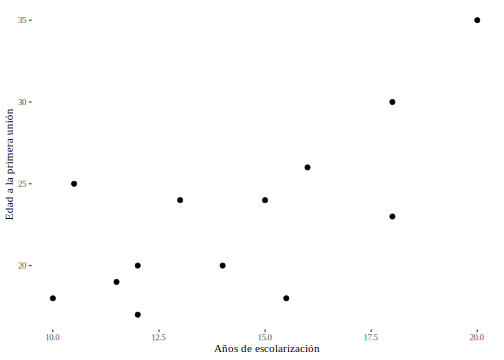
\includegraphics{EstadisticaParaCienciasSocialesConR_files/figure-latex/unnamed-chunk-168-1} 

}

\caption{Obtención gráfica de los puntos de corte que delimitan cinco grupos con igual proporción de casos}\label{fig:unnamed-chunk-168}
\end{figure}

Los quintiles de esta distribución son los siguientes:

\begin{itemize}
\tightlist
\item
  \(P_{20} =\) 7000
\item
  \(P_{40} =\) 12000
\item
  \(P_{60} =\) 16000
\item
  \(P_{80} =\) 21000
\end{itemize}

Y representan valores de ingreso salarial que contienen un quinto de personas asalariadas cada uno. Si alguien está en el primer quintil de los ingresos salariales quiere decir que pertenece al 20\% que tiene los menores ingresos.\\
Una medida de distribución de salarios se obtiene dividiendo dos percentiles extremos, por ejemplo, el percentil 90 dividido el percentil 10. Ese cociente indica cuántas veces más grande es el salario del grupo más alto comparado con el grupo más bajo. En este ejemplo: \[\frac{P_{90}}{P_{10}} =\frac{30000}{4800}=6.25\]

Leemos que el grupo de personas asalariadas de ingresos más altos los tiene \(6.25\) veces superiores a los del grupo de menores ingresos.\\
Esta medida, junto con el coeficiente de Gini y otros cocientes de percentiles, como \(\frac{P_{90}}{P_{50}}\), \(\frac{P_{50}}{P_{10}}\) y \(\frac{P_{80}}{P_{20}}\) se usan para medir el grado de desigualdad en la distribución de los ingresos.

\subsection{Variables métricas: la media o promedio}\label{variables-muxe9tricas-la-media-o-promedio}

Si se ha alcanzado un nivel de medición intervalar o proporcional, es
posible hacer uso de las propiedades\footnote{Propiedades que se agregan a las de las escalas de menor nivel, por lo que modo y mediana pueden calcularse e interpretarse también en las escalas métricas.} que tienen estas escalas.
Recordemos que además de designar y ordenar, las escalas intervalares
conservan las distancias entre observaciones, y las proporcionales
agregan la proporcionalidad de los valores absolutos y el carácter
absoluto del cero. En este nivel los números que representan las
categorías (o valores) pueden tratarse como tales y se puede operar con ellos. Antes de dar una definición de la media o promedio, veamos la idea intuitiva que tenemos, ya que se trata de una medida de mucho uso.
Cuando queremos calcular un promedio ``sumamos y dividimos por la
cantidad de casos''. Así, si tres personas cometen 5, 8 y 12 errores cada una, el promedio de esa variable (número de errores) es
\(\frac{5 + 8 + 12}{3} = \frac{25}{3} = 8.33\). Usaremos la expresión
\(\overline{x}\) para referirnos a la media, con lo que el resultado se
escribe: \(\overline{x} = 8.33\) errores.

¿Cómo extenderemos esta forma de cálculo al caso en que la variable no
está presentada en serie simple sino en distribución de frecuencias?
Recordando que la frecuencia indica la cantidad de veces que cada valor
se repite, por lo que habrá que considerar cada valor tantas veces como
lo indique su frecuencia absoluta simple. Volvamos a la distribución del número de materias aprobadas por estudiantes que cursan segundo año de una carrera universitaria:

\begin{longtable}[]{@{}lc@{}}
\toprule\noalign{}
Número de materias aprobadas & f \\
\midrule\noalign{}
\endhead
\bottomrule\noalign{}
\endlastfoot
0 & 30 \\
1 & 150 \\
2 & 200 \\
3 & 300 \\
4 & 250 \\
5 & 200 \\
6 & 20 \\
Total & 1150 \\
\end{longtable}

El valor 0 (cero) está repetido 30 veces, lo que indica que hay 30
estudiantes que no han aprobado aún ninguna materia. Del mismo modo, 150 aprobaron 1 materia, etc., por lo que si estuvieran presentados
en serie simple, se sumarían los 1150 valores (30 veces el 0, 150 veces
el 1, etc.) y esa suma se dividiría por 1150. Para hacerlo sobre la
distribución de frecuencia, se multiplica cada valor de la variable por
su frecuencia (que es equivalente a sumarlo tantas veces como aparece) y se divide por el total de casos. Resulta:

\[\overline{x} = \frac{0*30 + 1*150 + 2*200 + 3*300 + 4*250 + 5*200 + 6*20}{1150} = 3.10\]

La expresión formal de este cálculo es:

\[\overline{x} = \frac{\sum_{i = 1}^{k}{x_{i}*f_{i}}}{n}\]

En la que:\\
\(x_i\) es cada valor de la variable,\\
\(f_i\) es su frecuencia absoluta simple,\\
\(k\) es el número de categorías y\\
\(n\) es el total de observaciones.

La fórmula indica que cada valor de la variable (\(x_i\))
se multiplica por su frecuencia (\(f_i\)), se suman desde el primero
(\(i=1\)) hasta el último (\(k\)) y el resultado se divide por el total de
casos (\(n\)).

Veamos que no se trató como podríamos haber pensado rápidamente, de
sumar desde el cero hasta el seis y dividir por siete. Haber hecho eso
habría implicado dos errores: el primero es el de no considerar cuántas
veces está repetido cada valor (su frecuencia absoluta simple), el
segundo es el de confundir el número de casos (1150) con el número de
categorías (7). Este último error puede provenir de una confusión entre
la presentación en serie simple o en distribución de frecuencias. Cuando
se observa una serie simple, los valores ``sueltos'' de la variable
coinciden con sus categorías, pero cuando se agrupa, cada categoría
incluye cierta cantidad de casos que tienen el mismo valor, lo cual está
indicado en la frecuencia de cada categoría.

En el ejemplo anterior entonces, el número promedio de materias
aprobadas es 3.10. Este número no es entero y no es un valor que se
pueda observar; nadie tiene 3.10 materias aprobadas. Sin embargo, es
valioso para caracterizar a la distribución completa y para hacer
comparaciones. Por ejemplo, si entre quienes cursan por la mañana la media es de 3.10 materias aprobadas y entre quienes lo hacen por la tarde es de 3.90; puede decirse que el segundo grupo tiene aprobadas, en promedio, más materias que el primero aunque nadie haya aprobado 3.10 ni 3.90 materias.

Por el momento ofreceremos una definición operacional de la media, más
adelante podrá darse una definición conceptual, basada en sus
propiedades.

\begin{longtable}[]{@{}
  >{\centering\arraybackslash}p{(\linewidth - 0\tabcolsep) * \real{1.0000}}@{}}
\toprule\noalign{}
\endhead
\bottomrule\noalign{}
\endlastfoot
La \textbf{media} (o promedio) es un valor de la variable obtenido sumando todas las observaciones multiplicadas por su frecuencia absoluta y dividiendo el resultado en el número total de casos. Se indica como \(\overline{x}\) (equis media). \\
\end{longtable}

Cuando la distribución de frecuencias presenta los datos agrupados,
aparece el problema de no tener un único valor en cada categoría. Por
ejemplo y nuevamente en el caso de los tiempos de reacción medidos entre 34 participantes de un experimento:

\begin{longtable}[]{@{}lc@{}}
\toprule\noalign{}
Tiempo de reacción (en segundos) & f \\
\midrule\noalign{}
\endhead
\bottomrule\noalign{}
\endlastfoot
1.0 - 1.5 & 5 \\
1.5 - 2.0 & 7 \\
2.0 - 2.5 & 6 \\
2.5 - 3.0 & 3 \\
3.0 - 3.5 & 8 \\
3.5 - 4.0 & 5 \\
Total & 34 \\
\end{longtable}

Aquí no hay un valor único en cada categoría, sino un intervalo que
incluye diferentes valores. Esto se resuelve considerando, para cada
intervalo, su \textbf{marca de clase} (el punto medio), que es el promedio de
los extremos de cada intervalo. La siguiente tabla agrega las marcas de
clase de cada intervalo, indicadas como \(x'\):

\begin{longtable}[]{@{}lcc@{}}
\toprule\noalign{}
Tiempo de reacción (en segundos) & x' & f \\
\midrule\noalign{}
\endhead
\bottomrule\noalign{}
\endlastfoot
1.0 - 1.5 & 1.25 & 5 \\
1.5 - 2.0 & 1.75 & 7 \\
2.0 - 2.5 & 2.25 & 6 \\
2.5 - 3.0 & 2.75 & 3 \\
3.0 - 3.5 & 3.25 & 8 \\
3.5 - 4.0 & 3.75 & 5 \\
Total & & 34 \\
\end{longtable}

Ahora puede usarse el método anterior para calcular la media, tomando
las marcas de clase como los valores de la variable:

\[\overline{x} = \frac{1.25*5 + 1.75*7 + 2.25*6 + 2.75*3 + 3.25*8 + 3.75*5}{34} = 2.5\]

Resulta así que el tiempo promedio de reacción es de 2.5 segundos. Este
procedimiento es impreciso, porque asigna a todos los casos que están
dentro de cada categoría el mismo valor (el centro del intervalo) y se
justifica en situaciones en que la única información disponible es la
tabla con los valores agrupados; si se cuenta con la matriz de datos, el
cálculo debe hacerse usando todos los valores observados de la variable,
recurriendo a un software especializado cuando sean muchos datos.

Si bien la media es una medida muy valiosa para resumir un conjunto de
datos, a veces se hace un uso abusivo de ella, al aplicarla a variables
que no tienen el nivel de medición adecuado para autorizar su uso. Un
ejemplo de esto es el caso de las calificaciones escolares, que solo
permiten ordenar a las personas evaluadas según los resultados, pero que no
implican la proporcionalidad de los valores (quien obtiene 10 no sabe el
doble que quien obtiene 5). Aun así, es habitual que se calcule
incorrectamente el ``promedio de las notas''.

\section{La forma de la distribución}\label{la-forma-de-la-distribuciuxf3n}

La media es una medida muy completa como resumen de los datos, ya que los considera a todos con la frecuencia de cada uno. Opera como un punto de equilibrio en un conjunto de datos. Sin embargo esto puede ser una dificultad en algunos tipos de distribución. Consideremos el siguiente
ejemplo simple, que proviene de una matriz de datos ficticia:

\begin{longtable}[]{@{}lc@{}}
\toprule\noalign{}
x & f \\
\midrule\noalign{}
\endhead
\bottomrule\noalign{}
\endlastfoot
3 & 16 \\
4 & 7 \\
5 & 5 \\
6 & 6 \\
10 & 3 \\
Total & 37 \\
\end{longtable}

Estos datos muestran una marcada concentración en el valor 3, donde se
encuentra la mitad de las observaciones. El resto de los valores son
superiores y hay uno extremo, el 10, que tiene poca frecuencia: hay solo
tres observaciones con ese valor. Veamos cuál es el efecto de esta forma
de distribuirse de los datos. La media es:

\[\overline{x} = \frac{3*16 + 4*7 + 5*5 + 6*6 + 10*3}{37} = 4.51\]

A pesar de la concentración en 3 que se observa, la media es superior a 4, que es un resultado contrario a lo que intuitivamente esperaríamos,
porque habríamos supuesto que se ubicaría más cerca de 3, ya que 3
parece ser un valor muy ``representativo'' de esta distribución, sin
embargo, la media da un número bastante más grande. Esto se debe a la
presencia de valores extremos, en este ejemplo el 10. Aunque este número tiene poca frecuencia, su efecto es de ``tirar de la media'' hacia valores más grandes. Esto sucede siempre con la media y proviene de su
característica de tener en cuenta todos los valores de la distribución.
Por esa razón, cuando la distribución se presenta como la anterior, la
media no es una buena medida de centralidad.

El histograma siguiente muestra la forma de la distribución:

\begin{figure}[H]

{\centering 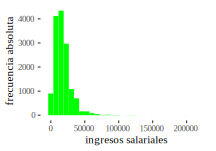
\includegraphics{EstadisticaParaCienciasSocialesConR_files/figure-latex/unnamed-chunk-174-1} 

}

\caption{Visualización de valores atípicos}\label{fig:unnamed-chunk-174}
\end{figure}

En el gráfico se ve el carácter atípico del valor 10, que aparece muy
alejado de la parte principal de la distribución. Decimos en este caso
que la distribución es asimétrica.

Este inconveniente de la media aparece a menudo en las discusiones
salariales por sectores. A menudo se escucha que no se justifica un
aumento porque el salario promedio del sector es de \emph{X pesos}. Argumento al que se contrapone (expresado de diferentes maneras) que ese promedio incluye al personal que tiene salarios muy altos. Se trata de distribuciones asimétricas, que tienen la mayor parte de los casos con salarios bajos o intermedios y unos pocos casos con salarios muy superiores, como lo muestra el histograma siguiente.

\begin{figure}[H]

{\centering 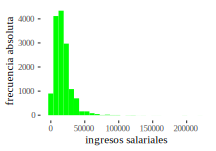
\includegraphics{EstadisticaParaCienciasSocialesConR_files/figure-latex/unnamed-chunk-175-1} 

}

\caption{Distribución de los ingresos salariales}\label{fig:unnamed-chunk-175}
\end{figure}

Por eso cuando se calcula la media se obtiene un resultado que representa mal al conjunto de datos.

\subsection{Asimetría}\label{asimetruxeda}

La \textbf{asimetría} de una distribución se indica señalando hacia dónde se
sitúan los valores extremos. Si, como en los ejemplos anteriores, los valores
extremos son mayores que la mayor parte de los datos, la asimetría es
\textbf{hacia la derecha}.

La asimetría puede ser en sentido opuesto, si hay observaciones
particularmente pequeñas y en ese caso se tratará de una distribución
\textbf{asimétrica hacia la izquierda}. Como en el ejemplo siguiente (datos ficticios):

\begin{longtable}[]{@{}lc@{}}
\toprule\noalign{}
X & F \\
\midrule\noalign{}
\endhead
\bottomrule\noalign{}
\endlastfoot
100 & 5 \\
200 & 10 \\
300 & 20 \\
400 & 20 \\
500 & 50 \\
600 & 70 \\
Total & 175 \\
\end{longtable}

Cuyo histograma es:

\begin{figure}[H]

{\centering 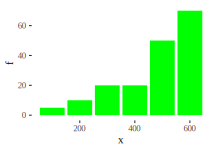
\includegraphics{EstadisticaParaCienciasSocialesConR_files/figure-latex/unnamed-chunk-178-1} 

}

\caption{Ejemplo de distribución asimétrica a la izquierda}\label{fig:unnamed-chunk-178}
\end{figure}

Aquí los valores extremos se encuentran por debajo del grupo principal
de datos y la media se inclinará hacia los valores más pequeños. Así,
aunque la mayoría de los casos se encuentra entre 500 y 600, la media
es:

\[\overline{x} = \frac{100*5 + 200*10 + 300*20 + 400*20 + 500*50 + 600*70}{175} = 477.14\]

Un resultado que está por debajo de esos valores que concentran muchos
casos. Decimos ahora que la asimetría es hacia la izquierda.

Los siguientes histogramas, son ejemplos de formas posibles en cuanto a simetría:

\begin{figure}[H]

{\centering 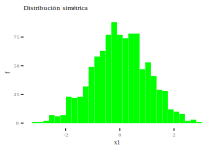
\includegraphics{EstadisticaParaCienciasSocialesConR_files/figure-latex/unnamed-chunk-179-1} 

}

\caption{Histogramas de variables con diferente asimetría}\label{fig:unnamed-chunk-179-1}
\end{figure}
\begin{figure}[H]

{\centering 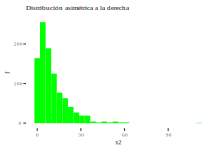
\includegraphics{EstadisticaParaCienciasSocialesConR_files/figure-latex/unnamed-chunk-179-2} 

}

\caption{Histogramas de variables con diferente asimetría}\label{fig:unnamed-chunk-179-2}
\end{figure}
\begin{figure}[H]

{\centering 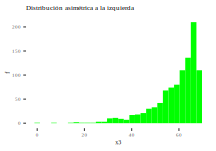
\includegraphics{EstadisticaParaCienciasSocialesConR_files/figure-latex/unnamed-chunk-179-3} 

}

\caption{Histogramas de variables con diferente asimetría}\label{fig:unnamed-chunk-179-3}
\end{figure}

La asimetría puede evaluarse directamente a partir de las medidas de
centralidad, ya que la posición relativa de la media y la mediana
indican hacia dónde ésta sucede. Cuando la media y la mediana coinciden,
la distribución es simétrica, es decir carece de asimetría. Si la media
supera a la mediana, se trata de una distribución asimétrica a la
derecha y si la media es menor que la mediana, la asimetría será hacia
la izquierda.

En estas distribuciones las medias y medianas son:

\begin{itemize}
\tightlist
\item
  x1: media = 0.01, mediana = 0.01
\item
  x2: media = 10.36, mediana = 7.44
\item
  x3: media = 58.68, mediana = 61.75
\end{itemize}

\begin{longtable}[]{@{}
  >{\centering\arraybackslash}p{(\linewidth - 2\tabcolsep) * \real{0.5921}}
  >{\centering\arraybackslash}p{(\linewidth - 2\tabcolsep) * \real{0.4079}}@{}}
\toprule\noalign{}
\begin{minipage}[b]{\linewidth}\centering
Posición relativa de la media y la mediana:
\end{minipage} & \begin{minipage}[b]{\linewidth}\centering
Asimetría de la Distribución:
\end{minipage} \\
\midrule\noalign{}
\endhead
\bottomrule\noalign{}
\endlastfoot
\(\overline{x} = M_{dn}\) & Simétrica \\
\(\overline{x} > M_{dn}\) & Asimétrica a la derecha \\
\(\overline{x} < M_{dn}\) & Asimétrica a la izquierda \\
\end{longtable}

\begin{longtable}[]{@{}
  >{\centering\arraybackslash}p{(\linewidth - 0\tabcolsep) * \real{1.0000}}@{}}
\toprule\noalign{}
\endhead
\bottomrule\noalign{}
\endlastfoot
Una distribución es \textbf{simétrica} si la media coincide con la mediana. La distribución se llama \textbf{asimétrica a la derecha} si la media es mayor que la mediana, y \textbf{asimétrica a la izquierda} si la media es menor que la mediana. \\
\end{longtable}

Las siguientes ojivas de Galton corresponden a las tres distribuciones anteriores. De estos gráficos interesa la zona en que crecen más rápido, porque allí es donde está la mayor concentración de casos. Cuando la distribución es simétrica, la parte de crecimiento rápido (donde la curva tiene a ser más vertical) está al centro, si es asimétrica a la derecha, crece rápido al principio, mientras que cuando es asimétrica a la izquierda, la parte de crecimiento rápido corresponde a los valores más altos de la variable.

\begin{figure}[H]

{\centering 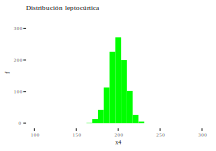
\includegraphics{EstadisticaParaCienciasSocialesConR_files/figure-latex/unnamed-chunk-180-1} 

}

\caption{Ojivas de Galton correspondientes a variables con diferente asimetría}\label{fig:unnamed-chunk-180-1}
\end{figure}
\begin{figure}[H]

{\centering 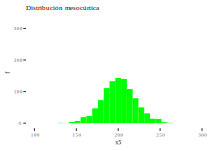
\includegraphics{EstadisticaParaCienciasSocialesConR_files/figure-latex/unnamed-chunk-180-2} 

}

\caption{Ojivas de Galton correspondientes a variables con diferente asimetría}\label{fig:unnamed-chunk-180-2}
\end{figure}
\begin{figure}[H]

{\centering 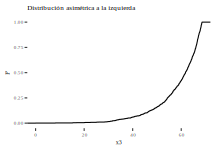
\includegraphics{EstadisticaParaCienciasSocialesConR_files/figure-latex/unnamed-chunk-180-3} 

}

\caption{Ojivas de Galton correspondientes a variables con diferente asimetría}\label{fig:unnamed-chunk-180-3}
\end{figure}

La evaluación cuantitativa de la asimetría de una distribución permite la comparación entre distribuciones en cuanto al grado de asimetría, para indicar cuándo una distribución es más asimétrica que otra. Para hacerlo se usan los \textbf{coeficientes de asimetría}. Estos coeficientes miden dos aspectos
de la asimetría: hacia qué lado sucede y cuán acentuada es. Su signo
positivo indica asimetría hacia la derecha y negativo hacia la
izquierda. El valor absoluto del coeficiente indica si es muy asimétrica
o poco. Por ejemplo, una distribución cuya asimetría vale 1.5 es más
asimétrica que una con coeficiente 1.2, y ambas son asimétricas hacia la
derecha. Cuando la distribución es simétrica, el coeficiente vale cero,
no es positivo ni negativo. Uno de los más frecuentemente usados es el
coeficiente de asimetría de Fisher\footnote{Otros coeficientes de asimetría son: el de Pearson, que compara la ubicación de la media y del modo, y el de Bowley, que compara los cuartiles y la mediana.}, que se calcula como:

\[g_{1} = \frac{\sum_{i = 1}^{n}{\left( x_{i} - \overline{x} \right)^{3}*f_{i}}}{n*s^{3}}\]

Y cuya interpretación es:

\begin{itemize}
\item
  \(g_{1} = 0\) La distribución es simétrica.
\item
  \(g_{1} > 0\) Asimétrica hacia la derecha.
\item
  \(g_{1} < 0\) Asimétrica hacia la izquierda.
\end{itemize}

En la práctica, es improbable que el coeficiente valga exactamente cero,
por lo que se considera simétrica a una distribución cuyo coeficiente
esté entre \(-0.5\) y \(0.5\).

\subsection{Curtosis}\label{curtosis}

Además de la simetría, disponemos de otro indicador de la forma de la
distribución, una medida de cuán ``puntiaguda'' es la curva, se denomina
\textbf{curtosis} y distingue distribuciones con forma estrecha y elevada de que
tienen forma amplia y baja. Como en los siguientes gráficos:

\begin{figure}[H]

{\centering 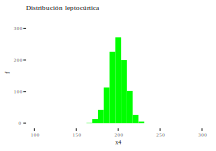
\includegraphics{EstadisticaParaCienciasSocialesConR_files/figure-latex/unnamed-chunk-181-1} 

}

\caption{Histogramas de variables con diferente curtosis}\label{fig:unnamed-chunk-181-1}
\end{figure}
\begin{figure}[H]

{\centering 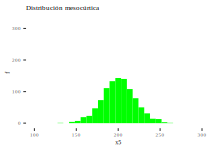
\includegraphics{EstadisticaParaCienciasSocialesConR_files/figure-latex/unnamed-chunk-181-2} 

}

\caption{Histogramas de variables con diferente curtosis}\label{fig:unnamed-chunk-181-2}
\end{figure}
\begin{figure}[H]

{\centering 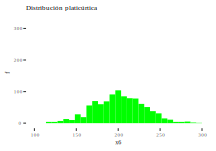
\includegraphics{EstadisticaParaCienciasSocialesConR_files/figure-latex/unnamed-chunk-181-3} 

}

\caption{Histogramas de variables con diferente curtosis}\label{fig:unnamed-chunk-181-3}
\end{figure}

Estos tres ejemplos corresponden a distribuciones simétricas, pero
también pueden ser asimétricas.

La curtosis se mide con un coeficiente específico, que vale cero para
distribuciones mesocúrticas, es negativo para las platicúrticas y
positivo para las leptocúrticas. Su cálculo es:

\[g_{2} = \frac{\sum_{i = 1}^{n}{\left( x_{i} - \overline{x} \right)^{4}*f_{i}}}{n*s^{4}} - 3\]

Su interpretación es:

\begin{itemize}
\item
  \(g_{2} = 0\) La distribución es mesocúrtica
\item
  \(g_{2} > 0\) Leptocúrtica
\item
  \(g_{2} < 0\) Platicúrtica
\end{itemize}

Con datos reales, muy raramente el valor será exactamente cero, por lo
que se trata como mesocúrtica a una distribución cuyo coeficiente se
encuentre entre -0,5 y 0,5.

\subsection{Box-plots}\label{box-plots}

Un gráfico que puede resumir de manera muy compacta la información sobre
una distribución de frecuencias es el que se llama \textbf{diagrama de caja},
o también \textbf{diagrama de caja y bigotes} o \textbf{box-plot}, que fue
propuesto por John Tukey en 1970, pero no se hizo conocido hasta la publicación posterior \citep{tukey77}.
Aplicado a las edades de quienes están cursando en la universidad según la EPH, genera:

\begin{figure}[H]

{\centering 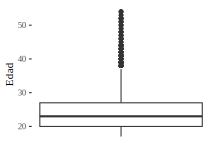
\includegraphics{EstadisticaParaCienciasSocialesConR_files/figure-latex/unnamed-chunk-182-1} 

}

\caption{Box plot de las edades de estudiantes en la universidad}\label{fig:unnamed-chunk-182}
\end{figure}

Este gráfico representa sobre el eje vertical los valores de la variable y muestra una ``caja'' delimitada por los cuartiles 1 y 3. Según la definición de los cuartiles, esa caja contiene al 50\% central de los casos. Dentro de la caja se muestra la mediana en la línea horizontal. Se aprecia la concentración de casos en los valores bajos de la variable y unos pocos casos extremos que acusan la asimetría hacia la derecha de la distribución.

El box-plot es adecuado para comparar grupos, en este ejemplo, se puede incluir la condición de actividad y obtener:

\begin{figure}[H]

{\centering 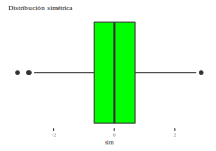
\includegraphics{EstadisticaParaCienciasSocialesConR_files/figure-latex/unnamed-chunk-183-1} 

}

\caption{Box plot de las edades de estudiantes en la universidad, según estado laboral}\label{fig:unnamed-chunk-183}
\end{figure}

Se observa que, aunque en todos los grupos existen casos de estudiantes con edades altas, quienes no tienen actividad laboral (inactives) se concentran en las edades más bajas.

Además de la caja, se ven dos segmentos que se extienden por encima y por debajo de ella. La longitud de estos segmentos (llamados a veces ``bigotes'') depende de una característica de la distribución que se trata en el apartado siguiente: la dispersión.

El box plot puede aparecer presentado de manera vertical u horizontal. Los siguientes corresponden a distribuciones de diferente asimetría.

\begin{figure}[H]

{\centering \includegraphics{EstadisticaParaCienciasSocialesConR_files/figure-latex/unnamed-chunk-184-1} 

}

\caption{Box plots correspondientes a variables de diferente asimetría}\label{fig:unnamed-chunk-184-1}
\end{figure}
\begin{figure}[H]

{\centering \includegraphics{EstadisticaParaCienciasSocialesConR_files/figure-latex/unnamed-chunk-184-2} 

}

\caption{Box plots correspondientes a variables de diferente asimetría}\label{fig:unnamed-chunk-184-2}
\end{figure}
\begin{figure}[H]

{\centering \includegraphics{EstadisticaParaCienciasSocialesConR_files/figure-latex/unnamed-chunk-184-3} 

}

\caption{Box plots correspondientes a variables de diferente asimetría}\label{fig:unnamed-chunk-184-3}
\end{figure}

\section{Medidas de dispersión}\label{medidas-de-dispersiuxf3n}

Además de indicar alrededor de qué valores se distribuyen los datos, también es necesario indicar si se encuentran concentrados alrededor de esos valores (si son cercanos a ellos) o dispersos (si están alejados). Por ejemplo, un promedio de 20 sesiones de psicoterapia puede provenir de cuatro casos que utilizaron 18, 19, 21 y 22 sesiones o de otros cuatro que hayan insumido 5, 10, 30 y 35 sesiones. En la primer situación las cuatro observaciones son cercanas entre sí, están concentradas, mientras que en la segunda están lejos, dispersas. Diremos que en el primer caso la distribución es homogénea o que presenta poca dispersión y en el segundo que es heterogénea o que presenta mucha dispersión.

Conocer esto tiene importancia para poder evaluar la calidad de las medidas de centralidad, en particular de la media. Esto es así porque en una distribución muy dispersa, la media será un promedio de valores muy diferentes entre sí y no será tan fiel a los datos como si estos valores fueran similares. La media de 20 sesiones del primer ejemplo es una mejor medida resumen que la misma media de 20 del segundo, porque la primera refleja mejor los datos de origen. Debido a esto, decimos que en la primera de las situaciones del ejemplo, la media es más \emph{representativa} de los datos de los que proviene.

Nos ocuparemos ahora del modo en que puede medirse esa dispersión, cómo transformarla en una medida resumen que indique brevemente si los datos están dispersos o concentrados.

\subsection{Recorrido}\label{recorrido}

Una primera aproximación al problema es la de considerar la distancia que hay entre los valores extremos, desde el más pequeño hasta el más grande. Si usamos este procedimiento en el ejemplo anterior vemos que en la primera distribución hay 4 unidades entre la primera y la última observación (de 18 a 22) y en la segunda hay 30 unidades de extremo a extremo (de 5 a 35). Por lo que ésta sería una medida de la dispersión.
Esta medida se llama \textbf{recorrido}, se indica con la letra \(R\) y la expresión formal de su cálculo es:

\[R = x_{\max} - x_{\min}\]

Donde \(x_{\max}\) y \(x_{\min}\) representan a los valores máximo y mínimo
respectivamente.\\
En las distribuciones del ejemplo, los recorridos son
\(R=4\) y \(R=30\) respectivamente, que resumen la mayor dispersión de la
segunda.

\begin{longtable}[]{@{}
  >{\centering\arraybackslash}p{(\linewidth - 0\tabcolsep) * \real{1.0000}}@{}}
\toprule\noalign{}
\endhead
\bottomrule\noalign{}
\endlastfoot
Se llama \textbf{recorrido} de una distribución a la diferencia entre los valores máximo y mínimo de la variable. Se indica \(R\). \\
\end{longtable}

Cuando la distribución tiene más casos, el recorrido es insuficiente
como medida de dispersión, ya que está determinado solo por los valores
extremos, sin tener en cuenta los intermedios. Por ejemplo, las dos siguientes series tienen la misma media,
igual a 8:

\[2,\: 8,\: 8,\: 8,\: 8,\: 8,\: 14\]

\[7,\: 8,\: 8,\: 8,\: 8,\: 8,\: 9\]

El recorrido vale 12 para la primera (\(R=14–2\)) y 2 para la segunda
(\(R=9–7\)) es una diferencia muy acentuada aunque las dos distribuciones
solo difieren en los valores extremos. Dicho de otra manera, si sucede
que hay un caso (o unos pocos) que tiene un valor excepcionalmente alto
(o bajo), el recorrido dará un valor alto, indicando gran dispersión, lo
que nos puede hacer pensar que todos los datos están dispersos. Por esa
razón se dice que es una medida ``gruesa'' de la variabilidad de los
datos.

\subsection{Amplitud intercuartílica}\label{amplitud-intercuartuxedlica}

Un modo de afinar la calidad de esta medida es la de tomar la distancia
que hay, no ya entre los valores extremos, sino entre los cuartiles
primero y tercero. La medida que usa esta distancia se llama amplitud
intercuartílica y es simplemente la diferencia entre el tercer cuartil y
el primero:

\[AIQ = Q_{3}{- Q}_{1}\]

Si bien esta medida tampoco considera todas las observaciones -ya que solo tiene en cuenta los dos cuartiles-, es mejor que el recorrido, porque deja de lado los valores extremos, aquellos que pertenecen al 25\% más bajo y al 25\% más alto de la distribución.

\begin{longtable}[]{@{}
  >{\centering\arraybackslash}p{(\linewidth - 0\tabcolsep) * \real{1.0000}}@{}}
\toprule\noalign{}
\endhead
\bottomrule\noalign{}
\endlastfoot
La \textbf{amplitud intercuartílica} es la diferencia entre los cuartiles tercero y primero. Se indica \(AIQ\). \\
\end{longtable}

Gráficamente, esta medida es la altura de la caja del Box-plot (o el ancho si se la dibujó horizontal). Algunos autores prefieren informar como medida de dispersión a la mitad de la distancia entre los cuartiles 1 y 3, a la que se denomina \textbf{semi recorrido intercuartilar}, y se abrevia SRIC. No tiene diferencia conceptual con la AIQ, porque ambas consideran distancia entre cuartiles, solo difieren en la convención de informar la distancia completa (AIC) o su mitad (SRIC).

\begin{longtable}[]{@{}
  >{\centering\arraybackslash}p{(\linewidth - 0\tabcolsep) * \real{1.0000}}@{}}
\toprule\noalign{}
\endhead
\bottomrule\noalign{}
\endlastfoot
El \textbf{semi recorrido intercuartilar} es la mitad de la amplitud intercuartílica. Se indica \(SRIC\). \\
\end{longtable}

Que en el Box-plot representa al mitad de la altura de la caja.

\[SRIC = \frac{Q_{3}{- Q}_{1}}{2}\]

\subsection{Medidas de dispersión basadas en la media}\label{medidas-de-dispersiuxf3n-basadas-en-la-media}

Las medidas de variabilidad que más se usan son las que tienen en cuenta
todas las observaciones, es decir aquellas que están basadas en la
media. Una manera de ver si el conjunto de datos está concentrado o
disperso, consiste en observar la distancia de la media a la que se
encuentra cada observación, luego esas distancias individuales pueden
promediarse y tener una idea global de qué tan lejos están los casos del
promedio. Intentemos hacer eso y veamos qué limitación aparece.

Tomemos un conjunto pequeño de datos, presentado en serie simple:

\[5, \:7,\: 9,\: 11\]

La media es 8, como lo es la mediana, por lo que la distribución es simétrica. No hay modo, ya que todos los valores tienen frecuencia igual a uno.
Hemos elegido así el ejemplo solo para darle simplicidad, no es una
condición necesaria para lo que sigue.

Consideremos las distancias desde cada observación hasta la media,
restando a cada una de ellas el valor 8 (la media):

\begin{longtable}[]{@{}cc@{}}
\toprule\noalign{}
\(x_{i}\) & \(x_{i} - \overline{x}\) \\
\midrule\noalign{}
\endhead
\bottomrule\noalign{}
\endlastfoot
5 & -3 \\
7 & -1 \\
9 & 1 \\
11 & 3 \\
\end{longtable}

Las distancias positivas corresponden a valores superiores a la media y
las negativas a los inferiores, si un valor acertara en la media, su
distancia sería cero. Si sumamos todas las diferencias
\(x_{i} - \overline{x}\), el resultado es cero (\(-3-1+1+3=0\)); además, éstas
son simétricas, como efecto de la forma de la distribución original.
Pero el hecho que la suma sea cero no depende de la distribución, sino que es una propiedad de la media. Por ser la media un punto de equilibrio entre las observaciones, las que se distancian por
encima de ella están compensadas por las que lo hacen por debajo\footnote{Para ver esto, comparemos con el caso de la serie: 3, 4, 6, 7, 23, 45 con media 14,7. Las diferencias entre cada observación y la media son las siguientes:

  \begin{longtable}[]{@{}lllllll@{}}
  \toprule\noalign{}
  \emph{x} & 3 & 4 & 6 & 7 & 23 & 45 \\
  \midrule\noalign{}
  \endhead
  \bottomrule\noalign{}
  \endlastfoot
  \(x_{i} - \overline{x}\) & -11,7 & -10,7 & -8,7 & -7,7 & 8,3 & 30,3 \\
  \end{longtable}

  En este caso las diferencias no son simétricas, pero es igualmente
  cierto que su suma es igual a cero, es decir que están compensadas
  las diferencias por encima y por debajo de la media.}.

Los valores \(x_{i} - \overline{x}\) se llaman \textbf{desvíos}, que indican cuánto
se aleja cada observación de la media. Como vemos, pueden ser positivos o
negativos según se trate de observaciones que superen a la media o que
estén por debajo de ella. Acabamos de ver también que su suma vale cero,
es decir que \(\sum_{i = 1}^{n}{\left( x_{i} - \overline{x} \right) = 0}\)
y que esta es una cualidad de la media, que no depende de los datos\footnote{Puede verse que es así haciendo: \(\sum_{i = 1}^{n}{\left( x_{i} - \overline{x} \right) = \sum_{i = 1}^{n}x_{i} - \sum_{i = 1}^{n}\overline{x}}\), como \(\overline{x}\) es una constante, el segundo término es \(n*\overline{x}\), igual que el primero, según la definición operativa de la media. Por lo tanto la diferencia es cero, cualquiera sea el conjunto de datos.}.

La representación gráfica de esta propiedad puede verse pensando en una analogía física; como si cada caso graficado en el histograma fuese un bloque de cierto peso, situado en el valor de la variable. Con esa idea, la ubicación de la media es el punto donde habría que apoyar el histograma para que éste quede en equilibrio:

\begin{figure}[H]

{\centering \includegraphics{EstadisticaParaCienciasSocialesConR_files/figure-latex/unnamed-chunk-185-1} 

}

\caption{Esquema de la ubicación de la media en el punto de equilibrio del histograma}\label{fig:unnamed-chunk-185}
\end{figure}

El triángulo del gráfico equivale al punto de apoyo que permite el equilibrio de ese ``objeto''.

Tan importante es esta propiedad que la usaremos para dar
una definición más completa de la media:

\begin{longtable}[]{@{}
  >{\centering\arraybackslash}p{(\linewidth - 0\tabcolsep) * \real{1.0000}}@{}}
\toprule\noalign{}
\endhead
\bottomrule\noalign{}
\endlastfoot
La \textbf{media} es el valor de la variable que anula la suma de los desvíos en torno suyo. \\
\end{longtable}

El tema que nos ocupa en este momento es el de medición de la
variabilidad del conjunto de casos, y entonces, la consecuencia de esta propiedad es que no será posible usar la suma de los desvíos como indicador de dispersión, ya que da siempre cero, con datos homogéneos o heterogéneos.

A fin de resolver este problema vamos a eliminar el signo, usando el
hecho que todo número elevado a una potencia par es positivo, sin
importar el signo que haya tenido el número. Elevaremos entonces al
cuadrado cada una de los desvíos y así se perderá su signo y ya no será cero la suma de todos ellos.

\subsection{Varianza}\label{varianza}

Usando ese recurso, definimos la \textbf{varianza\footnote{En este punto aparece la primera diferencia entre cálculos hechos sobre datos de una muestra o de una población. Si estuviésemos trabajando sobre toda la población, la varianza (a la que indicaríamos con otra letra) tendría denominador \(n\), en lugar de \(n-1\). No podemos explicar la razón de esto aún, habrá que esperar al capítulo de estimación. En algunos manuales, a la varianza calculada con denominador \(n-1\) se la llama \emph{cuasivarianza} o también \emph{seudovarianza}.}}, a la que simbolizaremos como \(V(x)\) o más frecuentemente como \(s^2\) de la siguiente forma:

\[s^{2} = \frac{\sum_{i = 1}^{n}\left( x_{i} - \overline{x} \right)^{2}}{n - 1}\]

\begin{longtable}[]{@{}
  >{\centering\arraybackslash}p{(\linewidth - 0\tabcolsep) * \real{1.0000}}@{}}
\toprule\noalign{}
\endhead
\bottomrule\noalign{}
\endlastfoot
Se llama \textbf{varianza} de una distribución a la suma de los cuadrados de los desvíos alrededor de la media, dividida por el total de observaciones menos uno. Se indica \(s^2\). \\
\end{longtable}

Es una medida muy valiosa de la dispersión que tiene un conjunto de
datos, cuanto mayor es, tanto más dispersos éstos se encuentran, es
decir, son más heterogéneos. No puede ser negativa, porque es una suma de cuadrados y solo es cero si todos los desvíos son cero, es decir si todas las observaciones coinciden con la media\footnote{En este caso no hay variabilidad, y en consecuencia, no hay variable, porque el valor asumido es siempre el mismo. Se trata de una constante.}.

Hay tres propiedades de la varianza que señalaremos porque serán
necesarias más adelante:

-La varianza de una constante es cero. Esto resulta claro ya que la
varianza mide la dispersión y si todas las observaciones son iguales no hay dispersión:

\[V\left( k \right) = 0\]

-La varianza de una constante que multiplica a una variable es la
constante elevada al cuadrado multiplicada por la varianza de la
variable:

\[V\left( k*x \right) = k^{2}*V(x)\]

-La varianza de la suma de dos variables independientes (este concepto se trata más adelante) es la suma de
las varianzas de cada una de ellas:

\[V\left( x + y \right) = V\left( x \right) + V(y)\]

A los fines de la interpretación, la varianza presenta dos
inconvenientes. Uno es que sus unidades están elevadas al cuadrado; por lo que, si medimos \emph{número de errores}, la varianza quedará expresada en \emph{número de errores al cuadrado} una entidad que no tiene significado, como tampoco lo tienen \emph{hijos o hijas al cuadrado} para la fecundidad, \emph{pesos al cuadrado} para ingresos o \emph{segundos al cuadrado} para los tiempos de reacción.

El otro inconveniente es que no tiene límite superior, puede ser muy
grande y no tenemos con qué compararla para saber si indica una gran
variabilidad o si es grande porque los valores de la variable lo son.

\subsection{Desviación estándar}\label{desviaciuxf3n-estuxe1ndar}

Para resolver el primer inconveniente, definiremos una medida derivada de la varianza, que se denomina \textbf{desviación estándar} (en algunos textos y programas de análisis de datos es llamada desviación típica). Esta medida, indicada con la letra \(s\) es la raíz cuadrada de la varianza:

\[s = \sqrt{\frac{\sum_{i = 1}^{n}\left( x_{i} - \overline{x} \right)^{2}}{n - 1}}\]

O más simplemente:

\[s = \sqrt{s^{2}}\]

\begin{longtable}[]{@{}
  >{\centering\arraybackslash}p{(\linewidth - 0\tabcolsep) * \real{1.0000}}@{}}
\toprule\noalign{}
\endhead
\bottomrule\noalign{}
\endlastfoot
La \textbf{desviación estándar} es la raíz cuadrada de la varianza. Se indica \(s\). \\
\end{longtable}

Ahora, por el sencillo trámite de introducir una raíz cuadrada, las
unidades de \emph{s} son las mismas que las de la variable original y se resuelve el primer problema.

\subsection{Coeficiente de variación}\label{coeficiente-de-variaciuxf3n}

Para hacer frente al segundo problema, la magnitud de la varianza y la comparación de la dispersión entre medidas expresadas en diferentes unidades ─que sigue siéndolo para la desviación estándar─, definimos una medida relativa de la dispersión: el \textbf{coeficiente de variación}, indicado como CV como el cociente entre la desviación estándar y la media:

\[CV=\frac{s}{\overline{x}}*100\]

Esta medida carece de unidades, porque la media tiene las mismas que las de la desviación estándar, por lo que se trata de una medida relativa de la dispersión. Indica la importancia relativa de la desviación estándar respecto de la media. El factor 100 que acompaña al cociente cumple la función de expresarlo como porcentaje, por comodidad para la lectura.

\begin{longtable}[]{@{}
  >{\centering\arraybackslash}p{(\linewidth - 0\tabcolsep) * \real{1.0000}}@{}}
\toprule\noalign{}
\endhead
\bottomrule\noalign{}
\endlastfoot
El \textbf{coeficiente de variación} expresa de manera relativa la dispersión, midiendo el peso de la desviación estándar comparado con la media. Se indica \(CV\). \\
\end{longtable}

Conocer la dispersión de una distribución de frecuencias es muy
necesario para poder decidir si la media es una medida adecuada para
resumir los datos, y esto no sucede si hay mucha dispersión. Para
aclarar esto veamos un ejemplo: sea un grupo de seis persona que hacen un test y que obtienen los siguientes puntajes: 2, 2, 2, 2, 10, 10. Si calculamos la media obtenemos 4.7. Este número no representa lo que sucede con las seis personas, las cuales tuvieron resultados muy dispares: cuatro de ellas obtuvieron 2 y las otras dos, 10. Si calculamos el CV, resultado es 88.5\%, un valor muy elevado, indicativo que la media no es una medida adecuada para sintetizar al conjunto de datos.\\
Muchas de las críticas mal fundadas hacia la Estadística se equivocan por ignorancia, porque calculan la media cuando no corresponde usarla, o sin hacer referencia a la dispersión entre las observaciones.

En la práctica se considera que si el coeficiente de variación es menor al 10\% (algunas referencias ponen como límite al 15\%), la distribución tiene poca dispersión y entonces podemos confiar en la media como medida de centralidad y tratarla como representativa de los datos que resume. Si el CV supera estos valores, la media no alcanza para resumir los datos y es necesario acompañarla de otras medidas, como la mediana, los cuartiles, el mínimo y máximo.

Calcularemos por única vez las medidas de dispersión de manera manual
para un pequeño conjunto de datos, a fin de seguir de cerca las
operaciones que involucra. Se trata de seis casos clínicos diagnosticados de depresión a partir de cinco o más de los síntomas que indica el manual DSM IV\footnote{Presencia de cinco (o más) de los siguientes síntomas durante un período de 2 semanas, que representan un cambio respecto a la actividad previa; uno de los síntomas debe ser (textualmente):

  1. Estado de ánimo depresivo la mayor parte del día, casi cada día según
  lo indica el propio sujeto (p.~ej., se siente triste o vacío) o la
  observación realizada por otros (p.~ej., llanto). En los niños y
  adolescentes el estado de ánimo puede ser irritable

  2. Disminución acusada del interés o de la capacidad para el placer en
  todas o casi todas las actividades, la mayor parte del día, casi cada
  día (según refiere el propio sujeto u observan los demás)

  3. Pérdida importante de peso sin hacer régimen o aumento de peso (p.
  ej., un cambio de más del 5\% del peso corporal en 1 mes), o pérdida o
  aumento del apetito casi cada día. Nota: En niños hay que valorar el
  fracaso en lograr los aumentos de peso esperables

  4. Insomnio o hipersomnia (sueño excesivo) casi cada día.

  5. Agitación o enlentecimiento psicomotores casi cada día (observable
  por los demás, no meras sensaciones de inquietud o de estar enlentecido)

  6. Fatiga o pérdida de energía casi cada día

  7. Sentimientos de inutilidad o de culpa excesivos o inapropiados (que
  pueden ser delirantes) casi cada día (no los simples autorreproches o
  culpabilidad por el hecho de estar enfermo)

  8. Disminución de la capacidad para pensar o concentrarse, o indecisión,
  casi cada día (ya sea una atribución subjetiva o una observación ajena)

  9. Pensamientos recurrentes de muerte (no sólo temor a la muerte),
  ideación suicida recurrente sin un plan específico o una tentativa de
  suicidio o un plan específico para suicidarse} y que para cada uno de ellos observamos (como variable) el número de síntomas que condujeron al diagnóstico:

\begin{longtable}[]{@{}
  >{\centering\arraybackslash}p{(\linewidth - 6\tabcolsep) * \real{0.0671}}
  >{\centering\arraybackslash}p{(\linewidth - 6\tabcolsep) * \real{0.2013}}
  >{\centering\arraybackslash}p{(\linewidth - 6\tabcolsep) * \real{0.2282}}
  >{\centering\arraybackslash}p{(\linewidth - 6\tabcolsep) * \real{0.5034}}@{}}
\toprule\noalign{}
\begin{minipage}[b]{\linewidth}\centering
Caso
\end{minipage} & \begin{minipage}[b]{\linewidth}\centering
\(x_{i}\) (número de síntomas)
\end{minipage} & \begin{minipage}[b]{\linewidth}\centering
\(x_{i} - \overline{x}\) (desvíos)
\end{minipage} & \begin{minipage}[b]{\linewidth}\centering
\({{(x}_{i} - \overline{x})}^{2}\) (cuadrados de los desvíos)
\end{minipage} \\
\midrule\noalign{}
\endhead
\bottomrule\noalign{}
\endlastfoot
1 & 5 & -2 & 4 \\
2 & 6 & -1 & 1 \\
3 & 6 & -1 & 1 \\
4 & 8 & 1 & 1 \\
5 & 8 & 1 & 1 \\
6 & 9 & 2 & 4 \\
\end{longtable}

\[\overline{x} = \frac{5 + 6 + 6 + 8 + 8 + 9}{6} = 7\]

\[\sum_{i = 1}^{6}{\left( x_{i} - \overline{x} \right)^{2} = 4 + 1 + 1 + 1 + 1 + 4 = 12}\]

\[s^{2} = \frac{\sum_{i = 1}^{6}\left( x_{i} - \overline{x} \right)^{2}}{n - 1} = \frac{12}{6 - 1} = 2.4\]

\[s = \sqrt{s^{2}} = \sqrt{2.4} = 1.55\]

\[CV = \frac{s}{\overline{x}}*100 = \frac{1.55}{7}*100 = 22.13\%\]

La lectura de este resultado es que, para el conjunto de seis personas a las que se observa, el número promedio de síntomas a través de los
cuales es diagnosticada la depresión es de siete. Sin embargo este
número de síntomas es bastante variable según los casos y,
seguramente también entre terapeutas.

\subsection{Box-plots y dispersión}\label{box-plots-y-dispersiuxf3n}

La observación del diagrama de caja (box-plot) nos da también indicios acerca de la dispersión de la variable que se analiza. Cuando la caja es larga estamos en presencia de distribuciones muy dispersas en la parte central, los cuartiles están lejanos, hay mucha amplitud intercuartilar.
Mientras que si la caja es corta, se trata de una concentración de datos
de la parte central de la distribución. La longitud de los bigotes
señala la mayor o menor concentración de los datos en las zonas
extremas. Como dijimos antes, el box-plot es un gráfico que ayuda a
explorar los datos, a hacerse una idea inicial de la distribución y esto puede ser muy valioso cuando se trata de interpretarlos, porque permite sugerir hipótesis que expliquen la distribución que se observa.\\
Haciendo uso de la amplitud intercuartílica estableceremos criterios
para detectar valores que destaquen por alejarse sustancialmente del
grupo mayoritario. Se trata de identificar mediciones atípicas o excepcionalmente
extremas, por ser excesivamente grandes o excesivamente pequeñas. Reconocer estos valores es importante en la etapa exploratoria
de los datos porque obliga a mirarlos en detalle. Puede tratarse de errores de medición o bien de un caso (o unos pocos) que se aparta de
manera excepcional del grupo y que merece un análisis más detallado y
particularizado.

\citet{tukey77} analiza la distancia de los casos a los cuartiles y sugiere
tratar como ``lejanas'' a las observaciones que se encuentren a más de una
amplitud intercuartílica y media (\(1.5*AIQ\)) por debajo del primer
cuartil o por encima del tercero, pero a menos de tres veces la amplitud
intercuartílica (\(3*AIQ\)). Además, aquellas observaciones que estén más
allá de tres AIQ por debajo del primer cuartil o por encima del tercero
se denominan ``muy lejanas''. Este criterio determina entonces zonas en
las que pueden hallarse las observaciones que componen el \(50\%\) que queda fuera de la caja y, según en cuál de ellas se
encuentren, se las identifica como ``cercanas'', ``lejanas'' o ``muy
lejanas''. Las zonas son las siguientes:

\begin{itemize}
\tightlist
\item
  Cercanas:

  \begin{itemize}
  \tightlist
  \item
    Por debajo: entre \(Q_1\) y \(Q_1-1.5*AIQ\)\\
  \item
    Por encima: entre \(Q_3\) y \(Q_3+1.5*AIQ\)
  \end{itemize}
\item
  Lejanas:

  \begin{itemize}
  \tightlist
  \item
    Por debajo: entre \(Q_1-1.5*AIQ\) y \(Q_1-3*AIQ\)\\
  \item
    Por encima: entre \(Q_3+1.5*AIQ\) y \(Q_3+3*AIQ\)
  \end{itemize}
\item
  Muy lejanas:

  \begin{itemize}
  \tightlist
  \item
    Por debajo: menores que \(Q_1-3*AIQ\)\\
  \item
    Por encima: Mayores que \(Q_3+3*AIQ\)
  \end{itemize}
\end{itemize}

La división en zonas puede verse más claramente en un box-plot. En ese gráfico se toma la distancia entre los cuartiles tercero y
primero (la amplitud intercuartílica) como unidad de medida, luego se calcula una vez y media esa medida (\(1.5*AIQ\)) y tres veces esa
medida (\(3*AIQ\)) como puntos de corte para decidir cuándo una observación se aleja excepcionalmente del grupo. Los segmentos del box plot se cortan si se alcanza el máximo de la distribución (hacia arriba) o el mínimo (hacia abajo). Así, los segmentos tienen una longitud que es o bien \(1.5*AIQ\) o bien la distancia hasta el máximo o mínimo.

\begin{figure}[H]

{\centering \includegraphics{EstadisticaParaCienciasSocialesConR_files/figure-latex/unnamed-chunk-187-1} 

}

\caption{Ubicación visual de observaciones lejanas por medio del box plot}\label{fig:unnamed-chunk-187}
\end{figure}

Los puntos que se ven más allá de los segmentos, son tratados como ``lejanos'', porque están más allá de \(1.5*AIQ\) del primero o del tercer cuartil.

\subsection{Medida de la dispersión cuando no hay distancias}\label{medida-de-la-dispersiuxf3n-cuando-no-hay-distancias}

Todo lo indicado hasta el momento acerca de la variabilidad ha
necesitado de la medición de la distancia entre las observaciones: desde el comienzo hablamos de cercanía o lejanía entre los datos. Por lo tanto,
estas medidas, desde el recorrido hasta el coeficiente de variación,
solo tienen sentido si la variable es de nivel intervalar o
proporcional. Si la variable tiene nivel nominal u ordinal habrá que
medir su variabilidad de otra forma. En estos casos cambia un poco el
significado de la variabilidad, ya que estaremos en presencia de una
variable más dispersa cuanto más \emph{equitativamente} se distribuya el
total de observaciones entre las distintas categorías. Por ejemplo, si cien participantes de un experimento se clasifican según cómo sea su rendimiento en una prueba dada, en: muy bueno, bueno, regular, insatisfactorio; la distribución tendrá más
dispersión si 25 casos se encuentran en cada categoría que si la gran
mayoría está en una sola. La distribución:

\begin{longtable}[]{@{}lcc@{}}
\toprule\noalign{}
Rendimiento & f & f' \\
\midrule\noalign{}
\endhead
\bottomrule\noalign{}
\endlastfoot
Muy bueno & 25 & 0.25 \\
Bueno & 25 & 0.25 \\
Regular & 25 & 0.25 \\
Insatisfactorio & 25 & 0.25 \\
Total & 100 & 1.00 \\
\end{longtable}

Tiene más dispersión que esta otra:

\begin{longtable}[]{@{}lcc@{}}
\toprule\noalign{}
Rendimiento & f & f' \\
\midrule\noalign{}
\endhead
\bottomrule\noalign{}
\endlastfoot
Muy bueno & 5 & 0.05 \\
Bueno & 80 & 0.80 \\
Regular & 5 & 0.05 \\
Insatisfactorio & 10 & 0.10 \\
Total & 100 & 1.00 \\
\end{longtable}

¿Por qué? Porque en la segunda, los casos están muy concentrados en una categoría (bueno), mientras que en la primera se dispersan entre todas.

Notemos que ahora habrá más dispersión cuanto más parecidas sean las
frecuencias entre sí. Esto puede parecer contradictorio con lo indicado
para variables cuantitativas, pero allí la mayor dispersión viene dada
por la mayor disparidad entre los valores de las variables, que no puede
evaluarse con variables nominales u ordinales.

Esta forma de considerar la dispersión equivale a la idea de
incertidumbre. Supongamos que conocemos que la distribución del
rendimiento es como lo muestra la primera tabla y que debemos ``adivinar''
cuál es el rendimiento de una persona elegida al azar. No tenemos
ninguna razón para creer de manera preferencial que la persona sea de
rendimiento muy bueno, bueno, regular o insatisfactorio; ya que todos
son igualmente posibles. En esta situación, la incertidumbre es
completa. Por el contrario, si supiéramos que la distribución es la que
muestra la segunda tabla, tenderíamos con justa razón a creer que hay
más chances que la persona elegida al azar tenga rendimiento bueno, ya
que es bastante más probable que pertenezca a esa categoría que a otra.
Diremos que aquí tenemos menos incertidumbre. En el caso extremo que la totalidad de los casos estuviera en la categoría ``bueno'', ya no hay incertidumbre, cualquier persona elegida al azar tendrá ese rendimiento; la incertidumbre es cero, pero ya no es una variable, porque solo tiene una categoría con casos, es una constante y allí la dispersión siempre es cero.

La medida para expresar de manera sintética esta dispersión es:

\[H\left( x \right) = - \sum_{i = 1}^{k}{{f'}_{i}^{}*log{f'}_{i}^{}}\]

Esta medida se llama \emph{entropía de Shannon}, \citet{shannon1948}. El cálculo consiste en multiplicar cada frecuencia relativa por su
propio logaritmo y sumar para todas las categorías. El resultado de la
sumatoria siempre es negativo, por lo que la fórmula incluye un signo
menos para volverlo positivo. Este coeficiente expresa en un solo número
la magnitud de la dispersión. Cuanto más pequeña sea esta medida, tanto
menos dispersa (o más concentrada) será la distribución de la variable
que se analiza.

Aplicado a las dos tablas de más arriba resulta, para la primera:

\[H\left( x \right) = - (0.25*log(0.25) + 0.25*log(0.25) +\] \[0.25*log(0.25) + 0.25*log(0.25)) = - \left( - 0.60 \right) = 0.60\]

Y, para la segunda:

\[H\left( x \right) = - (0.05*log(0.05) + 0.80*log(0.80) +\] \[0.05*log(0.05) + 0.10*log(0.10)) = - \left( - 0.31 \right) = 0.31\]

Así, a la distribución en la que las frecuencias están más concentradas,
es decir la que tiene menor dispersión, le corresponde un menor valor de \(H(x)\).

Cuando la variable tiene solo dos categorías, la proporción de casos en una de ellas es el complemento a uno de la otra, si en una categoría la proporción es \(p\) en la otra será \(1-p\). La máxima concentración se da cuando todos los casos están en una sola categoría, \(p=1\) y \(1-p=0\), allí la dispersión vale cero, porque se trata de una constante: a todos los individuos les corresponde el mismo valor de la variable. La máxima dispersión sucede cuando la distribución entre las dos categorías es equitativa, es decir cuando la mitad de los casos está en cada una: \(p=0.5\) y \(1-p=0.5\).
La medida de esta variabilidad también se llama varianza, pero su cálculo es muy diferente del caso de variables cuantitativas. Para una variable nominal de dos categorías (dicotómica), y un conjunto de \(n\) observaciones, la varianza es:

\[s^2 = p*(1-p)\]

Que alcanza su mínimo en cero cuando todos los casos están en una sola categoría y su máximo en \(0.25\) cuando se distribuyen mitad en cada una.\\
La desviación estándar es: \[s=\sqrt{p*(1-p)}\] Cuyo máximo es \(\sqrt{0.5*0.5}=0.5\)

\section{El individuo en relación a su grupo}\label{el-individuo-en-relaciuxf3n-a-su-grupo}

Un uso muy frecuente de las medidas que acabamos de ver es que permiten decidir si un \emph{valor particular} está cerca o lejos del promedio, o bien si se sitúa o no en los extremos de una distribución. Un valor particular en este caso se
refiere al valor de la variable en un \emph{caso}, por
ejemplo, el puntaje que una persona obtiene en una prueba, el ingreso de un hogar, la PBI per cápita de un país. Así formulado
el problema puede parecer muy elemental, porque puede ``verse'' si un
número está cerca o lejos de otro. Si sabemos que una persona tiene dos metros de estatura, no necesitamos hacer cuentas para saber que es alto, más alto que la mayoría de las personas. Sin embargo, en el caso de medidas menos familiares, a veces resulta difícil hacer juicios de distancia sobre valores absolutos. Si un país tiene PBI per cápita de U\$S20000, hace falta conocer más datos para evaluarlo como alto o bajo.\\
Si sabemos que en una prueba de memoria con un puntaje máximo de 100
puntos, una persona logró 80 puntos, ¿es evidencia para decir que obtuvo un puntaje alto? La respuesta es no, porque no sabemos qué
puntajes obtuvieron las demás personas que hicieron la prueba. Si la
media del grupo completo hubiese sido 60 puntos, entonces 80 sería un
valor elevado, pero si la media hubiese sido de 85, entonces el caso que estamos considerando se encontraría por debajo del promedio. Más aún, si el promedio fuese 60 y la mayoría de las personas evaluadas hubiese obtenido puntajes cercanos a 60 (poca variabilidad), entonces el valor 80 podría considerarse como muy elevado. Solo conocer su puntaje individual no nos dice nada acerca de la posición de un sujeto particular. Dos ejemplos:

\begin{itemize}
\item
  Nos informan que un niño obtuvo un puntaje bruto de 85 en
  la escala de desarrollo infantil de Bayley \citep{Ballot2017}, no tenemos, en principio ningún criterio para decidir si ese puntaje es alto o bajo.
\item
  El Índice de Democracia \citep{demindex2011} de un país es 6.5. ¿Dónde se ubica este país en el conjunto de democracias del mundo? ¿Es alto, medio\ldots?
\end{itemize}

Para situaciones como éstas, muy frecuentes en evaluaciones
cuantitativas, será necesario conocer cuál es la posición \emph{relativa} que un puntaje ocupa respecto del conjunto completo de observaciones.

Supongamos que se aplica una prueba de ortografía a una muestra de
quienes están cursando tercer grado de la escuela primaria, que la media de errores de todo el grado es 10
(\(\overline{x} = 10\) errores) y que la desviación estándar es de 4
(\(s = 4\) errores). Si alguien comete 6 errores en una prueba (\(x = 6\) errores),
podemos decir que cometió menos errores que el promedio del grupo. El
cálculo de la diferencia entre \(x\) y \(\overline{x}\) da \(-4\) errores
(\(x - \overline{x} = 6 - 10 = - 4\)), este resultado nos informa que ese caso se ubica a 4 errores por debajo del promedio (por debajo queda expresado en el signo menos el resultado). Ésta es una medida concreta, ya que expresa el número de errores que separan a esa persona del comportamiento resumido del grupo, Dicho de otra manera, se está midiendo la distancia a que se encuentra el caso particular de la media del conjunto completo: menos cuatro errores. Si ahora a esta diferencia la dividimos por la desviación estándar obtenemos \(-1\) (procedente de \(\frac{- 4\ }{\ \ 4\ }\)), que ya no tiene unidades, es un número abstracto. Como la desviación estándar es de 4 errores y ese caso se encuentra a cuatro errores de la media, esto equivale a decir que esa persona se encuentra ``a una desviación estándar por debajo del promedio''.\\
La operación que hemos hecho ha sido la de restar al valor particular
(de ese caso) la media del grupo y dividir el resultado en la desviación estándar, también del grupo. Hemos calculado lo siguiente:

\[\frac{x - \overline{x}}{s}\]

Este número, que como dijimos no tiene unidades, es diferente para cada valor de \(x\), y mide la distancia a la que se encuentra una observación particular (\(x\)) de la media (\(\overline{x}\)), expresada como fracción de la desviación estándar (\(s\)). Decimos que se trata de una medida \emph{estandarizada} del alejamiento que tiene una observación particular del promedio del conjunto de observaciones. Esta medida expresa el puntaje bruto (en las unidades que sean) en términos de desviaciones estándar.\\
La variable que resulta de esta operación se llama \textbf{desvío estándar}, ya que se trata de un desvío (calculado en la diferencia \(x - \overline{x}\)) expresado como cantidad de desviaciones estándar. Se utiliza la letra \(z\) para indicarla, así:

\[z = \frac{x - \overline{x}}{s}\]

Debido a que la letra \(z\) se utiliza de manera universal para indicar el resultado de esta operación, se lo conoce como \textbf{puntaje z} o \textbf{puntuación z}. Esta nueva variable tiene media igual a cero y desviación estándar igual a uno\footnote{Dado que \(\overline{x}\) y s son constantes, aplicando las
  propiedades de la media, resulta:

  \[\overline{z} = \overline{\left( \frac{x - \overline{x}}{s} \right)} = \frac{\overline{x} - \overline{x}}{s} = 0\]

  También haciendo uso de las propiedades de la varianza, la de z es:

  \[V\left( z \right) = V\left( \frac{x - \overline{x}}{s} \right) = \frac{1}{s^{2}}\left( V\left( x \right) - V\left( \overline{x} \right) \right) = \frac{1}{s^{2}}\left( V\left( x \right) - 0 \right) = \frac{1}{s^{2}}V\left( x \right) = 1\]

  ya que la media es constante por lo que tiene varianza nula, y \(V\left( x \right) = s^{2}\).}.

Volvamos sobre el ejemplo del número de síntomas en que se basa el
diagnóstico de depresión, cuya media fue de 7 y su desviación estándar
de 1.55.

\begin{longtable}[]{@{}
  >{\centering\arraybackslash}p{(\linewidth - 6\tabcolsep) * \real{0.1020}}
  >{\centering\arraybackslash}p{(\linewidth - 6\tabcolsep) * \real{0.3061}}
  >{\centering\arraybackslash}p{(\linewidth - 6\tabcolsep) * \real{0.3469}}
  >{\centering\arraybackslash}p{(\linewidth - 6\tabcolsep) * \real{0.2449}}@{}}
\toprule\noalign{}
\begin{minipage}[b]{\linewidth}\centering
Caso
\end{minipage} & \begin{minipage}[b]{\linewidth}\centering
\(x_{i}\) (número de síntomas)
\end{minipage} & \begin{minipage}[b]{\linewidth}\centering
\(x_{i} - \overline{x}\) (desvíos)
\end{minipage} & \begin{minipage}[b]{\linewidth}\centering
\(z\) (desvíos estándar)
\end{minipage} \\
\midrule\noalign{}
\endhead
\bottomrule\noalign{}
\endlastfoot
1 & 5 & -2 & -1.29 \\
2 & 6 & -1 & -0.65 \\
3 & 6 & -1 & -0.65 \\
4 & 8 & 1 & 0.65 \\
5 & 8 & 1 & 0.65 \\
6 & 9 & 2 & 1.29 \\
\end{longtable}

La última columna proviene de haber dividido cada desvío en la
desviación estándar (1.55). Los desvíos indican a cuántas unidades de la variable (en este ejemplo, \emph{número de síntomas}) se ubica cada caso del promedio. Los desvíos estándar indican a cuántas desviaciones estándar se encuentra cada caso del promedio. El primer diagnóstico está 1.29 desviaciones estándar por debajo del promedio, el segundo y el tercero está a 0.65 desviaciones estándar por debajo del promedio, etc. Los que se ubican por encima del promedio tienen \(z\) positivo.

Para variables nominales, se procede de la misma manera, solo cambia el cálculo de la desviación estándar:\\
Si en un país ``A'' se encuentra que el 12.5\% de la muestra consultada cree que da lo mismo un gobierno autoritario que uno democrático (pregunta P8STGBS de Latinobarómetro 2017) ¿es mucho o poco? Para saberlo necesitamos conocer el porcentaje general de esta respuesta en el conjunto de países que se observaron: este valor es, para los países que participan del estudio, 27.6\%. Ahora se sabe que en el país ``A'' la proporción de quienes creen que da lo mismo el tipo de gobierno es más baja que en el conjunto de países de la región. ¿Cuánto más baja? Se requiere indicar su posición relativa, y eso se hace en términos de puntaje \(z\). La varianza de esta variable se calcula como \[p*(1-p)=0.276*(1-0.276)=0.1998\] y la desviación estándar como \[\sqrt{0.1998}=0.447\].\\
Entonces \(z = \frac{0.125-0.276}{0.447}=-0.34\).\\
Que indica que ese país esta \emph{levemente} por debajo del conjunto. En los próximos capítulos avanzaremos en el análisis de los puntajes \(z\).

Cuando se trata de variables de nivel ordinal también es posible ubicar de manera relativa cada valor de la variable, aunque no puedan medirse distancias, porque pueden calcularse cuantiles e indicar a cuál corresponde cada valor. Antes vimos el modo de señalar gráficamente la ubicación de los cuantiles, allí buscamos de identificar el valor de la variable que corresponde, por ejemplo, al cuantil \(0.90\) ó a cualquier otro. Podemos hacer también el recorrido inverso: dado un valor de la variable ¿a qué cuantil corresponde?

Consideremos los siguientes puntajes brutos obtenidos en una prueba
psicológica administrada a una muestra de \(310\) personas:

\begin{longtable}[]{@{}lccc@{}}
\toprule\noalign{}
x & f & F & F' \\
\midrule\noalign{}
\endhead
\bottomrule\noalign{}
\endlastfoot
20-29 & 0 & 0 & 0.00 \\
30-39 & 10 & 10 & 0.03 \\
40-49 & 30 & 40 & 0.13 \\
50-59 & 50 & 90 & 0.29 \\
60-69 & 70 & 160 & 0.52 \\
70-79 & 90 & 250 & 0.81 \\
80-89 & 40 & 290 & 0.94 \\
90-99 & 10 & 300 & 0.97 \\
100-109 & 5 & 305 & 0.98 \\
110-119 & 5 & 310 & 1.00 \\
Total & 310 & & \\
\end{longtable}

Con las fórmulas para el cálculo o solicitándoles a un software, se obtienen algunos cuantiles de esta distribución. Por ejemplo, \(P_{20}\), \(P_{60}\) y \(P_{90}\) son:

\begin{verbatim}
##  P20  P60  P90 
## 54.5 74.5 84.5
\end{verbatim}

Procediendo del mismo modo, se realiza la siguiente correspondencia de puntajes brutos a deciles (o multiplicados por 10, percentiles:

\begin{longtable}[]{@{}cc@{}}
\toprule\noalign{}
Percentil & X \\
\midrule\noalign{}
\endhead
\bottomrule\noalign{}
\endlastfoot
10 & 47.0 \\
20 & 54.5 \\
30 & 60.4 \\
40 & 64.9 \\
50 & 69.3 \\
60 & 74.5 \\
70 & 76.3 \\
80 & 79.8 \\
90 & 84.5 \\
\end{longtable}

La tabla nos informa sobre los valores de la variable donde se divide
cada 10\% del total de casos. Usando la definición de los deciles
diremos que:

\begin{itemize}
\tightlist
\item
  El 10\% de las personas obtuvo 47 puntos o menos.
\item
  El 20\% obtuvo 54.5 puntos o menos y así para el resto.
\end{itemize}

Con esta información sabemos que si una persona obtuvo 50 puntos, tiene
un puntaje muy bajo, porque supera a menos del 20\% del grupo. O dicho de
otra manera, más del 80\% de las personas alcanzaron puntajes más altos
que aquella. Por el contrario si alguien obtuvo 88 puntos, tiene un puntaje
muy alto, ya que supera al decil 9 (percentil 90), con lo que menos del 10\% del
grupo lo supera. O bien, él supera a más del 90\%.\\
De este modo, la construcción de una tabla en la que se indica el valor
de la variable (el puntaje en la prueba) correspondiente a cada
cuantil, permite conocer si un puntaje dado se ubica en algún extremo
de la distribución (si es excepcionalmente elevado o bajo) o si es un
valor intermedio.

Estas tablas de correspondencia entre valores absolutos (o puntajes
brutos) y los correspondientes valores relativos pueden también
construirse a partir de los desvíos estándar, para lo que se debe
transformar cada valor observado en su puntuación \(z\). Para el ejemplo
anterior se debe calcular la media y la desviación estándar, que dan:
\(\overline{x} = 68.4\) y \(s = 15.7\). Con esto se indican los puntajes \(z\)
que corresponden a cada puntaje bruto, con la transformación
\(z = \frac{x - \overline{x}}{s}\).\\
Si los valores de la variable están presentados con intervalos, deben usarse las marcas de clase. Para la marca de clase del primer puntaje bruto (25), el puntaje \(z\) que le corresponde es:\\
\(z = \frac{25 - 68.4}{15.7} = - 2.8\).\\
Al repetir esta operación para cada puntaje bruto se obtiene la tabla de correspondencias:

\begin{longtable}[]{@{}cc@{}}
\toprule\noalign{}
Intervalo de puntajes brutos & Puntaje \(z\) \\
\midrule\noalign{}
\endhead
\bottomrule\noalign{}
\endlastfoot
20-29 & -2.8 \\
30-39 & -2.1 \\
40-49 & -1.5 \\
50-59 & -0.9 \\
60-69 & -0.2 \\
70-79 & 0.4 \\
80-89 & 1.1 \\
90-99 & 1.7 \\
100-109 & 2.3 \\
110-119 & 3.0 \\
\end{longtable}

Una tabla de ese tipo (ya sea construida a partir de los cuantiles o bien de los puntajes \(z\)) se conoce como \textbf{baremo} y es absolutamente necesaria para cualquier tipo de evaluación, porque es el modo de decidir en qué lugar se encuentra un sujeto dado, respecto de su grupo de referencia. Esto se requiere porque, por ejemplo, para una prueba de inteligencia, un puntaje que es normal para la edad de 13 años, no lo es para los 16; los puntajes de alguien de 13 años se comparan con los puntajes de otras personas de 13 años. El baremo provee la transformación de puntajes absolutos (brutos) a puntajes relativos (estandarizados), teniendo en cuenta las medidas descriptivas del grupo al que el individuo pertenece.\\
Para el cálculo del Índice de Desarrollo Humano, que establece un ordenamiento de países en base a una síntesis de indicadores de Desarrollo Humano, se utiliza un procedimiento de estandarización diferente, pero basado en el mismo principio: el de volver relativas las distancias absolutas para poder hacer comparaciones.

\begin{longtable}[]{@{}
  >{\centering\arraybackslash}p{(\linewidth - 0\tabcolsep) * \real{1.0000}}@{}}
\toprule\noalign{}
\endhead
\bottomrule\noalign{}
\endlastfoot
Un \textbf{baremo} es una tabla de valores transformados que permiten ubicar a un sujeto en relación a su grupo de referencia. \\
\end{longtable}

El signo del puntaje \(z\) indica si un valor particular está por encima (si es positivo) o por debajo de la media (si negativo). El valor absoluto de \(z\) señala cuán lejos o cerca está la observación de la media. Para evaluar esta distancia, contamos con un resultado general, que es válido cualquiera sea la forma de la distribución. Ese resultado establece que a una distancia de hasta un número (\(k>1\)) de desviaciones estándar se concentra no menos de \(1-\frac{1}{k^2}\) de los casos. La distancia se refiere a una zona alrededor de la media que se extiende desde la media menos \(k\) desviaciones estándar hasta la media más \(k\) desviaciones estándar.\\
Si \(k=2\) este resultado indica que a una distancia de hasta dos desviaciones estándar de la media se concentra por lo menos la fracción \[1-\frac{1}{2^2}=1-\frac{1}{4}=\frac{3}{4}=0.75\] de las observaciones. Dicho de otra manera, el intervalo que va desde la media menos dos desviaciones estándar hasta la media más dos desviaciones estándar contiene al menos al 75\% de los casos.\\
Si \(k=3\), la proporción de casos que hay dentro del intervalo es por lo menos 89\%, que resulta de haber hecho \(1-\frac{1}{3^2}\).\\
Ese resultado se conoce como desigualdad de Chebycheff

\[P(|x-media|<k*s) \geq 1-\frac{1}{k^2}\]

En esta expresión leemos que la proporción de casos que se encuentran a una distancia de la media menor a \(k\) desviaciones estándar es mayor o igual a uno menos uno sobre \(k\) cuadrado. Cuando se asigna a \(k\) un valor, se puede calcular esa proporción para una distancia concreta a la media.

La desigualdad de Chebycheff establece un piso mínimo para la proporción de casos que se espera encontrar a cierta distancia por encima y por debajo de la media, no requiere que la distribución cumpla ninguna condición especial. Pero, si se cumple que la distribución es unimodal y aproximadamente simétrica, esta regla se puede simplificar del siguiente modo:
en el intervalo de \textbf{una} desviación estándar de la media se encuentra aproximadamente el 68\% de los casos, a \textbf{dos} desviaciones el 95 y a \textbf{tres}, el 99\%. Este resultado se conoce como \textbf{regla empírica}.\\
Con estos criterios, podemos evaluar los valores de la variable como pertenecientes al conjunto más frecuente o a los extremos, menos frecuentes, de la distribución. Por ejemplo, si en una distribución simétrica, a un caso le corresponde un puntaje \(z=3\) se trata de un caso excepcionalmente elevado, porque pertenece a una distancia que solo es superada por el \(0.5\%\) del total de observaciones. Usaremos el criterio de considerar a los casos que estén a menos de dos desviaciones por encima o por debajo de la media como ``esperables'', porque están en la región de mayor frecuencia. Los casos que estén entre dos y tres desviaciones estándar serán valores ``elevados'' si \(z>0\) y ``bajos'' si \(z<0\). Los casos que se ubican a tres o más desviaciones estándar (\(|z|\geq 3\)) serán considerados ``excepcionalmente'' altos o bajos según el signo de z.

El gráfico siguiente muestra el intervalo de dos desviaciones estándar para una distribución no cumple los supuestos mencionados, a la que se aplica la desigualdad de Chebycheff.

\begin{figure}[H]

{\centering \includegraphics{EstadisticaParaCienciasSocialesConR_files/figure-latex/unnamed-chunk-195-1} 

}

\caption{Distribución no unimodal: la desigualdad de Chebycheff establece un mínimo para la proporción de casos que hay a dos desviaciones estándar de la media}\label{fig:unnamed-chunk-195}
\end{figure}

Mientras que la siguiente distribución es unimodal y aproximadamente simétrica, por lo que es válida la regla empírica.

\begin{figure}[H]

{\centering \includegraphics{EstadisticaParaCienciasSocialesConR_files/figure-latex/unnamed-chunk-196-1} 

}

\caption{Distribución unimodal y simétrica: la regla empírica ofrece una aproximación la proporción de casos que hay a dos desviaciones estándar de la media}\label{fig:unnamed-chunk-196}
\end{figure}

Volveremos sobre este tema con más detalle cuando tratemos una distribución teórica que se llama distribución normal.

\section{Resumen de medidas descriptivas}\label{resumen-de-medidas-descriptivas}

\subsection{Medidas de posición}\label{medidas-de-posiciuxf3n-1}

\begin{longtable}[]{@{}llc@{}}
\toprule\noalign{}
& & Nivel de medición mínimo requerido \\
\midrule\noalign{}
\endhead
\bottomrule\noalign{}
\endlastfoot
Centrales & Modo & Nominal \\
& Mediana & Ordinal \\
& Media & Intervalar \\
No centrales & Cuartiles & Ordinal \\
& Quintiles & Ordinal \\
& Percentiles & Ordinal \\
\end{longtable}

\subsection{Medidas de dispersión}\label{medidas-de-dispersiuxf3n-1}

\begin{longtable}[]{@{}llc@{}}
\toprule\noalign{}
& & Nivel de medición mínimo requerido \\
\midrule\noalign{}
\endhead
\bottomrule\noalign{}
\endlastfoot
Entre extremos & Recorrido & Intervalar \\
Basada en el orden & Amplitud intercuartílica & Intervalar \\
Basadas enl a media & Varianza & Intervalar \\
& Desviación estándar & Intervalar \\
& Coeficiente de variación & Intervalar \\
De incertidumbre & Coeficiente de incertidumbre & Nominal \\
\end{longtable}

\pagebreak

\section{Hacerlo en R}\label{hacerlo-en-r-2}

Para los ejemplos de este apartado vamos a trabajar sobre los datos de la Encuesta Permanente de Hogares, tercer trimestre de 2018. Leemos la base, indicando que la primera fila son los nombres de las variables y que el separador de campos es ``;'', y la llamamos eph.3.18:

\begin{Shaded}
\begin{Highlighting}[]
\NormalTok{eph.}\FloatTok{3.18} \OtherTok{\textless{}{-}} \FunctionTok{read.table}\NormalTok{(}
  \StringTok{"bases/archivostxt/usu\_individual\_T318.txt"}\NormalTok{,}
  \AttributeTok{header =} \ConstantTok{TRUE}\NormalTok{, }\AttributeTok{sep =} \StringTok{";"}
\NormalTok{)}
\end{Highlighting}
\end{Shaded}

Ahora retendremos solo a las personas que trabajan por un salario (CAT\_OCUP = 3) que tienen ingreso mayor a cero (PP08D1\textgreater0 y que no son NA), la nueva base se llama ``asalariades'':

\begin{Shaded}
\begin{Highlighting}[]
\NormalTok{asalariades }\OtherTok{\textless{}{-}} \FunctionTok{subset}\NormalTok{(eph.}\FloatTok{3.18}\NormalTok{, eph.}\FloatTok{3.18}\SpecialCharTok{$}\NormalTok{CAT\_OCUP }\SpecialCharTok{==} \DecValTok{3} \SpecialCharTok{\&}
\NormalTok{  eph.}\FloatTok{3.18}\SpecialCharTok{$}\NormalTok{PP08D1 }\SpecialCharTok{\textgreater{}} \DecValTok{0} \SpecialCharTok{\&} \FunctionTok{is.na}\NormalTok{(eph.}\FloatTok{3.18}\SpecialCharTok{$}\NormalTok{PP08D1) }\SpecialCharTok{==} \ConstantTok{FALSE}\NormalTok{)}
\end{Highlighting}
\end{Shaded}

Los nombres de las medidas descriptivas en R están en inglés, por lo que hay que recordarlas. Sobre esta base, vamos a describir los ingresos salariales. Las medidas de posición se piden así:

\begin{Shaded}
\begin{Highlighting}[]
\FunctionTok{length}\NormalTok{(asalariades}\SpecialCharTok{$}\NormalTok{PP08D1) }\CommentTok{\# la cantidad de casos (n)}
\end{Highlighting}
\end{Shaded}

\begin{verbatim}
## [1] 14623
\end{verbatim}

\begin{Shaded}
\begin{Highlighting}[]
\FunctionTok{mean}\NormalTok{(asalariades}\SpecialCharTok{$}\NormalTok{PP08D1) }\CommentTok{\# la media}
\end{Highlighting}
\end{Shaded}

\begin{verbatim}
## [1] 17214.27
\end{verbatim}

\begin{Shaded}
\begin{Highlighting}[]
\FunctionTok{median}\NormalTok{(asalariades}\SpecialCharTok{$}\NormalTok{PP08D1) }\CommentTok{\# la mediana}
\end{Highlighting}
\end{Shaded}

\begin{verbatim}
## [1] 15000
\end{verbatim}

Para los cuantiles, se debe especificar cuál o cuáles se piden, con la proporción de casos acumulados como segundo argumento:

\begin{Shaded}
\begin{Highlighting}[]
\FunctionTok{quantile}\NormalTok{(asalariades}\SpecialCharTok{$}\NormalTok{PP08D1, .}\DecValTok{2}\NormalTok{) }\CommentTok{\# cuantil 0.20 ó percentil 20}
\end{Highlighting}
\end{Shaded}

\begin{verbatim}
##  20% 
## 7500
\end{verbatim}

\begin{Shaded}
\begin{Highlighting}[]
\FunctionTok{quantile}\NormalTok{(asalariades}\SpecialCharTok{$}\NormalTok{PP08D1, .}\DecValTok{05}\NormalTok{) }\CommentTok{\# percentil 5}
\end{Highlighting}
\end{Shaded}

\begin{verbatim}
##   5% 
## 3200
\end{verbatim}

\begin{Shaded}
\begin{Highlighting}[]
\FunctionTok{quantile}\NormalTok{(asalariades}\SpecialCharTok{$}\NormalTok{PP08D1, .}\DecValTok{95}\NormalTok{) }\CommentTok{\# percentil 95}
\end{Highlighting}
\end{Shaded}

\begin{verbatim}
##   95% 
## 40000
\end{verbatim}

\begin{Shaded}
\begin{Highlighting}[]
\FunctionTok{quantile}\NormalTok{(asalariades}\SpecialCharTok{$}\NormalTok{PP08D1, .}\DecValTok{5}\NormalTok{) }\CommentTok{\# percentil 50, coincide con la mediana}
\end{Highlighting}
\end{Shaded}

\begin{verbatim}
##   50% 
## 15000
\end{verbatim}

Si se necesitan varios juntos, por ejemplo los quintiles, se usa el comando \texttt{c}, para ``concatenar'' los valores:

\begin{Shaded}
\begin{Highlighting}[]
\FunctionTok{quantile}\NormalTok{(asalariades}\SpecialCharTok{$}\NormalTok{PP08D1, }\FunctionTok{c}\NormalTok{(.}\DecValTok{2}\NormalTok{, .}\DecValTok{4}\NormalTok{, .}\DecValTok{6}\NormalTok{, .}\DecValTok{8}\NormalTok{))}
\end{Highlighting}
\end{Shaded}

\begin{verbatim}
##   20%   40%   60%   80% 
##  7500 13000 18000 25000
\end{verbatim}

Esta descripción de los datos se lee:
En la muestra de 14623 personas que trabajan en relación de dependencia, el salario promedio es de 17214.27. El 50\% tiene salario de 15000, el 20\% de más bajos salarios está de 7500 para abajo y el 5\% de los menores salarios son de 3200 o menos. El 95\% tiene salario de 40000 o menos; que es lo mismo que decir que el 5\% de los salarios superan los 40000.

Repitamos la categorización con los tres criterios vistos antes, por medio del comando \texttt{cut} que se aplica sobre una variable cuantitativa y se controla la cantidad de intervalos y la forma de construirlos en el argumento \texttt{breaks}. Para categorizar la edad de la base EPH en cuatro intervalos de igual amplitud, se indica ese número en el argumento. El resultado de esa categorización se guarda en una nueva variable a la que llamamos edad\_4\_igual y luego se solicita su distribución de frecuencia:

\begin{Shaded}
\begin{Highlighting}[]
\NormalTok{edad\_4\_igual }\OtherTok{\textless{}{-}} \FunctionTok{cut}\NormalTok{(eph.}\FloatTok{3.18}\SpecialCharTok{$}\NormalTok{CH06, }\AttributeTok{breaks =} \DecValTok{4}\NormalTok{)}

\FunctionTok{library}\NormalTok{(}\StringTok{"summarytools"}\NormalTok{)}

\FunctionTok{freq}\NormalTok{(edad\_4\_igual, }\AttributeTok{report.nas =} \ConstantTok{FALSE}\NormalTok{)}
\end{Highlighting}
\end{Shaded}

\begin{verbatim}
## Frequencies  
## edad_4_igual  
## Type: Factor  
## 
##                      Freq        %   % Cum.
## ----------------- ------- -------- --------
##       (-1.1,24.5]   22305    39.21    39.21
##         (24.5,50]   19697    34.63    73.84
##         (50,75.5]   12342    21.70    95.54
##        (75.5,101]    2535     4.46   100.00
##             Total   56879   100.00   100.00
\end{verbatim}

El límite inferior del primer intervalo es negativo por la aplicación de una fórmula de cálculo de las amplitudes, cuando se edita para presentarla, ese número debe ser cero.

La otra opción del argumento \texttt{breaks} es indicarle un vector con los límites de los intervalos que se desea. La categorización con criterio proporcional debe indicar que los puntos de corte sean los cuantiles correspondientes a la cantidad requerida, para cuatro intervalos, se indica el mínimo de la variable como inicio, luego los cuartiles (cuantiles 0.25, 0.50 y 0.75) y termina en el máximo:

\begin{Shaded}
\begin{Highlighting}[]
\NormalTok{edad\_4\_prop }\OtherTok{\textless{}{-}} \FunctionTok{cut}\NormalTok{(eph.}\FloatTok{3.18}\SpecialCharTok{$}\NormalTok{CH06, }\AttributeTok{breaks =} \FunctionTok{c}\NormalTok{(}
  \DecValTok{0}\NormalTok{,}
  \FunctionTok{quantile}\NormalTok{(eph.}\FloatTok{3.18}\SpecialCharTok{$}\NormalTok{CH06, .}\DecValTok{25}\NormalTok{),}
  \FunctionTok{quantile}\NormalTok{(eph.}\FloatTok{3.18}\SpecialCharTok{$}\NormalTok{CH06, .}\DecValTok{5}\NormalTok{),}
  \FunctionTok{quantile}\NormalTok{(eph.}\FloatTok{3.18}\SpecialCharTok{$}\NormalTok{CH06, .}\DecValTok{75}\NormalTok{),}
  \FunctionTok{max}\NormalTok{(eph.}\FloatTok{3.18}\SpecialCharTok{$}\NormalTok{CH06)}
\NormalTok{))}
\FunctionTok{freq}\NormalTok{(edad\_4\_prop, }\AttributeTok{report.nas =} \ConstantTok{FALSE}\NormalTok{)}
\end{Highlighting}
\end{Shaded}

\begin{verbatim}
## Frequencies  
## edad_4_prop  
## Type: Factor  
## 
##                   Freq        %   % Cum.
## -------------- ------- -------- --------
##         (0,16]   13913    24.77    24.77
##        (16,32]   14280    25.43    50.20
##        (32,52]   14292    25.45    75.65
##       (52,101]   13673    24.35   100.00
##          Total   56158   100.00   100.00
\end{verbatim}

Con estos cortes, los grupos tienen cantidades de casos similares.

Si el criterio es teórico, se eligen los puntos de corte y se indican en \texttt{breaks}. Para hacer cuatro grupos de: hasta 14 años, de 15 a 44, de 45 a 64 y 65 o más, se solicita:

\begin{Shaded}
\begin{Highlighting}[]
\NormalTok{edad\_4\_teo }\OtherTok{\textless{}{-}} \FunctionTok{cut}\NormalTok{(eph.}\FloatTok{3.18}\SpecialCharTok{$}\NormalTok{CH06, }\AttributeTok{breaks =} \FunctionTok{c}\NormalTok{(}
  \DecValTok{0}\NormalTok{,}
  \DecValTok{14}\NormalTok{,}
  \DecValTok{44}\NormalTok{,}
  \DecValTok{64}\NormalTok{,}
  \FunctionTok{max}\NormalTok{(eph.}\FloatTok{3.18}\SpecialCharTok{$}\NormalTok{CH06)}
\NormalTok{))}
\FunctionTok{freq}\NormalTok{(edad\_4\_teo, }\AttributeTok{report.nas =} \ConstantTok{FALSE}\NormalTok{)}
\end{Highlighting}
\end{Shaded}

\begin{verbatim}
## Frequencies  
## edad_4_teo  
## Type: Factor  
## 
##                   Freq        %   % Cum.
## -------------- ------- -------- --------
##         (0,14]   12052    21.46    21.46
##        (14,44]   25333    45.11    66.57
##        (44,64]   11780    20.98    87.55
##       (64,101]    6993    12.45   100.00
##          Total   56158   100.00   100.00
\end{verbatim}

La solicitud de algunas medidas de dispersión es directa en R, otras deben calcularse. El Recorrido (R), la Amplitud Intercuartílica (AIQ), el Semirrecorrido Intercuartílico (SRIC) así como el Coeficiente de Variación (CV) deben computarse según su definición. Para los ingresos, de la base ``asalariades'':

\begin{Shaded}
\begin{Highlighting}[]
\NormalTok{R }\OtherTok{\textless{}{-}} \FunctionTok{max}\NormalTok{(asalariades}\SpecialCharTok{$}\NormalTok{PP08D1) }\SpecialCharTok{{-}}
  \FunctionTok{min}\NormalTok{(asalariades}\SpecialCharTok{$}\NormalTok{PP08D1) }\CommentTok{\# se define R}
\FunctionTok{names}\NormalTok{(R) }\OtherTok{\textless{}{-}} \StringTok{"R"} \CommentTok{\# se le da un nombre}
\FunctionTok{round}\NormalTok{(R, }\DecValTok{2}\NormalTok{) }\CommentTok{\# se lo redondea a dos decimales}
\end{Highlighting}
\end{Shaded}

\begin{verbatim}
##      R 
## 219800
\end{verbatim}

\begin{Shaded}
\begin{Highlighting}[]
\NormalTok{AIQ }\OtherTok{\textless{}{-}} \FunctionTok{quantile}\NormalTok{(asalariades}\SpecialCharTok{$}\NormalTok{PP08D1, .}\DecValTok{75}\NormalTok{) }\SpecialCharTok{{-}}
  \FunctionTok{quantile}\NormalTok{(asalariades}\SpecialCharTok{$}\NormalTok{PP08D1, .}\DecValTok{25}\NormalTok{)}
\FunctionTok{names}\NormalTok{(AIQ) }\OtherTok{\textless{}{-}} \StringTok{"AIQ"}
\FunctionTok{round}\NormalTok{(AIQ, }\DecValTok{2}\NormalTok{)}
\end{Highlighting}
\end{Shaded}

\begin{verbatim}
##   AIQ 
## 13500
\end{verbatim}

\begin{Shaded}
\begin{Highlighting}[]
\NormalTok{SRIC }\OtherTok{\textless{}{-}}\NormalTok{ (}\FunctionTok{quantile}\NormalTok{(asalariades}\SpecialCharTok{$}\NormalTok{PP08D1, .}\DecValTok{75}\NormalTok{) }\SpecialCharTok{{-}}
           \FunctionTok{quantile}\NormalTok{(asalariades}\SpecialCharTok{$}\NormalTok{PP08D1, .}\DecValTok{25}\NormalTok{)) }\SpecialCharTok{/} \DecValTok{2}
\FunctionTok{names}\NormalTok{(SRIC) }\OtherTok{\textless{}{-}} \StringTok{"SRIC"}
\FunctionTok{round}\NormalTok{(SRIC, }\DecValTok{2}\NormalTok{)}
\end{Highlighting}
\end{Shaded}

\begin{verbatim}
## SRIC 
## 6750
\end{verbatim}

\begin{Shaded}
\begin{Highlighting}[]
\NormalTok{var }\OtherTok{\textless{}{-}} \FunctionTok{var}\NormalTok{(asalariades}\SpecialCharTok{$}\NormalTok{PP08D1) }\CommentTok{\# el cálculo de la varianza está en}
\CommentTok{\# el paquete \{base\}}
\FunctionTok{names}\NormalTok{(var) }\OtherTok{\textless{}{-}} \StringTok{"s2"}
\FunctionTok{round}\NormalTok{(var, }\DecValTok{2}\NormalTok{)}
\end{Highlighting}
\end{Shaded}

\begin{verbatim}
##        s2 
## 155835526
\end{verbatim}

\begin{Shaded}
\begin{Highlighting}[]
\NormalTok{s }\OtherTok{\textless{}{-}} \FunctionTok{sd}\NormalTok{(asalariades}\SpecialCharTok{$}\NormalTok{PP08D1) }\CommentTok{\# también la desviación estándar}
\FunctionTok{names}\NormalTok{(s) }\OtherTok{\textless{}{-}} \StringTok{"s"}
\FunctionTok{round}\NormalTok{(s, }\DecValTok{2}\NormalTok{)}
\end{Highlighting}
\end{Shaded}

\begin{verbatim}
##        s 
## 12483.41
\end{verbatim}

\begin{Shaded}
\begin{Highlighting}[]
\CommentTok{\# al CV hay que definirlo}
\NormalTok{CV }\OtherTok{\textless{}{-}} \FunctionTok{sd}\NormalTok{(asalariades}\SpecialCharTok{$}\NormalTok{PP08D1) }\SpecialCharTok{/} \FunctionTok{mean}\NormalTok{(asalariades}\SpecialCharTok{$}\NormalTok{PP08D1) }\SpecialCharTok{*} \DecValTok{100} 

\FunctionTok{names}\NormalTok{(CV) }\OtherTok{\textless{}{-}} \StringTok{"CV"}
\FunctionTok{round}\NormalTok{(CV, }\DecValTok{2}\NormalTok{)}
\end{Highlighting}
\end{Shaded}

\begin{verbatim}
##    CV 
## 72.52
\end{verbatim}

En el paquete \{base\}, hay una función que ofrece el cálculo de algunas medidas descriptivas, se llama `summary':

\begin{Shaded}
\begin{Highlighting}[]
\FunctionTok{summary}\NormalTok{(asalariades}\SpecialCharTok{$}\NormalTok{PP08D1)}
\end{Highlighting}
\end{Shaded}

\begin{verbatim}
##    Min. 1st Qu.  Median    Mean 3rd Qu.    Max. 
##     200    8500   15000   17214   22000  220000
\end{verbatim}

La medida relativa de la variabilidad (el \(CV\)) es adecuada para comparar variables que tienen diferentes unidades, por ejemplo, sobre la base que contiene los puntajes que la muestra de niñas y niños obtuvo en una prueba de desarrollo de Bayley cabe preguntar ¿qué es más variable, el puntaje en la subescala motora o en la mental? Es decir, ¿en cuál de esas dos medidas se diferencian más los niños y las niñas que se sometieron a evaluación? Leemos la base:

Calculamos los coeficientes de variación de los puntajes de las escalas motora y mental, por medio del cociente de la desviación estándar y la media de cada una, multiplicado por cien y redondeado a un decimal:

\begin{Shaded}
\begin{Highlighting}[]
\NormalTok{cv\_motora }\OtherTok{\textless{}{-}} \FunctionTok{round}\NormalTok{(}
  \DecValTok{100} \SpecialCharTok{*} \FunctionTok{sd}\NormalTok{(bayley}\SpecialCharTok{$}\NormalTok{baymotor) }\SpecialCharTok{/} \FunctionTok{mean}\NormalTok{(bayley}\SpecialCharTok{$}\NormalTok{baymotor), }\DecValTok{1}\NormalTok{)}

\NormalTok{cv\_mental }\OtherTok{\textless{}{-}} \FunctionTok{round}\NormalTok{(}
  \DecValTok{100} \SpecialCharTok{*} \FunctionTok{sd}\NormalTok{(bayley}\SpecialCharTok{$}\NormalTok{bayment) }\SpecialCharTok{/} \FunctionTok{mean}\NormalTok{(bayley}\SpecialCharTok{$}\NormalTok{bayment), }\DecValTok{1}\NormalTok{)}
\end{Highlighting}
\end{Shaded}

Y los observamos:

\begin{Shaded}
\begin{Highlighting}[]
\FunctionTok{paste}\NormalTok{(cv\_motora, }\StringTok{"\%"}\NormalTok{)}
\end{Highlighting}
\end{Shaded}

\begin{verbatim}
## [1] "13.5 %"
\end{verbatim}

\begin{Shaded}
\begin{Highlighting}[]
\FunctionTok{paste}\NormalTok{(cv\_mental, }\StringTok{"\%"}\NormalTok{)}
\end{Highlighting}
\end{Shaded}

\begin{verbatim}
## [1] "14.9 %"
\end{verbatim}

\chapter{Relación entre variables: los fundamentos}\label{relaciuxf3n-entre-variables-los-fundamentos}

Hasta este punto se han descripto variables observadas o medidas a
través de instrumentos, ``de a una por vez''; ahora, el objetivo se acerca
más al modo de hacer investigación en Ciencias Sociales. Es así porque en este capítulo y el siguiente se trata con relaciones entre variables: no ya describir cada variable por separado sino reunirlas en
relaciones de dos como mínimo, pero que puede incluir a una gran
cantidad. Buscar relaciones entre variables es comenzar a transitar el camino de la explicación de los fenómenos que observamos, es buscar respuesta a los ``por qué'' de las descripciones que se lograron en los capítulos anteriores.

Si nos preguntamos, por ejemplo: ¿por qué un tratamiento es exitoso cuando se aplica a algunas personas diagnosticadas de depresión y con otras no?
A partir de antecedentes que existan sobre el tema, formularemos hipótesis sobre la respuesta: quizás la edad influya, puede suceder que las personas más jóvenes obtengan mejor resultado que las de más edad. Razonando así, introducimos otra variable, la edad,
que aportaría a explicar la razón de los diferentes resultados del
tratamiento. La hipótesis está formulada como una relación entre dos
variables: se trata de indagar por el efecto que la edad (primera
variable) tendría sobre el resultado del tratamiento (segunda
variable). La edad podría ser un factor explicativo del resultado
del tratamiento.

Dentro del mismo ejemplo, también podemos sospechar que quienes han tenido diagnóstico más precoz pueden aprovechar el tratamiento mejor que quienes traen una dolencia de larga data. Aquí la variable que viene a explicar el resultado es el tiempo de evolución de la enfermedad. Ahora el tiempo de evolución de la enfermedad podría ser otro factor explicativo del resultado del tratamiento. Notemos el acento en ``podría ser'': estas relaciones son hipotéticas, nuestro objetivo será analizar la evidencia que haya a su favor o en su contra.
Esquemáticamente la relación se plantea de la siguiente manera:

\begin{figure}[H]

{\centering \includegraphics[width=5.42in]{imagenes/resultadotratamiento} 

}

\caption{Relación hipotética entre dos factores explicativos y el resultado de un tratamiento para la depresión}\label{fig:unnamed-chunk-213}
\end{figure}

Estas dos variables son parte de la hipótesis para explicar las
diferencias en los resultados que ofrece un determinado tratamiento
sobre pacientes diagnosticados de depresión. Puede haber más variables: la gravedad de la depresión, el sexo, quizás el resultado no sea igual en mujeres que en hombres, el apoyo familiar que se reciba, etc.

Jamás agotaremos el conjunto de todos los factores explicativos de un
fenómeno, porque en última instancia cada caso es único. Los fenómenos que observamos son multicausados, por lo que no puede decirse que una
variable \(X\) sea la causa de otra variable \(Y\)\footnote{Salvo en el caso de diseños experimentales que permitan tener control sobre el conjunto de variables que participan en el resultado que se observa.}. Pero lo que sí
puede hacerse es analizar la importancia relativa de los diferentes
factores explicativos; saber en qué grado aporta cada uno a las
diferencias que se observan.

Ilustremos esto con otro ejemplo: el resultado escolar. No hay dudas que cada estudiante tiene una trayectoria única, que depende de su historia, de su contexto familiar, etc. Supongamos que analizamos el resultado escolar obtenido en primer grado y observamos que algunos cursos tienen docentes tradicionales, que usan los mismos métodos estandarizados de enseñanza desde hace muchos años. Otros cursos tienen docentes que invitan a participar, que innovan en los métodos de enseñanza. Luego comparamos el rendimiento de estudiantes de los dos cursos y vemos que los del primer grupo aprenden más lentamente que los del segundo y que además, los primeros dicen que se aburren yendo a la escuela y los otros no. Esto no sucede con todos los niños y niñas: habrá en el primer grupo quienes aprenden más rápido y que se divierten, así como en el segundo grupo quienes tarden más en aprender y quienes se aburran. Pero, en general, como tendencia, podríamos hallar mejores resultados en el grupo que tiene docentes innovadores. Esto nos lleva a indicar que hay evidencia para creer que, quienes en su actividad docente incorporan innovaciones, obtienen mejores resultados que quienes adhieren a prácticas tradicionales. Pero esto no es absoluto, ni abarca al conjunto completo de estudiantes, sino a la mayoría. De eso se trata la búsqueda de factores explicativos: en este ejemplo diremos que, de los múltiples factores que explican el diferente desempeño estudiantil, el tipo de docente es parte de la explicación.

Las elecciones de autoridades nacionales o provinciales, son resultados que provienen de procesos muy complejos. Existen algunos elementos que ayudan a explicar un resultado: características personales de quienes se postulan, situación económica al momento de las elecciones, clima social, etc. Pero el resultado depende también de otros factores que no se conocen, por lo que la anticipación del resultado no puede lograrse de manera certera. Lo que las personas encuestadas hayan dicho que votarían aporta a anticipar el resultado, pero la predicción es aproximada.

Las hipótesis son respuestas tentativas a la pregunta formulada como
problema de la investigación. Como tales, consisten en el planteamiento de una relación entre, al menos, dos variables. Recordemos que las hipótesis constituyen afirmaciones que se derivan del modelo de análisis que el equipo de investigación ha propuesto para explicar una situación dada. Las hipótesis son consecuencias deductivas de la teoría, cuya verificación no es suficiente para validar la teoría, aunque sí para ``aportar evidencia en su favor''. Además, las hipótesis como tales, rara vez pueden ponerse a prueba de manera directa, son sus consecuencias observables las que permiten la verificación empírica. En cualquier modelo explicativo hipotético participa un número de variables mayor a dos, sin embargo de las hipótesis pueden deducirse relaciones más simples, inicialmente solo de dos variables.

El siguiente esquema muestra la relación entre varias variables que aportarían (hipotéticamente) a explicar las diferencias en el rendimiento escolar, desde la perspectiva de las condiciones familiares {[}Quivy1992{]}.

\begin{figure}[H]

{\centering \includegraphics[width=4.99in]{imagenes/resultadoescolar} 

}

\caption{Relación hipotética entre dos factores explicativos y el resultado de un tratamiento para la depresión}\label{fig:unnamed-chunk-214}
\end{figure}

El esquema muestra una hipótesis según la cual, los padres y madres con más
educación tienden a tener ocupaciones de mayor jerarquía, lo que implica de mejores ingresos y esto puede ayudar a crear condiciones adecuadas para el estudio, como disponer de un lugar para estudiar o tener acceso a otras fuentes de aprendizaje (visitas a museos, viajes, etc.). También en las familias con mayor educación probablemente se valore más el estudio y por eso se ofrezca mayor apoyo a quienes van a la escuela. Por último, sería de esperar que los hogares integrados por personas con más educación sea frecuente la práctica de lectura, así como conversaciones que transmitan el valor de la educación.

Esto es más cercano a la realidad, en la que las variables se relacionan de manera más compleja que la simple \(x \rightarrow y\). Sin embargo la base para analizar estas relaciones complejas, son las relaciones bivariadas, es decir, entre solo dos variables.

Establecer de manera hipotética una relación entre dos variables
equivale a afirmar que, por alguna razón, los cambios de una de ellas
van acompañados de cambios en la otra. Pero esto puede suceder de
maneras muy diferentes, por ejemplo, el trueno sucede al relámpago, los síntomas de tuberculosis coinciden con la detección del bacilo de Koch, los movimientos sociales se incrementan en tiempos de deterioro
económico, las personas abusadas en la infancia son más propensas a la depresión. En algunos de estos ejemplos puede identificarse una
secuencia cronológica, señalando cuál de los dos eventos sucede primero, en otros esta distinción no es segura, a veces una variable es la que incide sobre la otra, otras veces es solo una contribución, por último, hay casos en que su ocurrencia conjunta o sucesiva se debe a otras razones. Evitaremos, por ahora hablar de relaciones de causalidad, llegaremos a este concepto hacia el final del capítulo y veremos que debe tratarse con cuidado.

Con el objetivo de ordenar la gran variedad de formas que pueden asumir las relaciones entre variables, estableceremos algunos criterios de clasificación que, sin ser exhaustivos, nos ayudarán a verlas desde diferentes ópticas.

El modo más usado para observar relaciones entre dos variables consiste en presentar el comportamiento conjunto de ellas a través de tablas o gráficos. Las primeras son más adecuadas para variables con pocas categorías (usualmente nominales), mientras que los gráficos son más pertinentes para mostrar relaciones entre variables métricas. Veamos un ejemplo para ilustrar el primer modo de representación: creemos que quienes han crecido en diferentes tipos de hogar (solo con su madre, solo con su padre, con ambos o con otros parientes) tienen diferentes formas de relacionarse con sus pares (con relaciones de liderazgo,
sumisión o rebeldía). En el lenguaje de las relaciones entre variables,
estaríamos proponiendo que existe asociación entre el tipo de hogar
en que se crece (con las cuatro categorías mencionadas) y el tipo
de relación que se mantiene con los pares. La presentación conjunta de esas dos variables es la siguiente:

\begin{longtable}[]{@{}lccc@{}}
\caption{\label{tab:unnamed-chunk-215}Disposición de las variables para el análisis de su relación.}\tabularnewline
\toprule\noalign{}
& Relación & con los & pares \\
\midrule\noalign{}
\endfirsthead
\toprule\noalign{}
& Relación & con los & pares \\
\midrule\noalign{}
\endhead
\bottomrule\noalign{}
\endlastfoot
\textbf{Tipo de hogar} & Sumisión & Rebeldía & Liderazgo \\
Monoparental materno & & & \\
Monoparental paterno & & & \\
Nuclear & & & \\
Extendido & & & \\
\end{longtable}

\section{Tablas de contingencia}\label{tablas-de-contingencia}

Cuando se distribuyen los datos en las celdas, se obtiene una \textbf{tabla bivariada} (porque contiene dos variables), que también se llama \textbf{tabla de contingencia} o \textbf{tabla de distribución conjunta} o \textbf{también tabla de doble entrada}. Las celdas del interior de la tabla llevarán, cuando los datos sean recolectados, la cantidad de personas que se encuentren en cada coincidencia de categorías. Si nuestra hipótesis afirmara que quienes provienen de hogares nucleares son más propensos a ser líderes, esperaríamos una concentración relativa de casos en la celda correspondiente a ``hogar nuclear'' - ``liderazgo'', hipótesis que luego deberemos confrontar con la información recogida.

\begin{longtable}[]{@{}
  >{\centering\arraybackslash}p{(\linewidth - 0\tabcolsep) * \real{1.0000}}@{}}
\toprule\noalign{}
\endhead
\bottomrule\noalign{}
\endlastfoot
Una \textbf{tabla bivariada} o \textbf{tabla de contingencia} o \textbf{tabla de distribución conjunta} es un arreglo con tantas filas (horizontales) como categorías tenga una de las variables y tantas columnas (verticales) como categorías tenga la otra variable. \\
\end{longtable}

Por oposición, las tablas que se mostraron en los capítulos anteriores, así como las medidas descriptivas que se calcularon, se denominan univariadas.\\
La matriz de datos o base de datos no es una tabla bivariada, aunque en alguna bibliografía aparezca con ese nombre. No lo es porque las filas no son categorías de una variable, sino unidades de análisis; las columnas no son categorías de otra variables, sino variables y las celdas no contienen cantidades de casos, sino categorías.

Al arreglo anterior se agrega una fila y una columna adicionales que corresponden a los totales de cada categoría. A los fines de usar un lenguaje común, en la tabla llamaremos filas a la líneas horizontales y columnas a las verticales e identificaremos la \textbf{dimensión} de la
tabla indicando cuántas filas tiene y cuántas columnas, en este orden. En el ejemplo anterior, la dimensión de la tabla es cuatro por tres, porque tiene cuatro filas y tres columnas correspondientes a la cantidad
de categorías de cada una de las dos variables.

\begin{longtable}[]{@{}
  >{\centering\arraybackslash}p{(\linewidth - 0\tabcolsep) * \real{1.0000}}@{}}
\toprule\noalign{}
\endhead
\bottomrule\noalign{}
\endlastfoot
La \textbf{dimensión} de la tabla se indica como \(f X c\), donde \(f\) es el número de categorías de la variable que está en las filas y \(c\) es el número de categorías de la variable que está en las columnas. \\
\end{longtable}

La celda en la que, bajo la hipótesis indicada, esperaríamos una mayor concentración relativa de casos corresponde entonces a la tercera fila y tercera columna. Con f indicaremos la frecuencia y con el subíndice la celda a que corresponde, así, \(f_{ij}\) será la cantidad de casos en la celda que corresponde a la fila i y a la columna j simultáneamente. La frecuencia de la celda de ``nuclear-liderazgo'' será indicada entonces como \(f_{33}\). Para aclarar la presentación de la tabla, se agregan una fila y una columna en la que se indica el total de casos de cada una de ellas, que se llaman marginales de fila y de columna. La notación será:

\(f_{i.}\) (``efe i-punto'') para los marginales de fila

\(f_{.j}\) (``efe punto-jota'') para los de columnas

\(f_{..}\) (``efe punto-punto'') para el total general.

Con esa notación, \(f_{3.}\)indica el total de estudiantes que crecieron en
hogares nucleares y \(f_{.2}\) el total de quienes se vinculan con rebeldía con sus pares, la tabla anterior resulta:

\begin{longtable}[]{@{}lcccl@{}}
\caption{\label{tab:unnamed-chunk-216}Notación para las frecuencias en una tabla bivariada.}\tabularnewline
\toprule\noalign{}
& Relación & con los & pares & \\
\midrule\noalign{}
\endfirsthead
\toprule\noalign{}
& Relación & con los & pares & \\
\midrule\noalign{}
\endhead
\bottomrule\noalign{}
\endlastfoot
\textbf{Tipo de hogar} & Sumisión & Rebeldía & Liderazgo & Total \\
Monoparental materno & \(f_{11}\) & \(f_{12}\) & \(f_{13}\) & \(f_{1.}\) \\
Monoparental paterno & \(f_{21}\) & \(f_{22}\) & \(f_{23}\) & \(f_{2.}\) \\
Nuclear & \(f_{31}\) & \(f_{32}\) & \(f_{33}\) & \(f_{3.}\) \\
Extendido & \(f_{41}\) & \(f_{42}\) & \(f_{43}\) & \(f_{4.}\) \\
Total & \(f_{.1}\) & \(f_{.2}\) & \(f_{.3}\) & \(f_{..}\) \\
\end{longtable}

Si hemos recogido datos sobre estas características, la tabla podría quedar así:

\begin{longtable}[]{@{}lcccl@{}}
\caption{\label{tab:unnamed-chunk-217}Estudiantes de escuelas primarias por relación con sus pares según tipo de hogar.}\tabularnewline
\toprule\noalign{}
& Relación & con los & pares & \\
\midrule\noalign{}
\endfirsthead
\toprule\noalign{}
& Relación & con los & pares & \\
\midrule\noalign{}
\endhead
\bottomrule\noalign{}
\endlastfoot
\textbf{Tipo de hogar} & Sumisión & Rebeldía & Liderazgo & Total \\
Monoparental materno & 20 & 30 & 50 & 100 \\
Monoparental paterno & 10 & 40 & 15 & 65 \\
Nuclear & 5 & 10 & 25 & 40 \\
Extendido & 30 & 20 & 10 & 60 \\
Total & 65 & 100 & 100 & 265 \\
\end{longtable}

Esta tabla dice que se han observado un total de 265 niñas y niños y se ha
registrado el tipo de hogar en que crecieron y la forma en que se
relacionan con sus pares De ese total de 265:

\begin{itemize}
\tightlist
\item
  100 provienen de hogares monoparentales maternos: \(f_{1.}\),\\
\item
  65 de monoparentales paternos: \(f_{2.}\),\\
\item
  40 de nucleares: \(f_{3.}\) y\\
\item
  60 de hogares extendidos: \(f_{4.}\).
\end{itemize}

Y de ese mismo total, se relacionan con sus pares:

\begin{itemize}
\tightlist
\item
  65 con sumisión: \(f_{.1}\),\\
\item
  100 con rebeldía: \(f_{.2}\) y\\
\item
  100 con liderazgo: \(f_{.3}\).
\end{itemize}

Todas estas son lecturas de las \textbf{frecuencias marginales}. Marginales de fila las del tipo de hogar y marginales de columna las de la forma de la relación.

\begin{longtable}[]{@{}
  >{\centering\arraybackslash}p{(\linewidth - 0\tabcolsep) * \real{1.0000}}@{}}
\toprule\noalign{}
\endhead
\bottomrule\noalign{}
\endlastfoot
Se llama \textbf{frecuencias marginales de fila} a las frecuencias absolutas de las categorías de la variable que se ubica en las filas. \\
\end{longtable}

\begin{longtable}[]{@{}
  >{\centering\arraybackslash}p{(\linewidth - 0\tabcolsep) * \real{1.0000}}@{}}
\toprule\noalign{}
\endhead
\bottomrule\noalign{}
\endlastfoot
Las \textbf{frecuencias marginales de columna} son las frecuencias absolutas de las categorías de la variable ubicada en las columnas.* \\
\end{longtable}

Las frecuencias de las celdas, que se llaman \textbf{frecuencias conjuntas}
se leen:\\
- 20 de los casos observados corresponden a quienes crecieron en hogares monoparentales maternos y se relacionan con sus pares con sumisión (\(f_{11}\)),\\
- 30 se relacionan con liderazgo y provienen de hogares monoparentales
maternos (\(f_{12}\))\\
- 10 se relacionan con rebeldía y provienen de hogares nucleares (\(f_{32}\))\\
Y del mismo modo el resto de las frecuencias conjuntas. Ellas indican la cantidad de casos que reúnen al mismo tiempo
las dos condiciones que se indican en la fila y en la columna.

\begin{longtable}[]{@{}
  >{\centering\arraybackslash}p{(\linewidth - 0\tabcolsep) * \real{1.0000}}@{}}
\toprule\noalign{}
\endhead
\bottomrule\noalign{}
\endlastfoot
Las \textbf{frecuencias conjuntas} indican la cantidad de casos que corresponden simultáneamente a una determinada categoría de la variable de las filas y una categoría de la variable de columnas. \\
\end{longtable}

\section{Frecuencias relativas}\label{frecuencias-relativas}

Del mismo modo en que trabajamos con las tablas de distribución de
frecuencia de una sola variable, podemos transformar todas estas
frecuencias absolutas en relativas, por el simple procedimiento de
dividirlas en el total general. Resulta así:

\begin{longtable}[]{@{}lcccl@{}}
\caption{\label{tab:hogaresrel}Estudiantes de escuelas primarias por relación con sus pares según tipo de hogar, frecuencias relativas.}\tabularnewline
\toprule\noalign{}
& Relación & con los & pares & \\
\midrule\noalign{}
\endfirsthead
\toprule\noalign{}
& Relación & con los & pares & \\
\midrule\noalign{}
\endhead
\bottomrule\noalign{}
\endlastfoot
\textbf{Tipo de hogar} & Sumisión & Rebeldía & Liderazgo & Total \\
Monoparental materno & 0.08 & 0.11 & 0.19 & \textbf{0.38} \\
Monoparental paterno & 0.04 & \textbf{0.15} & 0.06 & 0.25 \\
Nuclear & 0.02 & 0.04 & 0.09 & 0.15 \\
Extendido & 0.11 & 0.08 & 0.04 & 0.23 \\
Total & \textbf{0.25} & 0.38 & 0.38 & 1.00 \\
\end{longtable}

Leemos así las frecuencias que están destacadas en la tabla:

\begin{itemize}
\item
  El 15\% del total proviene de hogares
  monoparentales paternos y se relaciona con sus pares con rebeldía: Por ser una frecuencia relativa usamos la ``prima'' en la notación, entonces es \(f'_{22}\)
\item
  Un 25\% del total se relaciona con sumisión, sin considerar el tipo de hogar del que provenga. Es \(f'_{1.}\)
\item
  Un 38\% proviene de hogares monoparentales maternos, sin tener en cuenta de qué manera se relaciona con sus pares. Es \(f'_{.1}\)
\end{itemize}

La primera de estas frecuencias relativas es conjunta, las otras dos
marginales.

\section{Una clasificación en referencia al tiempo}\label{una-clasificaciuxf3n-en-referencia-al-tiempo}

Como señalamos al principio hay relaciones en las que resulta posible identificar a una de las variables como previa a la presencia de la otra, o a un evento como anterior a la ocurrencia del otro. Aun cuando no podamos establecer una relación de causalidad entre dos eventos, sí puede identificarse a uno como anterior al otro. Los malos tratos sufridos durante la niñez son anteriores (en la historia individual) a la eventual manifestación adulta de conductas antisociales. De modo que si nos interrogáramos sobre la existencia de una relación entre estos dos eventos, ubicaríamos a los malos tratos como variable anterior, aunque solo fuera porque su manifestación es temporalmente previa. Así sucede también al buscar una relación entre los resultados de un examen de ingreso a la universidad y el rendimiento posterior en la carrera.\\
No estamos suponiendo que la relación exista, nos encontramos en el momento del planteo de las hipótesis; bien puede suceder que, luego del análisis de los datos, encontremos que la relación no es válida, que no se sostiene, en fin, que las observaciones no avalan una asociación entre malos tratos
infantiles y conducta antisocial, o que el resultado de examen de ingreso no se relaciona con el desempeño posterior, pero esto no invalida que, en la relación que proponíamos, una variable sea tratada como anterior a la otra.\\
Así como en ciertos casos es posible anticipar el orden (sea lógico o cronológico) en que se presentan las variables que constituyen una relación, hay algunas situaciones en que esto es muy difícil, o imposible y otras en las que no tiene ningún interés. Una relación que
ilustra el primer caso es la relación entre el comportamiento infantil y el trato que recibe de sus familiares. Puede interpretarse que quienes tienen comportamientos revoltosos responden así a la escasa atención que se les brinda; o bien leer que el trato que dispensan las madres y los padres es consecuencia de la mala conducta que manifiestan. El orden en que se plantee la relación está influido por la posición teórica del equipo de investigación.\\
Otros casos en los que no tiene interés mencionar qué variable es anterior y cual posterior son típicos de los estudios descriptivos, en los que interesa mostrar cómo se distribuyen dos variables, y no se plantea a una como factor explicativo de la otra. Una distribución de la población por sexo y edad como la de la tabla siguiente:

\begin{longtable}[]{@{}lccc@{}}
\caption{\label{tab:unnamed-chunk-219}Departamento Capital, Provincia de Córdoba. Población por sexo según grupos de edad. Año 2001.}\tabularnewline
\toprule\noalign{}
Grupos de edad & Varones & Mujeres & Total \\
\midrule\noalign{}
\endfirsthead
\toprule\noalign{}
Grupos de edad & Varones & Mujeres & Total \\
\midrule\noalign{}
\endhead
\bottomrule\noalign{}
\endlastfoot
0-4 & 56913 & 55053 & 111966 \\
5-9 & 57471 & 56073 & 113544 \\
10-14 & 55564 & 54394 & 109958 \\
15-19 & 55581 & 55834 & 111415 \\
20-24 & 67519 & 69727 & 137246 \\
25-29 & 53736 & 54667 & 108403 \\
30-34 & 42209 & 43852 & 86061 \\
35-39 & 36910 & 39894 & 76804 \\
40-44 & 34681 & 38243 & 72924 \\
45-49 & 31879 & 36634 & 68513 \\
50-54 & 30780 & 36187 & 66967 \\
55-59 & 24485 & 29448 & 53933 \\
60-64 & 19914 & 25038 & 44952 \\
65-69 & 16485 & 22387 & 38872 \\
70-74 & 13858 & 20831 & 34689 \\
75-79 & 8816 & 15318 & 24134 \\
80-84 & 4423 & 9471 & 13894 \\
85-89 & 1827 & 5355 & 7182 \\
90-94 & 600 & 1906 & 2506 \\
95-99 & 120 & 448 & 568 \\
100 y más & 8 & 43 & 51 \\
Total & 613779 & 670803 & 1284582 \\
\end{longtable}

Solo describe a la población y no tiene sentido preguntar qué variable es prioritaria a la otra o cuál depende de cuál.\\
Las relaciones en que no es posible o no interesa señalar qué variable es anterior, se llaman \textbf{simétricas}\footnote{Atención, éste es un uso diferente de los términos simetría y asimetría. La simetría de una distribución (univariada) indica su forma, acá se refiere al tipo de relación entre dos variables. El primer uso caracteriza a una variable, el segundo a una relación.} o de variación conjunta o de
covariación, con ellas simplemente puede preguntarse si las variables están correlacionadas. Es decir si varían simultáneamente, sin preguntar cuál es la que podría preceder a la otra.\\
Otro ejemplo de este tipo de relaciones es la que puede plantearse entre las calificaciones que se obtienen en dos materias que se cursan simultáneamente; si encontramos que a quienes les va bien en Epistemología también obtienen buenas notas en Biología, no creeremos que un resultado incida en el otro, solamente describiremos que varían conjuntamente. Si luego nos interesamos por avanzar en un estudio explicativo iremos a buscar otras variables que den cuenta de esta covariación.

\begin{longtable}[]{@{}
  >{\centering\arraybackslash}p{(\linewidth - 0\tabcolsep) * \real{1.0000}}@{}}
\toprule\noalign{}
\endhead
\bottomrule\noalign{}
\endlastfoot
Una relación entre dos variables es \textbf{simétrica} cuando es de variación conjunta y no puede identificarse a una variable como previa a la otra* \\
\end{longtable}

Por el contrario, aquellas relaciones en las que puede identificarse a una variable como anterior a otra se denominan \textbf{asimétricas}, es
decir, no es lo mismo planearlas en un sentido que en otro. Una de las
variables (la anterior) se llama antecedente y la otra (posterior)
consecuente. En el contexto del diseño experimental, estas variables se denominan, respectivamente independiente y dependiente.\\
Si se observa que una variable cambia \emph{a continuación} de la otra (en
sentido temporal) esto no quiere decir que cambia \emph{a causa}
de la otra.
Que la relación sea asimétrica no implica que una variable sea ni la
causa, ni un factor explicativo, de la otra.\\
A la inversa, en los estudios explicativos la relación debe ser
asimétrica, porque se busca identificar factores que anticipen
determinados eventos. Por eso decimos que la asimetría es una condición
necesaria de la causalidad, pero no suficiente.

\begin{longtable}[]{@{}
  >{\centering\arraybackslash}p{(\linewidth - 0\tabcolsep) * \real{1.0000}}@{}}
\toprule\noalign{}
\endhead
\bottomrule\noalign{}
\endlastfoot
Una relación entre dos variables es \textbf{asimétrica} cuando una de las variables precede (lógica o cronológicamente) a la otra y puede identificarse a una como antecedente y a la otra como consecuente. \\
\end{longtable}

\section{La dirección de la relación}\label{la-direcciuxf3n-de-la-relaciuxf3n}

Cuando las variables que se ponen en juego en una relación tienen un
nivel de medición superior al nominal, resulta posible hacer juicios de orden entre sus categorías, con lo que es posible indicar si los valores
van creciendo o decreciendo. Ya sea que se trate de una relación
simétrica o asimétrica, si las variables tienen nivel ordinal o
superior, se puede plantear la \textbf{dirección} de la relación.
Se trata de otro criterio para clasificar relaciones entre variables: si
a cambios ascendentes (crecientes) de una variable se siguen cambios
ascendentes de la otra, llamamos a la relación \textbf{directa}. Si, por el contrario, un crecimiento de una de las variables va acompañado de una disminución en los valores de la otra, la denominaremos \textbf{inversa}\footnote{No es directamente o inversamente proporcional. La proporcionalidad es otra cosa. Aquí solo se trata de que cambien en la misma dirección (ambas aumentan o ambas disminuyen) o en dirección inversa (una aumenta y la otra disminuye).}. Cuando se espera que la relación entre dos variables sea directa o inversa para toda la serie de categorías, decimos que la relación es monótona.\\
Por ejemplo, puede plantearse, de manera hipotética, la relación entre los años de educación y el salario. Las personas que han asistido más años a instituciones educativas tienden, en promedio, a tener ingresos más altos que quienes asistieron menos tiempo. La hipótesis anticipa una relación directa entre la escolarización y los ingresos.

\begin{longtable}[]{@{}
  >{\centering\arraybackslash}p{(\linewidth - 0\tabcolsep) * \real{1.0000}}@{}}
\toprule\noalign{}
\endhead
\bottomrule\noalign{}
\endlastfoot
Una relación entre dos variables medidas a nivel ordinal o superior es \textbf{directa} si cuando los valores de una de ella aumentan, también aumentan los de la otra. \\
\end{longtable}

Análogamente:

\begin{longtable}[]{@{}
  >{\centering\arraybackslash}p{(\linewidth - 0\tabcolsep) * \real{1.0000}}@{}}
\toprule\noalign{}
\endhead
\bottomrule\noalign{}
\endlastfoot
Se llama \textbf{inversa} a la relación entre dos variables de nivel ordinal o superior en la que los incrementos en los valores de una de ellas van acompañados de disminuciones en los valores de la otra. \\
\end{longtable}

La clasificación solo tiene sentido si puede hablarse de aumento o
disminución, es decir, si es factible realizar juicios de orden entre
las categorías de las variables. Por eso es que este criterio requiere,
para su aplicación, que ambas variables tengan por lo menos nivel
ordinal.\\
Por ejemplo, la calificación que se obtiene en un examen (variable
consecuente, de nivel ordinal) puede tener relación directa con las
horas dedicadas a estudiarla (variable antecedente, de nivel
proporcional). Lo que equivale a decir que quienes estudian más horas
tenderían a obtener calificaciones más altas.\\
Si en otro ejemplo, se formula como hipótesis que el tipo de escuela
secundaria (variable antecedente, de nivel nominal) a la que se asistió tiene relación con el rendimiento que se alcanza en la
carrera universitaria (variable consecuente, de nivel ordinal), no es
posible establecer la dirección de esta relación, porque no se cumple
que ambas variables sean al menos ordinales.\\
Ejemplo (datos ficticios): la expresión ``si en la familia se ayuda con
las tareas, a los escolares les va mucho mejor'' equivale a
decir que la ayuda que se les da en el hogar está relacionada con mucha intensidad con el rendimiento en la escuela. La primera variable, la ayuda es la antecedente, que puede ser de nivel nominal, con categorías: ayuda, no ayuda; o bien ordinal, con categorías: ayuda siempre, casi siempre, pocas veces, nunca. La segunda variable, el rendimiento, es la consecuente, y sus categorías podrían ser: rendimiento alto, medio, bajo. El esquema de la relación
será:

\begin{figure}[H]

{\centering \includegraphics[width=5.29in]{imagenes/ayudapadres} 

}

\caption{Relación hipotética entre la ayuda en el hogar y el rendimiento escolar}\label{fig:unnamed-chunk-220}
\end{figure}

Y la tabla que reúna los datos para verificar esta relación podrá tener
dimensión \(2 \times 3\), con forma:

\begin{longtable}[]{@{}llcll@{}}
\caption{\label{tab:unnamed-chunk-221}Ubicación de las variables para analizar la relación entre la ayuda familiar con las tareas y el rendimiento que alcanzan en la escuela}\tabularnewline
\toprule\noalign{}
& & Rendimiento & & \\
\midrule\noalign{}
\endfirsthead
\toprule\noalign{}
& & Rendimiento & & \\
\midrule\noalign{}
\endhead
\bottomrule\noalign{}
\endlastfoot
\textbf{Ayuda} & Alto & Medio & Bajo & Total \\
Si & & & & \\
No & & & & \\
Total & & & & \\
\end{longtable}

O bien, considerando a la ayuda como ordinal, en una tabla de \(4 \times 3\)

\begin{longtable}[]{@{}llcll@{}}
\caption{\label{tab:unnamed-chunk-222}Ubicación de las variables para analizar la relación entre la ayuda familiar con las tareas y el rendimiento que alcanzan en la escuela}\tabularnewline
\toprule\noalign{}
& & Rendimiento & & \\
\midrule\noalign{}
\endfirsthead
\toprule\noalign{}
& & Rendimiento & & \\
\midrule\noalign{}
\endhead
\bottomrule\noalign{}
\endlastfoot
\textbf{Ayuda} & Alto & Medio & Bajo & Total \\
Siempre & & & & \\
Casi siempre & & & & \\
Pocas veces & & & & \\
Nunca & & & & \\
Total & & & & \\
\end{longtable}

Planteada de este modo, se trata de una relación asimétrica, ya que
suponemos que es la ayuda (antecedente) la que incide sobre el resultado
(consecuente). Si vemos el último esquema, puede considerarse la
dirección (en el anterior no ¿por qué?) y la formularíamos como directa,
es decir que, cuanto mayor sea ayuda que madres y padres aportan, tanto
mejores serán los resultados. Esto está dentro de la hipótesis, aún no
hemos recogido datos para avalarla o refutarla. Llegar a conocer si la
ayuda de la familia contribuye en gran medida o escasamente a los
resultados en la escuela, es un problema de la intensidad de la
relación, que solo podrá responderse a posteriori, una vez que los datos están recolectados.

\section{Concepto de riesgo relativo}\label{concepto-de-riesgo-relativo}

En las tablas de contingencia de dimensión \(2\times2\), que plantean relaciones
asimétricas se suele calcular una medida que resulta de muy accesible
interpretación, denominada \textbf{riesgo relativo}. Se trata de un cociente
entre la proporción de casos que se encuentran en una categoría de la
variable consecuente bajo determinado escenario (una categoría de la
variable antecedente) y la proporción de casos que se hallan en la
misma, bajo el escenario complementario (la otra categoría de la
variable antecedente). Es un término que tiene uso regular en
epidemiología y tiene la ventaja de la claridad en la comunicación. Por
ejemplo, un informe afirma que ``El riesgo relativo de cardiopatía
isquémica (CI) es \(2.5\) veces mayor en personas hipertensas.'' Se
interpreta que las personas que son hipertensas tienen dos veces y media mayores posibilidades de sufrir CI que quienes no lo son. El riesgo relativo se usa principalmente (pero no solo) en la relación entre dos variables dicotómicas; en este ejemplo las variables dicotómicas son: tener hipertensión crónica y haber sufrido cardiopatía isquémica, ambas con categorías si - no, a las que denominamos: hip, nohip y card, nocard, respectivamente. La primera es el antecedente y la segunda el consecuente, porque interesa plantear el posible efecto de la hipertensión sobre la CI. A partir de los datos obtenidos en el estudio de \citet{RamonGonzalezJuanatey2001}, la relación se plantea así:

\begin{longtable}[]{@{}lccc@{}}
\caption{\label{tab:unnamed-chunk-223}Distribución conjunta de hipertensión crónica y cardiopatía isquémica}\tabularnewline
\toprule\noalign{}
& card & nocard & Total \\
\midrule\noalign{}
\endfirsthead
\toprule\noalign{}
& card & nocard & Total \\
\midrule\noalign{}
\endhead
\bottomrule\noalign{}
\endlastfoot
hip & 4022 & 6555 & 10577 \\
nohip & 2068 & 19406 & 21474 \\
Total & 6090 & 25961 & 32051 \\
\end{longtable}

Las frecuencias relativas por filas son:

\begin{longtable}[]{@{}lccc@{}}
\caption{\label{tab:unnamed-chunk-224}Distribución conjunta de hipertensión crónica y cardiopatía isquémica (frecuencia relativas por filas)}\tabularnewline
\toprule\noalign{}
& card & nocard & Total \\
\midrule\noalign{}
\endfirsthead
\toprule\noalign{}
& card & nocard & Total \\
\midrule\noalign{}
\endhead
\bottomrule\noalign{}
\endlastfoot
hip & 0.380 & 0.620 & 1 \\
nohip & 0.096 & 0.904 & 1 \\
Total & 0.190 & 0.810 & 1 \\
\end{longtable}

La frecuencia relativa \(0.380\) es el riesgo de tener cardiopatía isquémica si se padece hipertensión, mientras que \(0.096\) es el mismo riesgo para personas que no padecen hipertensión. Dicho como porcentaje, el \(38\%\) de las personas hipertensas tuvo CI, mientras que solo el \(9.6\%\) de las no hipertensas tuvo CI. La comparación de los dos riesgos es el riesgo relativo:
\[\frac{0.380}{0.096}=3.96\]
El resultado es el mismo si se dividen los porcentajes. Este cociente mide cuántas veces más grande es el numerador que el denominador, por lo que indica cuántas veces más riesgo hay de tener cardiopatía isquémica si se padece hipertensión, que si no es así.

Ejemplo (datos reales): usamos una pregunta del cuestionario del Operativo Nacional de Evaluación Argentina 2000, que se aplicó en el último año del secundario, que dice: ``Durante los últimos dos meses ¿Leíste o estás leyendo algún libro, además de los que te pidieron en la escuela?'' Con posibilidades de respuesta si - no. Llamamos \(lectura \: extraescolar\) a esta variable, con categorías \(si\) \(no\) y plantemos su relación con el resultado que se obtiene en la prueba de lengua (tomada en el mismo operativo de evaluación). Para eso, cortamos los puntajes de esta prueba en dos categorías: altos (50 puntos o más) y bajos (menos de 50 puntos). Para la provincia de Córdoba, en el año 2000 resulta la siguiente tabla:

\begin{longtable}[t]{lccc}
\caption{\label{tab:unnamed-chunk-226}\label{tab:unnamed-chunk-226}Distribución conjunta de la lectura extraescolar y el resultado en la prueba de lengua}\\
\toprule
Durante los últimos dos meses ¿Leíste o estás leyendo algún libro, además de los que te pidieron en la escuela? & Puntaje prueba & de de & la Lengua\\
\midrule
\cellcolor{gray!10}{} & \cellcolor{gray!10}{Bajos} & \cellcolor{gray!10}{Altos} & \cellcolor{gray!10}{Total}\\
Si & 2416 & 9892 & 12308\\
\cellcolor{gray!10}{No} & \cellcolor{gray!10}{3597} & \cellcolor{gray!10}{9265} & \cellcolor{gray!10}{12862}\\
Total & 6013 & 19157 & 25170\\
\bottomrule
\end{longtable}

A fin de comparar los puntajes que obtienen quienes leen con los que obtienen quienes no leen (para ver si hay alguna diferencia), hacen falta frecuencias relativas. En este caso se calculan según las filas de la tabla:

\begin{longtable}[t]{lccc}
\toprule
Durante los últimos dos meses ¿Leíste o estás leyendo algún libro, además de los que te pidieron en la escuela? & Puntaje prueba & de de & la Lengua\\
\midrule
\cellcolor{gray!10}{} & \cellcolor{gray!10}{Bajos} & \cellcolor{gray!10}{Altos} & \cellcolor{gray!10}{Total}\\
Si & 19.6\% & 80.4\% & 100\%\\
\cellcolor{gray!10}{No} & \cellcolor{gray!10}{28.0\%} & \cellcolor{gray!10}{72.0\%} & \cellcolor{gray!10}{100\%}\\
Total & 23.9\% & 76.1\% & 100\%\\
\bottomrule
\end{longtable}

En esta tabla se observa que menos de un cuarto (el 23.9\%) obtuvo resultados bajos, pero que este porcentaje es diferente entre quienes leen y quienes no lo hacen: entre quienes dicen que leen, menos del 20\% (el 19.6\%) tiene bajo puntaje, mientras que entre quienes dicen que no leen, ese porcentaje sube al 28\%. Dado que el resultado
bajo se considera como el evento desfavorable, puede hablarse del riesgo de obtenerlo. Así, el riesgo de obtener puntaje bajo en Lengua es 19.6\% para quienes dicen que leen y de 28.0\% para quienes dicen que no leen.\\
Estos valores son los que se usan para calcular el riesgo relativo, el cociente entre 28.0 y 19.6 es 1.4, por lo que diremos que hay 1.4 veces más chances de obtener bajos resultados en Lengua entre quienes no leen que entre los que sí lo hacen.

\section{La intensidad}\label{la-intensidad}

Además de la simetría o asimetría y de la dirección (si se la puede indicar), hay otra característica que hace falta medir de las relaciones entre variables, que es su \textbf{intensidad}. Esta medida de la relación es lo que está implícito cuando se dice: ``X tiene mucha influencia en Y'', la idea de mucha o poca influencia es la de intensidad de la relación. Cuando hay muchos factores explicativos
para un fenómeno, es importante saber cuáles factores inciden más o menos en el fenómeno y a eso se responde indicando la intensidad de
cada relación. Cuando se dice que ``las horas de estudio inciden en el resultado de un examen, pero la forma de estudiar influye más'', se está indicando que la relación entre la forma de estudiar y el resultado es más intensa que entre la cantidad de horas y el resultado.

La intensidad o grado de la relación puede también aplicarse a
relaciones simétricas. En ese caso, la intensidad mide cuán a menudo los
cambios de una de las variables se ven acompañados de cambios en la
otra, y es un resultado descriptivo, no explicativo.

\begin{longtable}[]{@{}
  >{\centering\arraybackslash}p{(\linewidth - 0\tabcolsep) * \real{1.0000}}@{}}
\toprule\noalign{}
\endhead
\bottomrule\noalign{}
\endlastfoot
La \textbf{intensidad de una relación}\footnote{No es posible ofrecer una definición más precisa porque según el modo en que se mida la intensidad, es decir, según el coeficiente que se use, es diferente el aspecto de la relación que se tiene en cuenta.} es una medida de la fuerza con que los cambios en una variable afectan los cambios en la otra (si es una relación asimétrica) o bien, de la frecuencia con que los cambios de una variable acompañan a los de la otra (si se trata de una relación simétrica). \\
\end{longtable}

La evaluación de esta intensidad puede lograrse, en una primera
aproximación, observando la distribución conjunta de las dos variables.
En la medida que cierta combinación de categorías de una y otra variable
concentren la mayor parte de los casos, estaremos en presencia de
relaciones más fuertes o de mayor intensidad. Los siguientes son
resultados de un estudio que relaciona el tipo de docente con el
rendimiento de sus estudiantes:

\begin{longtable}[]{@{}llcll@{}}
\caption{\label{tab:unnamed-chunk-228}Estudiantes de escuelas primarias por rendimiento según tipo de docente, frecuencias absolutas}\tabularnewline
\toprule\noalign{}
& & rendimiento & & \\
\midrule\noalign{}
\endfirsthead
\toprule\noalign{}
& & rendimiento & & \\
\midrule\noalign{}
\endhead
\bottomrule\noalign{}
\endlastfoot
\textbf{tipo de docente} & alto & medio & bajo & Total \\
Autoritario & 5 & 35 & 50 & 90 \\
Democrático & 260 & 40 & 10 & 310 \\
Total & 265 & 75 & 60 & 400 \\
\end{longtable}

Ejemplo: se compara la idea de emigrar entre quienes tienen diferente opinión sobre la evolución de su país. Para hacerlo, se cruzan las siguientes variables de la edición 2017 de Latinobarómetro:

S11. ¿Ud. y su familia han pensado en la posibilidad
concreta de ir a vivir a otro país?

\begin{enumerate}
\def\labelenumi{\arabic{enumi}.}
\tightlist
\item
  Sí
\item
  No
\end{enumerate}

P2ST. ¿Diría Ud. que este país\ldots?

\begin{enumerate}
\def\labelenumi{\arabic{enumi}.}
\tightlist
\item
  Está progresando
\item
  Está estancado
\item
  Está en retroceso
\end{enumerate}

\begin{longtable}[]{@{}lccc@{}}
\caption{\label{tab:abs}Distribución conjunta de la opinión sobre la evolución de su país y la intención de emigrar. Frecuencias absolutas}\tabularnewline
\toprule\noalign{}
& pensó emigrar & nunca pensó emigrar & Total \\
\midrule\noalign{}
\endfirsthead
\toprule\noalign{}
& pensó emigrar & nunca pensó emigrar & Total \\
\midrule\noalign{}
\endhead
\bottomrule\noalign{}
\endlastfoot
progresando & 1126 & 3914 & 5040 \\
estancado & 2324 & 7221 & 9545 \\
en retroceso & 1521 & 3543 & 5064 \\
Total & 4971 & 14678 & 19649 \\
\end{longtable}

En la que, la opinión sobre la evolución del país (en las filas) y los proyectos migratorios (en las columnas) están codificados como las opciones de respuesta del cuestionario.

Al pedir las frecuencias relativas al total obtenemos:

\begin{longtable}[]{@{}lccc@{}}
\caption{\label{tab:rel}Distribución conjunta de la opinión sobre la evolución del propio país y la perspectiva de emigrar. Frecuencias relativas al total}\tabularnewline
\toprule\noalign{}
& pensó emigrar & nunca pensó emigrar & Total \\
\midrule\noalign{}
\endfirsthead
\toprule\noalign{}
& pensó emigrar & nunca pensó emigrar & Total \\
\midrule\noalign{}
\endhead
\bottomrule\noalign{}
\endlastfoot
progresando & 5.7 & 19.9 & 25.7 \\
estancado & 11.8 & 36.7 & 48.6 \\
en retroceso & 7.7 & 18.0 & 25.8 \\
Total & 25.3 & 74.7 & 100.0 \\
\end{longtable}

Leemos las frecuencias conjuntas y las marginales como en la tabla \ref{tab:hogaresrel}. Por ejemplo:

El 36.7\% de las personas encuestadas considera que su país está estancado \textbf{y} no considera la posibilidad de emigrar.

El 25.3\% ha pensado en emigrar (sin importar su opinión sobre la evolución de su país).

El 25.7\% cree que su país está mejorando (sin tener en cuenta su proyecto migratorio).

El análisis que se haga de la tabla depende del modo en que se formule la hipótesis sobre la relación. Si se plantea a la ``opinión sobre la evolución del país'' como uno de los posibles elementos que influiría a la decisión de emigrar, entonces, la opinión es antecedente de la decisión de migrar. Con esta formulación, el interés estaría en comparar la decisión de emigrar entre quienes tienen diferente opinión sobre la evolución del país. Para ello, generamos frecuencias relativas en dirección de la opinión (variable antecedente) y, por comodidad, expresamos esas frecuencias relativas como porcentajes:

\begin{longtable}[]{@{}lccc@{}}
\caption{\label{tab:frecConj}Distribución conjunta de la opinión sobre la evolución del propio país y la perspectiva de emigrar. Frecuencias relativas por filas}\tabularnewline
\toprule\noalign{}
& pensó emigrar & nunca pensó emigrar & Total \\
\midrule\noalign{}
\endfirsthead
\toprule\noalign{}
& pensó emigrar & nunca pensó emigrar & Total \\
\midrule\noalign{}
\endhead
\bottomrule\noalign{}
\endlastfoot
progresando & 22.3 & 77.7 & 100 \\
estancado & 24.3 & 75.7 & 100 \\
en retroceso & 30.0 & 70.0 & 100 \\
\end{longtable}

Ahora la lectura es por las filas, es decir, por las categorías de la opinión. Entre quienes opinan que su país está progresando, hay un 22.3\% que ha pensado en emigrar, mientras que entre quienes creen que está en retroceso, el porcentaje sube al 30\%.

La ventaja de usar porcentajes (o frecuencias relativas) es que las comparaciones se hacen sobre los mismos totales, es ``como si'' hubiese 100 personas que opinan que el país está mejorando, 100 que está estancado y 100 que está empeorando.

Que haya cierta relación entre la opinión acerca de la evolución del pais (antecedente) y la idea de emigrar (consecuente) no es equivalente a que la opinión sea ``la causa'' de las intenciones de emigrar. En la tabla se observa que la intención de emigrar es expresada por una minoría de las personas encuestadas, solo que esa minoría es levemente mayor entre quienes opinan que el país está empeorando. Se puede afirmar que quienes opinan que el país está en retroceso tienen ``un poco más'' de intenciones de emigrar que quienes opinan que está mejorando. La opinión sobre la evolución del país es uno de los muchos factores que pueden incidir en la intención de emigrar.

Al comparar la tabla \ref{tab:rel} con la \ref{tab:frecConj} vemos que aunque ambas ofrecen frecuencias relativas, la primera las calcula respecto del total general (los 19649 casos) mientras que en la segunda los totales son las frecuencias marginales de cada fila. Son dos resultados muy diferentes, en efecto, la frecuencia de la celda 1,1 en la tabla \ref{tab:rel} es 0.057 e indica que el 5.7\% del total cree que su país está mejorando \textbf{y} han pensado en emigrar. La misma celda en la tabla \ref{tab:frecConj} tiene frecuencia de 0.223 y se lee: de quienes creen que su país está mejorando, el 22.3\% ha pensado en emigrar.

La primera de las frecuencias (relativa al total) contiene
información simultanea sobre las dos variables, mientras que la segunda (relativa a los totales de fila), fija una categoría para una de las variables: al hablar de las personas que creen que su país está mejorando, estamos restringiendo el conjunto completo, ya no es un juicio sobre las 19649 personas totales encuestadas, sino solo sobre las 5040 que cumplen con ese requisito. La frecuencia está condicionada por ese requisito. Esto equivale a decir que las frecuencias relativas cambian cuando se establece una condición como la mencionada. En general, la proporción de encuestados que piensa emigrar es 25.3\% , pero si agregamos el dato que indica que estamos tratando solo con quienes creen que el país está mejorando, entonces la proporción decae al 22.3\%. La opinión sobre la evolución del país es una condición que imponemos cuando calculamos estas frecuencias relativas a los totales de fila.

El modo en que se calcularon las frecuencias relativas (o los
porcentajes) en la segunda tabla fue tomando como total al número de encuestados que dieron cada opinión sobre el país. Esa no es la única posibilidad, ¿por qué no lo hicimos dividiendo por los totales de cada nivel de la otra variable, la intención de emigrar?
Es decir ¿qué hizo que eligiéramos en esta tabla las filas y no las
columnas como totales para el cálculo de los porcentajes? Es porque es trata de una relación asimétrica, y en esos casos siempre elegiremos como denominador a los totales de la variable
antecedente, porque queremos ver qué diferencia hay entre los grupos que definen sus categorías. En el caso del ejemplo, el interés se centra en saber si la opinión sobre la evolución del país implica diferencia en la intención de emigrar. No es importante si la variable antecedente se ubica en las filas o en las columnas, aunque hay una práctica de ubicarla en las filas; en cualquier caso, son sus totales los que usaremos para el cálculo de los porcentajes.

Con el paso de las frecuencias simples a las relativas, hemos avanzado en la detección de la relación entre las dos variables, pero aun no podemos cuantificar su intensidad. Para ello existe una gran cantidad de coeficientes que se usan para reconocer si se trata de relaciones fuertes, débiles o simplemente inexistentes. Estos coeficientes varían según el nivel de medición de las variables, según el número de categorías, la simetría de la relación y, en especial, en el aspecto que analizan de la relación y el modo en que se interpretan. En este capítulo solo nos detendremos en uno de ellos que es de utilidad para tratar relaciones entre variables que tienen dos categorías cada una, es decir entre dos variables dicotómicas. En el próximo capítulo trataremos con otros coeficientes.

El coeficiente que usaremos para evaluar la intensidad de una relación entre dos variables dicotómicas se denomina \textbf{Q de Kendall - Yule} y en su cálculo tiene en cuenta el modo en que las frecuencias se distribuyen entre las cuatro celdas de la tabla.

Para ejemplificar el uso de este coeficiente, transformaremos la
relación del caso anterior, dejando de lado a quienes opinan que el pais está estancado. Es decir, conservamos las categorías extremas de la variable. Así, la tabla queda:

\begin{longtable}[]{@{}lcc@{}}
\caption{\label{tab:unnamed-chunk-232}Distribución conjunta de la opinión sobre la evolución del propio país y la perspectiva de emigrar. Frecuencias absolutas, variables dicotomizadas}\tabularnewline
\toprule\noalign{}
& pensó emigrar & nunca pensó emigrar \\
\midrule\noalign{}
\endfirsthead
\toprule\noalign{}
& pensó emigrar & nunca pensó emigrar \\
\midrule\noalign{}
\endhead
\bottomrule\noalign{}
\endlastfoot
progresando & 1126 & 3914 \\
en retroceso & 1521 & 3543 \\
\end{longtable}

La concentración de la mayoría de los casos en las celdas de una de las diagonales de la tabla se considera como señal de la asociación existente entre las dos variables. El coeficiente Q se calcula operando con esas frecuencias del siguiente modo:

\[Q = \frac{1126*3543 - 1521*3914}{1126*3543 + 1521*3914} = \frac{-1963776}{9942612} = -0.198\]

En el numerador, hemos multiplicado las frecuencias de una de las diagonales y le hemos restado el producto de las frecuencias de la otra diagonal. En el denominador, hemos sumado los mismos dos productos. De manera simbólica, si representamos a las frecuencias de las celdas como A, B, C y D, tenemos

\begin{longtable}[]{@{}ll@{}}
\toprule\noalign{}
\endhead
\bottomrule\noalign{}
\endlastfoot
A & B \\
C & D \\
\end{longtable}

\[Q = \frac{AD - CB}{AD + CB}\]

El cálculo de este coeficiente da un número que puede ser positivo o negativo pero que siempre se encuentra entre -1 y 1.

\[- 1 \leq Q \leq 1\]

En este coeficiente, el signo no tiene interpretación, se consideran iguales, por ejemplo, los valores \(0.80\) y \(-0.80\). Esto se debe a que el signo depende del orden (que se eligió arbitrariamente) con que se hayan dispuesto las filas y las columnas.

Cuanto más próximo a uno (\(1\)) o a menos uno (\(-1\)) sea el coeficiente, tanto más intensa es la relación entre las dos variables. Los valores del coeficiente cercanos a cero indican una relación entre las variables que es débil o inexistente.

Por lo tanto, el valor obtenido en el ejemplo anterior señala una relación débil entre las dos variables, pudiendo llevarnos a afirmar que la opinión que se tenga sobre la evolución del país tiene, según estos datos, un efecto muy leve sobre la decisión de emigrar. Sin duda esta última es resultado de procesos complejos en los que intervienen muchos factores, entre ellos, la opinión que se tenga del país.

En el caso extremo que el coeficiente sea igual a uno (o a menos uno)
diremos que la relación es perfecta. Se trata de un caso ideal, no factible de ser observado en la realidad, pero que sirve para establecer el valor límite del coeficiente. Un ejemplo en que esto sucedería es si las frecuencias de la tabla anterior fueran como las siguientes:

\begin{longtable}[]{@{}lcc@{}}
\caption{\label{tab:unnamed-chunk-233}Distribución ficticia de la opinión sobre la evolución del propio país y la perspectiva de emigrar. Caso ideal de asociación ``perfecta''}\tabularnewline
\toprule\noalign{}
& pensó emigrar & nunca pensó emigrar \\
\midrule\noalign{}
\endfirsthead
\toprule\noalign{}
& pensó emigrar & nunca pensó emigrar \\
\midrule\noalign{}
\endhead
\bottomrule\noalign{}
\endlastfoot
progresando & 0 & 5040 \\
en retroceso & 5064 & 0 \\
\end{longtable}

Aquí resulta que nadie de quienes opinan que el país está progresando pensó en emigrar, mientras que, entre quienes creen que está empeorando la totalidad pensó en emigrar.

En esta tabla

\[Q = \frac{0*0 - 5040*5064}{0*0+5040*5064} = \frac{25522560}{25522560} = -1\]

El valor \(-1\) se interpreta entonces indicando que la relación entre la opinión y la intención de emigrar es perfecta. Si así fuera, diríamos que la opinión \textbf{determina} la intención de emigrar, esto no sucede con datos reales.

El caso contrario es aquél en el que no haya relación alguna entre las variables, allí es cuando el coeficiente alcanza (en valor absoluto) su mínimo valor posible, cero. Otra vez se trata de un caso ideal, porque muy improbablemente se encontrarán en la realidad observaciones que lleven a un coeficiente que sea exactamente cero.

Modifiquemos nuevamente las frecuencias de nuestra tabla para ejemplificar esa situación ficticia:

\begin{longtable}[]{@{}lcc@{}}
\caption{\label{tab:unnamed-chunk-234}Distribución ficticia de la opinión sobre la evolución del propio país y la perspectiva de emigrar. Caso ideal de asociación ``nula''}\tabularnewline
\toprule\noalign{}
& pensó emigrar & nunca pensó emigrar \\
\midrule\noalign{}
\endfirsthead
\toprule\noalign{}
& pensó emigrar & nunca pensó emigrar \\
\midrule\noalign{}
\endhead
\bottomrule\noalign{}
\endlastfoot
progresando & 1512 & 3528 \\
en retroceso & 1519 & 3545 \\
\end{longtable}

En este ejemplo, el total de casos está distribuido en las celdas del mismo modo si opinan que el país está mejorando o empeorando, lo que se verifica calculando las frecuencias relativas por filas. Se encuentra que un 30\% ha pensado en emigrar, tanto entre quienes opinan que el país está mejorando como entre quienes creen que empeora.

El cálculo del coeficiente da ahora:

\[Q = \frac{1512*3545-1519*3528}{1512*545+1519*3528} = 0.00\]

Este valor indica que no hay relación entre las variables, es decir que, según estos datos, la opinión no haría diferencia alguna sobre la intención de emigrar. En una situación así se considera a las dos variables como \textbf{estadísticamente independientes}, nuevamente, es un caso que no se observa con datos reales.

\begin{longtable}[]{@{}c@{}}
\toprule\noalign{}
\endhead
\bottomrule\noalign{}
\endlastfoot
El coeficiente Q de Kendall - Yule mide la intensidad de la relación \\
\end{longtable}

entre dos variables dicotómicas comparando la concentración de
frecuencias en las diagonales. Alcanza su valor máximo cuando todos los casos se ubican sobre una diagonal y la asociación es perfecta (determinación). Alcanza su mínimo valor cuando las frecuencias están distribuidas de manera proporcional entre las celdas y la asociación es nula (independencia estadística). \textbar{}

Una limitación importante de este coeficiente aparece cuando la distribución de las frecuencias es ``rinconal''. Esto quiere decir que una de las frecuencias es cero, como sucedería si en las tablas anteriores, no se hubiesen encontrado casos de gente que opinara que el pais está mejorando y hubiesen pensado emigrar:

\begin{longtable}[]{@{}lcc@{}}
\caption{\label{tab:unnamed-chunk-235}Distribución ficticia de la opinión sobre la evolución del propio país y la perspectiva de emigrar. Caso de distribución ``rinconal''}\tabularnewline
\toprule\noalign{}
& pensó emigrar & nunca pensó emigrar \\
\midrule\noalign{}
\endfirsthead
\toprule\noalign{}
& pensó emigrar & nunca pensó emigrar \\
\midrule\noalign{}
\endhead
\bottomrule\noalign{}
\endlastfoot
progresando & 0 & 5040 \\
en retroceso & 1519 & 3545 \\
\end{longtable}

En este ejemplo -y siempre que una celda tenga frecuencia cero-, el
coeficiente Q dará valor \(1\) (ó \(-1\)) y esto no debe interpretarse como una asociación perfecta, es una limitación del coeficiente, que no puede usarse en estos casos.

Terminaremos esta introducción a la relación entre variables con una referencia al problema de la causalidad. El hecho de haber encontrado
que, en una relación asimétrica, existe una asociación intensa entre las variables, no nos lleva inmediatamente a suponer que la antecedente sea causa del consecuente. En toda explicación de un fenómeno, en especial de los fenómenos sociales, la causalidad es múltiple, es casi siempre imposible atribuir una causa única a la explicación de un hecho. Desde el sentido común es frecuente enunciar que ``todo tiene una causa'', pero en el dominio de la investigación que involucra a sujetos humanos, los hechos que nos interesa analizar tienen múltiples causas, las cuales compiten entre sí en la explicación. Por lo tanto, descubriendo relaciones entre variables podemos aportar a la inclusión o exclusión de variables como factores explicativos de un fenómeno dado, pero no a ``determinar su causa''. Podremos afirmar qué factores hacen más probable la aparición de un fenómeno dado, bajo qué condiciones su ocurrencia es más frecuente, o inclusive indicar cuáles son las variables más importantes para que el fenómeno suceda, pero muy difícilmente lleguemos a afirmaciones del tipo X es la causa de Y.

Pensemos por ejemplo en fenómenos psicosociales complejos, como la delincuencia juvenil. El tipo de hogar del que las personas provienen puede tener efecto, la relación con la familia, el abandono temprano de la escuela, la estructura familiar actual, el contexto social y cultural, y pueden seguir enumerándose factores que contribuirían a explicar que algunas personas desarrollen conductas delictivas y otras no. Pero no será posible alcanzar una explicación completa del fenómeno, en una expresión ingenua como ``la causa de la delincuencia es\ldots{}''

\section{El concepto de independencia estadística}\label{el-concepto-de-independencia-estaduxedstica}

Formulemos ahora el problema de manera inversa, interrogándonos por las
condiciones en que puede decirse que dos variables son independientes.
Intuitivamente la independencia entre dos eventos equivale a que la
ocurrencia de uno de ellos no tiene efecto en el del otro. Así, las
oportunidades que un evento ocurra serán iguales tanto si el otro evento
sucedió como si no lo hizo. Cuando decimos que X no tiene efectos sobre
Y, indicamos que Y sucede tanto si X está presente como si no lo está.
La independencia de dos variables es equivalente a que no haya
asociación entre ellas.

Consideremos ahora la distribución de la actividad económica por sexos según datos de la EPH.

\begin{longtable}[]{@{}lccc@{}}
\caption{\label{tab:unnamed-chunk-236}Distribución de la condición laboral por sexos. Frecuencias absolutas}\tabularnewline
\toprule\noalign{}
& varones & mujeres & Total \\
\midrule\noalign{}
\endfirsthead
\toprule\noalign{}
& varones & mujeres & Total \\
\midrule\noalign{}
\endhead
\bottomrule\noalign{}
\endlastfoot
ocupades & 13202 & 10196 & 23398 \\
desocupades & 940 & 930 & 1870 \\
inactives & 8787 & 14380 & 23167 \\
Total & 22929 & 25506 & 48435 \\
\end{longtable}

En este caso es más claro formular la pregunta sobre la relación entre variables, en términos de la diferencia entre grupos. ¿Se distribuyen del mismo modo mujeres y varones entre las condiciones de ocupación, desocupación e inactividad? La relación es, como en el ejemplo anterior, asimétrica, donde la variable sexo es antecedente y condición laboral, consecuente. Por esa razón, las frecuencias relativas se calculan por columnas, donde se encuentra la variable antecedente.

\begin{longtable}[]{@{}lcc@{}}
\caption{\label{tab:tablaanterior}Distribución de la condición laboral por sexos. Frecuencias relativas por columnas}\tabularnewline
\toprule\noalign{}
& varones & mujeres \\
\midrule\noalign{}
\endfirsthead
\toprule\noalign{}
& varones & mujeres \\
\midrule\noalign{}
\endhead
\bottomrule\noalign{}
\endlastfoot
ocupades & 57.6 & 40.0 \\
desocupades & 4.1 & 3.6 \\
inactives & 38.3 & 56.4 \\
Total & 100.0 & 100.0 \\
\end{longtable}

Se lee aquí que \emph{del total de varones}, el 57.6\% está ocupado, mientras que, de las mujeres, el 40.0\% lo está.

Si la distribución de categorías laborales no tuviera ninguna relación con el hecho de ser hombre o mujer, se esperaría que haya igual proporción de personas en condición de ocupación, desocupación e inactividad entre varones y mujeres. Si del total de personas, el 48.3\% está ocupade, habría un 48.3\% de varones ocupados y un 48.3\% de mujeres ocupadas. De modo que, de los 22929 varones, 11077 (que constituyen aproximadamente el 48.3\% de 22929) deberían estar ocupados. Análogamente, el 48.3\% de 25506,
(aproximadamente 12321 mujeres) son las que deberían estar ocupadas.

Las frecuencias de las demás celdas se obtienen replicando la frecuencia marginal de desocupades e inactives sobre los totales de varones y mujeres. Puede entonces construirse una nueva tabla con las frecuencias que se esperaría encontrar si las dos variables fueran independientes, es decir si el hecho de ser varones o mujeres no tuviese ningún efecto sobre la actividad laboral. Dicho de otro modo, si la actividad laboral fuera independiente del sexo.

\begin{longtable}[]{@{}lccc@{}}
\caption{\label{tab:unnamed-chunk-238}Frecuencias esperadas bajo la hipótesis de independencia
correspondiente a la tabla anterior}\tabularnewline
\toprule\noalign{}
& varones & mujeres & Total \\
\midrule\noalign{}
\endfirsthead
\toprule\noalign{}
& varones & mujeres & Total \\
\midrule\noalign{}
\endhead
\bottomrule\noalign{}
\endlastfoot
ocupades & 11077 & 12321 & 23398 \\
desocupades & 885 & 985 & 1870 \\
inactives & 10967 & 12200 & 23167 \\
Total & 22929 & 25506 & 48435 \\
\end{longtable}

Observemos algunos detalles de esta tabla. En primer lugar, las frecuencias marginales no han cambiado (salvo por algún efecto de redondeo), los totales son los mismos y solo se trata de un reordenamiento de las frecuencias conjuntas bajo la hipótesis de independencia de las dos variables.

Tratemos ahora de formalizar las operaciones que condujeron a esta segunda tabla. Los valores 48.3\%, 8.07\% y 47.8\% provienen de las proporciones de casos en cada una de las categorías de la variable condición de actividad, y se calcularon como \[\frac{23398}{48435}\], \[\frac{1870}{48435}\] y \[\frac{23167}{48435}\] respectivamente. Luego esas proporciones se multiplicaron por los totales de casos de cada categoría de la variable sexo. De esa operación obtuvimos 11077 como \[22929*0.483\] (salvo diferencias por redondeo), que daría lo mismo expresado como \[22929*\frac{23398}{48435}\]. Y del mismo modo el resto de las celdas.

De manera general entonces, obtenemos cada una de las frecuencias de la segunda tabla multiplicando la frecuencia marginal de su fila por la de su columna y dividiendo por el total general. En símbolos, las
frecuencias esperadas son:

\[f_{\text{ij}}^{e} = \frac{f_{i}f_{j}}{n}\]

Si las dos variables fueran estadísticamente independientes, las frecuencias conjuntas que se
esperaría encontrar serían como las que calculamos con este
procedimiento. ¿Y qué sería en ese caso de las frecuencias relativas?

\begin{longtable}[]{@{}lccc@{}}
\caption{\label{tab:unnamed-chunk-239}Frecuencias relativas por columnas, esperadas bajo la hipótesis de independencia correspondiente a la tabla anterior}\tabularnewline
\toprule\noalign{}
& varones & mujeres & Total \\
\midrule\noalign{}
\endfirsthead
\toprule\noalign{}
& varones & mujeres & Total \\
\midrule\noalign{}
\endhead
\bottomrule\noalign{}
\endlastfoot
ocupades & 0.483 & 0.483 & 0.483 \\
desocupades & 0.039 & 0.039 & 0.039 \\
inactives & 0.478 & 0.478 & 0.478 \\
\end{longtable}

Que habría idéntica proporción de ocupades, desocupades e inactives entre varones y mujeres, que es la condición de independencia que estamos proponiendo.

La tabla de relativos respecto del total resulta así:

\begin{longtable}[]{@{}lccc@{}}
\caption{\label{tab:unnamed-chunk-240}Frecuencias relativas por columnas esperadas bajo la hipótesis de independencia correspondiente a la tabla anterior}\tabularnewline
\toprule\noalign{}
& varones & mujeres & Total \\
\midrule\noalign{}
\endfirsthead
\toprule\noalign{}
& varones & mujeres & Total \\
\midrule\noalign{}
\endhead
\bottomrule\noalign{}
\endlastfoot
ocupades & 0.229 & 0.254 & 0.483 \\
desocupades & 0.018 & 0.020 & 0.039 \\
inactives & 0.226 & 0.252 & 0.478 \\
Total & 0.473 & 0.527 & 1.000 \\
\end{longtable}

Puede llegarse directamente a las frecuencias relativas, porque la
frecuencia absoluta de cada celda es:

\[f_{\text{ij}} = \frac{f_{i}f_{j}}{n}\]

Y relativa de esa celda:

\[f_{\text{ij}}^{'} = \frac{f_{\text{ij}}}{n}\]

Si reemplazamos, nos queda:

\[f_{\text{ij}}^{'} = \frac{f_{\text{ij}}}{n} = \frac{\left( \frac{f_{i}f_{j}}{n} \right)}{n} = \frac{f_{i}}{n}\frac{f_{j}}{n} = f_{i}^{'}f_{j}^{'}\]

Más brevemente:

\[f_{\text{ij}}^{'} = f_{i}^{'}f_{j}^{'}\]

Es decir que, si las variables fueran independientes, cada frecuencia relativa será producto de las correspondientes frecuencias relativas marginales. Ahora podemos dar una definición de independencia estadística.

\begin{longtable}[]{@{}
  >{\centering\arraybackslash}p{(\linewidth - 0\tabcolsep) * \real{1.0000}}@{}}
\toprule\noalign{}
\endhead
\bottomrule\noalign{}
\endlastfoot
Dos variables son \textbf{estadísticamente independientes} si la frecuencia relativa de cada celda es igual al producto de las frecuencias relativas marginales de la fila y la columna a las que la celda pertenece. \\
\end{longtable}

En efecto, cada frecuencia conjunta de la tabla 5.17 es el producto de las marginales correspondientes.

En este capítulo solo se trató con variables nominales, y en un caso también ordinales, pero aún no se ha dicho nada sobre las variables intervalares y proporcionales. En las distribuciones univariadas se vio que una tabla de distribución de frecuencias no puede listar todas las categorías de una variable de estos niveles, sino que deben construirse intervalos de valores. Eso mismo puede hacerse para construir una tabla bivariada, cuando se analiza la relación entre variables intervalares y/o proporcionales. De ese modo resultaría la tabla que pone en relación la condición de actividad con la edad, categorizada en cuatro intervalos proporcionales:

\begin{longtable}[]{@{}lccccc@{}}
\caption{\label{tab:unnamed-chunk-241}Distribución conjunta de la condición de actividad y la edad en cuatro grupos}\tabularnewline
\toprule\noalign{}
& (0,16{]} & (16,32{]} & (32,52{]} & (52,101{]} & Total \\
\midrule\noalign{}
\endfirsthead
\toprule\noalign{}
& (0,16{]} & (16,32{]} & (32,52{]} & (52,101{]} & Total \\
\midrule\noalign{}
\endhead
\bottomrule\noalign{}
\endlastfoot
ocupades & 41 & 7163 & 11269 & 4925 & 23398 \\
desocupades & 8 & 1122 & 526 & 214 & 1870 \\
inactives & 6189 & 5975 & 2477 & 8526 & 23167 \\
Total & 6238 & 14260 & 14272 & 13665 & 48435 \\
\end{longtable}

Pero en el próximo capítulo veremos que para variables de estos niveles de medición se cuenta con procedimientos más simples y más eficaces que permiten analizar con más detalle sus relaciones.

\pagebreak

\section{Hacerlo en R}\label{hacerlo-en-r-3}

Para ver el modo de construir las tablas bivariadas de este capítulo, usaremos la base de la Encuesta Permanente de Hogares del tercer trimestre de 2018. El primer paso es leerla desde el lugar donde esté guardada y darle un nombre:

\begin{Shaded}
\begin{Highlighting}[]
\NormalTok{eph.}\FloatTok{3.18} \OtherTok{\textless{}{-}} \FunctionTok{read.table}\NormalTok{(}\StringTok{"bases/archivostxt/usu\_individual\_T318.txt"}\NormalTok{,}
  \AttributeTok{sep =} \StringTok{";"}\NormalTok{, }\AttributeTok{header =} \ConstantTok{TRUE}
\NormalTok{)}
\end{Highlighting}
\end{Shaded}

Se indica que los campos están separados por ``;'' y que la primera fila contiene los nombres de las variables.\\
Trabajaremos con las variables CH04 (sexo, 1=varones, 2=mujeres) y ESTADO (0=no entrevistado, 1=ocupade, 2=desocupade, 3=inactive, 4=menor de 10 años).

La elaboración de las tablas en R se pide con el comando \texttt{table} aplicado sobre las variables de la matriz de datos que se quiera cruzar:

\begin{Shaded}
\begin{Highlighting}[]
\FunctionTok{table}\NormalTok{(eph.}\FloatTok{3.18}\SpecialCharTok{$}\NormalTok{CH04, eph.}\FloatTok{3.18}\SpecialCharTok{$}\NormalTok{ESTADO)}
\end{Highlighting}
\end{Shaded}

\begin{verbatim}
##    
##         0     1     2     3     4
##   1    34 13202   940  8787  4256
##   2    26 10196   930 14380  4128
\end{verbatim}

Así presentada, la tabla no es muy clara; solo interesan las categorías válidas de ESTADO, por lo que harán falta algunos ajustes. Para eliminar el 0 y el 4 de ESTADO, tomamos un subconjunto de la base que cumpla con que la variable ESTADO valga 1, 2 ó 3, el símbolo de ``o'' es ``\textbar{}''. Llamamos \emph{eph.3.18.validos.estado} a esa nueva base:

\begin{Shaded}
\begin{Highlighting}[]
\NormalTok{eph.}\DecValTok{3}\NormalTok{.}\FloatTok{18.}\NormalTok{validos.estado }\OtherTok{\textless{}{-}} \FunctionTok{subset}\NormalTok{(eph.}\FloatTok{3.18}\NormalTok{, eph.}\FloatTok{3.18}\SpecialCharTok{$}\NormalTok{ESTADO }\SpecialCharTok{==} \DecValTok{1} \SpecialCharTok{|}
\NormalTok{  eph.}\FloatTok{3.18}\SpecialCharTok{$}\NormalTok{ESTADO }\SpecialCharTok{==} \DecValTok{2} \SpecialCharTok{|}
\NormalTok{  eph.}\FloatTok{3.18}\SpecialCharTok{$}\NormalTok{ESTADO }\SpecialCharTok{==} \DecValTok{3}\NormalTok{)}
\end{Highlighting}
\end{Shaded}

Vemos en el panel superior derecho que la nueva base tiene la misma cantidad de variables y menos casos.

Ahora hay que etiquetar las categorías de ESTADO y de CH04, pero como ambas tienen codificación numérica, fueron leídas como si fueran numéricas, se transforma ESTADO a factor:

\begin{Shaded}
\begin{Highlighting}[]
\NormalTok{eph.}\DecValTok{3}\NormalTok{.}\FloatTok{18.}\NormalTok{validos.estado}\SpecialCharTok{$}\NormalTok{ESTADO }\OtherTok{\textless{}{-}} \FunctionTok{as.factor}\NormalTok{(}
\NormalTok{  eph.}\DecValTok{3}\NormalTok{.}\FloatTok{18.}\NormalTok{validos.estado}\SpecialCharTok{$}\NormalTok{ESTADO}
\NormalTok{)}
\end{Highlighting}
\end{Shaded}

Ahora sí, se etiquetan sus niveles:

\begin{Shaded}
\begin{Highlighting}[]
\FunctionTok{levels}\NormalTok{(eph.}\DecValTok{3}\NormalTok{.}\FloatTok{18.}\NormalTok{validos.estado}\SpecialCharTok{$}\NormalTok{ESTADO) }\OtherTok{\textless{}{-}} \FunctionTok{c}\NormalTok{(}
  \StringTok{"ocupade"}\NormalTok{, }\StringTok{"desocupade"}\NormalTok{, }\StringTok{"inactive"}
\NormalTok{)}
\end{Highlighting}
\end{Shaded}

Con CH04 vamos a crear una variable nueva, que se llamará ``sexo'', para que sea más simple recordarla:

\begin{Shaded}
\begin{Highlighting}[]
\NormalTok{eph.}\DecValTok{3}\NormalTok{.}\FloatTok{18.}\NormalTok{validos.estado}\SpecialCharTok{$}\NormalTok{sexo }\OtherTok{\textless{}{-}} \FunctionTok{as.factor}\NormalTok{(}
\NormalTok{  eph.}\DecValTok{3}\NormalTok{.}\FloatTok{18.}\NormalTok{validos.estado}\SpecialCharTok{$}\NormalTok{CH04}
\NormalTok{)}
\end{Highlighting}
\end{Shaded}

Vemos ahora en el panel superior derecho que aumentó una variable en la base, es la que acabamos de crear.\\
Luego etiquetamos los niveles:

\begin{Shaded}
\begin{Highlighting}[]
\FunctionTok{levels}\NormalTok{(eph.}\DecValTok{3}\NormalTok{.}\FloatTok{18.}\NormalTok{validos.estado}\SpecialCharTok{$}\NormalTok{sexo) }\OtherTok{\textless{}{-}} \FunctionTok{c}\NormalTok{(}
  \StringTok{"varones"}\NormalTok{, }\StringTok{"mujeres"}
\NormalTok{)}
\end{Highlighting}
\end{Shaded}

Y solicitamos nuevamente la tabla:

\begin{Shaded}
\begin{Highlighting}[]
\FunctionTok{table}\NormalTok{(eph.}\DecValTok{3}\NormalTok{.}\FloatTok{18.}\NormalTok{validos.estado}\SpecialCharTok{$}\NormalTok{sexo, eph.}\DecValTok{3}\NormalTok{.}\FloatTok{18.}\NormalTok{validos.estado}\SpecialCharTok{$}\NormalTok{ESTADO)}
\end{Highlighting}
\end{Shaded}

\begin{verbatim}
##          
##           ocupade desocupade inactive
##   varones   13202        940     8787
##   mujeres   10196        930    14380
\end{verbatim}

Que tiene un aspecto más legible.\\
Guardamos esta tabla con un nombre, para poder usarla después:

Los totales de filas y de columna (frecuencias marginales) deben pedirse explícitamente, con \texttt{addmargins}, lo aplicamos sobre la tabla que ya está guardada:

\begin{Shaded}
\begin{Highlighting}[]
\FunctionTok{addmargins}\NormalTok{(sexo\_por\_estado)}
\end{Highlighting}
\end{Shaded}

\begin{verbatim}
##          
##           ocupade desocupade inactive   Sum
##   varones   13202        940     8787 22929
##   mujeres   10196        930    14380 25506
##   Sum       23398       1870    23167 48435
\end{verbatim}

Así como las relativas, usando \texttt{prop.table}:

\begin{Shaded}
\begin{Highlighting}[]
\FunctionTok{prop.table}\NormalTok{(sexo\_por\_estado)}
\end{Highlighting}
\end{Shaded}

\begin{verbatim}
##          
##              ocupade desocupade   inactive
##   varones 0.27257149 0.01940745 0.18141840
##   mujeres 0.21050893 0.01920099 0.29689274
\end{verbatim}

Para reducir los decimales, se solicita redondeo a solo tres:

\begin{Shaded}
\begin{Highlighting}[]
\FunctionTok{round}\NormalTok{(}\FunctionTok{prop.table}\NormalTok{(sexo\_por\_estado), }\DecValTok{3}\NormalTok{)}
\end{Highlighting}
\end{Shaded}

\begin{verbatim}
##          
##           ocupade desocupade inactive
##   varones   0.273      0.019    0.181
##   mujeres   0.211      0.019    0.297
\end{verbatim}

Y para expresarlos como porcentajes, lo multiplicamos por 100:

\begin{Shaded}
\begin{Highlighting}[]
\FunctionTok{round}\NormalTok{(}\FunctionTok{prop.table}\NormalTok{(sexo\_por\_estado), }\DecValTok{3}\NormalTok{) }\SpecialCharTok{*} \DecValTok{100}
\end{Highlighting}
\end{Shaded}

\begin{verbatim}
##          
##           ocupade desocupade inactive
##   varones    27.3        1.9     18.1
##   mujeres    21.1        1.9     29.7
\end{verbatim}

Estas frecuencias relativas, lo son respecto del total, si se las quiere por filas, se indica en el argumento \emph{1}

\begin{Shaded}
\begin{Highlighting}[]
\FunctionTok{round}\NormalTok{(}\FunctionTok{prop.table}\NormalTok{(sexo\_por\_estado, }\DecValTok{1}\NormalTok{), }\DecValTok{3}\NormalTok{) }\SpecialCharTok{*} \DecValTok{100}
\end{Highlighting}
\end{Shaded}

\begin{verbatim}
##          
##           ocupade desocupade inactive
##   varones    57.6        4.1     38.3
##   mujeres    40.0        3.6     56.4
\end{verbatim}

Para obtenerlas por columnas, se indica \emph{2} en el argumento de \texttt{prop.table}:

\begin{Shaded}
\begin{Highlighting}[]
\FunctionTok{round}\NormalTok{(}\FunctionTok{prop.table}\NormalTok{(sexo\_por\_estado, }\DecValTok{2}\NormalTok{), }\DecValTok{3}\NormalTok{) }\SpecialCharTok{*} \DecValTok{100}
\end{Highlighting}
\end{Shaded}

\begin{verbatim}
##          
##           ocupade desocupade inactive
##   varones    56.4       50.3     37.9
##   mujeres    43.6       49.7     62.1
\end{verbatim}

El paquete \{summarytools\} que se usó para tablas univariadas, tiene comandos para tablas bivariadas también, se trata de \texttt{ctable}. Sus argumentos son: en primer lugar la variable que se quiere ubicar en las filas, luego la de las columnas y la opción \texttt{prop} que especifica en qué dirección calcular las frecuencias relativas; sus posibilidades son: ``n'': ninguna, ``c'': por columnas, ``r'': por filas, ``t'': sobre el total. Si no se indica, por defecto, la calcula por filas.\\
Se carga el paquete correspondiente:

\begin{Shaded}
\begin{Highlighting}[]
\FunctionTok{library}\NormalTok{(}\StringTok{"summarytools"}\NormalTok{)}
\end{Highlighting}
\end{Shaded}

\begin{Shaded}
\begin{Highlighting}[]
\FunctionTok{ctable}\NormalTok{(}
\NormalTok{  eph.}\DecValTok{3}\NormalTok{.}\FloatTok{18.}\NormalTok{validos.estado}\SpecialCharTok{$}\NormalTok{sexo,}
\NormalTok{  eph.}\DecValTok{3}\NormalTok{.}\FloatTok{18.}\NormalTok{validos.estado}\SpecialCharTok{$}\NormalTok{ESTADO}
\NormalTok{)}
\end{Highlighting}
\end{Shaded}

Por defecto calcula relativas por filas. Si las queremos por columnas, se indica como \texttt{prop\ =\ "c"}:

\begin{Shaded}
\begin{Highlighting}[]
\FunctionTok{ctable}\NormalTok{(eph.}\DecValTok{3}\NormalTok{.}\FloatTok{18.}\NormalTok{validos.estado}\SpecialCharTok{$}\NormalTok{sexo,}
\NormalTok{  eph.}\DecValTok{3}\NormalTok{.}\FloatTok{18.}\NormalTok{validos.estado}\SpecialCharTok{$}\NormalTok{ESTADO,}
  \AttributeTok{prop =} \StringTok{"c"}
\NormalTok{)}
\end{Highlighting}
\end{Shaded}

Si solo se quieren las frecuencias absolutas, \texttt{prop\ =\ "n"}:

\begin{Shaded}
\begin{Highlighting}[]
\FunctionTok{ctable}\NormalTok{(eph.}\DecValTok{3}\NormalTok{.}\FloatTok{18.}\NormalTok{validos.estado}\SpecialCharTok{$}\NormalTok{sexo,}
\NormalTok{  eph.}\DecValTok{3}\NormalTok{.}\FloatTok{18.}\NormalTok{validos.estado}\SpecialCharTok{$}\NormalTok{ESTADO,}
  \AttributeTok{prop =} \StringTok{"n"}
\NormalTok{)}
\end{Highlighting}
\end{Shaded}

Para darles un formato más personalizado, una opción es llevar la tabla a una hoja de cálculo y allí rotular, centrar, etc. De lo contrario, R ofrece un entorno llamado R Markdown con muchas posibilidades de formato y exportación a pdf o html.

\chapter{Relación entre variables: el análisis}\label{relaciuxf3n-entre-variables-el-anuxe1lisis}

En el capítulo anterior hemos tratado la relación entre dos variables en
escalas nominales, y señalamos que si se trata de variables de nivel
superior es posible crear categorías y tratarlas del mismo modo. En
cuanto a la medida de la intensidad de la relación, nos hemos limitado
al caso de dos variables dicotómicas, es decir, con dos categorías en
cada una, con lo que la tabla resultante es de dos por dos y calculamos
el coeficiente Q de Kendall - Yule. Ahora se amplía el dominio de
nuestro análisis, incorporando herramientas que permiten poner a prueba
la hipotética relación entre dos variables de nivel nominal con más de
dos categorías cada una y variables de nivel superior (ordinales y
métricas).

\section{Relaciones entre variables vs.~comparación de grupos}\label{relaciones-entre-variables-vs.-comparaciuxf3n-de-grupos}

Según el contexto en que se aplique y también según el modo en que se formulan las preguntas, los resultados de los procedimientos estadísticos que veremos a continuación pueden interpretarse de diferente manera. Tomemos como ejemplo el caso que interese observar la relación del tipo de violencia\footnote{Según la clasificación sugerida por el Informe Mundial sobre la Violencia y la Salud, Organización Panamericana de la Salud, 2003.} con el lugar donde sucede, que se analizará más adelante. Aunque son estadísticamente equivalentes, no es lo mismo preguntar si ``el lugar incide sobre el tipo de violencia'', o si ``el tipo de violencia difiere según el lugar''. Aquí es más pertinente el planteo del problema como una comparación de grupos (que quedan definidos por los diferentes lugares) antes que como una relación entre variables. Lo mismo pasa cuando se comparan los resultados de un examen entre quienes cursan por la tarde o la mañana. Cuando hay control de variables, como en el diseño experimental o en la evaluación de impacto, el paralelismo entre las dos lecturas es más cercano. Así, preguntar si un grupo de deportistas que recibió un suplemento en su dieta, tiene mejor rendimiento que uno que no lo recibió (planteo en términos de comparación de grupos), equivale a preguntar si el suplemento dietario incide sobre el rendimiento (planteo en términos de relación entre variables). Las operaciones estadísticas que responden a las dos preguntas son las mismas, pero según el caso, una manera de formular el problema puede ser más adecuada que otra, así como la lectura del resultado.\\
Por ejemplo, cuando se busca evaluar el impacto de una política pública dirigida a reducir enfermedades parasitarias en menores de edad, una estrategia consiste en comparar la prevalencia de esas enfermedades entre población que fue destinataria de esa política, y población que no lo fue. Esta prevalencia es la ``variable de salida'' o ``de respuesta'' y es aquello sobre lo cual la política pretende impactar. La pregunta por la diferencia entre los dos grupos equivale a indagar sobre el efecto de la intervención.\\
La investigación social apela continuamente a las comparaciones: el pasado y el presente, mujeres y varones, sociedades industriales y agrarias \citep{Pescosolido1983}, grupos minoritarios y población general, por eso es necesario contar con herramientas que permitan analizar la manera en que suceden estas diferencias y las relaciones entre variables que se asocian a ellas.

\section{Variables nominales}\label{variables-nominales}

Sobre el final del capítulo anterior presentamos el concepto de
independencia estadística y vimos la manera de calcular las frecuencias
de las celdas que se esperarían encontrar si las variables fueran
independientes. Para hacer esto es suficiente multiplicar las
frecuencias marginales correspondientes a cada celda y dividir el
resultado por el total de casos.
Para el ejemplo de las diferencias en el tipo de violencia según área
geográfica, una muestra de 500 casos provee la siguiente distribución
conjunta:

\begin{longtable}[]{@{}lcccc@{}}
\caption{\label{tab:frecObs}Clasificación de diferentes tipos de violencia según área donde se manifiesta (datos ficticios)}\tabularnewline
\toprule\noalign{}
& áreas rurales & ciudades grandes & ciudades pequeñas & Total \\
\midrule\noalign{}
\endfirsthead
\toprule\noalign{}
& áreas rurales & ciudades grandes & ciudades pequeñas & Total \\
\midrule\noalign{}
\endhead
\bottomrule\noalign{}
\endlastfoot
autoinfligida & 15 & 100 & 35 & 150 \\
colectiva & 5 & 35 & 10 & 50 \\
interpersonal & 90 & 110 & 100 & 300 \\
Total & 110 & 245 & 145 & 500 \\
\end{longtable}

Una primera aproximación consiste en calcular frecuencias relativas.
Dado que nuestro interés está en comparar el tipo de violencia según las
áreas, calcularemos los porcentajes según las columnas de la tabla \ref{tab:frecObs} y resulta:

\begin{longtable}[]{@{}lcccc@{}}
\caption{\label{tab:unnamed-chunk-263}Frecuencia relativas (en \%) por columnas de la clasificación de diferentes tipos de violencia según área donde se manifiesta}\tabularnewline
\toprule\noalign{}
& áreas rurales & ciudades grandes & ciudades pequeñas & Total \\
\midrule\noalign{}
\endfirsthead
\toprule\noalign{}
& áreas rurales & ciudades grandes & ciudades pequeñas & Total \\
\midrule\noalign{}
\endhead
\bottomrule\noalign{}
\endlastfoot
autoinfligida & 13.6 & 40.8 & 24.1 & 30 \\
colectiva & 4.5 & 14.3 & 6.9 & 10 \\
interpersonal & 81.8 & 44.9 & 69.0 & 60 \\
Total & 100.0 & 100.0 & 100.0 & 100 \\
\end{longtable}

Si no consideramos el área, se ve (en la columna de los totales) que la violencia interpersonal es la más frecuente (60\%), seguida de la
autoinfligida con el 30\%. Este patrón de distribución en las distintas
formas de violencia se mantiene en las diferentes áreas, pero en más
acentuado en las rurales, donde la categoría modal (que sigue siendo
interpersonal) alcanza el 82\% del total del área. Por el contrario, la
violencia autoinfligida, que es el 30\% del total, sube al 41\% en grandes
ciudades y solo representa el 14\% de las formas de violencia que se
observan en áreas rurales. Así, parecería que hay diferencia en la
distribución de los tipos de violencia según las áreas que están
considerándose.\\
Buscaremos ahora de cuantificar la intensidad de esa relación, para lo que nos preguntaremos cuáles serían las frecuencias de las celdas si el tipo de violencia fuera independiente del área donde sucede, es decir, si se observara la misma proporción de los distintos tipos de violencia en todas las áreas. Usemos el concepto de independencia estadística para calcular las frecuencias esperadas correspondientes a la tabla \ref{tab:frecObs}.

\begin{longtable}[]{@{}lcccc@{}}
\caption{\label{tab:frecEsperada}Frecuencias esperadas bajo la hipótesis de independencia entre el tipo de violencia y el área donde se observa}\tabularnewline
\toprule\noalign{}
& áreas rurales & ciudades grandes & ciudades pequeñas & Total \\
\midrule\noalign{}
\endfirsthead
\toprule\noalign{}
& áreas rurales & ciudades grandes & ciudades pequeñas & Total \\
\midrule\noalign{}
\endhead
\bottomrule\noalign{}
\endlastfoot
autoinfligida & 33 & 74 & 44 & 151 \\
colectiva & 11 & 24 & 14 & 49 \\
interpersonal & 66 & 147 & 87 & 300 \\
Total & 110 & 245 & 145 & 500 \\
\end{longtable}

Estas frecuencias están calculadas como indicamos en el capítulo
anterior, haciendo:

\[f_{ij}^{e} = \frac{f_{i}*f_{j}}{n}\]

Por ejemplo, la frecuencia de la celda 1,2 resultó de \(f_{1 2}^{e} = \frac{151*245}{500} = 73.99\) que redondeamos a 74.\\
La tabla \ref{tab:frecEsperada} muestra las frecuencias que esperaríamos encontrar si no hubiera relación entre las variables, es decir, si éstas fueran independientes. A ellas debemos compararlas con las que realmente hemos encontrado; las que se denominan frecuencias observadas.\\
Si halláramos que nuestras frecuencias observadas son muy similares a
las que se esperan bajo la hipótesis de independencia, diríamos que las variables ``están cerca'' de ser independientes, o lo que es equivalente, que habría escasa relación entre ellas, . Por el contrario, si las frecuencias observadas fueran muy diferentes de las esperadas, creeríamos que las variables ``están lejos'' de ser independientes, es decir, que habría alguna relación entre ellas. Para decidir, debemos comparar la tabla \ref{tab:frecObs} con la \ref{tab:frecEsperada}.\\
Una opción para medir la distancia entre los dos conjuntos de frecuencias es la de restar las correspondientes de cada celda; pero si hacemos eso nos encontraremos con un problema parecido al que tuvimos cuando intentamos observar la dispersión restando los valores de la media: la suma da cero. Por única vez realizaremos esta operación de manera manual para verificar el resultado:

\[(15 - 33) + (100 - 74) + (35 - 44) + (5 - 11) + (35 - 24) + (10 - 14) + (90 - 66) +\]
\[(110 - 147) + (100 - 87) = 0\]

Obtenemos este resultado porque las frecuencias marginales son fijas y lo que una celda tiene de más, lo tiene otra de menos. Siempre sucederá así y por esa razón, no podemos saber si las observadas están cerca o lejos de las esperadas con el procedimiento directo de restarlas. Por el contrario, para medir la distancia entre los dos conjuntos de frecuencias (observadas y esperadas) se usa la siguiente expresión:

\[\sum_{i=1; j=1}^{i=f; j=c}{\frac{(f_{ij}^o - f_{ij}^e)^2}{f_{ij}^e}}\]

La expresión nos dice que deben restarse cada una de las frecuencias esperadas de cada observada correspondiente, elevar esa diferencia al cuadrado\footnote{El mismo recurso que se usó cuando se definió la varianza y no era posible usar la suma de los desvíos porque daba cero. Nuevamente aquí, usamos el exponente 2 para volver positivos a los números negativos.} y dividir el resultado por cada una de las frecuencias esperadas. Los subíndices mantienen la notación del capítulo anterior: \(i\) es el índice de filas, que va desde la primera (\(i=1\)) hasta la última (\(f\) es el número total de filas); \(j\) es el índice de las columnas, que también empieza en 1 (\(j=1\)) y termina en \(c\), que es el número total de columnas\footnote{Recordemos que, de manera general la dimensión de la tabla es \(f X c\), filas por columnas.}. Vamos a aplicarla una vez, solo para ver su funcionamiento, luego la pediremos al programa:

\[\frac{(15 - 33)^{2}}{33} +\frac{(100 - 74)^{2}}{74} + \frac{(35 - 44)^{2}}{44} + \frac{(5 - 11)^{2}}{11} + \frac{(35 - 24)^{2}}{24} + \frac{(10 - 14)^{2}}{14} +\]
\[\frac{(90 - 66)^{2}}{66} +  \frac{(110 - 147)^{2}}{147} + \frac{(100 - 87)^{2}}{87}   = 50.18\]

El número que resulta de esta operación se llama puntaje chi cuadrado (o también ji cuadrado), se indica con el símbolo \(\chi^{2}\) y es una
medida de la distancia a la que se encuentran las frecuencias observadas de las que se esperaría encontrar si las variables fueran
independientes.\\
El puntaje \(\chi^{2}\) no puede ser negativo, ya que proviene de la suma de números elevados al cuadrado. Solo puede ser cero si todos los términos de la suma son cero, es decir, si cada frecuencia observada es exactamente igual a la esperada correspondiente. En ese caso no habría duda en decir que las variables son independientes, cumplirían exactamente con la definición de independencia estadística.\\
El puntaje \(\chi^{2}\) indica si las frecuencias observadas están cerca o lejos de las esperadas, pero ¿qué tan grande debe ser para que consideremos lejanas a las frecuencias?\\
Dos problemas que tiene este puntaje son:\\
- puede ser indefinidamente grande\\
- su valor depende del número de casos que se evalúan y de la dimensión de la tabla.

Así, por ejemplo, si multiplicamos por 10 todas las frecuencias de la tabla \ref{tab:frecObs}, obtenemos:

\begin{longtable}[]{@{}lcccc@{}}
\caption{\label{tab:unnamed-chunk-265}Ejemplo de expansión artificial del total de casos de la tabla de frecuencias observadas}\tabularnewline
\toprule\noalign{}
& áreas rurales & ciudades grandes & ciudades pequeñas & Total \\
\midrule\noalign{}
\endfirsthead
\toprule\noalign{}
& áreas rurales & ciudades grandes & ciudades pequeñas & Total \\
\midrule\noalign{}
\endhead
\bottomrule\noalign{}
\endlastfoot
autoinfligida & 150 & 1000 & 350 & 1500 \\
colectiva & 50 & 350 & 100 & 500 \\
interpersonal & 900 & 1100 & 1000 & 3000 \\
Total & 1100 & 2450 & 1450 & 5000 \\
\end{longtable}

Aunque los valores absolutos son diez veces más grandes, no hubo cambios en las frecuencias relativas, por ejemplo, en la celda 1,1: \(\frac{150}{1100} = 0,14\ (14\%)\) lo mismo que había dado esa celda en la tabla original. Cualquiera sea la intensidad de la relación entre estas dos variables, ésta no ha cambiado porque hayamos multiplicado todo por 10, sin embargo, si calculamos el puntaje \(\chi^{2}\) en la tabla 5 obtenemos 501.9, es decir un número 10 veces más grande. Entonces el puntaje \(\chi^{2}\) puede cambiar muy ampliamente sin que cambien las frecuencias relativas; esto nos dice que este puntaje no mide de manera directa la asociación entre dos variables, por ello:

\begin{longtable}[]{@{}
  >{\centering\arraybackslash}p{(\linewidth - 0\tabcolsep) * \real{1.0000}}@{}}
\toprule\noalign{}
\endhead
\bottomrule\noalign{}
\endlastfoot
Para comparar la intensidad de la asociación, el puntaje \(\chi^{2}\) solo en válido si las tablas tienen la misma dimensión y el mismo número de casos. \\
\end{longtable}

\subsection{Coeficientes de asociación para variables nominales}\label{coeficientes-de-asociaciuxf3n-para-variables-nominales}

Para medir la asociación, debe eliminarse el efecto de la cantidad de
casos y también de la dimensión de la tabla. Calcularemos tres
coeficientes que nos permitan evaluar el grado o intensidad de la
relación y que tengan un límite superior de modo que podamos juzgarlos como elevados o bajos.\\
El primero de ellos es el \textbf{coeficiente \(\varphi\)}\footnote{Ver Ekström, J. (2011) para las discusiones en torno a este coeficiente en el llamado ``debate Pearson-Yule''.}, válido para medir la asociación entre dos variables dicotómicas (o binarias), se calcula como:

\[\varphi = \sqrt{\frac{\chi^{2}}{n}}\]

Vale cero si las variables son independientes e indica mayor asociación cuando está más cerca de uno.\\
Ejemplo (datos ficticios): en el análisis de la calidad de ítems de un examen, se observa las veces que una pregunta es correctamente
respondida por quienes aprobaron el examen y por quienes no lo aprobaron. Para el caso de una pregunta a la que se llama \#7745, que fue respondida por 100 personas (a quienes les tocó por azar), la
información se presenta en una tabla de \(2 \times 2\):

\begin{longtable}[]{@{}lccc@{}}
\toprule\noalign{}
& correcta & incorrecta & Total \\
\midrule\noalign{}
\endhead
\bottomrule\noalign{}
\endlastfoot
aprobó & 50 & 15 & 65 \\
no aprobó & 10 & 25 & 35 \\
Total & 60 & 40 & 100 \\
\end{longtable}

Para la que el puntaje \(\chi^{2}\) vale 22.16, y el coeficiente resulta en:

\[\varphi = \sqrt{\frac{22.16}{100}} = 0.47\]

Como el cálculo del puntaje \(\chi^{2}\) es engorroso para hacer
manualmente, existe una expresión alternativa para obtener el coeficiente \(\varphi\) cuando las tablas son de dos por dos, que solo usa las frecuencias observadas en la tabla. Si estas son:

\begin{longtable}[]{@{}ll@{}}
\toprule\noalign{}
a & b \\
\midrule\noalign{}
\endhead
\bottomrule\noalign{}
\endlastfoot
c & d \\
\end{longtable}

La fórmula de cálculo del coeficiente \(\varphi\) es:

\[\varphi = \frac{(c*b) - (a*d)}{\sqrt{(a + b)*(c + d)*(a + c)*(b + d)}}\]

Aplicado a los datos del ejemplo da:

\[\varphi = \frac{(10*15) - (50*25)}{\sqrt{(50 + 15)*(10 + 25)*(50 + 10)*(15 + 25)}} = \frac{1100}{2337} = 0.47\]

Otra forma de medir la asociación entre dos variables, cuando alguna de ellas o las dos, tienen más de dos categorías, es el \textbf{coeficiente de contingencia}, C de Pearson, se calcula del siguiente modo a partir del puntaje \(\chi^{2}\):

\[C = \sqrt{\frac{\chi^{2}}{\chi^{2} + n}}\]

Al igual que \(\varphi\), este coeficiente no puede ser menor que cero (0) y solo toma ese valor si las variables son independientes (es decir cuando \(\chi^{2} = 0\)). Tampoco puede ser mayor que uno (1), pero su valor máximo depende de la dimensión de la tabla.\\
Solo en el caso particular en que la tabla sea cuadrada (misma cantidad de filas que de columnas), el valor máximo del coeficiente es: \(C_{\max} = \sqrt{\frac{f - 1}{f}}\) , o lo que es lo mismo :
\(C_{\max} = \sqrt{\frac{c - 1}{c}}\)

Porque nos referimos a tablas cuadradas, en las que \(f=c\).\\
Si la tabla no es cuadrada, sino de dimensión \(f X c\), el valor máximo es:

\[C_{\max} = \sqrt{\frac{\min(f,c) - 1}{min(f,c)}}\]

En la que \(min(f,c)\) es el más chico de los dos números \(f\) o \(c\).\\
De este modo se obtiene un coeficiente que indica el grado de la
asociación entre dos variables que es apto para tablas de cualquier dimensión, no solo para las de \(2 \times 2\), por lo que mejora lo que mide el coeficiente Q de Kendall - Yule. Reemplacemos los valores para el ejemplo de los tipos de violencia:

\[C = \sqrt{\frac{\chi^{2}}{\chi^{2} + n}} = \sqrt{\frac{50.19}{50.19 + 500}} = 0.30\]

Para decidir si este resultado es alto o bajo, es decir, si la relación es fuerte o débil, calculemos el máximo que podría haber alcanzado para una tabla de 3X3:

\[C_{\max} = \sqrt{\frac{f - 1}{f}} = \sqrt{\frac{3 - 1}{3}} = \sqrt{\frac{2}{3}} = 0.82\]

Entonces el valor que hemos encontrado es moderado, y nos indica que la relación entre el tipo de violencia y el tamaño de las ciudades no es intensa.\\
El tercer (y último) coeficiente que calcularemos para variables
nominales está también basado en el puntaje \(\chi^{2}\) y tiene un valor máximo de 1 (uno). Se llama \textbf{coeficiente V de Cramer} y se calcula así:

\[V = \sqrt{\frac{\chi^{2}}{n*min(f - 1, c - 1)}}\]

La expresión \(min(f-1, c-1)\), tiene el mismo significado que en
\(C_{max}\); es mínimo entre el número de filas menos uno y el número de
columnas menos uno. Para obtenerlo, se resta 1 al número de filas, luego se resta 1 al número de columnas y se elige el menor de los dos. Si la tabla es de \(3 \times 2\) se hace \(3 - 1 = 2\) y \(2 - 1 = 1\), entre 2 y 1 el mínimo es 1 y ése es el número que ubicamos en el denominador, multiplicando a \(n\). En este ejemplo, las filas y las columnas son tres, por lo que se toma el mínimo entre \(3-1\) y \(3-1\), el resultado es 2, y el coeficiente V de Cramer resulta:

\[V = \sqrt{\frac{\chi^{2}}{n*min(f - 1,c - 1)}} = \sqrt{\frac{50.19}{500*min(3 - 1,\ 3 - 1)}} = \sqrt{\frac{50.19}{500*2}} = 0.22\]

Como el valor máximo que puede alcanzar este coeficiente es 1 (uno), en este caso se trata de una relación moderada entre las dos variables.

\section{Variables de nivel ordinal}\label{variables-de-nivel-ordinal}

Si nuestro problema es el de describir la relación entre variables cuyas
categorías están ordenadas, es decir variables ordinales, los
coeficientes anteriores son válidos: pero como sucedió con las medidas
descriptivas, el mayor nivel de medición permite calcular coeficientes
más elaborados y que, por esa razón, informen más acerca de la relación
entre las variables que se analizan. Un punto a tener en cuenta es que
cuando se trata con dos variables, la del menor nivel de medición es la
que manda. Así, para relacionar una ordinal y una nominal, debe usarse
un coeficiente \(V\) o \(C\), como si fueran las dos nominales.\\
Si las dos variables son ordinales o si una es ordinal y la otra
intervalar o proporcional, es posible calcular un coeficiente que tiene
en cuenta los ``rangos'' es decir la posición de cada categoría respecto
de las demás, su carácter de primera, segunda, etc., es decir, el orden.\\
Sea el problema de indagar por la relación que podría haber entre el
resultado que se obtiene al rendir un examen de ingreso a una
carrera y el nivel de educación de las madres de quienes rinden, consideraremos como
variables \emph{el nivel máximo de educación de la madre} de cada estudiante y \emph{el orden de mérito alcanzado en el ingreso} a esa carrera; ambas variables
son ordinales. Tratemos solo la situación de pocos casos por ahora. Si
para el orden de mérito codificamos como 1, 2, 3, \ldots, el primer lugar en el
ingreso, el segundo, etc. y para la educación de la madre usamos 1 =
universitario completo, 2 = universitario incompleto, etc., entonces el
fragmento de la matriz de datos para 8 observaciones tendría una forma
como esta:

\begin{longtable}[]{@{}cc@{}}
\toprule\noalign{}
OM & educamadre \\
\midrule\noalign{}
\endhead
\bottomrule\noalign{}
\endlastfoot
1 & 2 \\
2 & 2 \\
3 & 3 \\
4 & 2 \\
5 & 3 \\
6 & 4 \\
7 & 5 \\
8 & 3 \\
\end{longtable}

Que está ordenada según los valores de la primera variable (orden de
mérito). A estos datos no conviene presentarlos en una tabla de doble entrada, porque cada orden de mérito corresponde a un único caso, por lo que resultaría una tabla tan poco resumida como la siguiente:

\begin{longtable}[]{@{}cccc@{}}
\caption{\label{tab:unnamed-chunk-268}Distribución conjunta de las frecuencias del orden de mérito en el ingreso a una carrera universitaria y el nivel de educación de la madre.}\tabularnewline
\toprule\noalign{}
2 & 3 & 4 & 5 \\
\midrule\noalign{}
\endfirsthead
\toprule\noalign{}
2 & 3 & 4 & 5 \\
\midrule\noalign{}
\endhead
\bottomrule\noalign{}
\endlastfoot
1 & 0 & 0 & 0 \\
1 & 0 & 0 & 0 \\
0 & 1 & 0 & 0 \\
1 & 0 & 0 & 0 \\
0 & 1 & 0 & 0 \\
0 & 0 & 1 & 0 \\
0 & 0 & 0 & 1 \\
0 & 1 & 0 & 0 \\
\end{longtable}

Esta tabla no es útil, ya que tiene tantas filas como la matriz de datos (porque cada orden de mérito corresponde a una sola persona), hay solo un caso en cada celda no vacía y hay muchas celdas vacías (con frecuencia cero). Por eso, cuando se trata de variables de este nivel de medición, no se usan tablas de doble entrada para representar los datos, solo se calcula un coeficiente que indique la intensidad de la relación. Este coeficiente se llama coeficiente de \textbf{correlación por rangos, de Spearman} y para calcularlo hay que transformar los valores de las variables en rangos, de mayor a menor, de manera que al máximo valor de cada variable corresponda el 1, al siguiente el 2 y así sucesivamente.\\
En nuestro ejemplo, el orden de mérito ya está en rangos, uno para el
primero, dos para el segundo y un rango para cada persona. No es así
para el nivel de educación, ya que varias personas pueden tener el
mismo, a esta variable la transformaremos en rangos. El mayor nivel de
educación observado es 2 (universitario incompleto) a ese valor le
correspondería el rango 1 (uno), pero hay tres madres con ese nivel de
educación, ellas deberían llevar los rangos 1, 2 y 3, como están
empatadas, les asignamos a todas el promedio de los tres rangos: 2.
Luego sigue el nivel de educación 3 (secundario completo) a quien
deberíamos asignar el rango 4, pero acá también hay empate entre tres
casos, corresponderían los rangos 4, 5 y 6, nuevamente usamos el
promedio de los tres rangos para asignar a los tres el mismo: 5. Sigue
el nivel 4 (secundario incompleto), al que asignamos el rango siguiente:
7, ya que hay solo un caso aquí; y lo mismo pasa con el nivel 5
(primario completo) al que le toca rango 8.\\
Resumiendo entonces, la transformación de los valores de las variables
en rangos resulta así:

\begin{longtable}[t]{cccc}
\caption{\label{tab:unnamed-chunk-269}\label{tab:unnamed-chunk-269}Transformación de las categorías de la variable a rangos}\\
\toprule
Orden de mérito en el ingreso & Rango del orden de mérito & Educación de la madre & Rango de la educación de la madre\\
\midrule
\cellcolor{gray!10}{1} & \cellcolor{gray!10}{1} & \cellcolor{gray!10}{2} & \cellcolor{gray!10}{2}\\
2 & 2 & 2 & 2\\
\cellcolor{gray!10}{3} & \cellcolor{gray!10}{3} & \cellcolor{gray!10}{3} & \cellcolor{gray!10}{5}\\
4 & 4 & 2 & 2\\
\cellcolor{gray!10}{5} & \cellcolor{gray!10}{5} & \cellcolor{gray!10}{3} & \cellcolor{gray!10}{5}\\
\addlinespace
6 & 6 & 4 & 7\\
\cellcolor{gray!10}{7} & \cellcolor{gray!10}{7} & \cellcolor{gray!10}{5} & \cellcolor{gray!10}{8}\\
8 & 8 & 3 & 5\\
\bottomrule
\end{longtable}

No ha sido necesario transformar los valores del orden de mérito, porque ya correspondían uno a cada persona.\\
Una vez construidos los rangos, se observa, para cada caso la diferencia
entre el rango de una variable y de la otra, esas diferencias se
llamarán \(d\).

\begin{longtable}[]{@{}ccc@{}}
\caption{\label{tab:unnamed-chunk-270}Cálculo de las diferencias entre los rangos de dos variables ordinales}\tabularnewline
\toprule\noalign{}
Rango del orden de mérito & Rango de la educación de la madre & \(d\) \\
\midrule\noalign{}
\endfirsthead
\toprule\noalign{}
Rango del orden de mérito & Rango de la educación de la madre & \(d\) \\
\midrule\noalign{}
\endhead
\bottomrule\noalign{}
\endlastfoot
1 & 2 & -1 \\
2 & 2 & 0 \\
3 & 5 & -2 \\
4 & 2 & 2 \\
5 & 5 & 0 \\
6 & 7 & -1 \\
7 & 8 & -1 \\
8 & 5 & 3 \\
\end{longtable}

Estas diferencias indican la distancia que hay entre los dos
ordenamientos, si fueran ambos iguales (si el máximo de uno coincidiera
con el máximo del otro y así en todas las categorías), tendríamos una
asociación perfecta entre las dos variables. Por el contrario si el
orden estuviese exactamente invertido (si el rango máximo de una
variable coincidiera con el rango mínimo de la otra y así en las demás)
la relación también sería perfecta, pero inversa.\\
La intensidad de la relación se mide entonces con el que hemos llamado
coeficiente de Spearman, la expresión de su cálculo es la siguiente:

\[r_{s} = 1 - \frac{6*\sum_{i = 1}^{n}d_{i}^{2}}{n^{3} - n}\]

En la que:\\
- \(d_{i}\) son las diferencias de rangos (calculadas en la última columna de la tabla de arriba) que en la fórmula van elevadas al cuadrado.\\
- La sumatoria indica que ésta va desde la primera de las diferencias (\(i=1\)) hasta la última (\(n\)).\\
- \(n\) es el número total de observaciones.

Este coeficiente puede ser positivo o negativo y tiene un campo de
variación igual al del Q de Kendall - Yule, es decir, entre \(-1\) y 1, es decir:

\[- 1 \leq r_{s} \leq 1\]

Al igual que el coeficiente de Kendall - Yule, los valores próximos a 1 ó a \(-1\) se interpretan como propios de una asociación fuerte (intensa) y
los cercanos a 0 (cero), sean positivos o negativos, corresponden a
asociaciones débiles. Si un coeficiente vale 1 ó \(-1\) diremos que la
asociación es perfecta, pero eso no es algo que suceda en la realidad,
del mismo modo que si el coeficiente fuera exactamente 0 (cero), la
asociación sería nula y otra vez es muy poco común que eso suceda con
datos reales.\\
A diferencia de los coeficientes usados para variables nominales, ahora
el signo importa: cuando es positivo da cuenta de una relación directa
entre las dos variables, una relación en la que cuando una aumenta, la
otra también lo hace. Si el coeficiente es negativo indica relación
inversa, el crecimiento de una variable se acompaña del decrecimiento de
la otra. En este nivel de medición (ordinal) podemos hacer estos
juicios, podemos decir ``aumenta'' o ``disminuye'', porque las categorías
están ordenadas, por esa razón podemos analizar no solo la intensidad de
la relación, sino también si se trata de una relación directa o inversa.\\
Se trata de dos características independientes de cada relación: puede
ser fuerte y directa; o fuerte e inversa; o bien débil y directa; o
débil e inversa. Un error muy frecuente es creer que si el coeficiente
es negativo, la relación es débil, no es así. Es débil si el coeficiente
es cercano a 0 (cero), es igualmente débil si \(r_s=0.03\) como si
\(r_s=-0.03\), el signo del coeficiente no aporta para saber si es fuerte
o débil. Del mismo modo, es igual de fuerte una relación en la que
\(r_s=0.96\) como una en la que \(r_s=-0.96\).\\
Para obtener el valor del coeficiente en nuestro ejemplo, vamos primero
a calcular las \({d_{i}}^{2}\):

\begin{longtable}[]{@{}cccc@{}}
\toprule\noalign{}
Rango del orden de mérito & Rango de la educación de la madre & \(d\) & \(d_i^2\) \\
\midrule\noalign{}
\endhead
\bottomrule\noalign{}
\endlastfoot
1 & 2 & -1 & 1 \\
2 & 2 & 0 & 0 \\
3 & 5 & -2 & 4 \\
4 & 2 & 2 & 4 \\
5 & 5 & 0 & 0 \\
6 & 7 & -1 & 1 \\
7 & 8 & -1 & 1 \\
8 & 5 & 3 & 9 \\
\end{longtable}

Por lo que la suma de la última columna es 20. Al reemplazar los valores
en la expresión de \(r_s\), obtenemos:

\[r_{s} = 1 - \frac{6*\sum_{i = 1}^{n}d_{i}^{2}}{n^{3} - n} = 1 - \frac{6*20}{8^{3} - 8} = 1 - \frac{120}{512 - 8} = 1 - \frac{120}{504} = 0.76\]

Este valor de \(r_{s} = 0.76\), indica una asociación intensa y positiva
entre la educación de la madre y los resultados del ingreso a la
universidad. Que sea positiva quiere decir que estudiantes con madres de
mayor educación obtienen mejores resultados en el ingreso a esa carrera.
Como ya hemos señalado, esto no quiere decir causalidad, no significa
que la causa del resultado en el ingreso sea la educación de la madre.
El problema de la causalidad es teórico y depende del análisis que se
hace de las relaciones entre los conceptos, en este ejemplo, la
educación de la madre es uno de muchos de los factores
interrelacionados, que inciden sobre el resultado que obtiene en el examen de ingreso.
Este coeficiente (como sucede con todos los coeficientes de asociación)
no revelan la causalidad sino cuán frecuente resulta que los cambios
de una variable se vean acompañados de cambios en la otra.\\
Para ilustrar con otros ejemplos de relaciones entre variables
ordinales, consideremos el caso de poner en correspondencia el ranking de temas
musicales de una semana con la frecuencia con que cada tema es
reproducido en la radio, esperamos hallar que la relación sea muy fuerte
y directa: los temas de mayor posición en el ranking son también los que
más frecuentemente se pasan en la radio. Al revés, en la relación entre
el rating de los programas de televisión y el contenido cultural que
ofrecen esperamos una relación también fuerte, pero ahora inversa: los
de mayor rating son habitualmente lo que menos contenido cultural
tienen.\\
Este coeficiente es adecuado, no solo cuando las variables son ordinales, sino cuando son cuantitativas (intervalares o proporcionales) y existen casos atípicos, que afectarían el cálculo de otro coeficiente que se verá a continuación. Se dice que este coeficiente es ``robusto'', para indicar que se ve poco afectado cuando no se cumplen supuestos sobre las variables cuya relación se analiza. Para que la interpretación del coeficiente de Spearman sea correcta, es necesario de las variables guarden entre sí una relación directa o inversa, en todo su conjunto de valores, es decir, que la relación sea monótona creciente o decreciente.

\section{Nivel intervalar o proporcional}\label{nivel-intervalar-o-proporcional}

Si tratamos con variables intervalares o proporcionales, podríamos usar los procedimientos que referimos antes para el cálculo de la intensidad de las relaciones entre variables nominales. Para ello, deberíamos construir intervalos y tratarlos como las categorías de las dos variables, sin embargo, al operar de ese modo, perderíamos la información que provee una variable cuantitativa. Por ejemplo, si disponemos de un conjunto de personas adultas de las que sabemos la edad a la que cada una se casó (o unió) por primera vez y los años de escolarización, y nos interesamos por la relación entre estas dos variables; una opción sería la de categorizar ambas variables, por ejemplo, en tres intervalos. La matriz de datos para estas dos variables en 13 casos es:

\begin{longtable}[]{@{}cccc@{}}
\toprule\noalign{}
edad.union & escolarizacion & edad.union.3 & escolariz.3 \\
\midrule\noalign{}
\endhead
\bottomrule\noalign{}
\endlastfoot
18 & 10.0 & (17,23{]} & (9.99,13.3{]} \\
17 & 12.0 & (17,23{]} & (9.99,13.3{]} \\
25 & 10.5 & (23,29{]} & (9.99,13.3{]} \\
19 & 11.5 & (17,23{]} & (9.99,13.3{]} \\
23 & 18.0 & (17,23{]} & (16.7,20{]} \\
20 & 14.0 & (17,23{]} & (13.3,16.7{]} \\
18 & 15.5 & (17,23{]} & (13.3,16.7{]} \\
20 & 12.0 & (17,23{]} & (9.99,13.3{]} \\
24 & 13.0 & (23,29{]} & (9.99,13.3{]} \\
24 & 15.0 & (23,29{]} & (13.3,16.7{]} \\
26 & 16.0 & (23,29{]} & (13.3,16.7{]} \\
30 & 18.0 & (29,35{]} & (16.7,20{]} \\
35 & 20.0 & (29,35{]} & (16.7,20{]} \\
\end{longtable}

Si se intenta construir una tabla de doble entrada para las dos variables originales (las dos primeras columnas de la matriz de datos anterior), el problema es aún mayor que con las ordinales, dado que habría un gran número de filas y de columnas, y resultaría casi imposible de leer. Además, muchas celdas estarían vacías y habría muy pocos casos en cada una de las restantes. Los trece datos de la matriz anterior quedarán, en una tabla de doble entrada, así:

\begin{longtable}[]{@{}lccccccccccc@{}}
\caption{\label{tab:distrConj}Distribución conjunta de los años de escolarización y la edad a la que se realizó la primera unión conyugal}\tabularnewline
\toprule\noalign{}
& 10 & 10.5 & 11.5 & 12 & 13 & 14 & 15 & 15.5 & 16 & 18 & 20 \\
\midrule\noalign{}
\endfirsthead
\toprule\noalign{}
& 10 & 10.5 & 11.5 & 12 & 13 & 14 & 15 & 15.5 & 16 & 18 & 20 \\
\midrule\noalign{}
\endhead
\bottomrule\noalign{}
\endlastfoot
17 & 0 & 0 & 0 & 1 & 0 & 0 & 0 & 0 & 0 & 0 & 0 \\
18 & 1 & 0 & 0 & 0 & 0 & 0 & 0 & 1 & 0 & 0 & 0 \\
19 & 0 & 0 & 1 & 0 & 0 & 0 & 0 & 0 & 0 & 0 & 0 \\
20 & 0 & 0 & 0 & 1 & 0 & 1 & 0 & 0 & 0 & 0 & 0 \\
23 & 0 & 0 & 0 & 0 & 0 & 0 & 0 & 0 & 0 & 1 & 0 \\
24 & 0 & 0 & 0 & 0 & 1 & 0 & 1 & 0 & 0 & 0 & 0 \\
25 & 0 & 1 & 0 & 0 & 0 & 0 & 0 & 0 & 0 & 0 & 0 \\
26 & 0 & 0 & 0 & 0 & 0 & 0 & 0 & 0 & 1 & 0 & 0 \\
30 & 0 & 0 & 0 & 0 & 0 & 0 & 0 & 0 & 0 & 1 & 0 \\
35 & 0 & 0 & 0 & 0 & 0 & 0 & 0 & 0 & 0 & 0 & 1 \\
\end{longtable}

Tal como sucedió con las variables ordinales, esta no es una tabla adecuada para representar estos datos y sería más legible con las categorías agrupadas (usando las columnas tres y cuatro de la matriz):

\begin{longtable}[]{@{}lccc@{}}
\caption{\label{tab:unnamed-chunk-274}Distribución conjunta de los años de escolarización y la edad a la que se realizó la primera unión conyugal (categorías agrupadas)}\tabularnewline
\toprule\noalign{}
& (9.99,13.3{]} & (13.3,16.7{]} & (16.7,20{]} \\
\midrule\noalign{}
\endfirsthead
\toprule\noalign{}
& (9.99,13.3{]} & (13.3,16.7{]} & (16.7,20{]} \\
\midrule\noalign{}
\endhead
\bottomrule\noalign{}
\endlastfoot
(17,23{]} & 4 & 2 & 1 \\
(23,29{]} & 2 & 2 & 0 \\
(29,35{]} & 0 & 0 & 2 \\
\end{longtable}

Ahora la tabla se lee con más facilidad y podemos tratarla como hicimos antes, como si fueran dos variables nominales y calcular un puntaje chi cuadrado y coeficientes \emph{C de Pearson} y \emph{V de Cramer}, o bien, como los intervalos están ordenados, poner una ranking y calcular el coeficiente de Spearman. Sin embargo, al hacer esto, se trata como si se hubiesen unido a la misma edad todas las personas que están entre 18 y 23.7 años. Del mismo modo, se trata como iguales a quienes tienen escolariación entre 10 y 13 años, no se puede distinguir entre quienes estudiaron 11, 12, 13 años: al interior del intervalo todos son considerados iguales. Además de esto, se pierden las posibilidades de análisis que ofrecen las variables cuantitativas.\\
Para poder mantener las variables con sus verdaderos valores (sin
agrupar) y tener al mismo tiempo una representación abreviada de los
datos, existe un recurso muy valioso: una representación gráfica de los valores que se denomina \textbf{diagrama de dispersión} que se muestra en la figura siguiente (\ref{fig:dispersion}).

\begin{figure}
\centering
\pandocbounded{\includegraphics[keepaspectratio]{EstadisticaParaCienciasSocialesConR_files/figure-latex/dispersion-1.pdf}}
\caption{\label{fig:dispersion}Diagrama de dispersión de los años de escolarización y la edad a la que se realizó la primera unión conyugal}
\end{figure}

Este gráfico usa los ejes cartesianos para indicar los valores de las
dos variables que estamos analizando y representa con un punto cada
concordancia de dos categorías que puede corresponder a un caso o a
varios. Cada punto es un par ordenado: el primer número son los años de escolarización y el segundo la edad a la que se unió por primera vez. Los ceros de la tabla \ref{tab:distrConj} ya no aparecen en este diagrama. El primer punto de la izquierda corresponde a alguien que alcanzó 10 años de escolarización y se unió a los 18 años de edad.\\
Lo que eran filas y columnas en todas las tablas mostradas hasta aquí, son ahora ejes coordenados, porque ya no se trata con categorías
separadas de cada variable sino con valores cuantitativos de las
variables que ahora son intervalares o proporcionales. Estos ejes se
llaman \textbf{ordenadas} el vertical y \textbf{abscisas} el horizontal. En el
ejemplo están representados los valores de los años de escolarización en el eje de las abscisas (primer elemento de cada par ordenado) y la edad a la primera unión en el eje de las ordenadas (segundo elemento de cada par).\\
La manera en que los puntos se distribuyen en el diagrama de dispersión nos da una primera aproximación a la relación entre las dos variables.
Así, en el caso del ejemplo, hay una cierta tendencia creciente, en la
que se vería que \emph{globalmente}, las personas con más años de
escolarización tenderían a unirse más tardíamente. Esta observación es
equivalente a ver la concentración de casos en las celdas de la diagonal
de una tabla bivariada.\\
Por el contrario, si los datos se dispersan como lo muestra \ref{fig:dispDebil}.

\begin{figure}
\centering
\pandocbounded{\includegraphics[keepaspectratio]{EstadisticaParaCienciasSocialesConR_files/figure-latex/dispDebil-1.pdf}}
\caption{\label{fig:dispDebil}Diagrama de dispersión de los años de escolarización y la edad a la que se realizó la primera unión conyugal (relación débil)}
\end{figure}

No hay ninguna razón para creer que las variables estén relacionadas:
los puntos no muestran una tendencia clara.\\
Una asociación más acentuada entre las mismas dos variables se observa en el diagrama de dispersión de \ref{fig:dispInt}.

\begin{figure}
\centering
\pandocbounded{\includegraphics[keepaspectratio]{EstadisticaParaCienciasSocialesConR_files/figure-latex/dispInt-1.pdf}}
\caption{\label{fig:dispInt}Diagrama de dispersión de los años de escolarización y la edad a la que se realizó la primera unión conyugal (relación intensa)}
\end{figure}

En el que la tendencia \emph{lineal} es más clara, por lo que resulta más
definido el efecto de la escolarización sobre la edad a la que se
produce la primera unión. Aquí, la nube de puntos está más aplanada que en el ejemplo anterior; en efecto, en el gráfico \ref{fig:dispDebil} la nube de puntos tiene forma más circular que en el \ref{fig:dispInt}, donde es más elíptica.\\
El ejemplo que hemos mostrado hasta aquí corresponde a una relación directa: más años de escolarización parecen asociarse con edades más tardías para la primera unión. De manera equivalente pueden representarse relaciones inversas. Consideremos el caso de la ansiedad frente a los exámenes y la calificación que se obtiene. En un estudio realizado por el Laboratorio de Evaluación Psicológica y Educativa (LEPE, Facultad de Psicología UNC, \citet{furlan2014}) se observó que a mayor puntaje en una prueba de ansiedad ante los exámenes, menor rendimiento académico, por lo que la relación entre las variables es inversa.\\
Los esquemas de la figura \ref{fig:comparanubes} muestran el achatamiento de la nube de puntos según la relación sea más fuerte o más débil y según sea directa o inversa.

\begin{figure}
\centering
\pandocbounded{\includegraphics[keepaspectratio]{EstadisticaParaCienciasSocialesConR_files/figure-latex/comparanubes-1.pdf}}
\caption{\label{fig:comparanubes}Comparación de la forma de las nubes de puntos según la intensidad de la relación}
\end{figure}

La intensidad de la relación está vinculada al achatamiento de la elipse
que rodea la nube de puntos y éste al grado de alineación que los puntos
tengan. Luego volveremos sobre esta idea.

Solo nos ocuparemos de relaciones como las que acabamos de ejemplificar: aquellas en las que la tendencia es creciente o decreciente, pero
siempre siguiendo un camino parecido a una línea recta. Son las que
llamaremos \emph{relaciones lineales}. No son la únicas que existen; para ilustrarlo, consideremos cómo se representa la relación entre la edad
de las personas y la frecuencia con que consultan al médico. Estas dos
variables son tales que, en términos muy generales y sin considerar
situaciones específicas, para valores pequeños de la primera (en la
infancia) las consultas son frecuentes, luego se reducen durante la
adultez para volver a incrementarse en la vejez. Por eso el gráfico que las representa tiene una forma similar a la figura \ref{fig:dispMedic}.

\begin{figure}
\centering
\pandocbounded{\includegraphics[keepaspectratio]{EstadisticaParaCienciasSocialesConR_files/figure-latex/dispMedic-1.pdf}}
\caption{\label{fig:dispMedic}Diagrama de dispersión del número medio de consultas médicas anuales y la edad.}
\end{figure}

Este conjunto de puntos muestra una tendencia \emph{no lineal}, eso no
implica que las variables no estén relacionadas; por el contrario, la
relación existe, pero no es lineal. Estos puntos, en lugar de ser
aproximados por una línea recta, lo serían con una curva con forma de
parábola. No nos ocuparemos aquí de relaciones no lineales. Limitaremos
nuestro análisis a relaciones lineales, debido a que es muy frecuente
usarlas como primera aproximación a la forma que tiene la relación entre
dos variables y porque a menudo, cuando se trabaja con relaciones no
lineales, es posible realizar transformaciones de las variables para
lograr relaciones lineales.

Para analizar la intensidad de la relación lineal entre dos variables
(ambas medidas a nivel intervalar o proporcional) calcularemos un
coeficiente comparable a los que hemos visto hasta aquí, que tendrá una
interpretación similar a la del coeficiente de correlación por rangos de
Spearman. Este coeficiente se llama \textbf{coeficiente de correlación r de Pearson}, fue presentado por \citet{pearson1895}, pero antes ya había sido mencionado por \citet{galton1877}, es uno de los de mayor utilización cuando las variables que
se analizan alcanzan el nivel de medición que autoriza su cálculo. Este
coeficiente va a medir qué tan bien se puede aproximar el conjunto de
puntos con una función lineal y va a depender de lo que antes llamamos
el ``achatamiento'' de la elipse. Será grande (próximo a \(1\) ó a \(-1\)) si las
variables están muy relacionadas linealmente, es decir, si la nube de
puntos se elonga hacia una línea; y será pequeño (próximo a cero) si las
variables guardan poca relación lineal, es decir si la nube de puntos
tiene forma redondeada. Será positivo y elevado (próximo a 1) si valores
pequeños de una variable están acompañados de valores pequeños de la
otra y valores grandes de una siguen a valores grandes de la otra, como
sucedió en el ejemplo de la relación entre escolarización y edad a la primera unión, representada en el gráfico \ref{fig:dispInt}. Será negativo y elevado (próximo a \(-1\)) si los valores grandes de una de las variables acompañan a los pequeños de la otra y viceversa, como en el caso de la relación entre ansiedad y rendimiento académico. La correlación será perfecta positiva (\(r = 1\)) si todos los puntos se ubican sobre una recta creciente:

\begin{figure}
\centering
\pandocbounded{\includegraphics[keepaspectratio]{EstadisticaParaCienciasSocialesConR_files/figure-latex/rectaCrec-1.pdf}}
\caption{\label{fig:rectaCrec}Ejemplo de situación ideal con todas las observaciones alineadas en una recta creciente, por lo que \(r = 1\)}
\end{figure}

Y será perfecta negativa (\(r = - 1\)) si todos los puntos se ubican sobre una recta decreciente:

\begin{figure}
\centering
\pandocbounded{\includegraphics[keepaspectratio]{EstadisticaParaCienciasSocialesConR_files/figure-latex/rectaDecrec-1.pdf}}
\caption{\label{fig:rectaDecrec}Ejemplo de situación ideal con todas las observaciones alineadas en una recta decreciente, por lo que \(r = - 1\)}
\end{figure}

Ambas son situaciones ideales que no se encuentran en la realidad,
constituyen el límite de la intensidad que pueden alcanzar las
relaciones lineales directas o inversas.

Las unidades en que se miden las variables que se relacionan pueden ser
muy diferentes, en el ejemplo de ansiedad y resultado de los exámenes,
la primera se puede medir en una escala de cero a cien y la segunda de cero a diez, por lo que
un valor elevado de la primera sería 95 y uno elevado de la segunda, 9.
Esto impide que se comparen directamente los valores grandes con los
grandes y los pequeños con los pequeños. Vamos a usar un recurso que ya fue presentado: las puntuaciones \emph{z}, aquellas que indican a cuántas desviaciones estándar se encuentra cada observación de la media. Son los puntajes que permiten decidir si se trata de un valor grande (muy superior a la media) o pequeño (muy inferior a la media) o intermedio (semejante a la media), sin tener unidades, por lo que permite la comparación de elementos que pueden tener cualquier unidad de medida.

Recordemos que para los valores bajos de la variable (menores a la media), el puntaje \emph{z} es negativo y es positivo para los valores altos (superiores a la media). Si dos variables están correlacionadas
positivamente (altos con altos y bajos con bajos), entonces sus puntajes \emph{z} se corresponderán positivos con positivos y negativos con negativos.

Si para cada sujeto multiplicamos los puntajes z de las dos variables
que se relacionan, obtendremos siempre un resultado positivo, ya sea
porque multiplicamos dos números positivos (\(+\times+=+\)) o dos negativos (\(-\times-=+\)). Si luego sumamos esos productos para todos los sujetos obtendremos un número alto positivo.

A la inversa, si dos variables se correlacionan negativamente los productos de sus puntajes \emph{z} serán negativos, porque los valores altos de una irán con los bajos de la otra (que equivale a \emph{z} positivos con \emph{z} negativos, y \(+\times-=-\)) y bajos con altos (que es lo mismo que \emph{z} negativos con \emph{z} positivos y \(-\times+=-\)). Cuando sumemos estos productos para todos los casos tendremos un número alto y negativo.

Si las variables no estuvieran correlacionadas, habría casos en el que
un valor alto de una variable se acompaña de uno alto de la otra y casos
en que un valor alto va seguido de uno bajo, algunos productos de \emph{z}
serían positivos y otros negativos y entonces, al sumarlos, obtendríamos
un número bajo, que puede ser positivo o negativo, pero será cercano a
cero.

Entonces el producto de las puntuaciones \emph{z} ofrece un resultado que será:

\begin{itemize}
\item
  alto y positivo si las variables tienen una correlación fuerte y directa
\item
  alto y negativo si la correlación es fuerte e inversa
\item
  cercano a cero si no están correlacionadas
\end{itemize}

Haciendo uso de este razonamiento, el coeficiente de correlación de
Pearson se calcula como\footnote{Esta expresión puede encontrarse un poco diferente en algunos manuales. Si las desviaciones estándar, que se usan para calcular los puntajes z, se calcularan con denominador \(n\) (como si correspondieran a observaciones provenientes de toda la población), entonces la fórmula de \(r\) llevaría denominador \(n\) también. Aquí mantenemos el modo de cálculo de la desviación estándar muestral con denominador \(n-1\) y por eso esta fórmula lo lleva así también.}:

\[r = \frac{\sum_{i = 1}^{n}{z_{x_{i}}*z_{y_{i}}}}{n - 1}\]

Donde \(z\) representan los desvíos estándar de las variables \(x\) e \(y\), \(n\) es el total de observaciones y los subíndices \(i\) corresponden a cada una de ellas. El signo de suma señala que ésta debe extenderse desde el primer caso (\(i=1\)) hasta el último (cuando \(i=n\)).

Como en el caso del coeficiente de Spearman, el campo de variación del coeficiente de Pearson es el intervalo \([-1, 1]\).

Para el cálculo del coeficiente de Pearson, no es necesario que las dos variables tengan las mismas unidades, porque se usan los puntajes \(z\), que carecen de unidades. No hay inconveniente en correlacionar el peso (en kilogramos) con la talla (medida en centímetros).

A continuación, se presenta un ejemplo de cómo calcular el coeficiente
de correlación de Pearson para evaluar la relación entre dos variables.
Las variables seleccionadas para el ejemplo son: 1) puntaje obtenido en
una escala de inteligencia lógico-matemática y 2) cantidad de ejercicios
correctamente realizados en una prueba de matemática. El fragmento de la
matriz de datos correspondiente es el siguiente:

\begin{longtable}[]{@{}cc@{}}
\toprule\noalign{}
puntaje.escala & ejercic.corr \\
\midrule\noalign{}
\endhead
\bottomrule\noalign{}
\endlastfoot
46 & 7 \\
44 & 2 \\
56 & 7 \\
57 & 8 \\
30 & 2 \\
60 & 9 \\
45 & 5 \\
43 & 1 \\
64 & 9 \\
32 & 3 \\
\end{longtable}

Una vez que se ha obtenido la media y desviación estándar de las medidas
del puntaje en la escala de inteligencia lógico-matemática
(\(\overline{x} = 47.7\) \(s_{x} = 11.44\)) y de cantidad de ejercicios
matemáticos correctamente realizados
(\(\overline{y} = 5.3\) \(s_{y} = 3.09\)), se deben convertir las
observaciones brutas en puntuaciones \emph{z}. Para ello se calcula la
diferencia entre la puntuación bruta original y la media del grupo, y el
resultado de esta operación se divide por la desviación estándar del
grupo. La transformación a puntaje \emph{z} se obtiene como vimos antes:

Para el puntaje en inteligencia lógico - matemática (\emph{x}),

\[z_{x} = \frac{x - \overline{x}}{s_{x}}\]

Para la cantidad de ejercicios correctamente realizados (\emph{y}),

\[z_{y} = \frac{y - \overline{y}}{s_{y}}\]

Entonces, el puntaje \emph{z} del sujeto 1 para cada escala se obtiene de la siguiente manera:

\[z_{x_{1}} = \frac{46 - 47.7}{11.44} = - 0.15\]

\[z_{y_{1}} = \frac{7 - 5.3}{3.09} = 0.55\]

Y del mismo modo para cada uno de los sujetos observados, para obtener la siguiente tabla:

\begin{longtable}[t]{cccc}
\toprule
Sujetos & Puntaje escala inteligencia lógico-matemática \$z\_\{x\}\$ & Ejercicios correctamente realizados \$z\_\{y\}\$ & \$z\_\{x\}*z\_\{y\}\$\\
\midrule
\cellcolor{gray!10}{1} & \cellcolor{gray!10}{-0.15} & \cellcolor{gray!10}{0.55} & \cellcolor{gray!10}{-0.08}\\
2 & -0.32 & -1.07 & 0.35\\
\cellcolor{gray!10}{3} & \cellcolor{gray!10}{0.73} & \cellcolor{gray!10}{0.55} & \cellcolor{gray!10}{0.40}\\
4 & 0.81 & 0.87 & 0.71\\
\cellcolor{gray!10}{5} & \cellcolor{gray!10}{-1.55} & \cellcolor{gray!10}{-1.07} & \cellcolor{gray!10}{1.65}\\
\addlinespace
6 & 1.08 & 1.20 & 1.29\\
\cellcolor{gray!10}{7} & \cellcolor{gray!10}{-0.24} & \cellcolor{gray!10}{-0.10} & \cellcolor{gray!10}{0.02}\\
8 & -0.41 & -1.39 & 0.57\\
\cellcolor{gray!10}{9} & \cellcolor{gray!10}{1.42} & \cellcolor{gray!10}{1.20} & \cellcolor{gray!10}{1.70}\\
10 & -1.37 & -0.74 & 1.02\\
\bottomrule
\end{longtable}

El numerador del coeficiente r de Pearson se obtiene sumando la última columna:

\[\sum_{}^{}{z_{x}*z_{y} = 7.63}\]

y solo queda dividir este número por \(n-1=10-1=9\) para obtener \(r = 0.85\).

El coeficiente dio positivo, lo que indica que la relación es directa.
Como se habría esperado: las personas con mayor puntaje en la escala de
inteligencia lógico-matemática, son quienes tienen una mayor cantidad de
ejercicios correctamente realizados.\\
Además, el valor \(0.85\) es elevado, lo que indica que la relación entre
las dos variables es intensa.

La decisión acerca de considerar como grande o pequeño al valor de un
coeficiente de asociación o de correlación depende del tipo de variable
con que se esté trabajando y en especial de la forma en que son medidas
esas variables. En buena medida, el uso de estos coeficientes es
comparativo y puede ser muy valioso saber si una variable se asocia (o
se correlaciona) más con una que con otra. Cuando tratamos de explicar
un fenómeno y formulamos hipótesis sobre varios factores, es útil saber
cuáles de ellos se asocian más intensamente con ese fenómeno.

Se han establecido algunos valores de referencia, según los cuales la
correlación se considera nula si \(r < 0.10\), pequeña si
\(0.10 \leq r < 0.30\), media si \(0.30 \leq r \leq 0.50\) y grande si
\(r > 0.50\). Coincidimos con \citet{Cohen1988}, en que estos criterios son un
tanto arbitrarios y siempre debe considerarse al coeficiente de
correlación en contexto.

Para poder interpretar el coeficiente de Pearson, se requiere que las
variables guarden entre sí una relación lineal, de lo contrario, la
interpretación como intensidad de la relación es incorrecta. Además,
este coeficiente se ve afectado por valores extremos, es decir aquellos
que se apartan de la tendencia mayoritaria, por lo que si éstos existen
convienen calcular el coeficiente de Spearman. Ambas situaciones,
tendencia lineal o no, y existencia o no de casos atípicos pueden verse
en el diagrama de dispersión, que es muy necesario observar antes de analizar la intensidad de una relación.

Cuando la relación entre dos variables es lineal, el coeficiente de
Pearson da una interpretación más detallada de la incidencia de una
variable sobre la otra. Cuando este coeficiente se eleva al cuadrado, se
obtiene un número que se llama \textbf{coeficiente general de determinación},
que se indica como \(R^{2}\) y que mide la parte de la varianza que es
compartida por las dos variables.\\
Cuando la relación es asimétrica y una variable opera como antecedente y
la otra como consecuente, el coeficiente general de determinación mide
la parte de la varianza de la variable consecuente que se explica por la
antecedente. O bien la parte de la variabilidad de la variable
dependiente que puede atribuirse a la variable independiente. Así, en
nuestro ejemplo: \(R^{2} = {0.85}^{2} = 0.72\), lo podemos indicar como
72\% y quiere decir que el 72\% de la variabilidad total que aparece en el
número de ejercicios correctamente realizados, se explica por el puntaje
alcanzado en la escala de inteligencia lógico matemática. Así, con este
coeficiente identificamos la magnitud del aporte que una variable hace a
explicar los cambios de la otra. Los hechos que se observan obedecen a
una multiplicidad factores explicativos, por esa razón es muy valioso
disponer de un coeficiente como \(R^{2}\), que mide qué parte de los
cambios en lo observado pueden atribuirse a un determinado factor
explicativo.

En el apartado siguiente volveremos sobre el coeficiente general de
determinación en una aplicación más general.

\section{Dicotomías reales y artificiales}\label{dicotomuxedas-reales-y-artificiales}

Cuando se trabaja con variables dicotómicas, estas pueden tener dos
orígenes diferentes; hay dicotomías reales y las hay artificiales. Las primeras son variables que por su construcción, solo admiten dos
categorías, como turno (mañana - tarde), sexo (varón - mujer), grupo
(experimental - control). Las segundas, provienen de haber
recategorizado una variable continua en dos grupos, como puntaje (alto - bajo), ingresos medidos según línea de pobreza (pobre - no pobre), resultado de un examen (aprobado - no aprobado), posición política (izquierda - derecha). Esta situación es especialmente interesante en la medición de rasgos latentes a los que se considera continuos, pero que se miden de manera dicotómica. Por ejemplo, la actitud hacia la política, puede ir desde el desinterés completo hasta la participación activa, pudiendo identificarse graduaciones entre esos extremos. Si se usa la afiliación a un partido como indicador de participación, se toma una medida dicotómica (está afiliado - no está afiliado); esta dicotomización se considera artificial, porque se supone que es un punto de corte que define dos categorías en un continuo. La distinción entre estudiantes que \emph{promovieron} y que \emph{no promovieron} es una dicotomizacion sobre una variable originalmente continua: el promedio de las notas. Clasificar a los países en \emph{desarrollados} y \emph{en vías de desarrollo}, implica cortar en dos (dicotomizar) un conjunto de indicadores de desarrollo, que son continuos (PIB per cápita, educación, etc.). Lo cual es diferente de distinguir países \emph{con arsenal nuclear} y \emph{sin arsenal nuclear}, porque aquí no hay graduación entre las categorías, esta última es una dicotomía real.

Cuando se trata de dicotomías reales, el coeficiente \(\varphi\) que ya se mencionó, es adecuado. Por el contrario, en los análisis de la intensidad de la asociación entre dos variables que han sido dicotomizadas de manera artificial a partir de una variable que se considera continua, se usa una estimación del coeficiente de Pearson que habría resultado si las variables no hubieran sido dicotomizadas y hubiese entre ellas una
relación lineal. El coeficiente para este caso se denomina \textbf{coeficiente de correlación tetracórica}, su cálculo requiere procedimientos matemáticos complejos, por lo que hay que usar programas informáticos. También hay fórmulas aproximadas, como la siguiente

\[r_{tet} = \cos(\frac{\pi}{1 + \sqrt{\frac{a*d}{b*c}}})\]

En la que a, b, c y d son las frecuencias absolutas de una tabla de \(2 \times 2\)
dispuestas así:

\begin{longtable}[]{@{}ll@{}}
\toprule\noalign{}
a & b \\
\midrule\noalign{}
\endhead
\bottomrule\noalign{}
\endlastfoot
c & d \\
\end{longtable}

El resultado de \(r_{tet}\) puede variar entre \(-1\) y 1, los valores
más cercanos a 1 o a \(-1\) indican mayor intensidad en la asociación.
Respecto del signo, es más claro no considerarlo en el coeficiente y
observar en qué sentido se da la relación a partir de las frecuencias
relativas calculadas en la tabla.

Ejemplo a partir de la base bayley: para analizar la relación entre los puntajes en las subescalas mental y motora de la prueba de Bayley, se dicotomizan
las dos variables en la media, asignando el valor 0 a quienes tienen
puntajes inferiores a la media en cada subescala y uno a quienes superan a la media. Resulta así la tabla:

\begin{longtable}[]{@{}lccc@{}}
\toprule\noalign{}
& 0 & 1 & Total \\
\midrule\noalign{}
\endhead
\bottomrule\noalign{}
\endlastfoot
0 & 139 & 102 & 241 \\
1 & 102 & 200 & 302 \\
Total & 241 & 302 & 543 \\
\end{longtable}

El cálculo del coeficiente de correlación tetracórico para esa tabla es:

\[r_{tet} = \cos(\frac{\pi}{1 + \sqrt{\frac{139*200}{102*102}}}) = \cos{(\frac{\pi}{2.63}) = 0.37}\]

Que indica una correlación moderada entre las variables. Como en este
caso sí se dispone de los valores originales y la dicotomización se hizo a fines de ilustración, es posible calcularlo, su valor es \(0.35\). Pero si solo se hubiese contado con la dicotomía, el tetracórico es el único que puede calcularse.

El coeficiente de Kendall - Yule es otra aproximación al coeficiente
tetracórico. En este caso da \(0.45\), que es de peor calidad que la que se obtiene con la expresión anterior.

\section{Niveles de medición combinados}\label{niveles-de-mediciuxf3n-combinados}

Las operaciones que pueden hacerse a un nivel de medición
son también válidas para los niveles superiores, pero no a la inversa; Por eso cada vez que haya variables con niveles de medición diferente, habrá que tener en cuenta el nivel más bajo para decidir qué coeficiente corresponde usar. Por ejemplo, la correlación entre una variable ordinal y una continua debe hacerse con el coeficiente de Spearman, porque las operaciones que este requiere se puede realizar tanto con variables ordinales como con continuas. Por el contrario, el coeficiente de Pearson requiere operaciones que no son válidas cunado la variable es ordinal.

Sin embargo, hay algunos casos particulares que merecen mención.

\subsection{Una variable dicotómica real y una proporcional}\label{una-variable-dicotuxf3mica-real-y-una-proporcional}

La comparación de los valores de una variable continua entre dos grupos se trata como la correlación entre una variable dicotómica real (que define los grupos) y una continua. Allí, los grupos se codifican como cero y uno, y se calcula el coeficiente de Pearson entre las dos variables.

Sin embargo, para esta situación existe un coeficiente específico, que se denomina \textbf{punto biserial} (\(r_{pb}\)). Su fórmula de cálculo conduce al mismo resultado que el coeficiente de Pearson, pero tiene en cuenta las medias de la variable continua y la proporción de casos en cada grupo, junto con la desviación estándar de la variable continua:

\[r_{pb} = \frac{{\overline{x}}_{1} - {\overline{x}}_{0}}{s}*\sqrt{p*(1 - p)*\frac{n}{n - 1}}\]

Donde:

\begin{itemize}
\item
  \({\overline{x}}_{1}\) Es la media de la variable en el grupo codificado como uno
\item
  \({\overline{x}}_{0}\) Es la media de la variable en el grupo codificado como cero
\item
  \(p\) Es la proporción de casos que hay en grupo codificado como uno
\item
  \(n\) Es el número total de observaciones y
\item
  \(s\) Es la desviación estándar de la variable continua
\end{itemize}

El signo de este coeficiente indica el sentido de la diferencia; es positivo cuando el grupo codificado como uno tiene valores más altos y negativo en el caso contrario. Su valor absoluto mide la magnitud de la relación entre las dos variables.\\
Ejemplo (datos ficticios): se comparan los puntajes alcanzados en una prueba por personas asignadas a los grupos experimental y
control, y se obtienen estos valores:

\begin{longtable}[]{@{}lc@{}}
\toprule\noalign{}
grupo & puntaje \\
\midrule\noalign{}
\endhead
\bottomrule\noalign{}
\endlastfoot
control & 8.0 \\
control & 5.0 \\
control & 6.0 \\
control & 5.0 \\
control & 6.0 \\
control & 8.0 \\
control & 6.0 \\
experimental & 4.0 \\
experimental & 5.6 \\
experimental & 5.6 \\
experimental & 8.0 \\
experimental & 7.2 \\
experimental & 6.4 \\
experimental & 7.2 \\
experimental & 8.0 \\
experimental & 8.0 \\
experimental & 7.2 \\
\end{longtable}

Se toma como grupo de referencia (grupo 1) al experimental y resulta:

\begin{itemize}
\item
  \({\overline{x}}_{1} = 6.7\)
\item
  \({\overline{x}}_{0} = 6.3\)
\item
  \(p = 0.59\)
\item
  \(n = 17\)
\item
  \(s = 1.27\)
\end{itemize}

La fórmula da:

\[r_{pb} = \frac{6.7 - 6.3}{1.27}*\sqrt{0.59*(1 - 0.59)*\frac{17}{17 - 1}} = 0.1734\]

Que sea positivo indica que el grupo al que se codificó uno (el
experimental) tiene puntajes medios más altos. Su valor absoluto señala una correlación pequeña entre la pertenencia a los grupos y los puntajes de la prueba.

\subsection{Una variable continua dicotomizada y una proporcional}\label{una-variable-continua-dicotomizada-y-una-proporcional}

Si la variable dicotómica proviene de la recategorización de una
continua que se dividió en dos categorías, es decir, si la dicotomía es artificial; y se supone que hay una variable latente continua, entonces el coeficiente que corresponde calcular es el llamado \textbf{biserial} \(r_{b}\). Como sucedió con el coeficiente de correlación tetracórico, se trata de una estimación del valor que tendría el coeficiente de Pearson si la variable no hubiese sido dicotomizada.

\[r_{b} = \frac{{\overline{x}}_{1} - {\overline{x}}_{0}}{s}*\frac{p*(1 - p)}{y}\]

Con la misma notación que se usó para el coeficiente \(r_{pb}\). Lo diferente es la \(y\) en el denominador, cuyo cálculo depende de la
distribución normal, que se verá más adelante\footnote{Es la ordenada correspondiente a un valor de z que deja a derecha e izquierda, en una distribución normal, proporciones del área bajo la curva iguales a \(p\) y \(1-p\) respectivamente.}.

\section{Resumen de coeficientes de asociación}\label{resumen-de-coeficientes-de-asociaciuxf3n}

\begin{longtable}[t]{llcl}
\toprule
Nivel de medición de las variables & Coeficiente & Rango de variación & Lectura\\
\midrule
Ambas dicotómicas reales & \$\textbackslash{}varphi\$ (phi) de Yule & \$[-1; 1]\$ & No importa el signo, la relación es fuerte si es cercano a 1 ó a -1 y débil si está cerca de 0\\
Ambas dicotómicas provenientes de dos continuas recategorizadas & tetracórico \$r\_\{tet\}\$ o bien Q de Kendall - Yule & \$[-1; 1]\$ & No importa el signo, la relación es fuerte si es cercano a 1 ó a -1 y débil si está cerca de 0\\
Ambas nominales & de contingencia, C & \$[0; C\_\{max\}]\$ depende de la dimensión de la tabla & Más intensa si es próximo a \$C\_\{max\}\$\\
Ambas nominales & V de Cramer & \$[0; 1]\$ & Más intensa si es próximo a 1\\
Ambas ordinales o una ordinal y una proporcional & \$r\_s\$ de Spearman & \$[-1; 1]\$ & El signo indica la dirección, positivo es directa, negativo es inversa. Fuerte si es cercano a 1 ó a \$-1\$ y débil si está cerca de 0\\
\addlinespace
Ambas proporcionales & \$r\$ de Pearson & \$[-1; 1]\$ & El signo indica la dirección, positivo es directa, negativo es inversa. Fuerte si es cercano a 1 ó a \$-1\$ y débil si está cerca de 0\\
Una dicotómica real y una proporcional & \$r\_\{pb\}\$ punto biserial & \$[-1; 1]\$ & Más intensa si es próximo a 1 o a \$-1\$\\
Una dicotómica proveniente de una continua recategorizada y otra proporcional & \$r\_b\$ biserial & \$[-1; 1]\$ & Más intensa si es próximo a 1 o a \$-1\$\\
\bottomrule
\end{longtable}

\section{Matriz de correlaciones}\label{matriz-de-correlaciones}

A menudo resulta de interés observar grados de asociación entre más de dos variables, para ello, una disposición adecuada es la matriz de correlaciones. Se trata de una organización de las variables que se correlacionan, en filas y columnas; las variables se repiten en la primera fila y la primera columna, por lo que la matriz de correlaciones es cuadrada. La diagonal de la matriz tiene unos (1s), que indican la correlación perfecta de cada variable consigo misma. Las celdas que se encuentran por encima y por debajo de la diagonal muestran los coeficientes de correlación entre cada par de variables. Porque esos valores son idénticos, la matriz se llama simétrica.\\
La matriz permite advertir patrones de asociación entre variables, es decir cuáles tienden a variar de manera más semejante.

Ejemplo (datos reales): el cuestionario de Latinobarómetro (2017) pregunta por la confianza que se tiene en diferentes instituciones, con los siguientes ítems:

Para cada uno de los grupos, instituciones o personas de la lista ¿cuánta confianza tiene usted en ellas: mucha (1), algo (2), poca (3), ninguna (4) confianza en\ldots?

\begin{itemize}
\tightlist
\item
  P14STGBS.A Las Fuerzas Armadas
\item
  P14STGBS.B La policía/ Carabineros
\item
  P14ST.C La Iglesia
\item
  P14ST.D Congreso
\item
  P14ST.E Gobierno
\item
  P14ST.F Poder Judicial
\item
  P14ST.G Los partidos políticos
\end{itemize}

Los coeficientes de correlación de cada par de variables son los siguientes:

\begin{longtable}[t]{lccccccc}
\toprule
 & P14STGBS.A & P14STGBS.B & P14ST.C & P14ST.D & P14ST.E & P14ST.F & P14ST.G\\
\midrule
\cellcolor{gray!10}{P14STGBS.A} & \cellcolor{gray!10}{1.00} & \cellcolor{gray!10}{0.57} & \cellcolor{gray!10}{0.19} & \cellcolor{gray!10}{0.27} & \cellcolor{gray!10}{0.34} & \cellcolor{gray!10}{0.38} & \cellcolor{gray!10}{0.26}\\
P14STGBS.B & 0.57 & 1.00 & 0.18 & 0.35 & 0.42 & 0.44 & 0.35\\
\cellcolor{gray!10}{P14ST.C} & \cellcolor{gray!10}{0.19} & \cellcolor{gray!10}{0.18} & \cellcolor{gray!10}{1.00} & \cellcolor{gray!10}{0.22} & \cellcolor{gray!10}{0.16} & \cellcolor{gray!10}{0.18} & \cellcolor{gray!10}{0.14}\\
P14ST.D & 0.27 & 0.35 & 0.22 & 1.00 & 0.54 & 0.49 & 0.49\\
\cellcolor{gray!10}{P14ST.E} & \cellcolor{gray!10}{0.34} & \cellcolor{gray!10}{0.42} & \cellcolor{gray!10}{0.16} & \cellcolor{gray!10}{0.54} & \cellcolor{gray!10}{1.00} & \cellcolor{gray!10}{0.55} & \cellcolor{gray!10}{0.50}\\
\addlinespace
P14ST.F & 0.38 & 0.44 & 0.18 & 0.49 & 0.55 & 1.00 & 0.48\\
\cellcolor{gray!10}{P14ST.G} & \cellcolor{gray!10}{0.26} & \cellcolor{gray!10}{0.35} & \cellcolor{gray!10}{0.14} & \cellcolor{gray!10}{0.49} & \cellcolor{gray!10}{0.50} & \cellcolor{gray!10}{0.48} & \cellcolor{gray!10}{1.00}\\
\bottomrule
\end{longtable}

Esta matriz de correlaciones muestra simultáneamente los coeficientes de correlación entre las siete variables seleccionadas. De las 49 celdas de la matriz, 7 están ocupadas con los unos de la diagonal. Las 42 restantes muestran los 21 coeficientes de correlación, repetidos por encima y por debajo de la diagonal.

El coeficiente que se pidió es el de Spearman, porque los números codifican categorías ordinales.

Esta matriz no es explicativa, no se identifican variables antecedentes y consecuentes, por eso se trata de una descripción del modo en que las respuestas a estas preguntas varían conjuntamente.

La lectura de la matriz puede empezar señalando que todos los coeficientes son positivos. Eso quiere decir que las personas que respondieron a la encuesta tomaron posición similar respecto de las diferentes instituciones por las que se les consultó, es decir que dieron respuestas no opuestas a las diferentes preguntas. Quienes dijeron tener mucha confianza en algunas instituciones también la tienen por otras y a la inversa, quienes no confían en algunas, tampoco lo hacen en otras. Por ser relaciones descriptivas, nos informan que el conjunto de encuestados se caracteriza porque algunas personas tienden a confiar en estas instituciones y otras tienden a desconfiar de ellas.

Nótese que este es un patrón posible, pero no el único. por ejemplo podría haber coeficientes negativos que indicarían que algunos pares de instituciones gozan de confianza inversa: quienes confían en unas, desconfían de otras.

En segundo lugar, puede leerse que el valor más elevado, que es 0.57 corresponde a la asociación entre las Fuerzas Armadas y Policía. La intensidad, comparativamente elevada, de esta asociación indica que la confianza en ambas ``va pareja'', de manera gruesa, podríamos decir que quienes confían en una de las dos instituciones, tienden a confiar también en la otra e inversamente, quienes desconfían de una también lo hacen de la otra. De manera similar se pueden analizar los demás pares de variables.
En el otro extremo, la más tenue de las relaciones, con coeficiente de 0.14 es la de La Iglesia y Los partidos políticos. En este caso hay poca relación entre la confianza que se tiene a una y a la otra de estas dos instituciones. Se podría decir que son ``relativamente independientes''.

La matriz de correlaciones informa acerca de la asociación (o variación conjunta) entre las variables, no dice nada sobre los valores de cada una de ellas. Para conocer qué institución goza de más o menos confianza, hay que ver las distribuciones univariadas. Un modo rápido de tener una visión de conjunto es por medio de un gráfico de barras para cada una.

\pandocbounded{\includegraphics[keepaspectratio]{EstadisticaParaCienciasSocialesConR_files/figure-latex/unnamed-chunk-281-1.pdf}}

Aquí se ve que la única institución que concentra casos en ``mucha confianza'' es la iglesia. La comparación de los gráficos muestra que el patrón de respuestas de carabineros/policía es similar al de las fuerzas armadas, y eso es lo que se refleja en el coeficiente de correlación mayor (\(0.57\)).

La matriz de correlaciones es una herramienta útil en minería de datos, porque ofrece un primer pantallazo sobre el modo en que se asocian (de a pares) un conjunto de variables. Otra técnicas, como el análisis factorial y el clustering, que profundizan en la búsqueda de estructura en los datos, tienen su punto de partida en la matriz de correlaciones.

\section{La forma de la relación}\label{la-forma-de-la-relaciuxf3n}

En este apartado vamos a concentrarnos en relaciones asimétricas: aquellas en las que es posible identificar a una de las variables como antecedente y a la otra como consecuente (o como independiente y
dependiente, en el marco de un diseño experimental). Se trata de
relaciones que se dirigen a explicar una variable (la consecuente) a
partir de los valores de la otra (la antecedente). Por ejemplo, cuando preguntamos si una droga es efectiva para tratar la depresión, buscamos la relación entre las diferentes dosis de la droga y la reducción de síntomas de la depresión, por ejemplo a través del puntaje alcanzado en una prueba que la evalúa. O también, si preguntamos por el efecto del nivel de ansiedad (variable antecedente) sobre los resultados que se obtienen en un examen (variable consecuente, a explicar), o el impacto de una campaña de vacunación (variable antecedente) sobre la frecuencia de casos de gripe, o el tamaño del arsenal de un país como factor explicativo del riesgo de conflictos.

Cuando las variables tienen nivel de medición proporcional, es posible
representar la relación con un diagrama de dispersión y, como hemos
visto, cuanto más intensa es la relación (coeficiente de correlación de Pearson cercano a 1), tanto más se aplana la nube de puntos, yendo hacia una tendencia lineal, aproximándose a una alineación a lo largo de una recta.

En este apartado avanzamos un paso más en el análisis de la relación
entre variables: cuando los puntos del diagrama de dispersión tengan una
disposición semejante a una recta (creciente o
decreciente), podremos buscar la función lineal que mejor
aproxima esos puntos. Usaremos a partir de aquí una notación general:
llamaremos \emph{x} a la variable antecedente (o independiente) e \emph{y} a la
consecuente (o dependiente). Porque la relación se supone asimétrica,
esperamos que \emph{x} tenga efectos sobre \emph{y} (la dosis de droga sobre la
depresión, o la ansiedad sobre los resultados del examen, la cobertura de la campaña de vacunación sobre la prevalencia de gripe, la cantidad de armas sobre el riesgo de conflicto, en los ejemplos mencionados). Se trata de modelar la nube de puntos a través de una recta, como en el gráfico siguiente:

\begin{figure}
\centering
\pandocbounded{\includegraphics[keepaspectratio]{EstadisticaParaCienciasSocialesConR_files/figure-latex/unnamed-chunk-282-1.pdf}}
\caption{\label{fig:unnamed-chunk-282}Ejemplo de función lineal que aproxima los puntos con una tendencia creciente}
\end{figure}

Aquí, la recta que aproxima los puntos está trazada de modo que
equilibre lo que los puntos se apartan de ella por encima y por debajo.
La búsqueda de esa función lineal implica proponer un \textbf{modelo} para la
forma de la relación entre las dos variables, veremos cuán realista
resulta suponer que las dos variables se relacionan de manera lineal.
Antes de eso, haremos un pequeño repaso de los conceptos relacionados con esta función.

La \textbf{función lineal} tiene una expresión matemática como la siguiente
\[y = b_{0} + b_{1}*x\] en la que \emph{x} e \emph{y} son las variables cuya
relación analizamos y los números \(b_{0}\) y \(b_{1}\) son valores fijos que
determinan cuál es la recta de la que hablamos. Hallar la recta implica
encontrar esos dos números \(b_{0}\) y \(b_{1}\). Una vez que están
determinados, se conoce la recta y se la puede trazar.

\subsection{Ordenada al origen}\label{ordenada-al-origen}

El número \(b_{0}\) se llama ordenada al origen y representa el valor de
\emph{y} cuando \emph{x} vale cero. Eso puede verse fácilmente en la expresión de
la recta cuando se reemplaza a \emph{x} por cero, así se obtiene:\\
\[y = b_{0} + b_{1}*x = b_{0} + b_{1}*0 = b_{0}\]

Entonces, si \(x = 0\), tendremos \(y = b_0\). Como los ejes
tienen el cero en el punto en que se cortan, gráficamente esta ordenada
al origen se ubica sobre el eje \emph{y} (por ser una ordenada), como indican
las diferentes rectas en el gráfico \ref{fig:rectasvarias}.

\begin{figure}
\centering
\pandocbounded{\includegraphics[keepaspectratio]{EstadisticaParaCienciasSocialesConR_files/figure-latex/rectasvarias-1.pdf}}
\caption{\label{fig:rectasvarias}Ejemplos de funciones lineales con diferentes valores de la ordenada al origen y de la pendiente}
\end{figure}

Las rectas R1 y R3 tienen ordenada al origen positiva (\(b_{0} > 0\)). La ordenada al origen de R3 es mayor que la de R1, porque su \(b_{0}\) está más arriba en el eje de ordenadas. A los efectos de la ordenada al origen, no hay ninguna diferencia en que R1 vaya subiendo y R3 baje. La recta R2 pasa exactamente por el origen de coordenadas, por lo que su ordenada al origen es cero, \(b_{0} = 0\). La recta R4, si se prolonga para llegar a cortar al eje de ordenadas, lo hace en un valor negativo (\(b_{0} < 0\)).

Según las variables con que se trabaje, a veces \(b_{0}\) no tiene
interés, porque no se consideran los valores negativos o bien porque no tiene sentido que la variable antecedente sea cero (\(x=0\)).

En los ejemplos que hemos mencionado hay diferentes situaciones con
respecto al valor de \(b_{0}\). En la relación \emph{dosis droga}-\emph{depresión}, el valor cero para la dosis es la no-administración de la misma. Aquellos sujetos que tienen \(x = 0\) son quienes no recibieron la droga y
la ordenada al origen será el valor que hallemos en la escala de
depresión (variable \emph{y}) para quienes no tomaron la droga (a dosis
cero). Por el contrario, no es posible considerar un valor cero de la
ansiedad en el segundo ejemplo, por lo que allí no nos interesamos por la ordenada al origen.

\subsection{Pendiente}\label{pendiente}

El otro número que determina de qué función lineal se trata, es \(b_{1}\) que se llama pendiente y gráficamente indica la inclinación de la recta: su valor es responsable de que la recta ``suba'' o ``baje'', siempre mirándola de izquierda a derecha.

Las rectas R1, R2 y R4 son crecientes, van aumentando hacia la derecha (a medida que \emph{x} crece), por eso la pendiente es positiva (\(b_{1} > 0\)).

La recta R3 desciende, es una función decreciente, porque a medida que \emph{x} aumenta \emph{y} disminuye y la pendiente es negativa (\(b_{1} < 0\)).

Vemos entonces que la pendiente depende de que sea una relación directa o inversa. Cuando es directa, \emph{x} crece e \emph{y} crece y la pendiente es positiva; cuando es inversa, \emph{x} crece e \emph{y} disminuye y la pendiente es negativa. Esto es lo mismo que sucede con el coeficiente de Pearson: positivo indica relación directa y negativo, inversa. Por esta razón, \(b_{1}\) (la pendiente de la recta) siempre tiene el mismo signo de \emph{r}, porque en ambos casos el signo indica si se trata de una relación directa o inversa.

Además del gráfico, el significado analítico de la pendiente es muy
importante, porque indica en cuánto varía \emph{y} por cada unidad que
aumenta \emph{x}. El número \(b_{1}\) mide cuánto cambia la variable
consecuente (\emph{y}. la dependiente), cuando la variable antecedente
(\emph{x}, la independiente) aumenta en una unidad. Como \(b_{1}\) puede ser positivo o
negativo, el cambio en \emph{y} puede ser en dirección de aumentar cuando \emph{x}
aumenta o de reducirse. En el ejemplo de la relación \emph{dosis droga}-\emph{depresión}, se esperaría que el valor de \(b_{1}\) fuera negativo,
porque mide en cuánto se reduce la depresión (medida con el puntaje
correspondiente a la escala que se use) por cada unidad que se aumente
la dosis. Del mismo modo con la \emph{ansiedad} y el \emph{resultado del examen},
se espera que los sujetos con mayor ansiedad alcancen resultados menores
en el examen, por lo que la relación se espera que sea inversa, con
pendiente negativa y que la recta sea decreciente.

Por el contrario, si observamos la relación entre las \emph{horas dedicadas al estudio} -como variable antecedente, \emph{x}- y el \emph{resultado del examen} -como consecuente, \emph{y}-, esperaríamos una relación directa, una pendiente positiva (\(b_{1} > 0\)), una recta creciente que indica cómo aumenta el resultado del examen a medida que se dedican más horas al estudio.

\subsection{Obtención de la recta de regresión}\label{obtenciuxf3n-de-la-recta-de-regresiuxf3n}

Para encontrar \(b_{0}\) y \(b_{1}\) y determinar así la función lineal que
corresponde a nuestra recta de regresión, deben usarse los puntos del
diagrama, es decir los pares ordenados correspondientes a cada caso.
Para hacerlo usaremos las fórmulas que mostramos a continuación pero
solo será para ver el modo de usarlas, luego lo pediremos a R.

Llamando \(x_i\) e \(y_i\) a cada valor de cada par ordenado y
\emph{n} al número total de observaciones, la expresión para calcular la
pendiente de la recta es:

\[b_1=\frac{n*\sum_{i=1}^{n}{x_i*y_i}-(\sum_{i=1}^{n}x_i)*(\sum_{i=1}^{n}y_i)}{n*\sum_{i=1}^{n}x_i^{2}-(\sum_{i=1}^{n}x_i )^{2}}\]

Una vez que conocemos la pendiente, se puede hallar la ordenada al
origen haciendo:

\[b_{0} = \overline{y} - b_{1}*\overline{x}\]

Donde \(\overline{x}\) e \(\overline{y}\) son las medias de \emph{x} y de \emph{y}
respectivamente.

Vamos a aplicar estas expresiones para encontrar la función lineal que mejor ajusta los puntos del ejemplo en el que relacionamos el \emph{puntaje en la escala de inteligencia lógico-matemática} con el \emph{número de ejercicios correctamente realizados}. Tratamos de manera asimétrica a esta relación y tomamos al puntaje de la escala de inteligencia lógico-matemática como antecedente (\emph{x}) y al número de aciertos como consecuente (\emph{y}). Es decir que en nuestro modelo estamos tratando de explicar el \emph{número de aciertos} a partir del \emph{puntaje en la escala de inteligencia lógico-matemática}. Y sea que este puntaje de la prueba tiene valores que están entre 30 y 60, es decir, \(30\le x\le60\); que se lee ``equis toma valores comprendidos entre 30 y 60.

Para facilitar el uso de la expresión del cálculo de la pendiente,
agregamos dos columnas adicionales a los valores de las dos variables: la de los productos de cada \emph{x} por cada \emph{y}, y la de las \emph{x} al cuadrado, del siguiente modo:

\begin{longtable}[]{@{}lcccc@{}}
\toprule\noalign{}
& \(x_i\) & \(y_i\) & \(x_i*y_i\) & \(x_i^2\) \\
\midrule\noalign{}
\endhead
\bottomrule\noalign{}
\endlastfoot
& 46 & 7 & 322 & 2116 \\
& 44 & 2 & 88 & 1936 \\
& 56 & 7 & 392 & 3136 \\
& 57 & 8 & 456 & 3249 \\
& 30 & 2 & 60 & 900 \\
& 60 & 9 & 540 & 3600 \\
& 45 & 5 & 225 & 2025 \\
& 43 & 1 & 43 & 1849 \\
& 64 & 9 & 576 & 4096 \\
& 32 & 3 & 96 & 1024 \\
Sumas & 477 & 53 & 2798 & 23931 \\
\end{longtable}

Tenemos entonces

\[\sum_{i=1}^{10}x_i=477\]
\[\sum_{i=1}^{10}y_i=53\]
\[\sum_{i=1}^{10}x_i*yi=2789\]
\[\sum_{i=1}^{10}x_i^{2}=23931\]

Reemplazando, obtenemos la pendiente de la recta:

\[b_1=\frac{n*\sum_{i=1}^{n}{x_i*y_i}-(\sum_{i=1}^{n}x_i)*(\sum_{i=1}^{n}y_i)}{n*\sum_{i=1}^{n}x_i^{2}-(\sum_{i=1}^{n}x_i )^{2}}=\]

\[\frac{10*2798-477*53}{10*23931-477^{2}}=\frac{2699}{11781}=0.23\]

Esta pendiente es positiva, como lo había sido \(r\), y eso indica que la relación es directa. La pendiente además nos informa que por cada punto adicional en la variable antecedente (puntaje escala inteligencia lógico-matemática) se espera que se incremente en 0.23 el número de ejercicios bien resueltos. De manera más comprensible,puede decirse que se espera que cada cuatro unidades que aumente la puntuación de la inteligencia lógico-matemática, se espera un ejercicio bien resuelto más.

Las medias de \(x\) y de \(y\) habían sido calculadas cuando las necesitamos
para \emph{r}: \(\overline{x} = 47,7\) e \(\overline{y} = 5,3\) por lo que la
ordenada al origen de la recta es:

\[b_0=\bar{y}-b_1*\bar{x}=5.3-0.23*47.7=-5.63\]

El valor de la ordenada al origen no tiene interés en este ejemplo
-salvo para el trazado de la recta-, porque sería el número de aciertos esperado (que resultan negativos, es decir sin interpretación posible) para alguien con puntaje cero en la escala de inteligencia, lo cual no está definido; recordemos que \(30\le x\le60\).

Conociendo la pendiente y la ordenada al origen, podemos escribir la
ecuación de la recta: \(\widehat{y} = - 5.63 + 0.23*x\). Esta es la
función lineal que describe los cambios de \emph{y} a partir de los de \emph{x}.
Hemos escrito a \emph{y} con una indicación especial, un
circunflejo: \(\widehat{y}\), vamos a llamarla ``\emph{y} estimada'' y es la que
vamos a usar para trazar la recta:

\begin{figure}
\centering
\pandocbounded{\includegraphics[keepaspectratio]{EstadisticaParaCienciasSocialesConR_files/figure-latex/unnamed-chunk-284-1.pdf}}
\caption{\label{fig:unnamed-chunk-284}Diagrama de dispersión de la relación entre el puntaje en la escala de inteligencia lógico-matemática y el número de ejercicios de matemática correctamente realizados, y la recta de regresión que mejor ajusta los puntos}
\end{figure}

La recta que hemos encontrado usando las fórmulas de arriba es la que
hace mínimos los cuadrados de las distancias de cada punto a la
recta\footnote{No es posible poner como condición que la recta haga mínimas las distancias porque hay puntos por encima y por debajo, por lo que la suma de las distancias se hace cero (igual a lo que sucedió con la suma de los desvíos alrededor de la media y que llevó a usar sus cuadrados para definir la varianza). Por esa razón se usan los cuadrados de las distancias.}, por eso, a esta también se la llama \textbf{recta de mínimos cuadrados}.

Además de mostrarnos la forma del modelo, la recta de regresión sirve
para hacer estimaciones de valores no observados, porque nos ofrece
valores de \(\widehat{y}\) para cada \emph{x} que reemplacemos. Por ejemplo, si
preguntamos por la cantidad de ejercicios bien resueltos que se esperan
en alguien que alcanzó 55 puntos en la escala de inteligencia
lógico-matemática, respondemos reemplazando en la función el valor de
\(x=55\) y resulta:

\[\widehat{y} = - 5.63 + 0.23*x = - 5.63 + 0.23*55 = 7.02\]

Que puede redondearse a 7. Este es el valor estimado del número de
aciertos para alguien con 55 puntos en la escala de inteligencia lógico
matemática.

Estas estimaciones son muy valiosas para hacer predicciones sobre
valores que no han sido observados, por ejemplo hacia el futuro.
Ejemplos muy útiles de esta aplicación son las proyecciones de
población, y más específicamente las de proyección de matrícula escolar, que ofrecen estimaciones del volumen de ingresantes que se prevé para años próximos. Si se conoce la relación entre el peso de la deuda como porcentaje del PBI y el riesgo de crisis económica, se puede predecir el riesgo de crisis conociendo el porcentaje del PBI que representa la deuda. Cundo se cuenta con un modelo que explica la relación entre el monto de una transferencia condicionada de renta (como la Asignación Universal por Hijo en Argentina o la Bolsa Familia en Brasil) sobre la propensión a buscar empleo por parte de jefes y jefas de hogar, se puede estimar el monto que permite cumplir con la condición del programa (controles de salud, escolarización), pero no desincentiva la búsqueda de empleo. En general, si se tiene un modelo que explica el comportamiento de una variable en base a las variaciones de otra, entonces se puede predecir qué sucederá con la primera para diferentes valores de la segunda.

Los modelos que relacionan variables son diferentes según:

\begin{itemize}
\item
  la forma de la relación
\item
  la cantidad de variables involucradas
\end{itemize}

La primera puede provenir de una teoría, o de la observación del diagrama de dispersión. Es decir puede haberse propuesto el modelo inicialmente a partir de deducciones teóricas, o bien puede buscarse a regularidad en los datos, de manera empírica.\\
La segunda depende de las hipótesis; de cuántas y cuáles son las variables que participan en la explicación del fenómeno o proceso bajo análisis (que queda resumido en la variable consecuente).

Aquí nos ocuparemos por solo una de las formas posibles: el modelo lineal y solo del caso en que hay una sola variable explicativa (antecedente).

Cuando se reemplaza cada uno de los \emph{x} observados en la función, se
encuentran las estimaciones para cada uno de ellos. En la tabla
siguiente indicamos cada uno de los pares ordenados como fueron
observados y agregamos los valores de \(\widehat{y}\) estimados a través
de la función lineal\footnote{Para calcular los valores de \(y\) estimado (\(\widehat{y}\)) hemos conservado más decimales en \(b_0\) y \(b_1\) que los mostrados.}; por último, restamos los valores estimados de
\emph{y}, de los observados, para ver las diferencias entre los que la recta
estima y los que hemos observado:

\begin{longtable}[]{@{}cccc@{}}
\toprule\noalign{}
\(x\) & \(y\) & \(\widehat{y}\) & \(y - \widehat{y}\) \\
\midrule\noalign{}
\endhead
\bottomrule\noalign{}
\endlastfoot
46 & 7 & 4.91 & 2.09 \\
44 & 2 & 4.45 & -2.45 \\
56 & 7 & 7.20 & -0.20 \\
57 & 8 & 7.43 & 0.57 \\
30 & 2 & 1.24 & 0.76 \\
60 & 9 & 8.12 & 0.88 \\
45 & 5 & 4.68 & 0.32 \\
43 & 1 & 4.22 & -3.22 \\
64 & 9 & 9.03 & -0.03 \\
32 & 3 & 1.70 & 1.30 \\
\end{longtable}

La última columna mide la distancia que hay entre cada punto y la recta.
Es un indicador de la calidad del ajuste que hace la función lineal de
los puntos. Cuando esas distancias son pequeñas tenemos una recta que
ajusta mejor los puntos que cuando las distancias son grandes. Como
vemos, en este ejemplo hay algunas positivas, que corresponden a los
puntos que están encima de la recta, y otras negativas, las de los
puntos por debajo de la recta. Veamos en el gráfico siguiente la
ubicación de uno de estos puntos, por ejemplo el que corresponde al par
observado \((43; 1)\), al que la recta estima con el valor \(\widehat{y} = 4.22\):

\begin{figure}[H]

{\centering \includegraphics[width=4.86in]{imagenes/grafico13} 

}

\caption{Ubicación gráfica de la diferencia entre el valor de $y$ observado y su estimación $\widehat{y}$}\label{fig:unnamed-chunk-286}
\end{figure}

Este desvío es negativo porque el punto está debajo de la recta, la
estimación \(\widehat{y}\) es mayor que el valor observado, \emph{y}.

La suma de todos estos desvíos es cero, por haber pedido a la recta la
condición de equilibrar los puntos. Estas diferencias son los errores
que se cometen al estimar a través de la función lineal. Para verlos
como tales, observemos que si la correlación fuera perfecta (positiva o
negativa) como en los gráficos \ref{fig:rectaCrec} y \ref{fig:rectaDecrec} todos los puntos estarían sobre la
recta y coincidirían los valores de \emph{y} con los de \(\widehat{y}\), por lo
que las diferencias de la última columna serían todas cero, no habría
error en una relación perfecta. Como hemos dicho, esa es una situación
ideal, que no puede observarse en la realidad: en los casos reales
siempre hay apartamientos de los puntos a la recta, que constituyen el
error de estimación. Para llegar a una medida de la calidad de nuestro
modelo, es decir una medida de qué tan bueno es el ajuste que la recta
hace sobre los puntos realmente observados, trabajaremos sobre la
dispersión, a través de la varianza.

En primer lugar, la variable tiene su varianza, que mide lo que los
valores se apartan de la media, vamos a llamarla \(s_{y}^{2}\) (la
varianza de \emph{y}). En segundo lugar, los \(\widehat{y}\) también se apartan
de la media y esas distancias pueden resumirse en otra varianza, la que
mide las distancias desde los \(\widehat{y}\) hasta la media de \emph{y}, la
llamaremos \(s_{\widehat{y}}^{2}\) (la varianza de \(\widehat{y}\)). Así
entonces resumimos los desvíos de la variable hasta la media, con la
varianza de \emph{y}, y los desvíos de las estimaciones hasta la media, con
la varianza de \(\widehat{y}\). Si se traza una recta horizontal para
ubicar a la media de \emph{y} (\(\overline{y}\) en \(5.3\)) y se recuerda que los
valores de \emph{y} son los que están en los puntos realmente observados,
mientras que los de \(\widehat{y}\) están sobre la recta de regresión,
estos desvíos pueden verse gráficamente así:

\begin{figure}[H]

{\centering \includegraphics[width=4.78in]{imagenes/grafico14} 

}

\caption{Ubicación gráfica de los alejamientos (desvíos) de $y$ observada y de $\widehat{y}$ estimada, hasta la media de $y$ ($\overline{y}$)}\label{fig:unnamed-chunk-287}
\end{figure}

Lo que cada observación se aleja de la media es la diferencia
\(y - \overline{y}\). Cuando se consideran todas ellas, su medida es la
varianza de \emph{y} (indicada \(s_{y}^{2}\)).

Lo que se desvía la estimación (ubicada sobre la recta de regresión) de
la media es \(\widehat{y} - \overline{y}\), que cuando se extiende a todos
los puntos se resume en la varianza de \(\widehat{y}\) (que indicamos como
\(s_{\widehat{y}}^{2}\)).

La calidad del ajuste se aprecia en la proximidad que la recta tiene a
los puntos, en el caso ideal (si \(r = 1\) o \(r = - 1\)), las distancias
son todas cero. En una situación real, el ajuste será tanto mejor cuanto
más cerca estén los puntos de la recta; es decir, cuanto más pequeñas
sean esas distancias. Para medir esta calidad se usa el cociente entre
las dos varianzas anteriores, que resulta ser el ya mencionado
coeficiente general de determinación:
\(R^{2} = \frac{s_{\widehat{y}}^{2}}{s_{y}^{2}}\).

Al que ahora calculamos como la varianza de \(\widehat{y}\) sobre la
varianza de \emph{y}, por lo que mide qué porción de la variabilidad total de
\emph{y} (el denominador) representa la variabilidad de \(\widehat{y}\), puede
leerse como la parte de toda la variabilidad de la variable dependiente
que es explicada por el modelo lineal.

Este cociente no puede ser negativo ni mayor que 1, porque el numerador
es menor o igual que el denominador. Solo vale 1 en el caso de una
asociación perfecta, en que las varianzas son iguales -porque los puntos
están sobre la recta-, \(r = 1\) \(r = - 1\) y, en consecuencia \(R^2=1\).

El coeficiente general de determinación mide la proporción de los
cambios de \emph{y} (expresados con la varianza) que se explican a través de
la función lineal. Por eso es muy valioso, porque cuantifica el peso
relativo de la variable \emph{x} (a través de la función lineal) en la
explicación de \emph{y}.\\
Podemos así decir que, por ejemplo, el 30\% de las diferencias en el
rendimiento escolar en la escuela primaria se explica por la
educación de la madre y el padre, o que el 60\% de la disminución del puntaje en
una prueba que evalúa la depresión se puede atribuir a la administración de una determinada droga. Se aprecia con estos ejemplos la gran potencialidad explicativa de este coeficiente.\\
Todo el análisis de regresión que hemos desarrollado hasta aquí puede
hacerse de manera equivalente si la relación entre las variables no es
lineal. En vez de obtener la ecuación de una recta, se obtendrá la de
una parábola, una cúbica o cualquier otra función que aproxime
adecuadamente los pares ordenados que se observan. La definición del
coeficiente general de determinación que hemos dado:
\(R^{2} = \frac{s_{\widehat{y}}^{2}}{s_{y}^{2}}\) no cambia, pero los
\(\widehat{y}\) se calcularán con la función adecuada, no con la lineal
que vimos.\\
Sobre el coeficiente de correlación de Pearson, debe recordarse que solo
es adecuado para evaluar la intensidad de la relación entre dos
variables si ésta es lineal. En presencia de una relación de otro tipo,
como la del gráfico \ref{fig:dispMedic}, el coeficiente de Pearson dará un valor muy bajo,
pero eso no quiere decir que la relación sea débil o inexistente, sino
que el modelo lineal no es adecuado para describirla. Por ello, si se
encuentra un coeficiente de Pearson muy bajo, debe explorarse la
existencia de una relación no lineal, esto puede hacerse fácilmente
observando cómo se disponen los puntos en el diagrama de dispersión.\\
Cuando la relación se modela con una función lineal -y solo en estos
casos-, el coeficiente general de determinación (\(R^2\)) se calcula
directamente elevando al cuadrado al coeficiente de Pearson.\\
Hemos señalado que el coeficiente de Spearman es adecuado cuando una
variable o ambas están medidas a nivel ordinal. Pero también es adecuado
cuando no se puede suponer que las variables tengan, en la población,
distribución normal, que es un requisito para el cálculo del coeficiente
de Pearson. Una ventaja adicional del coeficiente de Spearman es que es
poco sensible a valores extremos. La relación que hay entre estos dos coeficientes es similar a la que hay entre la media y la mediana.
Cuando existen excepcionalmente altos o bajos, es conveniente calcular este coeficiente, aun cuando las variables sean ambas cuantitativas. Se
dice que el coeficiente de Spearman es más ``robusto'' que es de Pearson,
porque se afecta menos por valores atípicos de la variable. El siguiente ejemplo con datos ficticios ilustra la diferencia.\\
Consideremos la siguiente relación

\pandocbounded{\includegraphics[keepaspectratio]{EstadisticaParaCienciasSocialesConR_files/figure-latex/unnamed-chunk-288-1.pdf}}

Los coeficientes resultan:

\begin{verbatim}
## [1] "coeficiente de Pearson: 0.662"
\end{verbatim}

\begin{verbatim}
## [1] "coeficiente de Spearman: 0.694"
\end{verbatim}

Se trata de una tendencia lineal, con un par de valores extremos que se apartan del
grupo. Los coeficientes de Pearson y de Spearman dan 0.662 y 0.694 respectivamente. La diferencia se debe a que el coeficiente de Pearson tiene en cuenta cada uno de los valores de la variable, mientras que el de Spearman considera los ``rangos'', el efecto de los valores aislados es detectado por el primero de los coeficientes y en menor medida por el segundo. El
tratamiento de estas situaciones requiere atención. Por un lado, se debe
repetir el análisis sin los valores extremos y comparar nuevamente los
coeficientes; por el otro, observar qué hizo que esos casos tuvieran valores tan atípicos. La diferencia entre los dos coeficientes, da una
señal para mirar más de cerca los datos.

\section{La visualización de los datos}\label{la-visualizaciuxf3n-de-los-datos}

La medidas descriptivas que se mencionaron en los capítulos anteriores ofrecen un resumen de las variables individualmente; en estos dos últimos capítulos hemos recorrido un amplio conjunto de formas en que pueden suceder las relaciones entre dos variables y mucho de lo que se ha dicho, puede extrapolarse a modelos más complejos, con más de dos variables bajo análisis simultáneo y con relaciones que no son lineales. La decisión sobre el modelo más adecuado es en parte teórica, pero está influida por la observación de los datos. En estudios exploratorios, en los que no se cuenta con hipótesis sobre la forma en que dos o más variables se relacionan, es muy necesario observar el conjunto de datos antes de proponer modelos.\\
Para mostrar la utilidad de las representaciones gráficas, existe un conjunto de datos producido por Francis Anscombe en la década de los setenta del siglo pasado \citep[\citet{Tufte1989}]{Anscombe1973a}. Su autor muestra por este medio, tanto la importancia de la visualización de los datos, como el impacto que pueden tener los casos atípicos sobre las medidas descriptivas. Más adelante se analiza en detalle ese conjunto de datos, lo importante es que muestra que el conocimiento de medidas resumen como los descriptivos univariados, los coeficientes de correlación y aun los coeficientes de un modelo que ajuste la relación, pueden dar una idea equivocada de la manera en que los datos se organizan, y que la visualización permite apreciarla mejor.

En la misma dirección, Steph \citet{Locke2018} generó una matriz de datos, llamada ``Datasaurus'', con 13 pares \(x-y\), cada uno de los cuales tiene medidas descriptivas (media y desviación estándar de \(x\) y de \(y\)), así como coeficientes de correlación entre \(x\) e \(y\), muy similares, pero los diagramas de dispersión muestran las grandes diferencias entre los pares de datos. La idea, en línea con la de Anscombe, es la de llamar la atención sobre la importancia de la visualización de los datos para tener una descripción completa y mostrar que las medidas descriptivas pueden engañar.

\pagebreak

\section{Hacerlo en R}\label{hacerlo-en-r-4}

\subsection{\texorpdfstring{Distancia \(\chi^{2}\)}{Distancia \textbackslash chi\^{}\{2\}}}\label{distancia-chi2}

En el paquete base de R existe una función que realiza operaciones relacionadas con el puntaje \(\chi^{2}\); el comando es chi.test y se aplica sobre una tabla de contingencia. Estas operaciones constituyen lo que se denomina ``prueba \(\chi^{2}\)'', sobre la que trabajaremos más adelante. Por ahora, solo se usará una parte de los resultados de esta prueba.

La aplicación de la prueba a una tabla de contingencia da como resultado un objeto de clase ``htest'', de ello, nos van a interesar sus componentes. Para construir la tabla que cruza los tipos de violencia con el tamaño de las ciudades, primero debemos leer la base (datos ficticios), denominamos ``violencia'' a esa base:

\begin{Shaded}
\begin{Highlighting}[]
\NormalTok{violencia }\OtherTok{\textless{}{-}} \FunctionTok{read.table}\NormalTok{(}\StringTok{"bases/archivostxt/violencia.txt"}\NormalTok{,}
  \AttributeTok{sep =} \StringTok{","}\NormalTok{, }\AttributeTok{header =} \ConstantTok{TRUE}
\NormalTok{)}
\end{Highlighting}
\end{Shaded}

Los nombres de las variables son:

\begin{Shaded}
\begin{Highlighting}[]
\FunctionTok{names}\NormalTok{(violencia)}
\end{Highlighting}
\end{Shaded}

\begin{verbatim}
## [1] "tipo"     "ciudades"
\end{verbatim}

A continuación llamamos ``tabla.viol'' al cruce de las dos variables:

\begin{Shaded}
\begin{Highlighting}[]
\NormalTok{tabla.viol }\OtherTok{\textless{}{-}} \FunctionTok{table}\NormalTok{(violencia}\SpecialCharTok{$}\NormalTok{tipo, violencia}\SpecialCharTok{$}\NormalTok{ciudades)}
\end{Highlighting}
\end{Shaded}

Y vemos su aspecto:

\begin{Shaded}
\begin{Highlighting}[]
\NormalTok{tabla.viol}
\end{Highlighting}
\end{Shaded}

\begin{verbatim}
##                
##                 áreas rurales ciudades grandes ciudades pequeñas
##   autoinfligida            15              100                35
##   colectiva                 5               35                10
##   interpersonal            90              110               100
\end{verbatim}

Ahora aplicamos la prueba a esa tabla, y se guarda el resultado de la prueba con el nombre ``jicu.viol''.

\begin{Shaded}
\begin{Highlighting}[]
\NormalTok{jicu.viol }\OtherTok{\textless{}{-}} \FunctionTok{chisq.test}\NormalTok{(tabla.viol)}
\end{Highlighting}
\end{Shaded}

Preguntamos cuáles son los atributos de este objeto:

\begin{Shaded}
\begin{Highlighting}[]
\FunctionTok{attributes}\NormalTok{(jicu.viol)}
\end{Highlighting}
\end{Shaded}

\begin{verbatim}
## $names
## [1] "statistic" "parameter" "p.value"   "method"    "data.name" "observed" 
## [7] "expected"  "residuals" "stdres"   
## 
## $class
## [1] "htest"
\end{verbatim}

Los ``nombres'' indican lo que este objeto contiene en su interior, la ``clase'' es el tipo de objeto. De los nombres, por ahora nos interesan:

\begin{itemize}
\item
  \texttt{statistic} que es el valor de la distancia \(\chi^{2}\).
\item
  \texttt{observed} es la tabla de frecuencias original, las frecuencias observadas
\item
  \texttt{expected} es la tabla de frecuencias esperadas bajo la hipótesis de independencia
\end{itemize}

Para llegar a ellos, se usa el mismo procedimiento que para referirse a las variables de una matriz de datos. Así, la distancia \(\chi^{2}\) es:

\begin{Shaded}
\begin{Highlighting}[]
\NormalTok{jicu.viol}\SpecialCharTok{$}\NormalTok{statistic}
\end{Highlighting}
\end{Shaded}

\begin{verbatim}
## X-squared 
##  50.18553
\end{verbatim}

La tabla de frecuencias observadas (que son los datos originales):

\begin{Shaded}
\begin{Highlighting}[]
\NormalTok{jicu.viol}\SpecialCharTok{$}\NormalTok{observed}
\end{Highlighting}
\end{Shaded}

\begin{verbatim}
##                
##                 áreas rurales ciudades grandes ciudades pequeñas
##   autoinfligida            15              100                35
##   colectiva                 5               35                10
##   interpersonal            90              110               100
\end{verbatim}

Y la de esperadas:

\begin{Shaded}
\begin{Highlighting}[]
\NormalTok{jicu.viol}\SpecialCharTok{$}\NormalTok{expected}
\end{Highlighting}
\end{Shaded}

\begin{verbatim}
##                
##                 áreas rurales ciudades grandes ciudades pequeñas
##   autoinfligida            33             73.5              43.5
##   colectiva                11             24.5              14.5
##   interpersonal            66            147.0              87.0
\end{verbatim}

Los decimales de la última pueden quitarse redondeando:

\begin{Shaded}
\begin{Highlighting}[]
\FunctionTok{round}\NormalTok{(jicu.viol}\SpecialCharTok{$}\NormalTok{expected, }\DecValTok{0}\NormalTok{)}
\end{Highlighting}
\end{Shaded}

\begin{verbatim}
##                
##                 áreas rurales ciudades grandes ciudades pequeñas
##   autoinfligida            33               74                44
##   colectiva                11               24                14
##   interpersonal            66              147                87
\end{verbatim}

El número total de observaciones no es uno de los elementos que la prueba da directamente. Hay que pedirlo a partir de la suma de las frecuencias de la tabla de observadas (o de esperadas, que totaliza lo mismo). Definimos como ``n'' al ese valor, porque lo vamos a necesitar para calcular los coeficientes:

\begin{Shaded}
\begin{Highlighting}[]
\NormalTok{n }\OtherTok{\textless{}{-}} \FunctionTok{sum}\NormalTok{(jicu.viol}\SpecialCharTok{$}\NormalTok{observed)}
\end{Highlighting}
\end{Shaded}

Y es:

\begin{verbatim}
## [1] 500
\end{verbatim}

Del mismo modo, rotulamos como \(f\) al número de filas y \(c\) al de columnas:

\begin{Shaded}
\begin{Highlighting}[]
\NormalTok{f }\OtherTok{\textless{}{-}} \FunctionTok{nrow}\NormalTok{(jicu.viol}\SpecialCharTok{$}\NormalTok{observed)}
\NormalTok{c }\OtherTok{\textless{}{-}} \FunctionTok{ncol}\NormalTok{(jicu.viol}\SpecialCharTok{$}\NormalTok{observed)}
\end{Highlighting}
\end{Shaded}

Una vez que se cuenta con el puntaje \(\chi^{2}\), se pueden calcular los coeficientes. Para tenerlo disponible más fácilmente, le vamos a asignar un nombre:

\begin{Shaded}
\begin{Highlighting}[]
\NormalTok{d.ji.cuad }\OtherTok{\textless{}{-}}\NormalTok{ jicu.viol}\SpecialCharTok{$}\NormalTok{statistic}
\end{Highlighting}
\end{Shaded}

Ahora d.ji.cuad es la distancia \(\chi^{2}\)

\subsection{Coeficientes}\label{coeficientes}

\subsubsection{\texorpdfstring{\(\varphi\)}{\textbackslash varphi}}\label{varphi}

Se calcula la raiz cuadrada de la distancia \(\chi^{2}\) dividida en el número de casos: \[\varphi=\sqrt{\frac{\chi^2}{n}}\]

\begin{Shaded}
\begin{Highlighting}[]
\FunctionTok{sqrt}\NormalTok{(d.ji.cuad }\SpecialCharTok{/}\NormalTok{ n)}
\end{Highlighting}
\end{Shaded}

\begin{verbatim}
## X-squared 
## 0.3168139
\end{verbatim}

\subsubsection{C de Pearson}\label{c-de-pearson}

Como el anterior, sumando \(\chi^{2}\) a \(n\) en el denominador\\
\[C=\sqrt{\frac{\chi^2}{\chi^2+n}}\]

\begin{Shaded}
\begin{Highlighting}[]
\FunctionTok{sqrt}\NormalTok{(d.ji.cuad }\SpecialCharTok{/}\NormalTok{ (d.ji.cuad }\SpecialCharTok{+}\NormalTok{ n))}
\end{Highlighting}
\end{Shaded}

\begin{verbatim}
## X-squared 
## 0.3020193
\end{verbatim}

\subsubsection{V de Cramer}\label{v-de-cramer}

Incluye al mínimo entre el número de filas menos uno y el número de columnas menos uno. \texttt{min} es una función de biblioteca de R base.
\[V=\sqrt{\frac{\chi^2}{n*min(f-1,c-1)}}\]

\begin{Shaded}
\begin{Highlighting}[]
\FunctionTok{sqrt}\NormalTok{(d.ji.cuad }\SpecialCharTok{/}\NormalTok{ (n }\SpecialCharTok{*} \FunctionTok{min}\NormalTok{(c }\SpecialCharTok{{-}} \DecValTok{1}\NormalTok{, f }\SpecialCharTok{{-}} \DecValTok{1}\NormalTok{)))}
\end{Highlighting}
\end{Shaded}

\begin{verbatim}
## X-squared 
## 0.2240213
\end{verbatim}

\subsubsection{Spearman}\label{spearman}

El comando para calcular coeficientes de correlación en R es \texttt{cor}, al cual en este caso deberá indicársele que estamos trabajando con variables ordinales, por lo que queremos el coeficiente de Spearman; de lo contrario, por defecto calcula el coeficiente de Pearson. La matriz de datos del ejemplo mostrado antes se llama merito.educa.mad y las variables son OM (orden de mérito) y educamadre. Así definidas, el pedido del coeficiente se hace indicando cuáles son las dos variables que se correlacionan y qué método debe usarse, en base a su nivel de medición:

\begin{Shaded}
\begin{Highlighting}[]
\FunctionTok{cor}\NormalTok{(merito.educa.mad}\SpecialCharTok{$}\NormalTok{OM, merito.educa.mad}\SpecialCharTok{$}\NormalTok{educamadre,}
  \AttributeTok{method =} \StringTok{"spearman"}
\NormalTok{)}
\end{Highlighting}
\end{Shaded}

\begin{verbatim}
## [1] 0.7509393
\end{verbatim}

Redondeado a tres decimales

\begin{Shaded}
\begin{Highlighting}[]
\FunctionTok{round}\NormalTok{(}\FunctionTok{cor}\NormalTok{(merito.educa.mad}\SpecialCharTok{$}\NormalTok{OM, merito.educa.mad}\SpecialCharTok{$}\NormalTok{educamadre,}
  \AttributeTok{method =} \StringTok{"spearman"}
\NormalTok{), }\DecValTok{3}\NormalTok{)}
\end{Highlighting}
\end{Shaded}

\begin{verbatim}
## [1] 0.751
\end{verbatim}

\subsubsection{Pearson}\label{pearson}

El comando \texttt{cor} devuelve, por defecto, el coeficiente de Pearson, por lo que no es necesario especificar el parámetro \texttt{method}.

Para el ejemplo que correlaciona el puntaje en la escala de inteligencia lógico matemática y el puntaje en una prueba, el cálculo se pide así (incluyendo el redondeo a tres decimales):

\begin{Shaded}
\begin{Highlighting}[]
\FunctionTok{round}\NormalTok{(}\FunctionTok{cor}\NormalTok{(puntaje.escala, ejercic.corr), }\DecValTok{3}\NormalTok{)}
\end{Highlighting}
\end{Shaded}

\begin{verbatim}
## [1] 0.847
\end{verbatim}

\subsubsection{Dicotomías artificiales}\label{dicotomuxedas-artificiales}

Las dicotomías sobre variables continuas pueden hacerse con la función \texttt{cut} que se usó antes para construir categorías de variables cuantitativas, solo que ahora el corte se da solo en dos grupos. Para el caso de los puntajes de la subescala motora de la prueba de Bayley, si se quieren dos categorías que tengan la misma amplitud en los valores de la variable, se indican dos cortes. En este ejemplo, primero leemos la base ``bayley'', luego introducimos la variable dicotomizada como una columna más de la matriz de datos y visualizamos el resultado pidiendo una tabla:

\begin{Shaded}
\begin{Highlighting}[]
\NormalTok{bayley }\OtherTok{\textless{}{-}} \FunctionTok{read.csv}\NormalTok{(}\StringTok{"bases/archivostxt/bayley.txt"}\NormalTok{, }\AttributeTok{sep =} \StringTok{";"}\NormalTok{)}
\NormalTok{bayley}\SpecialCharTok{$}\NormalTok{motor.dic }\OtherTok{\textless{}{-}} \FunctionTok{cut}\NormalTok{(bayley}\SpecialCharTok{$}\NormalTok{baymotor, }\AttributeTok{breaks =} \DecValTok{2}\NormalTok{)}
\FunctionTok{table}\NormalTok{(bayley}\SpecialCharTok{$}\NormalTok{motor.dic)}
\end{Highlighting}
\end{Shaded}

\begin{verbatim}
## 
## (63.9,107]  (107,150] 
##        257        197
\end{verbatim}

El corte se realizó en 107 que es el centro de los valores de la variable (promedio entre el mínimo y el máximo).

Otra opción es cortar en la mediana, de modo que la cantidad de casos en las dos categorías sea similar. Para ello, hay que especificar todos los cortes que determinan los intervalos; el mínimo, la mediana y el máximo:

\begin{Shaded}
\begin{Highlighting}[]
\NormalTok{bayley}\SpecialCharTok{$}\NormalTok{motor.dic}\FloatTok{.2} \OtherTok{\textless{}{-}} \FunctionTok{cut}\NormalTok{(bayley}\SpecialCharTok{$}\NormalTok{baymotor, }\AttributeTok{breaks =} \FunctionTok{c}\NormalTok{(}
  \FunctionTok{min}\NormalTok{(bayley}\SpecialCharTok{$}\NormalTok{baymotor),}
  \FunctionTok{median}\NormalTok{(bayley}\SpecialCharTok{$}\NormalTok{baymotor),}
  \FunctionTok{max}\NormalTok{(bayley}\SpecialCharTok{$}\NormalTok{baymotor)}
\NormalTok{))}
\FunctionTok{table}\NormalTok{(bayley}\SpecialCharTok{$}\NormalTok{motor.dic}\FloatTok{.2}\NormalTok{)}
\end{Highlighting}
\end{Shaded}

\begin{verbatim}
## 
##  (64,105] (105,150] 
##       231       222
\end{verbatim}

Ahora el corte está en 105 y quedan cantidades similares de casos en los dos grupos.

La decisión sobre el mejor modo de hacer el corte es teórica, y con ella presente, puede denominarse ``grupo bajo'' y ``grupo alto'' a los dos resultantes de la dicotomización.

\subsubsection{Tetracórico}\label{tetracuxf3rico}

El paquete \texttt{psych} \citep{Revelle2019} cuenta con la función \texttt{tetrachoric}, cuyo argumento es la matriz de datos original y no la tabla de contingencia. Aquí se aplica al análisis de la relación entre los puntajes de las subescalas motora y mental de la prueba de Bayley, dicotomizadas.

Primero se carga el paquete

\begin{Shaded}
\begin{Highlighting}[]
\FunctionTok{library}\NormalTok{(}\StringTok{"psych"}\NormalTok{)}
\end{Highlighting}
\end{Shaded}

Y luego se aplica la función a la matriz de datos que solo contiene las dos variables dicotomizadas:

\begin{Shaded}
\begin{Highlighting}[]
\FunctionTok{tetrachoric}\NormalTok{(compara.escalas.dic)}
\end{Highlighting}
\end{Shaded}

\begin{verbatim}
## Call: tetrachoric(x = compara.escalas.dic)
## tetrachoric correlation 
##                  sbscl.mt sbscl.mn
## subescala.motora 1.00             
## subescala.mental 0.37     1.00    
## 
##  with tau of 
## subescala.motora subescala.mental 
##            -0.14            -0.14
\end{verbatim}

La salida muestra varias cosas, nos interesa la tabla con las dos variables en filas y columnas, con ``unos'' en la diagonal (correlación de cada variable consigo misma) y en la celda \((2; 1)\) (inferior izquierda), está el coeficiente solicitado, 0.37.

\subsubsection{Punto biserial}\label{punto-biserial}

Los grupos deben codificarse como cero y uno, para luego solicitar un coeficiente de Pearson. En este ejemplo, se crea la base de datos con siete casos en el grupo control y diez en el experimental. Se codifica a los grupos control y experimental como cero y uno respectivamente, y luego se solicita el coeficiente de correlación de Pearson entre la variable dicotómica que codifica los grupos, y los puntajes.

\begin{Shaded}
\begin{Highlighting}[]
\NormalTok{grupo }\OtherTok{\textless{}{-}} \FunctionTok{c}\NormalTok{(}\FunctionTok{rep}\NormalTok{(}\StringTok{"control"}\NormalTok{, }\DecValTok{7}\NormalTok{), }\FunctionTok{rep}\NormalTok{(}\StringTok{"experimental"}\NormalTok{, }\DecValTok{10}\NormalTok{))}
\NormalTok{puntaje }\OtherTok{\textless{}{-}} \FunctionTok{c}\NormalTok{(}
  \DecValTok{8}\NormalTok{, }\DecValTok{5}\NormalTok{, }\DecValTok{6}\NormalTok{, }\DecValTok{5}\NormalTok{, }\DecValTok{6}\NormalTok{, }\DecValTok{8}\NormalTok{, }\DecValTok{6}\NormalTok{, }\DecValTok{4}\NormalTok{, }\FloatTok{5.6}\NormalTok{, }\FloatTok{5.6}\NormalTok{, }\DecValTok{8}\NormalTok{, }\FloatTok{7.2}\NormalTok{, }\FloatTok{6.4}\NormalTok{,}
  \FloatTok{7.2}\NormalTok{, }\DecValTok{8}\NormalTok{, }\DecValTok{8}\NormalTok{, }\FloatTok{7.2}
\NormalTok{)}
\NormalTok{grupo.cod }\OtherTok{\textless{}{-}} \FunctionTok{c}\NormalTok{(}\FunctionTok{rep}\NormalTok{(}\DecValTok{0}\NormalTok{, }\DecValTok{7}\NormalTok{), }\FunctionTok{rep}\NormalTok{(}\DecValTok{1}\NormalTok{, }\DecValTok{10}\NormalTok{))}
\NormalTok{compara.grupos }\OtherTok{\textless{}{-}} \FunctionTok{data.frame}\NormalTok{(grupo, puntaje, grupo.cod)}

\FunctionTok{cor}\NormalTok{(}\AttributeTok{x =}\NormalTok{ compara.grupos}\SpecialCharTok{$}\NormalTok{puntaje, compara.grupos}\SpecialCharTok{$}\NormalTok{grupo.cod)}
\end{Highlighting}
\end{Shaded}

\begin{verbatim}
## [1] 0.1734252
\end{verbatim}

\subsection{Modelo lineal}\label{modelo-lineal}

El ajuste de una variable como función (lineal en el caso que nos interesa) de otra (u otras) constituye un objeto en R. Lo denominaremos ``modelo.1''. El comando para construir ese objeto es \texttt{lm} (modelo lineal) y usaremos como argumento la variable consecuente (\emph{y}, la dependiente, la variable a explicar) relacionada por medio del signo \texttt{\textasciitilde{}} (alt + 126 en windows) con la variable antecedente (\emph{x}, la independiente o factor explicativo). El orden entre estas dos variables es determinante para el modelo, por lo que debe cuidarse, si \emph{x} es antecedente e \emph{y} consecuente y la relación se plantea

\[X \rightarrow Y\]

entonces el argumento de lm es

\[Y \: \tilde{} \: X\]

El modelo se construye así:

\begin{Shaded}
\begin{Highlighting}[]
\NormalTok{modelo}\FloatTok{.1} \OtherTok{\textless{}{-}} \FunctionTok{lm}\NormalTok{(ejercic.corr }\SpecialCharTok{\textasciitilde{}}\NormalTok{ puntaje.escala)}
\end{Highlighting}
\end{Shaded}

El objeto que resulta tiene muchos resultados en su interior, los pedimos así:

\begin{Shaded}
\begin{Highlighting}[]
\FunctionTok{attributes}\NormalTok{(modelo}\FloatTok{.1}\NormalTok{)}
\end{Highlighting}
\end{Shaded}

\begin{verbatim}
## $names
##  [1] "coefficients"  "residuals"     "effects"       "rank"         
##  [5] "fitted.values" "assign"        "qr"            "df.residual"  
##  [9] "xlevels"       "call"          "terms"         "model"        
## 
## $class
## [1] "lm"
\end{verbatim}

La clase es \texttt{lm}, modelo lineal, un tipo particular de objeto R. De los nombres, por ahora solo nos interesan los coeficientes, a los que evocamos del mismo modo que a las variables de una matriz de datos:

\begin{Shaded}
\begin{Highlighting}[]
\NormalTok{modelo}\FloatTok{.1}\SpecialCharTok{$}\NormalTok{coefficients}
\end{Highlighting}
\end{Shaded}

\begin{verbatim}
##    (Intercept) puntaje.escala 
##     -5.6279603      0.2290977
\end{verbatim}

Estos son:

\begin{itemize}
\item
  \texttt{intercept}: la intersección con el eje \(y\), es decir, la ordenada al origen.
\item
  \texttt{puntaje.escala}: el nombre de la variable antecedente, es la pendiente de la recta.
\end{itemize}

Cada uno de estos valores puede accederse separadamente, así:

\begin{Shaded}
\begin{Highlighting}[]
\NormalTok{modelo}\FloatTok{.1}\SpecialCharTok{$}\NormalTok{coefficients[}\DecValTok{1}\NormalTok{]}
\end{Highlighting}
\end{Shaded}

\begin{verbatim}
## (Intercept) 
##    -5.62796
\end{verbatim}

\begin{Shaded}
\begin{Highlighting}[]
\NormalTok{modelo}\FloatTok{.1}\SpecialCharTok{$}\NormalTok{coefficients[}\DecValTok{2}\NormalTok{]}
\end{Highlighting}
\end{Shaded}

\begin{verbatim}
## puntaje.escala 
##      0.2290977
\end{verbatim}

Y luego usarse para calcular un valor de \(y\) (aciertos estimados) para un valor elegido de \(x\) (puntaje en la escala). El ejemplo hecho manualmente antes resulta ahora:

\begin{Shaded}
\begin{Highlighting}[]
\NormalTok{modelo}\FloatTok{.1}\SpecialCharTok{$}\NormalTok{coefficients[}\DecValTok{1}\NormalTok{] }\SpecialCharTok{+}\NormalTok{ modelo}\FloatTok{.1}\SpecialCharTok{$}\NormalTok{coefficients[}\DecValTok{2}\NormalTok{] }\SpecialCharTok{*} \DecValTok{55}
\end{Highlighting}
\end{Shaded}

\begin{verbatim}
## (Intercept) 
##    6.972413
\end{verbatim}

Que se diferencia del obtenido antes por el redondeo y sigue siendo un promedio de siete errores esperados para quienes tienen puntaje 55 en la escala.

También es posible crear una función para que calcule automáticamente valores de \(y\) para cualquier \(x\) que se elija. Vamos a llamar \emph{yest} (\emph{y} estimada) a esa función:

\begin{Shaded}
\begin{Highlighting}[]
\NormalTok{yest }\OtherTok{\textless{}{-}} \ControlFlowTok{function}\NormalTok{(x) \{}
\NormalTok{  modelo}\FloatTok{.1}\SpecialCharTok{$}\NormalTok{coefficients[}\DecValTok{1}\NormalTok{] }\SpecialCharTok{+}\NormalTok{ modelo}\FloatTok{.1}\SpecialCharTok{$}\NormalTok{coefficients[}\DecValTok{2}\NormalTok{] }\SpecialCharTok{*}\NormalTok{ x}
\NormalTok{\}}
\end{Highlighting}
\end{Shaded}

Para usarla, damos a esta nueva función un valor de \emph{x}, como en el ejemplo anterior, \(x=55\):

\begin{Shaded}
\begin{Highlighting}[]
\FunctionTok{yest}\NormalTok{(}\DecValTok{55}\NormalTok{)}
\end{Highlighting}
\end{Shaded}

\begin{verbatim}
## (Intercept) 
##    6.972413
\end{verbatim}

Y se obtiene el valor de \emph{y} que estima el modelo. Para \(x=75\), es:

\begin{verbatim}
## (Intercept) 
##    11.55437
\end{verbatim}

\subsection{Cuarteto de Anscombe}\label{cuarteto-de-anscombe}

El cuarteto de Anscombe, es invento lúdico-pedagógico, desarrollado para destacar la importancia que tiene visualizar los datos, antes de extraer conclusiones a partir de sus medidas descriptivas. Es una matriz de datos de once casos en cuatro pares de variables y viene cargado en R base. Se lo puede ver, llamándolo por su nombre:

\begin{Shaded}
\begin{Highlighting}[]
\NormalTok{anscombe}
\end{Highlighting}
\end{Shaded}

\begin{verbatim}
##    x1 x2 x3 x4    y1   y2    y3    y4
## 1  10 10 10  8  8.04 9.14  7.46  6.58
## 2   8  8  8  8  6.95 8.14  6.77  5.76
## 3  13 13 13  8  7.58 8.74 12.74  7.71
## 4   9  9  9  8  8.81 8.77  7.11  8.84
## 5  11 11 11  8  8.33 9.26  7.81  8.47
## 6  14 14 14  8  9.96 8.10  8.84  7.04
## 7   6  6  6  8  7.24 6.13  6.08  5.25
## 8   4  4  4 19  4.26 3.10  5.39 12.50
## 9  12 12 12  8 10.84 9.13  8.15  5.56
## 10  7  7  7  8  4.82 7.26  6.42  7.91
## 11  5  5  5  8  5.68 4.74  5.73  6.89
\end{verbatim}

Para ver las medidas descriptivas, se solicita el resumen completo de la matriz de datos, ya que son pocas variables:

\begin{Shaded}
\begin{Highlighting}[]
\FunctionTok{summary}\NormalTok{(anscombe)}
\end{Highlighting}
\end{Shaded}

\begin{verbatim}
##        x1             x2             x3             x4           y1        
##  Min.   : 4.0   Min.   : 4.0   Min.   : 4.0   Min.   : 8   Min.   : 4.260  
##  1st Qu.: 6.5   1st Qu.: 6.5   1st Qu.: 6.5   1st Qu.: 8   1st Qu.: 6.315  
##  Median : 9.0   Median : 9.0   Median : 9.0   Median : 8   Median : 7.580  
##  Mean   : 9.0   Mean   : 9.0   Mean   : 9.0   Mean   : 9   Mean   : 7.501  
##  3rd Qu.:11.5   3rd Qu.:11.5   3rd Qu.:11.5   3rd Qu.: 8   3rd Qu.: 8.570  
##  Max.   :14.0   Max.   :14.0   Max.   :14.0   Max.   :19   Max.   :10.840  
##        y2              y3              y4        
##  Min.   :3.100   Min.   : 5.39   Min.   : 5.250  
##  1st Qu.:6.695   1st Qu.: 6.25   1st Qu.: 6.170  
##  Median :8.140   Median : 7.11   Median : 7.040  
##  Mean   :7.501   Mean   : 7.50   Mean   : 7.501  
##  3rd Qu.:8.950   3rd Qu.: 7.98   3rd Qu.: 8.190  
##  Max.   :9.260   Max.   :12.74   Max.   :12.500
\end{verbatim}

Un modo de expresar el resultado de manera más compacta es usando el paquete \texttt{dplyr}:

\begin{Shaded}
\begin{Highlighting}[]
\FunctionTok{library}\NormalTok{(}\StringTok{"dplyr"}\NormalTok{)}

\FunctionTok{apply}\NormalTok{(anscombe, }\DecValTok{2}\NormalTok{, summary)}
\end{Highlighting}
\end{Shaded}

\begin{verbatim}
##           x1   x2   x3 x4        y1       y2    y3        y4
## Min.     4.0  4.0  4.0  8  4.260000 3.100000  5.39  5.250000
## 1st Qu.  6.5  6.5  6.5  8  6.315000 6.695000  6.25  6.170000
## Median   9.0  9.0  9.0  8  7.580000 8.140000  7.11  7.040000
## Mean     9.0  9.0  9.0  9  7.500909 7.500909  7.50  7.500909
## 3rd Qu. 11.5 11.5 11.5  8  8.570000 8.950000  7.98  8.190000
## Max.    14.0 14.0 14.0 19 10.840000 9.260000 12.74 12.500000
\end{verbatim}

Se observa la similitud de las medidas resumen de \(x_1\), \(x_2\), \(x_3\), \(x_4\) por un lado y de \(y_1\), \(y_2\), \(y_3\), \(y_4\) por otro.

Además, las correlaciones entre los pares son casi idénticas:

\begin{Shaded}
\begin{Highlighting}[]
\FunctionTok{round}\NormalTok{(}\FunctionTok{cor}\NormalTok{(anscombe}\SpecialCharTok{$}\NormalTok{x1, anscombe}\SpecialCharTok{$}\NormalTok{y1), }\DecValTok{3}\NormalTok{)}
\end{Highlighting}
\end{Shaded}

\begin{verbatim}
## [1] 0.816
\end{verbatim}

\begin{Shaded}
\begin{Highlighting}[]
\FunctionTok{round}\NormalTok{(}\FunctionTok{cor}\NormalTok{(anscombe}\SpecialCharTok{$}\NormalTok{x2, anscombe}\SpecialCharTok{$}\NormalTok{y2), }\DecValTok{3}\NormalTok{)}
\end{Highlighting}
\end{Shaded}

\begin{verbatim}
## [1] 0.816
\end{verbatim}

\begin{Shaded}
\begin{Highlighting}[]
\FunctionTok{round}\NormalTok{(}\FunctionTok{cor}\NormalTok{(anscombe}\SpecialCharTok{$}\NormalTok{x3, anscombe}\SpecialCharTok{$}\NormalTok{y3), }\DecValTok{3}\NormalTok{)}
\end{Highlighting}
\end{Shaded}

\begin{verbatim}
## [1] 0.816
\end{verbatim}

\begin{Shaded}
\begin{Highlighting}[]
\FunctionTok{round}\NormalTok{(}\FunctionTok{cor}\NormalTok{(anscombe}\SpecialCharTok{$}\NormalTok{x4, anscombe}\SpecialCharTok{$}\NormalTok{y4), }\DecValTok{3}\NormalTok{)}
\end{Highlighting}
\end{Shaded}

\begin{verbatim}
## [1] 0.817
\end{verbatim}

Y también son muy similares los modelos lineales que ajustan cada relación. Las ordenadas al origen:

\begin{Shaded}
\begin{Highlighting}[]
\FunctionTok{lm}\NormalTok{(anscombe}\SpecialCharTok{$}\NormalTok{y1 }\SpecialCharTok{\textasciitilde{}}\NormalTok{ anscombe}\SpecialCharTok{$}\NormalTok{x1)}\SpecialCharTok{$}\NormalTok{coefficients[}\DecValTok{1}\NormalTok{]}
\end{Highlighting}
\end{Shaded}

\begin{verbatim}
## (Intercept) 
##    3.000091
\end{verbatim}

\begin{Shaded}
\begin{Highlighting}[]
\FunctionTok{lm}\NormalTok{(anscombe}\SpecialCharTok{$}\NormalTok{y2 }\SpecialCharTok{\textasciitilde{}}\NormalTok{ anscombe}\SpecialCharTok{$}\NormalTok{x2)}\SpecialCharTok{$}\NormalTok{coefficients[}\DecValTok{1}\NormalTok{]}
\end{Highlighting}
\end{Shaded}

\begin{verbatim}
## (Intercept) 
##    3.000909
\end{verbatim}

\begin{Shaded}
\begin{Highlighting}[]
\FunctionTok{lm}\NormalTok{(anscombe}\SpecialCharTok{$}\NormalTok{y3 }\SpecialCharTok{\textasciitilde{}}\NormalTok{ anscombe}\SpecialCharTok{$}\NormalTok{x3)}\SpecialCharTok{$}\NormalTok{coefficients[}\DecValTok{1}\NormalTok{]}
\end{Highlighting}
\end{Shaded}

\begin{verbatim}
## (Intercept) 
##    3.002455
\end{verbatim}

\begin{Shaded}
\begin{Highlighting}[]
\FunctionTok{lm}\NormalTok{(anscombe}\SpecialCharTok{$}\NormalTok{y4 }\SpecialCharTok{\textasciitilde{}}\NormalTok{ anscombe}\SpecialCharTok{$}\NormalTok{x4)}\SpecialCharTok{$}\NormalTok{coefficients[}\DecValTok{1}\NormalTok{]}
\end{Highlighting}
\end{Shaded}

\begin{verbatim}
## (Intercept) 
##    3.001727
\end{verbatim}

Y las pendientes:

\begin{Shaded}
\begin{Highlighting}[]
\FunctionTok{lm}\NormalTok{(anscombe}\SpecialCharTok{$}\NormalTok{y1 }\SpecialCharTok{\textasciitilde{}}\NormalTok{ anscombe}\SpecialCharTok{$}\NormalTok{x1)}\SpecialCharTok{$}\NormalTok{coefficients[}\DecValTok{2}\NormalTok{]}
\end{Highlighting}
\end{Shaded}

\begin{verbatim}
## anscombe$x1 
##   0.5000909
\end{verbatim}

\begin{Shaded}
\begin{Highlighting}[]
\FunctionTok{lm}\NormalTok{(anscombe}\SpecialCharTok{$}\NormalTok{y2 }\SpecialCharTok{\textasciitilde{}}\NormalTok{ anscombe}\SpecialCharTok{$}\NormalTok{x2)}\SpecialCharTok{$}\NormalTok{coefficients[}\DecValTok{2}\NormalTok{]}
\end{Highlighting}
\end{Shaded}

\begin{verbatim}
## anscombe$x2 
##         0.5
\end{verbatim}

\begin{Shaded}
\begin{Highlighting}[]
\FunctionTok{lm}\NormalTok{(anscombe}\SpecialCharTok{$}\NormalTok{y3 }\SpecialCharTok{\textasciitilde{}}\NormalTok{ anscombe}\SpecialCharTok{$}\NormalTok{x3)}\SpecialCharTok{$}\NormalTok{coefficients[}\DecValTok{2}\NormalTok{]}
\end{Highlighting}
\end{Shaded}

\begin{verbatim}
## anscombe$x3 
##   0.4997273
\end{verbatim}

\begin{Shaded}
\begin{Highlighting}[]
\FunctionTok{lm}\NormalTok{(anscombe}\SpecialCharTok{$}\NormalTok{y4 }\SpecialCharTok{\textasciitilde{}}\NormalTok{ anscombe}\SpecialCharTok{$}\NormalTok{x4)}\SpecialCharTok{$}\NormalTok{coefficients[}\DecValTok{2}\NormalTok{]}
\end{Highlighting}
\end{Shaded}

\begin{verbatim}
## anscombe$x4 
##   0.4999091
\end{verbatim}

Sin embargo, los diagramas de dispersión muestran que se trata de conjuntos muy diferentes entre sí. Usamos el paquete ggplot para hacer los cuatro gráficos a los que se llama \(p_1, p_2, p_3, p_4\). En la primera capa de cada gráfico colocamos el origen de los datos, que es la matriz \emph{anscombe}, luego sumamos una capa con puntos correspondientes a \(x_1, y_1\) en el primer gráfico y así en los tres siguientes. La tercera capa es la función lineal que mejor ajusta los puntos. Finalmente el theme\_tufte da a cada gráfico el formato que elegimos. Para mostrarlos, usamos el comando grid.arrange al que indicamos los cuatro objetos y la dimensión del arreglo, que son dos filas y dos columnas:

\begin{Shaded}
\begin{Highlighting}[]
\NormalTok{p1 }\OtherTok{\textless{}{-}} \FunctionTok{ggplot}\NormalTok{(anscombe) }\SpecialCharTok{+} \FunctionTok{geom\_point}\NormalTok{(}\FunctionTok{aes}\NormalTok{(x1, y1)) }\SpecialCharTok{+} \FunctionTok{geom\_abline}\NormalTok{() }\SpecialCharTok{+}
  \FunctionTok{theme\_tufte}\NormalTok{()}
\NormalTok{p2 }\OtherTok{\textless{}{-}} \FunctionTok{ggplot}\NormalTok{(anscombe) }\SpecialCharTok{+} \FunctionTok{geom\_point}\NormalTok{(}\FunctionTok{aes}\NormalTok{(x2, y2)) }\SpecialCharTok{+} \FunctionTok{geom\_abline}\NormalTok{() }\SpecialCharTok{+}
  \FunctionTok{theme\_tufte}\NormalTok{()}
\NormalTok{p3 }\OtherTok{\textless{}{-}} \FunctionTok{ggplot}\NormalTok{(anscombe) }\SpecialCharTok{+} \FunctionTok{geom\_point}\NormalTok{(}\FunctionTok{aes}\NormalTok{(x3, y3)) }\SpecialCharTok{+} \FunctionTok{geom\_abline}\NormalTok{() }\SpecialCharTok{+}
  \FunctionTok{theme\_tufte}\NormalTok{()}
\NormalTok{p4 }\OtherTok{\textless{}{-}} \FunctionTok{ggplot}\NormalTok{(anscombe) }\SpecialCharTok{+} \FunctionTok{geom\_point}\NormalTok{(}\FunctionTok{aes}\NormalTok{(x4, y4)) }\SpecialCharTok{+} \FunctionTok{geom\_abline}\NormalTok{() }\SpecialCharTok{+}
  \FunctionTok{theme\_tufte}\NormalTok{()}

\FunctionTok{grid.arrange}\NormalTok{(p1, p2, p3, p4, }\AttributeTok{nrow =} \DecValTok{2}\NormalTok{, }\AttributeTok{ncol =} \DecValTok{2}\NormalTok{) }\CommentTok{\# para ordenar los}
\end{Highlighting}
\end{Shaded}

\pandocbounded{\includegraphics[keepaspectratio]{EstadisticaParaCienciasSocialesConR_files/figure-latex/unnamed-chunk-329-1.pdf}}

\begin{Shaded}
\begin{Highlighting}[]
\CommentTok{\# cuatro gráficos en una grilla de 2 x 2}
\end{Highlighting}
\end{Shaded}

\subsection{Datasaurus}\label{datasaurus}

Para usar el Datasaurus, se debe primero instalar el paquete y cargarlo en la sesión, la matriz de datos se llama \texttt{datasaurus\_dozen}:

\begin{Shaded}
\begin{Highlighting}[]
\FunctionTok{library}\NormalTok{(}\StringTok{"datasauRus"}\NormalTok{)}

\NormalTok{datasaurus\_dozen}
\end{Highlighting}
\end{Shaded}

\begin{verbatim}
## # A tibble: 1,846 x 3
##    dataset     x     y
##    <chr>   <dbl> <dbl>
##  1 dino     55.4  97.2
##  2 dino     51.5  96.0
##  3 dino     46.2  94.5
##  4 dino     42.8  91.4
##  5 dino     40.8  88.3
##  6 dino     38.7  84.9
##  7 dino     35.6  79.9
##  8 dino     33.1  77.6
##  9 dino     29.0  74.5
## 10 dino     26.2  71.4
## # i 1,836 more rows
\end{verbatim}

Los datos están organizados en tres columnas; la primera, que se llama \texttt{dataset} es el nombre del subconjunto, son 13 subconjuntos en total, que se llaman: ``away'', ``bullseye'', ``circle'', ``dino'', ``dots'', ``h\_lines'', ``high\_lines'', ``slant\_down'', ``slant\_up'', ``star'', ``v\_lines'', ``wide\_lines'' y ``x\_shape''.

Ahora vamos a usar el paquete \texttt{dplyr}, que facilita hacer las operaciones por grupos con la función \texttt{group\_by}. Se solicita que, sobre la matriz \texttt{datasaurus\_dozen} agrupe por \texttt{dataset} y resuma, calculando las medias y desviaciones estándar de \(x\) y de \(y\) y la correlación entre ellas. La aplicación secuencial de estas operaciones se logra por medio del operador \texttt{\%\textgreater{}\%} ``pipe''.

\begin{Shaded}
\begin{Highlighting}[]
\NormalTok{datasaurus\_dozen }\SpecialCharTok{\%\textgreater{}\%}
  \FunctionTok{group\_by}\NormalTok{(dataset) }\SpecialCharTok{\%\textgreater{}\%}
  \FunctionTok{summarize}\NormalTok{(}
    \AttributeTok{media\_x =} \FunctionTok{mean}\NormalTok{(x),}
    \AttributeTok{media\_y =} \FunctionTok{mean}\NormalTok{(y),}
    \AttributeTok{s\_x =} \FunctionTok{sd}\NormalTok{(x),}
    \AttributeTok{s\_y =} \FunctionTok{sd}\NormalTok{(y),}
    \AttributeTok{r\_x\_y =} \FunctionTok{cor}\NormalTok{(x, y)}
\NormalTok{  )}
\end{Highlighting}
\end{Shaded}

\begin{verbatim}
## # A tibble: 13 x 6
##    dataset    media_x media_y   s_x   s_y   r_x_y
##    <chr>        <dbl>   <dbl> <dbl> <dbl>   <dbl>
##  1 away          54.3    47.8  16.8  26.9 -0.0641
##  2 bullseye      54.3    47.8  16.8  26.9 -0.0686
##  3 circle        54.3    47.8  16.8  26.9 -0.0683
##  4 dino          54.3    47.8  16.8  26.9 -0.0645
##  5 dots          54.3    47.8  16.8  26.9 -0.0603
##  6 h_lines       54.3    47.8  16.8  26.9 -0.0617
##  7 high_lines    54.3    47.8  16.8  26.9 -0.0685
##  8 slant_down    54.3    47.8  16.8  26.9 -0.0690
##  9 slant_up      54.3    47.8  16.8  26.9 -0.0686
## 10 star          54.3    47.8  16.8  26.9 -0.0630
## 11 v_lines       54.3    47.8  16.8  26.9 -0.0694
## 12 wide_lines    54.3    47.8  16.8  26.9 -0.0666
## 13 x_shape       54.3    47.8  16.8  26.9 -0.0656
\end{verbatim}

Cada fila corresponde a un subconjunto de datos. En la tabla se observa la similitud de las \(x\) y de las \(y\) y también de las correlaciones entre ellas. Para completar la idea que se tiene de los subconjuntos de datos, construimos un diagrama de dispersión para cada uno de ellos:

\begin{Shaded}
\begin{Highlighting}[]
\FunctionTok{ggplot}\NormalTok{(datasaurus\_dozen) }\SpecialCharTok{+} \CommentTok{\# haremos un plot con los datos}
  \CommentTok{\# datasaurus\_dozen}
  \FunctionTok{geom\_point}\NormalTok{(}\FunctionTok{aes}\NormalTok{(x, y, }\AttributeTok{col =}\NormalTok{ dataset)) }\SpecialCharTok{+} \CommentTok{\# puntos x, y, con el color}
  \DocumentationTok{\#\# mapeado al nombre de cada conjunto de datos}
  \FunctionTok{geom\_abline}\NormalTok{() }\SpecialCharTok{+} \CommentTok{\# agregamos una linea recta}
  \FunctionTok{facet\_wrap}\NormalTok{(}\SpecialCharTok{\textasciitilde{}}\NormalTok{dataset, }\AttributeTok{ncol =} \DecValTok{3}\NormalTok{) }\SpecialCharTok{+} \CommentTok{\# separamos en subplots por dataset}
  \FunctionTok{theme\_tufte}\NormalTok{() }\SpecialCharTok{+} \CommentTok{\# plantilla estética}
  \FunctionTok{theme}\NormalTok{(}\AttributeTok{legend.position =} \StringTok{"none"}\NormalTok{) }\CommentTok{\# eliminamos la leyenda}
\end{Highlighting}
\end{Shaded}

\pandocbounded{\includegraphics[keepaspectratio]{EstadisticaParaCienciasSocialesConR_files/figure-latex/unnamed-chunk-332-1.pdf}}

Aquí se mapeó el nombre de cada subconjunto al color de los puntos de los diagramas de dispersión y se agregó la función lineal que mejor los ajusta.
Como con el cuarteto de Anscombe, los gráficos aportan una visión muy diferente de los conjuntos de datos, comparada con la que se tenía a partir de la observación solo de sus medidas descriptivas.

\part{De la descripción a la inferencia}\label{part-de-la-descripciuxf3n-a-la-inferencia}

Hasta aquí hemos trabajado sobre datos que han sido observados; pudo haberse tratado de datos de una encuesta o un relevamiento que hayamos realizado o bien que nos haya provisto alguna fuente de buena calidad: conjunto de hogares encuestados por la EPH, lista de de personas afiliadas a un partido político, registros de una institución educativa, historias clínicas de un hospital, etc. Se trata de información realmente recopilada, que ha sido obtenida por observación a través de algún instrumento de recolección de datos o registrada oficialmente. Por el contrario, en los capítulos que siguen nos ocuparemos de lo que \emph{no} ha sido observado, haremos \emph{inferencias} para sacar conclusiones acerca de lo que no hemos visto. Partiremos de la información que provee una muestra y con ello generalizaremos a un conjunto mayor. Como resultado de ello buscaremos dar respuesta a preguntas como las siguientes:

\begin{itemize}
\item
  Si en varias escuelas primarias se ven más dificultades en el aprendizaje de Matemática que de Lengua, ¿será esta observación válida para las escuelas primarias?
\item
  Si un nuevo medicamento tiene efecto en un grupo de pacientes sobre quienes se experimenta, ¿bajo qué condiciones podemos saber si también tendrá efecto en la población general de pacientes?
\item
  Si en una muestra de 200 personas encuestadas el 42\% dice que va a votar al partido A, ¿qué porcentaje se votos puede esperar obtener el partido A cuando sean las elecciones?
\item
  Si en un grupo conformado voluntariamente, que participa en un experimento se descubre una relación entre las expectativas de logro y el número de errores que se cometen en una prueba, ¿es suficiente con eso para afirmar que esa relación se mantiene entre quienes no participaron del experimento?, o dicho de otra manera ¿es esa una relación general entre esas variables (\(expectativa\: de\: logro \rightarrow cantidad \:de \: errores\))?
\item
  Si en la muestra de la EPH se detecta un 8\% de personas desocupadas, ¿Cuál es la tasa de desocupación de la población completa?
\item
  Si a una muestra de pacientes de sexo femenino con diagnóstico de psicosis se administra una droga y se encuentra que produce estabilización en los síntomas en el 90\% de ellas, ¿corresponde recomendar que esa droga sea utilizada en las pacientes diagnosticadas como psicóticas?
\end{itemize}

Como vemos, se trata de llevar los resultados más allá del ámbito en el que fueron obtenidos, se trata de generalizarlos. Para hacer esto será necesario usar conceptos nuevos, a los que nos dedicaremos en los capítulos de esta parte. Veremos cómo seleccionar casos para que lo que se observe en ellos tenga validez general (muestreo), luego cómo decidir en el terreno de la incertidumbre (probabilidad), y finalmente, lo que sucede con las medidas descriptivas que conocemos cuando se las pone en correspondencia con valores generales (distribuciones en el muestreo).

Sobre la relación entre la probabilidad y la inferencia, \citet{hacking_2006} cita un pasaje de un relato indio\footnote{Se trata de la epopeya Mahabarata, cuya versión actual habría sido concluida hacia el año 400d.c.} en el que uno de los personajes estima ``el número de hojas y frutos que hay en dos grandes ramas de un árbol frondoso. Aparentemente lo hace en base a una sola rama más pequeña que observa. Hay, según afirma, 2095 frutos. {[}\(\ldots\){]} y cuando le preguntan ¿cómo pudo saberlo?, responde: \emph{Yo de los dados poseo su ciencia y así en los números diestro soy}'' \citep{hacking_2006}. De este modo aparecen relacionadas, en este antiguo texto, la capacidad para hacer una estimación de lo que no es observado con ``la ciencia de los dados'', desde tan temprano hay indicios de la relación entre estimación y probabilidad.

Las respuestas a las preguntas que buscan generalidad no pueden ser certeras, como en el relato mítico, sino inciertas. A diferencia de las descripciones, que se limitan a mostrar información recopilada, las inferencias solo pueden ser afirmaciones tentativas, aproximativas, probabilísticas. La diferencia entre la certeza de una descripción y la incertidumbre de una inferencia se ve con claridad al comparar las siguientes expresiones:

\begin{enumerate}
\def\labelenumi{\arabic{enumi}.}
\item
  ``El tiempo promedio que tardaron estas 100 personas en responder al cuestionario fue de 12 minutos''
\item
  ``Cuando este cuestionario sea aplicado, se espera que quienes lo respondan tarden entre 11 y 13 minutos para hacerlo, con una certeza del 95\%''.
\end{enumerate}

Hay dos diferencias en estos enunciados, que pertenecen a distintos niveles de proximidad a los datos. Una diferencia es que el primero ofrece un valor único: los 12 minutos que se obtuvieron al promediar los tiempos de los 100 personas que fueron observadas. Por el contrario, el segundo ofrece un intervalo: entre 11 y 13 minutos.

La segunda diferencia es que el primer enunciado \emph{afirma} ese valor, mientras que el segundo expresa que \emph{hay una certeza del 95\%}. Esto quiere decir que no hay seguridad que el tiempo que tardarán en responder vaya a estar realmente entre 11 y 13 minutos; hay una confianza del 95\% que sea así, pero no una certeza plena. Por eso, puede ser que el tiempo sea, o bien menor que 11 minutos, o bien mayor que 13; y esto puede suceder con una probabilidad de 5\%. Los enunciados del segundo tipo transmiten incertidumbre porque se refieren a casos que no han sido observados, sino inferidos. Esta incertidumbre, para la que disponemos de procedimientos que permiten cuantificarla de manera probabilística, es inherente a todo proceso de inducción, donde se requiere formular generalizaciones.

Los capítulos que vienen a continuación ofrecen las bases para ingresar a la \emph{Estadística Inferencial}, son cuatro capítulos de articulación que fundamentan los procedimientos de inferencia.

\chapter{Obtención de la muestra}\label{obtenciuxf3n-de-la-muestra}

La idea de conocer una totalidad a partir de un fragmento no es novedosa, cuando se prueba solo una cucharada de una sopa que se está preparando, se supone que lo que se concluya de ella (que está bien, que le falta sal\ldots) será válido para toda la olla. \citet{Bethlehem2009} señala que el procedimiento de usar una parte para evaluar una totalidad era usual en la industria desde muy antiguo. En alemán, la palabra ``muestra'' se compone de ``cortar'' y ``probar'' y aparece en la literatura en 1583 como un procedimiento usado en minería que consistía en tomar una pequeña cantidad de material para observar cuánto metal contenía. También el autor cita referencias a estos procedimientos en la industria quesera holandesa en la edad media. Por aquellos tiempos no se hablaba de muestreo, sino de ``razonamiento inductivo''. El establecimiento del muestreo y de sus fundamentos se data en la publicación de Anders Kiaer \emph{The Representative Method of Statistical Surveys} \citep{kiaer1897} en 1897.

La estadística inferencial provee los procedimientos para estudiar un
subconjunto de elementos y generalizar las conclusiones obtenidas a un
total; esto se debe a que estudiar uno o varios atributos o variables en
todos los elementos, como se hace en los censos, requiere mucha
inversión, de tiempo y de dinero. Por ello es que se procede estudiando
tales variables en una muestra y se estiman por inferencia los valores
de la población. Se reducen así los costos y se disminuye el tiempo
necesario para llevar adelante las investigaciones, si se respetan los
procedimientos de la estadística inferencial el error que proviene de
trabajar sólo con una parte de la población puede ser conocido y
controlado. Pero el ahorro de tiempo y dinero no es la única utilidad del muestreo, luego veremos que hay situaciones en las que el muestreo es la única opción para construir conocimiento.

El muestreo es un conjunto de procedimientos mediante los cuales se
selecciona, de un universo determinado, llamado \textbf{población}, un
subconjunto que recibe el nombre de \textbf{muestra}, con el objetivo de llegar
al conocimiento de ciertas características de los elementos de la
población a través de la observación y generalización de esas
características presentes en los elementos de la muestra.

Este recurso no es ajeno a la vida cotidiana, por ejemplo, cuando se
considera a una persona ``poco confiable'' suele ser a partir de varias
veces en que esa persona mintió. Al hacerlo, se extiende ese
comportamiento (se generaliza) a situaciones que no han sido observadas,
se espera que en el futuro, esa persona actúe de modo similar. Esta
forma de generalizar tienen requisitos, ya que no es suficiente que haya
mentido una vez para caracterizarlo como poco confiable, ni que haya
mentido varias veces sobre un mismo asunto. Por el contrario, debe ser
una conducta que se haya apreciado en diversidad de situaciones, la que permita hacer un juicio sobre la persona. Por la complejidad de los procesos que involucran a personas, el conocimiento que tengamos de ellos siempre será fragmentario, solo está a nuestro alcance conocer una porción de la infinidad de situaciones humanas posibles. Esos fragmentos constituyen nuestra experiencia cotidiana y necesitamos generalizar intuitivamente para orientarnos en el mundo, para tomar decisiones de todos los días. Pero cuando queremos dar a ese conocimiento un carácter tan validado como sea posible, debemos poner bajo análisis crítico nuestras observaciones y el modo en que han sido seleccionadas. De eso se trata el muestreo; de elegir algunas observaciones que permitan generalizar parcialmente. No lograremos afirmaciones universales, pero sabremos cuáles son los límites de esas afirmaciones.

En la inferencia estadística hay dos subprocesos. El primero es la selección, que consiste en operaciones mediante las cuales se incluyen algunos elementos de la población en la muestra. El segundo es la estimación, donde, a partir de lo observado en la muestra, ofrecemos una aproximación a los valores poblacionales. A su vez, la selección de la muestra implica decidir cuáles y cuántos casos seleccionar, es decir, la calidad del proceso de selección por un lado, y la cantidad de casos a seleccionar por otro. En este capítulo nos ocupamos de la primera de estas preguntas: de qué modo seleccionar individuos para que lo que se observe de ellos pueda extrapolarse a otros individuos no observados. El número de casos que deben seleccionarse, será tema de los capítulos posteriores.

Destaquemos aquí un punto importante: la calidad de la muestra es un requisito de base. Si la muestra está correctamente elegida, los procedimientos de inferencia son válidos, de lo contrario no lo son, es una clasificación dicotómica, por sí o por no. Por el contrario, el tamaño de la muestra incide gradualmente, veremos que si las muestras son más grandes se detectan mejor las diferencias y se reduce el error de estimación. Pero esto es cierto siempre y cuando se cumpla la primera condición. Si la muestra no es adecuada, el aumento en el número de casos no mejora la estimación, e inclusive puede empeorarla.

\section{Población}\label{poblaciuxf3n}

Utilizaremos la palabra \textbf{población} o, indistintamente, \textbf{universo},
para designar, de manera genérica, a un conjunto de unidades de análisis
que son objeto de un estudio particular. Tal conjunto puede estar
definido con precisión en el tiempo y el espacio o no, a él se referirán
los resultados obtenidos en la investigación por muestreo. Ejemplos de
estos son: pacientes con trastornos alimenticios que se atendieron en el hospital
Misericordia de la ciudad de Córdoba en el año 2019, quienes votaron en las elecciones para intendente de la ciudad de Río Cuarto en 2008, las
escuelas primarias de la provincia de Córdoba, las carreras que se
dictaban en universidades en Argentina en 2017, los países representados en la ONU.

Las unidades de análisis antes mencionadas constituyen los elementos de la población, son entidades de diferente naturaleza: personas, hogares, instituciones, ciudades, países, etc.

El tamaño que tiene una población influye en el diseño de la muestra
porque dependiendo de su tamaño, la población puede ser tratada como
finita o infinita. Se dice que es finita si el número de elementos es
limitado y se puede tener acceso a todos o casi todos los elementos,
ejemplo de ello serían quienes cursan cuarto año del colegio Manuel
Belgrano del ciclo lectivo 2020, personas admitidas como pacientes en el Hospital
de Clínicas en mayo de 2017, el conjunto de países representados en la ONU en 2015, integrantes del bloque parlamentario oficialista en un país en un año determinado. Se habla de población infinita\footnote{La idea de infinito no es la de la matemática, sino que se refiere a una relación pequeña entre la cantidad de casos de muestra y los de la de la población. Ver nota 48.} cuando
el número de elementos que integra la misma es elevado, por ejemplo, los vehículos que circulan por rutas nacionales en una provincia, o estudiantes de nivel inicial de la República Argentina. En ciertas ocasiones no se especifica con precisión el tiempo por lo que se habla de población hipotética, tal caso sería el de quienes cursan primer año de una carrera universitaria (sin especificar ciclo lectivo), por lo que no sólo se incluyen los elementos existentes hoy y en años anteriores, sino también los que en el futuro lo hagan. En este caso, la población no puede siquiera enumerarse. Así sucede también con estudios que plantean probar los efectos de un tipo de psicoterapia sobre pacientes con diagnóstico de esquizofrenia. En ese caso la ``población'' es la de las personas diagnosticadas como esquizofrénicas en la actualidad y también aquellas que lo serán en el futuro. Cuando se ensaya en una muestra una droga para la hipertensión, la generalización se espera válida para una población que no puede enumerarse: la de ``las personas hipertensas'', tanto las ya diagnosticadas como las que lo serán en el futuro. En casos como estos no tenemos posibilidad de delimitar la población completa, decimos que se trata de \textbf{poblaciones hipotéticas}.

Para analizar características de las unidades de análisis, puede creerse que lo mejor sería realizar un \textbf{relevamiento exhaustivo} de las mismas. Este relevamiento consistiría en observar dicha característica (una variable) en cada uno de los elementos de la población. Tal modo de recolectar la información se conoce con el nombre de \textbf{censo}.

La mayoría de los países realiza censos periódicamente (a menudo cada 10 años), que son operativos organizados desde el estado, que involucran a muchas personas, y tienen un alto presupuesto. En la práctica de la investigación social, es frecuente realizar relevamientos exhaustivos cuando las poblaciones son de pequeño tamaño y están bien delimitadas en el tiempo y en el espacio. Un ejemplo de este caso sería la situación en que se pretende conocer la opinión de quienes asistieron a un curso acerca de su docente, aquí lo más adecuado es indagar (vía encuesta) a todos.\\
Sin embargo, la mayoría de las poblaciones de interés para la
investigación social tienen dimensiones considerables (asistentes a primer grado de la escuela primaria en un país) o son inaccesibles (quienes consumen una marca de gaseosa, practicantes del budismo) o son hipotéticas (las personas diagnosticadas de depresión, votantes con ideología de derecha).

Cuando se busca dar generalidad a los resultados alcanzados a través de experimentos, la población de referencia suele ser hipotética: los
efectos de una droga sobre la depresión, la relación entre xenofobia y autoritarismo, la eficacia de una estrategia didáctica. Son casos que aspiran a generar
resultados válidos para una población hipotética, por lo que el
relevamiento completo es imposible y solo se puede observar a unos pocos
casos. El modo en que seleccionemos esos pocos casos es de máxima
importancia para que los resultados también sean válidos para los casos
que no son observados.

Además de permitir economía de recursos y de ser a menudo la única opción, el muestreo permite profundizar
los estudios que se realizan sobre los elementos de la muestra. En
efecto, en los relevamientos exhaustivos de gran magnitud, como los
censos nacionales o provinciales, no es posible profundizar con la
indagación; se deben hacer pocas preguntas a fin de
alcanzar a una gran población en un tiempo aceptable. Si se trabaja con
una muestra, se puede indagar con más detalle y profundidad, y luego,
con los procedimientos adecuados, extender los hallazgos a la población
de la cual la muestra proviene.

\subsection{Muestra}\label{muestra}

Se llama \textbf{muestra} a un subconjunto de una población que comparte sus
características en los aspectos de interés para la investigación. El
concepto de muestra va ligado al de representatividad, es decir a su
capacidad de actuar como ``representante'' de los elementos de la
población que no han sido seleccionados. Tal representatividad no
implica una identidad en todos los aspectos, son solamente aquellas
características que se encuentran bajo análisis las que deben ser
compartidas por la muestra y la población.

Ejemplos:\\
- Población de quienes votan en una ciudad --\textgreater{} muestra de votantes para consulta de opinión política.
- Población de docentes de una universidad --\textgreater{} muestra de docentes para analizar la distribución de tiempo entre docencia, investigación y extensión.
- Población de hogares existentes en una ciudad --\textgreater{} muestra de hogares para conocer sus condiciones de vida.

Cuando se planifica la extracción de una muestra, no se conoce en
detalle a la población, por lo que no es posible saber a priori cómo
debe ser la muestra que la represente. Si se conocen algunas características de la población que estén relacionadas con el aspecto que se estudia, entonces corresponde reproducirlas en la muestra. En el primero de los ejemplos anteriores, la muestra de votantes debe respetar las proporciones de varones y mujeres que hay en la población, así como de los diferentes grupos de edad; ya que se supone que sexo y edad pueden estar relacionados con la preferencia política. Si se extrajera una muestra que solo tenga mujeres de 18 a 25 años sería una muestra sesgada, porque solo tomaría en cuenta un grupo, cuyo comportamiento electoral podría ser diferente al resto de la población. Una muestra así, sirve para estudiar el comportamiento de ese grupo particular, se puede generalizar a la población de mujeres entre 18 y 25 años, pero no a la población de votantes.

En el segundo ejemplo, si sabemos que en la población de docentes de esa universidad, hay 60\% de mujeres, y se espera que las respuestas que den las mujeres sean diferentes a las de los varones, entonces debe respetarse ese porcentaje en la muestra. Pero si la proporción de quienes van a trabajar en auto es del 70\% y esto no tiene ninguna relación con la distribución de tiempo en las diferentes actividades, entonces ese porcentaje es irrelevante para el muestreo. Por otro lado, si la dedicación (simple, semiexclusiva o exclusiva) incide en el tema de investigación, entonces, las diferentes categorías de dedicación deben estar representadas en la muestra.

La posibilidad de extrapolar los resultados muestrales a la población
completa está ligada a la posibilidad de asignar probabilidades a
cada una de las muestras que podrían seleccionarse de una población. De manera que sólo será lícito utilizar los resultados muestrales como
estimación de valores poblacionales, cuando sea posible conocer a priori
cuál es la probabilidad que tiene cada individuo de la población de ser
incluido en la muestra. Las técnicas de muestreo que aseguran
este requisito se denominan \textbf{probabilísticas}. Otras
técnicas que no cumplen esta condición se llaman muestreos \textbf{no probabilísticos} y muchas veces son utilizadas para
reducir tiempos y costos, pero los resultados obtenidos de ellas no se
pueden usar para extraer conclusiones sobre la población. Son
adecuados en estudios que no buscan generalidad de sus conclusiones sino
profundidad en el análisis de los casos observados. Sin embargo, hay
investigaciones que usan muestras no probabilísticas para dar carácter
general a los resultados que se obtienen. Cuando se hace esto, nunca hay
certeza del grado de generalidad de lo que se concluye y hasta qué punto
no se trata de características específicas de los individuos a los que
se observó, ya que no puede conocerse el margen de error de lo que se
estima. Cuando las limitaciones prácticas hacen imposible la obtención
de una muestra probabilística, hay que cuidar que la
muestra sea heterogénea y que la inclusión de casos dependa lo menos
posible de la voluntad de los participantes.

Para que sea posible asignar probabilidades a cada una de los individuos
de formar parte de la muestra, el método por el cual se seleccionan los individuos tiene que excluir la elección voluntaria. Esto implica que el
proceso de elección debe quedar estrictamente librado al azar, sin dejar
margen para que se filtre la intencionalidad, no se trata de elegir a
``cualquiera''. En consecuencia, caerán en la categoría de técnicas de
muestreo no probabilísticas todos los procedimientos en que exista
alguien que pueda tomar la decisión acerca de si una unidad va a ser o
no incluida en una muestra.

\begin{longtable}[]{@{}
  >{\centering\arraybackslash}p{(\linewidth - 0\tabcolsep) * \real{1.0000}}@{}}
\toprule\noalign{}
\endhead
\bottomrule\noalign{}
\endlastfoot
\textbf{Muestreos probabilísticos}: las muestras obtenidas por estos procedimientos permiten generalizar los resultados obtenidos en ellas a toda la población de referencia. El requisito para que una muestra sea probabilística es que sus elementos hayan sido elegidos al azar (aleatoriamente), sin que haya alguien que decida a quién incluir y a quién excluir de la muestra. \\
\end{longtable}

\begin{longtable}[]{@{}
  >{\centering\arraybackslash}p{(\linewidth - 0\tabcolsep) * \real{1.0000}}@{}}
\toprule\noalign{}
\endhead
\bottomrule\noalign{}
\endlastfoot
\textbf{Muestreos no probabilísticos}: en estas muestras no se cumple el requisito de aleatoriedad en la selección de los elementos que la componen. Los resultados no se pueden generalizar de manera probabilística más allá de los casos observados. \\
\end{longtable}

\section{Muestreos probabilísticos}\label{muestreos-probabiluxedsticos}

Cuando se pretende que los resultados obtenidos en una muestra puedan
ser generalizados a la población de la cual ésta proviene, se hace
necesario recurrir a muestreos de tipo probabilísticos. Se trata de
diseños que requieren más cuidado en su elaboración y de manera
concomitante son más costosos. Señalamos a continuación los tipos puros
de muestreos probabilísticos y luego veremos algunas combinaciones de
ellos que se usan a menudo.

\subsection{Muestreo irrestricto aleatorio o aleatorio simple}\label{muestreo-irrestricto-aleatorio-o-aleatorio-simple}

Se trata de una técnica que asigna igual probabilidad de pertenecer a la
muestra a todos los individuos de la población. Para su realización se
requiere contar con una lista de los elementos de la población. Este
listado es lo que se denomina el \textbf{marco de la muestra}. Dicho marco
debe cumplir con los requisitos de exhaustividad (es decir, que sea
completo) y debe cuidarse que no existan duplicaciones. La tarea de
depuración de un listado puede insumir bastante tiempo según el tamaño
de la población y el tipo de marco muestral de que se trate. Es
diferente el caso de un registro electoral, del total de historias
clínicas de un gran hospital o del listado de estudiantes de una
facultad, o de quienes componen la Cámara de Diputados de la nación).

Su realización consiste en numerar los elementos del listado y elegir
aleatoriamente una cantidad \(n\) de ellos (el tamaño de la muestra). La
aleatoriedad de la elección queda garantizada por el uso de una tabla de
números aleatorios o de un generador electrónico de los mismos. Algunas
calculadoras de los teléfonos disponen de esta opción en la tecla \emph{\#RAN} (por random, aleatorio), en Excel, el comando \emph{=ALEATORIO()} produce un número aleatorio entre cero y uno, en LibreOffice.Calc, \emph{RANDBETWEEN} lo hace entre dos valores provistos.

La exigencia de contar con el listado de los elementos de la población
es una limitación importante para este tipo de muestreo por lo que, como
se verá más adelante, a menudo se lo utiliza en combinación con otros
procedimientos. Además, puede ocurrir que los elementos elegidos en la
muestra se encuentren dispersos geográficamente de manera que resulte
muy costoso ubicar a cada uno de ellos.

Una ventaja importante es que no exige que se conozca a priori ninguna
característica de la población. Desde el punto de vista estrictamente
estadístico, resulta más fácil acotar el error de muestreo ya que las
distribuciones de probabilidad subyacentes son bien conocidas para este
tipo de muestreo.

\subsection{Muestreo sistemático}\label{muestreo-sistemuxe1tico}

Un procedimiento alternativo al muestreo irrestricto aleatorio lo constituye el muestreo sistemático. En este caso solo se selecciona un elemento aleatoriamente y, comenzando por él, se recorre el marco de la muestra tomando los elementos siguientes a intervalos regulares. El primer paso consiste en determinar el número de veces que se incluye la muestra en la población. Ese valor es el que resulta de dividir el tamaño de la población en el tamaño de la muestra:

\[r = \frac{N}{n}\]

Donde:

\(r\) representa a las veces que la población contiene a la muestra,

\(N\): tamaño de la población,

\(n\): tamaño de la muestra.

Luego se genera un número aleatorio entre 1 y \(r\), éste constituye el
primer elemento de la muestra al que llamaremos ``a''. A continuación se
selecciona el elemento que se encuentra \(r\) unidades más adelante en la lista (el elemento que ocupa el lugar \(a+r\)) y así sucesivamente hasta recorrer la lista completa, lo cual ocurrirá cuando se haya alcanzado al
enésimo y último elemento de la muestra.

El gráfico \ref{fig:estrat} ilustra este procedimiento, las flechas a la
izquierda señalan los primeros elementos que constituyen la muestra; el
procedimiento prosigue de idéntica manera hasta la última unidad de la
muestra.

\begin{figure}[H]

{\centering \includegraphics[width=1.69in]{imagenes/sistematico} 

}

\caption{En el muestreo estratificado se eligen muestras diferentes de cada uno de los subconjuntos definidos en la población.}\label{fig:estrat}
\end{figure}

Esta técnica tiene, en principio, los mismos requerimientos que el
muestreo irrestricto aleatorio, porque pide que se tenga el
marco de la muestra, pero se puede adaptar cuando no se lo tiene.

Su uso se justifica por dos razones. La primera es que si la lista no
presenta ninguna tendencia especial, el muestreo sistemático facilita la
extracción de la muestra, simplifica la operación, ya que la elección de
todos los números aleatoriamente puede ser lenta por la aparición de
elementos repetidos que hay que descartar. La segunda razón es que puede
ocurrir que el listado este ordenado según algún criterio (por fechas, o
por edades de los individuos, etc.), de ser así, existe el riesgo que
una muestra irrestricta aleatoria concentre los elementos elegidos en
alguna ``zona'' de la lista, y que así sobre-represente a los
individuos que tienen alguna característica en común. En este caso el
muestreo sistemático asegura que el marco de la muestra sea recorrido
completamente a intervalos iguales.

Cuando la población tiene un \emph{comportamiento cíclico} el muestreo sistemático no es adecuado. Eso quiere decir que hay alguna característica que se repite cada cierta cantidad fija de casos. Un ejemplo de esto es una muestra a lo largo del
tiempo, en que algunos ``momentos'', tales como los inicios o los fines de mes,
algunos días de la semana, etc., se repiten periódicamente en el
año. Por ejemplo, si se trata de estimar los ingresos a un hospital y elegimos, de manera sistemática, los días que constituirán la muestra, hay que cuidar que no se repitan siempre los mismos días de la semana. Eso pasaría si el valor de r fuera 7 ó 14 ó 21, y sería un sesgo grave, porque los ingresos al hospital pueden ser muy diferentes en los diferentes días de la semana. Aunque este ejemplo va más allá de lo realista, sirve para tener en cuenta que los procedimientos sistemáticos fallan si hay alguna tendencia cíclica en el listado con que se cuenta.

Por último, hay casos en que el muestreo sistemático se usa para
prescindir del marco de la muestra. Es cuando se seleccionan casos a
partir de poblaciones en movimiento: la cola para entrar al cine es un
caso. Otro caso frecuente son las encuestas ``boca de urna'' en las que se
pregunta por quién votó a personas que salen del lugar de votación. Allí
no hay listado al que recurrir, es a la gente que está físicamente
presente que se encuesta. El recurso consiste en elegir a una
persona cada \(r\), buscando que la muestra incluya a personas que llegaron temprano y que llegaron tarde, que votaron a la mañana y a la tarde, es decir que recorramos la ``fila'' alcanzando a quienes están en los primeros lugares y también a quienes están al final.

\subsection{Muestreo estratificado}\label{muestreo-estratificado}

El procedimiento consiste en extraer muestras de subconjuntos de la
población llamados estratos. Se espera que tales estratos sean
homogéneos en su interior con respecto a alguna característica conocida
a priori. Dicha característica se denomina criterio de estratificación.

\begin{figure}[H]

{\centering \includegraphics[width=3.5in]{imagenes/image87} 

}

\caption{En el muestreo estratificado se eligen muestras diferentes de cada uno de los subconjuntos definidos en la población.}\label{fig:unnamed-chunk-334}
\end{figure}

Supongamos que se va a estimar el consumo de bebidas alcohólicas de personas jóvenes (y supongamos también que se ha dado una definición precisa de quiénes son personas jóvenes). Como es posible que esa variable está influida por el nivel socioeconómico, se lo puede usar éste como criterio para estratificar a la población, dividiéndola
en subconjuntos en los que el nivel socioeconómico sea homogéneo. La
cantidad de estratos que puedan definirse de esta manera dependerá del
grado de precisión con que pueda medirse el nivel socioeconómico. Si
estratificamos con categorías nivel socioeconómico alto, medio y bajo,
entonces será \(k=3\) y seleccionaremos jóvenes de cada uno de los tres
estratos.

La división de la población en estratos demanda cierta información acerca de ella (en este ejemplo el nivel socioeconómico). Cuanta más precisión se pretenda lograr con la
estratificación, tanto mayor será la información necesaria a priori.

A veces los estratos están dados de manera más inmediata, como sucede
con estudiantes de una carrera universitaria. Si se busca una muestra
representativa, lo más razonable es estratificar por año de cursado, de modo de incluir estudiantes de todos los años.

Este procedimiento de muestreo se utiliza cuando se busca aumentar la
precisión de la estimación sobre la población total o bien para mejorar
la precisión sobre los estratos individuales. Se obtendrá tanto mayor
ganancia en la estimación cuanto más homogéneos sean los estratos en su
interior y más diferentes (heterogéneos) sean entre ellos. En el capítulo sobre estimación por intervalo se verá por qué es así.

Se llama afijación a la forma de distribuir la muestra sobre los estratos que se definieron, es decir, una vez decidido el tamaño de la muestra completa, la afijación indica cuántos casos seleccionar para la muestra de cada estrato. Según cuánta información se tenga a priori, se podrán hacer diferentes afijaciones. Hay tres posibilidades: igual o uniforme, proporcional y óptima. Tratamos solo las dos primeras.

\subsubsection{Afijación igual o uniforme}\label{afijaciuxf3n-igual-o-uniforme}

Esta afijación se aplica cuando no hay ninguna información sobre los
estratos y no hay razón para ponderar alguno de ellos. El
procedimiento es simplemente extraer la misma cantidad de casos de cada
estrato. Las muestras tienen todas el mismo tamaño, que es:

\[n_{i} = \frac{n}{k}\]

Donde:

\(n_{i}\) es el tamaño de las muestras extraídas de cada estrato

\(n\) es el tamaño de la muestra total.

\(k\) representa el número de estratos en que fue dividida la población.

En el ejemplo sobre el consumo de bebidas alcohólicas, si se trata de
una muestra de 600 personas jóvenes, con este tipo de afijación, y como son tres
estratos, extraeremos 200 casos de cada estrato.

\subsubsection{Afijación proporcional}\label{afijaciuxf3n-proporcional}

Consiste en extraer de cada estrato una muestra cuyo tamaño resulte
proporcional al estrato del que proviene. Para ello, primero calculamos \(f\)
que es la proporción de población que integra la muestra:

\[f = \frac{n}{N}\]

Este cociente se llama \textbf{fracción de muestreo}, en su cálculo:

\(n\) es el tamaño de la muestra total.

\(N\) representa el tamaño de la población.

Una vez que conocemos la fracción de muestreo, la aplicamos a cada uno
de los estratos para obtener la cantidad de casos que deben extraerse de
cada uno:

\[n_{i} = f*N_{i}\]

Donde:

\(N_{i}\): es la cantidad de casos en el estrato i-ésimo (en la población),

\(n_{i}\): es la cantidad de casos que se extraerán del estrato i-ésimo,

\(f\): es la fracción de muestreo que calculamos antes.

Para usar este tipo de afijación en el ejemplo del consumo de bebidas
alcohólicas necesitaríamos conocer la cantidad de personas jóvenes que hay en
cada estrato, es decir cuántos jóvenes de nivel socioeconómico alto,
medio y bajo hay en la población. Este dato usualmente es desconocido.

Veamos un ejemplo con datos reales: en el año 2008 en la carrera de Psicología de la Universidad Nacional de Córdoba, la siguiente
era la distribución de estudiantes según el año en que habían
ingresado a la carrera (considerando solo a quienes ingresaron a partir del
año 2000).

\begin{table}
\centering
\begin{tabular}{cc}
\toprule
Año de ingreso a la carrera & Cantidad de estudiantes\\
\midrule
\cellcolor{gray!10}{2008} & \cellcolor{gray!10}{1357}\\
2007 & 1113\\
\cellcolor{gray!10}{2006} & \cellcolor{gray!10}{1001}\\
2005 & 807\\
\cellcolor{gray!10}{2004} & \cellcolor{gray!10}{859}\\
\addlinespace
2003 & 764\\
\cellcolor{gray!10}{2002} & \cellcolor{gray!10}{700}\\
2001 & 483\\
\cellcolor{gray!10}{2000} & \cellcolor{gray!10}{399}\\
total & 7483\\
\bottomrule
\multicolumn{2}{l}{\rule{0pt}{1em}\textit{Fuente: } Anuario estadístico 2008, UNC.}\\
\end{tabular}
\end{table}

Si queremos una muestra de 200 estudiantes de esa población, la fracción de muestreo será: \(f = \frac{200}{7483} = 0,027\) que redondeamos a \(0,03\).\\
En la tabla siguiente se aplica esta fracción a cada estrato, es decir se multiplica por esa
fracción a la cantidad de casos que hay en cada estrato y se redondea al
entero más próximo.

\begin{table}
\centering
\begin{tabular}{cc}
\toprule
Año de ingreso a la carrera & Cantidad de estudiantes\\
\midrule
\cellcolor{gray!10}{2008} & \cellcolor{gray!10}{1357}\\
2007 & 1113\\
\cellcolor{gray!10}{2006} & \cellcolor{gray!10}{1001}\\
2005 & 807\\
\cellcolor{gray!10}{2004} & \cellcolor{gray!10}{859}\\
\addlinespace
2003 & 764\\
\cellcolor{gray!10}{2002} & \cellcolor{gray!10}{700}\\
2001 & 483\\
\cellcolor{gray!10}{2000} & \cellcolor{gray!10}{399}\\
total & 7483\\
\bottomrule
\end{tabular}
\end{table}

Entonces, para la muestra debemos elegir 41 estudiantes que hayan ingresado
en 2008, luego 33 del 2007 y así sucesivamente. A esa selección la
hacemos aleatoria, ya que es posible contar con el marco de la muestra
que es el registro de estudiantes que tiene la facultad.

\subsubsection{Afijación óptima}\label{afijaciuxf3n-uxf3ptima}

Esta afijación tiene en cuenta la heterogeneidad de cada estrato para elegir la cantidad de casos que se extraen de cada uno, que se mide con la varianza al interior de cada estrato. Esto es porque cuando los elementos son muy homogéneos (poca varianza), pocos casos son suficientes para tener una imagen adecuada del conjunto completo; pero si son muy diferentes (heterogéneos, mucha varianza) van a ser necesarias más
observaciones para hacer estimaciones de buena calidad. Para ilustrar esta idea, supongamos que en una bolsa hay fichas de dos colores (poca dispersión) y hay que adivinar cuáles son esos colores extrayendo cuatro fichas. Dada la poca dispersión, solo dos colores, es muy probable que con cuatro fichas podamos saber cuáles son. Pero si la bolsa contiene fichas de 9 colores diferentes (heterogénea, con mucha variabilidad), con cuatro fichas nunca puede alcanzar para saber cuáles son los colores de las que están en la bolsa, harían falta bastante más de nueve extracciones para lograrlo.

También, si se dispone de suficiente información, es posible incluir el
costo de acceso a los casos pertenecientes a diferentes estratos y
realizar una afijación que minimice el costo global del muestreo, para
más detalles sugerimos \citet{Scheaffer2006}.

Dos puntos que hay que recordar para decidir el uso del muestreo
estratificado:

\begin{itemize}
\item
  Cada criterio de estratificación demanda información sobre la
  población. Esa información debe provenir de un conocimiento anterior al
  muestreo.
\item
  El muestreo estratificado implica un aumento de la calidad de la
  estimación bajo la condición que los elementos que están en un mismo
  estrato sean homogéneos entre sí y que los estratos sean diferentes unos de otros (heterogéneos entre sí).
\end{itemize}

\subsection{Muestreo por conglomerados}\label{muestreo-por-conglomerados}

Un conglomerado es una unidad de muestreo que contiene varios elementos de la población. Para un diseño por conglomerado deben definirse unidades primarias de muestreo que contengan en su interior a las unidades elementales.

Un ejemplo clásico de este tipo de muestreo es el caso en que
hay que extraer una muestra de hogares en una ciudad. Se trata de
una situación en la que resulta imposible contar con un listado de las
unidades primarias (los hogares). Un muestreo por conglomerados permite
resolver este problema tomando como unidad de selección a los radios censales, a los que se puede acceder por medio de las Direcciones Provinciales de Estadística, la figura \ref{fig:radios} muestra un ejemplo. Numerando estas unidades sobre un plano de la ciudad (o del
área que se vaya a relevar), se selecciona aleatoriamente un número \(n\) de ellas. Una vez identificadas las unidades primarias que constituirán
la muestra (los radios censales) se relevan todos los hogares (unidades elementales) que residen en cada una de ellos.

\begin{figure}[H]

{\centering \includegraphics[width=0.8\linewidth]{imagenes/radios-Rio-Cuarto} 

}

\caption{Radios censales 2010 de la ciudad de Río Cuarto, provincia de Córdoba, Argentina.}\label{fig:radios}
\end{figure}

Otro ejemplo es en el que necesitamos una muestra de 100 niñas y niños
de primer grado de escuelas municipales la ciudad de Córdoba. Tenemos dos problemas: el primero es que no hay una lista, por lo que no se cuenta con un marco muestral. El segundo es que, aunque lo tuviéramos, tendríamos que ir a
buscar a cada estudiante que compone la muestra al lugar donde vive (lo que implica visitar 100 lugares), lo que tendría un costo muy elevado. En este caso, el
conglomerado (o unidad primaria) que se elige es la escuela: en lugar de
elegir 100 niños y niñas al azar, se eligen, por ejemplo 10 escuelas al azar del listado de ellas, que sí existe. Luego, en cada escuela se eligen 10 estudiantes, también al azar, a partir del listado de primer grado, que sí está disponible en cada escuela.

Los requisitos para la efectividad de este tipo de muestreo son:

\begin{itemize}
\item
  Las unidades primarias de muestreo deben ser homogéneas entre sí, de
  tal manera que cada unidad sea intercambiable con otra.
\item
  Cada unidad primaria debe contener, en su interior, la heterogeneidad propia de la población que se releva.
\end{itemize}

Volviendo al ejemplo anterior en que las unidades primarias son los radios censales, se espera que cada radio sea similar a los vecinos en cuanto a su composición (dentro de un área geográfica dada, se trata de un supuesto válido). Además, cada radio dispondrá, en su interior, de la
variedad que sea propia del área en cuestión (en términos de su
composición: proporción de hogares particulares, comercios, escuelas, etc.).

Además del ejemplo de los radios censales y las escuelas como unidades primarias de muestreo, otros conglomerados utilizados son: empresas, al interior de las cuales se releva a su personal; organizaciones religiosas, para entrevistar fieles, etc. En general, todo conjunto que contenga en su interior a las unidades elementales, puede elegirse como conglomerado.

\subsection{Método de Kish}\label{muxe9todo-de-kish}

Es un procedimiento para seleccionar aleatoriamente a una persona entre todas las que residen en un hogar; este procedimiento es independiente del método de muestreo que se haya utilizado para seleccionar los hogares. Solo depende de la composición del hogar y se usa para controlar el sesgo que se pueda producir si quien hace la encuesta elige a quién encuestar, o bien si encuesta al que tiene más accesible, por ejemplo a quien atiende a la puerta.
Se trata de pedir el nombre y la edad de cada integrante del hogar, ordenar esos nombres de acuerdo a su sexo y edad, y asignarles un número correlativo a partir de 1. El Centro de Control de Enfermedades de Estados Unidos sugiere asignar el número 1 a la persona de mayor edad y sucesivamente al resto del hogar. En el caso que hubiese dos personas de la misma edad, se puede usar la fecha de cumpleaños para decidir cuál va primero. Luego se consulta una planilla que viene con los cuestionarios, donde están impresos números aleatorios entre 1 y el total de personas que habitan en el hogar.

La planilla tiene cada fila para identificar el número de hogar al que se está encuestando, que es el número de cuestionario que se va a aplicar. Cada columna de la planilla tiene la cantidad de integrantes que hay en el hogar. Por ejemplo: si es el quinto hogar que se visita y en él viven seis personas adultas, luego de enumerarlas según edad, de acuerdo a la siguiente tabla, debe aplicar el cuestionario a la persona que tiene el número 3.

\begin{table}
\centering
\begin{tabular}{cccccccccccc}
\toprule
\multicolumn{1}{c}{hogar} & \multicolumn{11}{c}{Cantidad de integrantes} \\
\cmidrule(l{3pt}r{3pt}){1-1} \cmidrule(l{3pt}r{3pt}){2-12}
 & 1 & 2 & 3 & 4 & 5 & 6 & 7 & 8 & 9 & 10 & 12\\
\midrule
\cellcolor{gray!10}{1} & \cellcolor{gray!10}{1} & \cellcolor{gray!10}{1} & \cellcolor{gray!10}{3} & \cellcolor{gray!10}{4} & \cellcolor{gray!10}{4} & \cellcolor{gray!10}{4} & \cellcolor{gray!10}{4} & \cellcolor{gray!10}{4} & \cellcolor{gray!10}{8} & \cellcolor{gray!10}{3} & \cellcolor{gray!10}{7}\\
2 & 1 & 2 & 2 & 4 & 5 & 3 & 3 & 7 & 4 & 7 & 8\\
\cellcolor{gray!10}{3} & \cellcolor{gray!10}{1} & \cellcolor{gray!10}{2} & \cellcolor{gray!10}{1} & \cellcolor{gray!10}{4} & \cellcolor{gray!10}{5} & \cellcolor{gray!10}{1} & \cellcolor{gray!10}{1} & \cellcolor{gray!10}{5} & \cellcolor{gray!10}{6} & \cellcolor{gray!10}{5} & \cellcolor{gray!10}{1}\\
4 & 1 & 1 & 1 & 2 & 4 & 2 & 5 & 3 & 9 & 6 & 6\\
\cellcolor{gray!10}{5} & \cellcolor{gray!10}{1} & \cellcolor{gray!10}{1} & \cellcolor{gray!10}{3} & \cellcolor{gray!10}{4} & \cellcolor{gray!10}{4} & \cellcolor{gray!10}{**3**} & \cellcolor{gray!10}{7} & \cellcolor{gray!10}{3} & \cellcolor{gray!10}{5} & \cellcolor{gray!10}{7} & \cellcolor{gray!10}{9}\\
\addlinespace
6 & 1 & 1 & 3 & 4 & 2 & 2 & 2 & 3 & 5 & 4 & 7\\
\cellcolor{gray!10}{7} & \cellcolor{gray!10}{1} & \cellcolor{gray!10}{2} & \cellcolor{gray!10}{2} & \cellcolor{gray!10}{1} & \cellcolor{gray!10}{3} & \cellcolor{gray!10}{5} & \cellcolor{gray!10}{3} & \cellcolor{gray!10}{7} & \cellcolor{gray!10}{3} & \cellcolor{gray!10}{6} & \cellcolor{gray!10}{10}\\
8 & 1 & 2 & 1 & 1 & 2 & 3 & 5 & 2 & 5 & 9 & 4\\
\bottomrule
\end{tabular}
\end{table}

Las encuestas de salud, como la Encuesta Nacional de Factores de Riesgo de Argentina, usan este método. Ver \url{https://www.who.int/ncds/surveillance/steps/Parte2_Seccion2.pdf} y \url{https://www.cdc.gov/Spanish/EncuestasSR/disenoM/muestreo2.html} para las recomendaciones de la Organización Mundial de la Salud y del Centro de Control de Enfermedades.

\subsection{Uso combinado de técnicas de muestreo}\label{uso-combinado-de-tuxe9cnicas-de-muestreo}

Las modalidades de muestreo presentadas pueden combinarse de varias
formas para resolver problemas particulares.

En el muestreo por conglomerados puede usarse una segunda etapa
posterior a la selección de las unidades primarias consistente en la
incorporación en la muestra sólo de algunas de las unidades elementales
contenidas en ellas. Tal elección puede realizarse por un diseño
aleatorio irrestricto o sistemático.

Aplicando este concepto al ejemplo anterior, la situación consistirá en
la elección de algunos hogares dentro de los radios seleccionadas (en
lugar de relevarlos a todos). Para lograr esta muestra, se instruye al equipo de campo para que, recorriendo un circuito establecido de antemano, entrevisten a un hogar cada una cantidad dada (uno cada diez por ejemplo para contar con una muestra del 10\% de los hogares del radio).

O bien, en el ejemplo de niñas y niños de primer grado, se trataría de
seleccionar a 10 en cada escuela de manera aleatoria.

\begin{figure}[H]

{\centering \includegraphics[width=2.62in]{imagenes/image90} 

}

\caption{Muestreo por conglomerados en dos etapas.}\label{fig:unnamed-chunk-338}
\end{figure}

La obtención de una muestra en una situación real implica la combinación de varios de estos procedimientos. Por ejemplo, para un sondeo de
opinión sobre la población adulta de una ciudad, el primer paso es
estratificar a la población (población adulta residente en la ciudad), según nivel socioeconómico, porque ésta es una variable que suele hacer diferencias marcadas en opinión política o en pautas de consumo. Un dato que puede tenerse sobre el nivel socioeconómico de la población, es el
provisto por el censo, que incluye preguntas que permiten
hacer una caracterización de los hogares según esta variable. Sin
embargo, el censo se hace cada diez años y se vuelve desactualizada al
poco tiempo. Por eso suele usarse, como aproximación al nivel
socioeconómico, el área de residencia. Si bien no es absoluta, la
división puede aproximarse con barrios habitados mayoritariamente por
hogares con nivel socioeconómico más alto y más bajo. Así, en un primer
momento es posible dividir la ciudad en estratos, determinados por
grandes áreas que aproximan el nivel socioeconómico. Con los datos del censo se conoce la cantidad de habitantes de cada una de esas áreas (según lo cercano que sea el último censo, este dato será más o menos certero), por lo que el muestreo estratificado se puede hacer con afijación proporcional.

En la etapa siguiente, en lugar de seleccionar a las personas que
responderán a la encuesta, se seleccionan unidades geográficas más pequeñas que los barrios: los radios censales. Éstos son enumerados dentro de cada estrato (barrio) y se selecciona aleatoriamente la cantidad de radios que sea necesaria para el tamaño de muestra establecido. Una vez seleccionados los radios, a cada encuestador se le indica que recorra el que le tocó según un circuito establecido de antemano y que llame a la puerta en un domicilio cada \(k\). En cada domicilio seleccionado se debe preguntar por las personas adultas que viven allí y se debe seleccionar aleatoriamente a una de ellas, por el método de Kish, quien será finalmente la que responda a nuestro cuestionario.

A este esquema general deben agregarse precisiones para casos
particulares, como el rechazo a responder o la falta de gente en el
domicilio seleccionado. Lo usual es volver dos veces luego de un rechazo y si se fracasa las dos veces, entonces ese domicilio se reemplaza por otro, según una regla establecida de antemano. También hay que aclarar desde el principio qué hacer en los casos de edificios, barrios cerrados, etc.

Para los sondeos de opinión, en una ciudad mediana, se estila usar 400
casos en 20 conglomerados de 20 casos cada uno.

Si se busca una muestra de personas internadas en centros de salud de
una determinada región, se empezará por el listado de esos centros, a
los cuales es posible estratificar según su dependencia pública o
privada, según su tamaño, o según otra característica de interés. Una
vez establecida la estratificación, se seleccionan al azar una cierta
cantidad de centros de salud de cada estrato y, en cada centro será
necesario contar con el registro de pacientes en internación, aquí se
introducirán las restricciones propias de cada investigación, el período
durante el cual nos interesan los datos, las patologías que fueron
motivo de la internación, etc. La selección de casos (historias clínicas de cada persona) puede realizarse de manera irrestricta aleatoria si se dispone del listado.

Como se ve, lo que se busca es dejar el menor margen posible para
improvisar, para evitar que la selección sea voluntaria. Esto se hace
para asegurar que la muestra sea aleatoria y por tanto probabilística.

\subsection{Muestreo de panel}\label{muestreo-de-panel}

Consiste en seleccionar una muestra aleatoria por cualquiera de los métodos mencionados y posteriormente ``seguir'' al grupo muestreado a lo largo del tiempo. Se realizan las mismas preguntas a las mismas personas en diferentes momentos. Esto permite el seguimiento de algunas características, que pueden ser condiciones de salud, trayectorias laborales, opiniones políticas, gastos de hogares, etc. Fue desarrollado por Paul Lazarsfeld \citep{Lazarsfeld1938}.

\section{Muestreos no probabilísticos}\label{muestreos-no-probabiluxedsticos}

Ya dijimos que los procedimientos que buscan estimar valores de la población a
partir de resultados muestrales sólo pueden aplicarse cuando es posible
asignar probabilidades a priori a los individuos de ser parte de la
muestra. Aun cuando no cumplen con este requisito, las técnicas de
muestreo no probabilísticas se utilizan en situaciones en que se
quiere lograr un conocimiento inicial de un problema que se
encuentra escasamente delimitado, como sucede en los estudios de tipo
exploratorio. También es frecuente su uso cuando no se busca un
conocimiento acabado sobre la población completa sino que el objetivo es
profundizar sobre algunos casos en particular (estudios de casos) a
través de entrevistas en profundidad que, por ejemplo, reconstruyan la historia de
vida de algunas personas solamente. Un tercer uso es el de aproximar los
resultados que se obtendrían con muestras probabilísticas. Como
señalamos antes, deben tenerse recaudos con la generalidad de las
conclusiones provenientes de este tipo de muestreo.

Una clasificación útil para este tipo de muestreo toma en consideración
su definición, esto es que la elección no depende del azar sino de la
voluntad de alguien. De esta manera los muestreos no probabilísticos
pueden clasificarse según quien sea responsable de la elección en:
muestreo por cuotas, de juicio o intencional, autoelegido y accidental.
Una combinación de estos procedimientos es el muestro por bola de nieve.

\subsection{Muestreo por cuotas}\label{muestreo-por-cuotas}

En este muestreo se busca reproducir de la manera lo más ajustada
posible las características de la población en la muestra. Se llama
cuotas a las fracciones de la muestra con las distintas características.
Este muestreo se usa cuando se conocen algunas características de la
población y se busca reproducirlas en la muestra. Por ejemplo, si la
muestra contiene una proporción de varones y mujeres igual a la que hay
en la población y además respeta las proporciones de diferentes grupos
de edad, decimos que usamos cuotas de sexo y edad. A estos criterios
suele agregarse otros, según los objetivos de la investigación, por
ejemplo, en las encuestas políticas, es frecuente establecer cuotas de
acuerdo al voto en las elecciones pasadas. Los ejemplos que indicamos
antes, como reproducir la proporción de varones y mujeres entre los
docentes de escuela primaria, o de las diferentes proporciones de niveles
educativos de la población en la muestra, son casos de muestreo por
cuotas.

En la práctica, se encarga a cada integrante del equipo de campo una cantidad especificada de casos a relevar, sin indicar quiénes serán esos casos ni cómo hallarlos, esto le da el carácter de no probabilístico, pero respetando las cantidades de casos en cada cuota. Quien realiza las entrevistas elige a ``cualquiera'', según su comodidad o preferencias, es decir que no es
posible conocer a priori qué probabilidad tienen los elementos de la
población de caer en la muestra, pero esa elección está limitada por la
exigencia que los elementos reúnan ciertas características.

Un ejemplo es en el que se indica a una encuestadora que complete 10
entrevistas a médicos que trabajen en relación de dependencia en la
ciudad de Córdoba que tengan hasta diez años de egresados; a otra, que
entreviste a 15 médicos también en relación de dependencia, pero que
tengan más de diez años de egresados. Si bien en este caso las
entrevistadoras pueden elegir según su preferencia cuáles serán los
médicos a los que entrevistará, sus posibilidades de elección están
restringidas a cumplir la cuota asignada.

En las encuestas políticas, quien aplica los cuestionarios puede, por ejemplo, verse limitado a elegir personas de sexo femenino, de 45 años, que en las elecciones pasadas hayan votado por el partido X (mientras que a otra parte del equipo de campo se encargará de otras cuotas). No hay azar, porque quien encuesta elegirá a quienes prefiera o tenga más a su alcance, pero deberá respetar las cantidades que le fueron indicadas.

Atención: una muestra construida por cuotas, es evidentemente representativa de los criterios correspondientes de las cuotas con los
que fue elaborada (sexo, edad, ocupación, región, \(\ldots\)). Pero no hay ningún
medio para saber si es representativa de aquello para lo cual fue
construida, es decir, el tema de la investigación: la opinión, los
rendimientos académicos, las actitudes, etc.

\subsection{Muestreo de juicio o intencional}\label{muestreo-de-juicio-o-intencional}

En este tipo de muestreo, conocido también como ``selección experta'', en el proyecto mismo de investigación se establece qué elementos son los más adecuados para realizar la investigación. La elección se basa en la apreciación intersubjetiva del equipo de investigación sobre la representatividad de los elementos
que muestrea. En algunos ámbitos de la investigación, suele solicitarse
a personas expertas que seleccionen los elementos de la población a los que consideren más adecuados para construir la muestra, esta selección se apoya en la experiencia de las personas consultadas.

Un primer uso de este tipo de muestreo es aquel en el que el interés no
se centra en la representatividad sino en la riqueza de contenidos que
pueden ofrecer algunos casos a diferencia de otros.

Si se pretende reconstruir la historia de un asentamiento urbano
marginal, sería más adecuado elegir a personas que hayan residido en él
por largo tiempo. Se espera que quienes viven allí desde hace más tiempo puedan dar
mayor información acerca de la génesis y evolución que quienes han
arribado recientemente. En este caso, en las etapas de la investigación,
primero se identifica a los residentes en el asentamiento y, a partir
de ese conocimiento, se decide a quiénes se va a incluir en la muestra.

Aquí no se pretende la generalización de los resultados, ni se busca
encontrar una historia típica en el sentido de que, en mayor o menor
grado, la mayoría de la población comparta. Lo que se busca es
profundizar el análisis a partir del testimonio de quienes son considerados como informantes más idóneos.

\subsection{Muestreo autoelegido}\label{muestreo-autoelegido}

La principal razón para usar este tipo de muestreo es la reducción de costos que implica, este método selecciona a quienes van a participar del estudio, sino que solicita a las personas que participen
voluntariamente. La decisión de formar parte o no de la muestra queda en
manos de la persona invitada, por eso se llama autoelegido, es ella
quien optará por participar o no hacerlo (por falta de interés, de
tiempo, etc.).

Supongamos que se pretende estudiar el gasto por familia en actividades
de recreación y para reducir costos, en lugar de enviar un equipo de campo a encuestar, se envían por correo formularios anónimos a los domicilios de los hogares seleccionados aleatoriamente. Podría suceder que aquellos hogares que tienen gastos en recreación muy bajos contesten en proporción menor que los que más gastan. De esta manera, las respuestas resultantes darían un valor promedio por encima del verdadero por el hecho que, inadvertidamente, la muestra estaría representando en mayor medida a los hogares que tienen los más altos gastos en recreación.

En el estudio acerca del comportamiento sexual de las mujeres en Estados
Unidos, el Informe Hite (1976) basó sus conclusiones sobre el 4.5\% de
mujeres que remitieron completos los cuestionarios que habían recibido
por correo. Aun cuando haya recibido de vuelta 4500 respuestas (de 100000 cuestionarios enviados), resulta riesgoso extender las
conclusiones a la población en general. Es así porque no se sabe si ese
pequeño porcentaje de mujeres que respondieron tiene conductas
semejantes o muy diferentes de aquellas que no lo hicieron.

En la actualidad ya no se envían formularios por correo postal para que
la gente responda, pero sí se hacen encuestas por mail o se invita a
expresar la opinión en encuestas en sitios web. A esas encuestas
responde una fracción muy específica de la población: la que accede a
internet, que visita esa página, que tiene tiempo e interés por
responder a las preguntas que allí se hacen. No es posible saber qué
recorte de la población es representado por esa muestra y es
completamente inválido extender los resultados a toda la población, como
lo es generalizar a quienes visitan esa página, ya que no siempre se dispone del tiempo ni del interés para responder. Se trata de un dato imposible de adjudicar a alguna población identificable, es simplemente ``la opinión de quienes opinaron''. Sin embargo a veces se tratan equivocadamente esos resultados como si representaran una tendencia de opinión.

El muestreo autoelegido tiene una aplicación en el campo de experimental
cuando se trabaja con sujetos humanos. Allí, la selección de quienes
participarán de los experimentos, muy raramente puede hacerse al azar,
habitualmente resulta de la voluntad de personas que se prestan para los
estudios. Sin embargo, es un requisito indispensable en los experimentos
que se asignen las personas de manera aleatoria a los grupos
experimental y control. Es decir, que se elija aleatoriamente a cuáles
de las personas voluntarias se someterá a los tratamientos que se ponen
a prueba y a cuáles se tomará como controles. También es frecuente usar
cuotas en la asignación de sujetos a los dos grupos de modo que estén
equilibrados respecto de algunas variables, cuya determinación depende
del estudio particular. En este caso las cuotas indican qué proporción
de casos se requieren en cada categoría de las variables de interés, la
selección de los sujetos que constituirán el grupo experimental y el
grupo control se hace aleatoriamente.

\subsection{Muestreo accidental o según disponibilidad}\label{muestreo-accidental-o-seguxfan-disponibilidad}

Esta modalidad cuenta con mucha difusión, sobre todo por los
medios de comunicación, y consiste en entrevistar a las personas que
se encuentran accidentalmente en determinado lugar. La expresión
``accidental'' se presta a equívocos ya que puede confundirse con
``aleatorio''. Si bien no resulta posible identificar a quien toma la
decisión por la selección de la muestra, nos encontramos en una
situación en que múltiples factores son los responsables de la misma.
Algunos de estos factores son: la voluntad de las personas solicitadas de responder, que pueden hacerlo o negarse, la elección (consciente o
no) que el equipo de encuestas hace entre las personas que transitan, el lugar donde se hace la entrevista (ciertas personas difícilmente transitan por determinadas áreas de una ciudad), etc.

El hecho que se trate de la confluencia de múltiples factores fortuitos
lo que determina cuáles serán las personas que formarán parte de la
muestra y quienes no, no puede considerarse sinónimo de aleatoriedad.
Por lo tanto, no se trata de un muestreo probabilístico dado que no es
posible asignar probabilidades a priori de pertenecer a la muestra a los
elementos de la población.

En consecuencia, las conclusiones obtenidas a través de este tipo de
relevamiento (porcentaje de opiniones a favor o en contra de un tema
cualquiera, etc.) sólo pueden ser válidas para aquellas personas que
fueron parte integrante de la muestra, no pudiendo generalizarse los
resultados más allá de la misma.

Por el contrario cuando se lo utiliza en ámbitos académicos, suelen
tomarse los resguardos mencionados antes para conseguir que sea tan
representativo como sea posible. Para hacer esto se consideran en primer
lugar las características conocidas de la población y se las reproduce
en la muestra por ejemplo la proporción de varones y mujeres, los
niveles de educación, como en el caso del muestreo por cuotas. Luego se
busca la mayor heterogeneidad posible y un número elevado de casos. Con
estos cuidados, este tipo de muestreo puede usarse, por ejemplo para la
validación de escalas psicométricas.

\subsection{Muestreo bola de nieve}\label{muestreo-bola-de-nieve}

Esta técnica fue publicada por primera vez por Leo Goodman (1961), de la
Universidad de Chicago. Es adecuada cuando se debe estudiar una
población infrecuente, poco representada en el total general y no hay un
marco disponible para el muestreo. Estas situaciones se presentan, por
ejemplo, si se requiere entrevistar a personas que consumen drogas ilegales, personas afectadas por alguna enfermedad rara, inmigrantes en actividad laboral.

Comienza con la selección de una muestra inicial o básica de casos que el equipo de investigación conoce, y en cada entrevista se pregunta a qué otras personas de la población conoce. Luego se visita a esos casos referenciados por los
primeros, repitiendo el procedimiento hasta que se completa la muestra.
Así, al entrevistar a cada miembro de un grupo, se puede pedir que
indique otros individuos en ese grupo que podrían dar información sobre
el tema; o pedirle que mencione personas que compartan sus puntos de
vista y a otras de opinión opuesta. De este modo se entrevistan nuevos
individuos y se continúa del mismo modo hasta que no se encuentran
nuevos puntos de vista. Cuando se llega a ese límite, se dice que se ha
saturado el tema. Este es un buen método para recoger los distintos
puntos de vista existentes en un grupo, o para alcanzar a personas que no son visibles en una comunidad; pero no ofrece información sobre la
distribución de los casos en la población.

Si es posible, la primera selección se hace en forma probabilística, y
los casos siguientes quedan determinados por las referencias que se van
encontrando. Lo más frecuente es que se carezca de datos iniciales, por
lo que la primera muestra deberá seleccionarse en forma intencional o
estar constituida por gente que voluntariamente acepta participar. En cualquier caso se trata de un
muestreo no probabilístico, cuya ventaja es que puede asegurar una
amplia cobertura, porque permite llegar a través de contactos
personales, a individuos que de otro modo permanecerían invisibles. El
carácter no representativo viene dado porque la probabilidad de
entrevistar a una determinada persona depende de sus conexiones:
aquellas muy conectadas tendrán más probabilidad de ser entrevistadas
que las que estén aisladas, o tengan pocas relaciones.

Este método puede mejorarse para lograr que la muestra sea
representativa de la población. Para eso se lo combina con un modelo
matemático que da peso diferente a los casos teniendo en cuenta que han
sido seleccionados de manera no aleatoria. La técnica que así resulta se
llama ``Muestreo Dirigido por el Respondente'' y fue desarrollado por
Douglas Heckathorn en 1997, como parte de un proyecto de investigación
sobre prevención de VIH dirigido a personas consumidoras de drogas inyectables en varias ciudades de Connecticut. Aplicando este procedimiento se logran muestras no sesgadas (representativas) aun cuando se haya partido, como generalmente sucede, con una muestra no probabilística. Para detalles sobre el modo de usarlo, puede consultarse
\url{http://www.respondentdrivensampling.org/}, donde se encuentran abundantes ejemplos de aplicación.

\pagebreak

\section{Hacerlo en R}\label{hacerlo-en-r-5}

\subsection{Aleatorio simple}\label{aleatorio-simple}

Una muestra aleatoria de casos de una matriz de datos, es una selección aleatoria de un número determinado de filas, manteniendo todas las columnas igual.

En primer lugar leeremos la base Encuesta Nacional de Factores de Riesgo con el nombre enfr y luego, extraeremos una submuestra aleatoria de 100 casos de ella a la que denominamos enfr100.

\begin{Shaded}
\begin{Highlighting}[]
\NormalTok{enfr }\OtherTok{\textless{}{-}} \FunctionTok{read.table}\NormalTok{(}
  \StringTok{"bases/archivostxt/ENFR2013\_baseusuario.txt"}\NormalTok{,}
  \AttributeTok{sep =} \StringTok{"|"}\NormalTok{, }\AttributeTok{header =} \ConstantTok{TRUE}
\NormalTok{)}

\NormalTok{enfr100 }\OtherTok{\textless{}{-}}\NormalTok{ enfr[}\FunctionTok{sample}\NormalTok{(}\FunctionTok{nrow}\NormalTok{(enfr), }\DecValTok{100}\NormalTok{), ]}
\end{Highlighting}
\end{Shaded}

El corchete se refiere a los elementos de enfr que se van a seleccionar. De las filas (primer componente dentro del corchete, antes de la coma) se elige una muestra de 100 filas de enfr. Luego de la coma no se indica nada, con lo que se dejan todas las columnas de la base original. En el panel superior derecho se observa la aparición del nuevo objeto enfr100, con 100 casos y 204 variables, las mismas que tenía enfr.

\subsection{Estratificado}\label{estratificado}

\subsubsection{Afijación uniforme}\label{afijaciuxf3n-uniforme}

Es necesario instalar un paquete específico y cargarlo en la sesión

\begin{Shaded}
\begin{Highlighting}[]
\FunctionTok{install.packages}\NormalTok{(}\StringTok{"splitstackshape"}\NormalTok{)}
\end{Highlighting}
\end{Shaded}

\begin{Shaded}
\begin{Highlighting}[]
\FunctionTok{library}\NormalTok{(}\StringTok{"splitstackshape"}\NormalTok{)}
\end{Highlighting}
\end{Shaded}

Luego se define la nueva matriz muestra.estrat.eph, indicando la matriz de donde se extrae la muestra, el criterio de estratificación y la cantidad de casos. Pediremos 100 casos de cada nivel de educación:

\begin{Shaded}
\begin{Highlighting}[]
\NormalTok{eph.}\FloatTok{3.18} \OtherTok{\textless{}{-}} \FunctionTok{read.csv}\NormalTok{(}\StringTok{"bases/archivostxt/usu\_individual\_T318.txt"}\NormalTok{,}
                     \AttributeTok{sep =} \StringTok{";"}\NormalTok{)}
\NormalTok{muestra.estrat.eph }\OtherTok{\textless{}{-}} \FunctionTok{stratified}\NormalTok{(eph.}\FloatTok{3.18}\NormalTok{, }\StringTok{"NIVEL\_ED"}\NormalTok{, }\DecValTok{100}\NormalTok{)}
\end{Highlighting}
\end{Shaded}

Para ver el resultado, se puede pedir cualquier tabla, con los márgenes a fin de ver el total de casos en cada categoría:

\begin{Shaded}
\begin{Highlighting}[]
\FunctionTok{addmargins}\NormalTok{(}\FunctionTok{table}\NormalTok{(muestra.estrat.eph}\SpecialCharTok{$}\NormalTok{CH04,}
\NormalTok{                 muestra.estrat.eph}\SpecialCharTok{$}\NormalTok{NIVEL\_ED))}
\end{Highlighting}
\end{Shaded}

\begin{verbatim}
##      
##         1   2   3   4   5   6   7 Sum
##   1    55  46  53  37  39  44  55 329
##   2    45  54  47  63  61  56  45 371
##   Sum 100 100 100 100 100 100 100 700
\end{verbatim}

La muestra tiene 700 casos que son 100 de cada nivel de educación. También se puede pedir más de un criterio de estratificación, por ejemplo, educación y sexo:

\begin{Shaded}
\begin{Highlighting}[]
\NormalTok{muestra.estrat.eph }\OtherTok{\textless{}{-}} \FunctionTok{stratified}\NormalTok{(}
\NormalTok{  eph.}\FloatTok{3.18}\NormalTok{, }\FunctionTok{c}\NormalTok{(}
    \StringTok{"NIVEL\_ED"}\NormalTok{, }\StringTok{"CH04"}\NormalTok{), }\DecValTok{100}\NormalTok{)}

\FunctionTok{addmargins}\NormalTok{(}\FunctionTok{table}\NormalTok{(muestra.estrat.eph}\SpecialCharTok{$}\NormalTok{CH04,}
\NormalTok{                 muestra.estrat.eph}\SpecialCharTok{$}\NormalTok{NIVEL\_ED))}
\end{Highlighting}
\end{Shaded}

\begin{verbatim}
##      
##          1    2    3    4    5    6    7  Sum
##   1    100  100  100  100  100  100  100  700
##   2    100  100  100  100  100  100  100  700
##   Sum  200  200  200  200  200  200  200 1400
\end{verbatim}

Ahora hay 1400 casos en total 100 en cada combinación de sexo y nivel de educación (2X7).

\subsubsection{Afijación proporcional}\label{afijaciuxf3n-proporcional-1}

En lugar de especificar la cantidad de casos, se puede indicar la proporción de casos que se requieren de cada categoría, por ejemplo para el 10\%:

\begin{Shaded}
\begin{Highlighting}[]
\NormalTok{muestra.estrat.prop.eph }\OtherTok{\textless{}{-}} \FunctionTok{stratified}\NormalTok{(eph.}\FloatTok{3.18}\NormalTok{,}
                                      \StringTok{"NIVEL\_ED"}\NormalTok{, .}\DecValTok{1}\NormalTok{)}

\FunctionTok{addmargins}\NormalTok{(}
  \FunctionTok{table}\NormalTok{(muestra.estrat.prop.eph}\SpecialCharTok{$}\NormalTok{CH04,}
\NormalTok{        muestra.estrat.prop.eph}\SpecialCharTok{$}\NormalTok{NIVEL\_ED)}
\NormalTok{)}
\end{Highlighting}
\end{Shaded}

\begin{verbatim}
##      
##          1    2    3    4    5    6    7  Sum
##   1    404  337  620  536  298  270  264 2729
##   2    428  391  559  561  344  407  270 2960
##   Sum  832  728 1179 1097  642  677  534 5689
\end{verbatim}

La cantidad de casos en cada categoría depende de cuántos casos había en la matriz original.

\chapter{Probabilidad: los fundamentos}\label{probabilidad-los-fundamentos}

Para hacer inferencias se requiere de la probabilidad porque se trabaja con situaciones inciertas, que no se conocen y que son difíciles de
prever. Por eso se comienza aquí haciendo la distinción entre las
preguntas que pueden responderse con certeza y las que no. De las
primeras, son ejemplos: ¿cuándo será el próximo eclipse de sol? ¿A qué temperatura se funde el hierro? ¿Cuáles son las condiciones óptimas para el desarrollo de determinado vegetal?
Sobre estas preguntas tenemos, o bien una teoría que explica de manera muy completa los procesos, o bien una gran cantidad de observaciones sistematizadas, que nos permiten dar una respuesta certera.

Por el contrario, si preguntamos ¿cuál es el efecto sobre la
personalidad, de haber tenido figuras parentales autoritarias en la
niñez? ¿Qué determina que las trayectorias escolares sean disímiles entre estudiantes? ¿Cómo afecta la estabilidad económica a la intención de voto?,
solo podemos ofrecer respuestas parciales, tentativas, aproximadas. Se
trata de hechos que dependen de muchos factores a los que no conocemos
en su totalidad, por lo que el resultado es variable: algunas personas
criadas en ambientes autoritarios desarrollan una personalidad
autoritaria, otras no. En algunos casos, las trayectorias escolares exitosas se correlacionan con familias con estudios elevados, pero no siempre es así.
La estabilidad económica que favorecería una reelección, puede estar
acompañada de mucha pobreza, o de corrupción; también eventos
inesperados antes de las elecciones pueden cambiar decisiones a último
momento. Hay razones más allá de nuestro alcance que inciden en la
personalidad o en el resultado de la escuela, o la intención de voto. En
estas situaciones, cuando no tenemos toda la información que hace falta
para predecir el resultado, recurriremos a la probabilidad.

Ingresaremos al tema desde situaciones muy sencillas, desde el muy usado ejemplo de arrojar una moneda. Pero detengámonos un momento en él: si
tuviéramos toda la información necesaria para predecir la trayectoria de
la moneda en el aire (distancia desde donde se arroja, fuerza que se le
aplica, el lugar de la moneda donde se aplica esa fuerza, eventuales
corrientes de aire que puedan incidir en el desplazamiento de la moneda,
etc.), podríamos predecir con certeza el resultado. Esa información no
está disponible, el lado del que caiga la moneda está determinado por
una multiplicidad de factores, por esa razón no podemos anticipar el
resultado de la tirada. A esa ignorancia la resumimos diciendo que el
resultado de la tirada de la moneda ``depende del azar'' y llamamos al
experimento de tirar una moneda ``experimento aleatorio''.

Es un paso muy largo ir desde este ejemplo a decir que el modo en que se desarrolle la personalidad de alguien que se crió en una familia autoritaria depende del azar o que la distribución de votos en las próximas elecciones depende del azar. Sabemos que esos resultados no dependen del azar, dependen de muchos factores que ignoramos, por eso usaremos probabilidades en las disciplinas que tratan con personas humanas, por la imposibilidad de predecir con certeza los resultados. Podremos decir que alguien que vive en una familia que valora la educación tiene una probabilidad mayor de tener éxito en la escuela, pero no podremos asegurar que lo tendrá. Es razonable creer que si un gobierno logró estabilidad económica, tendrá más posibilidades de ser reelegido, pero no hay certeza sobre que lo será. Los tratamientos de salud más exitosos encuentran casos en los que no logran resultados, por lo que su efectividad no puede garantizarse completamente, hay una componente impredecible en la evolución de la patología.

La probabilidad trata con la incertidumbre, con lo que hay entre la
certeza en que algo ocurrirá y la certeza en que no ocurrirá.

Los eventos que no son azarosos no tienen que ver con probabilidades: no
asignamos probabilidad a un eclipse porque hay conocimiento suficiente
como para saber cuándo ocurrirá; pero sí se asigna probabilidad a una
tormenta, porque no se conocen simultáneamente todos los factores que la
determinan. Se asignan probabilidades a hechos de cuya ocurrencia no se
tiene certeza. Con la probabilidad se cuantifica (se le asigna un
número) a la expectativa sobre el fenómeno. Intuitivamente, cuando
decimos que algo tiene ``mucha probabilidad de suceder'' es porque hay
bastante seguridad que sucederá. Esta es la posición conocida como ``azar
epistemológico'', que considera azarosos o aleatorios a los eventos cuya
ocurrencia no puede anticiparse con certeza. Desde esta posición, que un evento sea azaroso o no, depende el conocimiento que se tenga sobre sus determinantes del.

La cuantificación de la probabilidad implica que ésta se expresa con un
número; un número que está comprendido entre cero y uno. Que un evento tenga
probabilidad cero significa que es imposible que suceda. Si un evento
tiene probabilidad igual a uno, es porque hay certeza en que sucederá. El primero se llama \emph{evento imposible}, el segundo, \emph{evento seguro}

\section{Formas para asignar probabilidades}\label{formas-para-asignar-probabilidades}

\subsection{Asignación a priori}\label{asignaciuxf3n-a-priori}

Podemos partir de esa idea intuitiva de probabilidad, ligada a procesos
cuya ocurrencia no nos es conocida con certeza. Para evocar esta idea,
el ejemplo que más a menudo se cita es el del lanzamiento de una moneda,
¿cuál es la probabilidad de obtener ``cara'' al arrojar una moneda? Si la
respuesta es \(1/2\) (ó \(0.50\) ó \(50\) y \(50\)), debe tenerse en cuenta que eso solo
será cierto si la moneda está equilibrada, es decir si tiene iguales
chances de salir de un lado que del otro. Si esto es cierto,
efectivamente la probabilidad de obtener cara es \(1/2\) (ó \(0.50\)). Con
idéntica condición, la probabilidad de obtener un 5 al arrojar un dado
es \(1/6\) (ó \(0.17\)). Esta asignación de probabilidad a los resultados de un
experimento es previa a su realización, no es necesario tirar realmente
la moneda: es suficiente con que tengamos razones para \emph{suponer} que
está equilibrada, para poder afirmar que la probabilidad de cara es \(1/2\).
Diremos en este caso que asignamos la probabilidad \emph{a priori}, es decir,
antes de hacer el experimento.

De mismo modo sucede si el evento que nos interesa en un poco más
complejo. Por ejemplo: ¿Cuál es la probabilidad de obtener un número
mayor a cuatro si se tira un dado? Debido a que hay dos números mayores
a cuatro (el 5 y el 6), el evento tiene dos casos a su favor y hay seis
resultados posibles, por lo que la probabilidad será: \(2/6\) (ó \(1/3\), si se simplifica la fracción).

La expresión formal de esta asignación de probabilidades es.

\[P(A)=\frac{\#A}{\#\Omega}\]

En la que \(\#A\) (que se lee ``numeral de A'') indica el número de maneras en que puede suceder el evento A, y \(\#\Omega\) (numeral de omega) es el número
total de resultados que se pueden obtener al realizar el experimento. \(\Omega\)
es el conjunto de resultados posibles, es llamado \emph{espacio muestral}. En
el caso del ejemplo, el experimento es el de tirar el dado y buscar un
número mayor que cuatro, \(\#A\) es 2 porque son las formas en que puede
obtenerse un número mayor que cuatro, y \(\#\Omega\) es 6, que es el número total
de resultados posibles al tirar un dado.

Con este mismo razonamiento, la probabilidad de obtener un número par es
\(3/6\) (\(1/2\) después de simplificar), porque hay tres números pares (2, 4 y
6) en un dado.

Vamos a un caso más complejo: tiremos ahora dos dados y tomemos en
cuenta la suma de los dos puntajes, a esa suma la llamaremos \(S\). El
mínimo número que puede resultar es dos (que ambos dados salgan uno) y
el máximo es doce (ambos seis), entonces hay once resultados posibles de
esta variable (que son: \(S = 2\), \(S = 3\), \(S = 4\), \(S = 5\), \(S = 6\), \(S = 7\), \(S = 8\),
\(S = 9\), \(S = 10\), \(S = 11\) y \(S = 12\)), algunos de los cuales pueden suceder de
varias formas. Estos resultados posibles y sus formas de obtención se
ven de manera esquemática en la tabla \ref{tab:dosdados}.

\begin{table}
\centering
\caption{\label{tab:dosdados}Resultados posibles de la suma de los puntajes de dos dados.}
\centering
\begin{tabular}[t]{lccccccc}
\toprule
\multicolumn{2}{c}{ } & \multicolumn{6}{c}{Primer dado} \\
\cmidrule(l{3pt}r{3pt}){3-8}
 &  & **1** & **2** & **3** & **4** & **5** & **6**\\
\midrule
\cellcolor{gray!10}{Segundo dado} & \cellcolor{gray!10}{**1**} & \cellcolor{gray!10}{2} & \cellcolor{gray!10}{3} & \cellcolor{gray!10}{4} & \cellcolor{gray!10}{5} & \cellcolor{gray!10}{6} & \cellcolor{gray!10}{7}\\
\cmidrule{1-8}
Segundo dado & **2** & 3 & 4 & 5 & 6 & 7 & 8\\
\cmidrule{1-8}
\cellcolor{gray!10}{Segundo dado} & \cellcolor{gray!10}{**3**} & \cellcolor{gray!10}{4} & \cellcolor{gray!10}{5} & \cellcolor{gray!10}{6} & \cellcolor{gray!10}{7} & \cellcolor{gray!10}{8} & \cellcolor{gray!10}{9}\\
\cmidrule{1-8}
Segundo dado & **4** & 5 & 6 & 7 & 8 & 9 & 10\\
\cmidrule{1-8}
\cellcolor{gray!10}{Segundo dado} & \cellcolor{gray!10}{**5**} & \cellcolor{gray!10}{6} & \cellcolor{gray!10}{7} & \cellcolor{gray!10}{8} & \cellcolor{gray!10}{9} & \cellcolor{gray!10}{10} & \cellcolor{gray!10}{11}\\
\cmidrule{1-8}
Segundo dado & **6** & 7 & 8 & 9 & 10 & 11 & 12\\
\bottomrule
\end{tabular}
\end{table}

Si bien los resultados posibles son 11, las formas en que estos pueden
darse son 36; cada una de esas formas es un evento. El evento primer
dado 5 y segundo dado 2 es diferente del evento primer dado 2 y segundo
dado 5, aunque ambos conducen al mismo resultado de la suma: \(S=7\). Más precisamente,
si indicamos los eventos con pares ordenados, los eventos \((1,6)\); \((6,1)\);
\((2,5)\); \((5,2)\); \((3,4)\); \((4,3)\) son diferentes pero todos corresponden a \(S=7\).

Son entonces 36 los resultados posibles del experimento, por lo que \(\#\Omega\)
= 36. Ahora podemos calcular probabilidades para diferentes resultados.

¿Cuál es la probabilidad que la suma sea 12?, lo que puede expresarse
como: ¿cuál es \(P(S=12)\)? Como esta suma solo puede lograrse si ambos
dados salen 6, hay una sola manera en que se produzca el evento que nos
interesa (suma doce), el resultado \(S=12\) proviene del evento \(A={(6,\:6)}\) por lo que el \(\#A\) es 1 y la probabilidad es
entonces \(1/36\).

\[\#\Omega=36, \: \#A = 1, \: P(S = 12)=1/36\]

En cambio, si la pregunta es por la probabilidad de obtener un tres, hay
más de una manera de llegar a ese resultado (que \(S = 3\)). La suma 3 puede
resultar de \(2+1\) ó de \(1+2\), es decir que, o bien el primer dado sale 2 y
el segundo 1 ó bien el primero sale 1 y el segundo 2. El resultado \(S=3\) proviene del evento \(B={(1,\:2), \:(2,\:1)}\). Hay así dos formas
posibles para el evento \(S = 3\), y \(\#B\) es 2, por lo que la probabilidad es
\(P(S = 3) = 2/36\).

\[\#B = 2, \:P(S = 3)=2/36\]

Otro ejemplo, sea \(P(S=7)\). La suma de siete puede obtenerse de muchas
formas: \(1+6\), \(2+5\), \(3+4\), \(4+3\), \(5+2\) ó \(6+1\). Al resultado \(S=7\) le es favorable en conjunto de eventos \(C={(1,\:6), \:(2,\:5),\:(3,\:4), \:(4,\:3),(5,\:2), \:(6,\:1)}\). Hay seis combinaciones que conducen a \(S=7\), en consecuencia, la probabilidad es \(6/36\).

\[\#C = 6, \: P(S = 7)=6/36\]

\subsection{Asignación a posteriori}\label{asignaciuxf3n-a-posteriori}

Consideremos ahora una situación más cercana a la experiencia:
supongamos que de un curso se selecciona una persona al azar ¿Cuál es la probabilidad que sea mujer? Aquí el supuesto de equilibrio no es válido
a priori, en gran medida depende de la carrera de que se trata, las hay
con muchas mujeres y con pocas. Por lo tanto no podemos suponer que es
igualmente probable que resulte un varón o una mujer y no podemos
asignar probabilidad \(1/2\) a cada resultado. Aunque el experimento tenga dos
resultados posibles, éstos no son igualmente probables.

En otro ejemplo, si a la persona aleatoriamente seleccionada (por ejemplo, quien ocupa el lugar 98 en la lista de asistentes a un curso) se le pregunta
por el tipo de colegio del que egresó, con los resultados posibles:
``público'', ``privado laico'', ``privado religioso'', el resultado que se
obtenga también depende del azar, porque así fue elegida la persona, la
respuesta será una u otra según cuál sea la persona elegida y esto
depende del azar. Sin embargo, no podemos asignar una probabilidad igual a cada resultado, no es lícito decir que sea \(1/3\), ya que puede haber más estudiantes que provengan de colegios públicos que de privados y, en
consecuencia, que sea más probable encontrar quienes provengan de
esos colegios que de los otros. En este caso no podemos asignar de
antemano probabilidades a los diferentes resultados, porque no tenemos
suficientes razones para suponer \emph{la forma en que se distribuyen} las
probabilidades. Si supiéramos que hay el doble de provenientes de colegios públicos que de otro tipo, podríamos decir que la persona elegida al azar tiene el doble de probabilidad de provenir de un colegio público que de otro tipo.

Encontramos así una relación entre la frecuencia y la probabilidad: si
conocemos la distribución de frecuencias, tenemos razones para usarlas
para asignar probabilidades a los resultados del experimento. Así, si una muestra de asistentes a un curso tiene una distribución de frecuencias del tipo de colegio del que proviene como la de la \ref{tab:tipocol}.

\begin{table}
\centering
\caption{\label{tab:tipocol}Distribución de frecuencias del tipo de colegio del que provienen ingresantes a la universidad}
\centering
\begin{tabular}[t]{lcc}
\toprule
 & f & f'\\
\midrule
\cellcolor{gray!10}{Público} & \cellcolor{gray!10}{200} & \cellcolor{gray!10}{0.66}\\
Privado laico & 20 & 0.07\\
\cellcolor{gray!10}{Privado religioso} & \cellcolor{gray!10}{80} & \cellcolor{gray!10}{0.27}\\
Total & 300 & 1.00\\
\bottomrule
\multicolumn{3}{l}{\rule{0pt}{1em}\textit{Fuente: } datos ficticios para ejemplificación.}\\
\end{tabular}
\end{table}

Estamos autorizados a decir que la probabilidad que la persona elegida al azar provenga de un colegio público es \(0.67\), que es su frecuencia
relativa. Esto será válido en la medida que el número de casos sea
elevado; no es posible transformar una frecuencia relativa en
probabilidad si tenemos muy pocas observaciones. Más adelante volveremos sobre esta condición.

Cuando atribuimos probabilidades de este modo se trata de probabilidades \emph{a posteriori}, es decir con posterioridad a haber hecho la experiencia, luego de la observación de los resultados reales obtenidos. También se llama a estas probabilidades \emph{empíricas}, para destacar que provienen de la experiencia.

¿Cuál es el significado del 1.00 que corresponde al total? Sin dudas,
como frecuencia significa el 100\% de los casos, pero como probabilidad indica que el conjunto completo de alternativas (público, privado laico, privado religioso) tiene probabilidad 1.00; o bien que es un \emph{evento seguro}. La expresión coloquial para este valor es que cuando se selecciona una persona al azar, ésta debe provenir de alguno de los tres tipos de colegio indicados, entonces el valor uno responde a la pregunta ``¿cuál es la probabilidad de encontrar una persona (que haya cursado el secundario) que provenga de un colegio que sea público, privado laico o privado religioso?'', la respuesta es que es seguro que de alguno de esos tipos de colegio provendrá, porque no hay otras alternativas, es decir que las categorías son exhaustivas, como debe ser en toda categorización. En este caso,

\[\mathrm{\Omega} = \{ publico,\ privado\ laico,\ privado\ religioso\}\]

Como vimos más arriba, el evento seguro es el que tiene probabilidad \(1\),
por lo que la expresión formal de este enunciado es:

\(P(\Omega) = 1\)

Donde \(\Omega\) indica el conjunto de todos los resultados posibles de un
experimento aleatorio, o el conjunto de todas las categorías de un
variable, al que hemos llamado \emph{espacio muestral}.

\subsection{La relación entre asignación a priori y a posteriori}\label{la-relaciuxf3n-entre-asignaciuxf3n-a-priori-y-a-posteriori}

Volvamos al experimento simple de arrojar la moneda: si ésta se
encuentra equilibrada será entonces correcto asignar probabilidad \(1/2\) (ó
\(0.50\)) a cada lado, lo que indica que esperamos que \emph{a la larga} la
moneda caiga la mitad de las veces cara y la mitad cruz. Destaquemos la
expresión ``a la larga'', que quiere decir ``si se arroja muchas veces''.
Hagamos el experimento realmente, busque usted una moneda y arrójela,
digamos 10 veces. Yo lo hice y obtuve la siguiente secuencia de
resultados: CXXXCCCXXC.

Elijamos nuestro lado favorito, que sea ``cara'' (\(C\)) y calculemos la
frecuencia relativa de ese lado en cada tirada, presentamos los
resultados resumidamente en la tabla \ref{tab:dieztiradas}. Cuando solo se tiró una vez
y como el primer resultado fue \(C\), la frecuencia es \(1\) (una cara de un
total de un resultado). A la segunda tirada, que es \(X\), se obtiene \(1/2\) (una
cara de dos tiradas). A la tercera, que otra vez sale \(X\), la frecuencia
de cara es \(1/3\) (una cara de tres tiradas) y así sigue.

\begin{table}
\centering
\caption{\label{tab:dieztiradas}Frecuencias relativas correspondientes a una secuencia de diez lanzamientos de una moneda.}
\centering
\begin{tabular}[t]{lcccc}
\toprule
Tirada & Cantidad de tiradas & Resultado & Caras acumuladas & Frecuencia relativa "caras"\\
\midrule
\cellcolor{gray!10}{Primera} & \cellcolor{gray!10}{1} & \cellcolor{gray!10}{C} & \cellcolor{gray!10}{1} & \cellcolor{gray!10}{1/1 = 1.00}\\
Segunda & 2 & X & 1 & 1/2 = 0.50\\
\cellcolor{gray!10}{Tercera} & \cellcolor{gray!10}{3} & \cellcolor{gray!10}{X} & \cellcolor{gray!10}{1} & \cellcolor{gray!10}{1/3 = 0.33}\\
Cuarta & 4 & X & 1 & 1/4 = 0.25\\
\cellcolor{gray!10}{Quinta} & \cellcolor{gray!10}{5} & \cellcolor{gray!10}{C} & \cellcolor{gray!10}{2} & \cellcolor{gray!10}{2/5 = 0.40}\\
\addlinespace
Sexta & 6 & C & 3 & 3/6 = 0.50\\
\cellcolor{gray!10}{Séptima} & \cellcolor{gray!10}{7} & \cellcolor{gray!10}{C} & \cellcolor{gray!10}{4} & \cellcolor{gray!10}{4/7 = 0.57}\\
Octava & 8 & X & 4 & 4/8 = 0.50\\
\cellcolor{gray!10}{Novena} & \cellcolor{gray!10}{9} & \cellcolor{gray!10}{X} & \cellcolor{gray!10}{4} & \cellcolor{gray!10}{4/9 = 0.44}\\
Décima & 10 & C & 5 & 5/10 = 0.50\\
\bottomrule
\end{tabular}
\end{table}

En la distribución vemos que la frecuencia relativa de \(C\) toma valores
alrededor de \(0.50\); al principio más lejos y luego ``se va acercando'' a
ese número cuando hemos hecho más tiradas. La representación gráfica de
este proceso es la figura \ref{fig:tiramoneda}, a la que se agregó una línea que muestra el valor \(0.50\) que es el que habíamos calculado antes de hacer el experimento.

\begin{figure}
\centering
\pandocbounded{\includegraphics[keepaspectratio]{EstadisticaParaCienciasSocialesConR_files/figure-latex/tiramoneda-1.pdf}}
\caption{\label{fig:tiramoneda}Convergencia de la probabilidad empírica a la teórica para una moneda equilibrada. 10 tiradas}
\end{figure}

Se aprecia que la sucesión de frecuencias relativas es tal que éstas se van acercando a la probabilidad predicha.\\
Si la moneda se hubiese tirado una cantidad mayor de veces (cien veces, por ejemplo), el gráfico tendría una forma como la figura \ref{fig:tiracien}.

\begin{figure}
\centering
\pandocbounded{\includegraphics[keepaspectratio]{EstadisticaParaCienciasSocialesConR_files/figure-latex/tiracien-1.pdf}}
\caption{\label{fig:tiracien}Convergencia de la probabilidad empírica a la teórica para una moneda equilibrada. 100 tiradas}
\end{figure}

Resulta entonces que, si se cumple que la moneda está equilibrada,
entonces las frecuencias relativas de un resultado se irán acercando a la probabilidad asignada. Dicho de otra manera, la probabilidad a
posteriori converge a la probabilidad a priori. Mucha atención a esto: solo en el caso que el supuesto inicial se cumpla, es decir que la moneda se comporte como esperamos (cayendo parejo de un lado y del
otro), que nuestra idealización de idénticas chances a cada lado, se refleje en la moneda observada.

Si por el contrario, la moneda estuviese desequilibrada -y que fuera más frecuente el lado \(X\) que el lado \(C\)-, podríamos obtener, en \(500\) tiradas, por ejemplo, \(350\) veces \(X\) y la probabilidad a posteriori será entonces \(P(C) = 350/500 = 0.70\) y no \(0.50\) como sería si estuviera equilibrada. En
ese caso el supuesto inicial de moneda equilibrada es falso,
decimos que ``el modelo no se sostiene'', luego veremos con más
detalle el significado de esta expresión.

\section{Operando con probabilidades}\label{operando-con-probabilidades}

Cualquiera sea el modo a través del que se hayan asignado probabilidades
a eventos, las probabilidades cumplen con ciertas propiedades generales,
que trataremos a continuación y que permiten hacer operaciones con
ellas.

En primer lugar, y con carácter de axiomas, las siguientes
características son condición para que un número \(P(A)\) pueda ser
considerado una probabilidad:

\begin{itemize}
\item
  La probabilidad es un número comprendido entre cero y uno: \[0 \leq P(A) \leq 1\]
\item
  La probabilidad del conjunto completo de resultados posibles (del espacio muestral) es uno: \(P(\Omega) = 1\)
\item
  La probabilidad de la unión de dos eventos que se excluyen mutuamente es la suma de las probabilidades de cada uno de ellos: \(P(A \cup B) = P(A) + P(B)\)
\end{itemize}

La definición frecuencial (a posteriori), así como todos los modelos de
asignación de probabilidad a priori que mencionamos cumplen con estas
condiciones.

\subsection{Con probabilidades frecuenciales}\label{con-probabilidades-frecuenciales}

Sea una distribución conjunta de dos variables con asignación de
probabilidades frecuenciales, es decir empíricas. Se trata de la
relación entre la ciudad donde se vive y la intención de voto. Las
categorías de la ciudad son: Córdoba, Rosario y Mendoza. Los partidos
políticos son cuatro y los llamaremos Q, R, S y T. Supongamos que las
de la tabla \ref{tab:provparti} son las frecuencias observadas luego de recoger los datos.

\begin{table}
\centering
\caption{\label{tab:provparti}Distribución del partido al que declara que va a votar y la ciudad de residencia.}
\centering
\begin{tabular}[t]{lccccc}
\toprule
\multicolumn{1}{c}{Ciudad} & \multicolumn{4}{c}{Partido al que dice que votará} & \multicolumn{1}{c}{Total} \\
\cmidrule(l{3pt}r{3pt}){1-1} \cmidrule(l{3pt}r{3pt}){2-5} \cmidrule(l{3pt}r{3pt}){6-6}
 & Q & R & S & T & \\
\midrule
\cellcolor{gray!10}{Córdoba} & \cellcolor{gray!10}{200} & \cellcolor{gray!10}{300} & \cellcolor{gray!10}{100} & \cellcolor{gray!10}{50} & \cellcolor{gray!10}{650}\\
Rosario & 100 & 150 & 60 & 70 & 380\\
\cellcolor{gray!10}{Mendoza} & \cellcolor{gray!10}{50} & \cellcolor{gray!10}{150} & \cellcolor{gray!10}{100} & \cellcolor{gray!10}{200} & \cellcolor{gray!10}{500}\\
Total & 350 & 600 & 260 & 320 & 1530\\
\bottomrule
\end{tabular}
\end{table}

Calculemos algunas probabilidades a partir de las frecuencias relativas.

\subsubsection{Probabilidades marginales}\label{probabilidades-marginales}

Cuando se consideran las categorías de una variable sin tener en cuenta
a la otra, usamos las frecuencias de los márgenes de la tabla, esas son
las llamadas \textbf{frecuencias marginales}. La frecuencia marginal de ``vivir en Córdoba'' es \(650/1530\). En este enfoque frecuencial, la probabilidad que una persona
elegida al azar viva en Córdoba (sin importar a qué partido piense
votar) es \(650/1530\). De manera equivalente, la probabilidad de encontrar
por azar a alguien que piense votar al partido \(S\) (cualquiera sea su
ciudad) es \(260/1530\). Las escribimos simplemente \(P(Cordoba)\) y \(P(S)\)
respectivamente. \(P(Cordoba)\) usa el total de la primera \emph{fila} y el total general de la tabla \ref{tab:provparti}, mientras que \(P(S)\) pone en relación la tercera \emph{columna} de \ref{tab:provparti} y el total general.\\
\[P(S)=\frac{260}{1530}\]
\[P(Cordoba)=\frac{650}{1530}\]

\subsubsection{Probabilidades conjuntas o de la intersección de eventos}\label{probabilidades-conjuntas-o-de-la-intersecciuxf3n-de-eventos}

Las usamos para hallar la probabilidad de ocurrencia simultánea de una
categoría de cada variable. Por ejemplo ¿Cuál es la probabilidad de
encontrar por azar a alguien que viva en Rosario \textbf{y} que piense
votar al partido R? La cantidad de individuos que cumplen
\textbf{simultáneamente} las dos condiciones es de 150, por lo que la
probabilidad se calcula como \(150/1530\). Hemos destacado la conjunción
``y'', junto al ``simultáneamente'' porque en este caso se piden dos
condiciones juntas. Por eso estas son llamadas \textbf{probabilidades conjuntas}.

En teoría de conjuntos, corresponden a la intersección de dos conjuntos, que se indica con el signo \(\cap\), por lo que el evento ``vivir en Rosario'' y al mismo tiempo ``decir que se va a votar a R'', se escribe ``\(Rosario \cap R\)''.

Esa intersección es el cruce de la segunda fila y la segunda columna de la tabla \ref{tab:provparti} y la probabilidad es el número de casos en la celda del cruce dividido el total general.

\[P(Rosario \cap R)=\frac{150}{1530}\]
¿Qué sucede si aplicamos esta operación a dos eventos que corresponden a
dos categorías de la misma variable?, por ejemplo, ¿cuál es la
probabilidad de encontrar a alguien que diga que votará a Q y a R? Esos
eventos no pueden suceder juntos porque son incompatibles: solo uno de
los dos puede suceder. La intersección entre ellos es imposible, por lo
que la probabilidad es cero. Es el mismo caso de buscar a alguien que
viva en Córdoba y también en Mendoza, es claro que no hay intersección
entre estos conjuntos; dicho de otra forma, la intersección es el
conjunto vacío. A estos eventos que no pueden suceder simultáneamente,
los llamaremos mutuamente excluyentes. Como recordamos, esa es la
condición que deben cumplir las categorías de cualquier variable.

Si dos eventos son mutuamente excluyentes entonces, su probabilidad
conjunta es cero. En lenguaje de conjuntos:

\[si\ A \cap B = \varnothing\ entonces\ P(A \cap B) = 0\]

\subsubsection{Probabilidad de la unión de eventos mutuamente excluyentes}\label{probabilidad-de-la-uniuxf3n-de-eventos-mutuamente-excluyentes}

Estas probabilidades sirven para analizar la ocurrencia de uno u otro de
dos eventos, cuando éstos no pueden suceder simultáneamente. Por
ejemplo: ¿qué probabilidad hay de encontrar a alguien que piense votar a Q \textbf{o} a R? Esto quiere decir ``una cosa o la otra'', se trata de una disyunción, es decir, la unión de los dos eventos. En el lenguaje de la teoría de conjuntos la unión de dos conjuntos se indica con el símbolo \(\cup\); por lo que decir ``A o B'' equivale a decir ``\(A\cup B\)''.

El total de quienes cumplen con la condición de votar a Q o a R (sin
tener en cuenta la ciudad) es de \(950 (350 + 600)\), por lo que la
probabilidad es de \(950/1530\). Se trata de la suma de los totales de las dos primeras columnas de la tabla \ref{tab:provparti} dividido el total general.

De modo equivalente, la probabilidad de seleccionar al azar a alguien
que viva en Córdoba o en Rosario es de \(1030/1530\), donde hemos sumado las dos primeras filas de la tabla \ref{tab:provparti}, correspondientes a las categorías Córdoba y Rosario.

En estas probabilidades, admitimos que se cumpla cualquiera de las dos
condiciones (Q \textbf{o} R en el primer caso, Córdoba \textbf{o} Rosario en el
segundo). En los dos ejemplos se trata de eventos que no pueden suceder
simultáneamente, por ser categorías de una de las variables, son
mutuamente excluyentes, por lo que la probabilidad de su ocurrencia
conjunta es cero. En estos casos, la probabilidad de la unión es
simplemente la suma de las probabilidades de los dos eventos: \(P(A \cup B) = P(A) + P(B)\)

Aplicada a los ejemplos:

\[P(Q \cup R) = P(Q) + P(R)=\frac{350}{1530}+\frac{600}{1530}=\frac{350+600}{1530}\]

\[P(Cordoba \cup Rosario) = P(Cordoba) + P(Rosario)=\frac{650}{1530}+\frac{380}{1530}=\frac{650+380}{1530}\]

\subsubsection{Probabilidad de la unión de eventos no mutuamente excluyentes}\label{probabilidad-de-la-uniuxf3n-de-eventos-no-mutuamente-excluyentes}

Vamos ahora a incluir en la operación de unión de eventos, aquellos que
no se excluyan mutuamente. Para el ejemplo con el que venimos
trabajando, cambiamos las condiciones de esta unión de eventos: Ahora
preguntamos: ¿Cuál es la probabilidad de hallar por azar a alguien que
viva en Córdoba \textbf{o} que piense votar al partido T? Otra vez es una
disyunción, por lo que admitimos cualquiera de los dos eventos: que viva
en Córdoba (sin importar a quién piense votar) \textbf{o} que piense votar a
T (cualquiera sea su ciudad). Si intentamos el mismo procedimiento que
en el caso anterior, deberíamos sumar las probabilidades: \(650/1530 + 320/1530\), con solo observar la tabla \ref{tab:provparti}, vemos que los \(50\) individuos que
cumplen las dos condiciones (viven en Córdoba y votarán a T), han sido
contados dos veces: en los \(650\) del marginal de la fila Córdoba y en los 320 del marginal de la columna T; por lo que deben
descontarse una vez del resultado haciendo \(650/1530 + 320/1530 - 50/1530\).

¿Por qué sucedió esto?, porque los eventos cuya unión estamos
considerando pueden ocurrir simultáneamente, tienen intersección y es
esa intersección justamente la que aparece en el cálculo de las dos
probabilidades que se suman. Esta última expresión tiene forma:

\[P(A \cup B) = P(A) + P(B) - P(A \cap B)\]

Y es la expresión más general para el cálculo de la probabilidad de la
unión de conjuntos. Esta fórmula toma la forma simplificada que usamos
antes \(P(A \cup B) = P(A) + P(B)\) solo cuando A y B son disjuntos, es decir cuando se excluyen mutuamente
como lo indica el tercer axioma.

Aplicada al ejemplo, el cálculo es:

\[P(Cordoba \cup T) = P(Cordoba) + P(T) - P(Cordoba \cap T) =\]
\[\frac{650}{1530} + \frac{320}{1530} - \frac{50}{1350} = \frac{920}{1530} = 0.60\]

\subsubsection{Probabilidad condicional}\label{probabilidad-condicional}

Este es el caso en que necesitamos calcular una probabilidad bajo una
condición, que restringe el conjunto de resultado posibles. Se aplica
cuando se cuenta con información adicional antes de calcular una
probabilidad, por ejemplo que se sepa que la persona seleccionada al
azar vive en Córdoba. ¿Cuál es la probabilidad que piense votar al
partido S? El planteo es tal que preguntamos cuál es la probabilidad de
votar a S si se sabe que vive en Córdoba. Vivir en Córdoba es la
condición y se escribe: \(S/Cordoba\), y lo leemos ``S, dado que vive en
Córdoba''.

En este caso, el dato ``vive en Córdoba'' es una restricción sobre el
conjunto total, ya no debemos tener en cuenta a las \(1530\) personas del
total, sino solo a quienes cumplen con la condición de vivir en Córdoba.
Entonces ahora, el nuevo total es de solo \(650\) personas, quienes viven en Córdoba. De este grupo, \(100\) piensan votar a S, por lo que la probabilidad que nos interesa es \(100/650\).
\[P(S/Cordoba) = \frac{100}{650} = 0.15\]
En la tabla \ref{tab:provparti} el universo queda restringido, luego de la condición. En lugar de los \(1530\) casos, el total que cumple con ``vive en Córdoba'' es \(650\). Solo interesa la primera fila de la tabla.

Razonando del mismo modo, si se sabe que la persona elegida piensa votar
a R, el total queda restringido a \(600\) casos (los que cumplen con esa
condición). Si nos interesa la probabilidad que viva en Mendoza, bajo
esa restricción resulta: \(150/600\).

Entonces:
\(P(Mendoza/R) = \frac{150}{600} = 0.25\)

En la tabla \ref{tab:provparti} la restricción que aparece es sobre las columnas. En lugar de los \(1530\) casos, el total que cumple con ``vota a R'' es \(600\). Solo interesa la segunda columna de la tabla.

En estos dos últimos ejemplos, el cambio respecto de todos los
anteriores es que el denominador de las probabilidades ya no es \(1530\)
sino un número menor, que resulta de haber impuesto previamente una
condición: que viva en Córdoba en el primer caso y que haya votado a R
en el segundo. Como se ve, estas probabilidades condicionales no son
conmutativas:

\begin{itemize}
\item
  Se selecciona una persona al azar entre quienes votarán a R, ¿Cuál es la probabilidad que viva en Mendoza? Se escribe \(P(Mendoza/R)\) y vale \(150/600\).
\item
  Se selecciona una persona al azar entre los que viven en Mendoza, ¿Cuál es la probabilidad que vaya a votar a R? Se escribe \(P(R/Mendoza)\) y vale \(150/500\).
\end{itemize}

\subsubsection{Relación entre probabilidades condicionales y conjuntas}\label{relaciuxf3n-entre-probabilidades-condicionales-y-conjuntas}

Compararemos ahora la probabilidad de hallar alguien que vaya a votar a Q y que viva en Córdoba (\(P(Q \cap Córdoba)\)) con la probabilidad que vaya a votarlo si se sabe que vive en Córdoba (\(P(Q/Córdoba)\)).

\[P(Q \cap Cordoba) = \frac{200}{1530}\]

\[P(Q/Cordoba) = \frac{200}{650}\]

Si dividimos entre sí estas dos expresiones obtenemos:

\[\frac{P(Q \cap Cordoba)}{P(Q/Cordoba)} = \frac{\frac{200}{1530}}{\frac{200}{650}} = \frac{650}{1530}\]

El último cociente es la probabilidad marginal correspondiente a
Córdoba, por lo que:

\[\frac{P(Q \cap Cordoba)}{P(Q/Cordoba)} = P(Cordoba)\]

Esta expresión, que es general, nos ofrece una relación muy útil entre las probabilidades condicional y conjunta. Una forma más frecuente de escribir esta relación, para dos eventos cualesquiera \(A\) y \(B\) es:

\[P(A \cap B) = P(B)*P(A/B)\]

Si escribimos la intersección en orden inverso\footnote{La intersección de dos eventos es conmutativa: \(P(A \cap B)=P(B \cap A)\)}, tenemos:

\[P(B \cap A) = P(A)*P(B/A)\]

Como son iguales los primeros miembros de las dos expresiones anteriores, igualamos los segundos miembros, para obtener:

\[P(B)*P(A/B) = P(A)*P(B/A)\]

Esta igualdad relaciona las probabilidades condicionales en un orden o
en el otro. Si se conocen las probabilidades de \(A\) y de \(B\), esa igualdad nos permite pasar de \(P(A/B)\) a \(P(B/A)\), veremos más adelante que se trata de un resultado muy útil.

\subsection{Con probabilidades a priori}\label{con-probabilidades-a-priori}

Veamos el uso de estas operaciones con probabilidades usando ahora un
experimento en el que asignamos probabilidades a priori. Sea una caja
que contiene 4 fichas rojas y 3 azules. ¿Cuál es la probabilidad de
sacar una roja en la primera extracción? Como \(\#Roja\) es 4 y \(\#\Omega\) es 7, la probabilidad vale \(4/7\). De mismo modo, la probabilidad de una azul es \(3/7\).

Hagamos ahora dos extracciones sucesivas de modo tal que no reponemos la primera ficha antes de sacar la segunda, este tipo de extracción se llama \emph{sin reposición}. Saco la primera, veo su color y saco la segunda sin devolver la primera. ¿Cuál es la probabilidad que salga la segunda azul si la primera fue roja? En este caso, a la segunda extracción hay 3
azules sobre un total de 6 fichas (porque ya sacamos una), entonces \(\#Azul = 3\) y \(\#\Omega = 6\) y la probabilidad es \(P(A_{2}/R_{1}) = 3/6\) (ó \(1/2\)).

Otro caso: ¿Cuál es la probabilidad que la segunda sea azul si la
primera fue azul? Ahora quedan 2 azules, porque ya sacamos una, sobre un total de 6 fichas, por lo que la probabilidad es \(P(A_{2}/A_{1}) = 2/6\) (ó \(1/3\)). Sucede entonces que la probabilidad de obtener una ficha azul a la segunda extracción \emph{depende} de lo que haya resultado en la primera.

Otro problema: ¿cuál es la probabilidad de sacar dos rojas en dos
extracciones sin reposición? Lo escribimos: \(P(R_{1}R_{2}) = P(R_{1}\cap R_{2})\)

Y aplicamos la relación que encontramos al final del apartado anterior:
\[P(R_{1}\cap R_{2}) = P(R_{1})*P(R_{2}/R_{1})=4/7*3/6=2/7\]

Que es la probabilidad que salga roja la primera multiplicada por la
probabilidad que salga roja la segunda condicionada a que ya haya salido roja la primera (es decir, con el espacio muestral restringido) .

Del mismo modo, la probabilidad de sacar dos azules es:

\[P(A_{1}\cap A_{2}) = P(A_{1})*P(A_{2}/A_{1})=3/7*2/6=1/7\]

Nuevamente, es la probabilidad de azul la primera por la probabilidad de azul la segunda condicionada a que ya haya salido azul la primera.

Ahora preguntamos por la probabilidad de obtener una azul y una roja, en cualquier orden. Esto equivale a pedir azul la primera y roja la segunda o bien roja la primera y azul la segunda, por lo que:

\[P((A_{1}\cap R_{2})\cup(R_{1}\cap A_{2}))=P(A_{1} \cap R_{2})+P(R_{1} \cap A_{2}) =\]
\[P(A_{1})*P(R_{2}/A_{1})+P(R_{1})*P(A_{2}/R_{1})\]

Si cambiamos el experimento reponiendo ahora la primera ficha antes de extraer la segunda, llamamos al experimento \emph{extracción con reposición}. De este modo se restaura el espacio muestral al estado inicial. La figura \ref{fig:dossacadas} muestra el efecto de la reposición o no de la primera ficha sobre el conjunto de resultados posibles de la segunda extracción. Si se repone, la probabilidad de la segunda extracción será la misma que la de la primera para cualquier evento. Por ejemplo, \(P(A_{2}/A_{1})\) es \(3/7\), como lo es también \(P(A_{2}/R_{1})\). Que la primera haya sido azul o roja no afecta la probabilidad de la segunda extracción, ya que se la repone: la segunda extracción no depende de la primera. En el caso de extracciones con reposición -en que la segunda extracción no se ve afectada por el resultado que haya dado la primera-, decimos que los eventos son \textbf{independientes} y resulta que, para dos eventos independientes \(A\) y \(B\):

\[P(A/B) = P(A)\]

Lo cual, dicho en lenguaje cotidiano nos indica que, para la ocurrencia del evento \(A\), no importa que haya sucedido o no el evento \(B\). Debido a esto, en nuestro ejemplo, la probabilidad de obtener dos rojas es:

\[P(R_{1} \cap R_{2})=P(R_{1})*P(R_{2})\]

\begin{figure}[H]

{\centering \includegraphics[width=0.8\linewidth]{imagenes/image92} 

}

\caption{Efectos de extraer una ficha sin reponerla o reponiéndola, sobre las condiciones que quedan para la segunda extracción.}\label{fig:dossacadas}
\end{figure}

Este concepto de independencia entre eventos en muy valioso para
analizar uno de nuestros más importantes problemas: las relaciones entre variables. Veamos su aplicación a la tabla \ref{tab:provparti}. Si la intención de voto fuera independiente de la ciudad donde se vive (quiere decir si votaran del mismo modo personas de las diferentes ciudades) la probabilidad de encontrar una persona que vote a R si vive en Córdoba sería simplemente la probabilidad de votar a R, es decir \(P(R/Cordoba)=P(R)\) y del mismo modo para los demás eventos. En nuestro ejemplo no se obtiene esa igualdad, ya que:

\(P(R/Cordoba)=300/650=0.46\), mientras que: \(P(R)=600/1530=0.39\)

Por lo que estos eventos no son independientes en sentido estadístico.

Cuando se trataron las relaciones entre variables, se discutió este
problema, al calcular las frecuencias que se esperarían si las variables fueran independientes. Se concluyó que dos variables son independientes si la frecuencia relativa de cada celda resulta del producto de las frecuencias relativas marginales que le corresponden. En el lenguaje de las probabilidades, encontramos ahora el mismo resultado y lo expresamos diciendo que si los eventos A y B son independientes, entonces \[P(A\cap B)=P(A)*P(B)\]

\section{El teorema de Bayes}\label{el-teorema-de-bayes}

La aplicación que presentamos en este último apartado usa probabilidades
condicionales para deducir la probabilidad que tiene un evento observado
de provenir de diferentes eventos previos. Por esta razón se denomina
también ``teorema de las causas''\footnote{Fue enunciado por el Reverendo Thomas Bayes (1702-1761), matemático inglés, sus aportes a la probabilidad fueron publicados de manera póstuma.}. Nos interesa porque es un
resultado que permite ``aprender de la experiencia'', lo que quiere decir
que da los medios para usar la información disponible para modificar las
probabilidades de determinados eventos. Tiene mucho valor en Ciencias de
la Salud, porque es frecuente conocer cuál es la probabilidad a priori
que una persona que consulta tenga determinada patología (es la prevalencia de la enfermedad sobre la población general) pero, una vez que se dispone de indicadores clínicos, esa
probabilidad cambia. De manera equivalente, si se conoce cuál es la
probabilidad de terminar una carrera universitaria (la proporción de quienes egresan), esa
probabilidad se ajusta a los casos particulares, una vez que se cuenta con información adicional, como el número de materias ya aprobadas.

De manera general: sean \(B_{1}, B_{2}, \ldots, B_{k}\) eventos mutuamente excluyentes que completan el espacio muestral (es decir que la unión de todos esos eventos es \(\Omega\)), y un evento \(A\) puede suceder en intersección con cualquiera de ellos (es decir que \(A\) puede suceder en intersección con \(B_{1}\), o con \(B_{2}\), etc.), como muestra la figura \ref{fig:espaciobayes}:

\begin{figure}[H]

{\centering \includegraphics[width=0.8\linewidth]{imagenes/image93} 

}

\caption{Esquema de un evento A que puede suceder en intersección con varios eventos $B_{i}$ independientes entre sí}\label{fig:espaciobayes}
\end{figure}

Por ejemplo, los eventos \(B\) pueden ser los diferentes tipos de escuela
secundaria de la que provienen estudiantes de una carrera universitaria y el evento \(A\) es ``terminar la carrera''. Hay quienes terminan la carrera (quienes están dentro de la elipse) y quienes no lo hacen (dentro del rectángulo pero fuera de la elipse), y quienes pertenecen a ambos grupos pueden provenir de escuelas de
cualquiera de los tipos \(B_{1}, B_{2}\) etc. La primera de las
intersecciones (la grisada más oscura) representa a quienes cumplen simultáneamente \(A\) (haber terminado la carrera) y \(B_{1}\) (provenir de una escuela del tipo que ese grupo define).

Otro ejemplo es que los eventos \(B\) sean solo dos:

\begin{itemize}
\item
  \(B_{1}\): tener una determinada enfermedad
\item
  \(B_{2}\): no tener esa enfermedad
  Como se ve en la figura \ref{fig:tienenotiene}
\end{itemize}

\begin{figure}[H]

{\centering \includegraphics[width=0.8\linewidth]{imagenes/image94} 

}

\caption{Solo dos eventos definen el espacio muestral}\label{fig:tienenotiene}
\end{figure}

Si el evento \(A\) es ``una prueba diagnóstica dio positiva'', aparecen intersecciones entre el resultado de la prueba y la condición de las personas a quienes se aplica (figura \ref{fig:intersposit}. La primera es la zona dentro del círculo a la izquierda: (\(A \cap B_{1}\)), son los casos correctamente diagnosticados. El área que queda fuera del círculo a la izquierda representa casos en los que la prueba no indicó la enfermedad aun cuando se trataba de personas enfermas, se llaman ``falsos negativos''. A la derecha, la pequeña parte de círculo es (\(A \cap B_{2}\)) e indica los casos en que la prueba dio positiva cuando fue aplicada a personas que no tenían la enfermedad, se llaman ``falsos positivos''. Por último, la parte blanca del rectángulo a la derecha son los casos en que dio correctamente negativa en personas que no tenían la enfermedad.

\begin{figure}[H]

{\centering \includegraphics[width=0.8\linewidth]{imagenes/image95} 

}

\caption{Intersecciones del evento A con $B_1$ y $B_2$}\label{fig:intersposit}
\end{figure}

Con esta notación y esa relación entre los eventos \(B_{1}, B_{2}, \ldots, B_{k}\) y \(A\), el teorema de Bayes se expresa de la siguiente manera:

\[P(B_{j}/A) = \frac{P(B_{j})*P(A/B_{j})}{\sum_{i = 1}^{k}{P(B_{i})*P(A/B_{i})}}\]

El valor de este teorema es que permite pasar de la probabilidad simple de uno de los eventos \(B\) (en general, del que llamamos \(B_{j}\)), a la probabilidad ``corregida'', que usa la información que aporta el
evento \(A\). Si se conoce inicialmente la probabilidad del evento \(B_{j}\), el teorema permite calcular la probabilidad de \(B_{j}\), luego de haber agregado la condición \(A\).

Veamos un ejemplo sencillo: se dispone de dos frascos (\(F_1\) y \(F_2\)), el primero de
ellos tiene 20 fichas azules y 10 rojas, el segundo contiene 20 azules y 20 rojas. Se elige un frasco al azar y luego se extrae de él una ficha, que resulta ser azul, nos preguntamos por la probabilidad que la ficha provenga del primer frasco. En ausencia de toda información, los dos frascos son igualmente probables, por lo que la probabilidad de cada uno es \(0.50\): \(P(F1)=0.50\) y \(P(F2)=0.50\). Si la ficha fue extraída del primer frasco, la probabilidad de que sea azul es: \(P(A/F1)=20/30=0.67\), mientras que si proviene del segundo frasco es \(P(A/F2)=20/40=0.50\). La pregunta es por \(P(F1/A)\), debemos invertir una probabilidad condicional, por lo que usaremos el teorema de Bayes:

\[P(F_{1}/A) = \frac{P(A/F_{1})*P(F_{1})}{P(A/F_{1})*P(F_{1}) + P(A/F_{2})*P(F_{2})}\]

Reemplazando, tenemos:

\[P(F_{1}/A) = \frac{0.67*0.50}{0.67*0.50 + 0.50*0.50} = \frac{0.33}{0.58} = 0.57\]

Este resultado dice que, con el dato que la ficha extraída es azul, corregimos la probabilidad de provenir del primer frasco, que a priori era de \(0.50\); a \(0.57\). En este sentido la fórmula de Bayes nos permite usar la información para corregir probabilidades a priori.

En el ejemplo sobre la enfermedad y su diagnóstico, se dispone
inicialmente de la probabilidad que tiene una persona cualquiera de
padecer la enfermedad, esa es \(P(B_{1})\), luego esa probabilidad cambia cuando se agrega el dato que dice que a la persona la prueba le dio positiva.

Veamos un ejemplo que presentó \citet{cohen1994} en un artículo crítico hacia los procedimientos tradicionales de análisis estadístico. La aplicación ilustra el aporte del teorema a las interpretaciones de los resultados que arrojan las pruebas diagnósticas.

La prevalencia de esquizofrenia en personas adultas es de aproximadamente el 2\%, que indica que aproximadamente 2 de cada 100 personas en la población adulta general padece la enfermedad. Se dispone de un conjunto de pruebas diagnósticas del que se estima que tiene al menos un 95\% de precisión al hacer diagnósticos positivos (sensibilidad) y aproximadamente 97\% de precisión al declarar normalidad (especificidad).

Para expresar formalmente estos datos, tratamos por un lado, la
situación real, la de padecer o no de esquizofrenia. Llamamos \(E\) al
evento ``la persona padece esquizofrenia'' y \(noE\) al evento ``la persona no padece esquizofrenia''. Por lo que, elegida una persona al azar, y en ausencia de cualquier otra información, su probabilidad de padecer esquizofrenia es \(P(E)=0.02\), la probabilidad que no la padezca es \(P(noE)=0.98\).

Por otro lado tenemos el resultado del conjunto de pruebas, que pueden dar positivas o negativas. La sensibilidad se escribe así:
\(P(+/E)=0.95\), que quiere decir que, aplicada a personas esquizofrénicas, el 95\% de las veces la prueba dará un resultado positivo, que conducirá al diagnóstico correcto de la enfermedad. El complemento de esa probabilidad, 5\%, es la probabilidad de dar un resultado negativo ante un caso de alguien que sí padece esquizofrenia, se denomina resultado ``falso negativo'' y solo puede identificarse ante pruebas posteriores más sensibles o por el desarrollo de otros síntomas, que dan más elementos para realizar el diagnóstico. Escribimos entonces que \(P(-/E)=0.05\).

Ante personas que no son esquizofrénicas, la prueba da, en el 97\% de los casos resultado negativo (correctamente), es decir: \(P(-/noE)=0.97\). Su complemento, del 3\%, es la probabilidad de hallar un resultado positivo en alguien que no padece esquizofrenia\footnote{Nuevamente en este caso, esto puede conocerse a posteriori, luego de otras pruebas o del seguimiento del sujeto.}, se denomina ``falso positivo'' y su probabilidad se escribe: \(P(+/noE)=0.03\).

Dada una persona cuyas pruebas dan un resultado positivo, nos preguntamos por la probabilidad que efectivamente padezca esquizofrenia. Antes de conocer la respuesta al problema piénselo un momento por su cuenta y ofrezca un valor aproximado para esa probabilidad.

Este es un problema que requiere que se invierta una probabilidad
condicional, ya que conocemos la probabilidad de obtener un resultado
positivo si el individuo padece esquizofrenia \(P(+/E)\), y queremos saber la probabilidad de que padezca esquizofrenia dado que la prueba dio positiva, que es \(P(E/+)\).

En la aplicación del teorema de Bayes, el universo está compuesto por un 98\% de personas no esquizofrénicas y un 2\% de esquizofrénicas y la prueba puede dar positiva tratándose de alguien que padece la enfermedad (muy frecuentemente) o que no la padece (con poca probabilidad). Reemplazamos en la expresión del teorema de Bayes y tenemos:

\[P(E/+) = \frac{P(+/E)*P(E)}{P(+/E)*P(E) + P(+/noE)*P(noE)} =\] \[\frac{0.95*0.02}{0.95*0.02 + 0.03*0.98} = \frac{0.019}{0.019 + 0.029} = 0.396\]

Entonces, si a una persona estas pruebas le han dado resultado positivo, la probabilidad que efectivamente sea esquizofrénica es menos del 40\%, que es mucho mayor que la prevalencia en la población general, del 2\%, pero que no resulta concluyente para el diagnóstico, el cual debe completarse con otros procedimientos. Es posible que este resultado no esté cerca de la estimación intuitiva, y nos pone muy en alerta sobre la interpretación de pruebas de este tipo. El razonamiento intuitivo quizás nos habría llevado a creer que alguien a quien la prueba da positiva tiene muchas posibilidades de tener la enfermedad, pero no debemos confundir la probabilidad que la prueba de positiva si se tiene la enfermedad (\(P(+/E)\)) con la probabilidad de tener la enfermedad si la prueba da positiva (\(P(E/+)\)). Si una persona es esquizofrénica, la prueba le da positiva en el 95\% de las veces; pero si da positiva, la probabilidad que sea esquizofrénica es menor al 40\%.

Este resultado nos dice que los resultados de las pruebas aportan información sobre los casos que se observan, pero no permiten concluir de manera definitiva. Ante una persona de la que no se tiene
ninguna información, la probabilidad que sea esquizofrénica es 0.02;
cuando se agrega el dato que dice que el test dio positivo, la
probabilidad que sea esquizofrénica asciende a 0.39.

En este ejemplo, la probabilidad de ser esquizofrénico para alguien que
obtuvo resultado positivo en las pruebas es tan baja debido a la baja
frecuencia de la esquizofrenia en la población general (prevalencia),
pero demuestra lo equivocado que puede estarse si no se tienen en cuenta
resultados falso positivo y falso negativo asociados a las pruebas
diagnósticas.

Un abordaje alternativo a este problema es usando una tabla de
contingencia. Suponiendo que aplicamos el conjunto de pruebas a un
universo de un millón de personas y usando las probabilidades enunciadas
antes:

\begin{table}
\centering
\begin{tabular}{lccc}
\toprule
\multicolumn{1}{c}{Condición} & \multicolumn{2}{c}{Resultado de las pruebas} & \multicolumn{1}{c}{Total} \\
\cmidrule(l{3pt}r{3pt}){1-1} \cmidrule(l{3pt}r{3pt}){2-3} \cmidrule(l{3pt}r{3pt}){4-4}
 & Positivo & Negativo & \\
\midrule
\cellcolor{gray!10}{Esquizofrénicas} & \cellcolor{gray!10}{19000} & \cellcolor{gray!10}{1000} & \cellcolor{gray!10}{20000}\\
No esquizofrénicas & 29400 & 950600 & 980000\\
\cellcolor{gray!10}{Total} & \cellcolor{gray!10}{48400} & \cellcolor{gray!10}{951600} & \cellcolor{gray!10}{1000000}\\
\bottomrule
\end{tabular}
\end{table}

Queremos responder ¿cuál es la probabilidad que el sujeto sea
esquizofrénico, si sabemos que la prueba le dio positiva? Para ello:

\[P(E/+) = \frac{19000}{48400} = 0.39\]

Que es el mismo resultado que obtuvimos aplicando el teorema de Bayes.

La ventaja de la presentación a través de una tabla de doble entrada es
que permite distinguir dos conjuntos de eventos sobre los que tenemos
diferente conocimiento:

\begin{itemize}
\item
  Un \emph{estado de realidad}, en las filas de la tabla, que es la condición de esquizofrénico o no esquizofrénico del sujeto. Este estado nos es desconocido.
\item
  La \emph{evidencia observable}, en las columnas de la tabla, que está dada por el resultado de la prueba que aplicamos, que conocemos.
\end{itemize}

Como las pruebas no son perfectas, los resultados deben leerse en
términos probabilísticos y no determinísticos.

Cuando ingresemos a inferencia estadística veremos que ésta es la
situación más frecuente: que dispongamos de cierta evidencia y debemos
usarla para tomar una decisión acerca de un estado de realidad al que no conocemos.

El de Bayes es un teorema de gran importancia, por las consecuencias que
tiene para muchas pruebas diagnósticas que se usan a menudo. Lo que
hemos encontrado también implica el cuidado con que deben leerse los
resultados de pruebas de cualquier tipo: diagnósticos, dosaje de
productos prohibidos en deportistas, pruebas genéticas, etc. Para una
correcta interpretación de los resultados de esas pruebas se deben
conocer cuáles son los errores de tipo ``falso positivo'' y ``falso
negativo'' que las acompañan.

\section{Variables aleatorias}\label{variables-aleatorias}

Es necesario hacer más explícita una parte del vocabulario que hemos
usado. Al tratar con eventos aleatorios (resultados de experimentos
aleatorios), en algunos hemos usado una notación más textual, como ``que
la moneda salga cara'' y en otros una más numérica, por ejemplo ``\(S=4\)''. De
aquí en adelante trabajaremos con la segunda notación que tiene muchas
ventajas. La razón es que pasamos a tratar a los experimentos como
observación de variables, cuyas categorías (o valores) son los
resultados del experimento. En la tirada de la moneda, no es difícil
cuantificar los eventos, podemos elegir cara como lado preferido y
definir la variable X = ``número de caras que se obtienen al lanzar una
moneda equilibrada'', los valores posibles son 0 (si sale cruz) y 1 (si
sale cara). En la suma de los puntos de los dos dados, S asume valores
discretos del 2 al 12. La descripción como distribución de frecuencias
que hacíamos antes, se transforma ahora en distribución de
probabilidades y, para los dos ejemplos citados, toma la forma:

\begin{table}
\centering
\begin{tabular}{cc}
\toprule
X = número de caras & P(X)\\
\midrule
\cellcolor{gray!10}{0} & \cellcolor{gray!10}{1/2}\\
1 & 1/2\\
\cellcolor{gray!10}{Total} & \cellcolor{gray!10}{1}\\
\bottomrule
\end{tabular}
\end{table}

\begin{table}
\centering
\begin{tabular}{cc}
\toprule
S = suma de puntos de dos dados & P(S)\\
\midrule
\cellcolor{gray!10}{2} & \cellcolor{gray!10}{0.028}\\
3 & 0.056\\
\cellcolor{gray!10}{4} & \cellcolor{gray!10}{0.083}\\
5 & 0.111\\
\cellcolor{gray!10}{6} & \cellcolor{gray!10}{0.139}\\
\addlinespace
7 & 0.167\\
\cellcolor{gray!10}{8} & \cellcolor{gray!10}{0.139}\\
9 & 0.111\\
\cellcolor{gray!10}{10} & \cellcolor{gray!10}{0.083}\\
11 & 0.056\\
\addlinespace
\cellcolor{gray!10}{12} & \cellcolor{gray!10}{0.028}\\
Total & 1.000\\
\bottomrule
\end{tabular}
\end{table}

Estas variables se denominan \textbf{variables aleatorias}, porque sus
valores dependen del azar y serán muy necesarias en todo lo que sigue de
la materia. El aspecto de estas tablas de distribución de probabilidades
es en un todo equivalente al de las de distribución de frecuencias: el
total igual a uno indica la probabilidad del espacio muestral (\(P(\Omega) = 1\)). Sobre ellas pueden hacerse operaciones similares a las descripciones de variables ya vistas.

Cuando la variable aleatoria puede asumir valores continuos, ya no es
posible asignar probabilidades individualmente y debe hacerse a través
de intervalos. Es el mismo problema que hallamos en las distribuciones
de frecuencia, y lo resolvemos del mismo modo. Se usan probabilidades
acumuladas, ya sea entre valores de la variable o desde ciertos valores
hacia los mayores o desde ciertos valores hacia los menores\footnote{Sin embargo hay algo importante que cambia; porque en lugar de sumar un número finito de valores discretos, cuando se trata de variables continuas se debe sumar una cantidad infinita de valores infinitesimales, ese cambio se refleja en que la operación de suma se transforma en otra operación que se llama integral. No disponemos de los elementos matemáticos suficientes para ir más allá de esta mención imprecisa del concepto, pero tampoco es necesario a los fines de este curso.}.

También es posible, sobre distribuciones de probabilidad, calcular
algunas medidas descriptivas, veamos en qué se transforma la media. El
procedimiento para calcularla que hemos visto consiste en multiplicar
cada valor de la variable por su frecuencia y dividir por el total de
casos; para las variables aleatorias eso se hace de una sola vez,
multiplicando cada valor por la probabilidad y se obtiene:

\[E(x) = \sum_{i = 1}^{n}x_{i}*{P(x}_{i})\]

Que se llama \textbf{esperanza matemática}, la indicaremos \(E(x)\). Aunque esta
expresión proviene del cálculo de la media\footnote{Puede deducirse esto a partir del cálculo de la media, si se reemplazan las frecuencias relativas por las probabilidades de cada valor de la variable, tenemos: \[\overline{x} = \frac{\sum_{i = 1}^{n}{x_{i}*f_{i}}}{n} = \sum_{i = 1}^{n}x_{i}*\frac{f_{i}}{n} = \sum_{i = 1}^{n}x_{i}*f_{i}^{'} = \sum_{i = 1}^{n}x_{i}*{P(x}_{i}) = E(x)\]}, tiene una diferencia
conceptual importante: la media es una medida resumen, por lo que
describe hechos que han sido observados, puede decirse que hace
referencia a algo que ya sucedió. Por el contrario la esperanza se
refiere a eventos que pueden llegar a suceder, por eso tiene ese nombre,
es la expectativa que tenemos sobre el devenir futuro de un experimento.
Uno de los usos más difundidos de este concepto es la esperanza de vida,
que mide el número promedio de años que viviría un conjunto de personas
si a lo largo de toda su vida se mantuvieran las mismas tasas de
mortalidad que en la actualidad (las tasas de mortalidad se usan para
estimar las probabilidades de morir a cada edad). Un ``promedio a futuro''
es una descripción sobre algo que aún no sucedió, por eso se llama
esperanza.

De manera análoga puede calcularse la varianza de una variable
aleatoria, su fórmula es:

\[V(x)=\sum_{i=1}^{n}(x_i-E(x))^{2}*P(x_i)\]

Al referirse a una variable aleatoria, la interpretación de la varianza
difiere levemente de aquella que se usó como medida descriptiva de la
dispersión. Aquí indica el modo en que se alcanzará el valor de la
esperanza. Una varianza grande indica un proceso aleatorio muy variable,
con valores dispares que convergen lentamente al valor de la esperanza. Por el contrario, un valor pequeño de la varianza indica un proceso más
estable en el que los valores difieren poco de un paso al siguiente y
rápidamente se aproximan a la esperanza. Esto se observa en las figuras \ref{fig:tiramoneda} y \ref{fig:tiracien}, en las oscilaciones alrededor del valor teórico de la probabilidad: \(0.50\), que pueden ser más amplias o más limitadas.

Un ejemplo común que ilustra el uso de estas medidas es el juego de la
ruleta. En este juego, por cada ficha que se apuesta a un color se
obtiene una de premio si sale ese color y, por cada ficha que se apuesta
a un solo número, se obtienen 35 como premio. En ambos tipos de apuesta,
la ganancia esperada\footnote{Para el caso de ruletas con un solo cero, existen algunas que tienen además del cero el doble cero, en esos casos la esperanza de pérdida es mayor.} vale \(-0.027\). Esto significa que, jugando
indefinidamente, se espera perder (porque es negativa) \(0.027\) pesos por
cada peso que se apueste, o \(27\) pesos por cada \(1000\) que se apueste; esa es la ganancia esperada de quien organiza el juego.

Sin embargo, las varianzas son diferentes; para las apuestas a color,
vale poco menos de 1 y para la apuesta a número único es más de 34. Esto
describe la dinámica del juego; mientras que con la primera modalidad se
gana y se pierde a menudo, con la segunda forma de apostar, se pierde
muchas veces y cuando se gana es grande la recompensa. De todos modos en
ambos tipos de apuesta, el balance entre ganancias y pérdidas es
negativo, como lo indica la esperanza.

\chapter{Probabilidad: los modelos}\label{probabilidad-los-modelos}

Un modelo es una representación simplificada de un proceso observable, es una formalización de algunos aspectos de la realidad. La expresión ``todos los modelos son erróneos, pero algunos son útiles'' atribuida a \citet{Box1987}, sintetiza la idea de simplificación, de recorte, de selección deliberada de algunos componentes para describir, explicar y predecir. Por definición, un modelo es teórico y propone articulación entre conceptos, con nexos deductivos, inductivos, de analogía, etc. No es
arbitrario, ya que deben tenerse razones para suponer que el modelo se
sostiene: no es espera que esté en contradicción con lo que se observa, pero en todos los casos es una aproximación a lo que sucede en
la realidad. Tratamos de modelar (o modelizar) lo que observamos a fin
de simplificarlo, pero un modelo puede ser más o menos adecuado a la
realidad, en ese sentido ``todos son erroneos'', no hay reproducción teórica de lo observable. La riqueza y complejidad de los fenómenos sociales no se menoscaba porque se usen modelos, salvo si se comete el error de confundir el modelo con la realidad.\\
Los modelos de probabilidad, son un tipo particular de modelos, y constituyen asignaciones a priori de probabilidades a eventos, en base al cumplimiento de ciertos supuestos que condensan la simplificación del proceso real. Por esa razón, estas asignaciones llevan implícita el condicional de satisfacción de requisitos. La idea de simplificar está aquí utilizada en el sentido de elegir algunos aspectos de la realidad para construir un modelo que luego se usa para asignar probabilidades a los diferentes resultados posibles. Disponer de un modelo de
probabilidad permite calcular probabilidades de manera sencilla bajo
ciertos supuestos, que deben explicitarse.

\section{Concepto de modelización}\label{concepto-de-modelizaciuxf3n}

La asignación a priori de probabilidades, presentada antes con los ejemplos elementales de la moneda o el dado es parte de una forma muy general de tratar con los fenómenos que dependen del azar. El supuesto inicial de probabilidad \(1/2\) a cada lado de la moneda, constituye un \emph{modelo de probabilidad}, es una anticipación acerca de lo que se espera que suceda. El modelo que resume el supuesto de iguales chances para todos los resultados, se llama \emph{distribución uniforme}, es válido también para un dado, si está equilibrado, o para cualquier fenómeno aleatorio en el que se pueda suponer que los resultados son igualmente probables. La expresión formal de ese modelo es la siguiente:

``Si un experimento aleatorio tiene distribución uniforme y \emph{k}
resultados posibles, entonces \(P(A_{i}) = \frac{1}{k}\),
donde \(A_{i}\) es uno cualquiera de los \(k\) resultados''

Por lo tanto si se trata de una moneda (2 caras) la probabilidad de
cualesquiera de sus caras será \(1/2\), si es un dado, cada lado tiene
probabilidad \(1/6\), y si es un icosaedro regular (veinte caras iguales,
parecido a un globo de espejos) cada cara tendrá probabilidad 1/20 de
salir.

La representación gráfica de este modelo, es para cada uno de los
ejemplos, la siguiente:

\pandocbounded{\includegraphics[keepaspectratio]{EstadisticaParaCienciasSocialesConR_files/figure-latex/unnamed-chunk-351-1.pdf}} \pandocbounded{\includegraphics[keepaspectratio]{EstadisticaParaCienciasSocialesConR_files/figure-latex/unnamed-chunk-351-2.pdf}} \pandocbounded{\includegraphics[keepaspectratio]{EstadisticaParaCienciasSocialesConR_files/figure-latex/unnamed-chunk-351-3.pdf}}

En estos gráficos, la idea de uniformidad (para todos los eventos la
misma probabilidad) se transmite en la igual altura de todas las
columnas.

Además de este modelo uniforme, en este capítulo presentaremos cinco
modelos de probabilidad que serán necesarios para lo que sigue de
nuestros contenidos; el primero para variables discretas y los demás
para continuas. Hay una gran cantidad de modelos que permiten asignar
probabilidades a priori a diferentes fenómenos observables. El
tratamiento que haremos a continuación será de carácter utilitario, es
decir estará centrado en el uso que podemos hacer de cada distribución
teórica. Haremos las referencias matemáticas mínimas que sean necesarias
para comprender las propiedades y condiciones de aplicación de los
modelos.

\section{Distribución binomial}\label{distribuciuxf3n-binomial}

Esta distribución se usa para modelar la repetición de un proceso aleatorio que puede dar solo dos resultados, a los que se llama ``éxito'' y ``fracaso''. La elección de cuál es éxito es arbitraria y corresponde a la categoría que el investigador toma como de interés. La variable aleatoria que se considera es el número de veces que se obtienen éxitos, o simplemente el número de éxitos que resultan luego de una cierta cantidad de repeticiones de la experiencia. La condición para que este modelo sea válido es que cada repetición sea independiente de las anteriores, es decir, que cada realización del experimento no incida sobre la siguiente.

Nuevamente con la moneda equilibrada que hemos tratado, este modelo va a
facilitar el cálculo de, por ejemplo, qué probabilidad hay de obtener 3
caras en 4 tiradas de la moneda. Resolvamos primero el problema de
manera manual. En la tabla siguiente mostramos los resultados posibles
de ese experimento (lanzar cuatro veces una moneda equilibrada) y el
valor que corresponde a la variable aleatoria ``número de caras'', a la
que llamaremos \emph{x}\footnote{Con lo que hemos elegido tomar como éxito el resultado \emph{cara}}.

\begin{table}
\centering
\begin{tabular}{lc}
\toprule
Resultado del experimento & Valor de la variable "número de caras" x\\
\midrule
\cellcolor{gray!10}{XXXX} & \cellcolor{gray!10}{0}\\
XXXC & 1\\
\cellcolor{gray!10}{XXCX} & \cellcolor{gray!10}{1}\\
XXCC & 2\\
\cellcolor{gray!10}{XCXX} & \cellcolor{gray!10}{1}\\
\addlinespace
XCXC & 2\\
\cellcolor{gray!10}{XCCX} & \cellcolor{gray!10}{2}\\
XCCC & 3\\
\cellcolor{gray!10}{CXXX} & \cellcolor{gray!10}{1}\\
CXXC & 2\\
\addlinespace
\cellcolor{gray!10}{CXCX} & \cellcolor{gray!10}{2}\\
CXCC & 3\\
\cellcolor{gray!10}{CCXX} & \cellcolor{gray!10}{2}\\
CCXC & 3\\
\cellcolor{gray!10}{CCCX} & \cellcolor{gray!10}{3}\\
\addlinespace
CCCC & 4\\
\bottomrule
\end{tabular}
\end{table}

Como estos 16 resultados son igualmente probables, le corresponde una
probabilidad de 1/16 (0.0625) a cada uno, por lo que podemos calcular
las probabilidades de cada valor sumando los que corresponden a las
formas en que pueden lograrse. Por ejemplo, tres caras (x=3) puede ser
consecuencia de cualquiera de los eventos XCCC, CXCC, CCXC, CCCX, por lo
que hay cuatro eventos a su favor y su probabilidad es 4/16. Resumiendo
entonces la tabla anterior, tenemos:

\begin{table}
\centering
\begin{tabular}{cc}
\toprule
x & P(x)\\
\midrule
\cellcolor{gray!10}{0} & \cellcolor{gray!10}{1/16 (0.0625)}\\
1 & 4/16 (0.25)\\
\cellcolor{gray!10}{2} & \cellcolor{gray!10}{6/16 (0.375)}\\
3 & 4/16 (0.25)\\
\cellcolor{gray!10}{4} & \cellcolor{gray!10}{1/16 (0.0625)}\\
\addlinespace
Total & 1\\
\bottomrule
\end{tabular}
\end{table}

Como esperábamos, ``lo más probable'' es obtener dos caras, porque se
espera que la moneda caiga cara la mitad de las veces, ahora sabemos
también cuán probable es que caiga una cantidad diferente de veces cara.
La respuesta a la pregunta que formulamos arriba es 0.25 y lo expresamos
simplemente:

\[P(x = 3) = 0.25\]

Para construir la tabla y responder a la pregunta hemos usado como
información:

\begin{itemize}
\item
  la cantidad de repeticiones del experimento (\(n=4\))
\item
  la probabilidad del evento cada vez que se lo repite (\(p=0.5\))
\item
  el número de veces cuya probabilidad calculamos (el número de éxitos) (\(x=3\))
\end{itemize}

Esta información es suficiente para aplicar el modelo binomial, que se va a escribir formalmente como: \[B(x, n, p)\]
En la que la \(B\) es por binomial, \(n\) es el número de repeticiones, \(p\) es la probabilidad de éxito a cada repetición y \(x\) el número de éxitos cuya probabilidad se calcula.

Cuando se trata de variables discretas como en este ejemplo, los modelos admiten el cálculo de la probabilidad:

\begin{itemize}
\tightlist
\item
  \textbf{exacta}: de un valor particular de la variable, es decir un determinado número de éxitos: \(P(X=x)\)
\end{itemize}

O bien

\begin{itemize}
\tightlist
\item
  \textbf{acumulada}: de un conjunto de valores menores o iguales a un valor dado: \(P(X\leq x)\)
\end{itemize}

Si se requiere la probabilidad de los valores mayores a uno dado \(P(X>x)\), se complementa (se resta de 1) la probabilidad acumulada.

Cuando se trata de variables continuas, las probabilidades exactas son cero, por lo que solo pueden calcularse las acumuladas: \(P(X\leq x)\) y su complemento a uno: \(P(X>x)\)

Resulta claro que la realización manual de estas operaciones es larga y engorrosa, sobre todo en situaciones reales donde hay más observaciones que en la moneda. Por ejemplo, un examen consiste de 20 preguntas de opción múltiple con cinco opciones de respuesta cada una, una sola de las cuales es correcta. Para aprobar el examen es necesario contestar bien al menos 12 de ellas (el 60\%). Se pregunta: ¿Qué probabilidad tiene, alguien que rinda el examen, de aprobarlo solo por azar? Es decir si responde a cada pregunta por sorteo. Es una problema de distribución binomial: hay 20 repeticiones (una por cada pregunta) de un experimento que tiene 0.20 (1/5) de probabilidad de éxito. Para aprobar se necesitan al menos 12 éxitos. La resolución manual de este problema requiere considerar que para aprobar los éxitos pueden ser 12, 13, 14, etc. Y que cada cantidad de éxitos puede lograrse de varias formas. Doce aciertos pueden provenir de las doce primeras preguntas, o de las diez primeras y las dos últimas, o muchas otras combinaciones posibles. Así como los tres éxitos en los cuatro lanzamiento de la moneda se dieron como 4 de las 16 combinaciones posibles; ahora en el caso del examen, 12 éxitos pueden obtenerse de 125970 maneras diferentes, respecto de un total de 1048576 combinaciones posibles de aciertos y errores. Evidentemente, no son volúmenes de datos con los que se pueda operar manualmente.\\
En este ejemplo, la probabilidad de aprobar se escribe así: \[B( X\ge12, n=20, p=0.20)\]

Los valores de \(n\) y \(p\) son los parámetros de la distribución; establecen las caraterísticas particulares del caso al que se aplica el modelo binomial. Por su parte, \(X\) es la variable aleatoria, que puede asumir cualquier valor (discreto) entre cero y veinte.\\
La fórmula para calcular la probabilidad de un número exacto \(x\) de éxitos bajo un modelo binomial de parámetros \(n\) y \(p\) es: \[P(X=x)= B(X=x,n,p)=\begin{pmatrix}
n\\ 
x
\end{pmatrix} *p^{x}*(1-p)^{n-x}\]

Y para las acumuladas, debe sumarse desde cero hasta la cantidad de éxitos pedida: \[P(X\leq x)=B(X\leq x,n,p)= \sum_{i=0}^{x}\begin{pmatrix}
n\\ 
i
\end{pmatrix} *p^{i}*(1-p)^{n-i} \]

El cálculo de esta probabilidad por medio de la fórmula es largo, por lo que usamos calculadoras electrónicas para hacerlo. Hay algunas on-line, también pueden usarse hojas de cálculo y la mayoría de los paquetes estadísticos las incluyen; existe una aplicación para teléfonos llamada ``Probability Distributions'', algunas de estas calculadoras muestran también el gráfico de la distribución. Por todos estos medios (calculadora on-line, hoja de cálculo, software estadístico, aplicación) se calculan probabilidades bajo diversos modelos, que se verán más adelante. Las diferencias entre ellos están en cuál es la probabilidad que calculan por defecto. Además de la exacta (\(P(X=x)\)), lo más frecuente es que ofrezcan la acumulada (\(P(X\le x)\)), pero también puede que den su complemento (\(P(X>x)\)). En cada caso hay que verificar qué convención se está aplicando para poder interpretar el resultado.\\
En R disponemos de las rutinas para calcular probabilidades simples y acumuladas bajo diferentes modelos. Para la binomial, el comando \texttt{dbinom}, tiene como argumentos: el número de éxitos cuya probabilidad se solicita(\(x\)), el número de repeticiones (\(n\), que en R se llama \texttt{size}) y la probabilidad de éxito a cada repetición (\(p\), en R, \texttt{prob}). La probabilidad de obtener una cara al lanzar una moneda equilibrada (\(p=0.5\)), dos veces es:

\begin{Shaded}
\begin{Highlighting}[]
\FunctionTok{dbinom}\NormalTok{(}\AttributeTok{x =} \DecValTok{1}\NormalTok{, }\AttributeTok{size =} \DecValTok{2}\NormalTok{, }\AttributeTok{prob =} \FloatTok{0.5}\NormalTok{)}
\end{Highlighting}
\end{Shaded}

\begin{verbatim}
## [1] 0.5
\end{verbatim}

Y la probabilidad de tres caras en cuatro lanzamientos de una moneda equilibrada (\(P(X=3)\)) es:

\begin{Shaded}
\begin{Highlighting}[]
\FunctionTok{round}\NormalTok{(}\FunctionTok{dbinom}\NormalTok{(}\AttributeTok{x =} \DecValTok{3}\NormalTok{, }\AttributeTok{size =} \DecValTok{4}\NormalTok{, }\AttributeTok{prob =} \FloatTok{0.5}\NormalTok{), }\DecValTok{2}\NormalTok{)}
\end{Highlighting}
\end{Shaded}

\begin{verbatim}
## [1] 0.25
\end{verbatim}

El la que hemos pedido un redondeo a dos decimales.

Para pedir la probabilidad acumulada, como por ejemplo la de obtener tres caras o menos (\(P(X\leq 3)\)) en cuatro lanzamientos, el comando es \texttt{pbinom}, con los mismos argumentos:

\begin{Shaded}
\begin{Highlighting}[]
\FunctionTok{round}\NormalTok{(}\FunctionTok{pbinom}\NormalTok{(}\DecValTok{3}\NormalTok{, }\AttributeTok{size =} \DecValTok{4}\NormalTok{, }\AttributeTok{prob =} \FloatTok{0.5}\NormalTok{), }\DecValTok{4}\NormalTok{)}
\end{Highlighting}
\end{Shaded}

\begin{verbatim}
## [1] 0.9375
\end{verbatim}

Que es la suma de las probabilidades exactas desde cero hasta tres:

\begin{verbatim}
## [1] 0.9375
\end{verbatim}

La respuesta al problema del examen se resuelve en dos pasos, porque para aprobar hacen falta 12 aciertos \emph{o más}. Entonces, primero calculamos la probabilidad acumulada de 11 (\(P(X\leq 11)\)), que es la probabilidad de no aprobar (obtener 11 aciertos o menos):

\begin{Shaded}
\begin{Highlighting}[]
\FunctionTok{round}\NormalTok{(}\FunctionTok{pbinom}\NormalTok{(}\DecValTok{11}\NormalTok{, }\DecValTok{20}\NormalTok{, .}\DecValTok{2}\NormalTok{), }\DecValTok{4}\NormalTok{)}
\end{Highlighting}
\end{Shaded}

\begin{verbatim}
## [1] 0.9999
\end{verbatim}

Y luego complementamos el resultado para obtener la probabilidad de superar los 11 aciertos

\(P(X>11)=\) \ensuremath{1.02\times 10^{-4}}.

Como se observa, si se respeta el orden de los argumentos, \(x\), \(n\) y \(p\), no hace falta indicar qué es cada cosa.

Otro ejemplo es aquel en el que se elige una muestra aleatoria de 15 estudiantes de primer año de la carrera de Biología para un experimento. Si se sabe que la proporción de mujeres de primer año de esa carrera es del 70\%, ¿Cuál es la probabilidad que en la muestra resulten todas mujeres?. Cada persona que se selecciona aleatoriamente es una repetición, en la que la probabilidad que esa persona sea mujer es 0.70, y se pregunta por la probabilidad de hallar 15 éxitos. El resultado es:

\begin{Shaded}
\begin{Highlighting}[]
\FunctionTok{dbinom}\NormalTok{(}\DecValTok{15}\NormalTok{, }\DecValTok{15}\NormalTok{, .}\DecValTok{7}\NormalTok{)}
\end{Highlighting}
\end{Shaded}

\begin{verbatim}
## [1] 0.004747562
\end{verbatim}

Y se expresa así: \[P(X=15)=B(15,15,.7)=0.0047\]\\
Al final del capítulo veremos con más detalle cómo pedir estas probabilidades a R.

\subsection{Esperanza y varianza}\label{esperanza-y-varianza}

En este modelo de probabilidad, la esperanza es \(n*p\), que representa
el número esperado de casos favorables a obtener en \(n\) repeticiones. En
el primer ejemplo, la esperanza es \(4*0.50=2\), que quiere decir que en 4
tiradas de la moneda equilibrada, esperaríamos obtener 2 caras, como
sabemos, esto es lo que sucede luego de un gran número de repeticiones
del experimento. En el ejemplo de la selección de estudiantes, la esperanza es \(0.70*15=10,5\), aunque este número decimal no es una cantidad posible de casos favorables (mujeres) a obtener en la muestra, es el promedio a futuro, luego de la realización reiterada de este experimento muchas veces. Es decir que si el experimento de muestrear 15 estudiantes se repitiera muchas veces, en promedio se encontrarían entre 10 y 11 mujeres en cada muestra.

En el ejemplo del examen, la esperanza \(20*0.20=4\) indica que el número medio de aciertos que se espera lograr por puro azar es de 4.

La varianza de la distribución binomial es \(n*p*(1-p)\), que es una
medida de la variabilidad del proceso. Más adelante volveremos sobre
este tema.

El gráfico de esta distribución se construye calculando las
probabilidades de los diferentes valores de \(x\), que puede ir desde 0
hasta el número total de repeticiones del experimento. El siguiente es
el correspondiente a 20 repeticiones con diferentes valores de \(p\):

\pandocbounded{\includegraphics[keepaspectratio]{EstadisticaParaCienciasSocialesConR_files/figure-latex/unnamed-chunk-360-1.pdf}}

Observemos la forma en que aparece representada la diferencia entre las
varianzas de las distribuciones, la máxima ocurre con \(p=0.50\).

\section{Distribución normal}\label{distribuciuxf3n-normal}

La mayoría de los fenómenos naturales, sociales, psicológicos no tienen
distribución uniforme, es decir, no es igualmente probable que resulte
cualquiera de los resultados. Por ejemplo, para una determinada
población, el peso de las personas al nacer tiene un valor promedio y
cuando alguien nace se espera que tenga un peso cercano a ese valor
medio. No es igualmente probable que un niño o una niña nazcan con 3400 gramos que con 5800. Son menos frecuentes quienes nacen con pesos muy por encima o muy por
debajo del promedio. De modo similar sucede con medidas como el puntaje en una escala de cociente intelectual, posiciones políticas, actitudes; se hallan con mayor frecuencia valores cercanos al promedio y la probabilidad de encontrar personas muy por encima o muy por debajo de ese promedio es menor: los valores extremos son menos probables que los centrales. Para este tipo de fenómeno, hay un modelo que suele ajustar bien las probabilidades, se llama distribución normal\footnote{El nombre ``normal'' de este modelo no hace referencia al sentido
  coloquial del término, como juicio acerca de la salud o el
  comportamiento humano, sino a un modelo de distribución en el que es
  más frecuente hallar valores cercanos al promedio y resultan
  igualmente infrecuentes valores extremos mayores o menores.} y su representación gráfica, una curva
unimodal, simétrica, de forma acampanada es llamada ``campana de
Gauss''\footnote{Este modelo tiene una expresión matemática más compleja que la primera que vimos, solo a título ilustrativo la mencionamos: \[P(z < x) = \frac{1}{\sqrt{2\pi}}\int_{- \infty}^{x}e^{- \frac{z^{2}}{2}} dz\] jamás la usaremos para calcular probabilidades.} en referencia a Johann Carl Friedrich Gauss\footnote{1777-1855, matemático, astrónomo y físico alemán. El primero en
  expresar la función y calcular áreas fue Abraham De Moivre
  matemático francés que trabajó en Inglaterra junto a Newton y Halley \citep{Tankard1984}.}.

\pandocbounded{\includegraphics[keepaspectratio]{EstadisticaParaCienciasSocialesConR_files/figure-latex/unnamed-chunk-361-1.pdf}}

Un primer elemento a tener en cuenta es que, a diferencia de los
gráficos anteriores, ahora se trata de una curva con trazado continuo, porque se usa para modelar variables continuas. Recordemos que cuando se construyeron las distribuciones de
frecuencia, resultaba imposible enumerar todas las categorías de una
variable de este tipo, ya que son infinitas. Dijimos en ese momento que
no es posible indicar la frecuencia de un valor único de una variable
continua. Lo mismo vale ahora para las probabilidades: no calculamos
probabilidades para valores simples de variables continuas, no se calculan probabilidades exactas, las que sí se calculan son las probabilidades acumuladas y, como sucedía con las frecuencias
acumuladas, éstas están representadas gráficamente en el área bajo la
curva, pero en lugar de sumar las frecuencias de valores discretos, se
realiza una operación que se llama integración\footnote{El símbolo de esta operación es \(\int\), una \(S\) estilizada, que indica su origen en una suma.}.

Dado que la curva que describe la distribución normal es unimodal y
simétrica; el modo, la media y la mediana coinciden, el coeficiente de
asimetría es cero (\(g_{1}=0\)) y la distribución es mesocúrtica (\(g_{2}=0\)).

El cálculo de las probabilidades bajo el modelo normal -o, lo que es lo
mismo, de las áreas bajo la curva-, es muy complejo, porque requiere calcular una integral de manera iterativa. Con mayor razón aun que con la binomial, es necesario recurrir al software para calcular probabilidades. El problema es que este modelo se adapta a una diversidad de situaciones; el peso al nacer, el IQ, las variables son muy diferentes al ``numero de éxitos'' de la binomial. ¿con qué método calcularemos probabilidades para fenómenos tan disímiles? Cualquier software que se elija permite calcular la probabilidad para una variable
abstracta, sin unidades, adaptable a una diversidad de fenómenos. Se
trata de la variable \(z\), que ya fue definida y que mide el número de
desviaciones estándar -contadas desde la media-, a las que se encuentra
un caso individual. Una de las aplicaciones prácticas de esta variable
es que permite comparar variables que miden cualidades muy diferentes.
Sabemos ya que la cantidad de desviaciones estándar (\(z\)) es una medida
de lo cerca o lejos que un caso se encuentra del promedio. Si la
variable en estudio es adecuadamente modelada con la distribución
normal, entonces podremos conocer la probabilidad de hallar casos, por
ejemplo a \emph{más de dos desviaciones estándar de la media} y eso tendrá
una inmediata traducción a valores de la variable.

Recordemos que la variable \(z\) está definida, para un valor particular
de \(x\) como:

\[z = \frac{x - \overline{x}}{s}\]

Y que tiene media igual a cero y desviación estándar igual a uno. Si \(x\)
tiene una distribución normal con una media \(\overline{x}\) y una
desviación estándar \(s\), entonces \(z\) tiene distribución que se llama
\textbf{normal estándar}.

Su gráfico está centrado en cero:

\pandocbounded{\includegraphics[keepaspectratio]{EstadisticaParaCienciasSocialesConR_files/figure-latex/unnamed-chunk-362-1.pdf}}

Cualquier hoja de cálculo (como OpenOfficeCalc o Excel) o calculadora de probabilidades on line o como aplicación, calcula las probabilidades (o áreas) bajo la curva normal. En R es muy directo, porque del mismo modo en que dispusimos de una función para la binomial acumulada (pbinom), tenemos ahora el comando \texttt{pnorm} para obtener probabilidades acumuladas (\(P(Z\leq z)\)) bajo un modelo de distribución normal estándar. Y, al igual que con cualquier otra distribución, el valor de \(P(Z>z)\) se logra restando de 1, que es el área completa bajo la curva. Por ejemplo, el área acumulada por debajo de \(z=0\) es la mitad de la campana, \(P(Z\leq 0)=0.5\), por lo que \(P(Z>z)=0.5\).

Cuyo gráfico es:

\pandocbounded{\includegraphics[keepaspectratio]{EstadisticaParaCienciasSocialesConR_files/figure-latex/unnamed-chunk-363-1.pdf}}

El área sombreada vale 0.50.

Para el área por debajo de \(z=2\), redondeado a cuatro decimales:

\begin{verbatim}
## [1] 0.9772
\end{verbatim}

Y su representación:

\pandocbounded{\includegraphics[keepaspectratio]{EstadisticaParaCienciasSocialesConR_files/figure-latex/unnamed-chunk-365-1.pdf}}

Queda delimitada por debajo de \(z=2\) un área de 0.9772. \(P(z\leq2)=0.9772\).

Si solicitamos las probabilidades acumuladas por debajo de diferentes valores de \(z\), empezando con los negativos, pasando por el cero y siguiendo por los positivos, se obtiene la figura \ref{fig:variasnormales}.

\begin{figure}[H]

{\centering \includegraphics[width=0.8\linewidth]{imagenes/ubicaciones_z} 

}

\caption{Probabilidades acumuladas bajo la distribución normal para diferentes valores de $z$}\label{fig:variasnormales}
\end{figure}

Las probabilidades acumuladas (es decir, las áreas a la izquierda) van
creciendo desde casi cero en el valor más pequeño que pusimos (\(z = -4\)) y
llegan hasta casi uno en el máximo valor (\(z = 4\)). En el modelo
matemático, \(z\) tiene como campo de variación todos los valores, es decir,
desde menos infinito hasta más infinito (\(-\infty\); \(\infty\)), pero como vemos,
en la realidad, los valores -4 y 4 son muy extremos, en el sentido que
las probabilidades acumuladas son \textbf{casi} cero y \textbf{casi} uno
respectivamente. Aunque el modelo teórico tiene un comportamiento
asintótico respecto del eje horizontal, en el gráfico, la curva se
confunde con el eje para valores cercanos a 4. La notación para estos
resultados es la siguiente (usando hasta cuatro decimales que es lo más
frecuente), por ejemplo: \(P(z\leq-2)= 0.0227\) ó también \(P(z\leq1) = 0.8413\). Las representaciones gráficas de estas probabilidades son las
siguientes:

\pandocbounded{\includegraphics[keepaspectratio]{EstadisticaParaCienciasSocialesConR_files/figure-latex/unnamed-chunk-366-1.pdf}} \pandocbounded{\includegraphics[keepaspectratio]{EstadisticaParaCienciasSocialesConR_files/figure-latex/unnamed-chunk-366-2.pdf}}

A continuación vemos la representación gráfica de la relación entre las
probabilidades ``por encima'' y ``por debajo'' de \(z=1\), sabiendo que \(P(z\leq1)+P(z>1)=1\).

\pandocbounded{\includegraphics[keepaspectratio]{EstadisticaParaCienciasSocialesConR_files/figure-latex/unnamed-chunk-367-1.pdf}}

También se pueden identificar probabilidades \textbf{entre} valores de z, por
ejemplo cuál es el área entre -1 y 1 (es decir cuál es la probabilidad
de encontrar a z entre esos valores). Esto se escribe así:
\(P(-1<z<1)\). Para calcularla solo usaremos la información sobre la
probabilidad acumulada: el área por debajo de \(-1\) vale \(0.1587\) y el área por debajo de \(1\) es \(0.8413\), si restamos esas dos áreas tendremos lo que queda entremedio: \(0.8413 - 0.1587 = 0.6835\), gráficamente:

\pandocbounded{\includegraphics[keepaspectratio]{EstadisticaParaCienciasSocialesConR_files/figure-latex/unnamed-chunk-368-1.pdf}}

El área comprendida entre -2 y 2 se calcula del mismo modo, solicitado a R, se obtiene:
\[P(z < -2) = 0.0228  \]
\[P(z < 2) = 0.9972\]

\[P(- 2 < z < 2) = P(z < 2) - P(z < - 2) = 0.9772 - 0.0228 = 0.9544\]

Y los valores \(\pm3\):

\[P(- 3 < z < 3) = P(z < 3) - P(z < - 3) = 0.9986 - 0.0013 = 0.9973\]

La regla empírica que se mencionó antes tiene aquí su origen. Ya que si la distribución es similar a la normal (unimodal y simétrica), entonces \emph{aproximadamente} el 68\% estará a menos de una desviación estándar de la media, el 95\% a menos de dos, y el 99.7\% a una distancia no mayor a tres desviaciones estándar. Son los valores de \(z\), que mide distancia hasta la media, expresada en términos de desviaciones estándar.

\subsection{Cuantiles}\label{cuantiles}

De mismo modo que con las distribuciones de frecuencia, los valores de la variable que acumulan una determinada probabilidad son los cuantiles. El valor \(z=-1\) es el cuantil \(0.1587\) de la variable y \(z=2\) es el cuantil \(0.9772\), que suelen leerse como percentiles 15.87 y 97.72 respectivamente.

Para determinar ahora los valores de \(z\) que acumulan cierta probabilidad, se necesita la operación inversa a la que se realizó hasta aquí, porque hay que hallar cuál es el valor de la variable (\(z\)) que deja por debajo una determinada probabilidad. Según la definición de percentiles, el percentil \(P_{r}\) de la variable es el valor por debajo del cual la probabilidad de hallarla es \(r\%\). Gráficamente, se trataría de fijar el área (\(r\%\)) y el problema es determinar cuál es el \(z\) que la acumula.

Usamos un software (al final vemos cómo hacerlo con R) para solicitar este valor: a partir de la probabilidad acumulada, pedimos el valor de \(z\). Por ejemplo, el percentil \(95\) (\(P_{95}\)) de la distribución normal es (al final veremos como pedirlo a R):

\begin{verbatim}
## [1] 1.6449
\end{verbatim}

El valor 1.6449 acumula el 95\% o bien \(P(z\leq1.6449=.95)\). Y del mismo modo el percentil 99 es:

\begin{verbatim}
## [1] 2.3263
\end{verbatim}

\[P_{99}=2.3263\]

Por la simetría de la distribución, los percentiles complementarios son valores opuestos de la variable. Los percentiles 5 y 1 son:

\begin{verbatim}
## [1] -1.6449
\end{verbatim}

\begin{verbatim}
## [1] -2.3263
\end{verbatim}

Con los que, bajo el modelo normal estándar: \(P_{5}=-1.6449\) y \(P_{1}=-2.3263\)

Por el uso que haremos de la distribución normal hay algunos percentiles de mucha importancia y conviene recordar: son los que delimitan áreas centrales de probabilidad .90, .95 y .99.

Para determinarlos, hay que identificar a qué valores de \(z\) corresponden. Para el área central de 0.90, el área de 0.10 que queda fuera se reparte de manera simétrica en las dos colas de la distribución, a razón de 0.05 en cada una:

\pandocbounded{\includegraphics[keepaspectratio]{EstadisticaParaCienciasSocialesConR_files/figure-latex/unnamed-chunk-372-1.pdf}}

Entonces, hay que determinar los valores de \(z\) que acumulan \(.05\) y \(.95\), dicho de otro modo, hay que calcular \(P_{5}\) y \(P_{95}\), que son:

\begin{verbatim}
## [1] -1.644854
\end{verbatim}

\begin{verbatim}
## [1] 1.644854
\end{verbatim}

Redondeados a dos decimales:

\begin{verbatim}
## [1] -1.64
\end{verbatim}

\begin{verbatim}
## [1] 1.64
\end{verbatim}

Con lo que los valores \(\pm1.64\) delimitan un área central en la que hay una probabilidad 0.90 de encontrar a la variable normal estándar.

\[P(- 1.64 < z < 1.64) = 0.90\]

Del mismo modo, para el área central de \(0.95\), el área complementaria de \(0.05\) se reparte en dos, y los percentiles que se requieren son: \(P_{2.5}\) y \(P_{97.5}\), que son:

\begin{verbatim}
## [1] -1.96
\end{verbatim}

\begin{verbatim}
## [1] 1.96
\end{verbatim}

Así:
\[P(- 1.96 < z < 1.96) = 0.95\]

Y para \(0.99\), el \(0.01\) restante se divide en dos, por lo que los \(z\) que se buscan son los valores que acumulan \(0.005\) y \(0.995\), es decir: \(P_{0.5}\) y \(P_{99.5}\), que resultan:

\begin{verbatim}
## [1] -2.58
\end{verbatim}

\begin{verbatim}
## [1] 2.58
\end{verbatim}

Entonces:
\[P(- 2.58 < z < 2.58) = 0.99\]

\pandocbounded{\includegraphics[keepaspectratio]{EstadisticaParaCienciasSocialesConR_files/figure-latex/unnamed-chunk-377-1.pdf}} \pandocbounded{\includegraphics[keepaspectratio]{EstadisticaParaCienciasSocialesConR_files/figure-latex/unnamed-chunk-377-2.pdf}} \pandocbounded{\includegraphics[keepaspectratio]{EstadisticaParaCienciasSocialesConR_files/figure-latex/unnamed-chunk-377-3.pdf}}

\subsubsection{Usos de la distribución normal}\label{usos-de-la-distribuciuxf3n-normal}

La distribución normal es muy valiosa, por muchas razones, de las cuales nos interesan dos.

La primera es que es adecuada para modelar muchos fenómenos observables,
en especial variables biológicas como el \emph{peso} de las personas al nacer,
la \emph{talla} para diferentes edades. Hay variables psicológicas como el
\emph{coeficiente intelectual}, para las que se elaboran instrumentos de
medición cuyos puntajes se distribuyen de manera normal. Otras
variables, como el \emph{rendimiento en la escuela}, o las \emph{actitudes} medidas con escalas numéricas, a menudo, pueden aproximarse de manera adecuada con un modelo normal.

La segunda razón es que cuando se extraen muestras aleatorias de una
población, algunas medidas que se calculan sobre esas muestras tienen
una distribución que se aproxima a la normal a medida que las muestras
tienen mayor tamaño. Eso será lo que nos permita realizar nuestras
primeras estimaciones de valores poblacionales a partir de muestras.

Hasta este punto trabajamos con la distribución normal de una variable
abstracta, sin unidades, a la que llamamos \(z\), a cuyos valores pudimos
asignar probabilidades. La función que describe la curva acampanada está expresada en términos de \(z\). Pero cuando vamos a trabajar
con una variable real, como las que mencionamos, por ejemplo, el peso al nacer o el CI, es necesario disponer de una variable concreta, a la que llamamos \(x\). ¿Qué relación tiene esa variable, cuya distribución podría modelarse bien con una curva normal, con la \(z\), que nos permite hallar las probabilidades bajo el modelo normal? Es decir, ¿qué relación tiene \(x\) con \(z\)? Ya la conocemos, porque \(z\) es el desvío estándar que tenemos definido, es:

\[z = \frac{x - \overline{x}}{s}\]

Que cuenta la cantidad de desviaciones estándar (\(s\)) a que se encuentra un valor (\(x\)) de la media (\(\overline{x})\). Para encontrar
probabilidades correspondientes a valores reales de una variable y no
solo los \(z\) abstractos, debemos transformar esos valores en puntajes
\(z\), con la expresión de arriba.

Veamos esto en un ejemplo: a partir de las historias clínicas de varios
años de un hospital materno infantil, conocemos que el peso medio en el
momento de nacer de niños varones, a término, con madre entre 20 y 29
años es de 3300 gramos y que la desviación estándar es de 800 gramos. Además sabemos que la distribución normal es adecuada para describir la variable \emph{peso al nacer}. Entonces podemos calcular la probabilidad que un niño varón a término, nazca con un peso por debajo de los 1500 gramos. El problema es averiguar el área sombreada en el siguiente gráfico:

\pandocbounded{\includegraphics[keepaspectratio]{EstadisticaParaCienciasSocialesConR_files/figure-latex/unnamed-chunk-378-1.pdf}}

Para calcular el área marcada -que corresponde a la probabilidad
solicitada-, vamos a transformar el valor de \(x\) (1500) a puntaje \(z\),
haciendo:

\[z = \frac{x - \overline{x}}{s} = \frac{1500 - 3300}{800} = - 2.25\]

Ahora es equivalente solicitar la probabilidad de \(x\) menor o igual a 1500 que la de \(z\) menor o igual a -2.25, en símbolos:

\[P(x \leq 1500) = P(z \leq - 2.25)\]

Y el gráfico anterior expresado en términos de \(z\) resulta:

\pandocbounded{\includegraphics[keepaspectratio]{EstadisticaParaCienciasSocialesConR_files/figure-latex/unnamed-chunk-379-1.pdf}}

Esta probabilidad es:

\begin{verbatim}
## [1] 0.01222447
\end{verbatim}

Indica la probabilidad de hallar niños que al nacer tengan pesos inferiores a los 1500 gramos. En términos frecuenciales, indica que aproximadamente de cada 1000 varones nacidos a término, 12 tienen peso inferior a 1500 gramos.

Del mismo modo podemos operar si nos interesa conocer la probabilidad de hallar niños que nazcan con peso comprendido entre 3500 y 4500 gramos.
Transformando cada uno de los valores se obtiene:

\[x = 3500 \rightarrow z = \frac{3500 - 3300}{800} = 0.25\]

\[x = 4500 \rightarrow z = \frac{4500 - 3300}{800} = 1.50\]

Entonces, que \(x\) (el peso al nacer) esté entre 3500 y 4500 equivale a que \(z\) (cantidad de desviaciones estándar) se encuentre entre 0.25 y 1.50. Esto se expresa simbólicamente así:

\[P(3500 < x < 4500) = P(0.25 < z < 1.50)\]

Y se representa gráficamente así:

En términos de:

\pandocbounded{\includegraphics[keepaspectratio]{EstadisticaParaCienciasSocialesConR_files/figure-latex/unnamed-chunk-381-1.pdf}}

Para calcular el área comprendida entre los dos puntos, es decir la
probabilidad de hallar a \(x\) entre 3500 y 4500, restamos, a la
probabilidad acumulada hasta \(z=1.50\), la acumulada hasta \(z=0.25\):

\[P(3500 < x < 4500) = P(0.25 < z < 1.50) = P(z < 1.50) - P(z < 0.25)\]

La última operación da:

\begin{verbatim}
## [1] 0.3345
\end{verbatim}

Leemos el resultado diciendo que la probabilidad de hallar personas que hayan nacido con un peso comprendido entre los 3500 y los 4500 gramos es de \(0.3345\).

Toda variable que puede modelarse con una distribución normal puede
transformarse a puntaje \(z\) y así hallar la probabilidad asociada a
diferentes intervalos.

Hemos realizado las operaciones de este modo hasta aquí, porque es importante tener clara la relación entre las variable concreta que se mide u observa, con la variable abstracta, \(z\). Sin embargo, es posible solicitar las probabilidades a cualquier software o calculadora de probabilidades a partir de los valores de la variable original, siempre y cuando se informe la media y la desviación estándar. Para obtener el resultado de manera directa, sin pasar por \(z\), la probabilidad es:

\[P(3500 < x < 4500)\]

Que se calcula como la diferencia entre la probabilidad acumulada hasta
4500 menos la acumulada hasta 3500.

\[P(3500 < x < 4500) = P(x < 4500) - P(x < 3500)\]

Al final del capítulo veremos la manera de pedir esto a R, para obtener:

\begin{verbatim}
## [1] 0.3344865
\end{verbatim}

Es el mismo resultado al que habíamos llegado a través de la
transformación a puntaje \(z\), pero ahora pidiéndola directamente desde
\(x\).\\
Aunque éste sea el procedimiento más cómodo para calcular
probabilidades, es necesario estar familiarizado con la distribución
normal estándar (en \(z\)), por los usos que haremos en los próximos
capítulos.

La distribución normal tiene un uso muy amplio y varios campos de aplicación. Más adelante veremos que para aplicar algunos procedimientos de análisis, es necesario que los datos provengan de una distribución normal, y existen pruebas para verificar que esto se cumpla. Una primera
aproximación para ver si un conjunto de datos tiene distribución cercana a la normal es observar el histograma y evaluar si su forma se aproxima a la normalidad: si es unimodal y aproximadamente simétrica, es decir si la mediana es semejante a la media. Luego se calculan los coeficientes
de curtosis y asimetría y, si éstos están entre \(-0.50\) y \(+0.50\), puede aceptarse, en primera instancia, la normalidad de los datos.

\section{La idea de grados de libertad}\label{la-idea-de-grados-de-libertad}

Antes de avanzar hacia los otros modelos de probabilidad que
presentaremos en este capítulo, es necesario tener una idea aproximada
de un concepto que juega un papel de importancia en esas distribuciones:
el de ``grados de libertad'', un número que, como veremos enseguida,
determina la forma de algunas distribuciones. Se trata de un concepto
matemático complejo, al que vamos a definir como el número de
observaciones linealmente independientes que existen en una suma de
cuadrados\footnote{Solo nos interesará contar con una idea intuitiva y ejemplos de
  aplicación.}, pero del que haremos un uso exclusivamente instrumental.
Su denominación es gl o bien df en inglés (degrees of freedom).

Consideremos el caso del cálculo de la varianza, cuyo numerador es:
\(\sum_{i = 1}^{n}(x_{i} - \overline{x})^{2}\). Que es la
suma de \(n\) términos, cada uno de ellos elevado al cuadrado. Identificar
los grados de libertad de esa expresión equivale a responder a ¿cuántos
términos de esa suma no dependen del valor que asumen los demás?
Supongamos que se conoce la media muestral; esto establece un número
fijo para la suma de las \(n\) observaciones: \(x_{1}, x_{2}, \ldots, x_{n}\), por lo que solo \(n-1\) de ellas pueden elegirse ``libremente'', la última
observación queda determinada.

Por ejemplo, si se trata de cuatro observaciones de las que sabemos que
su media es cinco, entonces la suma de los cuatro números debe ser 20
¿Cuáles son los valores posibles para las cuatro observaciones \(x_{1}, x_{2}, x_{3}, x_{4}\)? Hay infinitas combinaciones posibles que darían suma igual a 20, fijemos arbitrariamente algunos de los valores: \(x_{1}=3, x_{2}=4, x_{3}=4\), estos tres números suman 11, por lo que el cuarto solo puede ser 9 (para lograr la suma de 20 y que entonces la media sea 5). Otra combinación posible de valores es \(x_{1}=4, x_{2}=5, x_{3}=10\), con lo que \(x_{4}=1\) necesariamente. Cualquiera sea la elección que se haga, siempre serán tres de los cuatro valores los que puedan elegirse libremente; decimos entonces que los grados de libertad son tres.

En general, para este problema, los grados de libertad se calcularán
como \(n-1\), donde \(n\) es el número de observaciones, diremos así que, de \(n\) observaciones, \(n-1\) son independientes, si se fija el resultado de la suma.

Una situación diferente es cuando se trata con una tabla de doble
entrada con frecuencias marginales fijas; allí los grados de libertad se
interpretan de modo distinto. No están relacionados con el número de
observaciones sino con la dimensión de la tabla. Veamos la siguiente
tabla de dos por tres, con frecuencias marginales fijadas:

\begin{table}
\centering
\begin{tabular}{lcccc}
\toprule
 & A & B & C & Total\\
\midrule
\cellcolor{gray!10}{R} & \cellcolor{gray!10}{} & \cellcolor{gray!10}{} & \cellcolor{gray!10}{} & \cellcolor{gray!10}{10}\\
S &  &  &  & 30\\
\cellcolor{gray!10}{Total} & \cellcolor{gray!10}{5} & \cellcolor{gray!10}{10} & \cellcolor{gray!10}{25} & \cellcolor{gray!10}{40}\\
\bottomrule
\end{tabular}
\end{table}

En ella se relacionan dos variables cuyas categorías son \(A\), \(B\) y \(C\) para
la de las columnas y \(R\) y \(S\) para la de las filas. En la tabla, hemos
fijado las frecuencias marginales. No hay dudas que hay infinitos
valores posibles para las frecuencias conjuntas que podrían sumar lo que
piden las marginales. Nos preguntamos ¿Cuántas de las frecuencias de las
celdas (frecuencias conjuntas) pueden elegirse libremente? Si elegimos
el valor 2 para la celda \(RA\), queda determinado un 3 en la celda \(SA\) (para
que cumpla con sumar 5 verticalmente). Si luego elegimos un 4 en la
celda \(RB\), la \(SB\) queda determinada a ser 6 (para sumar 10 en la segunda
columna). Al mismo tiempo, la celda \(RC\) debe ser también 4 para sumar 10
en la primera fila y también se determina la celda \(SC\), que no puede ser
sino 21, para sumar 30 en la segunda fila y 25 en la tercera columna. La
tabla queda así completada, solo las celdas \(RA\) y \(RB\) fueron elegidas, las
demás quedaron determinadas por la exigencia de respetar las frecuencias
marginales.

\begin{table}
\centering
\begin{tabular}{lcccc}
\toprule
 & A & B & C & Total\\
\midrule
\cellcolor{gray!10}{R} & \cellcolor{gray!10}{2} & \cellcolor{gray!10}{4} & \cellcolor{gray!10}{4} & \cellcolor{gray!10}{10}\\
S & 3 & 6 & 21 & 30\\
\cellcolor{gray!10}{Total} & \cellcolor{gray!10}{5} & \cellcolor{gray!10}{10} & \cellcolor{gray!10}{25} & \cellcolor{gray!10}{40}\\
\bottomrule
\end{tabular}
\end{table}

¿Cuántos serán los grados de libertad en este ejemplo?, de las seis
celdas que debían completarse con frecuencias, solo 2 pudieron elegirse
libremente. Éstos últimos son los grados de libertad: 2.

De manera general, para una tabla de dimensión \(f \: X \: c\) (donde \(f\) es
la cantidad de filas y \(c\) la de columnas, como antes), los grados de
libertad se calculan multiplicando \((f-1)\) por \((c-1)\). En la tabla que
acabamos de usar como ejemplo, la dimensión es 2 por 3, por lo que los
grados de libertad son \((2-1)*(3-1)= 1*2=2\), que son las dos celdas
cuyas frecuencias pudimos fijar ``libremente''.

A los fines de nuestro curso, esta introducción a la idea de grados de
libertad es suficiente, el concepto es amplio y su tratamiento más
profundo exigiría algunos conocimientos de álgebra lineal, que no
necesitamos desarrollar aquí.

\section{\texorpdfstring{La distribución ji cuadrado (\(\chi^{2}\))}{La distribución ji cuadrado (\textbackslash chi\^{}\{2\})}}\label{la-distribuciuxf3n-ji-cuadrado-chi2}

Esta distribución es el primer modelo que veremos con forma
asimétrica\footnote{La definición de la variable \(\chi^{2}\) con \(n\) grados de
  libertad es la suma de \(n\) variables aleatorias normales estándar
  elevadas al cuadrado: \(\chi^{2} = \sum_{i = 1}^{n}z_{i}^{2}\), en la
  que cada \(z\) es una variable distribuida normalmente con media cero
  y desviación estándar igual a uno.}. Una de sus aplicaciones es la estimación de la
varianza, nosotros la utilizaremos más adelante, cuando tratemos sobre
estadística no paramétrica, en especial para probar si una variable
puede modelarse con cierta distribución (pruebas de bondad de ajuste) y
también para analizar la independencia entre variables nominales. Del mismo modo en que tratamos a la distribución normal, no haremos uso
de la fórmula para calcular probabilidades, sino que las pediremos a un software.

Además de la forma asimétrica, hay otra diferencia con la distribución normal, la \(\chi^{2}\) no es una distribución única: no es suficiente especificar un valor de la variable para conocer su probabilidad acumulada sino que la forma que tenga dependerá de los recientemente mencionados ``grados de libertad'', los cuales en una primera aproximación tomaremos como \(n-1\), donde \(n\) es el tamaño de la muestra.

Las figuras \ref{fig:chi1}, \ref{fig:chi3} y \ref{fig:chi10} muestran las formas diferentes que tiene la distribución \(\chi^{2}\) para diferentes valores de los \(gl\), el eje horizontal indica los valores de la variable \(\chi^{2}\). Al igual que en la normal, las probabilidades se representan como áreas bajo la curva.

\begin{figure}
\centering
\pandocbounded{\includegraphics[keepaspectratio]{EstadisticaParaCienciasSocialesConR_files/figure-latex/chi1-1.pdf}}
\caption{\label{fig:chi1}distribución \(\chi^{2}\) con 1 grado de libertad.}
\end{figure}

\begin{figure}
\centering
\pandocbounded{\includegraphics[keepaspectratio]{EstadisticaParaCienciasSocialesConR_files/figure-latex/chi3-1.pdf}}
\caption{\label{fig:chi3}distribución \(\chi^{2}\) con 3 grados de libertad.}
\end{figure}

\begin{figure}
\centering
\pandocbounded{\includegraphics[keepaspectratio]{EstadisticaParaCienciasSocialesConR_files/figure-latex/chi10-1.pdf}}
\caption{\label{fig:chi10}distribución \(\chi^{2}\) con 10 grados de libertad.}
\end{figure}

Los gráficos muestran que a medida que se incrementan los grados de libertad, la forma de la distribución gana en simetría y se asemeja a la distribución normal.

Para hallar las probabilidades correspondientes a valores de la variable, usaremos nuevamente el comando de R que provee probabilidades bajo modelos especificados; al final del capítulo veremos los comandos para hacerlo. Para hallar la probabilidad acumulada hasta el valor 8 bajo un modelo \(\chi^{2}\) con \(10\) grados de libertad, obtenemos:

\begin{verbatim}
## [1] 0.3711631
\end{verbatim}

La información requerida para el cálculo (los argumentos) son el valor de la variable (\(8\)) y los grados de libertad del modelo (\(10\)). Gráficamente se ubica como se ve en \ref{fig:chimenor8}:

\begin{figure}
\centering
\pandocbounded{\includegraphics[keepaspectratio]{EstadisticaParaCienciasSocialesConR_files/figure-latex/chimenor8-1.pdf}}
\caption{\label{fig:chimenor8}Área correspondiente a la probabilidad acumulada hasta el valor 8 bajo un modelo \(\chi^{2}\) con 10 grados de libertad. \(P(\chi^{2}_{10}) \leq 8\)}
\end{figure}

Y se escribe:

\[P(\chi_{10}^{2} \leq 8) = 0.3712\]

Para el área superior a 8, se complementa la probabilidad acumulada.
\[P(\chi_{10}^{2} > 8) = 1-P(\chi_{10}^2 \leq 8)= 1-0.3712=0.6288\]

Que es la superficie sombreada en el gráfico \ref{fig:chimayor8}.

\begin{figure}
\centering
\pandocbounded{\includegraphics[keepaspectratio]{EstadisticaParaCienciasSocialesConR_files/figure-latex/chimayor8-1.pdf}}
\caption{\label{fig:chimayor8}Área correspondiente a la probabilidad acumulada desde el valor 8 bajo un modelo \(\chi^{2}\) con 10 grados de libertad. \(P(\chi^{2}_{10}) > 8\)}
\end{figure}

Para encontrar cuantiles bajo este modelo, se debe contar como argumentos: la probabilidad acumulada y los grados de libertad, el comando adecuado (ver al final del capítulo) devuelve el valor de la variable \(\chi^{2}\). Por ejemplo, el cuantil 0.95 (percentil 95) de una distribución \(\chi^{2}\) con 15 grados de libertad es:

\begin{verbatim}
## [1] 24.99579
\end{verbatim}

\[P_{95}=24.99\]
Dicho de otra manera, el 5\% de los valores de la variable \(\chi^{2}\) con 15 grados de libertad, supera al valor 24.99. O también, los valores superiores a 24.99 tienen probabilidad menor a 5\% de obtenerse bajo este modelo.

La distribución \(\chi^{2}\) tiene muchas aplicaciones, una de las más
frecuentes es para poner a prueba la independencia entre dos variables
nominales. El vínculo entre esta distribución y el puntaje \(\chi^{2}\)
que ya se mencionó, se verá más adelante.

\section{La distribución t de Student}\label{la-distribuciuxf3n-t-de-student}

El tercer modelo especial de probabilidades para variables continuas que nos interesa describir es la distribución t, conocida como ``de Student'', por el seudónimo que utilizaba quien la aplicó por primera vez, William Gosset\footnote{Químico y Estadístico inglés (1876-1937), era empleado de la
  cervecería Guiness y allí desarrolló procedimientos adecuados para
  trabajar con pequeñas muestras. Una de las versiones acerca de por
  qué publicó con el seudónimo Student es que la empresa temía que se
  revelaran secretos industriales.} \citep[\citet{student1908b}]{student1908a}.

Se trata de una distribución que, como la normal es simétrica y como la
\(\chi^{2}\) depende de los grados de libertad\footnote{La definición de la variable con distribución \(t\) con \(n\) grados de
  libertad es el cociente entre una variable con distribución normal
  estándar y la raíz cuadrada de una \(\chi^{2}\) dividida por sus
  grados de libertad: \(t = \frac{z}{\sqrt{\frac{\chi_{n}^{2}}{n}}}\).}. Su forma es la
de los gráficos \ref{fig:t3}, \ref{fig:t15} y \ref{fig:t60} y varía dependiendo de los grados de libertad.

\begin{figure}
\centering
\pandocbounded{\includegraphics[keepaspectratio]{EstadisticaParaCienciasSocialesConR_files/figure-latex/t3-1.pdf}}
\caption{\label{fig:t3}Distribución t de Student con 3 grados de libertad}
\end{figure}

\begin{figure}
\centering
\pandocbounded{\includegraphics[keepaspectratio]{EstadisticaParaCienciasSocialesConR_files/figure-latex/t15-1.pdf}}
\caption{\label{fig:t15}Distribución t de Student con 15 grados de libertad}
\end{figure}

\begin{figure}
\centering
\pandocbounded{\includegraphics[keepaspectratio]{EstadisticaParaCienciasSocialesConR_files/figure-latex/t60-1.pdf}}
\caption{\label{fig:t60}Distribución t de Student con 60 grados de libertad}
\end{figure}

A partir de 30 grados de libertad, la distribución toma una forma que va haciéndose más similar a la normal. Las probabilidades acumuladas se
buscan con R, con el comando \texttt{dt}, que tiene como argumentos el
valor de la variable y los grados de libertad. La probabilidad que una variable con distribución \(t\) con \(un\) grado de libertad, esté por debajo del valor \(2\) se escribe:

\[P(t_{1} \leq 2)\]

Solicitado a R, se debe informar el valor de la variable (\(2\)) y los grados de libertad (\(1\)):

\begin{verbatim}
## [1] 0.8524164
\end{verbatim}

Que dice que \[P(t_{1} \leq 2)=0.8524\]

Su ubicación gráfica es la de \ref{fig:tmenor2}:

\begin{figure}
\centering
\pandocbounded{\includegraphics[keepaspectratio]{EstadisticaParaCienciasSocialesConR_files/figure-latex/tmenor2-1.pdf}}
\caption{\label{fig:tmenor2}Área correspondiente a la probabilidad de hallar una variable con distribución t con un grado de libertad por debajo de 2}
\end{figure}

Como en las otras distribuciones, el área superior se calcula como el complemento: \[P(t_{1} > 2)=1-P(t_{1}\leq2)=1-0.8524=0.1476\]

Para ver los efectos del cambio en los grados de libertad, vamos a
comparar la probabilidad que una variable t con 30 grados de libertad
supere a 2, es decir:

\[P(t_{30} > 2)\]

Pedido a R resulta:

\begin{verbatim}
## [1] 0.0273
\end{verbatim}

Los dos resultados tienen las representaciones gráficas de las figuras \ref{fig:t1mayor2} y \ref{fig:t30mayor2}.

\begin{figure}
\centering
\pandocbounded{\includegraphics[keepaspectratio]{EstadisticaParaCienciasSocialesConR_files/figure-latex/t1mayor2-1.pdf}}
\caption{\label{fig:t1mayor2}\(P(t_{1}>2)\)}
\end{figure}

\begin{figure}
\centering
\pandocbounded{\includegraphics[keepaspectratio]{EstadisticaParaCienciasSocialesConR_files/figure-latex/t30mayor2-1.pdf}}
\caption{\label{fig:t30mayor2}\(P(t_{30}>2)\)}
\end{figure}

En los gráficos y en los valores de las probabilidades se ve que el
aumento de los grados de libertad en la distribución t tiene el efecto
de reducir la probabilidad de los valores extremos.

Los percentiles de la distribución t se solicitan, si se conocen los grados de libertad y el percentil, por ejemplo, el percentil 95 bajo un modelo t con 1 grado de libertad es:

\begin{verbatim}
## [1] 6.3138
\end{verbatim}

Y el mismo percentil, si la distribución tiene 30 grados de libertad es:

\begin{verbatim}
## [1] 1.6973
\end{verbatim}

Esto quiere decir que un valor t como por ejemplo 3, se considerará extremo bajo una distribución con 30 grados de libertad, pero será un valor esperable si la distribución tiene 1 grado de libertad.

Cuando trabajemos con inferencia, veremos que la distribución t se
aplica en reemplazo de la normal, cuando se trabaja con muestras
pequeñas y que se va volviendo más equivalente a ella a medida que las
muestras son de mayor tamaño.

\subsection{La distribución F}\label{la-distribuciuxf3n-f}

El último de los modelos de probabilidad que necesitamos para usar en
los próximos capítulos en la realización de inferencias, es la
distribución F de Fisher. Es una distribución asimétrica, no negativa y
su forma depende de los valores de los grados de libertad del numerador
y del denominador\footnote{Estos nombres para los grados de libertad se originan en que la \(F\)
  se define como el cociente de dos distribuciones \(\chi^{2}\), cada
  una dividida por sus grados de libertad:
  \(F_{n_{1},n_{2}} = \frac{\frac{\chi_{1}^{2}}{n_{1}}}{\frac{\chi_{2}^{2}}{n_{2}}}\).}. Es una curva muy asimétrica a la derecha cuando
los grados de libertad son pocos y tiende a la normalidad a medida que
aumentan los \(gl\). En las figuras \ref{fig:f32} y \ref{fig:f1510} se ven dos casos de combinaciones de grados de libertad en el numerador y en el denominador:

\begin{figure}
\centering
\pandocbounded{\includegraphics[keepaspectratio]{EstadisticaParaCienciasSocialesConR_files/figure-latex/f32-1.pdf}}
\caption{\label{fig:f32}Distribución F de Fisher con 3 grados de libertad en el numerados y 2 en el denominador}
\end{figure}

\begin{figure}
\centering
\pandocbounded{\includegraphics[keepaspectratio]{EstadisticaParaCienciasSocialesConR_files/figure-latex/f1510-1.pdf}}
\caption{\label{fig:f1510}Distribución F de Fisher con 15 grados de libertad en el numerados y 10 en el denominador}
\end{figure}

En el cálculo de las probabilidades, ahora debemos informar los grados de libertad del numerador y del denominador separadamente. Para solicitar, por ejemplo, la \(P(F_{3,2} \leq 4)\), se indica el valor de la variable (4) y los grados de libertad del numerador y el denominador en ese orden (3,2):

\begin{verbatim}
## [1] 0.7936
\end{verbatim}

Es decir: \(P(F_{3,2} \leq 4)=0.7936\)\\
Cuyo gráfico se ve en \ref{fig:fmenor4}.

\begin{figure}
\centering
\pandocbounded{\includegraphics[keepaspectratio]{EstadisticaParaCienciasSocialesConR_files/figure-latex/fmenor4-1.pdf}}
\caption{\label{fig:fmenor4}Área correspondiente a \(P(F_{3,2}\leq 4)\)}
\end{figure}

El área superior es la diferencia a uno:

\begin{verbatim}
## [1] 0.2064
\end{verbatim}

De modo que \(P(F_{3,2} > 4) = 0.2064\).

El percentil 95 de una distribución F con 3 grados de libertad en el numerador y dos en el denominador es:

\begin{verbatim}
## [1] 19.1643
\end{verbatim}

Es decir que \(P(F_{3,2}<19.16)=0.95\)
Que implica que el 5\% de los valores de la variable \(F_{3,2}\) superan a \(19.16\). \(P(F_{3,2}>19.16)=0.05\)

Cuando pedimos el mismo percentil de otra variable que tenga distribución \(F_{5,10}\), se obtiene:

\begin{verbatim}
## [1] 3.3258
\end{verbatim}

Los gráficos del \(P_{95}\) en las dos distribuciones se ven en \ref{fig:f32p95} y \ref{fig:f510p95}.

\begin{figure}
\centering
\pandocbounded{\includegraphics[keepaspectratio]{EstadisticaParaCienciasSocialesConR_files/figure-latex/f32p95-1.pdf}}
\caption{\label{fig:f32p95}Ubicación de \(P_{95}\) en una distribución \(F_{3,2}\)}
\end{figure}

\begin{figure}
\centering
\pandocbounded{\includegraphics[keepaspectratio]{EstadisticaParaCienciasSocialesConR_files/figure-latex/f510p95-1.pdf}}
\caption{\label{fig:f510p95}Ubicación de \(P_{95}\) en una distribución \(F_{5,10}\)}
\end{figure}

También en esta distribución vemos que el aumento de los \(gl\) tiene el
efecto de reducir la probabilidad de los valores extremos.

La distribución F es usada para comparar la dispersión de dos
distribuciones, a través del cociente de las varianzas.

\pagebreak

\section{Hacerlo en R}\label{hacerlo-en-r-6}

\subsection{Probabilidades exactas}\label{probabilidades-exactas}

Las probabilidades de valores particulares de la variable solo pueden calcularse para variables discretas, de ellas, solo hemos mencionado la binomial. Para calcular la probabilidad de un valor de esa variable, hay que especificar el número de repeticiones y la probabilidad de éxito en cada una al comando dbinom:
dbinom(x, ``cantidad de ensayos'', ``probabilidad de éxito a cada ensayo'')

\subsubsection{Ejemplo}\label{ejemplo}

Si una variable consiste en la cantidad de éxitos que se obtienen al repetir 15 veces un experimento que a cada repetición tiene probabilidad 0.20 de ser éxito, se trata de una distribución binomial con parámetros \(n=15\) y \(p=0.20\). La probabilidad de obtener exactamente 7 éxitos, que es \(B(x=7, n=15, p=0.20)\) se pide a R así:

\begin{Shaded}
\begin{Highlighting}[]
\FunctionTok{dbinom}\NormalTok{(}\AttributeTok{x =} \DecValTok{7}\NormalTok{, }\AttributeTok{size =} \DecValTok{15}\NormalTok{, }\AttributeTok{prob =}\NormalTok{ .}\DecValTok{2}\NormalTok{)}
\end{Highlighting}
\end{Shaded}

\begin{verbatim}
## [1] 0.01381906
\end{verbatim}

Si se respeta el orden (\(x, n, p\)), no es necesario indicar qué representa cada número:

\begin{Shaded}
\begin{Highlighting}[]
\FunctionTok{dbinom}\NormalTok{(}\DecValTok{7}\NormalTok{, }\DecValTok{15}\NormalTok{, .}\DecValTok{2}\NormalTok{)}
\end{Highlighting}
\end{Shaded}

\begin{verbatim}
## [1] 0.01381906
\end{verbatim}

Para expresar el resultado redondeado a cuatro decimales:

\begin{Shaded}
\begin{Highlighting}[]
\FunctionTok{round}\NormalTok{(}\FunctionTok{dbinom}\NormalTok{(}\DecValTok{7}\NormalTok{, }\DecValTok{15}\NormalTok{, .}\DecValTok{2}\NormalTok{), }\DecValTok{4}\NormalTok{)}
\end{Highlighting}
\end{Shaded}

\begin{verbatim}
## [1] 0.0138
\end{verbatim}

Este es el valor de la función de densidad binomial, no se calcula para variables continuas.

\subsection{Probabilidades acumuladas}\label{probabilidades-acumuladas}

Para solicitar las probabilidades acumuladas hasta determinado valor (\(x\)) de la variable, que es la función de distribución, los comandos llevan una \(p\) delante del nombre del modelo: pbinom, pnorm, pchisq, pt, pf. Y según la distribución, deben indicarse los \emph{parámetros} que la especifican:

\begin{itemize}
\tightlist
\item
  Binomial: pbinom(x, ``cantidad de ensayos'', ``probabilidad de éxito a cada ensayo'')
\item
  Normal estándar: pnorm (z), la media vale cero y la desviación estándar, uno. No hace falta indicarlo.
\item
  Normal: pnorm(x, ``media'', ``desviación estándar'' )
\item
  Ji cuadrado: pchisq(x, ``grados de libertad'')
\item
  t de Student: pt(x, ``grados de libertad'')
\item
  F de Fisher: pf(x, ``grados de libertad del numerador'', ``grados de libertad del denominador'')
\end{itemize}

El primer argumento (dentro del paréntesis) siempre es el valor de la variable.

\subsubsection{Ejemplos}\label{ejemplos}

\paragraph{Binomial}\label{binomial}

Para la variable del ejemplos anterior con los mismos parámetros, la probabilidad de obtener 7 éxitos \textbf{o menos} se escribe: \(B(x\leq7, n=15, p=0.20)\) y se solicita a R con el siguiente comando:

\begin{Shaded}
\begin{Highlighting}[]
\FunctionTok{pbinom}\NormalTok{(}\DecValTok{7}\NormalTok{, }\DecValTok{15}\NormalTok{, .}\DecValTok{20}\NormalTok{)}
\end{Highlighting}
\end{Shaded}

\begin{verbatim}
## [1] 0.9957603
\end{verbatim}

Con cuatro decimales, queda:

\begin{Shaded}
\begin{Highlighting}[]
\FunctionTok{round}\NormalTok{(}\FunctionTok{pbinom}\NormalTok{(}\DecValTok{7}\NormalTok{, }\DecValTok{15}\NormalTok{, .}\DecValTok{20}\NormalTok{), }\DecValTok{4}\NormalTok{)}
\end{Highlighting}
\end{Shaded}

\begin{verbatim}
## [1] 0.9958
\end{verbatim}

\paragraph{Normal estándar}\label{normal-estuxe1ndar}

Para obtener la \(P(z<1.5)\), se pide:

\begin{Shaded}
\begin{Highlighting}[]
\FunctionTok{pnorm}\NormalTok{(}\FloatTok{1.5}\NormalTok{)}
\end{Highlighting}
\end{Shaded}

\begin{verbatim}
## [1] 0.9331928
\end{verbatim}

Redondeado a cuatro decimales:

\begin{Shaded}
\begin{Highlighting}[]
\FunctionTok{round}\NormalTok{(}\FunctionTok{pnorm}\NormalTok{(}\FloatTok{1.5}\NormalTok{), }\DecValTok{4}\NormalTok{)}
\end{Highlighting}
\end{Shaded}

\begin{verbatim}
## [1] 0.9332
\end{verbatim}

Para \(P(z>2.3)\), hay que complementar a 1 y redondear el resultado:

\begin{Shaded}
\begin{Highlighting}[]
\FunctionTok{round}\NormalTok{((}\DecValTok{1} \SpecialCharTok{{-}} \FunctionTok{pnorm}\NormalTok{(}\FloatTok{2.3}\NormalTok{)), }\DecValTok{4}\NormalTok{)}
\end{Highlighting}
\end{Shaded}

\begin{verbatim}
## [1] 0.0107
\end{verbatim}

\subsubsection{Normal}\label{normal}

Si \(x\) tiene distribución normal con media 5 y desviación estándar 2, la \(P(x<6.3)\), redondeada a cuatro decimales se pide:

\begin{Shaded}
\begin{Highlighting}[]
\FunctionTok{round}\NormalTok{(}\FunctionTok{pnorm}\NormalTok{(}\FloatTok{6.3}\NormalTok{, }\DecValTok{5}\NormalTok{, }\DecValTok{2}\NormalTok{), }\DecValTok{4}\NormalTok{)}
\end{Highlighting}
\end{Shaded}

\begin{verbatim}
## [1] 0.7422
\end{verbatim}

Y para un intervalo de valores, como \(P(6<x<8)\), se restan sus probabilidades acumuladas:

\begin{Shaded}
\begin{Highlighting}[]
\FunctionTok{round}\NormalTok{((}\FunctionTok{pnorm}\NormalTok{(}\DecValTok{8}\NormalTok{, }\DecValTok{5}\NormalTok{, }\DecValTok{2}\NormalTok{) }\SpecialCharTok{{-}} \FunctionTok{pnorm}\NormalTok{(}\DecValTok{6}\NormalTok{, }\DecValTok{5}\NormalTok{, }\DecValTok{2}\NormalTok{)), }\DecValTok{4}\NormalTok{)}
\end{Highlighting}
\end{Shaded}

\begin{verbatim}
## [1] 0.2417
\end{verbatim}

\subsubsection{Chi cuadrado}\label{chi-cuadrado}

La probabilidad de hallar una variable con distribución \(\chi^2\) con 15 grados de libertad, por debajo de 10, se escribe \(P(\chi^2_{15}<10)\) y se solicita:

\begin{Shaded}
\begin{Highlighting}[]
\FunctionTok{pchisq}\NormalTok{(}\DecValTok{10}\NormalTok{, }\DecValTok{15}\NormalTok{)}
\end{Highlighting}
\end{Shaded}

\begin{verbatim}
## [1] 0.1802601
\end{verbatim}

Redondeado a cuatro decimales:

\begin{Shaded}
\begin{Highlighting}[]
\FunctionTok{round}\NormalTok{(}\FunctionTok{pchisq}\NormalTok{(}\DecValTok{10}\NormalTok{, }\DecValTok{15}\NormalTok{), }\DecValTok{4}\NormalTok{)}
\end{Highlighting}
\end{Shaded}

\begin{verbatim}
## [1] 0.1803
\end{verbatim}

\subsubsection{t de Student}\label{t-de-student}

Si una t tiene 10 grados de libertad, la \(P(t_{10}<2.5)\) se pide:

\begin{Shaded}
\begin{Highlighting}[]
\FunctionTok{pt}\NormalTok{(}\FloatTok{2.5}\NormalTok{, }\DecValTok{10}\NormalTok{)}
\end{Highlighting}
\end{Shaded}

\begin{verbatim}
## [1] 0.9842766
\end{verbatim}

O bien, redondeando:

\begin{Shaded}
\begin{Highlighting}[]
\FunctionTok{round}\NormalTok{(}\FunctionTok{pt}\NormalTok{(}\FloatTok{2.5}\NormalTok{, }\DecValTok{10}\NormalTok{), }\DecValTok{4}\NormalTok{)}
\end{Highlighting}
\end{Shaded}

\begin{verbatim}
## [1] 0.9843
\end{verbatim}

Para un área superior, \(P(t_{25}>1.8)\), se complementa a 1:

\begin{Shaded}
\begin{Highlighting}[]
\FunctionTok{round}\NormalTok{((}\DecValTok{1} \SpecialCharTok{{-}} \FunctionTok{pt}\NormalTok{(}\FloatTok{1.8}\NormalTok{, }\DecValTok{25}\NormalTok{)), }\DecValTok{4}\NormalTok{)}
\end{Highlighting}
\end{Shaded}

\begin{verbatim}
## [1] 0.042
\end{verbatim}

\subsubsection{F de Fisher}\label{f-de-fisher}

Con cinco grados de libertad en el numerador y siete en el denominador, \(P(F_{5,7}<2.7)\) se pide así:

\begin{Shaded}
\begin{Highlighting}[]
\FunctionTok{pf}\NormalTok{(}\FloatTok{2.7}\NormalTok{, }\DecValTok{5}\NormalTok{, }\DecValTok{7}\NormalTok{)}
\end{Highlighting}
\end{Shaded}

\begin{verbatim}
## [1] 0.8860769
\end{verbatim}

Y el área por encima, \(P(F_{5,7}>2.7)\) es su complemento a uno:

\begin{Shaded}
\begin{Highlighting}[]
\DecValTok{1} \SpecialCharTok{{-}} \FunctionTok{pf}\NormalTok{(}\FloatTok{2.7}\NormalTok{, }\DecValTok{5}\NormalTok{, }\DecValTok{7}\NormalTok{)}
\end{Highlighting}
\end{Shaded}

\begin{verbatim}
## [1] 0.1139231
\end{verbatim}

\subsection{Cuantiles}\label{cuantiles-1}

Para hallar cuantiles, los comandos tienen una \(q\) delante del nombre del modelo: qbinom, qnorm, qchisq, qt, qf. Y debe indicarse el cuantil que se busca, junto a los parámetros que corresponden a cada distribución. Si están expresados como percentiles, se los debe dividir por cien, este argumento es siempre un número menor que uno. Llamando q al cuantil que interesa encontrar, la solicitud a R para cada modelo es:

\begin{itemize}
\tightlist
\item
  Binomial: qbinom(\(q\), ``cantidad de ensayos'', ``probabilidad de éxito a cada ensayo'')
\item
  Normal estándar: qnorm (\(q\)), la media vale cero y la desviación estándar, uno. No hace falta indicarlo.
\item
  Normal: qnorm(\(q\), ``media'', ``desviación estándar'' )
\item
  Ji cuadrado: qchisq(\(q\), ``grados de libertad'')
\item
  t de Student: qt(\(q\), ``grados de libertad'')
\item
  F de Fisher: qf(\(q\), ``grados de libertad del numerador'', ``grados de libertad del denominador'')
\end{itemize}

\subsubsection{Ejemplos}\label{ejemplos-1}

\paragraph{Binomial}\label{binomial-1}

Manteniendo el modelo binomial de los ejemplos anteriores (\(n=15\) y \(p=0.20\)), podemos conocer, por ejemplo, el percentil 90, es decir, el valor de la variable (número de éxitos) por debajo del cual está el 90\%. En este caso, \(q=0.90\) y los parámetros son los mismos que antes:

\begin{Shaded}
\begin{Highlighting}[]
\FunctionTok{qbinom}\NormalTok{(.}\DecValTok{9}\NormalTok{, }\DecValTok{15}\NormalTok{, .}\DecValTok{2}\NormalTok{)}
\end{Highlighting}
\end{Shaded}

\begin{verbatim}
## [1] 5
\end{verbatim}

Que indica que hay una probabilidad 0.90 que el número de éxitos no supere a cinco.

\paragraph{Normal estándar}\label{normal-estuxe1ndar-1}

Puntaje \(z\) que acumula el 75\% de los casos, es decir, se busca el \(P_{75}\) de una distribución normal estándar

\begin{Shaded}
\begin{Highlighting}[]
\FunctionTok{qnorm}\NormalTok{(.}\DecValTok{75}\NormalTok{)}
\end{Highlighting}
\end{Shaded}

\begin{verbatim}
## [1] 0.6744898
\end{verbatim}

Con lo que \(P(z<.6745)=0.75\)\\
El \(z\) que deja \(3\%\) por encima es el cuantil 0.97 (o \(P_{97}\)) y vale

\begin{Shaded}
\begin{Highlighting}[]
\FunctionTok{qnorm}\NormalTok{(.}\DecValTok{97}\NormalTok{)}
\end{Highlighting}
\end{Shaded}

\begin{verbatim}
## [1] 1.880794
\end{verbatim}

\paragraph{Normal}\label{normal-1}

Si \(x\) tiene una distribución normal con media 100 y desviación estándar 15, el cuantil 99 de esa distribución es:

\begin{Shaded}
\begin{Highlighting}[]
\FunctionTok{qnorm}\NormalTok{(.}\DecValTok{99}\NormalTok{, }\DecValTok{100}\NormalTok{, }\DecValTok{15}\NormalTok{)}
\end{Highlighting}
\end{Shaded}

\begin{verbatim}
## [1] 134.8952
\end{verbatim}

Que indica que el \(99\%\) de los casos está por debajo de ese valor, o que solo el \(1\%\) lo supera

\paragraph{Chi cuadrado}\label{chi-cuadrado-1}

Si una variable tiene distribución \(\chi^2\) con \(5\) grados de libertad, su percentil 95 es:

\begin{Shaded}
\begin{Highlighting}[]
\FunctionTok{qchisq}\NormalTok{(.}\DecValTok{95}\NormalTok{, }\DecValTok{5}\NormalTok{)}
\end{Highlighting}
\end{Shaded}

\begin{verbatim}
## [1] 11.0705
\end{verbatim}

Que se escribe \(P(\chi^2_5<11.07)=0.95\). El \(5\%\) de los casos está por encima de este valor.

\paragraph{t de Student}\label{t-de-student-1}

Si \(t_{30}\) es una variable con distribución t con \(30\) grados de libertad, entonces, el valor que deja por debajo al \(95\%\) de los casos es:

\begin{Shaded}
\begin{Highlighting}[]
\FunctionTok{qt}\NormalTok{(.}\DecValTok{95}\NormalTok{, }\DecValTok{30}\NormalTok{)}
\end{Highlighting}
\end{Shaded}

\begin{verbatim}
## [1] 1.697261
\end{verbatim}

Y el que acumula al \(2\%\) es

\begin{Shaded}
\begin{Highlighting}[]
\FunctionTok{qt}\NormalTok{(.}\DecValTok{02}\NormalTok{, }\DecValTok{30}\NormalTok{)}
\end{Highlighting}
\end{Shaded}

\begin{verbatim}
## [1] -2.146966
\end{verbatim}

\paragraph{F de Fisher}\label{f-de-fisher-1}

Si una variable tiene distribución F con 5 grados de libertad en el numerador y 13 en el denominador, su percentil 99 es:

\begin{Shaded}
\begin{Highlighting}[]
\FunctionTok{qf}\NormalTok{(.}\DecValTok{99}\NormalTok{, }\DecValTok{5}\NormalTok{, }\DecValTok{13}\NormalTok{)}
\end{Highlighting}
\end{Shaded}

\begin{verbatim}
## [1] 4.861621
\end{verbatim}

Y se escribe: \(P(F_{5,13}<4.86)=0.99)\), que es lo mismo que \(P(F_{5,13}>4.86)=0.01)\)

\subsection{Áreas centrales}\label{uxe1reas-centrales}

En lo que sigue será frecuente que se necesiten percentiles de la variable que delimitan determinadas áreas centrales de la distribución. Cualquiera sea el modelo de probabilidad que se use, suele denominarse (\(1-\alpha\)) al área central, con lo que \(\alpha\) es el área que queda por fuera de la zona central, dividida en dos. Los cuantiles que delimitan esa área central de (\(1-\alpha\)) son (\(\frac{\alpha}{2}\)) y (\(1-\frac{\alpha}{2}\)).

Por ejemplo, para determinar cuáles son los valores de una distribución \(\chi^2\) con 13 grados de libertad que delimitan un 90\% de área central, calculamos \(\alpha\), que es el 10\% restante y los cuantiles son: 0.05 (\(\frac{\alpha}{2}\)) y 0.95 (\(1-\frac{\alpha}{2}\)).

\begin{Shaded}
\begin{Highlighting}[]
\FunctionTok{qchisq}\NormalTok{(.}\DecValTok{05}\NormalTok{, }\DecValTok{13}\NormalTok{)}
\end{Highlighting}
\end{Shaded}

\begin{verbatim}
## [1] 5.891864
\end{verbatim}

\begin{Shaded}
\begin{Highlighting}[]
\FunctionTok{qchisq}\NormalTok{(.}\DecValTok{95}\NormalTok{, }\DecValTok{13}\NormalTok{)}
\end{Highlighting}
\end{Shaded}

\begin{verbatim}
## [1] 22.36203
\end{verbatim}

Son los percentiles 5 y 95 (\(P_5\) y \(P_{95}\)), que gráficamente delimitan el área de la figura \ref{fig:areacentralf}:

\begin{figure}
\centering
\pandocbounded{\includegraphics[keepaspectratio]{EstadisticaParaCienciasSocialesConR_files/figure-latex/areacentralf-1.pdf}}
\caption{\label{fig:areacentralf}Área central del 90\% bajo una distribución \(\chi^2\) con 13 grados de libertad}
\end{figure}

\chapter{Distribuciones en el muestreo}\label{distribuciones-en-el-muestreo}

En este capítulo se ligan los conceptos de muestreo y de probabilidad
para establecer las bases de los procedimientos de inferencia
estadística. La parte III tratará con datos que provienen de muestras
probabilísticas, es decir, unidades de análisis que habrán sido
seleccionadas usando alguno de los procedimientos de muestreo
probabilístico. En consecuencia, las medidas que se calculen a partir de esos datos dependerán del azar\footnote{Las fórmulas para hacer inferencias que aparecen en este capítulo y los siguientes, son correctas si el muestreo es irrestricto aleatorio, cuando se usen otros diseños de muestra (siempre probabilísticos), será necesario introducir ajustes; el texto de \citet{Scheaffer2006} es una adecuada referencia para esas correcciones.}.

\section{Variabilidad muestral}\label{variabilidad-muestral}

El concepto que desarrollamos en este capítulo es el de \emph{variabilidad muestral}. La idea central es que cuando se extraen muestras aleatorias de una población, los resultados que se obtienen en esas muestras, son aleatorios. Dos ejemplos de ello:\\
- Según el \citet{anuariounc2014}, el conjunto completo de estudiantes de Psicología en 2014 tenía una edad promedio de 26.8 años. Si ese año se hubiese extraído una muestra aleatoria de tamaño 20, la edad promedio podría haber sido un número muy diferente de 26.8 años. Una posible muestra es la que tiene a 20 estudiantes muy jóvenes, por lo que la edad promedio de esa muestra va a ser menos de 26.8. Otra muestra podría tener estudiantes de más edad, por lo que promedio de esa muestra sería superior al de la población completa.\\
- En las elecciones a gobernador de 2019 en la provincia de Córdoba, el partido que ganó, obtuvo 57\% de los votos. Si se selecciona aleatoriamente una muestra de 50 personas que hayan votado ese año, el porcentaje de quienes optaron por ese partido podría ser diferente a 57\%. Alguna muestra podría dar cero, es decir no contener a ningún votante de ese partido; y otra dar 100\%, que todos lo hayan votado.

Recordemos que los casos que ``cayeron'' en la muestra provienen de un proceso de selección aleatoria, no podemos asegurar que la variable que estamos estudiando se asemeje en la muestra al valor que tiene en la población. Por eso, el resultado que obtengamos en la muestra depende del azar: se trata de una variable aleatoria. Tanto la media muestral, en el ejemplo de las edades de estudiantes, como la proporción muestral, en el ejemplo de las elecciones, son medidas calculadas sobre los valores obtenidos en muestras aleatorias, son variables aleatorias, sus valores dependen de cuáles sean los casos que constituyen la muestra y esto depende del azar, que es lo que hemos pedido como requisito al procedimiento de muestreo.

Estamos entonces refiriéndonos a entidades diferentes cuando hablamos de la media poblacional y la media muestral, o cuando se distingue a la proporción muestral o poblacional. Aunque el procedimiento de cálculo sea el mismo, el valor poblacional es un valor que puede ser conocido, si hemos observado a toda la población por medio de un censo o si ya han sucedido las elecciones, o bien desconocido. Cuando hacemos estimaciones no sabemos cuánto vale la media o la proporción poblacionales, pero sí sabemos que es un número estable, fijo\footnote{Considerar al valor poblacional como fijo o aleatorio depende de la concepción de azar que se adopte. El enfoque frecuencial, los toma como fijos, mientras que el enfoque bayesiano los toma como variables aleatorias, ya que trata como azaroso un proceso cuyo resultado no puede anticiparse con certeza. En lo que sigue, adoptaremos el enfoque frecuencial.}.
Por el contrario, la media y la proporción muestrales - porque dependen de los casos que hayan sido aleatoriamente seleccionados para constituir la muestra- dependen finalmente del azar, por eso son variables aleatorias.

Las medidas que se refieren a la población se denominan \textbf{parámetros}
también llamados \textbf{parámetros poblacionales}, para acentuar que se
trata de la población. Por ejemplo, el valor de 26,8 años que
mencionamos más arriba es la media paramétrica o también media
poblacional, porque fue calculada sobre el conjunto completo de estudiantes de Psicología (publicado en el anuario de la UNC). El 57\% de votos que obtuvo el partido ganador en Córdoba es la proporción paramétrica, porque proviene del recuento de todos los votos emitidos.
Además de la media y la proporción, en los capítulos siguientes es harán estimaciones de la varianza, la desviación estándar, y de coeficientes de correlación (Pearson, Spearman). Todas las medidas que hemos mencionado hasta aquí pueden calcularse sobre la población completa si se hace un relevamiento completo (censo, elecciones), o bien sobre una muestra que debe ser aleatoria si se quiere luego hacer inferencias. En todos los casos que se trate de medidas que se refieran a la población completa, las llamaremos paramétricas. Solo podrían ser conocidas en aquellos casos en que la población íntegra fuera observada, es decir, si se hiciera un relevamiento exhaustivo; allí no hay inferencia.

Por eso, lo que interesa en estadística inferencial son las situaciones en que no conocemos los parámetros de una población, porque entonces deberemos \textbf{estimarlos} desde la muestra. Diremos que buscamos estimar diferentes parámetros. Ese es el tema que tratará el próximo capítulo: ``Estimación de Parámetros''. También puede suceder que haya algún valor hipotético para un parámetro, al que necesitemos poner a prueba. En ese caso usaremos los datos de la muestra para \textbf{probar una hipótesis}, de eso trata un amplio campo que trataremos más adelante llamado ``Pruebas de Hipótesis''.

Las medidas calculadas sobre los datos de la muestra se denominan
\textbf{estadísticos} también llamadas \textbf{estadísticos muestrales},
nuevamente para acentuar de dónde provienen. Hablaremos entonces de la
media muestral, la proporción, la varianza o el coeficiente de
correlación muestral. Los valores que de ellos obtengamos en la muestra
permitirán estimar los correspondientes valores paramétricos. Por eso
decimos que la media muestral es el estimador de la media poblacional y
del mismo modo con la proporción, la varianza, la desviación estándar o
los coeficientes de correlación. La media muestral es el promedio de la
variable (cuantitativa) que se observa en la muestra de \(n\) casos
seleccionados. Para calcular la proporción, se debe contar con una
variable categórica (o categorizada) y seleccionar las categorías de
interés, los que hemos llamado éxitos en la distribución binomial. Si se trata de varones y mujeres, puede elegirse la proporción de mujeres, si se hizo una encuesta de valores, puede estimarse la proporción de personas con ideología autoritaria, o con inclinaciones progresistas, o de religión católica,etc.
La proporción es como sabemos, el cociente entre los casos que resultan
en la categoría de interés y la cantidad total de casos, o sea, su frecuencia relativa.

Para distinguir entre las medidas calculadas sobre toda la población y
las de la muestra usaremos diferentes símbolos. De manera general, las
letras latinas se usarán para identificar medidas descriptivas obtenidas
sobre datos muestrales, mientras que usaremos letras griegas para
referirnos a los valores de la población. Pero esto no es siempre así,
por razones de tradición en el uso, en el caso de la proporción se
distingue la poblacional de la muestral usando P (mayúscula) para la
primera y p (minúscula) para la segunda\footnote{Dado que puede haber confusión al escribir p o P, se usa \(\widehat{p}\) para indicar la proporción muestral, con la misma notación que se usó en regresión para indica el valor estimado de la variable dependiente.}. La siguiente es la
notación que usamos y la correspondencia entre valores poblacionales y
muestrales.

\begin{table}
\centering
\begin{tabular}{lcc}
\toprule
  & En la población & En la muestra\\
\midrule
\cellcolor{gray!10}{Cantidad de casos} & \cellcolor{gray!10}{$N$} & \cellcolor{gray!10}{$n$}\\
Media & $\mu$ & $\overline{x}$\\
\cellcolor{gray!10}{} & \cellcolor{gray!10}{(mu)} & \cellcolor{gray!10}{}\\
Proporción & $P$ & $\widehat{p}$\\
\cellcolor{gray!10}{Varianza} & \cellcolor{gray!10}{$\sigma^{2}$} & \cellcolor{gray!10}{$s^2$}\\
\addlinespace
 & (sigma cuadrado) & \\
\cellcolor{gray!10}{Desviación Estándar} & \cellcolor{gray!10}{$\sigma$} & \cellcolor{gray!10}{$s$}\\
 & (sigma) & \\
\cellcolor{gray!10}{Diferencia de medias} & \cellcolor{gray!10}{$\mu_{1} - \mu_{2}$} & \cellcolor{gray!10}{${\overline{x}}_{1} - {\overline{x}}_{2}$}\\
Diferencia de proporciones & $P_{1} - P_{2}$ & ${\widehat{p}}_{1} - {\widehat{p}}_{2}$\\
\addlinespace
\cellcolor{gray!10}{Cociente de varianzas} & \cellcolor{gray!10}{$\frac{\sigma_{1}^{2}}{\sigma_{2}^{2}}$} & \cellcolor{gray!10}{$\frac{s_{1}^{2}}{s_{2}^{2}}$}\\
Coeficiente de correlación de Pearson & $\rho$ & $r$\\
\cellcolor{gray!10}{} & \cellcolor{gray!10}{(rho)} & \cellcolor{gray!10}{}\\
Coeficiente de correlación de Spearman & $\rho_{s}$ & $r_s$\\
\cellcolor{gray!10}{} & \cellcolor{gray!10}{(rho ese)} & \cellcolor{gray!10}{}\\
\addlinespace
Pendiente de la recta de regresión & $\beta_{1}$ & $b_1$\\
\cellcolor{gray!10}{} & \cellcolor{gray!10}{(beta uno)} & \cellcolor{gray!10}{}\\
Ordenada al origen de la recta de regresión & $\beta_{0}$ & $b_0$\\
\cellcolor{gray!10}{} & \cellcolor{gray!10}{(beta cero)} & \cellcolor{gray!10}{}\\
\bottomrule
\end{tabular}
\end{table}

Las operaciones que se realizan para calcular los estadísticos que hemos
tratado hasta aquí son las mismas que para los parámetros, solo difieren
los nombres de cada elemento. Así, para calcular µ debemos hacer como
con \(\overline{x}\); sumar todos los valores y dividir por el total de
casos, pero en lugar de:

\[\overline{x} = \frac{\sum_{i = 1}^{n}{x_{i}*f_{i}}}{n}\]

Escribiremos:

\[\mu = \frac{\sum_{i = 1}^{N}{x_{i}*f_{i}}}{N}\]

Que solo difiere en el nombre de la media y la cantidad de casos.

Para la proporción, llamamos \(x\) a la cantidad de casos que se
encuentran en la categoría de interés (la cantidad de éxitos):

\[\widehat{p} = \frac{x}{n}\]

Mientras que en la población, si \(X\) es la cantidad de éxitos:

\[P = \frac{X}{N}\]

Una excepción a esto es la varianza, porque el modo de
calcularla es levemente distinto si se trabaja con datos muestrales o
poblacionales. Cuando es calculada sobre los elementos de la muestra, recordemos que la varianza muestral es:

\[s^{2} = \frac{\sum_{i = 1}^{n}{(x_{i} - \overline{x})}^{2}}{n - 1}\]

Pero cuando la varianza se calcula sobre los elementos de la población,
su cálculo se realiza con la expresión:

\[\sigma^{2} = \frac{\sum_{i = 1}^{N}{(x_{i} - \mu)}^{2}}{N}\]

En esta última expresión cambiaron los nombres de los elementos con los
que se opera (\(\mu\) en lugar de \(\overline{x}\), \(N\) en lugar de \(n\)), y
además se ha eliminado el \(-1\) del denominador. Ya no es el total de casos menos uno, sino el total de casos. El origen de esto es que esta última expresión (con denominador \(N\)) es la definición original de la varianza, mientras que la que usada en la muestra (\(s^2\) con denominador \(n-1\)) es una corrección, que se hace para que sea un buen estimador de la varianza poblacional.\footnote{Lo que se consigue con esa corrección es que, si se calculan las varianzas de todas las muestras que se saquen de una población dada, éstas promedien la varianza de la población, lo cual no sucede si se usa el denominador \(n\). Se denomina insesgabilidad del estimador, por lo que podemos decir que el denominador de la varianza muestral se transforma en \(n-1\) para lograr que sea un estimador insesgado de la varianza poblacional.}

Así, la característica poblacional que pretende conocerse se llama
\textbf{parámetro} y a través del proceso de muestreo se seleccionan algunas
unidades del universo que actuarán como representantes de la población
completa. Esta muestra será toda la información disponible para realizar
estimaciones acerca de los parámetros poblacionales. Los valores
calculados sobre los datos muestrales son los que se utilizarán para
realizar aproximaciones a los valores poblacionales; tales valores son
denominados \textbf{estimadores puntuales}, o simplemente \textbf{estimadores.}

De una población se pueden obtener un número muy grande de muestras,
dependiendo de su tamaño y del universo de donde se extraen, pero en un
proceso de muestreo se toma una sola muestra de todas las posibles. Dado
que las muestras se extraen al azar, cada una de ellas proveerá de una
estimación diferente del parámetro. Para un parámetro elegido, habrá
tantos valores estimados como muestras puedan extraerse de la población
(con algunos resultados repetidos). Esta variación (casi) impredecible
de los estimadores, hace que se comporten como variables aleatorias.

Es posible (aunque esperamos que sea poco probable) que el estimador se
aleje notablemente del valor poblacional al que se pretende estimar.
Así, si se busca estimar la edad promedio de estudiantes de cierta
carrera universitaria y no se cuenta con un registro de ellos, puede
usarse una estimación a partir de una muestra. El promedio calculado sobre esos datos se tomará como
estimación de la edad del conjunto completo; pero puede ocurrir que
la muestra contenga, por azar, al grupo de mayor edad de toda la
población, con lo cual el resultado así obtenido será una
sobreestimación del verdadero valor poblacional. En un sondeo de opinión preelectoral, suponiendo que la verdadera proporción de personas que votaría a un partido es 45\%, puede suceder que, de las muchas muestras, alguna de ellas se aleje tanto del 45\% como que en ella, la intención de voto llegue a 65\%. Por tratarse de una muestra, es un resultado posible, pero veremos que es poco probable. Debe destacarse que estos hechos (que los valores muestrales se alejen mucho de los poblacionales) resultan completamente inadvertidos para el investigador. Con respecto a la ocurrencia de estos eventos que conducen a resultados engañosos, sólo será posible -bajo ciertas condiciones-, calcular sus probabilidades.

\subsection{Dos aspectos importantes para recordar cuando se usan muestras:}\label{dos-aspectos-importantes-para-recordar-cuando-se-usan-muestras}

\begin{itemize}
\item
  La variabilidad de las muestras: las muestras difieren entre sí. Varias muestras extraídas de la misma población dan resultados diferentes.
\item
  La representatividad de la muestra: No indica la similitud entre la
  muestra y la población, sino su obtención por un procedimiento adecuado
  que permita estimar valores de la población a partir de lo que se halle
  en la muestra.
\end{itemize}

\section{Características de los estimadores}\label{caracteruxedsticas-de-los-estimadores}

Se describen tres propiedades de los estimadores, que se requieren para poder hacer inferencias de buena calidad: insesgabilidad, consistencia y eficiencia.

\subsection{Insesgabilidad}\label{insesgabilidad}

Si fuera posible extraer todas las muestras de una población, se
contaría con todos los estimadores de un parámetro dado. Cuando el
promedio de todos los valores obtenidos en todas las muestras de un
determinado tamaño para cierto parámetro es igual al valor de esa
característica en la población, se dice que el estimador muestral es
\textbf{insesgado}. Se denomina sesgo de un estimador a la diferencia entre
el promedio que alcanzaría sobre todas las muestras posibles y el
verdadero valor del parámetro poblacional. En el caso de un estimador
insesgado esta diferencia es igual a cero (sin sesgo).

\subsection{Consistencia}\label{consistencia}

Intuitivamente puede pensarse que el aumento en el tamaño de la muestra
(número de elementos que la componen) mejora la calidad de la
estimación. Esta característica, que se cumple para algunos estimadores,
es denominada \textbf{consistencia}. Un aumento en el tamaño de la muestra no
garantiza que se obtendrán resultados más próximos a los valores
poblacionales: por grande que sea la muestra no resulta imposible que a
ella pertenezcan los valores más extremos de la población.\\
Veamos esto
con un ejemplo. Supongamos que se quiere estimar la calificación
promedio con que se termina una carrera dada y que se toma
una muestra de 30 personas que han egresado. Puede ocurrir que la muestra (por azar)
contenga a los treinta mejores promedios de la carrera, con lo que se
obtendría una sobreestimación del verdadero promedio de toda la
población. El concepto de consistencia expresa que si la muestra, en
lugar de 30 elementos, contiene 100, la probabilidad de obtener una
sobreestimación igualmente extrema es menor. Intuitivamente podemos ver
que resulta más factible encontrar a los 30 mejores que a los 100
mejores.

No debe entenderse que el estimador alcance valores más próximos a los
paramétricos a medida que la muestra aumenta de tamaño, sino que
disminuye la probabilidad de obtener resultados muy lejos de los
paramétricos a medida que la muestra crece. Esta idea parece un poco
abstracta ahora, se aclarará cuando la usemos en casos aplicados.

\subsection{Eficiencia}\label{eficiencia}

Esta es una característica relativa, es decir que sirve para comparar
estimadores. La eficiencia será mayor cuanto más pequeña sea la varianza
del estimador. Por ejemplo, la media es un estimador más eficiente que
la mediana porque, extraídas en todas las muestras posibles de un tamaño
dado, la varianza de las medias es menor que la de las medianas.

\section{Distribuciones de probabilidad de los estimadores}\label{distribuciones-de-probabilidad-de-los-estimadores}

Una vez acordados los elementos con los que trabajaremos en este
capítulo, debemos volver sobre el problema del carácter aleatorio de los
estimadores (los estadísticos muestrales). Como variables aleatorias que
son, tienen distribuciones de probabilidad asociadas y eso es lo que
permite calcular la probabilidad de ocurrencia de sus diferentes
valores. Conocer las distribuciones de probabilidad de los estadísticos
muestrales sirve para ponerlos en relación con los parámetros a los que
estiman: se usarán las distribuciones de probabilidad ya mencionadas
para relacionar los estimadores (conocidos) con los parámetros
(desconocidos). A fin de presentar el tema, haremos ``como si'' se
conocieran los valores poblacionales, y veremos qué sucede con los
estimadores.

\subsection{Primera aproximación}\label{primera-aproximaciuxf3n}

El problema de las distribuciones muestrales se presenta aquí a través
de un ejemplo que trata sobre una muy pequeña población ficticia.
Supongamos que sea la población de tres pacientes de un hospital
psiquiátrico del que son su única población en internación\footnote{Suponer que en el hospital solo hay tres personas internadas es una gran simplificación, por cierto ficticia. Se usa con fines expositivos, para poder hacer intuitiva la comparación entre la población y las muestras.}. Llamaremos A, B
y C a quienes componen esta población y consideraremos dos variables: el \emph{tiempo que llevan desde su ingreso} (expresado en meses) y el \emph{sexo}. La
primera variable es cuantitativa, la segunda cualitativa. La siguiente
es la matriz de datos para esta población ficticia y las variables
indicadas.

\begin{table}
\centering
\begin{tabular}{cccc}
\toprule
Caso & Paciente & Meses desde el ingreso & Sexo\\
\midrule
\cellcolor{gray!10}{1} & \cellcolor{gray!10}{A} & \cellcolor{gray!10}{3} & \cellcolor{gray!10}{Varón}\\
2 & B & 4 & Mujer\\
\cellcolor{gray!10}{3} & \cellcolor{gray!10}{C} & \cellcolor{gray!10}{5} & \cellcolor{gray!10}{Varón}\\
\bottomrule
\end{tabular}
\end{table}

Para describir esta población mostramos su (elemental) distribución de
frecuencia e indicaremos la media y la varianza de la variable
cuantitativa (meses desde el ingreso):

\begin{table}
\centering
\begin{tabular}{cc}
\toprule
$x$ & $f$\\
\midrule
\cellcolor{gray!10}{3} & \cellcolor{gray!10}{1}\\
4 & 1\\
\cellcolor{gray!10}{5} & \cellcolor{gray!10}{1}\\
Total ($N$) & 3\\
\bottomrule
\end{tabular}
\end{table}

\[\mu = \frac{3 + 4 + 5}{3} = 4\]

\[\sigma^{2} = \frac{3 - 4^{2} + 4 - 4^{2} + 5 - 4^{2}}{3} = \frac{2}{3} = 0.67\]

Además, calcularemos -también sobre datos de la población completa- la
proporción de mujeres\footnote{Esta categoría se eligió arbitrariamente, podría haber sido la otra y calcular la proporción de varones.}, codificando como \(1\) la presencia de un
``éxito'' y \(0\) su ausencia:

\[P = \frac{0 + 1 + 0}{3} = \frac{1}{3} = 0.33\]

Estos valores (\(\mu\), \(\sigma^{2}\) y \(P\))\$ son los que llamamos parámetros y caracterizan a las dos variables para la población completa.

Ahora veremos qué sucede cuando se muestrea. Para ello vamos a sacar
todas las muestras posibles de tamaño dos (podrían haber sido de otro
tamaño, lo elegimos para este ejemplo), y las muestras que extraigamos
serán con reposición\footnote{Nuevamente se trata de una simplificación expositiva. Esta forma de extraer una muestra no es la que se aplica en la práctica, porque no se permite elegir dos veces al mismo individuo. Sin embargo, este muestreo con reposición en una buena aproximación a los muestreos verdaderos (sin reposición) cuando se trabaja con poblaciones grandes. Es así porque la extracción de unos pocos casos, aunque sean sin reposición, altera poco la probabilidad de ser extraídos de los otros casos.}. Así resultan las siguientes nueve muestras posibles: \(AA\), \(AB\), \(AC\), \(BA\), \(BC\), \(BB\), \(CA\), \(CB\), \(CC\). Como todas tienen la misma oportunidad, cada una tiene probabilidad \(1/9\) de ser seleccionada aleatoriamente.

En cada una de las muestras calcularemos la media del tiempo de
internación (\(\overline{x}\)) y la proporción de mujeres (\(\widehat{p})\).

\begin{table}
\centering
\begin{tabular}{ccccc}
\toprule
Muestra & Meses de internación & $\overline{x}$ & Cantidad de mujeres & $\widehat{p}$\\
\midrule
\cellcolor{gray!10}{AA} & \cellcolor{gray!10}{3-3} & \cellcolor{gray!10}{3.0} & \cellcolor{gray!10}{0} & \cellcolor{gray!10}{0,0}\\
AB & 3-4 & 3.5 & 1 & 0.5\\
\cellcolor{gray!10}{AC} & \cellcolor{gray!10}{3-5} & \cellcolor{gray!10}{4.0} & \cellcolor{gray!10}{0} & \cellcolor{gray!10}{0.0}\\
BA & 4-3 & 3.5 & 1 & 0.5\\
\cellcolor{gray!10}{BB} & \cellcolor{gray!10}{4-4} & \cellcolor{gray!10}{4.0} & \cellcolor{gray!10}{2} & \cellcolor{gray!10}{1.0}\\
\addlinespace
BC & 4-5 & 4.5 & 1 & 0.5\\
\cellcolor{gray!10}{CA} & \cellcolor{gray!10}{5-3} & \cellcolor{gray!10}{4.0} & \cellcolor{gray!10}{0} & \cellcolor{gray!10}{0.0}\\
CB & 5-4 & 4.5 & 1 & 0.5\\
\cellcolor{gray!10}{CC} & \cellcolor{gray!10}{5-5} & \cellcolor{gray!10}{5.0} & \cellcolor{gray!10}{0} & \cellcolor{gray!10}{0.0}\\
\bottomrule
\end{tabular}
\end{table}

Antes de analizar estos resultados, los organizaremos mejor, presentando las distribuciones de frecuencia de las \(\overline{x}\) y de las \(\widehat{p}\):

\begin{table}
\centering
\begin{tabular}{cccccc}
\toprule
$\overline{x}$ & $f$ & $f'$ & $\widehat{p}$ & $f$ & $f'$\\
\midrule
\cellcolor{gray!10}{3,0} & \cellcolor{gray!10}{1} & \cellcolor{gray!10}{0.11} & \cellcolor{gray!10}{0,0} & \cellcolor{gray!10}{4} & \cellcolor{gray!10}{0.44}\\
3,5 & 2 & 0.22 & 0,5 & 4 & 0.44\\
\cellcolor{gray!10}{4,0} & \cellcolor{gray!10}{3} & \cellcolor{gray!10}{0.33} & \cellcolor{gray!10}{1,0} & \cellcolor{gray!10}{1} & \cellcolor{gray!10}{0.11}\\
4,5 & 2 & 0.22 & Total & 9 & 1.00\\
\cellcolor{gray!10}{5,0} & \cellcolor{gray!10}{1} & \cellcolor{gray!10}{0.11} & \cellcolor{gray!10}{} & \cellcolor{gray!10}{} & \cellcolor{gray!10}{}\\
\addlinespace
Total & 9 & 1.00 &  &  & \\
\bottomrule
\end{tabular}
\end{table}

\subsection{Distribución de la media muestral}\label{distribuciuxf3n-de-la-media-muestral}

Vamos a concentrarnos inicialmente en la distribución de \(\overline{x}\).
Lo primero que se observa en la tabla de distribución de frecuencias de
\(\overline{x}\) es lo que significa que \(\overline{x}\) sea una variable:
quiere decir que las diferentes muestras ofrecen valores diferentes de
\(\overline{x}\); o bien, que el valor de \(\overline{x}\) varía dependiendo
de cuál haya sido la muestra que se seleccionó al azar. En segundo
lugar, estos valores no se refieren a casos individuales sino a
promedios obtenidos en muestras de tamaño dos.

Si se usan las frecuencias relativas como aproximaciones a la
probabilidad, leemos en la tabla que la probabilidad de obtener una
muestra en la que el promedio sea de tres meses de internación es de
0.11. Expresamos estos simbólicamente así:

\[P(\overline{x} = 3 )= 0.11\]

Comparando las probabilidades de los diferentes valores de
\(\overline{x}\), se puede ver que resulta más probable hallar una media
de \(4\) que de \(3.5\) ó de \(3\); porque \(P(\overline{x} = 4 )= 0.33\)
mientras que \(P(\overline{x} = 3) = 0.11\). Se trata de un resultado
importante, porque la media de la población es \(4\), por lo que vemos que es más probable encontrar una media muestral cerca de la media
poblacional que lejos de ella.

La representación gráfica de la distribución que es la figura \ref{fig:distrXBarra} también nos aporta
información sobre la relación entre \(\overline{x}\) y \(\mu\).

\begin{figure}
\centering
\pandocbounded{\includegraphics[keepaspectratio]{EstadisticaParaCienciasSocialesConR_files/figure-latex/distrXBarra-1.pdf}}
\caption{\label{fig:distrXBarra}Distribución de probabilidades de \(\overline{x}\)}
\end{figure}

Se observa que \(\overline{x}\) asume valores cuya distribución es
simétrica alrededor de \(4\), que es la media poblacional (\(\mu\)). Resulta interesante comparar esta distribución con la que tiene la variable original, el número de meses de internación de cada paciente, \(x\) en la figura \ref{fig:distrX}:

\begin{figure}
\centering
\pandocbounded{\includegraphics[keepaspectratio]{EstadisticaParaCienciasSocialesConR_files/figure-latex/distrX-1.pdf}}
\caption{\label{fig:distrX}Distribución de probabilidades de \(x\)}
\end{figure}

Observemos primero el nombre de los ejes:\\
- el gráfico \ref{fig:distrX}, representa los valores de \(x\): los tiempos de internación de cada paciente individualmente. Son tres casos, cada uno es un paciente. Esos son los valores que se ubican en el eje horizontal, las probabilidades del eje vertical son \(P(x)\).\\
- el gráfico \ref{fig:distrXBarra} muestra la
distribución de las \(\overline{x}\): el promedio de los tiempos de
internación de muestras de dos pacientes. Son nueve casos, cada uno es
una muestra de tamaño \(2\). Sus valores están en el eje horizontal y sus
probabilidades se indican como \(P(\overline{x})\) en el eje vertical.

Luego la forma:\\
- la del gráfico \ref{fig:distrX} es la distribución en la población, en este caso es uniforme, pero podría tener cualquier otra forma.\\
- Por el contrario, la del gráfico \ref{fig:distrXBarra} es la distribución de las medias muestrales; es simétrica
y va a tender a tener esta forma a medida que las muestras sean de mayor tamaño, independientemente de cuál sea la distribución que la variable tenga en la población. Luego volveremos sobre esta importante
observación.

Vamos ahora a describir esta nueva variable \(\overline{x}\), a través de
su esperanza y su varianza. Calculemos primero la esperanza de \(\overline{x}\), aunque, por la forma de la distribución, puede anticiparse:

\[E(\overline{x}) = 3*0.11 + 3.5*0.22 + 4*0.33 + 4.5*0.22 + 5*0.11 = 4\]

Se verifica que el valor esperado para las medias muestrales coincide
con la media de la población. Este es el primer resultado que nos
interesa retener de la relación entre \(\overline{x}\) y \(\mu\); la expresamos como:

\[E(\overline{x}) = \mu\]

Que puede escribirse:

\[\mu_{\overline{x}} = \mu\]

Esto implica que, si de una población se extraen todas las muestras
posibles de un determinado tamaño, y en cada una de ellas se calcula la
media, el promedio de esas medias muestrales coincide con la media de la
población completa. Esta cualidad según la cual la esperanza del
estimador es igual al parámetro, como ya hemos dicho, se llama
insesgabilidad. Cuando un estimador cumple con esa condición (como
sucede con \(\overline{x}\) como estimador de \(\mu\)) se dice de él que es
insesgado.

\begin{longtable}[]{@{}
  >{\centering\arraybackslash}p{(\linewidth - 0\tabcolsep) * \real{1.0000}}@{}}
\toprule\noalign{}
\endhead
\bottomrule\noalign{}
\endlastfoot
La media muestral \((\overline{x})\) es un estimador \textbf{insesgado} de la media poblacional (\(\mu\)). \\
\end{longtable}

Ahora vamos a calcular la varianza de \(\overline{x}\):

\[V(\overline{x}) = 3 - 4^{2}*0.11 + 3.5 - 4^{2}*0.22 + 4 - 4^{2}*0.33 + 4.5 - 4^{2}*0.22 + 5 - 4^{2}*0.11 = 0.33\]
\pagebreak
Este valor no es el mismo que el de \(\sigma^{2}\), sino que es la mitad.
Se trata nuevamente de un resultado que podemos generalizar y que
depende del tamaño de la muestra. En el caso de este ejemplo, las
muestras son de tamaño dos y por esa razón la varianza de la media
muestral es la varianza poblacional dividida por dos. Si las muestras
fuesen de tamaño tres, la varianza habría quedado reducida a la tercera
parte. Para otro tamaño de muestra, la varianza de \(\overline{x}\) será
diferente.

De modo general, la varianza de \(\overline{x}\) se relaciona
con la varianza de \(x\) \({(\sigma}^{2}\)) a través de:

\[V(\overline{x}) = \frac{\sigma^{2}}{n}\]

De manera alternativa, indicamos a esta varianza como
\(\sigma_{\overline{x}}^{2}\), con lo que:

\[\sigma_{\overline{x}}^{2} = \frac{\sigma^{2}}{n}\]

Esta fórmula indica que la varianza de las \(\overline{x}\) varía
inversamente con el tamaño de la muestra.

Este también es un resultado muy importante: nos dice que cuanto más
grande sea la muestra, tanto más pequeña será la varianza de las medias
muestrales. Recordemos que la varianza mide la dispersión de los valores
de una variable, por lo que esta varianza mide la dispersión entre los
valores de las diferentes medias muestrales. El hecho que disminuya
cuando aumenta el tamaño de la muestra significa que para muestras más
grandes, las medias muestrales tendrán menos dispersión, es decir que
menos probables los valores muy alejados. Esta propiedad se denomina
consistencia, entonces este resultado puede expresarse indicando que la
media muestral es un estimador consistente de la media poblacional,
porque su varianza se reduce a medida que aumenta el tamaño de la
muestra.

\begin{longtable}[]{@{}
  >{\centering\arraybackslash}p{(\linewidth - 0\tabcolsep) * \real{1.0000}}@{}}
\toprule\noalign{}
\endhead
\bottomrule\noalign{}
\endlastfoot
La media muestral (\(\overline{x}\)) es un estimador \textbf{consistente} de la media poblacional (\(\mu\)). \\
\end{longtable}

De la varianza surge inmediatamente la desviación estándar de
\(\overline{x}\) es:

\[\sigma_{\overline{x}} = \frac{\sigma}{\sqrt{n}}\].

Es común referirse a ella como el \textbf{error estándar de la media}.

Este es el segundo resultado de importancia sobre la relación entre
\(\overline{x}\) y \(\mu\).

En la práctica, fuera de este ejemplo simplificado, solo extraemos una
muestra y en ella calculamos la media. Lo que hemos visto hasta aquí nos
dice que la media muestral que se obtenga tiene más chances de estar
cerca de la media poblacional cuanto más grande sea la muestra que
tomemos. Esto es así porque a medida que aumenta el número de casos en
la muestra (\(n\)), disminuye la varianza y en consecuencia las medias
muestrales tienen más probabilidad de estar cerca de la media
poblacional. Por eso, será más probable que la única media que se
obtiene en la muestra sea próxima al parámetro que se estima. No es
seguro que la media muestral sea cercana a la poblacional, lo que se
sabe es que es menos probable que esté lejos cuando la muestra es más
grande.

La tercera característica de la distribución de la media muestral se
refiere a su forma. En el gráfico \ref{fig:distrXBarra} se ve que las \(\overline{x}\) del
ejemplo alcanzan una distribución unimodal y simétrica, sin importar que
en la población la variable hubiese tenido una distribución uniforme.
Este resultado también es general y es más amplio aun: a medida que
aumenta el tamaño de las muestras, la distribución de las medias
muestrales tiende a ser normal. La prueba de esta afirmación constituye
el Teorema Central del Límite, cuyo enunciado puede resumirse como: una
suma de \(n\) variables aleatorias tiende a tener distribución normal a
medida que aumenta \(n\), independientemente del modo en que esté
distribuida esa variable. Para nuestro uso, la media es una suma de
valores de una variable aleatoria (porque esos valores provienen de una
muestra aleatoria) dividida en el total de casos. Por eso el teorema nos dice que si se trata de muestras grandes, puede tratarse a
\(\overline{x}\) como teniendo una distribución normal.

Anteriormente se presentó el experimento de tirar un dado dos veces,
contar la suma de los puntos obtenidos y definir la variable aleatoria
\(S\) que resulta de la suma de dos variables aleatorias, porque cada
tirada del dado da lugar a un resultado entre 1 y 6 que depende del
azar. La variable que resulta de tirar una sola vez el dado tiene
distribución uniforme: todos los números tienen la misma probabilidad
\(1/6\). La suma de puntos de los dos dados, \(S\), ya no tiene distribución uniforme, porque es más probable obtener \(7\) (que puede resultar de \(6+1\), \(5+2\), \(4+3\), \(3+4\), \(2+5\) ó \(1+6\)) que \(12\) (que solo puede obtenerse con \(6+6\)).

\begin{figure}
\centering
\pandocbounded{\includegraphics[keepaspectratio]{EstadisticaParaCienciasSocialesConR_files/figure-latex/puntosdado-1.pdf}}
\caption{\label{fig:puntosdado}Distribución de probabilidades de la variable \emph{x = puntaje obtenido al tirar un dado}}
\end{figure}

\begin{figure}
\centering
\pandocbounded{\includegraphics[keepaspectratio]{EstadisticaParaCienciasSocialesConR_files/figure-latex/puntosdosdados-1.pdf}}
\caption{\label{fig:puntosdosdados}Distribución de probabilidades de \emph{S = suma de puntajes obtenidos al tirar dos veces un dado}}
\end{figure}

Los gráficos \ref{fig:puntosdado} y \ref{fig:puntosdosdados} ilustran la diferencia.

Si bien la distribución de \(S\) no es normal, se aprecia la
tendencia, ``va camino a ser normal''. En este caso la muestra tiene solo
dos casos (las dos tiradas del dado); cuando son más casos, la
distribución va volviéndose más cercana a la normal.

Esto es lo que sucede cuando se extraen muestras de una población: la
distribución de la variable en la población puede tener cualquier
distribución (en el caso del dado es uniforme), pero a las medias
muestrales les sucede lo mismo que a \(S\), van tendiendo a tener una
distribución normal a medida que se toman muestras de mayor tamaño. Éste
es el tercer resultado que necesitamos para relacionar a la media
muestral con la poblacional y poder hacer las primeras inferencias.

\subsubsection{Resumen de la relación entre la media muestral y la paramétrica:}\label{resumen-de-la-relaciuxf3n-entre-la-media-muestral-y-la-paramuxe9trica}

\begin{itemize}
\tightlist
\item
  \(E(\overline{x})=\mu\) o \(\mu_{\overline{x}}=\mu\)
\item
  \(V(\overline{x})=\frac{\sigma^2}{n}\)
\item
  \(\overline{x} \rightarrow N(\mu, \frac{\sigma^2}{n})\)
\end{itemize}

La última expresión sintetiza las anteriores y agrega que la
distribución de \(\overline{x}\) es normal.

Entonces, de lo anterior se lee que:

\begin{itemize}
\item
  La esperanza de \(\overline{x}\) es la media de la población (insesgabilidad).
\item
  La varianza de \(\overline{x}\) es la varianza de la población dividida en el tamaño de la muestra\footnote{De modo equivalente, la desviación estándar de la media es la desviación estándar de la población dividida en la raíz cuadrada del tamaño de la muestra. Es conocida también como error estándar de la media.} (consistencia).
\item
  La media muestral tiende a tener una distribución normal con media \(\mu\) y varianza \(\frac{\sigma^{2}}{n}\), cuando el tamaño de la muestra aumenta.
\end{itemize}

\subsubsection{Ejemplo con datos ficticios}\label{ejemplo-con-datos-ficticios}

Supongamos que en la población de personas adultas la media de horas diarias de
sueño es de 6.5 hs (\(\mu = 6.5\)) con varianza de 9
\(hs^{2}\) (\(\sigma^{2} = 9\)). Si eligiéramos al azar muestras
de 200 personas (\(n=200\)) y registráramos el número promedio de horas de sueño en cada muestra, encontraríamos que la distribución de esas horas
promedio sería como la siguiente:

\pandocbounded{\includegraphics[keepaspectratio]{EstadisticaParaCienciasSocialesConR_files/figure-latex/unnamed-chunk-428-1.pdf}}

En el eje horizontal están graficados los valores de las posibles
\(\overline{x}\) que resultarían si sacáramos muestras aleatorias de esa
población. La distribución normal está centrada en \(6.50\), que es la media de la población. El gráfico muestra con claridad que ``lo más probable'' es encontrar a \(\overline{x}\) en los alrededores de \(6.50\) y que, muestras de 200 personas que promedien valores superiores a \(7\) tendrían pocas posibilidades de ser seleccionadas.

Con la media y la desviación estándar de esta variable \(\overline{x}\)
podemos calcular un puntaje \(z\), lo que conocíamos como desvío estándar.
Para llegar a la forma que tiene ahora \(z\), recordemos que lo definimos
como el número de desviaciones estándar a las que la variable se
encuentra de la media, por eso era la diferencia entre el valor de la
variable y el de la media, dividida en la desviación estándar:

\[z = \frac{x - \overline{x}}{s}\]

La diferencia ahora es que nuestra variable es \(\overline{x}\), su media
es \(\mu\) y su desviación estándar es el que hemos llamado error estándar de la media: \(\sigma_{\overline{x}}\). Con lo que el puntaje \(z\) asociado a cada valor de \(\overline{x}\), tiene ahora la forma:

\[z = \frac{\overline{x} - \mu}{\sigma_{\overline{x}}}\]

Si se reemplaza el error estándar de la media por su valor, se obtiene:

\[z = \frac{\overline{x} - \mu}{\frac{\sigma}{\sqrt{n}}}\]

Si ahora nos preguntamos por la probabilidad de encontrar muestras de
200 personas cuyos promedios de horas de sueño superen las 7 horas, la
representación gráfica será:

\pandocbounded{\includegraphics[keepaspectratio]{EstadisticaParaCienciasSocialesConR_files/figure-latex/unnamed-chunk-429-1.pdf}}

Y el valor de esa probabilidad se calcula observando a cuántas
desviaciones estándar se encuentra de la media, es decir, calculando el
puntaje \(z\) correspondiente a la media de 7 horas:

\[z = \frac{7 - 6.5}{\frac{3}{\sqrt{200}}} = \frac{0.5}{0.21} = 2.38\]

Calculamos la probabilidad de superar este valor como el complemento de la acumulada\footnote{Alternativamente podemos solicitar a R la probabilidad acumulada de 7 con parámetros \(\mu=6.5\) y \(\sigma=0.14\) y obtener el mismo resultado sin pasar por \(z\). Hacemos este recorrido porque necesitamos estar familiarizados con el puntaje \(z\) para los contenidos que veremos más adelante.}: \(1-P(z\leq 2.38)\)

\begin{Shaded}
\begin{Highlighting}[]
\DecValTok{1} \SpecialCharTok{{-}} \FunctionTok{pnorm}\NormalTok{(}\FloatTok{2.38}\NormalTok{)}
\end{Highlighting}
\end{Shaded}

\begin{verbatim}
## [1] 0.008656319
\end{verbatim}

La lectura de este resultado es que solo el 0.9\% de las muestras de tamaño 200 darán media muestral mayor a 7 horas.

Para ver el efecto del tamaño de la muestra repitamos el cálculo con
muestras de 30 casos\footnote{Es el mínimo tamaño que podemos usar para que sea válida la aplicación de la distribución normal}, cuyo gráfico es:

\pandocbounded{\includegraphics[keepaspectratio]{EstadisticaParaCienciasSocialesConR_files/figure-latex/unnamed-chunk-431-1.pdf}}
En el que se observa la mayor varianza de las \(\overline{x}\), debido al menor tamaño de muestra.

El puntaje \(z\) es ahora:

\[z = \frac{7 - 6.5}{\frac{3}{\sqrt{30}}} = \frac{0.5}{0.55} = 0.91\]
Y la probabilidad de superarlo:

\begin{Shaded}
\begin{Highlighting}[]
\DecValTok{1} \SpecialCharTok{{-}} \FunctionTok{pnorm}\NormalTok{(.}\DecValTok{91}\NormalTok{)}
\end{Highlighting}
\end{Shaded}

\begin{verbatim}
## [1] 0.1814113
\end{verbatim}

Es decir que el 18\% de las muestras de tamaño 30 darán media que supere a 7 hs. Esto indica que cuando las muestras son de mayor tamaño es menor la probabilidad de encontrar valores en los extremos de la distribución.

Para aclarar la relación entre valores poblacionales y muestrales, supongamos que la variable \emph{horas de sueño} tiene distribución normal en la población y calculemos la probabilidad de encontrar personas que
duerman más de 7 horas. Antes destaquemos la diferencia entre esta
pregunta y las dos anteriores: las probabilidades que calculamos antes
son las de hallar \emph{muestras} de 200 personas o de 30 personas con
promedio superior a 7 horas de sueño, ahora preguntamos por la
probabilidad de encontrar \emph{personas individuales} que tengan más horas de sueño que esa cifra. El puntaje \(z\) es ahora:

\[z = \frac{7 - 6.5}{3} = \frac{0.5}{3} = 0.17\]

La fórmula cambia porque la pregunta no es por medias muestrales sino
por valores individuales, por eso no hay \(n\)\footnote{Aunque puede interpretarse como si los individuos constituyeran muestras de tamaño 1.}. La probabilidad es
ahora:

\begin{Shaded}
\begin{Highlighting}[]
\DecValTok{1} \SpecialCharTok{{-}} \FunctionTok{pnorm}\NormalTok{(.}\DecValTok{17}\NormalTok{)}
\end{Highlighting}
\end{Shaded}

\begin{verbatim}
## [1] 0.4325051
\end{verbatim}

\[P(z > 0.17) = 0.432\]

Que leemos diciendo que el 43\% de los individuos duerme 7 horas o más.
Esto indica que es mucho más probable encontrar individuos que se alejen
de la media, que grupos de 30 ó de 200 individuos cuyo promedio se aleje
de la media. Cuando las muestras son de mayor tamaño, tanto más
improbable resulta encontrarlas lejos de la media, eso es lo que está
expresado cuando \(n\) aparece en el denominador de la desviación
estándar: mayor \(n\) implica menor dispersión, y de ello se sigue que son menos probables los casos extremos.

\subsubsection{Ejemplo con datos reales}\label{ejemplo-con-datos-reales}

Ahora trabajaremos sobre una base que contiene las notas de los tres
parciales de Psicoestadística en 2009. En primer lugar damos una breve
descripción de la población de las notas del tercer parcial:

\begin{verbatim}
##    Min. 1st Qu.  Median    Mean 3rd Qu.    Max.    NA's 
##   1.000   4.000   6.000   5.779   7.000  10.000     265
\end{verbatim}

Estas medidas están calculadas sobre la población completa, que es el
total que estudiantes que en 2009 hizo alguno de los tres parciales, como se ve, de ese total, hubo 265 que no hicieron el tercero.
Por ser la población completa, se trata de parámetros, así:

\[\mu = 5.779\]

\[\sigma^{2} = 4.12\]

El histograma de las notas del tercer parcial es:

\pandocbounded{\includegraphics[keepaspectratio]{EstadisticaParaCienciasSocialesConR_files/figure-latex/unnamed-chunk-435-1.pdf}}

Ahora extraemos 200 muestras de 80 casos cada una y producimos una nueva matriz de datos que tiene 80 filas y 200 columnas. Cada columna corresponde a una muestra, por lo que podemos solicitar la media y la varianza en cada una. No son ``todas las muestras posibles de tamaño 80'', sino solo 200 por lo que tendremos una \emph{aproximación} a la relación entre estimadores y parámetros. Con las medias y varianzas de cada muestra, resulta una nueva matriz de datos, que contiene una media muestral y una varianza muestral para cada una de las 200 muestras calculadas, y cuyas primeras seis filas son:

\begin{verbatim}
##      Media Varianza
## 1 5.523077 4.253365
## 2 5.728571 4.780331
## 3 5.692308 3.747596
## 4 5.967742 3.539926
## 5 5.344262 4.229508
## 6 5.666667 4.967742
\end{verbatim}

Cuando solicitamos un resumen de las medias muestrales obtenemos:

\begin{verbatim}
##      Media          Varianza    
##  Min.   :5.083   Min.   :2.578  
##  1st Qu.:5.594   1st Qu.:3.685  
##  Median :5.759   Median :4.179  
##  Mean   :5.764   Mean   :4.136  
##  3rd Qu.:5.952   3rd Qu.:4.531  
##  Max.   :6.532   Max.   :6.554
\end{verbatim}

Este resumen se refiere a las variables que están en la matriz de datos que contiene un resultado muestral en cada fila, por eso \(n=200\) es la cantidad de muestras que se extrajeron (y no el tamaño de cada muestra), ahora cada muestra
representa un caso y las variables que se consideran son la media y la
varianza de la nota de los 80 casos seleccionados en cada muestra. Se
aprecia que el campo de variación de la variable original (nota del
tercer parcial) iba de 1 a 10, mientras que la nueva variable (promedio
de notas del tercer parcial de muestras de 80 casos cada una) varía entre 5.03
y 6.54, es decir, es notablemente más restringido, tiene menos
variabilidad.

El valor 5.79 es la media de todas las medias muestrales y como vemos
es muy cercana a la media poblacional, como lo es la media de todas las
varianzas muestrales comparada con la varianza poblacional. estos números no son idénticos, porque no se extrajeron todas las muestras, sino solo 200, pero la aproximación en adecuada. Eso quiere decir que la media y la varianza muestrales, son estimadores insesgados de la media y la varianza poblacionales.

Además, puede calcularse la varianza de las medias muestrales, que da:

\begin{verbatim}
## [1] 0.07254758
\end{verbatim}

La relación teórica de esta varianza con la varianza poblacional es:
\(\sigma_{\overline{x}}^{2} = \frac{\sigma^{2}}{n}\), en la que \(n\)
representa el tamaño de las muestras y no la cantidad de muestras
solicitadas. Con los datos del tercer parcial es:
\(\sigma_{\overline{x}}^{2} = \frac{4.12}{80} = 0.05\). El resultado que obtuvimos con nuestro muestreo es una buena aproximación a lo que prevé la teoría.

El histograma de las medias muestrales es:

\pandocbounded{\includegraphics[keepaspectratio]{EstadisticaParaCienciasSocialesConR_files/figure-latex/unnamed-chunk-439-1.pdf}}

En el que hemos usado la misma escala de 1 a 10 para que se vea con
claridad la reducción en la dispersión de esta nueva variable.

\subsection{Distribución de la proporción muestral}\label{distribuciuxf3n-de-la-proporciuxf3n-muestral}

El razonamiento para llegar a la relación que hay entre el estimador
\(\widehat{p}\) y el parámetro correspondiente, \(P\) es completamente
análogo al de la media, por lo que no recorreremos nuevamente los mismos pasos que llevaron a establecer la relación entre \(\overline{x}\) y \(\mu\).

En primer lugar, y como sucede en el caso de la media, \(\widehat{p}\) es
un estimador insesgado de \(P\).

\begin{longtable}[]{@{}
  >{\centering\arraybackslash}p{(\linewidth - 0\tabcolsep) * \real{1.0000}}@{}}
\toprule\noalign{}
\endhead
\bottomrule\noalign{}
\endlastfoot
La proporción muestral \(\widehat{p}\) es un estimador \textbf{insesgado} de la proporción poblacional \(P\). \\
\end{longtable}

Si extrajéramos todas las muestras posibles de una población y
calculáramos en cada una la proporción de casos en una categoría de una
variable, el promedio de todas esas proporciones muestrales, daría como
resultado la proporción de casos que hay en esa categoría en la
población. Por lo que podemos escribir que:

\[E(\widehat{p}) = P\]

O de manera equivalente:

\[\mu_{\widehat{p}} = P\]

Acerca de la dispersión que alcanzan las diferentes \(\widehat{p}\) en las
muestras, hay más diferencia con la media. En efecto, cuando se trata
con variables cualitativas (nominales u ordinales) no hay distancias y
en consecuencia no se puede usar una desviación estándar. La dispersión
de una variable de este nivel se aprecia a través de la idea de
incertidumbre: habrá tanto menos dispersión cuanto mayor sea la
concentración de casos en una categoría de la variable. Así, la
distribución:

\begin{table}
\centering
\begin{tabular}{cc}
\toprule
partido al que votará & $f$\\
\midrule
\cellcolor{gray!10}{A} & \cellcolor{gray!10}{0.09}\\
B & 0.74\\
\cellcolor{gray!10}{C} & \cellcolor{gray!10}{0.11}\\
D & 0.06\\
\cellcolor{gray!10}{Total} & \cellcolor{gray!10}{1.00}\\
\bottomrule
\end{tabular}
\end{table}

Tiene menos dispersión que:

\begin{table}
\centering
\begin{tabular}{cc}
\toprule
partido al que votará & $f$\\
\midrule
\cellcolor{gray!10}{A} & \cellcolor{gray!10}{0.23}\\
B & 0.31\\
\cellcolor{gray!10}{C} & \cellcolor{gray!10}{0.26}\\
D & 0.20\\
\cellcolor{gray!10}{Total} & \cellcolor{gray!10}{1.00}\\
\bottomrule
\end{tabular}
\end{table}

Porque si tuviéramos que ``adivinar'' quién va a ganar las elecciones, en
el primer caso estaríamos más seguros de inclinarnos por el partido B,
que en el segundo. Aunque en ambas distribuciones el modo es el
partido B, en la primera la concentración es mayor y menor es la
incertidumbre, por lo que tenemos mayor certeza, hay menos dispersión.

Así es como hemos tratado antes el problema de la variabilidad en variables que no
admiten la medición de distancias, en el capítulo. Pero en este caso, se está calculando
\(\widehat{p}\) como la proporción de una categoría, sin considerar cómo
se distribuyen las otras, es decir que se trabaja con variables
dicotómicas. Si se considera solo al partido A, las dos tablas
anteriores se reducen a:

\begin{table}
\centering
\begin{tabular}{cc}
\toprule
partido al que votará & $f$\\
\midrule
\cellcolor{gray!10}{A} & \cellcolor{gray!10}{0.09}\\
otro partido & 0.91\\
\cellcolor{gray!10}{Total} & \cellcolor{gray!10}{1.00}\\
\bottomrule
\end{tabular}
\end{table}

\begin{table}
\centering
\begin{tabular}{cc}
\toprule
partido al que votará & $f$\\
\midrule
\cellcolor{gray!10}{A} & \cellcolor{gray!10}{0.23}\\
otro partido & 0.77\\
\cellcolor{gray!10}{Total} & \cellcolor{gray!10}{1.00}\\
\bottomrule
\end{tabular}
\end{table}

¿Cuál de las dos distribuciones tiene mayor dispersión? La primera tiene una mayor concentración en la categoría ``otro partido'' que la segunda, por lo que tiene menor dispersión. Por eso, en variables dicotómicas, la mayor diferencia entre las dos proporciones indica la mayor concentración y por ello, la menor dispersión.

Como vimos antes, la forma operativa de evaluar esto es multiplicando las dos frecuencias
relativas: \(0.09*0.91\) en el primer caso, y \(0.23*0.77\) en el segundo.
Esos productos dan \(0.08\) y \(0.18\) respectivamente; estos valores son
indicadores de la menor dispersión de la primera distribución.

La operación de multiplicar a la proporción de casos de una categoría
por la de la otra, que se escribe como \(P*(1-P)\), es la medida de la
dispersión en variables nominales, que reemplaza a la varianza de las
variables cuantitativas. Como sucedió con la media, la varianza de la
proporción muestral es la varianza dividida el tamaño de la muestra:

\[V\widehat{p} = \frac{P*(1 - P)}{n}\]

Como antes, muestras de mayor tamaño dan lugar a menor variabilidad.
También puede expresarse la varianza de \(\widehat{p}\) como
\(\sigma_{\widehat{p}}^{2}\), con lo que:

\[\sigma_{\widehat{p}}^{2} = \frac{P*(1 - P)}{n}\]

La desviación estándar de \(\widehat{p}\) será:

\[\sigma_{\widehat{p}} = \sqrt{\frac{P*(1 - P)}{n}}\]

Esta expresión también se conoce como \textbf{error estándar de la proporción}.

Los dos últimos resultados (la esperanza y la varianza de \(\widehat{p}\)) se derivan de la distribución que rige el experimento de extraer \(n\) observaciones y contar la cantidad de casos que allí aparecen: se trata de la distribución binomial. Como vimos, si \(\widehat{x}\) es la cantidad de casos en la categoría de interés en la muestra, entonces:

\[\widehat{p} = \frac{\widehat{x}}{n}\]

Y, en consecuencia:

\[\widehat{x} = n*\widehat{p}\]

En el modelo binomial, la esperanza y la varianza de \(x\) (cantidad de
casos en la categoría de interés) son:

\begin{equation}
  \label{eq:1}
    E(\widehat{x}) = n*P
\end{equation}

\begin{equation}
  \label{eq:2}
    V(\widehat{x}) = n*P*(1 - P)
\end{equation}

Remplazando \(x\) por su relación con \(\widehat{p}\) y usando las propiedades de la esperanza y la varianza hallamos:

Para la esperanza de \(\widehat{p}\) en \eqref{eq:1}:

\[E(n*\widehat{p}) = n*P\]

\[n*E(\widehat{p}) = n*P\]

\[E(\widehat{p}) = P\]

Esta última igualdad muestra que, efectivamente \(\widehat{p}\) es un
estimador insesgado de P.

Para la varianza de \(\widehat{p}\), reemplazamos en \eqref{eq:2}:

\[V(n*\widehat{p}) = n*P*(1 - P)\]

\[n^{2}*V(\widehat{p}) = n*P*(1 - P)\]

\[V\widehat{p} = \frac{P*(1 - P)}{n}\]

Y vemos que \(\widehat{p}\) es un estimador consistente de P, porque a
medida que aumenta el tamaño de la muestra, disminuye su varianza.

Para calcular la probabilidad de diferentes valores de \(\widehat{p}\), a
partir de P y de un determinado tamaño de muestra, usamos la
distribución binomial, en la que cambiamos la variable \(\widehat{x}\)
(número de casos en la categoría de interés) por \(\widehat{p}\)
(proporción de casos en esa categoría). Así, volviendo al último ejemplo que se vio en la distribución binomial, si en la población de estudiantes de Biología la proporción de mujeres es de 0.70; allí se preguntó por la probabilidad que, en una muestra de 15, fueran todas mujeres o bien, que \(\widehat{x} = 15\) ahora puede plantearse en términos de proporciones: ¿Cuál es la probabilidad que, en una muestra de 15 estudiantes, el 100\% sean mujeres? Aquí:

\[P = 0.70\]

\[n = 15\]

\[\widehat{p} = 1\]

Usando el valor de \(\widehat{p}\) y de \(n\), calculamos \(x\):

\[\widehat{x} = n*\widehat{p} = 15*1 = 15\]

Esto quiere decir que pedir que la proporción muestral (\(\widehat{p}\)) sea 1 (100\%) equivale a pedir 15 éxitos (mujeres) en la muestra, por lo que la probabilidad es:

\[P(\widehat{p} = 1) = B( 15;15;0.70)\]

\begin{Shaded}
\begin{Highlighting}[]
\FunctionTok{round}\NormalTok{(}\FunctionTok{dbinom}\NormalTok{(}\DecValTok{15}\NormalTok{, }\DecValTok{15}\NormalTok{, .}\DecValTok{7}\NormalTok{), }\DecValTok{4}\NormalTok{)}
\end{Highlighting}
\end{Shaded}

\begin{verbatim}
## [1] 0.0047
\end{verbatim}

Es el mismo resultado obtenido antes, ahora ubicado en el contexto del
muestreo.

Si la pregunta fuera ¿Cuál es la probabilidad que, si en la población la proporción es 0.70; en una muestra de 15 observaciones ésta sea 0.40? Respondemos del mismo modo, primero calculamos \(\widehat{x}\):

\[\widehat{x} = n*\widehat{p} = 15*0.40 = 6\]

Ahora la probabilidad es:

\[P(\widehat{p} = 0.40) = B(6;15;0.70)\]

\begin{verbatim}
## [1] 0.0116
\end{verbatim}

De manera general, expresada en base a \(n\), \(\widehat{p}\) y \(P\), la
probabilidad es:

\[P\widehat{p} = B(n*\widehat{p};n;P)\]

Es posible, y se hace a menudo, aproximar estas probabilidades
binomiales a través de un modelo normal. El fundamento de esta
aproximación es el teorema de Laplace - De Moivre que dice que si \(x\) es una variable con distribución binomial, con esperanza \(n*P\) y varianza \(n*P*(1-P)\), entonces, cuando \(n\) tiende a infinito, la distribución de \(x\) tiende a ser normal, con la misma media (esperanza) y varianza. Por la condición ``\(n\) tiende a infinito'', resulta claro que esto solo es válido\footnote{\citet{Alvarado2007}, indican que ``Respecto al valor de \(n\) requerido para una correcta aproximación de la distribución binomial, los textos no siempre están de acuerdo.'' En algunos textos se solicita que \(n>30\), pero la calidad de la aproximación depende también de \(P\).} cuando \(n\) es grande y también debe cumplirse que \(P\) no está muy cerca de \(0\) ó de \(1\). La condición se solicita de manera sencilla exigiendo que \(n*P\) y \(n*(1-P)\) sean ambas mayores o iguales a 5. Si la variable sobre la que trabajamos no es \(x\) sino \(n*\widehat{p}\), entonces la esperanza y la varianza serán:

\(E(\widehat{p}) = P\) y
\(V(\widehat{p}) = \frac{P*(1 - P)}{n}\).

Si la condición de \(n*p\) y \(n*(1-P)\) mayores o iguales a 5 se cumple,
puede usarse esta aproximación y obtener un resultado análogo al de la
media, que se resume así:

\begin{itemize}
\tightlist
\item
  \(\widehat{p} \rightarrow  N(P, \frac{P*(1-P)}{n})\)
\end{itemize}

Si \(n\) tiende a \(\infty\) y \(n*P\) y \(n*(1-P)\) son mayores a \(5\).

\subsubsection{Ejemplo con datos ficticios}\label{ejemplo-con-datos-ficticios-1}

Sea que para una localidad determinada, el 20\% de la población adulta consultó al centro de salud municipal durante el año pasado. Si extraemos muestras de tamaño 100 y en cada una de ellas observamos la proporción de personas que consultaron a ese centro de salud durante el año pasado, el gráfico de la distribución binomial de la cantidad de consultantes en cada muestra será:

\pandocbounded{\includegraphics[keepaspectratio]{EstadisticaParaCienciasSocialesConR_files/figure-latex/unnamed-chunk-446-1.pdf}}

Este gráfico tiene un trazado continuo aunque se trata de una variable
discreta. Eso se debe a que es un gran número de observaciones y la
distancia entre ellas es pequeña. Cuantas más sean las observaciones,
tanto más cercana a la continuidad será la sucesión de puntos.

El gráfico muestra las probabilidades asociadas a cada cantidad
\(\widehat{x}\) de éxitos que pueden resultar en la muestra, y cada valor
de \(\widehat{x}\) se corresponde con un valor de \(\widehat{p}\) a través
de:

\[\widehat{p} = \frac{\widehat{x}}{n}\]

Por lo que el gráfico anterior puede tratarse a escala de \(\widehat{p}\)

\pandocbounded{\includegraphics[keepaspectratio]{EstadisticaParaCienciasSocialesConR_files/figure-latex/unnamed-chunk-447-1.pdf}}

Si nos interesamos por la probabilidad de obtener una proporción de 0.25 ó superior en la muestra, debemos transformarla a una cantidad de éxitos muestrales:

\[\widehat{x} = n*\widehat{p} = 100*0.25 = 25\]

Entonces:

\[P(\widehat{p} \geq 0.25) = P(\widehat{x} \geq 25) = B(\widehat{x} \geq 25;\ 100;0.20)\]

Al que solicitamos como complemento de la probabilidad acumulada de 24:

\begin{Shaded}
\begin{Highlighting}[]
\FunctionTok{round}\NormalTok{(}\DecValTok{1} \SpecialCharTok{{-}} \FunctionTok{pbinom}\NormalTok{(}\DecValTok{24}\NormalTok{, }\DecValTok{100}\NormalTok{, .}\DecValTok{2}\NormalTok{), }\DecValTok{4}\NormalTok{)}
\end{Highlighting}
\end{Shaded}

\begin{verbatim}
## [1] 0.1314
\end{verbatim}

\[P(\widehat{x} \geq 25;100;0.20) = 0.1314\]

Interpretamos este resultado diciendo que, si en la población completa,
la proporción de personas que consultan es del 20\%, la probabilidad que
en una muestra de 100 personas, hayan consultado el 25\% ó más es de
0.1314. En otros términos, el 13\% de las muestras de tamaño 100 que se
extraigan de esa población, mostrarán una proporción de 0.25 ó mayor.

Dado que el número de casos en la muestra es elevado (100) y que \(n*P\)
es 20 y \(n*(1-P)\) es 80, ambos mayores a 5, podemos usar la
aproximación normal. Según esa aproximación, la distribución de los
diferentes valores de \(\widehat{p}\) es:

\pandocbounded{\includegraphics[keepaspectratio]{EstadisticaParaCienciasSocialesConR_files/figure-latex/unnamed-chunk-449-1.pdf}}

El eje horizontal de este gráfico representa todas las proporciones que
pueden encontrarse en las diferentes muestras. La distribución está
centrada en el parámetro \(P = 0.20\).

Resolveremos la pregunta anterior transformando el valor
\(\widehat{p} \geq 0.25\) en un puntaje \(z\). Conocemos la media y la
varianza de \(\widehat{p}\) por lo que haremos:

\[z = \frac{\widehat{p} - P}{\sigma_{\widehat{p}}}\]

Reemplazando por el error estándar de \(\widehat{p}\), tenemos:

\[z = \frac{\widehat{p} - P}{\sqrt{\frac{P*(1 - P)}{n}}}\]

Esta es la expresión con la que transformamos los valores de
\(\widehat{p}\) a puntajes \(z\). Sin embargo es necesario hacer una
corrección debido a que vamos a aproximar una distribución discreta
(binomial) a través de una continua (normal)\footnote{La distribución binomial tiene como variable discreta a \(\widehat{x}\), la cantidad de éxitos en la muestra, si nos interesa la probabilidad de los valores mayores o iguales a un \(\widehat{x}\) dado, debemos tener en cuenta que al pasar a la normal, como es continua, no se pueden calcular probabilidades de valores exactos. Así, el conjunto \(\widehat{x} \geq 3\), debe transformarse en \(\widehat{x} > 2.5\); dado que la probabilidad de \(\widehat{x} = 3\) es cero cuando la tratamos como variable continua. De manera análoga, si buscáramos \(P(\widehat{x} \leq 3)\), deberemos tratarlo como \(P(\widehat{x} < 3.5)\). La corrección consiste entonces en tomar media unidad menos cuando calculamos probabilidades de valores mayores o iguales a uno dado, y media unidad más si se trata de la probabilidad de un valor menor o igual. Veamos el efecto que tiene esta corrección sobre \(\widehat{p}\). Dado que \(\widehat{p} = \frac{\widehat{x}}{n}\), cuando corregimos el número de éxitos en media unidad por debajo, nos queda \(\frac{\widehat{x} - 0.5}{n} = \frac{\widehat{x}}{n} - \frac{0.5}{n} = \widehat{p} - \frac{1}{2*n}\). Cuando la corrección exija que se tome media unidad más, la corrección será \(\widehat{p} + \frac{1}{2*n}\).}, por lo que la
expresión toma la forma:

\[z = \frac{\widehat{p} - \frac{1}{2*n} - P}{\sqrt{\frac{P*(1 - P)}{n}}} = \frac{0.25 - \frac{1}{200} - 0.20}{\sqrt{\frac{0.20*(1 - 0.20)}{100}}} = 1.125\]

Con lo que:\\
\[P(\widehat{p} \geq 0.25) = P(z \geq 1.125)\]

Que es el complemento de la probabilidad acumulada:

\begin{Shaded}
\begin{Highlighting}[]
\FunctionTok{round}\NormalTok{(}\DecValTok{1} \SpecialCharTok{{-}} \FunctionTok{pnorm}\NormalTok{(}\FloatTok{1.125}\NormalTok{), }\DecValTok{4}\NormalTok{)}
\end{Highlighting}
\end{Shaded}

\begin{verbatim}
## [1] 0.1303
\end{verbatim}

\[P(\widehat{p} \geq 0.25) = 0.1303\]

Cuando anteriormente se usó la distribución binomial encontramos una probabilidad de 0.1314; por lo que ésta última es una buena aproximación.

A partir de los resultados encontrados en este capítulo podremos hacer
estimaciones de la media y la proporción poblacionales a partir de los
respectivos valores muestrales. Hemos visto entonces que el carácter
aleatorio de las muestras hace que las estimaciones sean inciertas, pero que, debido a que conocemos la distribución de probabilidades de los estimadores podemos establecer qué valores de ellos son más probables, así podremos hacer el camino inverso, que es el que más nos interesa: el de alcanzar a los parámetros a partir de los estimadores.

Usando la distribución normal como aproximación a la binomial, entonces,
para los dos estimadores que hemos mencionado en este capítulo se cumple
la relación:
\[z=\frac{E_s-P_a}{EEE}\]
En que resumimos:

\begin{itemize}
\tightlist
\item
  \(P_a\) es el parámetro
\item
  \(E_s\) es el estimador
\item
  \(EEE\) el error estándar del estimador
\end{itemize}

Veremos en los próximos capítulos que esta expresión es válida para
relacionar otros parámetros con sus correspondientes estimadores,
mientras pueda usarse la distribución normal.

Con los contenidos vistos hasta este punto, en la expresión anterior,
los componentes pueden ser:

\begin{itemize}
\item
  \(P_a\): \(\mu\) ó \(P\)
\item
  \(E_s\): \(\overline{x}\) ó \(\widehat{p}\)
\item
  \(EEE\): \(\frac{\sigma}{\sqrt{n}}\) ó
  \(\sqrt{\frac{P*(1 - P)}{n}}\)
\end{itemize}

\subsection{Muestras pequeñas}\label{muestras-pequeuxf1as}

Las distribuciones de la media y la proporción muestral son
asintóticamente modeladas por la distribución normal. Esto quiere decir
que, a medida que el tamaño de las muestras crece, la distribución de
estos estimadores va siendo más cercana a la curva del modelo normal.
Sin embargo, cuando las muestras son pequeñas, se debe usar un modelo
diferente. William Gosset (\citet{student1908a}, \citet{student1908b}) desarrolló la distribución conocida
como t de Student, que se adecúa a describir la distribución de las
medias muestrales cuando éstas provienen de muestras pequeñas. Expresado
formalmente, si las muestras son pequeñas y la variable tiene distribución normal en la población, entonces:

\[\frac{\overline{x} - \mu}{\frac{s}{\sqrt{n}}}\]

Tiene distribución \(t\) con \(n - 1\) grados de libertad. En el ejemplo
de las horas de sueño , si las muestras fueran de tamaño 15 en lugar de 200, se debe usar la distribución t. Así, la pregunta ¿cuál es la probabilidad que en muestras de tamaño 15, la media de horas de sueño supere las 7 horas?, se responde usando la distribución t con 14 grados de libertad.

\[P(\overline{x} > 7) = P(t_{14} > \frac{7 - 6.5}{\frac{3}{\sqrt{15}}}) = P(t_{14} > 3.87)\]

\begin{Shaded}
\begin{Highlighting}[]
\FunctionTok{round}\NormalTok{(}\DecValTok{1} \SpecialCharTok{{-}} \FunctionTok{pt}\NormalTok{(}\FloatTok{3.87}\NormalTok{, }\DecValTok{14}\NormalTok{), }\DecValTok{5}\NormalTok{)}
\end{Highlighting}
\end{Shaded}

\begin{verbatim}
## [1] 0.00085
\end{verbatim}

Cuando la muestra crece, la diferencia entre los modelos normal y t, se
reduce. Si se repite la operación del ejemplo de las horas de sueño, con muestras de tamaño 200, usando la distribución \(t\), resulta que:

\begin{verbatim}
## [1] 0.00913
\end{verbatim}

\[P(t_{199} > 2.38) = 0.009\]

Que es, hasta el tercer decimal, igual al que ofrece la distribución normal. A esto se refiere la idea que la distribución t converge a la normal: cuando las muestras son grandes, la distribución t da resultados muy parecidos a los de la normal. El criterio usual para decidir si corresponde usar una distribución \(t\) o una normal es de 30 casos. Sin embargo, a fin de ahorrar recursos, cuando se necesita hacer estimaciones que involucran a una u otra de esta distribuciones, los programas estadísticos usan siempre la distribución \(t\).

\subsection{Distribución de la varianza}\label{distribuciuxf3n-de-la-varianza}

La media y la proporción muestrales tienen distribuciones simétricas
(normal o \(t\)); por el contrario, la varianza muestral se distribuye de
manera asimétrica, lo que puede ilustrarse con el ejemplo de las notas del tercer parcial. Si se
solicitan 10000 muestras de tamaño 10, el siguiente es el histograma de ellas, con una curva normal superpuesta, para
mostrar la calidad del ajuste:

\begin{Shaded}
\begin{Highlighting}[]
\FunctionTok{ggplot}\NormalTok{(muestra\_tercer\_parcial) }\SpecialCharTok{+} \FunctionTok{geom\_histogram}\NormalTok{(}\FunctionTok{aes}\NormalTok{(}
  \AttributeTok{x =}\NormalTok{ Media,}
  \AttributeTok{y =}\NormalTok{ ..density..}
\NormalTok{), }\AttributeTok{fill =} \StringTok{"green"}\NormalTok{) }\SpecialCharTok{+} \FunctionTok{stat\_function}\NormalTok{(}
  \AttributeTok{fun =}\NormalTok{ dnorm, }\AttributeTok{args =} \FunctionTok{list}\NormalTok{(}
    \AttributeTok{mean =} \FunctionTok{mean}\NormalTok{(muestra\_tercer\_parcial}\SpecialCharTok{$}\NormalTok{Media),}
    \AttributeTok{sd =} \FunctionTok{sd}\NormalTok{(muestra\_tercer\_parcial}\SpecialCharTok{$}\NormalTok{Media)}
\NormalTok{  )}
\NormalTok{) }\SpecialCharTok{+}
  \FunctionTok{theme\_tufte}\NormalTok{()}
\end{Highlighting}
\end{Shaded}

\pandocbounded{\includegraphics[keepaspectratio]{EstadisticaParaCienciasSocialesConR_files/figure-latex/unnamed-chunk-454-1.pdf}}

Puede verse que el modelo normal ``copia'' razonablemente bien la
distribución real de las medias muestrales, considerando que no se han extraído todas, sino ``solo'' 10000. Pero si se hace lo mismo con las
varianzas muestrales, se obtiene:

\begin{Shaded}
\begin{Highlighting}[]
\FunctionTok{ggplot}\NormalTok{(muestra\_tercer\_parcial) }\SpecialCharTok{+} \FunctionTok{geom\_histogram}\NormalTok{(}\FunctionTok{aes}\NormalTok{(}
  \AttributeTok{x =}\NormalTok{ Varianza,}
  \AttributeTok{y =}\NormalTok{ ..density..}
\NormalTok{), }\AttributeTok{fill =} \StringTok{"green"}\NormalTok{) }\SpecialCharTok{+}
  \FunctionTok{theme\_tufte}\NormalTok{()}
\end{Highlighting}
\end{Shaded}

\pandocbounded{\includegraphics[keepaspectratio]{EstadisticaParaCienciasSocialesConR_files/figure-latex/unnamed-chunk-455-1.pdf}}

Que muestra la asimetría de la distribución de las varianzas, la distribución normal no modela bien esta variable. Para las varianzas muestrales, el modelo adecuado es \(\chi^{2}\). La relación entre la varianza muestral y la poblacional es:

\[\frac{(n - 1)*s^{2}}{\sigma^{2}} \sim \chi_{n - 1}^{2}\]

Que quiere decir que, dada una población con una determinada varianza
\(\sigma^{2}\), si se extraen todas las muestras posibles de un tamaño
dado y en cada una de ellas se calcula la varianza muestral \(s^{2}\), la
expresión de arriba se distribuye con un modelo ji cuadrado con \(n-1\)
grados de libertad.

\subsection{Muestreo desde dos poblaciones}\label{muestreo-desde-dos-poblaciones}

Para comparar muestras que provienen de diferentes poblaciones (participantes y no participantes de un programa, grupo experimental y grupo control, residentes en ciudades grandes y pequeñas, etc.) y dependiendo del nivel de medición de la variable que se compara, se calculan diferencias de medias o bien de proporciones. Para ello se extrae una muestra de cada población, cuyos tamaños se llaman \(n_{1}\) y \(n_{2}\).\\
Para comparar las medias de dos poblaciones, el parámetro es \(\mu_{1} - \mu_{2}\) y su estimador \({\overline{x}}_{1} - {\overline{x}}_{2}\). Cuando se compara la proporción de casos en una categoría de una variable categórica, el parámetro es la diferencia de
proporciones poblacionales: \(P_{1} - P_{2}\) y su estimador, la
diferencia de proporciones muestrales: \({\widehat{p}}_{1} - {\widehat{p}}_{2}\). Cuando se cumple que las muestras son grandes, ambos estimadores (diferencia de medias y diferencia de proporciones) tienen distribución normal, o bien, en el caso de la media, distribución t, si se trata de muestras pequeñas y puede suponerse la distribución normal en la población.\\
La forma general de la relación entre estimadores y parámetros es, para la diferencia de medias: \[\frac{(\overline{x}_1 - \overline{x}_2)-(\mu_1-\mu_2)}{s_{(\overline{x}_1 - \overline{x}_2})}\]

Donde \(s_{(\overline{x}_1 - \overline{x}_2)}\) tomará diferentes valores según como sean las varianzas poblacionales. En los próximos capítulos se trata este tema.

Para la diferencia de proporciones: \[\frac{({\widehat{p}}_{1}-{\widehat{p}}_{2})-(P_{2}-P_{2})}{\sqrt{\frac{P_{1}*(1-P_{1})}{n_{1}}-\frac{P_{2}*(1-P_{2})}{n_{2}}}}\]

\subsection{Distribución del cociente de varianzas}\label{distribuciuxf3n-del-cociente-de-varianzas}

Para comparar varianzas, en lugar de restarlas, se las divide y el parámetro es el cociente de las varianzas poblacionales \[\frac{\sigma_{1}^{2}}{\sigma_{2}^{2}}\]; el estimador es el
cociente de las varianzas muestrales \[\frac{s_{1}^{2}}{s_{2}^{2}}\]. La relación entre estimador y parámetro es:

\[\frac{\frac{s_{1}^{2}}{\sigma_{1}^{2}}}{\frac{s_{2}^{2}}{\sigma_{2}^{2}}} \sim F_{n_{1} - 1,n_{2} - 1}\]

Que se puede escribir más compacto así:

\[\frac{s_1^2*\sigma_2^2}{s_2^2*\sigma_1^2} \sim F_{n_{1} - 1,n_{2} - 1}\]

Que indica que ese cociente es modelado por una distribución \(F\) con
\(n_{1} - 1\) grados de libertad en el numerador y \(n_{2} - 1\) grados de
libertad en el denominador.

\section{Resumen de la relación entre estimadores y parámetros}\label{resumen-de-la-relaciuxf3n-entre-estimadores-y-paruxe1metros}

\begin{table}
\centering
\resizebox{\ifdim\width>\linewidth\linewidth\else\width\fi}{!}{
\begin{tabular}{lccc}
\toprule
Parámetro & Estimador & Estandarización del estimador & Distribución\\
\midrule
\cellcolor{gray!10}{Media: $\mu$} & \cellcolor{gray!10}{$\overline{x}$} & \cellcolor{gray!10}{$\frac{\overline{x} - \mu}{\frac{\sigma}{\sqrt{n}}}$} & \cellcolor{gray!10}{$N(\mu,\sigma^{2})$}\\
Media: $\mu$ (muestras pequeñas) & $\overline{x}$ & $\frac{\overline{x} - \mu}{\frac{\sigma}{\sqrt{n}}}$ & $t_{n - 1}$\\
\cellcolor{gray!10}{Número de éxitos en la población X} & \cellcolor{gray!10}{$\widehat{x}$} & \cellcolor{gray!10}{} & \cellcolor{gray!10}{$B(x, n,p)$}\\
Proporción de casos en una categoría: P (muestras grandes) & $\widehat{p}$ & $\frac{\widehat{p} - P}{\sigma_{\widehat{p}}}$ & $N(P,\frac{P*(1 - P)}{n})$\\
\cellcolor{gray!10}{Varianza: $\sigma^{2}$} & \cellcolor{gray!10}{$s^{2}$} & \cellcolor{gray!10}{$\frac{(n - 1)*s^{2}}{\sigma^{2}}$} & \cellcolor{gray!10}{$\chi_{n - 1}^{2}$}\\
\addlinespace
Cociente de varianzas: $\frac{\sigma_{1}^{2}}{\sigma_{2}^{2}}$ & $\frac{s_{1}^{2}}{s_{2}^{2}}$ & $\frac{s_1^2*\sigma_2^2}{s_2^2*\sigma_1^2}$ & $F_{n_{1} - 1,n_{2} - 1}$\\
\bottomrule
\end{tabular}}
\end{table}

\pagebreak

\section{Hacerlo en R}\label{hacerlo-en-r-7}

En este capítulo se ha recurrido a R solo para el cálculo de probabilidades, por lo que no hay nada nuevo.
Agregamos solamente que la varianza que R calcula cuando se solicita \texttt{var(x)} es la varianza muestral, es decir, con denominador \(n-1\). Si se necesita calcular una varianza poblacional, se puede corregir esta varianza por medio de:

\begin{Shaded}
\begin{Highlighting}[]
\NormalTok{x }\OtherTok{\textless{}{-}} \FunctionTok{c}\NormalTok{(}\DecValTok{2}\NormalTok{, }\DecValTok{5}\NormalTok{, }\DecValTok{6}\NormalTok{, }\DecValTok{8}\NormalTok{, }\DecValTok{5}\NormalTok{, }\DecValTok{4}\NormalTok{, }\DecValTok{7}\NormalTok{, }\DecValTok{5}\NormalTok{, }\DecValTok{8}\NormalTok{, }\DecValTok{4}\NormalTok{, }\DecValTok{7}\NormalTok{, }\DecValTok{3}\NormalTok{)}
\FunctionTok{var}\NormalTok{(x) }\SpecialCharTok{*}\NormalTok{ (}\FunctionTok{length}\NormalTok{(x) }\SpecialCharTok{{-}} \DecValTok{1}\NormalTok{) }\SpecialCharTok{/} \FunctionTok{length}\NormalTok{(x)}
\end{Highlighting}
\end{Shaded}

\begin{verbatim}
## [1] 3.388889
\end{verbatim}

Así se elimina el denominador \(n-1\) de la varianza muestral y se reemplaza por \(n\).

También puede definirse una función para que la calcule directamente:

\begin{Shaded}
\begin{Highlighting}[]
\NormalTok{var.p }\OtherTok{\textless{}{-}} \ControlFlowTok{function}\NormalTok{(x) \{}
  \FunctionTok{var}\NormalTok{(x) }\SpecialCharTok{*}\NormalTok{ (}\FunctionTok{length}\NormalTok{(x) }\SpecialCharTok{{-}} \DecValTok{1}\NormalTok{) }\SpecialCharTok{/} \FunctionTok{length}\NormalTok{(x)}
\NormalTok{\}}
\end{Highlighting}
\end{Shaded}

\part{Estadística inferencial}\label{part-estaduxedstica-inferencial}

Una vez que disponemos de una síntesis de la información que hemos recogido de un conjunto de individuos, pasa a interesar otro problema: el de preguntarnos si eso que se ha observado vale también casos que no han sido observados.

Si hemos visto a muchas personas, algunas exigentes consigo mismas y otras que no lo son y hallamos que las primeras manifiestan más ansiedad en los exámenes que las segundas, ¿podemos decir que la autoexigencia incide en la ansiedad?, es decir, ¿podemos generalizar nuestro resultado? La Estadística inferencial se ocupará de esto, de decirnos bajo qué condiciones se pueden extender nuestros hallazgos a casos no observados.

Si encontramos personas cuyas madres que han tomado bebidas alcohólicas durante el embarazo y otras personas que son hijas de madres que no bebieron y descubrimos que, en promedio, las primeras tienen niveles de desarrollo motor más bajo que las segundas, ¿podemos afirmar que beber alcohol durante el embarazo retrasa el desarrollo motor de hijas e hijos \emph{en general}? Según cuántas personas hayan sido observadas, según qué tan grande sea la diferencia entre el promedio de desarrollo motor de quienes tienen madres bebedoras y no bebedoras, según qué tan variable sea el desarrollo entre las personas evaluadas, tendremos o no argumentos para generalizar el resultado y afirmar que existe o no una relación entre consumo de alcohol durante el embarazo y desarrollo motor de los hijos e hijas. Se establece así una relación entre variables que pasa a tener validez general, no solo para las personas que fueron efectivamente observadas.

Cuando una intervención social tiene los efectos esperados en un grupo que fue beneficiario de ella, ¿bajo qué condiciones puede decirse que esa intervención es efectiva para otros grupos que no han participado aun?

Cuando se realicen generalizaciones, éstas estarán limitadas a un contexto específico. El análisis que se haga, de la relación entre pobreza y educación en Argentina, puede no ser válido para la población de Brasil, ni el efecto de la fijación de metas elevadas es el mismo en los países asiáticos que en los latinoamericanos, ni una política de transferencias condicionadas tiene igual impacto en distintas regiones. Por ello, debe estar explícita cuál es la población de referencia a la cual es válido extender los resultados que se obtienen. De un modo diferente, la relación entre el consumo de alcohol de las madres y el desarrollo de sus embarazos, como tiene anclaje biológico, puede hacerse extensiva a la población general, salvo que, entre poblaciones, haya diferencias genéticas asociadas a este efecto.

Los dos procedimientos que se desarrollan en los capítulos siguientes son: estimación por intervalo (o estimación de parámetros o también intervalos de confianza) y pruebas de hipótesis (conocida también como docimasia de hipótesis).

Estos son los dos métodos que se utilizan para producir generalizaciones estadísticas a partir de muestras, es decir, inferencias.

\chapter{Estimación por intervalo}\label{estimaciuxf3n-por-intervalo}

Hemos llegado a este punto en el que haremos uso de casi todos los
elementos que se presentaron hasta aquí. Se dedicó la Parte I a la
descripción de datos provenientes de una muestra y luego, en la Parte II
se ingresó al terreno de la incertidumbre. Solo resta integrar estos
elementos en un procedimiento para realizar las estimaciones que
interesen. Por esta razón éste es un capítulo de plena aplicación
práctica.

\section{Estimación puntual}\label{estimaciuxf3n-puntual}

La media muestral \(\overline{x}\) es un estimador de la media
poblacional, así como la proporción muestral (\(\widehat{p})\)
estima a la proporción poblacional (\(P\)), a estas estimaciones se las llama \textbf{estimaciones puntuales}, porque ofrecen un único valor como estimación del parámetro
de interés. Por ejemplo si en una muestra de 50 personas que egresaron de una carrera universitaria en los últimos diez años se encuentra que han terminado la carrera con una nota promedio de \(\overline{x} = 6.50\), disponemos de una media muestral; si ahora preguntamos por el promedio con que terminan la carrera todas las personas que egresan, la respuesta es tentativa, porque la población es hipotética, en el futuro seguirá habiendo nuevos egresos. Diremos que \emph{posiblemente es cercano} a 6.50''. Con esta expresión imprecisa, hacemos una estimación de la media poblacional (\(\mu\)). De igual modo, si en la misma muestra de 50 profesionales, se ve que la proporción de mujeres es \(\widehat{p} = 0.70\), podremos decir que, del total de quienes se reciben en esa carrera, \emph{alrededor} del 70\% son mujeres. Así hacemos una estimación de \(P\) a partir de \(\widehat{p}\). Pero estas estimaciones son deficientes, ya que
no sabemos cuán cerca puede estar la verdadera nota promedio de 6.50 ó
la verdadera proporción de mujeres del 70\%. Estas son las que se
denominan estimaciones puntuales.

La Encuesta Permanente de Hogares de Argentina da para el aglomerado Gran Córdoba, en el tercer trimestre de 2018, un ingreso salarial promedio, para los varones, de

\begin{verbatim}
## [1] 16860.5
\end{verbatim}

Este es el resultado descriptivo que corresponde a los 402 asalariados varones fueron encuestados en ese aglomerado y declararon sus ingresos salariales. El ingreso salarial promedio de todos los trabajadores en relación de dependencia es un valor desconocido, que \emph{es probable que sea cercano} al que se halló en la muestra, pero no puede asegurarse.

La encuesta Latinobarómetro 2017 da la siguiente distribución de frecuencias para las respuestas dadas a la pregunta si cree que se puede o no confiar en la gente.

\begin{table}
\centering
\begin{tabular}{lc}
\toprule
Hablando en general, ¿Diría Ud. que... & $f$\\
\midrule
\cellcolor{gray!10}{Se puede confiar en la mayoría de las personas} & \cellcolor{gray!10}{2833}\\
Uno nunca es lo suficientemente cuidadoso en el trato con los demás & 16915\\
\cellcolor{gray!10}{Sum} & \cellcolor{gray!10}{19748}\\
\bottomrule
\end{tabular}
\end{table}

La proporción de quienes creen que se puede confiar en la mayoría de las personas es \(\widehat{p}=\frac{2833}{19748}= 0.142\). De esto se puede leer que el 14.2\% de las personas encuestadas responde de esa manera, pero la generalización a la población de donde la muestra fue extraída solo puede hacerse de manera tentativa: \emph{alrededor} del 14.2\% del total opina que se puede confiar en la mayoría de las personas.

Así. la generalización a la población no es la simple transferencia del valor muestral a un conjunto más grande. Como vimos en el capítulo anterior, las leyes que relacionan la muestra y la población son probabilísticas; esas leyes son las que hay que usar para hacer la inferencia desde la muestra hacia la población.

\section{Intervalos de confianza}\label{intervalos-de-confianza}

Una estimación más completa de los parámetros mencionados, se denomina
\textbf{estimación por intervalo}. Ella consiste en ofrecer no ya un número
como en la estimación puntual, sino un intervalo, acerca del cual se
tiene cierto grado de certidumbre (o se deposita cierta confianza) que
contenga al parámetro. Así, en lugar de decir que el promedio con que
egresan quienes terminan una carrera universitaria ``debe ser cercano a 6.50'', se
construirá un intervalo, que dirá, por ejemplo, ``hay una confianza del
95\% en que el intervalo \([6.10; 6.90]\) contiene al promedio con que se termina esa carrera''. De manera equivalente, en
lugar de ``entre quienes egresan hay alrededor del 70\% de mujeres'', se
afirmará algo como ``con una confianza del 95\%, el intervalo \([68; 72]\)\%
contiene a la proporción de mujeres sobre el total quienes egresan''. O que ``con una confianza del 95\%, el ingreso salarial promedio de los trabajadores del aglomerado Gran Córdoba está entre \(16710.5\) y \(17010.5\). Y también que en la población mayor de 18 años residente en países de América Latina, hay una confianza de 90\% que la proporción de quienes creen que se puede confiar en la mayoría de la gente, esté en el intervalo \([14.20, 14.49]\)\%.

Vemos entonces que esta forma de estimar ofrece dos números, los límites de un intervalo, del que esperamos contenga al parámetro que estimamos.
Decimos ``esperamos que se contenga'' porque no hay certeza absoluta de
que se encuentre allí, hay una \emph{confianza} que en estos ejemplos hemos
fijado en el \(95\)\% o en \(90\)\%, y veremos que puede elegirse.

Veamos a continuación cómo construir estos intervalos de confianza para
estimar los dos primeros parámetros que hemos tratado; la media y la
proporción.

\section{Estimación de la media}\label{estimaciuxf3n-de-la-media}

Vamos a hacer uso de lo que sabemos hasta el momento sobre las
distribuciones en el muestreo para mejorar la calidad de las
estimaciones puntuales y construir los intervalos de confianza. Para
ello, empezaremos con la media. Debido a que la muestra ha sido obtenida
de manera aleatoria, la media muestral es una variable aleatoria, cuya
distribución tiene media \(\mu\) y desviación estándar
\(\sigma_{\overline{x}} = \frac{\sigma}{\sqrt{n}}\). Además, a medida que
aumenta el tamaño de la muestra, esa distribución tiende a ser normal,
es decir que será tanto más cercana a una distribución normal cuanto más
grande sea \(n\). A los fines prácticos, una muestra de 30 casos se
considera ``suficientemente grande'' como para usar la distribución normal
en la distribución de \(\overline{x}\). Si la muestra es más pequeña que
ese tamaño, no podemos usar inmediatamente la distribución normal, sino
que deberemos apelar a la distribución t de Student. Trabajaremos
primero suponiendo que se trata de muestras lo suficientemente grandes y
usaremos la distribución normal. Los paquetes informáticos de análisis
de datos usan la distribución t siempre, cualquiera sea el tamaño de la
muestra, haciendo uso de la convergencia de esta distribución hacia la
normal cuando \(n\) crece.

Con esa información, podemos calcular las probabilidades de los
diferentes valores de \(\overline{x}\). La representación gráfica de esta
distribución es la de la figura \ref{fig:medias}:

\begin{figure}
\centering
\pandocbounded{\includegraphics[keepaspectratio]{EstadisticaParaCienciasSocialesConR_files/figure-latex/medias-1.pdf}}
\caption{\label{fig:medias}Distribución de las medias muestrales}
\end{figure}

Ya sabemos que una variable que tenga distribución normal tiene probabilidad 0.95 de tomar un valor que diste menos de \(1.96\) desviaciones estándar de la media. Eso mismo, dicho en términos frecuenciales implica que, bajo el modelo normal, el 95\% de los casos se encuentra entre 1.96 desviaciones estándar por debajo y 1.96 desviaciones estándar por encima de la media. Por lo cual, si extrajéramos todas las muestras de tamaño \(n\) posibles de esa población, el 95\% de ellas estaría entre \(\mu - 1.96*\sigma_{\overline{x}}\) y \(\mu + 1.96*\sigma_{\overline{x}}\), o lo que es lo mismo, entre \(\mu - 1.96*\frac{\sigma}{\sqrt{n}}\) y~\(\mu + 1.96*\frac{\sigma}{\sqrt{n}}\).

\begin{figure}
\centering
\pandocbounded{\includegraphics[keepaspectratio]{EstadisticaParaCienciasSocialesConR_files/figure-latex/int95-1.pdf}}
\caption{\label{fig:int95}Intervalo en torno a la media poblacional que incluye al 95\% de las posibles medias muestrales}
\end{figure}

De manera equivalente, como a 2.57 desviaciones estándar alrededor de la
media se encuentra el 99\% de las observaciones, entonces el 99\% de las
medias muestrales estará entre
\(\mu - 2.57*\frac{\sigma}{\sqrt{n}}\) y \(\mu + 2.57*\frac{\sigma}{\sqrt{n}}\).

\begin{figure}
\centering
\pandocbounded{\includegraphics[keepaspectratio]{EstadisticaParaCienciasSocialesConR_files/figure-latex/int99-1.pdf}}
\caption{\label{fig:int99}Intervalo en torno a la media poblacional que incluye al 99\% de las posibles medias muestrales}
\end{figure}

Este es el alcance más operativo de los resultados teóricos, ahora hay
que ir al problema práctico. Las curvas de arriba solo pueden dibujarse si se
conoce \(\mu\) y es justamente el valor que trata de estimarse. Además, en
el muestreo no se extraen ``todas las muestras'' sino solo una, y ella se
usa para hacer la estimación. Lo que sabemos de esa muestra es que tiene
una probabilidad del \(0.95\) de estar en la zona marcada en el gráfico \ref{fig:int95} y una probabilidad 0.99 de estar donde indica el gráfico \ref{fig:int99}. Concentremos nuestra atención en el caso del gráfico \ref{fig:int95}, correspondiente a la zona donde se halla el 95\% de todas las medias muestrales posibles.

Se extrae la muestra (probabilística, con todos los resguardos que
corresponda para que admita la generalización de las conclusiones a que
lleve), en esa muestra calculamos \(\overline{x}_{obs}\). Supongamos que la
muestra da lugar a la media que está indicada en el gráfico \ref{fig:ubicaobs}.

\begin{figure}
\centering
\pandocbounded{\includegraphics[keepaspectratio]{EstadisticaParaCienciasSocialesConR_files/figure-latex/ubicaobs-1.pdf}}
\caption{\label{fig:ubicaobs}Ubicación de \(\overline{x}\).}
\end{figure}

Si construimos un intervalo de la misma amplitud que el anterior, pero
ahora centrado en \(\overline{x}_{obs}\), en vez de centrado en \(\mu\), vemos en la figura \ref{fig:intervcontien1} que ese intervalo contiene a \(\mu\).

\begin{figure}
\centering
\pandocbounded{\includegraphics[keepaspectratio]{EstadisticaParaCienciasSocialesConR_files/figure-latex/intervcontien1-1.pdf}}
\caption{\label{fig:intervcontien1}Intervalo construido alrededor del valor observado de \(\overline{x}\) que contiene a \(\mu\)}
\end{figure}

Si la \(\overline{x}_{obs}\) fuera la que está en el gráfico \ref{fig:intervcontien2}.

\begin{figure}
\centering
\pandocbounded{\includegraphics[keepaspectratio]{EstadisticaParaCienciasSocialesConR_files/figure-latex/intervcontien2-1.pdf}}
\caption{\label{fig:intervcontien2}Intervalo construido alrededor de \(\overline{x}_{obs}\) que contiene a \(\mu\)}
\end{figure}

También un intervalo alrededor de ella contendría a \(\mu\). Por el
contrario en el caso de la figura \ref{fig:intervnocontien}:

\begin{figure}
\centering
\pandocbounded{\includegraphics[keepaspectratio]{EstadisticaParaCienciasSocialesConR_files/figure-latex/intervnocontien-1.pdf}}
\caption{\label{fig:intervnocontien}Intervalo construido alrededor de \(\overline{x}_{obs}\) que NO contiene a \(\mu\)}
\end{figure}

El intervalo alrededor de \(\overline{x}_{obs}\) \textbf{no} contiene a la media
poblacional.

\begin{itemize}
\item
  ¿Qué condición debe cumplir \(\overline{x}_{obs}\) para que el intervalo que se construya a su alrededor contenga a \(\mu\)?

  \begin{itemize}
  \tightlist
  \item
    Debe estar entre \(\mu - 1.96*\frac{\sigma}{\sqrt{n}}\) y \(\mu + 1.96*\frac{\sigma}{\sqrt{n}}\)
  \end{itemize}
\item
  ¿Qué proporción de las \(\overline{x}\) cumple esa condición?

  \begin{itemize}
  \tightlist
  \item
    El 95\% de ellas.
  \end{itemize}
\end{itemize}

Así, el 95\% de las \(\overline{x}\) posibles dará lugar a intervalos que contengan a \(\mu\), el 5\% restante de las \(\overline{x}\) producirá
intervalos que no contienen a \(\mu\).

Es importante señalar que no sabemos si nuestro intervalo contiene a
\(\mu\) o no, solo sabemos que hay una probabilidad de 0.95 que la
contenga. Es decir, es muy probable que el intervalo contenga a \(\mu\),
pero no es seguro.

¿Cuál es la expresión de ese intervalo?, dado que está centrado en
\(\overline{x}_{obs}\), hay que sumar y restar a ese estimador lo mismo que
sumamos y restamos a \(\mu\) para construir el intervalo anterior, por lo
que resulta:

\[\overline{x}_{obs} - 1.96*\frac{\sigma}{\sqrt{n}}\ ;\ \overline{x}_{obs} + 1.96*\frac{\sigma}{\sqrt{n}}\]

Estos son dos números que constituyen los límites de un intervalo que
tiene una probabilidad 0.95 de contener al parámetro \(\mu\). De manera
equivalente decimos que, de cada 100 intervalos que se construyan con
este procedimiento, 95 contendrán a la media de la población. O bien que
el 95\% de las muestras aleatorias de tamaño \(n\) que se extraigan de la
población, proveerán valores de \(\overline{x}\) que conducirán a
intervalos que contengan a la media de la población.

Cuando logramos construir un intervalo así decimos que se ha estimado a
\(\mu\) con un 95\% de confianza. El primero valor de los indicados se
llama límite inferior (\(L_i\)) y el segundo, límite superior (\(L_s\)).
Así entonces:

\[L_{i} = \overline{x}_{obs} - 1.96*\frac{\sigma}{\sqrt{n}}\]

\[L_{s} = \overline{x}_{obs} + 1.96*\frac{\sigma}{\sqrt{n}}\]

Podemos ahora mejorar la estimación puntual del ejemplo de quienes terminaron la carrera universitaria: encontramos que, en la muestra, la nota promedio con que egresan es de 6.50 (\(\overline{x}_{obs} = 6.50\)). Si se conoce que la desviación estándar de la población es de 0.8 (\(\sigma = 0.8\)), estimamos la nota promedio con que se egresa, reemplazando:

\[L_{i} = 6.50 - 1.96*\frac{0.8}{\sqrt{400}} = 6.42\ \]

\[L_{s} = 6.50 + 1.96*\frac{0.8}{\sqrt{400}} = 6.58\]

Leemos este resultado diciendo que tenemos un confianza del 95\% que el
intervalo \([6.42; 6.58]\) contiene a la media de las notas promedio que alcanzan quienes terminan la carrera. La confianza del 95\%
está incluida en la construcción del intervalo en el número 1.96 que
multiplica al error estándar de \(\overline{x}\).

La notación general para los límites de este intervalo al 95\% de confianza para la media puede abreviarse indicando de una sola vez ambos límites, si se escribe:

\[\overline{x}_{obs} \pm 1.96*\frac{\sigma}{\sqrt{n}}\]

Con lo que queremos indicar que a \(\overline{x}_{obs}\) se le suma y se le
resta la expresión \(1.96*\frac{\sigma}{\sqrt{n}}\)

En el ejemplo, quedaría \(6.50 \pm 0.08\), que indica cuál es la media muestral (el estimador puntual) y la cantidad que debe sumarse y restarse para llegar a los límites.

Si quisiéramos estar más seguros de que el intervalo contiene a
\(\mu\), podríamos usar los puntos que delimitan el \(99\%\) del área. Para
ello, \(z\) vale \(2.57\) y los límites del intervalo resultan:
\(\overline{x}_{obs} \pm 2.57*\frac{\sigma}{\sqrt{n}}\)

Para el ejemplo anterior, con una confianza del \(99\%\), el intervalo es:

\[L_{i} = 6.50 - 2.57*0.04 = 6.50 - 0.10 = 6.40\]

\[L_{s} = 6.50 + 2.57*0.04 = 6.50 + 0.10 = 6.60\]

Con lo que ahora diremos que, con una confianza del 99\%, el intervalo
\([6.40; 6.60]\) contiene a la media de las notas con que se egresa de esa carrera universitaria. Otra opción es la de escribir el intervalo como \(6.50 \pm 0.10\), la media muestral es la misma y aumentó lo que debe alejarse de ella para llegar a los límites.

Notemos que este aumento en la confianza de la estimación, al pasar del
\(95\%\) al \(99\%\), tiene un costo, porque el intervalo es ahora más amplio: el
límite inferior es menor que en el anterior y el superior, mayor. Antes
el intervalo iba desde 6.42 hasta 6.58 y ahora va desde 6.40 hasta 6.60, el segundo intervalo empieza antes y termina después; es de mayor longitud. Más tarde volveremos sobre este punto.

De manera general, el intervalo se escribe como
\(\overline{x}_{obs} \pm z*\frac{\sigma}{\sqrt{n}}\), dejando z como variable,
que puede reemplazarse por el valor que corresponda según la confianza
que se elija para la estimación (por ahora 1.96 para 95\% y 2.57 para
99\%)

Sin embargo, esta manera de calcular los límites del intervalo tiene un
problema para usarse en la práctica, ya las fórmulas para calcular los
límites, requieren que se conozca \(\sigma\), la desviación estándar de la
población, pero como nuestros datos son muestrales, y no la conocemos. A cambio de ella usaremos como aproximación a la desviación estándar de la muestra, a la que sí podemos calcular con los datos disponibles\footnote{Esto es válido en la medida que se trate de muestras grandes (\(n > 30\)), en caso contrario, la distribución que debemos usar es la \emph{t} de Student. Cuando fijemos la confianza, ya no serán \emph{z} los valores que multiplicarán a \(\frac{\sigma}{\sqrt{n}}\) sino puntajes \emph{t}, cuyos grados de libertad se calculan como \(n-1\). Pero, para poder usar la distribución \emph{t}, los valores de la muestra deben provenir de una distribución normal en la población. Si esto no se cumple, la estimación puede realizarse buscando los límites a partir de una reconstrucción de la distribución empírica, por un método de remuestreo llamado ``bootstrap''.}. Con ese ajuste, la expresión para el cálculo de los límites del intervalo de confianza será:

\[\overline{x}_{obs} \pm z*\frac{s}{\sqrt{n}}\]

Que puede representarse gráficamente como en la figura \ref{fig:intervalo1}:

\begin{figure}[H]
\includegraphics[width=4.11in]{imagenes/intervalo1} \caption{Estructura del intervalo de confianza}\label{fig:intervalo1}
\end{figure}

En este gráfico solo podemos dibujar el segmento que representa al
intervalo en torno a \(\overline{x}_{obs}\), pero no podemos dibujar la campana correspondiente a la distribución, ya que no conocemos \(\mu\) que es
donde la campana se centra.

Ejemplo (datos reales): Se dispone de una muestra de 277 estudiantes que
rindieron el primer parcial de una asignatura, conocemos sus notas y queremos usarlas para hacer una estimación de la nota promedio de todo el curso (que cuenta con 1600 estudiantes). Haremos esa estimación con una confianza del 95\%.

De la muestra hemos obtenido \(\overline{x}_{obs} = 6.63\) y \(s = 2.15\), con lo que los límites resultan:

\[\overline{x}_{obs} \pm z*\frac{s}{\sqrt{n}} = 6.63 \pm 1.96*\frac{2.15}{\sqrt{277}} = 6.63 \pm 1.96*0.13 = 6.63 \pm 0.25\]

Usando primero el signo menos, obtenemos \(L_i= 6.38\) y luego sumando
\(L_s = 6.88\). Entonces podemos afirmar el intervalo \([6.38; 6.88\){]} contiene a la nota promedio del total de estudiantes del curso, con una confianza del 95\%.

Ejemplo (datos reales): Para estimar el ingreso salarial promedio del Gran Córdoba, se parte de los valores de media y desviación estándar que da la EPH: \(\overline{x}_{obs} = 14979.02\), \(s=9453.94\) y \(n=754\) para reemplazar:

\[\overline{x}_{obs} \pm z*\frac{s}{\sqrt{n}} = 14979.02 \pm 1.96*\frac{9453.94}{\sqrt{754}} = \]
\[14979.02 \pm 1.96*344.29 = 14979.02 \pm 674.8\]

Así, hay una confianza de 95\% que el intervalo \([14304.2, 15653.8]\) contenga al promedio de ingreso salarial de toda la población que trabaja en relación de dependencia y reside en el aglomerado Gran Córdoba, en el tercer trimestre de 2018.

Una representación gráfica de esta estimación es la siguiente:

\begin{figure}
\centering
\pandocbounded{\includegraphics[keepaspectratio]{imagenes/intervalosalarios.png}}
\caption{Estimación de la media de ingresos. 95\%}
\end{figure}

Para construir en intervalo con un nivel de confianza de 99\%, reemplazamos el valor de \(z\) anterior de \(1.96\) por el de \(2.57\)

\[\overline{x} \pm z*\frac{s}{\sqrt{n}} = 14979.02 \pm 2.57*\frac{9453.94}{\sqrt{754}} = \]
\[14979.02 \pm 2.57*344.29 = 14979.02 \pm 884.8\]

Ahora hay una confianza de 99\% que el intervalo \([14094.2, 15863.8]\) contenga al parámetro que se está estimando. Comparada con la salida anterior, solo han cambiado los límites del intervalo, ya que son los mismos datos muestrales. El cambio en la confianza se realiza por un cambio en el valor de \(z\), los percentiles de la distribución normal y eso hace que cambien los límites. El gráfico tiene ahora la forma siguiente:

\begin{figure}
\centering
\pandocbounded{\includegraphics[keepaspectratio]{imagenes/intervalosalarios99.png}}
\caption{Estimación de la media de ingresos. 99\%}
\end{figure}

Se observa que un aumento en la confianza incide en la amplitud del
intervalo, éste último es más amplio que el primero construido, los límites están más lejos uno de otro. Más adelante trataremos esta relación con detalle.

\section{Estimación de la proporción}\label{estimaciuxf3n-de-la-proporciuxf3n}

Cuando trabajamos con variables cualitativas (nominales u ordinales) no
es posible calcular la media ni la desviación estándar sino solo
considerar la proporción de casos que hay en una categoría que elegimos.
La proporción es la frecuencia relativa de la categoría que se elige, la
cantidad de casos en esa categoría dividida el tamaño de la muestra.
Cuando se trata de variables con solo dos categorías (dicotómicas) puede
elegirse cualquiera de ellas. Por ejemplo si es el resultado de un
examen y las categorías son aprobado -- no aprobado, podemos interesarnos
por la proporción de cualquiera de ellas, ya que la otra es el
complemento (lo que le falta para llegar a uno). Si una es 0.70 (70\%),
la otra no puede sino ser 0.30 (30\%). Es diferente si la variable tiene
más de dos categorías, por ejemplo si se trata de la intención de voto
para las elecciones presidenciales. Allí es usual que haya más de dos partidos que
aspiran a la presidencia, por lo que, conocer la proporción de uno de ellos no nos dice mucho
sobre la de cada uno de los otros: si hay cinco partidos y uno se
lleva el 40\%, solo sabemos que el 60\% restante se reparte entre los
otros cuatro, pero no sabemos cuánto le corresponde a cada uno. A estos
casos los trataremos como si fueran dicotómicos: una categoría será el
partido que nos interesa y la otra categoría estará formada por todos
los demás. Así, si un partido tiene una proporción de su favor, solo
nos interesa que tiene una proporción de 0.60 que no está a su favor y
no nos preocupamos por saber cómo se reparte ese 60\% en los demás
partidos. Tratamos una categoría frente a todas las demás. De este
modo es que puede definirse la proporción de personas que usa
anticonceptivos orales, frente a quienes usan todos los demás métodos; o
la proporción de quienes promocionaron una asignatura frente a regulares y libres; o la proporción de quienes nacieron en Argentina entre el estudiantado de origen extranjero que hay en España, sin interesarnos por el modo en que se distribuye la proporción entre las demás nacionalidades. Lo que hacemos con este
procedimiento es simplemente llamar la atención sobre una categoría y
confrontarla con el resto indiscriminado. La categoría elegida o
categoría de referencia, se llama \textbf{éxito}, su frecuencia absoluta,
\textbf{cantidad de éxitos} y su frecuencia relativa \textbf{proporción de éxitos}.

Por este procedimiento trataremos siempre con dos grupos, uno formado
por los casos que son de nuestro interés y el otro por los demás casos.

Existen varios procedimientos para construir intervalos de confianza
para la proporción, aquí mencionaremos el de Clopper-Pearson, el de Wald
y el de Wilson. Puede encontrarse una revisión más amplia en \citet{newcombe1998}.

\subsection{Intervalo de Clopper-Pearson}\label{intervalo-de-clopper-pearson}

El primer modo para construir un intervalo para estimar la proporción,
es usar la distribución binomial (\citet{clopper1934}). Para ello, partimos del estimador
puntual y buscamos los dos valores de \(\widehat{p}\) que delimiten el 95\%
central de la distribución.

Ejemplo (datos reales): a partir de la muestra de estudiantes que rindieron
el parcial se busca estimar, al 95\% de confianza, la proporción de
quienes lo aprobaron.

Sabemos que, en la muestra de 277 casos, 255 lo aprobaron, en
consecuencia la proporción muestral de parciales aprobados es\footnote{Estos datos conducen a la distribución:

  \begin{longtable}[]{@{}llc@{}}
  \toprule\noalign{}
  resultado & \(f\) & \(f'\) \\
  \midrule\noalign{}
  \endhead
  \bottomrule\noalign{}
  \endlastfoot
  aprobado & 255 & 0.920 \\
  no aprobado & 22 & 0.080 \\
  total & 277 & \\
  \end{longtable}},
\(\widehat{p} = \frac{255}{277} = 0.920.\) Este es nuestro estimador
puntual de la proporción de estudiantes que aprobaron para todo el curso. \[\widehat{p}_{obs}=0.92\] La variable aleatoria ``número de éxitos que se obtiene en cada muestra'', que es \(\widehat{x}\), tiene una distribución binomial con \(n=277\) y \(p=255/277\), por lo tanto, los valores de \(\widehat{p}\) resultan \(\widehat{p}=\frac{\widehat{x}}{n}=\frac{\widehat{x}}{277}\).\\
Para determinar los límites, primero se buscan los valores de \(\widehat{x}\) que acumulan 2.5\% (el percentil 2.5 o cuantil 0.025) y el 97.5\% (percentil 97.5 o cuantil .975) de la distribución binomial (en lugar de 0.920, usamos el cociente de 255/277, así se evita la pérdida de decimales):

\begin{Shaded}
\begin{Highlighting}[]
\NormalTok{(P}\FloatTok{.025} \OtherTok{\textless{}{-}} \FunctionTok{qbinom}\NormalTok{(.}\DecValTok{025}\NormalTok{, }\DecValTok{277}\NormalTok{, }\DecValTok{255} \SpecialCharTok{/} \DecValTok{277}\NormalTok{))}
\end{Highlighting}
\end{Shaded}

\begin{verbatim}
## [1] 246
\end{verbatim}

\begin{Shaded}
\begin{Highlighting}[]
\NormalTok{(P}\FloatTok{.975} \OtherTok{\textless{}{-}} \FunctionTok{qbinom}\NormalTok{(.}\DecValTok{975}\NormalTok{, }\DecValTok{277}\NormalTok{, }\DecValTok{255} \SpecialCharTok{/} \DecValTok{277}\NormalTok{))}
\end{Highlighting}
\end{Shaded}

\begin{verbatim}
## [1] 263
\end{verbatim}

Y luego se los lleva a \(\widehat{p}\), dividiendo por 277. Con lo que los límites del intervalo para estimar \(P\) al 95\% son estas cantidades de éxitos (\(\widehat{x}\)) divididas el tamaño de la muestra:

\begin{Shaded}
\begin{Highlighting}[]
\NormalTok{(Li }\OtherTok{\textless{}{-}} \FunctionTok{round}\NormalTok{(P}\FloatTok{.025} \SpecialCharTok{/} \DecValTok{277}\NormalTok{, }\DecValTok{4}\NormalTok{))}
\end{Highlighting}
\end{Shaded}

\begin{verbatim}
## [1] 0.8881
\end{verbatim}

\begin{Shaded}
\begin{Highlighting}[]
\NormalTok{(Ls }\OtherTok{\textless{}{-}} \FunctionTok{round}\NormalTok{(P}\FloatTok{.975} \SpecialCharTok{/} \DecValTok{277}\NormalTok{, }\DecValTok{4}\NormalTok{))}
\end{Highlighting}
\end{Shaded}

\begin{verbatim}
## [1] 0.9495
\end{verbatim}

Diremos entonces que, con una confianza del 95\%, el intervalo \([88.81; 94.95]\)\% contiene a la proporción de estudiantes que aprobaron, en toda la
población.

Se puede solicitar de un solo paso, por medio de:

\begin{Shaded}
\begin{Highlighting}[]
\NormalTok{Li }\OtherTok{\textless{}{-}} \FunctionTok{qbinom}\NormalTok{(.}\DecValTok{025}\NormalTok{, }\DecValTok{277}\NormalTok{, }\DecValTok{255} \SpecialCharTok{/} \DecValTok{277}\NormalTok{) }\SpecialCharTok{/} \DecValTok{277}
\NormalTok{Ls }\OtherTok{\textless{}{-}} \FunctionTok{qbinom}\NormalTok{(.}\DecValTok{975}\NormalTok{, }\DecValTok{277}\NormalTok{, }\DecValTok{255} \SpecialCharTok{/} \DecValTok{277}\NormalTok{) }\SpecialCharTok{/} \DecValTok{277}
\DecValTok{100} \SpecialCharTok{*} \FunctionTok{round}\NormalTok{(}\FunctionTok{c}\NormalTok{(Li, Ls), }\DecValTok{4}\NormalTok{)}
\end{Highlighting}
\end{Shaded}

\begin{verbatim}
## [1] 88.81 94.95
\end{verbatim}

Para el problema de la confianza en los demás, con los datos de Latinobarómetro, la tabla muestra que de 19748 personas que respondieron, 2833 creen que se puede confiar en la mayoría de las personas; es decir que, en la muestra, el 14.3\% acuerda con esa afirmación. Para extrapolar ese resultado a la población a la que representa la encuesta procedemos como recién. Sea ahora la confianza del 99\% (cuantiles 0.005 y 0.995)

\begin{verbatim}
## [1] 13.71 14.84
\end{verbatim}

Entonces, hay una confianza del 99\% que el intervalo \([13.7; 14.8]\)\% contenga a la proporción de quienes creen que en general se puede confiar en las personas, en la población a la que se refiere el estudio Latinobarómetro.

Esta forma de construir el intervalo de confianza para la proporción -de Clopper-Pearson-, es la más antigua, se la conoce también como ``método exacto'', porque no apela a aproximaciones para calcular los límites, sino que usa la distribución que corresponde al experimento: la binomial.

\subsection{Intervalo de Wald}\label{intervalo-de-wald}

Si se cumplen las condiciones para realizar una aproximación normal de
la distribución binomial, el razonamiento que seguimos para la
estimación de \(P\) será análogo al que seguimos para estimar \(\mu\). La aproximación normal aplicada a la construcción de intervalos para la proporción se conoce con este nombre en referencia a \citet{wald1939}, pero la primera presentación data de \citet{laplace1812}.\\
La
estructura de los límites del intervalo de confianza es ahora:

\[L_{i} = \widehat{p}_{obs} - z*\sigma_{\widehat{p}}\]

\[L_{s} = \widehat{p}_{obs} + z*\sigma_{\widehat{p}}\]

En la que:

\(\widehat{p}_{obs}\) es la proporción de casos en la categoría que estimamos
calculada sobre los datos de la muestra.

\(z\) asume el valor de \(1.96\) si vamos a estimar con una confianza del 95\%, ó de \(2.57\) si queremos una confianza del 99\%.

\(\sigma_{\widehat{p}}\) es la desviación estándar del estimador:

\[\sigma_{\widehat{p}} = \sqrt{\frac{P*(1 - P)}{n}}\]

Pero, tal como pasó con la estimación de \(\overline{x}\), en la que
ignorábamos \(\sigma\) por tratarse de un valor poblacional, ahora
desconocemos \(P\) (¡es exactamente lo que estamos tratando de estimar!),
por lo que deberemos necesariamente reemplazarla por su
estimador:\(\widehat{p}_{obs}\)\footnote{Como antes hicimos reemplazando a \(\sigma\) por \(s\).}. Resultará:

\[{\widehat{\sigma}}_{\widehat{p}} = \sqrt{\frac{\widehat{p}_{obs}*(1 - \widehat{p}_{obs})}{n}}\]

Y los límites del intervalo son:

\[\widehat{p}_{obs} \pm z\sqrt{\frac{\widehat{p}_{obs}*(1 - \widehat{p}_{obs})}{n}}\]

Ejemplo (datos reales): repetimos la estimación de la proporción de quienes aprobaron el parcial, ahora con la aproximación de Wald. Con los datos de antes, la proporción muestral es \(\widehat{p}_{obs} = \frac{255}{277} = 0.920\) Este es nuestro estimador puntual de la proporción de quienes aprobaron de todo el curso. Para hacer el intervalo, usamos la expresión anterior y resulta:

\[\widehat{p}_{obs} \pm z\sqrt{\frac{\widehat{p}_{obs}*(1 - \widehat{p}_{obs})}{n}} = 0.920 \pm 1.96*\sqrt{\frac{0.92*0.08}{277}} = 0.920 \pm 0.032\]

Cuando restamos, obtenemos el límite inferior del intervalo:

\[L_{i} = 0.920 - 0.032 = 0.892\]

y sumando:

\[L_{s} = 0.920 + 0.032 = 0.952\]

Si se escribe de manera abreviada, la expresión toma la forma:

\[L_{i} = 0.920 \pm 0.032\]

Con el valor explícito de la proporción muestral que es el estimador
puntual de \(P\).

El resultado dice que hay una confianza del 95\% que el intervalo \([89.2; 95.2]\)\% contenga a la proporción de estudiantes que aprobó en toda la población. El intervalo difiere un poco del hallado con el método exacto, porque es una aproximación.

La aplicación de este mismo método aproximado a la pregunta de Latinobarómetro, da por resultado, con una confianza de 99\%:

\begin{verbatim}
## [1] 13.70 14.83
\end{verbatim}

Que casi no difiere de la aplicación del método exacto

Esta forma de construir el intervalo de confianza para P resulta de
calidad aceptable si el producto \(n*\widehat{p}_{obs}*(1 - \widehat{p}_{obs})\) es
mayor a 5, y mejor aun si ese resultado es mayor a 10. Sin embargo, \citet{Cepeda-Cuervo2008} señalan evidencia sobre la
inadecuación de esta estimación aun cuando la condición se cumple. Por
esta razón se limita el uso de este modo de calcular el intervalo cuando el número de observaciones en mayor a cien\footnote{Pero si \(\widehat{p}\) es muy pequeño, el límite inferior es negativo y si \(\widehat{p}\) es muy cercano a uno, el límite superior puede superar a 1, decimos que en estos casos el intervalo colapsa.}.

\subsection{Intervalo de Wilson}\label{intervalo-de-wilson}

Una mejora para la calidad de la estimación es propuesta por \citet{newcombemerino2006}, con un intervalo llamado de \emph{score} o de \citet{wilson1927}, cuyos límites son:

\[\widehat{p} \pm \frac{z}{n}*\sqrt{\frac{\left( \widehat{p}*\left( 1 - \widehat{p} \right) + \frac{z}{4*n} \right)}{n}}\]

Este intervalo no colapsa para \(\widehat{p} = 0\) ó \(\widehat{p} = 1\) y
tiene mejor calidad que el de Wald, es conveniente optar por esta
alternativa si se trata de pequeñas muestras o de valores de
\(\widehat{p}\) próximos a cero o a uno. De todos modos, siempre es
preferible utilizar la distribución binomial que es la adecuada para
modelar el proceso.

\section{La calidad de las estimaciones por intervalo}\label{la-calidad-de-las-estimaciones-por-intervalo}

Intuitivamente, una estimación es de mejor calidad si es ``ajustada'', es
decir si el intervalo es pequeño. Por ejemplo, si estimamos la edad de
una persona entre 28 y 30 años, tenemos una estimación de mejor calidad
que si decimos que tiene entre 20 y 40 años. Eso es porque el primer
intervalo es más pequeño, los límites están más cerca. La primera
estimación nos da más información que la segunda, porque delimita el
valor al que estima entre números más cercanos. En las estimaciones que
hemos hecho hasta aquí, de la media y de la proporción (salvo el intervalo de Clopper-Pearson), hemos partido
del estimador puntual (\(\overline{x}\) y \(\widehat{p}\)) y desde él
sumamos y restamos la misma cantidad para obtener los límites del
intervalo.

Esa cantidad que sumamos y restamos determina la amplitud del intervalo:
cuanto más grande sea, tanto mayor será el intervalo, es decir, tanto
mayor será la distancia entre los límites inferior y superior. Esa
cantidad se denomina \textbf{error de estimación}. Las estimaciones están
siempre acompañadas de un error, es un componente intrínseco al proceso.
No es error en el sentido de equivocación o de falla, sino de
imprecisión, una imprecisión que no puede evitarse, que no puede hacerse
igual a cero. Se calcula como la distancia que hay desde el centro del
intervalo hasta cualquiera de los límites. En el ejemplo anterior, sobre
la estimación intuitiva de la edad de alguien, el centro del primer
intervalo es 29, por lo que el error es 1 año, por eso se puede también
escribir como \(29 \pm 1\). El segundo intervalo de este ejemplo tiene
centro en 30 y el error es de 10 años, lo escribimos \(30 \pm 10\).
Independientemente que el centro de los intervalos difiera levemente,
este segundo intervalo tiene un mayor error de estimación. Esto es
equivalente a decir que tiene menos \textbf{precisión}.

\begin{longtable}[]{@{}
  >{\centering\arraybackslash}p{(\linewidth - 0\tabcolsep) * \real{1.0000}}@{}}
\toprule\noalign{}
\endhead
\bottomrule\noalign{}
\endlastfoot
Se llama \textbf{error de estimación} a la distancia que hay entre el estimador puntual y cualquiera de los límites del intervalo. Cuanto mayor es el error de estimación menor es su \textbf{precisión}. \\
\end{longtable}

En la estimación del promedio con que se termina una carrera universitaria, escribimos
\(6.50 \pm 0.08\) al estimar al 95\% de confianza y \(6.50 \pm 0.10\) cuando
la confianza se pasó al 99\%. Allí estábamos escribiendo el intervalo
como el estimador más/menos el error de estimación. En el primer caso el
error de estimación es de 0.08 y en el segundo de 0.10, por eso decimos
que la primera estimación es más precisa, tiene menos error.
Con la estimación de los ingresos salariales sucedió lo mismo, al 95\% el error 674.80 fue y al 99\% subió a 884.80.
Del mismo modo, al estimar, con una confianza del 95\%, la proporción de
quienes aprobaron el parcial escribimos \(0.920 \pm 0.032\), el error de
estimación es en este caso de 0.032 (ó 3.2\%). La estimación de la proporción de gente que cree que se puede confiar en los demás, hecha con el mismo nivel de confianza, arrojó un error de estimación de 0.0056, 0.56\%.

\subsection{El error de estimación en la media}\label{el-error-de-estimaciuxf3n-en-la-media}

En la expresión general de la estimación por intervalo de \(\mu\), el
error es el término que se suma y resta: \(z*\frac{s}{\sqrt{n}}\). ¿De qué
depende que ese término sea grande o chico?

Hay tres elementos en este término: \(z\), \(s\) y \(n\). De ellos va a
depender que haya más o menos error en la estimación o, dicho de otra
manera, que la estimación sea más o menos precisa. Veamos el efecto de
cada uno:

\begin{itemize}
\item
  \(z\): Es elegido por el equipo de investigación cuando se establece la confianza. En los ejemplos que hemos visto, asumió el valor de 1.96 para un 95\% de confianza o de 2.57 para una confianza de 99\%. Cuanto más confianza o certeza queramos tener en nuestra estimación, más grande será \(z\) y, en consecuencia mayor será el error de estimación. Por lo tanto no se pueden tener las dos cosas: más confianza va acompañada de menos precisión. Si todos los demás elementos del error quedan fijos, los intervalos más amplios proveen menos información, pero mayor certeza en la inclusión del parámetro que se estima. Para elegir el nivel de confianza (y en consecuencia determinar \(z\)) debe tomarse una decisión que equilibre la confianza y la precisión, ya que si una crece la otra disminuye. Si alguien intentara lograr precisión absoluta, es decir, error igual a cero, encontraría una confianza también igual a cero, es decir, ninguna certeza. A la inversa, intentar fijar la confianza en el 100\%, lleva a un error infinito.
\item
  \(s\): La desviación estándar en la muestra. Es la medida de la variabilidad de los datos que se observan, y es una estimación de la verdadera variabilidad que tiene la característica que estamos estudiando en la población. Incide negativamente sobre el error, cuanto más grande es \(s\) más error tenemos. Eso refleja el hecho que si la población es muy heterogénea respecto de la cualidad que queremos estimar, tendremos estimaciones de peor calidad que si es similar para los individuos de la población. Sobre \(s\) no podemos decidir, no tenemos control sobre su valor, si es grande, tendremos peores estimaciones que si es pequeña. El muestreo estratificado es una forma de enfrentar situaciones de mucha dispersión, construyendo subconjuntos (estratos) que contengan elementos homogéneos en su interior, es decir que tengan menos dispersión que el conjunto completo.
\item
  \(n\): El tamaño de la muestra, se encuentra en el denominador del término del error, por lo que su aumento reduce el error. Cuanto más grande sea \(n\), menor será el error, es decir que muestras de mayor tamaño dan mayor precisión. En principio, podemos elegir \(n\), pero depende del presupuesto que se prevea para la investigación. Si se puede obtener una muestra grande siempre es preferible, porque se lograrán estimaciones con menos error, de mejor calidad.
\end{itemize}

Esto no debe confundirse con la calidad de la muestra. Todo lo
mencionado sobre estimación, supone que se trata de muestras
probabilísticas, es decir muestras aleatorias, para las cuales rigen las leyes de probabilidad que hemos usado. Si la muestra no es aleatoria, no se pueden hacer estimaciones con estos procedimientos y; esto es muy importante: no se mejora una muestra tomando más casos. Si la muestra no es probabilística, la estimación no mejorará porque se tomen muchos casos.

La distribución \(t\) de Student tiene aplicación cuando se trata de muestras pequeñas, sin embargo, como se señaló antes, cuando los grados de libertad aumentan, esta distribución se aproxima a la normal. Por esta razón, al construir los intervalos, no hay inconveniente en calcular los percentiles que corresponden al nivel de confianza elegido, usando el modelo \(t\). Si la muestra es suficientemente grande, el resultado será el mismo que con la normal. Así se evita decidir cada vez, en base al tamaño de la muestra, si se usa una distribución o la otra. Por esa razón, de aquí en adelante, calcularemos los percentiles necesarios para estimar la media, con la distribución \(t\) con \(n-1\) grados de libertad.

Para ejemplificar los efectos de los diferentes elementos en el error de
estimación, usaremos la base de la Encuesta Nacional sobre Prevalencias de Consumo de Sustancias Psicoactivas 2011. Con esos datos, estimaremos la edad promedio a la que las personas encuestadas dicen que tomaron alcohol por primera vez en su vida. La variable se llama BIBA03 y corresponde a la siguiente pregunta del cuestionario:

¿Qué edad tenía cuando consumió bebidas alcohólicas por primera vez?
(Edad en años)
Cuya descripción es la siguiente:

\begin{table}
\centering
\begin{tabular}{lc}
\toprule
medida & valor\\
\midrule
\cellcolor{gray!10}{media} & \cellcolor{gray!10}{18.07}\\
mediana & 17.00\\
\cellcolor{gray!10}{desviación estándar} & \cellcolor{gray!10}{4.71}\\
n & 24949.00\\
\bottomrule
\end{tabular}
\end{table}

\subsubsection{Efecto de la confianza sobre el error}\label{efecto-de-la-confianza-sobre-el-error}

Para el cálculo de los límites del intervalo, usamos media, desviación, tamaño de muestra y, para una confianza de 90\% usamos los cuantiles 0.05 y 0.95 de la distribución \(t\) con 24948 grados de libertad (que no difiere de la normal)

\begin{Shaded}
\begin{Highlighting}[]
\NormalTok{Li\_90 }\OtherTok{\textless{}{-}} \FunctionTok{mean}\NormalTok{(enprecosp}\SpecialCharTok{$}\NormalTok{BIBA03) }\SpecialCharTok{+}
  \FunctionTok{qt}\NormalTok{(.}\DecValTok{05}\NormalTok{, }\DecValTok{24948}\NormalTok{) }\SpecialCharTok{*} \FunctionTok{sd}\NormalTok{(enprecosp}\SpecialCharTok{$}\NormalTok{BIBA03) }\SpecialCharTok{/}
    \FunctionTok{sqrt}\NormalTok{(}\FunctionTok{length}\NormalTok{(enprecosp}\SpecialCharTok{$}\NormalTok{BIBA03))}

\NormalTok{Ls\_90 }\OtherTok{\textless{}{-}} \FunctionTok{mean}\NormalTok{(enprecosp}\SpecialCharTok{$}\NormalTok{BIBA03) }\SpecialCharTok{+}
  \FunctionTok{qt}\NormalTok{(.}\DecValTok{95}\NormalTok{, }\DecValTok{24948}\NormalTok{) }\SpecialCharTok{*} \FunctionTok{sd}\NormalTok{(enprecosp}\SpecialCharTok{$}\NormalTok{BIBA03) }\SpecialCharTok{/}
    \FunctionTok{sqrt}\NormalTok{(}\FunctionTok{length}\NormalTok{(enprecosp}\SpecialCharTok{$}\NormalTok{BIBA03))}

\FunctionTok{round}\NormalTok{(}\FunctionTok{c}\NormalTok{(Li\_90, Ls\_90), }\DecValTok{2}\NormalTok{)}
\end{Highlighting}
\end{Shaded}

\begin{verbatim}
## [1] 18.02 18.12
\end{verbatim}

El error es de:

\begin{Shaded}
\begin{Highlighting}[]
\FunctionTok{round}\NormalTok{((Ls\_90 }\SpecialCharTok{{-}}\NormalTok{ Li\_90) }\SpecialCharTok{/} \DecValTok{2}\NormalTok{, }\DecValTok{3}\NormalTok{)}
\end{Highlighting}
\end{Shaded}

\begin{verbatim}
## [1] 0.049
\end{verbatim}

Variamos el nivel de confianza, primero al 95\%:

\begin{Shaded}
\begin{Highlighting}[]
\NormalTok{Li\_95 }\OtherTok{\textless{}{-}} \FunctionTok{mean}\NormalTok{(enprecosp}\SpecialCharTok{$}\NormalTok{BIBA03) }\SpecialCharTok{+}
  \FunctionTok{qt}\NormalTok{(.}\DecValTok{025}\NormalTok{, }\DecValTok{24948}\NormalTok{) }\SpecialCharTok{*} \FunctionTok{sd}\NormalTok{(enprecosp}\SpecialCharTok{$}\NormalTok{BIBA03) }\SpecialCharTok{/}
    \FunctionTok{sqrt}\NormalTok{(}\FunctionTok{length}\NormalTok{(enprecosp}\SpecialCharTok{$}\NormalTok{BIBA03))}

\NormalTok{Ls\_95 }\OtherTok{\textless{}{-}} \FunctionTok{mean}\NormalTok{(enprecosp}\SpecialCharTok{$}\NormalTok{BIBA03) }\SpecialCharTok{+}
  \FunctionTok{qt}\NormalTok{(.}\DecValTok{975}\NormalTok{, }\DecValTok{24948}\NormalTok{) }\SpecialCharTok{*} \FunctionTok{sd}\NormalTok{(enprecosp}\SpecialCharTok{$}\NormalTok{BIBA03) }\SpecialCharTok{/}
    \FunctionTok{sqrt}\NormalTok{(}\FunctionTok{length}\NormalTok{(enprecosp}\SpecialCharTok{$}\NormalTok{BIBA03))}

\FunctionTok{round}\NormalTok{(}\FunctionTok{c}\NormalTok{(Li\_95, Ls\_95), }\DecValTok{2}\NormalTok{)}
\end{Highlighting}
\end{Shaded}

\begin{verbatim}
## [1] 18.01 18.13
\end{verbatim}

Con un error de estimación:

\begin{Shaded}
\begin{Highlighting}[]
\FunctionTok{round}\NormalTok{((Ls\_95 }\SpecialCharTok{{-}}\NormalTok{ Li\_95) }\SpecialCharTok{/} \DecValTok{2}\NormalTok{, }\DecValTok{3}\NormalTok{)}
\end{Highlighting}
\end{Shaded}

\begin{verbatim}
## [1] 0.058
\end{verbatim}

Y luego al 99\%

\begin{Shaded}
\begin{Highlighting}[]
\NormalTok{Li\_99 }\OtherTok{\textless{}{-}} \FunctionTok{mean}\NormalTok{(enprecosp}\SpecialCharTok{$}\NormalTok{BIBA03) }\SpecialCharTok{+}
  \FunctionTok{qt}\NormalTok{(.}\DecValTok{005}\NormalTok{, }\DecValTok{24948}\NormalTok{) }\SpecialCharTok{*} \FunctionTok{sd}\NormalTok{(enprecosp}\SpecialCharTok{$}\NormalTok{BIBA03) }\SpecialCharTok{/}
    \FunctionTok{sqrt}\NormalTok{(}\FunctionTok{length}\NormalTok{(enprecosp}\SpecialCharTok{$}\NormalTok{BIBA03))}

\NormalTok{Ls\_99 }\OtherTok{\textless{}{-}} \FunctionTok{mean}\NormalTok{(enprecosp}\SpecialCharTok{$}\NormalTok{BIBA03) }\SpecialCharTok{+}
  \FunctionTok{qt}\NormalTok{(.}\DecValTok{995}\NormalTok{, }\DecValTok{24948}\NormalTok{) }\SpecialCharTok{*} \FunctionTok{sd}\NormalTok{(enprecosp}\SpecialCharTok{$}\NormalTok{BIBA03) }\SpecialCharTok{/}
    \FunctionTok{sqrt}\NormalTok{(}\FunctionTok{length}\NormalTok{(enprecosp}\SpecialCharTok{$}\NormalTok{BIBA03))}

\FunctionTok{round}\NormalTok{(}\FunctionTok{c}\NormalTok{(Li\_99, Ls\_99), }\DecValTok{2}\NormalTok{)}
\end{Highlighting}
\end{Shaded}

\begin{verbatim}
## [1] 17.99 18.15
\end{verbatim}

que lleva el error de estimación a:

\begin{Shaded}
\begin{Highlighting}[]
\FunctionTok{round}\NormalTok{((Ls\_99 }\SpecialCharTok{{-}}\NormalTok{ Li\_99) }\SpecialCharTok{/} \DecValTok{2}\NormalTok{, }\DecValTok{3}\NormalTok{)}
\end{Highlighting}
\end{Shaded}

\begin{verbatim}
## [1] 0.077
\end{verbatim}

Estas tres primeras estimaciones muestran cómo, sin cambiar el tamaño de la muestra ni la dispersión, el error aumenta (los intervalos se vuelven más amplios) cuando crece la confianza.

\subsubsection{Efecto del tamaño de la muestra sobre el error}\label{efecto-del-tamauxf1o-de-la-muestra-sobre-el-error}

Ahora se seleccionan solo las respuestas dadas por mujeres, con lo que la descripción de la variable es:

\begin{table}
\centering
\begin{tabular}{lc}
\toprule
medida & valor\\
\midrule
\cellcolor{gray!10}{media} & \cellcolor{gray!10}{18.97}\\
mediana & 18.00\\
\cellcolor{gray!10}{desviación estándar} & \cellcolor{gray!10}{5.47}\\
n & 12196.00\\
\bottomrule
\end{tabular}
\end{table}

El total de casos es de 12196, al construir el intervalo al 90\%

\begin{verbatim}
## [1] 18.89 19.05
\end{verbatim}

Cuyo error es:

\begin{verbatim}
## [1] 0.081
\end{verbatim}

Bastante más grande que el que se obtuvo al mismo nivel de confianza, para la muestra completa.

\subsection{El error de estimación en la proporción}\label{el-error-de-estimaciuxf3n-en-la-proporciuxf3n}

En la construcción del intervalo de Wald, el término del error en la
estimación de la proporción es:

\[z*\sqrt{\frac{\widehat{p}*\left( 1 - \widehat{p} \right)}{n}}\]

En él hay dos elementos en común con el error en la estimación de la
media: los valores de \(z\) y de \(n\). No agregaremos nada sobre ellos,
porque el efecto es el mismo que en la media: un aumento de \(z\) por
aumento de la confianza, da lugar a un incremento en el error de
estimación, mientras que un aumento en el tamaño de la muestra, lo
reduce.

Lo nuevo en este caso es que no hay \(s\), por el contrario, lo que hay en su lugar es el producto de la proporción por su complemento
\(\widehat{p}*\left( 1 - \widehat{p} \right)\), que se encuentra afectado
por la raíz, pero eso no interesa para analizar su efecto sobre la
precisión.

Recordemos el problema de la medición de la dispersión para variables
nominales. Se vio que una variable nominal tiene poca dispersión cuando
una categoría ``absorbe'' a las otras, cuando muchos casos están en una
sola categoría, o cuando una categoría tiene una frecuencia superior a
todas las demás. Por el contrario, la dispersión es elevada cuando las
frecuencias son similares, cuando la distribución de casos es ``pareja''
en todas las categorías. En la estimación de la proporción estamos
tratando solo con dos categorías, por lo que la dispersión será máxima
cuando las proporciones de ellas sean similares. Siendo solo dos, son
iguales cuando cada una de ellas vale \(0.50\)
(\(\widehat{p} = 0.50\) y \((1 - \widehat{p}) = 0.50\)), porque
la mitad de los casos está en cada categoría. Por el contrario, la
dispersión será menor cuanto más concentrados estén los casos en una de
las categorías. Si, por ejemplo la proporción es
\(0.10\) \((\widehat{p} = 0.10\) y \(( 1 - \widehat{p}) = 0.90)\)
tendremos concentración de casos en una categoría, es decir, poca
dispersión. Eso está expresado en la variabilidad medida como el
producto de \(\widehat{p}\) por su complemento:
\(\widehat{p}*(1 - \widehat{p})\)

Cuando \(\widehat{p} = 0.50\) y \(( 1 - \widehat{p}) = 0.50\), entonces, el producto \(\widehat{p}*(1 - \widehat{p}) = 0.25\). Por el contrario, cuando \(\widehat{p} = 0.10\) y \(( 1 - \widehat{p}) = 0.90\), entonces, el producto \(\widehat{p}*( 1 - \widehat{p}) = 0.09\).

Por eso, el producto \(\widehat{p}*( 1 - \widehat{p})\) es una medida de la dispersión de la variable nominal y ocupa, dentro del término del error, un lugar equivalente al de la varianza en la estimación de la media.

¿Cómo incide esto en el error de estimación? Como con la media, cuando la dispersión es grande, el error también lo es, entonces el error será mayor cuanto más parecidas sean \(\widehat{p}\) y \((1 - \widehat{p})\), dicho de otra manera, cuando \(\widehat{p}\) sea cercana a 0.50.

El razonamiento es el mismo que con la media, cuanto mayor sea la
dispersión tanto más grande será el error y menos precisa la estimación.
Pero en el caso de la media, la dispersión está medida con la desviación
estándar, mientras que en la proporción, viene dada por el producto
\(\widehat{p}*( 1 - \widehat{p})\), que es máximo cuando
\(\widehat{p}\) es cercano a 0.50. Entonces, las peores condiciones para
hacer una estimación de la proporción, serán aquellas en que la
característica que se estima afecta a porciones cercanas a la mitad de
la muestra, allí será máxima la dispersión y en consecuencia también el
error de estimación.

Ejemplo (datos ficticios): a partir de una encuesta, se estima la proporción de votos que
tendrá un partido político en las próximas elecciones. La muestra es de 400
casos y 90 personas dijeron que votarán a ese partido. Como 90 es el
22.5\% de 400 (su frecuencia relativa), esa es la proporción muestral \(\widehat{p}_{obs}=0.225\) y la estimación por intervalo al 95\% de confianza da:

\[\widehat{p}_{obs} \pm z*\sqrt{\frac{\widehat{p}_{obs}*(1 - \widehat{p}_{obs})}{n}} = 0.225 \pm 1.96*\sqrt{\frac{0.225*(1 - 0.225)}{400}} = 0.225 \pm 0.041\]

Los límites del intervalo son \(L_i = 0.1841\) y \(L_s = 0.2659\). Para
comunicarlo, diremos que ese partido político tiene una intención de voto de
entre el 18.41\% y el 26.59\%. Aunque la lectura correcta es que hay una
confianza del 95\% que el intervalo \([18.41; 26.59]\)\% contenga a la
verdadera proporción de personas que dicen que votarán por ese partido.

Repitamos el ejercicio, ahora suponiendo que la cantidad de personas que dice que lo votaría son 200 de los 400 encuestados, es decir si la
proporción muestral hubiese sido del 50\%. Siempre al 95\% de confianza,
la estimación es:

\[\widehat{p}_{obs} \pm z*\sqrt{\frac{\widehat{p}_{obs}*(1 - \widehat{p}_{obs})}{n}} = 0.50 \pm 1.96*\sqrt{\frac{0.50*(1 - 0.50)}{400}} = 0.50 \pm 0.049\]

Vemos que el error de estimación ha pasado de 4.1\% en el anterior a 4.9\%
ahora, sin que hayamos cambiado la confianza ni el tamaño de la muestra.
Ese es el efecto de la proporción cuando es cercana al 50\%.

Ejemplo (datos reales): Sobre la misma encuesta anterior, se estima la proproción de personas que dicen haber bebido alguna vez en su vida. La pregunta se llama BIBA01 y está formulada:
¿Ha consumido alguna bebida alcohólica, como por ejemplo vino, cerveza, whisky o similares, alguna vez en la vida?
1 Sí
2 No
9 Ns/nc

La tabla de distribución de frecuencias genera:

\begin{table}
\centering
\resizebox{\ifdim\width>\linewidth\linewidth\else\width\fi}{!}{
\begin{tabular}{lc}
\toprule
¿Ha consumido alguna bebida alcohólica, como por ejemplo vino, cerveza, whisky o similares, alguna vez en la vida? & $f$\\
\midrule
\cellcolor{gray!10}{Sí} & \cellcolor{gray!10}{25709}\\
No & 8621\\
\cellcolor{gray!10}{Ns/nc} & \cellcolor{gray!10}{13}\\
Sum & 34343\\
\bottomrule
\end{tabular}}
\end{table}

Cuando se consideran solo los casos válidos, la tabla queda:

\begin{table}
\centering
\resizebox{\ifdim\width>\linewidth\linewidth\else\width\fi}{!}{
\begin{tabular}{lc}
\toprule
¿Ha consumido alguna bebida alcohólica, como por ejemplo vino, cerveza, whisky o similares, alguna vez en la vida? & $f$\\
\midrule
\cellcolor{gray!10}{Sí} & \cellcolor{gray!10}{25709}\\
No & 8621\\
\cellcolor{gray!10}{Sum} & \cellcolor{gray!10}{34330}\\
\bottomrule
\end{tabular}}
\end{table}

A nivel de la muestra, quienes contestan que han bebido alguna vez son el \(74.9\)\% (\(25709/34330\)). Extendemos ese resultado a la población construyendo un intervalo de Clopper-Pearson al 95\% y expresando el resultado en porcentajes:

\begin{Shaded}
\begin{Highlighting}[]
\NormalTok{Li\_prop\_biba1\_95 }\OtherTok{\textless{}{-}} \FunctionTok{qbinom}\NormalTok{(.}\DecValTok{025}\NormalTok{, }\DecValTok{34330}\NormalTok{, }\DecValTok{25709} \SpecialCharTok{/} \DecValTok{34330}\NormalTok{) }\SpecialCharTok{/} \DecValTok{34330}
\NormalTok{Ls\_prop\_biba1\_95 }\OtherTok{\textless{}{-}} \FunctionTok{qbinom}\NormalTok{(.}\DecValTok{975}\NormalTok{, }\DecValTok{34330}\NormalTok{, }\DecValTok{25709} \SpecialCharTok{/} \DecValTok{34330}\NormalTok{) }\SpecialCharTok{/} \DecValTok{34330}
\DecValTok{100} \SpecialCharTok{*} \FunctionTok{round}\NormalTok{(}\FunctionTok{c}\NormalTok{(Li\_prop\_biba1\_95, Ls\_prop\_biba1\_95), }\DecValTok{4}\NormalTok{)}
\end{Highlighting}
\end{Shaded}

\begin{verbatim}
## [1] 74.43 75.35
\end{verbatim}

El error de estimación es 0.92\% y, si aumenta la confianza al 99\%:

\begin{Shaded}
\begin{Highlighting}[]
\NormalTok{Li\_prop\_biba1\_99 }\OtherTok{\textless{}{-}} \FunctionTok{qbinom}\NormalTok{(.}\DecValTok{005}\NormalTok{, }\DecValTok{34330}\NormalTok{, }\DecValTok{25709} \SpecialCharTok{/} \DecValTok{34330}\NormalTok{) }\SpecialCharTok{/} \DecValTok{34330}
\NormalTok{Ls\_prop\_biba1\_99 }\OtherTok{\textless{}{-}} \FunctionTok{qbinom}\NormalTok{(.}\DecValTok{995}\NormalTok{, }\DecValTok{34330}\NormalTok{, }\DecValTok{25709} \SpecialCharTok{/} \DecValTok{34330}\NormalTok{) }\SpecialCharTok{/} \DecValTok{34330}
\DecValTok{100} \SpecialCharTok{*} \FunctionTok{round}\NormalTok{(}\FunctionTok{c}\NormalTok{(Li\_prop\_biba1\_99, Ls\_prop\_biba1\_99), }\DecValTok{4}\NormalTok{)}
\end{Highlighting}
\end{Shaded}

\begin{verbatim}
## [1] 74.28 75.49
\end{verbatim}

Con un error de 1.2

Vemos que al aumentar el nivel de confianza se reduce la precisión, ya
que los límites se distancian, volviendo más amplio al intervalo, aumentando el error de estimación.

\section{Probabilidad de cobertura}\label{probabilidad-de-cobertura}

Un elemento adicional a considerar para la correcta interpretación de las estimaciones por intervalo, es la \textbf{probabilidad de cobertura}, que indica la probabilidad que tienen los límites de contener efectivamente al parámetro. En el caso de la media, se escribe \(P(L_{i}\leq \mu \leq L_{s})\) y para la proporción, se escribe como \(P(L_{i} \leq P \leq L_{s})\) en la que \(L_i\) y \(L_s\) son variables aleatorias que corresponden a los límites del intervalo. Esta probabilidad de cobertura puede ser igual, menor o mayor que la confianza, que es una cobertura nominal, es decir, la que predice la teoría. La probabilidad de cobertura es práctica, se calcula de manera empírica, por simulación.

Para el caso de la estimación de la proporción, \citet{Cepeda-Cuervo2008} muestran que el intervalo de Clopper-Pearson tiene una probabilidad de cobertura que supera a la nominal para todos los tamaños de muestra, por eso se lo considera conservador; ya que ofrece más certidumbre que la que se declara en la confianza. Al contrario, el intervalo de Wald muestra probabilidad de cobertura inferior a la nominal aun cuando se usen muestras grandes. El
intervalo de Wilson ofrece una probabilidad de cobertura más cercana a
la nominal que el de Wald y que el exacto.

En el sitio \url{https://istats.shinyapps.io/ExploreCoverage/} se pueden hacer simulaciones para diferentes valores de proporción poblacional, confianza, tamaño de muestra y cantidad de muestras. Cada muestra aleatoria genera un intervalo de confianza y se observa si éste incluye o no al valor poblacional. La figura \ref{fig:100intervaloscobertura} muestra una simulación que consiste en extraer 100 muestras de tamaño 50 de una población en la que la proporción vale \(0.30\) y construir un intervalo de confianza al \(95\%\) de confianza para cada una de ellas. La teoría predice que el \(95\%\) de los intervalos incluirá al valor \(P=0.30\), pero de los 100, 93 lo hacen (los verdes aciertan, los rojos no). Así, la probabilidad de cobertura es de 93\%, que es menor que la nominal.

\begin{figure}[H]

{\centering \includegraphics[width=0.8\linewidth]{imagenes/100intervaloscobertura} 

}

\caption{Simulación para el cálculo de la probabilidad de cobertura}\label{fig:100intervaloscobertura}
\end{figure}

En este capítulo hemos puesto en juego lo visto en los anteriores para
poder generalizar las observaciones muestrales a toda la población de
referencia, vemos que el modo con el que se hace es a través de los
intervalos de confianza, que formalizan una práctica a la que estamos
acostumbrados cuando hacemos estimaciones sobre cantidades que
desconocemos: indicamos entre qué valores es más probable hallarlas.

La estructura general de los intervalos es:

\[estimador \pm error\ de\ estimacion\]

Esa expresión ha tomado diferentes formas, ya sea para estimar la media
de variables cuantitativas o la proporción de éxitos, para la que hay
varios procedimientos de obtención de los límites.

En cualquiera de los casos, la lectura del intervalo obtenido se
expresa:

\textbf{Hay una confianza \(1 - \alpha\) que el intervalo obtenido contenga al
parámetro.}

\pagebreak

\section{Hacerlo en R}\label{hacerlo-en-r-8}

La construcción de intervalos puede realizarse aplicando los procedimientos descriptos en el capítulo y dependiendo de cuál sea el origen de los datos.

\subsection{Intervalo para la media}\label{intervalo-para-la-media}

Para el ejemplo de los ingresos salariales (PP08D1), tomamos un subconjunto de la base eph.3.18 que contiene solo personas que declaran ingresos salariales no nulos.

\begin{Shaded}
\begin{Highlighting}[]
\NormalTok{asalariades\_cba }\OtherTok{\textless{}{-}} \FunctionTok{subset}\NormalTok{(eph.}\FloatTok{3.18}\NormalTok{, eph.}\FloatTok{3.18}\SpecialCharTok{$}\NormalTok{PP08D1 }\SpecialCharTok{\textgreater{}} \DecValTok{0} \SpecialCharTok{\&}\NormalTok{ eph.}\FloatTok{3.18}\SpecialCharTok{$}\NormalTok{AGLOMERADO }\SpecialCharTok{==} \DecValTok{13}\NormalTok{)}
\end{Highlighting}
\end{Shaded}

Recordemos que \(n\), el tamaño de la muestra, es la longitud (\texttt{length}) del vector que corresponde a esa variable. Sobre PP08D1, se construye el intervalo de manera directa, teniendo en cuenta que los valores -1.96 y 1.96 provienen de las probabillidades acumuladas de 0.025 y 0.975, que son las que delimitan la probabilidad 0.95 central. De modo que esos dos valores que estamos escribiendo ``de memoria'', pueden pedirse al momento de construir los límites del intervalo. Además, por la razón que mencionamos antes, usamos la distribución \(t\) con \(n-1\) grados de libertad en todos los casos, ya que cuando la muestra es grande su valor coincide con el de la normal. Llamamos Li95 y Ls95 a esos límites y resulta:

\begin{Shaded}
\begin{Highlighting}[]
\NormalTok{Li95 }\OtherTok{\textless{}{-}} \FunctionTok{mean}\NormalTok{(asalariades\_cba}\SpecialCharTok{$}\NormalTok{PP08D1) }\SpecialCharTok{+}
  \FunctionTok{qt}\NormalTok{(.}\DecValTok{025}\NormalTok{, }\DecValTok{753}\NormalTok{) }\SpecialCharTok{*} \FunctionTok{sd}\NormalTok{(asalariades\_cba}\SpecialCharTok{$}\NormalTok{PP08D1) }\SpecialCharTok{/}
    \FunctionTok{sqrt}\NormalTok{(}\FunctionTok{length}\NormalTok{(asalariades\_cba}\SpecialCharTok{$}\NormalTok{PP08D1))}
\NormalTok{Li95}
\end{Highlighting}
\end{Shaded}

\begin{verbatim}
## [1] 14303.13
\end{verbatim}

\begin{Shaded}
\begin{Highlighting}[]
\NormalTok{Ls95 }\OtherTok{\textless{}{-}} \FunctionTok{mean}\NormalTok{(asalariades\_cba}\SpecialCharTok{$}\NormalTok{PP08D1) }\SpecialCharTok{+}
  \FunctionTok{qt}\NormalTok{(.}\DecValTok{975}\NormalTok{, }\DecValTok{753}\NormalTok{) }\SpecialCharTok{*} \FunctionTok{sd}\NormalTok{(asalariades\_cba}\SpecialCharTok{$}\NormalTok{PP08D1) }\SpecialCharTok{/}
    \FunctionTok{sqrt}\NormalTok{(}\FunctionTok{length}\NormalTok{(asalariades\_cba}\SpecialCharTok{$}\NormalTok{PP08D1))}
\NormalTok{Ls95}
\end{Highlighting}
\end{Shaded}

\begin{verbatim}
## [1] 15654.9
\end{verbatim}

\begin{itemize}
\tightlist
\item
  Límite inferior= \ensuremath{1.43031\times 10^{4}}
\item
  Límite superior= \ensuremath{1.56549\times 10^{4}}
\end{itemize}

Observemos que las dos veces sumamos, el signo viene automático, porque el percentil 2.5 de \(z\) es negativo y el 97.5 positivo. Para escribirlo más compacto calculamos la media por un lado y el error de estimación, por otro:

\begin{Shaded}
\begin{Highlighting}[]
\FunctionTok{mean}\NormalTok{(asalariades\_cba}\SpecialCharTok{$}\NormalTok{PP08D1)}
\end{Highlighting}
\end{Shaded}

\begin{verbatim}
## [1] 14979.02
\end{verbatim}

\begin{Shaded}
\begin{Highlighting}[]
\FunctionTok{qt}\NormalTok{(.}\DecValTok{025}\NormalTok{, }\DecValTok{753}\NormalTok{) }\SpecialCharTok{*} \FunctionTok{sd}\NormalTok{(asalariades\_cba}\SpecialCharTok{$}\NormalTok{PP08D1) }\SpecialCharTok{/}
  \FunctionTok{sqrt}\NormalTok{(}\FunctionTok{length}\NormalTok{(asalariades\_cba}\SpecialCharTok{$}\NormalTok{PP08D1))}
\end{Highlighting}
\end{Shaded}

\begin{verbatim}
## [1] -675.8864
\end{verbatim}

\begin{Shaded}
\begin{Highlighting}[]
\FunctionTok{qt}\NormalTok{(.}\DecValTok{975}\NormalTok{, }\DecValTok{753}\NormalTok{) }\SpecialCharTok{*} \FunctionTok{sd}\NormalTok{(asalariades\_cba}\SpecialCharTok{$}\NormalTok{PP08D1) }\SpecialCharTok{/}
  \FunctionTok{sqrt}\NormalTok{(}\FunctionTok{length}\NormalTok{(asalariades\_cba}\SpecialCharTok{$}\NormalTok{PP08D1))}
\end{Highlighting}
\end{Shaded}

\begin{verbatim}
## [1] 675.8864
\end{verbatim}

Las dos operaciones dan el mismo valor absoluto, con el signo opuesto, entonces el resultado de la estimación se escribe: \[14979 \pm 675\]

Para construir en intervalo con un nivel de confianza de 99\%, usamos los cuantiles 0.005 y 0.995 de la distribución \(t\) con 753 grados de libertad y llamamos Li99 y Ls99 a los límites:

\begin{Shaded}
\begin{Highlighting}[]
\NormalTok{Li99 }\OtherTok{\textless{}{-}} \FunctionTok{mean}\NormalTok{(asalariades\_cba}\SpecialCharTok{$}\NormalTok{PP08D1) }\SpecialCharTok{+}
  \FunctionTok{qt}\NormalTok{(.}\DecValTok{005}\NormalTok{, }\DecValTok{753}\NormalTok{) }\SpecialCharTok{*} \FunctionTok{sd}\NormalTok{(asalariades\_cba}\SpecialCharTok{$}\NormalTok{PP08D1) }\SpecialCharTok{/}
    \FunctionTok{sqrt}\NormalTok{(}\FunctionTok{length}\NormalTok{(asalariades\_cba}\SpecialCharTok{$}\NormalTok{PP08D1))}
\NormalTok{Li99}
\end{Highlighting}
\end{Shaded}

\begin{verbatim}
## [1] 14089.93
\end{verbatim}

\begin{Shaded}
\begin{Highlighting}[]
\NormalTok{Ls99 }\OtherTok{\textless{}{-}} \FunctionTok{mean}\NormalTok{(asalariades\_cba}\SpecialCharTok{$}\NormalTok{PP08D1) }\SpecialCharTok{+}
  \FunctionTok{qt}\NormalTok{(.}\DecValTok{995}\NormalTok{, }\DecValTok{753}\NormalTok{) }\SpecialCharTok{*} \FunctionTok{sd}\NormalTok{(asalariades\_cba}\SpecialCharTok{$}\NormalTok{PP08D1) }\SpecialCharTok{/}
    \FunctionTok{sqrt}\NormalTok{(}\FunctionTok{length}\NormalTok{(asalariades\_cba}\SpecialCharTok{$}\NormalTok{PP08D1))}
\NormalTok{Ls99}
\end{Highlighting}
\end{Shaded}

\begin{verbatim}
## [1] 15868.11
\end{verbatim}

\begin{itemize}
\tightlist
\item
  Límite inferior= \ensuremath{1.40899\times 10^{4}}
\item
  Límite superior= \ensuremath{1.58681\times 10^{4}}
\end{itemize}

Nuevamente para la notación abreviada, como la media es la misma y sabemos que lo que se suma es lo mismo que lo que se resta, solo calculamos:

\begin{Shaded}
\begin{Highlighting}[]
\FunctionTok{qt}\NormalTok{(.}\DecValTok{995}\NormalTok{, }\DecValTok{753}\NormalTok{) }\SpecialCharTok{*} \FunctionTok{sd}\NormalTok{(asalariades\_cba}\SpecialCharTok{$}\NormalTok{PP08D1) }\SpecialCharTok{/}
  \FunctionTok{sqrt}\NormalTok{(}\FunctionTok{length}\NormalTok{(asalariades\_cba}\SpecialCharTok{$}\NormalTok{PP08D1))}
\end{Highlighting}
\end{Shaded}

\begin{verbatim}
## [1] 889.0909
\end{verbatim}

Y la estimación se escribe:\[14979 \pm 889\]

\subsection{Intervalo para la proporción}\label{intervalo-para-la-proporciuxf3n}

Para estimar la proporción de personas inactivas a partir de la base de la EPH, hay que definir a esa categoría como la de referencia (1) en la variable ``ESTADO'' y asignar cero a las demás categorías. Para hacerlo, definimos ``inactives'', como una nueva variable de la base eph.3.18 cuyo valor dependerá del que tenga ``ESTADO''. Si ``ESTADO'' vale:

\begin{itemize}
\tightlist
\item
  3 (inactivo), entonces ``inactives'' vale 1
\item
  0 o 4, ``inactives'' no se cuenta, porque son entrevistas no realizadas, o menores de 10 años, corresponde NA
\item
  1 o 2 ``inactives'' vale cero
\end{itemize}

\begin{Shaded}
\begin{Highlighting}[]
\NormalTok{eph.}\FloatTok{3.18}\SpecialCharTok{$}\NormalTok{inactives }\OtherTok{\textless{}{-}} \FunctionTok{ifelse}\NormalTok{(}
\NormalTok{  eph.}\FloatTok{3.18}\SpecialCharTok{$}\NormalTok{ESTADO }\SpecialCharTok{==} \DecValTok{3}\NormalTok{, }\DecValTok{1}\NormalTok{, }\FunctionTok{ifelse}\NormalTok{(}
\NormalTok{    eph.}\FloatTok{3.18}\SpecialCharTok{$}\NormalTok{ESTADO }\SpecialCharTok{==} \DecValTok{0} \SpecialCharTok{|}\NormalTok{ eph.}\FloatTok{3.18}\SpecialCharTok{$}\NormalTok{ESTADO }\SpecialCharTok{==} \DecValTok{4}\NormalTok{, }\ConstantTok{NA}\NormalTok{, }\DecValTok{0}
\NormalTok{  )}
\NormalTok{)}
\end{Highlighting}
\end{Shaded}

Y con una tabla verificamos que el 1 de la nueva variable corresponda al 3 de ``ESTADO'' y que todos los demás valores de ``ESTADO'' tengan asociado un cero en ``activos''.

\begin{Shaded}
\begin{Highlighting}[]
\FunctionTok{addmargins}\NormalTok{(}\FunctionTok{table}\NormalTok{(eph.}\FloatTok{3.18}\SpecialCharTok{$}\NormalTok{ESTADO, eph.}\FloatTok{3.18}\SpecialCharTok{$}\NormalTok{inactives))}
\end{Highlighting}
\end{Shaded}

\begin{verbatim}
##      
##           0     1   Sum
##   0       0     0     0
##   1   23398     0 23398
##   2    1870     0  1870
##   3       0 23167 23167
##   4       0     0     0
##   Sum 25268 23167 48435
\end{verbatim}

La nueva variable (inactives) tiene 25268 casos en el valor cero, que corresponden a 23398 a ESTADO = 1 (ocupados) más 1870 de ESTADO = 2 (desocupado) y 23167 casos en el valor uno, que son los 23167 de ESTADO = 3 (inactivo). El total de casos es ahora 48435, porque se quitaron los ceros y los cuatros.\\
Ahora la estimación al 95\% de la proporción poblacional de personas inactivas, por método de Clopper-Pearson requiere que calculemos los cuantiles .025 y .975 de la distribución binomial con \(n=48435\) y \(p=23167/48435=0.478=47.8\%\) y que los dividamos por el tamaño de la muestra.

\begin{Shaded}
\begin{Highlighting}[]
\NormalTok{Li }\OtherTok{\textless{}{-}} \FunctionTok{qbinom}\NormalTok{(.}\DecValTok{025}\NormalTok{, }\DecValTok{48435}\NormalTok{, .}\DecValTok{478}\NormalTok{) }\SpecialCharTok{/} \DecValTok{48435}
\NormalTok{Ls }\OtherTok{\textless{}{-}} \FunctionTok{qbinom}\NormalTok{(.}\DecValTok{975}\NormalTok{, }\DecValTok{48435}\NormalTok{, .}\DecValTok{478}\NormalTok{) }\SpecialCharTok{/} \DecValTok{48435}
\FunctionTok{round}\NormalTok{(}\FunctionTok{c}\NormalTok{(Li, Ls), }\DecValTok{4}\NormalTok{) }\SpecialCharTok{*} \DecValTok{100}
\end{Highlighting}
\end{Shaded}

\begin{verbatim}
## [1] 47.35 48.24
\end{verbatim}

Si tenemos en cuenta que es una muestra grande, puede usarse el método de Wald, con \(\widehat{p}=0.478\) con el que los límites resultan:

\begin{Shaded}
\begin{Highlighting}[]
\NormalTok{Li }\OtherTok{\textless{}{-}}\NormalTok{ .}\DecValTok{478} \SpecialCharTok{+} \FunctionTok{qnorm}\NormalTok{(.}\DecValTok{025}\NormalTok{) }\SpecialCharTok{*} \FunctionTok{sqrt}\NormalTok{(.}\DecValTok{478} \SpecialCharTok{*}\NormalTok{ (}\DecValTok{1} \SpecialCharTok{{-}}\NormalTok{ .}\DecValTok{478}\NormalTok{) }\SpecialCharTok{/}
  \DecValTok{48435}\NormalTok{)}
\NormalTok{Ls }\OtherTok{\textless{}{-}}\NormalTok{ .}\DecValTok{478} \SpecialCharTok{+} \FunctionTok{qnorm}\NormalTok{(.}\DecValTok{975}\NormalTok{) }\SpecialCharTok{*} \FunctionTok{sqrt}\NormalTok{(.}\DecValTok{478} \SpecialCharTok{*}\NormalTok{ (}\DecValTok{1} \SpecialCharTok{{-}}\NormalTok{ .}\DecValTok{478}\NormalTok{) }\SpecialCharTok{/}
  \DecValTok{48435}\NormalTok{)}
\FunctionTok{round}\NormalTok{(}\FunctionTok{c}\NormalTok{(Li, Ls), }\DecValTok{4}\NormalTok{) }\SpecialCharTok{*} \DecValTok{100}
\end{Highlighting}
\end{Shaded}

\begin{verbatim}
## [1] 47.36 48.24
\end{verbatim}

Efectivamente, con un tamaño de muestra grande, el método de Wald, que usa la distribución normal como aproximación a la binomial da un resultado casi idéntico.

\subsection{Cobertura}\label{cobertura}

Los siguientes comandos generan 200 intervalos para estimar la media de ingresos salariales de la EPH a partir de 200 muestras, de tamaño 30. Es una simulación, porque se trata a los datos de la EPH como si fuera una población y a la media de los ingresos salariales de la EPH como si fuera el parámetro poblacional. El ejercicio sirve para observar el efecto, por ejemplo del tamaño de la muestra. La sintaxis dice lo siguiente:

\begin{itemize}
\tightlist
\item
  Se definen:

  \begin{itemize}
  \tightlist
  \item
    \textbf{resultado}: una matriz de datos
  \item
    \textbf{mu}: la media de PP08D1 en la base asalariados\_cba
  \item
    \textbf{N}: la cantidad de casos en la población
  \item
    \textbf{n}: tamaño de las muestras
  \end{itemize}
\end{itemize}

\begin{Shaded}
\begin{Highlighting}[]
\NormalTok{resultado }\OtherTok{\textless{}{-}} \FunctionTok{data.frame}\NormalTok{()}
\NormalTok{mu }\OtherTok{\textless{}{-}} \FunctionTok{mean}\NormalTok{(asalariados\_cba}\SpecialCharTok{$}\NormalTok{PP08D1, }\AttributeTok{na.rm =} \ConstantTok{TRUE}\NormalTok{)}
\NormalTok{N }\OtherTok{\textless{}{-}} \FunctionTok{length}\NormalTok{(asalariados\_cba}\SpecialCharTok{$}\NormalTok{PP08D1)}
\NormalTok{n }\OtherTok{\textless{}{-}} \DecValTok{30}
\end{Highlighting}
\end{Shaded}

\begin{itemize}
\tightlist
\item
  Se repite 200 veces (cantidad de muestras, cada repetición produce una diferente)
\item
  Se llama \emph{x} el vector que contiene \emph{n} números aleatorios (tamaño de cada muestra) provenientes de una distribución uniforme, entre 1 y N (que es el total de casos válidos), redondeado, sin decimales (0)
\item
  Se llama \textbf{muestra} a \emph{n} observaciones (aleatorias, que corresponde a los casos del vector \emph{x}) de la columna 95, que es el lugar que ocupa la variable PP08D1
\item
  A cada una de las 200 veces que repite, se define la columna 1 de \textbf{resultado} como el límite inferior del intervalo (a la media se suma el cuantil 0.025 por el error estándar)
\item
  La segunda columna de \textbf{resultado} es el límite superior (se suma el cuantil 0.975)
\item
  La tercera columna vale \emph{si} si:

  \begin{itemize}
  \tightlist
  \item
    La primera columna (límite inferior) es menor que la media poblacional y al mismo tiempo, la segunda columna es mayor que ella; es decir si el intervalo contiene al parámetro.
  \item
    Y vale \emph{no} en caso contrario
  \end{itemize}
\end{itemize}

\begin{Shaded}
\begin{Highlighting}[]
\ControlFlowTok{for}\NormalTok{ (i }\ControlFlowTok{in} \DecValTok{1}\SpecialCharTok{:}\DecValTok{200}\NormalTok{) \{}
\NormalTok{  x }\OtherTok{\textless{}{-}} \FunctionTok{round}\NormalTok{(}\FunctionTok{runif}\NormalTok{(n, }\DecValTok{1}\NormalTok{, N), }\DecValTok{0}\NormalTok{)}
\NormalTok{  muestra }\OtherTok{\textless{}{-}}\NormalTok{ asalariados\_cba[x, }\DecValTok{95}\NormalTok{]}
\NormalTok{  resultado[i, }\DecValTok{1}\NormalTok{] }\OtherTok{\textless{}{-}} \FunctionTok{round}\NormalTok{(}\FunctionTok{mean}\NormalTok{(muestra, }\AttributeTok{na.rm =} \ConstantTok{TRUE}\NormalTok{) }\SpecialCharTok{+}
    \FunctionTok{qt}\NormalTok{(.}\DecValTok{025}\NormalTok{, }\DecValTok{29}\NormalTok{) }\SpecialCharTok{*} \FunctionTok{sd}\NormalTok{(muestra, }\AttributeTok{na.rm =} \ConstantTok{TRUE}\NormalTok{) }\SpecialCharTok{/} \FunctionTok{sqrt}\NormalTok{(}\FunctionTok{length}\NormalTok{(muestra)), }\DecValTok{1}\NormalTok{)}
\NormalTok{  resultado[i, }\DecValTok{2}\NormalTok{] }\OtherTok{\textless{}{-}} \FunctionTok{round}\NormalTok{(}\FunctionTok{mean}\NormalTok{(muestra, }\AttributeTok{na.rm =} \ConstantTok{TRUE}\NormalTok{) }\SpecialCharTok{+}
    \FunctionTok{qt}\NormalTok{(.}\DecValTok{975}\NormalTok{, }\DecValTok{29}\NormalTok{) }\SpecialCharTok{*} \FunctionTok{sd}\NormalTok{(muestra, }\AttributeTok{na.rm =} \ConstantTok{TRUE}\NormalTok{) }\SpecialCharTok{/} \FunctionTok{sqrt}\NormalTok{(}\FunctionTok{length}\NormalTok{(muestra)), }\DecValTok{1}\NormalTok{)}
\NormalTok{  resultado[i, }\DecValTok{3}\NormalTok{] }\OtherTok{\textless{}{-}} \FunctionTok{ifelse}\NormalTok{(}
\NormalTok{    resultado[i, }\DecValTok{1}\NormalTok{] }\SpecialCharTok{\textless{}=}\NormalTok{ mu }\SpecialCharTok{\&}\NormalTok{ resultado[i, }\DecValTok{2}\NormalTok{] }\SpecialCharTok{\textgreater{}=}\NormalTok{ mu, }\StringTok{"si"}\NormalTok{, }\StringTok{"no"}
\NormalTok{  )}
\NormalTok{\}}
\end{Highlighting}
\end{Shaded}

Finalmente se pone nombre a las columnas de \textbf{resultado}:

\begin{Shaded}
\begin{Highlighting}[]
\FunctionTok{names}\NormalTok{(resultado) }\OtherTok{\textless{}{-}} \FunctionTok{c}\NormalTok{(}\StringTok{"Límite\_inferior"}\NormalTok{, }\StringTok{"Límite\_superior"}\NormalTok{, }\StringTok{"contiene\_al\_parametro"}\NormalTok{)}
\end{Highlighting}
\end{Shaded}

La matriz puede visualizarse, desde el panel superior derecho o verse sus primeras filas:

\begin{verbatim}
##   Límite_inferior Límite_superior contiene_al_parametro
## 1         13282.4         20990.9                    si
## 2          9979.1         17119.6                    si
## 3         11920.1         17833.3                    si
## 4          8808.0         17592.0                    si
## 5         14672.3         23047.7                    si
## 6         16968.9         25897.7                    no
\end{verbatim}

Y resumirse en una distribución de frecuencias:

\begin{Shaded}
\begin{Highlighting}[]
\NormalTok{(tabla\_cobertura }\OtherTok{\textless{}{-}} \FunctionTok{freq}\NormalTok{(resultado}\SpecialCharTok{$}\NormalTok{contiene\_al\_parametro, }\AttributeTok{report.nas =} \ConstantTok{FALSE}\NormalTok{, }\AttributeTok{cumul =} \ConstantTok{FALSE}\NormalTok{))}
\end{Highlighting}
\end{Shaded}

\begin{verbatim}
## Frequencies  
## resultado$contiene_al_parametro  
## Type: Character  
## 
##               Freq        %
## ----------- ------ --------
##          no     13     6.50
##          si    187    93.50
##       Total    200   100.00
\end{verbatim}

En este caso, la cobertura real es de 93.5\%. Cada vez que se ejecute esta sintaxis se obtendrán resultados diferentes.

\chapter{Prueba de hipótesis: la lógica}\label{prueba-de-hipuxf3tesis-la-luxf3gica}

En este capítulo ingresamos a uno de los procedimientos de mayor difusión en investigación cuantitativa: la prueba de hipótesis, que se en los mismos principios de estimación de parámetros que fundamentan la construcción de intervalos de confianza, por lo que su objetivo también es hacer uso de resultados muestrales para obtener conocimiento acerca de la población. Este procedimiento no está exento de críticas \citep[\citet{gelman2006}, \citet{vidgen2016}, \citet{krueger2017}, \citet{greenland2019}]{meehl1978}; sin embargo es básico para hacer inferencias sobre la población y conserva amplia difusión tanto en ciencias sociales como naturales, \citep{Halsey2019}. Las propuestas que existen como técnicas alternativas que superan las falencias que acusan sus críticos \citep{Goedhart2018}, requieren que se tenga dominio de las pruebas de hipótesis.

\section{El razonamiento de la prueba de hipótesis}\label{el-razonamiento-de-la-prueba-de-hipuxf3tesis}

La prueba de hipótesis tiene como objetivo el de proveer argumentos para
decidir en contextos de incertidumbre. A partir de lo que sabemos sobre
las distribuciones en el muestreo, ése es el caso cuando necesitamos
concluir acerca de una población, a partir de información que tenemos
disponible en una muestra aleatoria. El resultado de la prueba permitirá
decidir si lo que se observa en la muestra es compatible con una
aseveración hipotética sobre la población. Nunca será posible decidir de
manera taxativa que la hipótesis es verdadera, eso es algo que no
podemos saber; por el contrario, podemos ver hasta qué punto lo que
observamos en la muestra contradice -o no- lo que se afirma a escala
poblacional. Es decir que podremos descartar una hipótesis por no ser
compatible con lo que se observa, pero no a la inversa: no será posible
``confirmar'' una hipótesis, solo podremos concluir que la evidencia \emph{no la contradice}, lo que también se expresa diciendo que \emph{no hay evidencia para rechazarla}.

Empezaremos con ejemplos no muy cercanos a la investigación social cuantitativa, para mostrar que esta forma de razonar no es ajena a lo cotidiano. Una prueba de hipótesis puede compararse con un juicio penal: la persona acusada no es condenada hasta que no hay evidencia suficiente para hacerlo. La evidencia (las pruebas, en el lenguaje de la justicia) rara vez son completas, se trata de información fragmentada, sujeta a interpretaciones diferentes. En el inicio del juicio, ``la persona acusada es inocente'', en nuestra notación llamaremos a esa afirmación, \textbf{hipótesis nula}, y la indicaremos \(H_{0}\). Esta expresión indica que se trata de un estado inicial: toda persona es inocente hasta que se prueba lo contrario, por lo que la hipótesis nula señala que esta persona en particular (la acusada), no es diferente de cualquiera que no ha cometido delito. Mientras no haya pruebas suficientes, la hipótesis nula se considerará aceptada. En el juicio, la fiscalía aportará pruebas en dirección contraria a esta hipótesis. Buscará información para probar que debe rechazarse la hipótesis nula y condenar a la persona acusada. Difícilmente estarán a la vista
todos los datos necesarios para reconstruir la situación y dar una
respuesta absolutamente inequívoca, pero si hay suficiente evidencia, se dará la hipótesis nula por rechazada. La decisión de condenar a la persona acusada solo se tomará cuando haya muy poco riesgo de equivocarse, cuando la probabilidad de decidir de manera errada sea muy pequeña.

En este ejemplo, la población es el conjunto completo de información necesaria para tomar la decisión de manera certera, sin error. Se trataría de un conjunto infinito de datos que permitiría la reconstrucción exacta de los hechos en los que participó la persona acusada. Por cierto, esa información nunca está disponible, por lo que la decisión debe tomarse a partir de un fragmento de ella, que son las pruebas que han podido reunirse (la evidencia). En la analogía que hacemos con nuestros procedimientos, esta evidencia constituye la
muestra a partir de la que se juzgará la hipótesis nula: rechazarla o no
rechazarla. La muestra constituye el fragmento de información
disponible, solo que en el caso de la estimación, ésta es obtenida con
procedimientos que buscan su representatividad.

Otro ejemplo: tenemos dudas sobre lo equilibrada que pueda estar una
moneda que va a usarse en un juego de azar. Repitiendo la notación del
ejemplo anterior, formularemos una hipótesis nula que dice que X sale
con la misma frecuencia que C, que equivale a decir que hasta que no se
pruebe lo contrario, X no tiene ninguna diferencia con C, la moneda está
equilibrada. Esta hipótesis nula puede escribirse de manera formal,
porque ``salir con la misma frecuencia que C'' equivale a decir que, ``en
infinitas tiradas, la mitad de la veces saldrá X'', por lo que
escribiremos nuestra hipótesis nula así: \(H_0: P=1/2\), a la que leeremos
``la hipótesis nula afirma que la proporción de veces que saldrá cara es
1/2''. Como no es posible arrojar la moneda infinitas veces, generamos un conjunto de datos para hacer la prueba, tirando al moneda un número finito de veces, digamos cien veces, esa es la muestra de tiradas.\\
Al arrojarla 100 veces esperaríamos -si la hipótesis nula se sostiene-, que
salga aproximadamente 50 veces X. Las 100 tiradas son una muestra de las
infinitas tiradas de la moneda, por lo que posiblemente no salga
exactamente 50 veces X, podría salir 51 veces ó 52 y serían resultados
esperables, debido a fluctuaciones propias del azar. Pero si de las 100
tiradas sale 80 veces X, concluiremos con pocas dudas que hay que
rechazar la hipótesis nula. A la misma conclusión llegaríamos si, de 100
tiradas, solo sale 25 veces X. La pregunta que nos ayudará a responder
el procedimiento de prueba de hipótesis es ¿cuántas más o menos veces
que 50 debería salir X para que consideremos que tenemos ``suficiente
evidencia'', para creer que la moneda no está equilibrada?

La lógica de la prueba de hipótesis consiste en plantear el escenario en el que \(H_{0}\) es verdadera y observar cuán probable es lo que hallamos en la muestra en ese caso. En el primer ejemplo el planteo es ¿cuán probable sería haber hallado \emph{estas pruebas} (la evidencia) contra la persona acusada, si ésta fuera inocente? En el segundo preguntamos ¿cuán probable habría sido hallar \emph{esta cantidad de veces} que salió \(X\), si la moneda estuviera equilibrada? De manera general la pregunta es ¿cuán probable sería \emph{éste resultado muestral} si la hipótesis nula fuera cierta?

Si la respuesta a esas preguntas es ``muy probable'', la decisión será la
de no rechazar la hipótesis nula, porque los resultados muestrales
hallados serían esperables (muy probables) bajo \(H_{0}\). Al contrario, si la respuesta es ``muy poco probable'' decidiremos rechazar \(H_{0}\), ya que se trata de un resultado poco esperable si \(H_{0}\) fuera cierta.

En investigación, la prueba de hipótesis suele formularse de tal modo
que rechazar \(H_{0}\) implica aportar un nuevo hallazgo, por el contrario, no rechazar \(H_{0}\) equivale a que no hay cambios respecto de alguna situación inicial.

Algunos ejemplos de hipótesis nulas:

\begin{itemize}
\item
  Esta droga no produce ningún efecto sobre la memoria.
\item
  La técnica terapéutica A es igualmente eficaz que la B.
\item
  Los métodos A y B para enseñar a leer en la escuela primaria producen iguales resultados.
\item
  La proporción de votos que obtendrá un partido politico no ha variado respecto de las últimas elecciones.
\item
  Un programa de potabilización de agua no reduce la diarrea infantil.
\item
  La edad no hace diferencia en las orientaciones políticas de las personas.
\item
  Un plan de capacitación para madres que se ha implementado no tiene efecto en el desarrollo de sus hijas o hijos.
\end{itemize}

En casi todos los casos, la expectativa de la investigación está en
rechazar la \(H_{0}\), porque eso significa que se ha hallado algo de interés: que la droga produce efectos, que hay técnicas terapéuticas mejores que otras y por tanto recomendables, que se pueden elegir mejores métodos para enseñar a leer, que el favor del electorado hacia un partido político es más o menos extendido, que el programa de potabilización mejoró la salud infantil, que la edad es un factor explicativo de las diferencias ideológicas, que el plan de capacitación impactó (positivamente).

\begin{longtable}[]{@{}
  >{\centering\arraybackslash}p{(\linewidth - 0\tabcolsep) * \real{1.0000}}@{}}
\toprule\noalign{}
\endhead
\bottomrule\noalign{}
\endlastfoot
La hipótesis nula es una \textbf{afirmación} sobre un \textbf{parámetro} que indica ausencia de diferencia en relación a cierto valor de referencia. \\
\end{longtable}

El sentido de esa diferencia difiere según el tipo de prueba, veremos
que hay pruebas que confrontan con valores históricos o con promedios
generales o bien que realizan comparaciones entre grupos. En todos los
casos la hipótesis nula afirma algo que puede expresarse como ``no hay
diferencia'', o ``no hay cambio'' o ``no hay relación''.

Hasta este punto se trata de la definición original de estas pruebas,
desarrolladas inicialmente por Sir Ronald \citet{Fisher} a las que llamó
\emph{pruebas de significación}. La idea básica es la de comparar los datos
observados con la hipótesis que se pone a prueba. Fisher las ideó como
manera de medir el grado de incompatibilidad de un conjunto de datos con la hipótesis nula, evaluando la probabilidad de hallar resultados como los observados o más extremos, si la hipótesis nula fuera cierta. Si esa probabilidad es muy pequeña, puede suceder que la muestra que se
seleccionó haya sido excepcional, o bien que la afirmación hipotética
sea falsa. Fisher argumentó que se trataba de un método objetivo para
poner a prueba teorías y que puede ser usado en diferentes campos de
conocimiento.

Con posterioridad a Fisher, \citet{neyman1928} introducen dos
cambios importantes en el procedimiento.

\begin{itemize}
\item
  El primero consiste en tratar a las prueba no ya como métodos para
  validar teorías, sino como reglas de decisión, es decir, criterios que
  permiten decidir en las situaciones en que no se cuenta con toda la
  información necesaria.
\item
  El segundo cambio consiste en oponer a la hipótesis nula, otra hipótesis, llamada hipótesis alternativa, a la que se indica como \(H_{1}\), que es hacia la que se suma evidencia cuando se rechaza \(H_{0}\).
\end{itemize}

Veamos la aplicación de este modelo, que es el que usaremos a partir de
ahora. La afirmación ``los niños y las niñas que provienen de hogares con alto nivel de educación tienen rendimiento en la escuela superior al promedio general'' es una hipótesis, porque pretende tener carácter general, hace
referencia a la población de quienes están en la escuela, quienes asisten ahora y quienes asistirán en el futuro; no podemos observar a la población completa, por lo tanto la hipótesis no puede probarse de manera definitiva, solo puede hacerse a partir de una muestra. Para formalizar
esa hipótesis, construiremos una \(H_{0}\) que niegue cualquier diferencia: ``el rendimiento de los niños y las niñas que provienen de hogares de alto nivel educativo es el mismo que el del promedio''. A esta hipótesis, opondremos otra, que afirme ``los niños y las niñas que provienen de hogares de alto nivel educativo tienen rendimiento superior al promedio''. A esta última llamaremos hipótesis alternativa, \(H_{1}\). Así formalizamos el planteo del problema.

Supongamos ahora que conocemos ese rendimiento promedio, medido por el
puntaje en las pruebas y que vale 60 puntos para la población completa
de estudiantes, de un nivel determinado al que se acota la investigación. De modo que podemos formular las hipótesis ahora así:

\(H_{0}\): ``El rendimiento promedio de los niños y las niñas que provienen de hogares de alto nivel educativo es de 60 puntos''

\(H_{1}\): ``El rendimiento promedio de los niños y las niñas que provienen de hogares de alto nivel educativo es superior a 60 puntos''

Para poner a prueba la hipótesis tomaremos una muestra de niños y niñas que provienen de hogares de alto nivel educativo y veremos si su rendimiento es superior a 60 puntos. Supongamos que en la muestra hallamos una media de 62 puntos, ¿hay razón suficiente para rechazar la \(H_{0}\)? La respuesta no es inmediata, porque, si bien 62 es mayor que 60, una diferencia de solo 2 puntos parece demasiado pequeña y podríamos atribuirla al azar. Aquí nos interesa evaluar la probabilidad de ocurrencia del resultado que se
observa, si la hipótesis nula fuera cierta. En este caso será: ``Si quienes provienen de familias con alto nivel de educación tuvieran el mismo rendimiento que el promedio (\(H_{0}\) verdadera), entonces una diferencia de 2 puntos en el promedio muestral es probable, es esperable, puede deberse a la variabilidad propia de los datos muestrales. En consecuencia, esa diferencia no es suficiente para rechazar la \(H_{0}\)''. En otros términos: ``Si quienes vienen de familias con mucha educación tuvieran un rendimiento promedio de 60 puntos, no sería de extrañar que una muestra arroje un resultado de 62 puntos''. Dicho de otro modo: el resultado muestral no se aleja tanto de lo que esperaríamos si la \(H_{0}\) fuera cierta, por lo tanto, no podemos rechazarla y concluimos que los niños y las niñas que provienen de hogares de alto nivel educativo no difieren en su rendimiento escolar del promedio general.

Un elemento de mucha importancia es recordar que la hipótesis hace
referencia a la población, mientras que la información disponible es muestral, y sabemos que los resultados muestrales difieren de los valores paramétricos porque son variables aleatorias.

¿Qué habría sucedido si hubiésemos observado que el grupo de quienes vienen de familias muy educadas tiene un rendimiento promedio de 95
puntos? Este resultado se aleja mucho de 60 que es el que sostiene \(H_{0}\), es decir, si el hipotético fuera verdadero, sería muy poco probable hallar una muestra que promedie 95 puntos. En consecuencia seguramente rechazaríamos la \(H_{0}\).

Al realizar pruebas de hipótesis, en lugar de evaluar intuitivamente si
un valor muestral está cerca o lejos del valor hipotético, lo que
haremos será evaluar cuál sería la probabilidad de hallarlo si fuera
cierta la hipótesis nula. Cuando esta probabilidad sea grande no habrá
evidencia para rechazarla, cuando sea pequeña decidiremos rechazarla.
¿Cuán grande o pequeña? Es de lo que nos ocuparemos a continuación.

Para realizar una prueba de hipótesis, necesitamos calcular la
probabilidad del valor observado, si \(H_{0}\) fuera cierta, es decir, si el
parámetro tuviera ese valor (el que señala \(H_{0}\)). Es una probabilidad condicional que podemos por ahora escribir así:

\[P(observado/la\:hipotesis\:nula\:es\:verdadera)\]

Luego haremos más precisa esta expresión.

Comenzaremos con el ejemplo de una prueba de hipótesis sobre la media de una variable cuantitativa y luego acerca de la proporción para una
categoría de una variable nominal.

\section{Prueba sobre la media}\label{prueba-sobre-la-media}

Ejemplo (datos ficticios): para una determinada carrera universitaria,
el tiempo promedio para completarla ha sido, históricamente, de 7.30 años. Decimos históricamente para indicar que son datos acumulados
por largo tiempo y que provienen de los registros de la facultad de años atrás. Se ha introducido un cambio en el plan de estudios de la carrera
y puede creerse que con esa modificación, el tiempo para terminar la carrera haya cambiado. Tenemos entonces un promedio de la población de
quienes se recibieron en las anteriores condiciones, es una media
poblacional porque describe al conjunto completo de quienes se recibieron con ese plan, que ya caducó. El objetivo es hacer inferencia sobre la media
poblacional de quienes cursan con el nuevo plan, que no son totalmente accesibles, porque hay quienes están cursando y quienes lo harán en el futuro (porque el nuevo plan seguirá vigente durante los próximos años), por lo que de esa población solo puede conocerse a una muestra de quienes ya han egresado y ver cuánto tiempo han tardado en terminar la carrera.

La hipótesis nula es:

\[H_{0}:\mu = 7.30\]
A la que oponemos una hipótesis alternativa:

\[H_{1}:\mu \neq 7.30\]

La hipótesis nula indica que la media poblacional de quienes
cursan con el nuevo plan es la misma que antes, que no hay diferencia,
que no hay cambios. La hipótesis alternativa afirma lo contrario: que el tiempo promedio que tardan en terminar la carrera quienes la cursan con el nuevo plan es diferente a los 7.30 años históricos. No anticipamos si aumentó o disminuyó el tiempo para recibirse, solo que no es el mismo que con el plan viejo.

Ambas son afirmaciones sobre la población (sobre el parámetro media poblacional), por eso son hipótesis.

Si la hipótesis nula fuera cierta, por lo que sabemos sobre las
distribuciones en el muestreo, la siguiente sería la distribución de las medias muestrales:

\begin{figure}
\centering
\pandocbounded{\includegraphics[keepaspectratio]{EstadisticaParaCienciasSocialesConR_files/figure-latex/unnamed-chunk-497-1.pdf}}
\caption{\label{fig:unnamed-chunk-497}Distribución de las medias muestrales bajo la hipótesis nula}
\end{figure}

La campana está centrada en la media hipotética, que es el escenario en el que \(H_{0}\) es verdadera. La probabilidad que la curva asigna a los diferentes valores de \(\overline{x}\), quiere decir que ``lo más probable'' sería hallar a la media muestral (la única que tendremos como dato) alrededor de 7.30. Hay poca probabilidad de encontrar valores muy
lejanos a 7.30, como lo muestran las áreas decrecientes, a medida que
nos alejamos de la media hipotética. Por esta razón, para decidir si un
resultado muestral se aleja mucho o poco del valor paramétrico,
deberemos determinar si es poco probable o muy probable. Será
equivalente decir que un valor se aleja mucho de la media hipotética que decir que se trataría de un valor poco probable, si la media fuera la que propone la \(H_{0}\).

\begin{longtable}[]{@{}
  >{\centering\arraybackslash}p{(\linewidth - 0\tabcolsep) * \real{1.0000}}@{}}
\toprule\noalign{}
\endhead
\bottomrule\noalign{}
\endlastfoot
Afirmar que un valor muestral \textbf{se aleja mucho del valor poblacional} equivale a decir que \textbf{sería muy poco probable si el valor poblacional fuera el hipotético}. \\
\end{longtable}

A fin de realizar la prueba de hipótesis debemos obtener una muestra.
Supongamos que seleccionamos 100 personas que han terminado la carrera (usando un muestreo irrestricto aleatorio) y que encontramos un tiempo promedio ha sido de 7.50 años con una desviación estándar de 1.30
años (\(\overline{x} = 7.50\) y \(s = 1.30\)). Debemos tener un criterio
para decidir si este valor observado es compatible con la hipótesis nula (\(\mu = 7.30\)) o si constituye evidencia suficiente para rechazarla en favor de la hipótesis alternativa (\(\mu \neq 7.30\)). El criterio es el de ver cuán probable sería este valor observado si la hipótesis nula fuera cierta. En consecuencia, debemos calcular la probabilidad que tiene \(\overline{x}\) de asumir el valor observado. Sin embargo, no es posible hallar probabilidades para valores únicos de una variable continua, por lo que buscaremos la probabilidad de hallar valores como el observado (\(\overline{x}=7.50\)) \emph{o más extremos que él}. Esto significa que nos preguntamos por la probabilidad que tiene la variable \(\overline{x}\) de asumir el valor 7.50 \emph{o uno más extremo}, -es decir un valor que se aleje más de la media hipotética-, si \(H_{0}\) es verdadera. Tengamos muy presente que:

\textbf{alejado \(\rightarrow\) poco probable si \(H_{0}\) fuera cierta}

Por eso, los valores alejados se encuentran en los extremos de la distribución de \(\overline{x}\), bajo el supuesto de \(H_{0}\) verdadera (es decir, centrada en la media hipotética).

Para decidir si la evidencia hallada en la muestra es suficiente para
rechazar la hipótesis nula, vamos a establecer a priori un valor máximo
para la probabilidad de ocurrencia del valor muestral, o lo que es lo
mismo, un valor máximo para el área extrema donde consideraremos que se
encuentran los valores ``alejados''.

\textbf{¿cuán alejado? \(\rightarrow\) ¿cuán poco probable?}

\subsection{La toma de decisión}\label{la-toma-de-decisiuxf3n}

La \(H_{0}\) se rechaza si hay poca probabilidad de hallar un valor como el observado o uno más extremo que él. Lo que llamamos poca probabilidad,
puede establecerse a priori, por ejemplo en 0.05. Eso indica que
consideraremos a los resultados con probabilidad menor a 0.05 como muy
improbables de hallar si \(H_{0}\) fuera cierta y, cuando los hallemos, la decisión será
rechazarla. Por el contrario, si encontramos valores cuya probabilidad
de ocurrencia es superior a 0.05, los trataremos como valores esperables y nos conducirán a no rechazar la \(H_{0}\).

Como sabemos de la distribución normal, los valores de \(z = \pm 1.96\) delimitan un área central de 95\%, es decir que dejan fuera un área de 5\%. Los valores de \(z\) superiores a 1.96 ó inferiores a -1.96 tienen una probabilidad de ocurrencia de 0.05, repartida en las dos ``colas'' de la distribución normal.

\begin{figure}
\centering
\pandocbounded{\includegraphics[keepaspectratio]{EstadisticaParaCienciasSocialesConR_files/figure-latex/unnamed-chunk-498-1.pdf}}
\caption{\label{fig:unnamed-chunk-498}Áreas extremas que totalizan una probabilidad de 0.05}
\end{figure}

Los valores de \(\overline{x}\) que correspondan a puntajes \emph{z} que
superen a 1.96 ó sean inferiores a -1.96 serán valores con probabilidad
menor a 0.05, por lo que serán considerados como poco probables y
conducirán a rechazar \(H_{0}\). Por el contrario, los valores que tengan \(z\) comprendido entre -1.96 y 1.96 serán probables y llevarán a no rechazar \(H_{0}\). Estos dos puntos (-1.96 y 1.96) se denominan \textbf{valores críticos} de \(z\) y se indican con un subíndice: \(z_{c}\).

En nuestro ejemplo, el valor observado es \(\overline{x} = 7.50\), de aquí en adelante lo llamaremos \({\overline{x}}_{obs}\) (el valor de la
media observado en la muestra). El puntaje \(z\) equivalente a ese
\({\overline{x}}_{obs}\) se llama \(z\) observado, se indica como \(z_{obs}\), y vale:

\[z_{obs} = \frac{{\overline{x}}_{obs} - \mu}{\frac{s}{\sqrt{n}}} = \frac{7.50 - 7.30}{\frac{1.30}{\sqrt{100}}} = 1.54\]

Se trata de la transformación a puntaje \(z\) del valor observado de la
media muestral, que mide a cuántas desviaciones estándar se encuentra \(\bar{x}\) de la media hipotética \(\mu\). Se conoce con el nombre de \textbf{estadístico de prueba}.

Este puntaje no está en la zona extrema, porque no va más allá de 1.96;
por el contrario, está entre -1.96 y 1.96 que pertenece a la parte de
valores centrales de la distribución, los más probables. En
consecuencia, la decisión es la de no rechazar \(H_{0}\) y concluir que no hay evidencia para creer que el tiempo se tarda en completar la carrera haya cambiado respecto del valor histórico. Dicho de otra manera, el valor observado de
\({\overline{x}}_{obs} = 7.50\) es un resultado esperable si la
media poblacional fuera de \(7.30\). Una media muestral de \(7.50\) es compatible con una media poblacional de \(7.30\).

Por la forma en que hemos razonado y tomado la decisión, se comprende
que a los valores de \(z\) comprendidos entre -1.96 y 1.96 se los denomine \textbf{zona de no rechazo de \(H_{0}\)}. El otro conjunto de valores de \(z\), los mayores a 1.96 junto a los menores a -1.96, constituyen la \textbf{zona de rechazo de \(H_{0}\)}.

Luego de haber considerado a 0.05 como la probabilidad a la que llamamos ``pequeña'', quedaron determinados los
valores de \(z_{c}\) que indican las zonas de rechazo y de no rechazo.

\begin{longtable}[]{@{}
  >{\centering\arraybackslash}p{(\linewidth - 0\tabcolsep) * \real{1.0000}}@{}}
\toprule\noalign{}
\endhead
\bottomrule\noalign{}
\endlastfoot
La \textbf{zona de rechazo de \(H_{0}\)} es el conjunto de valores extremos de la distribución, donde es poco probable encontrar los valores muestrales si \(H_{0}\) es verdadera. \\
\end{longtable}

\begin{longtable}[]{@{}
  >{\centering\arraybackslash}p{(\linewidth - 0\tabcolsep) * \real{1.0000}}@{}}
\toprule\noalign{}
\endhead
\bottomrule\noalign{}
\endlastfoot
La \textbf{zona de no rechazo de \(H_{0}\)} es el conjunto de valores centrales de la distribución, donde es más probable encontrar los valores muestrales si \(H_{0}\) es verdadera. Es el conjunto de valores muestrales que son compatibles con el valor paramétrico que sostiene la \(H_{0}\). \\
\end{longtable}

Luego de eso, el procedimiento que seguimos fue: calcular el puntaje \(z\) que corresponde al valor observado de \(\overline{x}\), y luego ver si éste se encuentra en la zona de rechazo o de no rechazo de \(H_{0}\).

La probabilidad 0.05 como valor pequeño fue una elección y podría haber
sido diferente; ese número tiene una larga tradición histórica, Fisher
lo usaba regularmente, aunque aclarando que no era obligatorio y que no
hay nada especial para elegirlo\footnote{En 1965, en \emph{Statistical methods and scientific inference}, Fisher señaló: ``Ningún investigador tiene un nivel de significación fijo, al cual año tras año y en toda circunstancia rechaza hipótesis; más bien entrega su mente a cada caso particular a la luz de la evidencia y de sus ideas''.}. Se conoce como \textbf{nivel de significación} y se indica con la letra \(\alpha\) (alfa). Es la
probabilidad de hallar un valor como el observado o más extremo que él,
si la hipótesis nula fuera cierta, por lo que es una probabilidad
condicional que ahora escribimos como:

\[P(z\leq -1.96 \cup z\geq 1.96 / H_{0} V)=0.05\]

De esta expresión es importante recordar que \(\alpha\) mide la probabilidad de hallar a \(z\) en la región de rechazo (más allá de los puntos críticos) si \(H_{0}\) es verdadera.

El valor que elijamos para \(\alpha\) indica a qué valores vamos a considerar como poco probables: en este caso se trata de valores tan poco probables como el 5\%. Puede usarse un nivel de significación diferente, por ejemplo del 10\% y los valores críticos de \(z\) serán diferentes. En efecto los puntos que dejan un área extrema del 10\% son \(z_{c}=\pm1.64\).

En ese caso escribiremos:

\[P(z\leq -1.64 \cup z\geq 1.64 / H_{0} V)=0.10\]

\begin{longtable}[]{@{}
  >{\centering\arraybackslash}p{(\linewidth - 0\tabcolsep) * \real{1.0000}}@{}}
\toprule\noalign{}
\endhead
\bottomrule\noalign{}
\endlastfoot
Se llama \textbf{nivel de significación} a la probabilidad de hallar al valor muestral en la zona de rechazo de \(H_{0}\), si \(H_{0}\) es verdadera. Se indica como \(\alpha\), y es elegido por el equipo de investigación. \\
\end{longtable}

\begin{figure}
\centering
\pandocbounded{\includegraphics[keepaspectratio]{EstadisticaParaCienciasSocialesConR_files/figure-latex/unnamed-chunk-499-1.pdf}}
\caption{\label{fig:unnamed-chunk-499}Áreas extremas que totalizan una probabilidad de 0.10}
\end{figure}

Por lo que, si el nivel de significación es \(0.10\) (\(\alpha=0.10\)), la zona de no rechazo de \(H_{0}\) es el conjunto de valores \(z\) comprendidos entre -1.64 y 1.64 (centrales), mientras que la zona de rechazo de \(H_{0}\) son los \(z\) menores a -1.64 y los mayores a 1.64 (los valores extremos cuya probabilidad es el área sombreada en el gráfico). El valor muestral del ejemplo (\(z_{obs} = - 1.54\)) está también en la zona de no rechazo para este nivel, por lo que tampoco se rechaza la \(H_{0}\) a un nivel de significación de 0.10.

Otro nivel de significación que suele usarse es del 1\%. Para él, los
valores de \(z\) son \(\pm2.56\), por lo que la regla de decisión será: ``si el valor de \(z\) correspondiente al valor observado de \(\overline{x}\) está entre -2.56 y 2.56 no se debe rechazar la \(H_{0}\), mientras que si es menor a -2.56 o superior a 2.56 sí debe rechazarse la \(H_{0}\).

Expresamos la probabilidad condicional como:

\[P(z\leq -2.56 \cup z\geq 2.56 / H_{0} V)=0.01\]

Al igual que en los casos anteriores, cuando se expresan en términos de
puntajes \emph{z}, estos valores son fijos; no dependen de los resultados
muestrales que se encuentren, constituyen una regla de decisión
establecida a priori.\\
Cuanto más pequeño se elige \(\alpha\), tanto más exigente
es la prueba, en el sentido de que solo rechaza la hipótesis de
no-diferencia si se observan valores muy alejados del hipotético. Por el contrario, un \(\alpha=0.10\) se considera un nivel tolerante, porque demanda menos alejamiento para decidir rechazar la \(H_0\).

De manera general, si llamamos \(z_{\alpha/2}\) al puntaje \(z\) que corresponde a un área acumulada de \(\alpha/2\) de la distribución normal estándar (el percentil \(\alpha/2\)) y \(z_{(1-\alpha/2)}\) al percentil: \((1-\alpha/2)\), la expresión queda:

\[P(z\leq z_{\alpha/2} \cup z\geq z_{(1-\alpha/2)} / H_{0} V)=\alpha \]

Y las representaciones gráficas de las áreas de rechazo para los tres niveles de significación mencionados son:

\pandocbounded{\includegraphics[keepaspectratio]{EstadisticaParaCienciasSocialesConR_files/figure-latex/unnamed-chunk-500-1.pdf}} \pandocbounded{\includegraphics[keepaspectratio]{EstadisticaParaCienciasSocialesConR_files/figure-latex/unnamed-chunk-500-2.pdf}} \pandocbounded{\includegraphics[keepaspectratio]{EstadisticaParaCienciasSocialesConR_files/figure-latex/unnamed-chunk-500-3.pdf}}

Ejemplo (datos ficticios): para la misma carrera universitaria del
ejemplo anterior, el promedio de calificaciones al egreso era, según registros históricos, de 6.50. Nos
preguntamos si, luego del cambio en el plan de estudios, esta nota
promedio ha cambiado o sigue siendo la misma. El planteo de las
hipótesis será ahora:

\[H_{0}:\ \mu = 6.50\]

\[H_{1}:\ \mu \neq 6.50\]

Por la misma razón que antes, no podemos analizar a la población
completa, usaremos los datos obtenidos en una muestra. En ella
encontramos, por ejemplo, que el promedio de 100 egresadas y egresados es de
6.65 con desviación estándar de 0.60, es decir:
\(\overline{x} = 6.65\) y \(s = 0.60\). A un nivel de significación del 5\%,
los puntos críticos vuelven a ser \(Z_{c}=\pm1.96\). Buscamos el
estadístico de prueba transformando el valor observado de \(\overline{x}\) a puntaje \(z\) y encontramos:

\[z_{obs} = \frac{{\overline{x}}_{obs} - \mu}{\frac{s}{\sqrt{n}}} = \frac{6.65 - 6.50}{\frac{0.6}{\sqrt{100}}} = 2.50\]

El valor observado de \(\overline{x}\) corresponde entonces a un \(z\) que
supera al punto crítico (que es \(z_{c}=1.96\)), por lo que está en la zona de rechazo de \(H_{0}\). La decisión es rechazar \(H_{0}\) y concluir que el promedio al egreso es actualmente diferente del promedio histórico.

En los dos ejemplos vemos que la regla de decisión depende del nivel de
significación. Cuando se fija en el 5\% entonces se puede expresar como
``si el valor de \(z\) correspondiente al valor observado de \(\overline{x}\) está entre -1.96 y 1.96 no se puede rechazar \(H_{0}\), si es menor a -1.96 o superior a 1.96 se debe rechazar la \(H_{0}\)''. Cuando el nivel de significación es del 10\%, diremos que ``si el valor \(z\) correspondiente al valor observado de \(\overline{x}\) está entre -1.64 y 1.64 no se puede rechazar \(H_{0}\), si es menor a -1.64 o superior a 1.64 se debe rechazar \(H_{0}\).

Veamos más en detalle el significado de esta probabilidad que hemos
fijado en 0.05 y que puede también elegirse en 0.10 ó en 0.01 y que
llamamos \(\alpha\). Se trata de la probabilidad de hallar el valor observado en la muestra (o uno más extremo a él) si \(H_{0}\) fuera verdadera, por lo que cada vez que hallemos valores muestrales que se encuentran allí, tomaremos la decisión de rechazar \(H_{0}\). Si la hipótesis nula fuera efectivamente verdadera, la decisión sería incorrecta, pero a eso no lo sabemos, porque nunca conocemos el verdadero valor del parámetro. Aunque sí podemos afirmar que al fijar \(\alpha\) en el 5\%, ésas serán las chances de equivocarnos rechazando una hipótesis nula que era verdadera. En el
segundo ejemplo, cuyo resultado fue el de rechazar \(H_{0}\), es muy
importante indicar a qué nivel de significación se toma la decisión,
porque ese número (5\%) indica la probabilidad de haber tomado la
decisión erróneamente. Mide la probabilidad de haber encontrado el
promedio muestral de 6.65 por azar. Como esa probabilidad es pequeña,
decidimos rechazar \(H_{0}\).

\subsection{Los puntos críticos en términos del estimador}\label{los-puntos-cruxedticos-en-tuxe9rminos-del-estimador}

Hay una manera diferente de establecer las zonas de aceptación y
rechazo, que consiste en fijar los puntos críticos en términos de
\(\overline{x}\), en lugar de hacerlo como puntajes \(z\). Por lo que en lugar
de determinar los dos \(z_{c}\), hallaremos los dos valores críticos de
\(\overline{x}\), a los que llamaremos \({\overline{x}}_{c}\):

\[{\overline{x}}_{c} = \mu \pm z_{c}*\frac{s}{\sqrt{n}}\]

En el ejemplo sobre el tiempo que se tarda en terminar una
carrera y a un nivel de significación de 5\%, los valores de
\({\overline{x}}_{c}\) son:

\[{\overline{x}}_{c} = \mu \pm z_{c}*\frac{s}{\sqrt{n}} = 7.30 \pm 1.96*\frac{1.30}{\sqrt{100}} = 7.30 \pm 0.25\]

Al sumar obtenemos 7.55 y al restar 7.05. Estos son los puntos críticos
expresados en términos de la variable original. La regla de decisión es
ahora ``si se encuentra un valor de \({\overline{x}}_{obs}\)
comprendido entre 7.05 y 7.55 no se puede rechazar la \(H_{0}\). Si el valor observado de \({\overline{x}}_{obs}\) es inferior a 7.05 ó superior
a 7.55 se debe rechazar \(H_{0}\).

Para expresarlo como probabilidad condicionada:

\[P((\overline{x} \leq 7.05 \cup \overline{x} \geq 7.55)/\mu=7.30)=0.05\]

Que afirma que la probabilidad de hallar a \(\overline{x}\) por debajo de
7.05 o por encima de 7.55 si la media de la población es 7.30, vale
0.05.

Al hacer la prueba, vemos que \({\overline{x}}_{obs} = 7.50\), que
no va más allá de los puntos críticos, por lo que pertenece a la zona de no rechazo de \(H_{0}\). Concluimos que no se rechaza \(H_{0}\) y que no ha cambiado el tiempo que se tarda en terminar la carrera.

La regla de decisión es la misma que antes, solo que ahora está expresada en el lenguaje de \(\overline{x}\) y no de \(z\) y la conclusión también es la misma.

Volviendo ahora sobre el caso de los promedios al egreso, para hallar los valores críticos de la media muestral hacemos:

\[{\overline{x}}_{c} = \mu \pm z_{c}*\frac{s}{\sqrt{n}} = 6.50 \pm 1.96*\frac{0.60}{\sqrt{100}} = 6.50 \pm 0.12\]

Y resultan: 6.38 y 6.62. El promedio observado fue de 6.65, que supera
al punto crítico superior y se encuentra en la zona de rechazo.
Concluimos que se rechaza la \(H_{0}\) y que, con el nuevo plan, la calificación promedio al egreso difiere de la histórica. Nuevamente, es la misma conclusión que si se trabaja sobre \(z\).

Comparemos los dos procedimientos:

A. Usando valores críticos de \(z\)

\begin{enumerate}
\def\labelenumi{\arabic{enumi}.}
\item
  Habiendo establecido el nivel de significación, determinar los
  valores \(z\) que dejan esa probabilidad en los extremos. Éstos son
  los \(z_{c}\).
\item
  Para hallar el estadístico de prueba, transformar el valor observado de \(\overline{x}\) en puntaje \(z\) haciendo:
\end{enumerate}

\[z_{\text{obs}} = \frac{{\overline{x}}_{\text{obs}} - \mu}{\frac{s}{\sqrt{n}}}\]

\begin{enumerate}
\def\labelenumi{\arabic{enumi}.}
\setcounter{enumi}{2}
\tightlist
\item
  Observar la posición de este valor transformado en la distribución
  de probabilidades z
\end{enumerate}

Para un nivel de significación de 0.05 (ó 5\%), en el ejemplo, el gráfico es el \ref{fig:rechZ}:

\begin{figure}
\centering
\pandocbounded{\includegraphics[keepaspectratio]{EstadisticaParaCienciasSocialesConR_files/figure-latex/rechZ-1.pdf}}
\caption{\label{fig:rechZ}Ubicación de la zona de rechazo de \(H_{0}\) a un nivel de significación de 0.05, sobre puntajes estándar (\(z\)), y del valor observado}
\end{figure}

B. Usando los valores críticos de \(\overline{x}\)

\begin{enumerate}
\def\labelenumi{\arabic{enumi}.}
\item
  Habiendo establecido el nivel de significación, determinar los
  valores \(z\) que dejan esa probabilidad en los extremos. Éstos son los
  \(z_{c}\).
\item
  Usar los \(z_{c}\) para determinar los correspondientes \({\overline{x}}_{c}\) haciendo:
\end{enumerate}

\[{\overline{x}}_{c} = \mu \pm z_{c}*\frac{s}{\sqrt{n}}\]

\begin{enumerate}
\def\labelenumi{\arabic{enumi}.}
\setcounter{enumi}{2}
\tightlist
\item
  Ver la posición de \({\overline{x}}_{\text{obs}}\) en la distribución
  de probabilidades de \(\overline{x}\).
\end{enumerate}

Para el nivel de significación de 0.05 y el mismo ejemplo, resulta el gráfico \ref{fig:rechX}.

\begin{figure}
\centering
\pandocbounded{\includegraphics[keepaspectratio]{EstadisticaParaCienciasSocialesConR_files/figure-latex/rechX-1.pdf}}
\caption{\label{fig:rechX}Ubicación de la zona de rechazo de \(H_{0}\) a un nivel de significación de 0.05, sobre valores de la variable \(\overline{x}\), y del valor observado}
\end{figure}

La diferencia entre las dos formas de establecer los puntos críticos es
que con la primera se determinan los valores de \(z_{c}\) a partir del
nivel de significación y luego se transforma a puntaje \(z\) el valor
muestral observado de \({\overline{x}}_{obs}\).

En el segundo modo, los \(z_{c}\) se transforman (al revés) en puntos críticos de \({\overline{x}}_{c}\) y luego se compara el \({\overline{x}}_{obs}\) directamente, sin transformarlo.

Los gráficos \ref{fig:rechZ} y \ref{fig:rechX} expresan lo mismo, el primero en el lenguaje estandarizado de \(z\), el segundo en el de \(\overline{x}\). Los procedimientos son equivalentes y puede vérselos aplicados de manera indiferenciada. Las campanas tienen la escala del eje horizontal ajustada para que mantengan la misma forma, y así quede clara la equivalencia de los procedimientos, pero no debe olvidarse que la variabilidad es diferente entre las dos distribuciones. La primera está estandarizada a uno y la segunda depende de la varianza poblacional y del tamaño de la muestra. La primera corresponde a una normal estándar, con \(\sigma = 1\), mientras que, en este ejemplo, la segunda es la distribución normal de las \(\overline{x}\), con \(\sigma_{\overline{x}} = \frac{\sigma}{\sqrt{n}} = 0.13\).

\subsection{Pruebas unilaterales}\label{pruebas-unilaterales}

A menudo la hipótesis alternativa no expresa solo que la media difiera
del valor hipotético, sino que indica en qué \emph{dirección} se espera que
difiera. Por ejemplo, puede esperarse, en el ejemplo anterior, que la carrera es termine con promedio superior a 6.50, con lo que ahora la \(H_{1}\) dirá que \(\mu > 6.50\). Se trata en este caso de una prueba unilateral y solo rechazaremos la \(H_{0}\) si encontramos valores sustancialmente \emph{mayores} que 6.50. Para el mismo nivel de significación del 5\%, el valor \(z\) que nos interesa es el que delimita un área \emph{superior} de 0.05.

Notemos la diferencia con las pruebas que tratamos antes: al nivel de 5\% buscábamos dos \(z\) que dejaban en total 0.05 de área extrema (por encima y por debajo) o lo que es lo mismo, los dos \(z\) que dejan el 95\% del área central. Ahora, como la prueba es unilateral y solo nos interesan valores que se excedan, solo buscamos un \(z\) crítico, el que deja al 5\% por encima. Ese valor de \(z_c\) es 1.64.\footnote{Este número es el mismo que usamos al nivel del 10\% en pruebas bilaterales. Esto se debe a que en ese caso el 10\% extremo se reparte en 5\% en cada cola; ahora nos interesa una sola cola, del 5\%.}

\begin{figure}
\centering
\pandocbounded{\includegraphics[keepaspectratio]{EstadisticaParaCienciasSocialesConR_files/figure-latex/unnamed-chunk-501-1.pdf}}
\caption{\label{fig:unnamed-chunk-501}Ubicación de la zona de rechazo de Ho para una prueba unilateral derecha a un nivel de significación del 5\%}
\end{figure}

Por oposición a las anteriores, las pruebas unilaterales se llaman
\textbf{pruebas de una cola}. Como vemos en el gráfico, el conjunto de
valores \(z\) que conducen a rechazar \(H_{0}\) se encuentran solo a la
derecha.

Ejemplo (datos ficticios): en la situación en que nuestro interés esté
en analizar si el promedio al egreso es
\emph{superior} al valor histórico (y no solo diferente a él), las hipótesis
de la prueba se expresan:

\[H_{0}:\ \mu = 6.50\]

\[H_{1}:\ \mu > 6.50\]

Haremos la prueba sobre los valores de \(\overline{x}\), a un nivel de
significación del 5\% entonces:

\[{\overline{x}}_{c} = \mu + z_{c}*\frac{s}{\sqrt{n}} = 6.50 + 1.64*\frac{0.60}{\sqrt{100}} = 6.50 + 0.10\]

Al sumar obtenemos 6.60, que es el único punto crítico que nos interesa
por tratarse de una prueba unilateral y hemos sumado porque la prueba es derecha. Con lo que resulta la siguiente región de rechazo de \(H_{0}\):

\begin{figure}
\centering
\pandocbounded{\includegraphics[keepaspectratio]{EstadisticaParaCienciasSocialesConR_files/figure-latex/unnamed-chunk-502-1.pdf}}
\caption{\label{fig:unnamed-chunk-502}Región de rechazo unilateral derecha de \(H_{0}: \mu = 6.50\) a un nivel de significación del 5\%, con una muestra de 100 casos y desviación estándar 0.60, y ubicación del valor observado del estimador}
\end{figure}

El valor observado de \(\overline{x}\) había sido 6.65 que es mayor que el punto crítico, con lo que rechazamos la \(H_{0}\) y concluimos que el promedio al egreso es significativamente mayor al histórico.

Si hubiésemos planteado la regla de decisión sobre los valores de \(z\), a un nivel de significación del 5\%, hay que calcular el puntaje \(z\) correspondiente al valor observado de la media muestral:

\[z_{\text{obs}} = \frac{{\overline{x}}_{\text{obs}} - \mu}{\frac{s}{\sqrt{n}}} = \frac{6.65 - 6.50}{\frac{0.60}{\sqrt{100}}} = 2.5\]

Dado que este resultado supera al punto crítico \(z_c = 1.64\), concluimos nuevamente que el promedio al egreso es significativamente mayor al histórico.

En los párrafos anteriores hemos introducido una expresión nueva, que
tiene un sentido preciso. Cuando decimos ``significativamente mayor'' no
nos referimos al uso que suele darse en el lenguaje cotidiano, que es
sinónimo de importante, de gran magnitud, grande, etc. Diremos que un
valor es significativamente mayor o menor si se ha rechazado una prueba
unilateral, o bien que es significativamente diferente o que la
diferencia es significativa, si la \(H_{0}\) que fue rechazada pertenece a una prueba bilateral. Además debe indicarse el nivel de significación de la prueba, por lo que diremos: según los datos observados y a un nivel del 5\%, la calificación promedio al egreso de la carrera es significativamente superior a la histórica.

\begin{longtable}[]{@{}
  >{\centering\arraybackslash}p{(\linewidth - 0\tabcolsep) * \real{1.0000}}@{}}
\toprule\noalign{}
\endhead
\bottomrule\noalign{}
\endlastfoot
Un resultado es \textbf{significativo} cuando conduce a rechazar una \(H_{0}\) a un determinado nivel de significación. \\
\end{longtable}

Un resultado puede ser significativo a un nivel y no serlo a otro. Por
ejemplo, si en una prueba bilateral y luego de transformar el valor
observado a puntaje \(z\), se obtiene \(z=2.3\), este resultado conducirá a que se rechace \(H_{0}\) al 5\% (porque \(2.3\) es mayor que \(1.96\)) pero que no se rechace al 1\% (porque \(2.3\) no es mayor que \(2.56\)). En ese caso diremos que se obtienen resultados significativos al 5\% pero no al 1\%. Luego veremos que esta clasificación puede hacerse más precisa.

\subsection{Otros ejemplos de prueba de hipótesis sobre la media}\label{otros-ejemplos-de-prueba-de-hipuxf3tesis-sobre-la-media}

La investigación con sujetos animales en Psicología se basa en que
distintas especies comparten mecanismos básicos, y los animales no
humanos presentan un nivel de complejidad menor, lo que facilita la
comprensión de fenómenos complejos en personas. De hecho, los \emph{modelos
animales} han permitido avanzar en el conocimiento de mecanismos
neurofisiológicos, cognitivos y comportamentales de seres humanos,
siendo clave en el ámbito de la psicopatología y terapia psicológica.

En este contexto, alumnas de Psicología interesadas en la vulnerabilidad
adolescente hacia el uso y abuso de drogas, recurrieron a un modelo
animal para estudiar los efectos del alcohol \citet{Dziula2005}. Uno de los posibles
factores que determinan las primeras aproximaciones a las drogas es la
búsqueda de nuevas sensaciones, que se manifiesta en niveles elevados
tanto en adolescentes humanos como no humanos, particularmente en
roedores. En modelos animales, una manera de indagar el comportamiento
de búsqueda de novedad es a través del uso de un objeto novedoso. Debido
al escaso conocimiento sobre el comportamiento de los roedores ante
tales objetos, las alumnas desarrollaron un estudio piloto.
Concretamente, expusieron a 32 ratas Wistar\footnote{Se trata de una línea albina de la rata parda. Fue desarrollada en el Wistar Institute en 1906 para fines de investigación biomédica, se trata de la primera rata empleada como organismo modelo (anteriormente se trabajaba con el ratón).} adolescentes (28 a 42
días de edad) a un objeto novedoso durante 3 minutos en distintos
intervalos de tiempo.

A continuación, se retoman datos parciales del estudio piloto a los
fines de exponer la modalidad de trabajo cuando se realiza una prueba de
hipótesis sobre un valor determinado de la media. Primero ilustramos el
caso de una prueba bilateral y luego unilateral.

Ejemplo (datos modificados\footnote{Algunos de los datos son ficticios debido a la falta de disponibilidad y a la necesidad de adaptar el ejemplo a nuestros fines. Se mantiene la temática del estudio de referencia, aunque los resultados mostrados no corresponden exactamente a él.}): en algunos estudios se ha observado
que el tiempo que tardan los roedores (en general) en contactar un
objeto novedoso (llamado tiempo de latencia, o simplemente latencia) es
de 150 seg. En función de ello, se indaga si la latencia de contacto con
el objeto en ratas Wistar adolescentes es la misma o no en relación a la
reportada previamente en otros trabajos con roedores. Las hipótesis
formuladas son:

\[H_{0}:\mu = 150\]

\[H_{1}:\mu \neq 150\]

En la muestra utilizada, la latencia media de contacto con el objeto es
de 138.42 seg. y la desviación estándar 42.98. Se establece un nivel de
significación del 5\%, por lo que los puntos críticos en puntajes \emph{z} son \(z_{c}=\pm 1.96\)

Luego, se transforma el valor de \(\overline{x}\) observado en puntaje \(z\) a través de la siguiente fórmula:

\[z_{\text{obs}} = \frac{{\overline{x}}_{\text{obs}} - \mu}{\frac{s}{\sqrt{n}}} = \frac{138.42 - 150}{\frac{42.98}{\sqrt{32}}} = \frac{- 11.58}{7.59} = - 1.52\]

Vemos que al valor de \({\overline{x}}_{\text{obs}}\) le corresponde un
valor \(z_{\text{obs}}\) que se encuentra entre los puntos críticos \(z_{c}=\pm 1.96\), es decir que se halla en la zona de no rechazo de la \(H_{0}\), por lo que concluimos que no hay evidencia que indique que la latencia media de contacto con un objeto novedoso en ratas Wistar es distinta a la latencia que manifiestan los roedores en general.

Se obtiene la misma conclusión si se utilizan los valores críticos de
\(\overline{x}\). Revisemos el procedimiento: luego de haber establecido
el nivel de significación al 5\%, se obtienen los puntos críticos en
puntajes originales (\({\overline{x}}_{c}\)) a partir de los puntos
críticos en puntajes \(z\) (los \(z_{c}\)), a través de la siguiente
fórmula\footnote{Sumamos y restamos para obtener dos puntos críticos, porque se trata de una prueba bilateral.}:

\[{\overline{x}}_{c} = \mu \pm z_{c}*\frac{s}{\sqrt{n}} = 150 \pm 1.96*\frac{42.98}{\sqrt{32}} = 150 \pm 14.89\]

Entonces, los \({\overline{x}}_{c}\) que delimitan las zonas de rechazo y
no rechazo son 135.02 y 164.89, y el valor observado de
\(\overline{x} = 138.42\) se encuentra comprendido entre ellos, por lo que no se rechaza la \(H_{0}\).

Ejemplo (datos reales\footnote{Ver nota anterior}): la literatura sobre comportamiento
exploratorio en roedores (en general) indica que cuando los organismos
son expuestos durante 180 seg a un objeto novedoso permanecen en
contacto con el mismo (duración) 14 seg en promedio. Debido a las
características del período adolescente, en este trabajo se formula una
hipótesis que indica que las ratas adolescentes estarán más tiempo en
contacto con el objeto. Las hipótesis formuladas son:

\[H_{0}:\mu = 14\]

\[H_{1}:\mu > 14\]

En los animales que comprenden la muestra bajo análisis, se observa que
la duración de contacto con el objeto es de 17.43 seg y la desviación
estándar 4.25. El nivel de significación se establece en el 5\% y, dado
que la prueba es unilateral derecha, el punto crítico en puntaje \(z\) es
1.64.

Luego, transformamos el valor de \(\overline{x}\) observado en puntaje
\(z\):

\[z_{\text{obs}} = \frac{{\overline{x}}_{\text{obs}} - \mu}{\frac{s}{\sqrt{n}}} = \frac{17.43 - 14}{\frac{4.25}{\sqrt{32}}} = \frac{3.43}{0.75} = 4.57\]

Al valor de \(\overline{x}\) observado le corresponde un valor \(z=4.57\),
que resulta superior al \(z_c = 1.64\), por lo que se rechaza la \(H_0\), es
decir que las ratas adolescentes muestran una duración mayor de contacto
con un objeto novedoso que lo señalado por la literatura para roedores
en general.

Obtenemos la misma conclusión si usamos los valores críticos de
\(\overline{x}\). Una vez establecido el nivel de significación al 5\%, se
obtienen los puntos críticos en puntajes originales
(\({\overline{x}}_{c}\)) a partir de los puntos críticos en puntajes \(z\)
(\(z_{c}\))\footnote{Solo se suma para obtener el punto crítico de la derecha, porque se trata de una prueba unilateral derecha.}:

\[{\overline{x}}_{c} = \mu + z_{c}*\frac{s}{\sqrt{n}} = 14 + 1.64*\frac{4.25}{\sqrt{32}} = 14 + 1.23 = 15.23\]

El valor observado de \(\overline{x} = 17.43\) resulta mayor a
\({\overline{x}}_{c} = 15.23\), por lo que se rechaza la \(H_{0}\), y
concluimos que la duración promedio de contacto con un objeto novedoso
en ratas adolescentes es significativamente mayor a 14.

Ejemplo (datos reales): luego de haber evaluado la latencia de contacto
con un objeto novedoso de los animales en repetidas ocasiones, se observa un valor promedio de 112.48 seg. Ahora, el equipo de investigación se interesa en indagar cuál será la latencia de contacto si las ratas
son nuevamente expuestas al objeto novedoso, suponiendo que será menor
debido a la disminución del carácter novedoso que hacía que los animales
tardaran en contactar el objeto en las exposiciones iniciales. Las
hipótesis formuladas son:

\[H_{0}:\mu = 112.48\]

\[H_{1}:\mu < 112.48\]

En la nueva exposición, la latencia promedio de contacto con el objeto
es de 71.36 y la desviación estándar es de 45.77. El nivel de
significación se establece en el 5\% y, dado que la prueba es unilateral
izquierda, el punto crítico en puntaje es \(z_{c}=-1.64\).

Luego, transformamos el valor de \({\overline{x}}_{c}\) observado en
puntaje \(z\) con el estadístico de prueba:

\[z_{\text{obs}} = \frac{{\overline{x}}_{\text{obs}} - \mu}{\frac{s}{\sqrt{n}}} = \frac{71.36 - 112.48}{\frac{45.77}{\sqrt{32}}} = \frac{- 41.12}{8.09} = - 5.08\]

Vemos entonces que al valor de \({\overline{x}}_{c}\) observado le
corresponde un valor \(z=-5.08\), que resulta inferior al \(z_{c}=-1.64\), por lo que se rechaza la \(H_{0}\), es decir que se concluye que, a un nivel de significación del 5\%, la latencia de contacto con el objeto novedoso en una nueva exposición es significativamente menor a 112.48 seg.

A la misma conclusión se arriba si se realizan los cálculos con los
valores críticos de \({\overline{x}}_{c}\), que se obtienen a partir de
los puntos críticos en puntajes \(z\) /\(z_{c}\), a través de la siguiente
fórmula\footnote{Solo se resta para obtener el punto crítico izquierdo, porque es una prueba unilateral izquierda.}:

\[{\overline{x}}_{c} = \mu - z_{c}*\frac{s}{\sqrt{n}} = 112.48 - 1.64*\frac{45.77}{\sqrt{32}} = 112.48 - 13.27 = 99.21\]

El valor observado de \(\overline{x} = 71.36\) resulta menor a
\({\overline{x}}_{c} = 99.21\), por lo que se rechaza la \(H_{0}\), la latencia promedio de contacto con el objeto novedoso en la nueva exposición es, al 5\% de significación, significativamente menor a 112.48 seg.

Debemos recordar que el carácter unilateral o bilateral de la prueba no
depende de la \(H_{0}\) sino de la \(H_{1}\). En efecto, la \(H_{0}\) siempre indica un valor determinado para el parámetro (hasta aquí la media), mientras que la \(H_{1}\) puede indicar un valor diferente si la prueba es bilateral, o bien señalar la dirección de la diferencia hacia los mayores o menores y en esos casos, la prueba es unilateral. La decisión de hacer una prueba unilateral o bilateral depende de cada investigación concreta, de la pregunta que el investigador formula.

\begin{table}[H]
\centering
\caption{\label{tab:unnamed-chunk-503}Valores críticos usuales de la distribución normal}
\centering
\begin{tabular}[t]{cccc}
\toprule
\multicolumn{1}{c}{Significación} & \multicolumn{3}{c}{Puntaje z para prueba:} \\
\cmidrule(l{3pt}r{3pt}){1-1} \cmidrule(l{3pt}r{3pt}){2-4}
 & Bilateral & Unilateral derecha & Unilateral izquierda\\
\midrule
\cellcolor{gray!10}{$0.10$} & \cellcolor{gray!10}{$\pm 1.64$} & \cellcolor{gray!10}{$+1.28$} & \cellcolor{gray!10}{$-1.28$}\\
$0.05$ & $\pm 1.96$ & $+1.64$ & $-1.64$\\
\cellcolor{gray!10}{$0.01$} & \cellcolor{gray!10}{$\pm 2.57$} & \cellcolor{gray!10}{$+2.33$} & \cellcolor{gray!10}{$-2.33$}\\
\bottomrule
\end{tabular}
\end{table}

\section{Prueba sobre la proporción}\label{prueba-sobre-la-proporciuxf3n}

De modo equivalente a los intervalos de confianza, comenzaremos con la
prueba de hipótesis sobre una proporción usando la distribución
binomial, para luego usar la aproximación normal, si los supuestos se
cumplen. El procedimiento conlleva los mismos pasos que cuando se trata
de la media: se plantean, en primer lugar, las hipótesis nula y
alternativa. La hipótesis nula afirma un valor para la proporción
poblacional, mientras que la hipótesis alternativa puede, o bien solo
indicar que el valor es diferente (prueba bilateral), o bien precisar si
la diferencia se espera hacia valores mayores o menores que los
indicados por la hipótesis nula (prueba unilateral). Una vez fijado el
nivel de significación (\(\alpha\)) y la lateralidad de la prueba, deben
determinarse los valores de \(\widehat{p}\) que dejan esa probabilidad por
encima (en el caso de una prueba unilateral derecha), por debajo
(unilateral izquierda), o bien repartida en ambas colas (si es una
prueba bilateral). La determinación de esos puntos se realiza con la
distribución binomial, por lo que es necesario transformar la variable
\emph{proporción de éxitos} (\(p\)) al \emph{número de éxitos} (\(x\)). Esta
transformación vale para la proporción hipotética (\(P\)) y para la
observada (\(\widehat{p}\)): \[P = \frac{X}{n}\] es decir \[X = P*n\]
Del mismo modo que:
\[\widehat{p} = \frac{\widehat{x}}{n}\] equivale a
\[\widehat{x} = \widehat{p}*n\]

Ejemplo (datos ficticios): un partido político tenía, haces tres meses una intención de voto equivalente al 30\% del padrón. De acuerdo con algunas acciones de campaña, se cree que esta proporción pudo haber aumentado, por lo que el planteo de las hipótesis es:

\[H_{0}:P = 0.30\]

\[H_{1}:P > 0.30\]

Hipótesis que se pondrá a prueba sobre una muestra de 50 casos. Al igual que sucedió con la media, estos son valores que planteamos de manera hipotética acerca del parámetro, en este caso la proporción poblacional (\(P\)). La \(H_{0}\) indica que la proporción de votos sigue siendo la misma. Se trata de una prueba unilateral derecha, porque el interés está en encontrar un eventual aumento en la proporción de votantes que tiene el partido, por eso la \(H_{1}\) indica una proporción mayor.

Se fija un nivel de significación de 5\% y, para determinar los puntos
críticos bajo un modelo binomial, se transforma el valor hipotético de \(P\) al correspondiente a X en la muestra dada:

\[X = P*n = 0.30*50 = 15\]

Con lo que el punto crítico es el valor de \(\widehat{x}\) que deja por
encima (porque es una prueba unilateral derecha) al 5\% de los valores
posibles. Buscamos el percentil 95 de la distribución binomial correspondiente a los parámetros:
\(n = 50\), \(P = 0.30\) y \(P( X > x) = 0.05\)

La probabilidad es la de la cola derecha de la distribución, por ser una prueba unilateral derecha, y corresponde a una probabilidad acumulada de 0.95, de modo que el percentil es 95, que equivale a \(P( X \leq x) = 0.95\) es:

\begin{Shaded}
\begin{Highlighting}[]
\FunctionTok{qbinom}\NormalTok{(.}\DecValTok{95}\NormalTok{, }\DecValTok{50}\NormalTok{, .}\DecValTok{30}\NormalTok{)}
\end{Highlighting}
\end{Shaded}

\begin{verbatim}
## [1] 20
\end{verbatim}

El número de éxitos es 20. Por lo que el valor de \(\widehat{x}\) que
es superado por el 5\% de los valores muestrales posibles es 20. La
representación gráfica es la siguiente:

\pandocbounded{\includegraphics[keepaspectratio]{EstadisticaParaCienciasSocialesConR_files/figure-latex/unnamed-chunk-505-1.pdf}}

Repasemos la interpretación de estas operaciones: si la proporción de
votos que el candidato tiene en la población total fuera del 30\% (esa es
la hipótesis nula), entonces se esperaría que en una muestra de 50
casos, haya 15 que lo voten (15 es el 30\% de 50, es la media de la distribución binomial; su esperanza). Como la muestra es
aleatoria, la cantidad de votos que se obtienen en ella es
aleatoria, puede ir desde cero hasta cincuenta, con diferentes
probabilidades, que muestra el gráfico anterior. El criterio del 5\%,
establece al valor 20 votos como punto crítico. Eso quiere decir que, si
la proporción de votos que el candidato tiene en toda la población fuera
del 30\%, la probabilidad de encontrar más de 20 votos en una muestra de
50 es menor al 5\%. La regla de decisión será entonces: rechazar la
hipótesis nula si en la muestra se encuentran más de 20 votos.

Si en la encuesta realizada sobre la muestra de 50 casos se encuentran
16 personas que dicen que lo votarán (con lo que\footnote{\(\widehat{p} = \frac{16}{50} = 0.32\)}
\(\widehat{p} = 32\%\)), la decisión será la de no rechazar \(H_{0}\) y
considerar que no hay evidencia para creer que la proporción de votos
que el candidato tiene, haya aumentado de su 30\% anterior.

El punto crítico situado en 20 éxitos equivale a
\({\widehat{p}}_{c} = 0.40\). La comparación de los 16 éxitos muestrales
con los 20 del punto crítico es la misma que la del 32\% muestral frente
al 40\% crítico.

Si se tratara de una muestra de mayor tamaño y tanto \(n*P\) como
\(n*(1 - P)\) fueran mayores a 5, podríamos usar la aproximación normal de
la distribución binomial. Para ello, establecemos un nivel de
significación de 5\%, y el valor crítico de \(z\) (en prueba unilateral) es \(1.64\). Ahora en términos de \(z\), la zona de rechazo queda así:

\pandocbounded{\includegraphics[keepaspectratio]{EstadisticaParaCienciasSocialesConR_files/figure-latex/unnamed-chunk-506-1.pdf}}

Una vez fijado el nivel de significación (\(\alpha\)) y la lateralidad de la prueba (derecha), quedan determinados el o los puntos críticos en términos de \(z\).

La principal diferencia a tener en cuenta para la transformación a
puntaje \(z\) de la proporción es el cálculo de su error estándar que, en
la aproximación normal de la distribución en el muestreo de las
\(\widehat{p}\) es:

\[\sigma_{\widehat{p}} = \sqrt{\frac{P*(1 - P)}{n}}\]

En la construcción de intervalos de confianza es necesario aproximar
\(P*(1 - P)\) a través de \(\widehat{p}*(1 - \widehat{p})\), porque se
ignora el valor de la proporción poblacional. Pero en la prueba de hipótesis, la situación es diferente, porque se cuenta con una \(P\) (poblacional) hipotética, y es esa la que se utiliza para el cálculo de
\(\sigma_{\widehat{p}}\). Por lo tanto, la transformación del valor
observado en la muestra a puntajes \(z\) se hará según:

\[z_{\text{obs}} = \frac{{\widehat{p}}_{\text{obs}} - P}{\sqrt{\frac{P*(1 - P)}{n}}}\]

Que es el estadístico de prueba para la prueba de proporciones que debe
usarse cuando sea válida la aproximación normal para la distribución
binomial. De acuerdo a que la posición de este \(z_{obs}\) sea en la zona de rechazo o no rechazo de \(H_{0}\), se toma la decisión.

Nuevamente sobre el ejemplo con las mismas hipótesis, nula y alternativa

\[H_{0}:P = 0.30\]

\[H_{1}:P > 0.30\]

Sea ahora que se trató de una muestra de 200 personas habilitadas para votar, en la que se
halla que 64 dicen que van a votar a ese candidato (de este modo la
proporción muestral sigue siendo de 32\%). En la muestra entonces:

\[\widehat{p} = \frac{64}{200} = 0.32\]

Nos preguntamos si este valor puede considerarse como un verdadero
aumento respecto del 30\% anterior o si solo se explica por razones de
azar. Repitiendo la operación que realizamos para la media,
transformamos este valor observado de la proporción muestral a puntaje
\(z\) y hallamos el estadístico de prueba:

\[z_{\text{obs}} = \frac{{\widehat{p}}_{\text{obs}} - P}{\sqrt{\frac{P*(1 - P)}{n}}} = \frac{0.32 - 0.30}{\sqrt{\frac{0.30*(1 - 0.30)}{200}}} = 0.617\]

Este puntaje de \(z_{obs}\) no supera al punto crítico (\(z=1.64\)) por lo
que se sitúa en la zona de no rechazo de \(H_{0}\). Concluimos que la
proporción no ha aumentado respecto del valor anterior.

Para repetir la prueba sobre valores del estimador \(\widehat{p}\), vamos
a transformar el punto crítico de acuerdo a la expresión general:

\[\widehat{p} = P \pm z_{c}*\sqrt{\frac{P*(1 - P)}{n}}\]

de la que usaremos ambos signos cuando se trate de una prueba bilateral
o solo la suma si es unilateral derecha o solo la resta si es unilateral izquierda. Para nuestro problema, corresponde sumar, por lo que resulta:

\[\widehat{p} = P + z_{c}*\sqrt{\frac{P*(1 - P)}{n}} = 0.30 + 1.64*\sqrt{\frac{0.30*(1 - 0.30)}{200}} = 0.353\]

Representamos gráficamente la zona de rechazo como la cola derecha de la distribución de las \(\widehat{p}\):

\pandocbounded{\includegraphics[keepaspectratio]{EstadisticaParaCienciasSocialesConR_files/figure-latex/unnamed-chunk-507-1.pdf}}

El valor hallado en la muestra (\({\widehat{p}}_{\text{obs}} = 0.32\)) es
menor que el punto crítico, por lo que no está en la zona de rechazo, en consecuencia, no rechazamos la \(H_{0}\) y concluimos que no hay evidencia para creer que el
candidato haya aumentado su proporción de votos. Como había sucedido
antes, la conclusión es la misma si trabajamos sobre los puntajes
estandarizados o sobre valores del estimador. Sin embargo, el punto
crítico expresado en términos de \(\widehat{p}\) es diferente, cuando se
usó la distribución binomial su valor fue 40\% y ahora es 35\%.

En los ejemplos siguientes trabajaremos con muestras grandes por lo que
las pruebas se realizan usando la aproximación normal.

Ejemplo (datos reales): en el estudio Latinobarómetro\footnote{Latinobarómetro es un estudio de opinión pública que aplica anualmente alrededor de 19.000 entrevistas en 18 países de América Latina representando a más de 400 millones de habitantes. Corporación Latinobarómetro es una ONG sin fines de lucro con sede en Santiago de Chile, única responsable de la producción y publicación de los datos. \url{http://www.latinobarometro.org/}.} se menciona
la importancia de comprender la percepción de la gente sobre el cambio
generacional: cómo creen que vivían sus padres y madres, y cómo creen que vivirán sus hijos e hijas. En el año 2004, el
58.2\% de las personas encuestadas en Argentina consideraba que los hijos e hijas vivirían mejor que ellos. En el año 2005, se indaga nuevamente la expectativa futura. Dado que se habían observado fluctuaciones en años previos, cabe preguntar si esa expectativa positiva habrá cambiado o no respecto del año anterior. Las hipótesis que se formulan son:

\[H_{0}:P = 0.582\]

\[H_{1}:P \neq 0.582\]

En el estudio del año 2005, observaron que 676 participantes de 1200
que componían la muestra consideraban que sus hijos e hijas vivirían mejor que la generación anterior, con lo que, la proporción en la muestra es:

\[\widehat{p} = \frac{676}{1200} = 0.563\]

El nivel de significación se establece al 5\%, por lo que los puntos
críticos en puntajes \(z\) son \(z_{c}=\pm1.96\) (prueba bilateral).

Para responder a la hipótesis planteada, se transforma el valor de
proporción observado a puntaje \(z\) haciendo:

\[z_{\text{obs}} = \frac{{\widehat{p}}_{\text{obs}} - P}{\sqrt{\frac{P*(1 - P)}{n}}} = \frac{0.563 - 0.582}{\sqrt{\frac{0.582*(1 - 0.582)}{1200}}} = - 1.36\]

El valor \(z_{obs}=-1.36\) se encuentra entre los puntos críticos \(\pm1.96\), es decir que se halla en la zona de no rechazo de la \(H_{0}\), por lo cual
se concluye que no hay evidencia que indique que la proporción de
expectativas positivas haya cambiado; la proporción no es
significativamente distinta de 0.582.

Se alcanza la misma conclusión si se realizan los cálculos en función de
los valores del estimador. Establecido el nivel de significación en el 5\%,
se obtienen los puntos críticos en puntajes originales (\(\widehat{p}\)) a
partir de los puntos críticos en puntajes \(z\) (\(z_{c}\)):

\[\widehat{p}_{c} = P \pm z_{c}*\sqrt{\frac{P*(1 - P)}{n}} = 0.582 \pm 1.96*\sqrt{\frac{0.582*(1 - 0.582)}{1200}} = 0.582 \pm 0.027\]

De esta manera se obtienen los \({\widehat{p}}_{c}\) que delimitan las
zonas de rechazo y no rechazo: 0.55 y 0.61. El valor
\({\widehat{p}}_{\text{obs}} = 0.563\) se encuentra comprendido entre
ellos, por lo que no se rechaza la \(H_{0}\).

Ejemplo (datos reales): otro de los aspectos indagados en el estudio
Latinobarómetro se refiere a la opinión sobre progreso en la reducción de la corrupción
en las instituciones del Estado. En el año 2004, en Argentina, el 3.33\% de quienes respondieron consideraba que se había progresado mucho en ese
aspecto. En el estudio del 2005, se espera que los resultados sean más
favorables debido a la aplicación de una serie de medidas tendientes a
controlar la corrupción institucional. Así, las hipótesis que se
formulan son:

\[H_{0}:P = 0.033\]

\[H_{1}:P > 0.033\]

De las 1200 respuestas recogidas en el año 2005, 51 indican que se ha
progresado mucho en reducir la corrupción institucional, es decir que la proporción en la muestra es

\[\widehat{p}_{obs} = \frac{51}{1200} = 0.043\]

El nivel de significación se establece en el 5\%, dado que la prueba es
unilateral derecha el único punto crítico en puntaje \(z\) es \(1.64\).

Luego, se transforma el valor de proporción observado en puntaje \(z\),
usando el estadístico de prueba:

\[z_{obs} = \frac{{\widehat{p}}_{obs} - P}{\sqrt{\frac{P*(1 - P)}{n}}} = \frac{0.043 - 0.033}{\sqrt{\frac{0.033*(1 - 0.033)}{1200}}} = 1.94\]

El valor \(z_{obs}=1.94\) resulta superior al \(z_{c}=1.64\), por lo que
se rechaza la \(H_0\). Por eso concluimos que la proporción de personas que
declara que se ha progresado en la reducción de la corrupción
institucional se incrementó de manera significativa.

Se obtiene la misma conclusión a partir de los valores del estimador.
Establecido el nivel de significación en el 5\%, se obtiene el punto crítico
en puntaje original (\({\widehat{p}}_{c}\)) a partir del punto crítico en
puntaje \(z\) (\(z_{c}\)):

\[\widehat{p}_{c} = P + z_{c}*\sqrt{\frac{P*(1 - P)}{n}} = \]
\[0.033 + 1.64*\sqrt{\frac{0.033*(1 - 0.033)}{1200}} = 0.033 + 0.008 = 0.041\]

El valor observado de \({\widehat{p}}_{\text{obs}} = 0.043\) resulta mayor
a \({\widehat{p}}_{c} = 0.041\), por lo que se rechaza la \(H_{0}\), y se
concluye que la proporción de quienes creen que se ha progresado en la
reducción de la corrupción institucional se ha incrementado de manera
significativa de 2004 a 2005.

Ejemplo (datos reales): otro tema que aborda Latinobarómetro es el
interés por la política. En el estudio del año 2004, el 11\% de las personas encuestadas en Argentina manifestó estar muy interesado en la política. Si bien no ha habido notables cambios en la última década con respecto al interés de la ciudadanía en la política, una serie de indicadores llevaron al equipo de investigación a considerar que el interés en esta cuestión podría haber disminuido. Las hipótesis planteadas son:

\[H_{0}:P = 0.11\]

\[H_{1}:P < 0.11\]

De la muestra de Argentina de 1200 casos correspondiente el año 2005, 111 manifiestan un elevado interés en la política, la proporción en la
muestra es:

\[\widehat{p}_{obs} = \frac{111}{1200} = 0.093\]

El nivel de significación se establece en el 5\%, dado que la prueba es
unilateral izquierda el punto crítico en puntaje \(z\) es \(-1.64\) . Con el
estadístico de prueba se transforma el valor de proporción observado en
puntaje \(z\):

\[z_{\text{obs}} = \frac{{\widehat{p}}_{\text{obs}} - P}{\sqrt{\frac{P*(1 - P)}{n}}} = \frac{0.093 - 0.11}{\sqrt{\frac{0.11*(1 - 0.11)}{1200}}} = - 1.88\]

El valor \(z_{obs}=-1.88\) resulta inferior al \(z_{c}=-1.64\), por lo que
se rechaza la \(H_{0}\). Concluimos que la proporción de personas que
manifiestan elevado interés en la política ha disminuido de manera
significativa de un año al siguiente.

Como antes, puede alcanzarse la misma conclusión realizando los cálculos
con el valor crítico del estimador:

\[{\widehat{p}}_{c} = P - z_{c}*\sqrt{\frac{P*(1 - P)}{n}} = 0.11 - 1.64*\sqrt{\frac{0.11*(1 - 0.11)}{1200}} = 0.11 - 0.015 = 0.095\]

El valor observado de \({\widehat{p}}_{\text{obs}} = 0.093\) resulta menor
a \({\widehat{p}}_{c} = 0.095\), por lo que se rechaza la \(H_{0}\). Se
concluye entonces que, en Argentina, la proporción de personas con alto
interés en la política en el año 2005 es significativamente menor a
0.11.

\section{Tipos de error en las pruebas de hipótesis}\label{tipos-de-error-en-las-pruebas-de-hipuxf3tesis}

Dado que la decisión de aceptar o rechazar la \(H_{0}\) se toma de manera
probabilística, siempre existe la posibilidad de tomar una decisión
incorrecta. Esto sucede porque las muestras son tomadas al azar y puede
suceder que la que usamos para tomar la decisión sea una muestra
extrema. Aunque es un resultado poco probable, no es imposible.

Como hemos visto, el nivel de significación mide la probabilidad de
hallar un determinado resultado muestral si la \(H_{0}\) fuera cierta, es una
probabilidad pequeña, que habitualmente fijamos en 0.05 ó 0.01. Si la
\(H_{0}\) es cierta y la muestra sobre la que basamos la decisión es extrema,
es decir, tiene un valor ubicado en alguna de las colas de la
distribución, la decisión será la de rechazar \(H_{0}\) y esa decisión será
errónea. La decisión de rechazar puede deberse o bien a que \(H_{0}\) sea
efectivamente falsa, o bien a que \(H_{0}\) sea verdadera y se haya obtenido
una de esas muestras muy poco probables. Por esta razón el nivel de
significación mide la probabilidad de errar en la decisión de esta
manera: rechazando una \(H_{0}\) que es verdadera. Al igual que en los
intervalos de confianza, éste no es un error de cálculo ni una
equivocación, sino una imprecisión inherente a todos los procesos de
estimación. Éste error se conoce como \textbf{Error de Tipo I} (ETI).

\begin{longtable}[]{@{}
  >{\centering\arraybackslash}p{(\linewidth - 0\tabcolsep) * \real{1.0000}}@{}}
\toprule\noalign{}
\endhead
\bottomrule\noalign{}
\endlastfoot
El \textbf{Error de Tipo I} es tomar una decisión errónea que consiste en rechazar la \(H_{0}\) cuando esta es verdadera. Su probabilidad está fijada de antemano y es \(\alpha\), el nivel de significación de la prueba. \\
\end{longtable}

En consecuencia, establecer \(\alpha\) es afirmar que se está dispuesto a correr
ese riesgo de cometer el ETI. En un experimento que consiste en decidir
si una droga produce efectos sobre un determinada patología, la \(H_{0}\) dirá
que no hay efecto, por lo que cometer el ETI será creer que hay efecto
(rechazar \(H_{0}\)) cuando en realidad no lo haya (\(H_{0}\) verdadera). Como no
sabemos si \(H_{0}\) es verdadera o falsa, cada vez que rechacemos \(H_{0}\)
debemos recordar que hay una probabilidad \(\alpha\) de haber tomado una decisión
incorrecta. Esta incertidumbre está siempre presente en evaluación humana en los campos psicológico y educativo, así como en la evaluación de efectos e impactos de programas de intervención social, o en la comparación de grupos para conocer diferencias entre varones y mujeres, medir los efectos del nivel de educación, etc. En general, está presente en la toma de decisión en contextos de incertidumbre, que son aquellos en que no se conoce a todos los elementos de una población, sino a una muestra de ellos.

Ejemplo ilustrativo: las preguntas de un examen oral son una muestra de
lo que quien está rindiendo sabe y, si se usa un bolillero, la elección del tema que debe desarrollarse es aleatoria. Supongamos que alguien va a un examen y ha estudiado muy poco, pero la unidad que le toca desarrollar es la única que sí estudió.\\
En ese caso responderá correctamente y la decisión del o la docente será darle por aprobado el examen. Si supiéramos que ignora todos
los demás temas de la materia, la decisión correcta sería que no
apruebe. La formalización de este problema es la siguiente: la
hipótesis nula es la conservadora, esto es, que quien rinde no sabe; será necesario sumar evidencia para que se tome la decisión de rechazar esa hipótesis y dar el examen por aprobado. La muestra de información que tiene el o la docente a su disposición (las unidades que salieron por azar) es correctamente desarrollada, lo que conduce a la
decisión de rechazar la \(H_{0}\) y dar el examen por aprobado. Para quien tiene toda la información (que quien rindió solo sabía esa unidad del programa), se ha cometido un Error de Tipo I, pero el o la docente nunca lo sabrá. Si el programa tenía 20 unidades, la probabilidad de extraer la única bolilla que sabe es \(\frac{1}{20} = 0.05\), si la saca, se trata de una de esas ``muestras extremas'' que llevan a tomar la decisión incorrecta a la que llamamos Error de Tipo I.

En investigación nunca tenemos ``toda la información'', trabajamos con muestras, por lo que nunca sabemos si, cuando rechazamos \(H_{0}\) y concluimos que algo cambió o que hay un efecto, estamos cometiendo este error o no. Esta es la razón por la que \(\alpha\) se elige con valores pequeños, pero no se
puede reducir indefinidamente el valor de \(\alpha\), porque también existe el riesgo de no rechazar \(H_{0}\) siendo falsa.

Éste es otro tipo de error, que se llama \textbf{Error de Tipo II} (ETII) que sucede cuando no se rechaza una \(H_{0}\), siendo ésta falsa. En el experimento anterior, cometer este error consiste en creer que la droga no es efectiva (no rechazar \(H_{0}\)) cuando en realidad sí tiene efectos (\(H_{0}\) es falsa). En el ejemplo del examen, se trata de aplazar a alguien que rindió (aceptar \(H_{0}\)) cuándo sí sabía, porque le tocó -a la inversa que en el caso anterior- una de las únicas bolillas que no había estudiado.

\begin{longtable}[]{@{}
  >{\centering\arraybackslash}p{(\linewidth - 0\tabcolsep) * \real{1.0000}}@{}}
\toprule\noalign{}
\endhead
\bottomrule\noalign{}
\endlastfoot
Se llama \textbf{Error de Tipo II} a la decisión equivocada de no rechazar una hipótesis nula cuando ésta es falsa. \\
\end{longtable}

Según la prueba de que se trate, el costo de cometer cada tipo de error
es diferente. Si se trata de evaluar el efecto de una intervención
terapéutica, la \(H_{0}\) dirá que no produce efectos. Entonces, cometer un
ETI equivaldrá a recomendar la intervención y que no produzca efecto.
Mientras que el ETII consistirá en desestimar una intervención que sí
tenía efectos. Si se trata de una intervención muy riesgosa, el ETI es
muy grave, porque implicará poner en peligro al paciente, por nada. Por
su parte, el ETII conlleva la pérdida del beneficio que la intervención
habría dado. La decisión sobre qué error es más grave debe tomarse en
cada caso y no pertenece al terreno de la estadística.

Esto se vincula a los errores a que están expuestas las pruebas
diagnósticas.

Cuando la prueba da un resultado positivo al ser aplicada a una persona sana, se llama \emph{falso positivo}. De modo más general, esa expresión
indica que el error consiste en creer que ``sucedió algo'' cuando no fue
así y corresponde, en las pruebas de hipótesis, al ETI.

De modo equivalente, el resultado negativo de una prueba diagnóstica
aplicada a una persona que sí está enferma se llama \emph{falso negativo}. Se
trata del error opuesto, porque cuando se comete se cree que ``no sucedió nada'' cuando en realidad sí sucedió. Es el ETII.

Si insistimos sobre estos errores es para llamar la atención sobre dos
aspectos fundamentales de las pruebas de hipótesis:

\begin{itemize}
\item
  Las conclusiones son probabilísticas, no son verdaderas ni falsas.
\item
  Toda conclusión proveniente de estos procedimientos está sujeta a error.
\end{itemize}

Y estos no son problemas del procedimiento de prueba de hipótesis, sino que es reflejo de las posibilidades humanas de construir conocimiento: no hay certezas, solo hay aproximaciones.

\section{\texorpdfstring{\emph{ETII:} \(\mu\), \(\alpha\) y \(n\)}{ETII: \textbackslash mu, \textbackslash alpha y n}}\label{etii-mu-alpha-y-n}

A diferencia del ETI, la probabilidad de cometer un ETII no es fijada de
antemano, al contrario, el riesgo de creer que \(H_{0}\) es verdadera cuando
no lo es, depende de cuál sea la verdadera. Intuitivamente: no es
igualmente probable creer que no hay diferencia entre dos valores cuando
en realidad éstos son muy cercanos, que cuando difieren mucho, es más
fácil confundir cosas que están cerca (creyendo que son iguales) que
cuando están lejos.

Llamaremos \(\beta\) a la probabilidad de cometer el ETII y veremos cómo
calcularla según las diferentes posibilidades del verdadero valor del
parámetro sobre el cual se realiza la prueba.

El gráfico \ref{fig:etii5} corresponde a una prueba de hipótesis unilateral derecha
sobre la media poblacional\footnote{Aunque ejemplificaremos solo para el caso de la media y para una prueba unilateral derecha, el concepto de errores de tipo I y II es general y vale del mismo modo para la proporción y para pruebas de hipótesis sobre otros parámetros, en pruebas unilaterales o bilaterales.}, con la forma:

\[H_{0}:\mu = \mu_{0}\]

\[H_{1}:\mu > \mu_{0}\]

Donde \(\mu_{0}\) es un valor determinado e hipotético para la media de la
población. En el gráfico se ha ubicado ése valor hipotético y la zona de
rechazo de \(H_0\), estableciendo el nivel de significación (\(\alpha\)) en 0.05.
Además, hemos dibujado otra curva, centrada en otra media poblacional
que podría ser verdadera\footnote{Lo que sigue tiene objetivos orientativos, si se necesita un tratamiento más detallado del tema -que requiere considerar que si \(H_0\) es falsa entonces la distribución del estimador no es necesariamente simétrica-, puede consultarse \citet{cumming2012}.}. Así, la curva superior representa la
distribución de probabilidad de \(\overline{x}\) si \(H_0\) fuera verdadera
(\(\mu = \mu_{0}\)). La curva inferior muestra la distribución de
probabilidades de \(\overline{x}\) si \(H_{0}\) fuera falsa (\(\mu > \mu_{0}\)) y
la verdadera media poblacional fuera \(\mu_{1}\) (que es una de las
posibles entre las mayores que \(\mu_{0}\)).

\begin{figure}[H]

{\centering \includegraphics[width=0.8\linewidth]{imagenes/etii5} 

}

\caption{Comparación de la probabilidad de hallar a $\overline{x}$ en zona de rechazo o no rechazo, según sea $H_{0}$ verdadera o falsa $(\alpha = 0.05)$}\label{fig:etii5}
\end{figure}

La parte superior del gráfico muestra que, si \(H_{0}\) es verdadera,
\(\overline{x}\) tiene una probabilidad \(\alpha\) de estar en la zona de rechazo,
por lo que, si \(H_{0}\) es verdadera y \(\overline{x}\) está en esa zona,
tomaremos la decisión errada de rechazarla. El complemento del nivel de
significación (\(1-\alpha\)), es la probabilidad de tomar la decisión correcta de no rechazar \(H_{0}\) cuando ésta es verdadera. Es la probabilidad de hallar a \(\overline{x}\) en la zona de no rechazo de \(H_{0}\).

En la parte inferior del gráfico vemos que, si \(H_{0}\) es falsa, \(\overline{x}\) tiene
probabilidad \(1-\beta\) de estar en la zona de rechazo, lo que llevará a tomar
la decisión correcta de rechazar una \(H_{0}\) falsa. Bajo el mismo supuesto de \(H_{0}\) falsa, \(\beta\) es el área correspondiente a la zona de no rechazo de \(H_{0}\), por lo que mide la probabilidad de errar aceptando una \(H_{0}\) falsa.

Debido a que no podemos tener certeza acerca de la verdad o falsedad de
\(H_{0}\), es que se nos plantean dos posibles escenarios: que \(H_{0}\) sea
verdadera o que sea falsa. En base a los datos con que contamos en la
muestra podemos tomar dos decisiones: rechazar \(H_{0}\) o no rechazarla, con lo que la decisión que tomemos puede ser correcta o incorrecta.

Esquema 1: Posibles combinaciones de estados de realidad y decisión que
se toma. (Entre paréntesis, la probabilidad de cada evento):

\begin{table}
\centering
\begin{tabular}{ccc}
\toprule
\multicolumn{1}{c}{Estado de realidad} & \multicolumn{2}{c}{Decisión} \\
\cmidrule(l{3pt}r{3pt}){1-1} \cmidrule(l{3pt}r{3pt}){2-3}
 & No rechazar $H_0$ & Rechazar $H_0$\\
\midrule
\cellcolor{gray!10}{$H_0$ Verdadera} & \cellcolor{gray!10}{Decisión correcta ($1-\alpha$)} & \cellcolor{gray!10}{Error de tipo I ($\alpha$)}\\
$H_0$ Falsa & Error de tipo II ($\beta$) & Decisión correcta (1-$\beta$)\\
\bottomrule
\end{tabular}
\end{table}

La última celda del esquema corresponde a la decisión correcta de
rechazar una \(H_{0}\) que es falsa, y se la denomina \textbf{potencia de la prueba}. Es un indicador de la capacidad de la prueba para detectar
hipótesis nulas que son falsas y rechazarlas.

\begin{longtable}[]{@{}
  >{\centering\arraybackslash}p{(\linewidth - 0\tabcolsep) * \real{1.0000}}@{}}
\toprule\noalign{}
\endhead
\bottomrule\noalign{}
\endlastfoot
Se llama \textbf{potencia de una prueba} a la probabilidad de rechazar una \(H_{0}\) cuando ésta es falsa. \\
\end{longtable}

Es una importante medida de la calidad de la prueba, luego volveremos
sobre su cálculo, y en el último capítulo ofrecemos más detalles.

Así entonces, \(\alpha\) es elegido en el marco de la investigación, según criterios del equipo y mide el riesgo que está dispuesto a correr de rechazar una \(H_{0}\) que es verdadera. Por el contrario, \(\beta\) depende de varios elementos:

En primer lugar, depende de \(\alpha\): si se reduce el nivel de significación, aumenta el riesgo de cometer
ETII.

Si se cambia el gráfico \ref{fig:etii5}, reduciendo el nivel de significación, ahora la posición relativa de las áreas de rechazo y no rechazo queda:

\begin{figure}[H]

{\centering \includegraphics[width=0.8\linewidth]{imagenes/etii1} 

}

\caption{Comparación de la probabilidad de hallar a $\overline{x}$ en zona de rechazo o no rechazo, según sea $H_{0}$ verdadera o falsa $(\alpha = 0.01)$}\label{fig:etii1}
\end{figure}

Como vemos, la reducción del nivel de significación del 5\% al 1\% hace
que el punto crítico se desplace hacia la derecha y, en consecuencia,
que aumente el área bajo la otra curva, que corresponde a \(H_{0}\) falsa.
Este cambio consiste en hacer a la prueba más exigente, al reducir las
chances de rechazar \(H_{0}\) por error, del 5 al 1\%. Su consecuencia es la de aumentar las chances de aceptar \(H_{0}\) por error, aumentando el valor de \(\beta\).

El ETII depende también de cuál sea la verdadera media poblacional. En
los gráficos \ref{fig:etii5} y \ref{fig:etii1} planteamos como ``otra posibilidad'' que la verdadera media fuera \(\mu_{1}\), que es una de las formas en que puede ser \(H_{0}\) falsa.
Siendo \(H_{0}\) falsa, \(\mu\) puede tener distintos valores y ellos incidirán en la probabilidad de cometer ETII. En el gráfico siguiente, además de \(\mu_{1}\) agregamos otras dos medias poblacionales posibles \(\mu_{2}\) y \(\mu_{3}\).

\begin{figure}[H]

{\centering \includegraphics[width=0.8\linewidth]{imagenes/image188} 

}

\caption{Comparación de la probabilidad de hallar a $\overline{x}$ en zona de rechazo o no rechazo, según sea $H_0$ verdadera o falsa, de tres modos diferentes}\label{fig:compHallarX}
\end{figure}

El gráfico muestra que si la verdadera media poblacional difiere mucho
de la hipotética (como es el caso de \(\mu_{3}\)), es menor la probabilidad \(\beta\) de cometer ETII: \(\beta\) va decreciendo a medida que se consideran medias más alejadas de la que sostiene la \(H_{0}\). Ésta es una manera de formalizar la idea intuitiva que mencionamos más arriba: es más fácil aceptar un valor equivocado de \(\mu\) si el verdadero se le parece, que si es muy diferente.
Más concreto aún: es más fácil aceptar por error un billete falso si se
le parece mucho al verdadero que si es muy distinto, y cuanto más difiera, menor será la probabilidad de aceptarlo por error.

El gráfico \ref{fig:compHallarX} también muestra que, de manera complementaria, \(1-\beta\) (la potencia de la prueba), va creciendo a medida que se consideran medias alternativas más alejadas de la hipotética.

Volvamos al ejemplo (ficticio) sobre el promedio al egreso de una carrera universitaria en la prueba unilateral derecha, cuyas
hipótesis son:

\[H_{0}:\mu = 6.50\]

\[H_{1}:\mu > 6.50\]

Preguntamos: si la verdadera media de nota al egreso fuera de 6.55, ¿cuál habría sido la probabilidad de haber
aceptado \(H_{0}\)? Dicho de otra forma ¿qué probabilidad hay de creer que la media sigue siendo 6.50 si en realidad ha aumentado a 6.55? Se trata de calcular la probabilidad de cometer ETII, que consiste en aceptar una \(H_{0}\) que es falsa. A un nivel de significación del 5\%, el punto crítico que habíamos encontrado es 6.60, por lo que:

\begin{figure}[H]

{\centering \includegraphics[width=0.8\linewidth]{imagenes/image189} 

}

\caption{Ubicación de los tipos de error de la prueba si $H_{0}$ es verdadera o si es falsa}\label{fig:etii}
\end{figure}

La probabilidad de ETII en este caso es el área bajo la curva inferior
que está por debajo del punto crítico, 6.60. Para calcular \(\beta\) es
necesario hallar esa área bajo la curva normal centrada en 6.55, lo que
requiere que se lo transforme a puntaje \(z\):

\[z = \frac{6.60 - 6.55}{\frac{0.60}{\sqrt{100}}} = \frac{0.05}{0.06} = 0.83\]

Cuya área izquierda asociada es:

\begin{Shaded}
\begin{Highlighting}[]
\FunctionTok{pnorm}\NormalTok{(.}\DecValTok{83}\NormalTok{)}
\end{Highlighting}
\end{Shaded}

\begin{verbatim}
## [1] 0.7967306
\end{verbatim}

\(P(z \leq 0.83)=0.7967\)

Éste es el valor de \(\beta\) para esta prueba y esta media alternativa. Leemos
el resultado diciendo que: ``si el verdadero promedio al egreso fuera de 6.55, habría una probabilidad de 0.7967 de creer que sigue siendo igual al histórico, de 6.60''.

Calculamos la potencia de esta prueba, como el complemento de \(\beta\):

\(Potencia = 1-\beta = 1-0.7967 = 0.2033\)

Esta potencia es la probabilidad de detectar una diferencia de 0.05
entre la media real y la hipotética (es la diferencia entre 6.50 y 6.55) a un nivel de significación del 5\%, con una muestra de 100
observaciones. Estos cuatro elementos: magnitud de la diferencia, tamaño de la muestra, nivel de significación y potencia están vinculados entre sí y deben tenerse en cuenta al planificar un estudio que vaya a usar pruebas de hipótesis.

\subsection{Curva de potencia}\label{curva-de-potencia}

Dado que no se conoce la verdadera media de la población, solo podemos
conjeturar acerca de ella y calcular el ETII (\(\beta\)) y la potencia (\(1-\beta\)) para diferentes valores posibles, como hemos hecho para tres valores en el gráfico \ref{fig:compHallarX}. En general, resulta más valioso calcular la potencia (\(1-\beta\)) porque nos informa sobre la calidad de la prueba. El cálculo es largo
porque deben seguirse los mismos pasos que en el ejemplo anterior para
cada una de las medias posibles, pero podemos automatizarlo en una hoja
de cálculo. La tabla para calcular la potencia de la prueba anterior se
construye manteniendo el punto crítico fijo en 6.60 (y también la
desviación estándar y el tamaño de la muestra), y calculando el puntaje
\(z\) correspondiente a ese valor ``desde'' diferentes medias poblacionales
alternativas, a las que hemos llamado \(\mu_{k}\). Así resulta:

\begin{table}
\centering
\begin{tabular}{cccc}
\toprule
Media alternativa $\mu_{k}$ & $z = \frac{6.60 - \mu_{k}}{\frac{0.60}{\sqrt{100}}}$ & $\beta$ & $1 - \beta$\\
\midrule
\cellcolor{gray!10}{6.51} & \cellcolor{gray!10}{1.50} & \cellcolor{gray!10}{0.9332} & \cellcolor{gray!10}{0.0668}\\
6.53 & 1.17 & 0.8783 & 0.1217\\
\cellcolor{gray!10}{6.55} & \cellcolor{gray!10}{0.83} & \cellcolor{gray!10}{0.7977} & \cellcolor{gray!10}{0.2023}\\
6.57 & 0.50 & 0.6915 & 0.3085\\
\cellcolor{gray!10}{6.59} & \cellcolor{gray!10}{0.17} & \cellcolor{gray!10}{0.5662} & \cellcolor{gray!10}{0.4338}\\
\addlinespace
6.61 & -0.17 & 0.4338 & 0.5662\\
\cellcolor{gray!10}{6.63} & \cellcolor{gray!10}{-0.50} & \cellcolor{gray!10}{0.3085} & \cellcolor{gray!10}{0.6915}\\
6.65 & -0.83 & 0.2023 & 0.7977\\
\cellcolor{gray!10}{6.67} & \cellcolor{gray!10}{-1.17} & \cellcolor{gray!10}{0.1217} & \cellcolor{gray!10}{0.8783}\\
6.69 & -1.50 & 0.0668 & 0.9332\\
\addlinespace
\cellcolor{gray!10}{6.71} & \cellcolor{gray!10}{-1.83} & \cellcolor{gray!10}{0.0334} & \cellcolor{gray!10}{0.9666}\\
6.73 & -2.17 & 0.0151 & 0.9849\\
\cellcolor{gray!10}{6.75} & \cellcolor{gray!10}{-2.50} & \cellcolor{gray!10}{0.0062} & \cellcolor{gray!10}{0.9938}\\
6.77 & -2.83 & 0.0023 & 0.9977\\
\cellcolor{gray!10}{6.79} & \cellcolor{gray!10}{-3.17} & \cellcolor{gray!10}{0.0008} & \cellcolor{gray!10}{0.9992}\\
\addlinespace
6.81 & -3.50 & 0.0002 & 0.9998\\
\cellcolor{gray!10}{6.83} & \cellcolor{gray!10}{-3.83} & \cellcolor{gray!10}{0.0001} & \cellcolor{gray!10}{0.9999}\\
6.85 & -4.17 & 0.0000 & 1.0000\\
\cellcolor{gray!10}{6.87} & \cellcolor{gray!10}{-4.50} & \cellcolor{gray!10}{0.0000} & \cellcolor{gray!10}{1.0000}\\
\bottomrule
\end{tabular}
\end{table}

Resultan así diferentes valores para la potencia, uno para cada media
posible y vemos, ahora numéricamente, como disminuye el riesgo de
aceptar \(H_0\) a medida que la verdadera media es más lejana. Al mismo
tiempo, aumenta la probabilidad de rechazar \(H_0\) (aumenta la potencia).
Esos resultados se representan gráficamente en lo que se denomina
\textbf{curva de potencia}. Para el ejemplo anterior, la curva de potencia es
la de la figura \ref{fig:pot1}.

\begin{figure}
\centering
\pandocbounded{\includegraphics[keepaspectratio]{EstadisticaParaCienciasSocialesConR_files/figure-latex/pot1-1.pdf}}
\caption{\label{fig:pot1}Curva de potencia con \(\mu_{0} = 6.50\), \(\alpha = 0.05\) y \(n = 100\)}
\end{figure}

En el eje horizontal se ubican las posibles medias poblacionales (las
distintas \(\mu_{k}\)) y en el vertical, la potencia asociada a cada una
de ellas. Vemos que si la verdadera media es la hipotética
(\(\mu = 6.50\)), la probabilidad de rechazarla es \(\alpha\), y esa probabilidad
aumenta a medida que se consideran medias más lejanas a \(\mu_{0}\). Si la
verdadera media poblacional fuera tan lejana como 6.90, la probabilidad
de rechazar \(H_{0}\) es casi 1, lo que indica que es casi seguro que se
rechazará esa hipótesis.

Dijimos antes que la potencia es una medida de la calidad de la prueba,
en efecto, cuanto más rápidamente crezca esta curva, tanto más sensible
será la prueba, porque será más probable detectar hipótesis nulas que
son falsas y rechazarlas. Dicho de otro modo, será alta la probabilidad
de rechazar una hipótesis nula si la verdadera media difiere -aunque sea
poco-, de la hipotética.

La forma de la curva de potencia depende de varios factores, de los que
solo nos detendremos en el tamaño de la muestra. Con muestras más
grandes, si todo lo demás se mantiene sin cambios, la potencia de la
prueba aumenta. Inversamente, muestras pequeñas reducen la potencia.

Veamos esto gráficamente, si la muestra fuera de menor tamaño que la del ejemplo, como \emph{n=50}, la curva de potencia es la de la figura \ref{fig:pot2}:

\begin{figure}
\centering
\pandocbounded{\includegraphics[keepaspectratio]{EstadisticaParaCienciasSocialesConR_files/figure-latex/pot2-1.pdf}}
\caption{\label{fig:pot2}Curva de potencia con \(\mu_{0} = 6.50\), \(\alpha = 0.05\) y \(n = 50\)}
\end{figure}

Igual que antes, en 6.50, la probabilidad de rechazo es 0.05, que es \(\alpha\).
Pero cuando consideramos valores más lejanos de la media poblacional, la
curva sube con más lentitud que la anterior, podríamos decir que ``tarda
más en reaccionar'', son necesarios alejamientos más grandes para que
crezca la probabilidad de rechazo.

Por el contrario, si se trata de una muestra de mayor tamaño, como 200
casos, la curva tiene la forma de la figura \ref{fig:pot3}:

\begin{figure}
\centering
\pandocbounded{\includegraphics[keepaspectratio]{EstadisticaParaCienciasSocialesConR_files/figure-latex/pot3-1.pdf}}
\caption{\label{fig:pot3}Curva de potencia con \(\mu_{0} = 6.50\), \(\alpha = 0.05\) y \(n = 200\)}
\end{figure}

Que muestra un aumento más rápido de la probabilidad de rechazar una
\(H_0\) cuando ésta es falsa.

Es importante destacar que la potencia no depende del resultado
observado en la muestra, por el contrario, es un indicador de la calidad
de la prueba como tal, independientemente de lo que se encuentre en la
muestra. Por esta razón, el análisis de la potencia se realiza al
momento de planificar un experimento. Tiene mucha importancia para
calcular el tamaño de muestra necesario para detectar una determinada
diferencia entre grupos.

Existen índices para estandarizar la distancia entre el verdadero valor
del parámetro y el hipotético. Esos índices permiten comparar entre
pruebas de diferente naturaleza (porque están estandarizados), se
denominan \emph{medidas del tamaño del efecto.} Ellis (2010) provee un
tratamiento detallado de este tema, en el apéndice regresaremos sobre
ellas.

\subsection{\texorpdfstring{Significación estadística y valor \(p\)}{Significación estadística y valor p}}\label{significaciuxf3n-estaduxedstica-y-valor-p}

Hasta este punto se ha indicado que el equipo de investigación establece el nivel
de significación estadística al realizar una prueba de hipótesis, a
partir de lo cual se determinan zonas de rechazo y no rechazo de la
hipótesis nula y que esto puede hacerse sobre valores estandarizados o
del estimador. Luego, una vez obtenido el resultado de la muestra, se
indica en qué zona se ubica, y se decide si se acepta o rechaza la \(H_{0}\).
La forma en que se comunican los resultados es, por ejemplo: ``se rechaza
la \(H_{0}\) a un nivel del 5\%''. De modo que, como hemos dicho, se establece
una regla de decisión y en base a ella se decide por sí o por no.

En una prueba unilateral derecha al 5\%, el puntaje \(z\) que determina el
punto de corte entre las zonas de rechazo y no rechazo es \(z_{c}=1.64\), por lo que, si se obtiene un \(z_{obs}= 2\), se rechaza
\(H_{0}\) y también se rechaza si se obtiene \(z_{obs}= 3.20\), porque ambos son
superiores al punto crítico. Sin embargo, encontrar \(z_{obs}= 3.20\) indica que
el valor observado se aleja en gran magnitud del hipotético, mientras
que si \(z_{obs}= 2\), se rechaza más cerca del límite. Entre dos situaciones,
que ambas llevan a rechazar \(H_{0}\), puede haber diferencias de
importancia; por eso es necesaria una medida de la magnitud de la
diferencia. Para ver esto gráficamente, se denomina \(z_{obs}^{(a)}\) y \(z_{obs}^{(b)}\) a dos puntajes \(z_{obs}\) obtenidos de la estandarización de los resultados de dos observaciones diferentes:

\begin{figure}
\centering
\pandocbounded{\includegraphics[keepaspectratio]{EstadisticaParaCienciasSocialesConR_files/figure-latex/dosz-1.pdf}}
\caption{\label{fig:dosz}Ejemplo de dos valores posibles de \(z_{obs}\) que conducen a rechazar \(H_0\)}
\end{figure}

Aunque los dos valores de \(z_{obs}\) llevan a concluir que se debe rechazar la
\(H_{0}\) (porque ambos están en la zona de rechazo), el valor \(3.20\) es
sustancialmente menos probable que el \(2\), por lo que podríamos decir
que en ese caso (\(z_{obs}=3.20\)) tenemos \emph{más} evidencia para rechazar
\(H_{0}\), sin embargo, si solo informamos que ``se rechaza \(H_{0}\) a un nivel
del 5\%'', quien lee no puede saber si se trató de una diferencia grande o
pequeña.

El modo en que se transmite esta información es ofreciendo el \textbf{valor de probabilidad} asociado al resultado muestral, que también se llama
\textbf{valor \(p\)}. Se trata de la probabilidad de observar en la experiencia
un resultado igual o más extremo que el obtenido a partir de los datos
muestrales, bajo el supuesto de que la hipótesis nula es cierta. Es
decir, la probabilidad de hallar un resultado como el que se encontró o
más extremo que él, solo por azar. Un valor \(p\) pequeño indica que el
resultado observado (o resultados más extremos que él) son poco
probables bajo el supuesto de hipótesis nula cierta, por lo cual hay
evidencia en contra de la hipótesis nula.

El valor \(p\) es una probabilidad condicional a la que escribimos
formalmente como:

\[p=P( |u| \geq u_{obs}/H_{0}  V )\]

Donde \(u\) es el estimador del parámetro al que se refiere la \(H_{0}\). La
expresión \(|u| \geq u_{obs}\) es la forma reducida de
decir que \(u\) sea más extrema (por encima o por debajo) que el valor
observado.

Cuanto más pequeño es el valor \(p\), tanta más evidencia hay para
rechazar \(H_{0}\). Por el contrario, un valor \(p\) grande indica que el
resultado observado es muy probable bajo el supuesto de hipótesis nula
cierta, lo que no aporta evidencia en contra de la hipótesis nula y
conduce a no rechazarla. El uso del valor \(p\) es más cercano al enfoque original de Fisher, el cual, a diferencia del de Neyman y Pearson, no establece un punto de corte para tomar una decisión dicotómica, sino que \emph{mide} la ``fuerza de la evidencia'' en contra de \(H_0\) por medio de una probabilidad. Pero esa probabilidad no está asociada a \(H_0\), lo cual es un error de interpretación frecuente, sino a los valores muestrales.

Esta manera de indicar cuán esperable sería lo que hemos observado si \(H_{0}\) fuera cierta, puede vincularse con el razonamiento anterior, comparando el valor \(p\) con el nivel de significación fijado de antemano. Así resultan dos posibilidades:

\begin{itemize}
\item
  Si el valor \(p\) es menor que el nivel de significación establecido
  (\(p<\alpha\)): se rechaza la hipótesis nula y se describe como ``un
  resultado estadísticamente significativo''. Esto quiere decir que la
  probabilidad de haber hallado este resultado por azar es pequeña, por lo
  que se trata de un efecto o diferencia que muy difícilmente se puede
  atribuir al azar.
\item
  Si el valor \(p\) es mayor que el nivel de significación establecido
  (\(p>\alpha\)): no se rechaza la hipótesis nula y se expresa como ``un
  resultado no estadísticamente significativo''. Lo que expresa que la
  probabilidad de haber hallado este resultado por azar es mayor que el
  máximo establecido, por lo que es razonable atribuirlo al azar, es decir a la variabilidad propia de los resultados muestrales.
\end{itemize}

Es decir, se trata de dicotomizar el continuo del campo de variación de \(p\), que es \(0\geq p\geq1\) a que sea mayor o menor que \(\alpha\).\\
Pero aun cuando esta modalidad de presentar el resultado puede hacerse
equivalente a la toma de decisión por sí o por no, constituye un aporte importante de información, porque pasa de la conclusión
dicotómica (se rechaza o no se rechaza) a la probabilidad de hallar este resultado si la hipótesis nula fuera cierta.

A continuación calculamos estas probabilidades en los ejemplos vistos,
empezando por pruebas unilaterales:

En el ejemplo sobre el promedio al egreso de una carrera universitaria:

\[H_{0}:\mu = 6.50\]

\[H_{1}:\mu > 6.50\]

En la muestra de 100 estudiantes habíamos hallado
\({\overline{x}}_{\text{obs}} = 6.65\) y \(s = 0.60\), con esos datos
debe calcularse la probabilidad de hallar ``un valor tan extremo como el
observado o más extremo que él, si \(H_{0}\) es verdadera''. Se trata de una
probabilidad condicional, en la que la condición es que \(H_{0}\) sea
verdadera, lo escribimos así:

\[P\left( \overline{x} \geq 6.65/\mu = 6.50 \right)\]

Que expresa la probabilidad de coincidir con 6.65 o superarlo (se trata
de una prueba unilateral derecha, por eso usamos el signo \(\geq\)), si la
media poblacional fuera la hipotética (6.50). Para encontrar la
probabilidad, transformamos \(\overline{x}\) a puntaje \(z\):

\[z = \frac{6.65 - 6.50}{\frac{0.60}{\sqrt{100}}} = \frac{0.15}{0.06} = 2.50\]

Entonces debemos hallar \(P( z \geq 2.50 )\) y ya no hace falta
indicar la condición (si \(\mu = 6.50\)), porque está incluida en el
cálculo de \(z\). Para eso complementamos la probabilidad acumulada hasta \(2.50\):

\begin{Shaded}
\begin{Highlighting}[]
\FunctionTok{round}\NormalTok{(}\DecValTok{1} \SpecialCharTok{{-}} \FunctionTok{pnorm}\NormalTok{(}\FloatTok{2.5}\NormalTok{), }\DecValTok{4}\NormalTok{)}
\end{Highlighting}
\end{Shaded}

\begin{verbatim}
## [1] 0.0062
\end{verbatim}

\[P( z \geq 2.50) = 0.0062\]

Ese es el valor \(p\), e indica cuál es la probabilidad de encontrar un
valor como el observado o uno más extremo que él, si la \(H_{0}\) fuera
verdadera. Vemos que se trata de un valor pequeño, es menor a 0.05 y
también menor a 0.01, por lo que podemos decir que la \(H_{0}\) se rechaza a
un nivel del 5\% y también del 1\%. Pero además de esto, comunicamos el
valor \(p\) obtenido, porque eso da al lector una idea más completa de
nuestro resultado.

Para el caso de la proporción, consideremos la segunda parte del ejemplo
del candidato, cuando usamos una muestra grande:

\[H_{0}:P = 0.30\]

\[H_{1}:P > 0.30\]

En la muestra de \(n = 200\) casos habíamos hallado
\({\widehat{p}}_{\text{obs}} = 0.32\).

Por tratarse de una prueba unilateral derecha, necesitamos conocer la
probabilidad condicional de hallar un valor como el observado -o más
extremo que éste-, si fuera verdadera \(H_{0}\)

\[P( \widehat{p} \geq 0.32/P = 0.30)\]

Para calcular esta probabilidad transformamos el valor de \(\widehat{p}\)
a puntaje \(z\):

\[z = \frac{\widehat{p} - P}{\sqrt{\frac{P*(1 - P)}{n}}} = \frac{0.32 - 0.30}{\sqrt{\frac{0.30*(1 - 0.30)}{200}}} = 0.617\]

\begin{Shaded}
\begin{Highlighting}[]
\FunctionTok{round}\NormalTok{(}\DecValTok{1} \SpecialCharTok{{-}} \FunctionTok{pnorm}\NormalTok{(.}\DecValTok{617}\NormalTok{), }\DecValTok{4}\NormalTok{)}
\end{Highlighting}
\end{Shaded}

\begin{verbatim}
## [1] 0.2686
\end{verbatim}

\[P( \widehat{p} \geq 0.32/P = 0.30)=0.2686\]
Se trata de una probabilidad ``grande'', si se compara con los niveles de
significación que usamos, es superior a 0.05 y también superior a 0.10,
por lo que la decisión será la de no rechazar \(H_{0}\) y concluir que el
candidato no mejoró su proporción de votos.

En el mismo ejemplo, cuando se trabaja con la muestra pequeña, no es
válida la aproximación normal, por lo que debe usarse la binomial. El
cálculo del valor \(p\) es equivalente, solo que se realiza en términos de
la variable \emph{número de éxitos}. En el ejemplo, el número observado de
éxitos era de 16, la probabilidad condicional que corresponde al valor \(p\) es entonces la probabilidad de hallar en la muestra de 50 casos, 16
personas o más que vayan a votar al candidato, si en la población la
proporción de quienes lo votarán fuera de 30\% (\(H_0\) verdadera). Se complementa la probabilidad acumulada hasta 15 (variable discreta):

\begin{Shaded}
\begin{Highlighting}[]
\FunctionTok{round}\NormalTok{(}\DecValTok{1} \SpecialCharTok{{-}} \FunctionTok{pbinom}\NormalTok{(}\DecValTok{15}\NormalTok{, }\DecValTok{50}\NormalTok{, .}\DecValTok{3}\NormalTok{), }\DecValTok{4}\NormalTok{)}
\end{Highlighting}
\end{Shaded}

\begin{verbatim}
## [1] 0.4308
\end{verbatim}

\[P(\widehat{x} \geq 16/n = 50,\ P = 0.30) = 0.4308\]

Nuevamente es un valor elevado para p, por lo que no se rechaza \(H_{0}\).

Los software de análisis de datos ofrecen, como resultado de las pruebas
de hipótesis este valor, a veces llamado \(p\), \(p-value\), \(valor \, p\) o \(significacion\); y es en él que hay que basar la decisión.

\section{\texorpdfstring{Muestras pequeñas y pruebas \(t\)}{Muestras pequeñas y pruebas t}}\label{muestras-pequeuxf1as-y-pruebas-t}

Se ha mencionado que la distribución \emph{t de Student}, es un modelo de
probabilidades con una forma similar a la distribución normal, pero más
aplanada y dependiente de un dato al que se llama ``grados de libertad''.
Estos grados de libertad dependen del número de casos que haya en la
muestra. También se indicó que a medida que los grados de libertad
aumentan, la curva \(t\) tiende a asemejarse más a la normal. De modo que
si se trata de muestras grandes, la distribución \(t\) es muy similar a la
normal. Esto se denomina convergencia de la distribución \(t\) hacia la
normal.

Vamos a usar esa distribución en las pruebas de hipótesis cuando
trabajemos con muestras pequeñas, pero con una restricción. En aquellos
casos en que sea posible suponer que la variable de origen (en la
población) tiene distribución normal, entonces la distribución de las
medias muestrales es adecuadamente modelada por la distribución \(t\).
Dicho de otro modo: si la variable tiene -en la población-, distribución
normal, entonces las medias muestrales, cuando se trate de muestras
pequeñas, tienen \emph{distribución t}. Nos encontramos así con distintas
situaciones, de acuerdo al tamaño de la muestra y a la normalidad o no
de la variable en la población.

Muestras grandes: Por el teorema central del límite, estamos autorizados
a usar distribución normal para la media muestral, sin importar cuál sea
la distribución de la variable en la población.

Muestras pequeñas: Si la variable tiene distribución paramétrica normal (es decir si tiene esa distribución en la población), usamos distribución \emph{t de Student}, con \(n-1\) grados de libertad para modelar la distribución de las \(\bar{x}\).

De estas dos condiciones (tamaño de muestra y normalidad de la variable
en la población) resultan cuatro combinaciones:

\begin{longtable}[]{@{}
  >{\raggedright\arraybackslash}p{(\linewidth - 4\tabcolsep) * \real{0.3056}}
  >{\raggedright\arraybackslash}p{(\linewidth - 4\tabcolsep) * \real{0.3750}}
  >{\raggedright\arraybackslash}p{(\linewidth - 4\tabcolsep) * \real{0.3194}}@{}}
\toprule\noalign{}
\begin{minipage}[b]{\linewidth}\raggedright
Tamaño de muestra
\end{minipage} & \begin{minipage}[b]{\linewidth}\raggedright
Distribución paramétrica
\end{minipage} & \begin{minipage}[b]{\linewidth}\raggedright
\end{minipage} \\
\midrule\noalign{}
\endhead
\bottomrule\noalign{}
\endlastfoot
. & \textbf{Normal} & \textbf{No normal} \\
grande (\(n \geq 30\)) & distribución normal & Por TCL tiende a normal \\
pequeña (\(n < 30\)) & distribución \emph{t de Student} & Ninguna\footnote{Existe un procedimiento basado en un resultado importante de la estadística que se conoce como ``desigualdad de Tchebycheff'', que establece que la probabilidad de encontrar a una variable a una distancia de su media superior a \(k\) desviaciones estándar es menor a \(\frac{1}{k^{2}}\). Se expresa como \(P\left( \left| x - E(x) \right| > k\sigma \right) < \frac{1}{k^{2}}\). También es posible recurrir a la distribución empírica, obtenida por remuestreo. Más adelante se verán pruebas que permiten resolver situaciones en las que no se cumplen los supuestos, como pequeñas muestras, distribución no normal y/o nivel de medición no métrico.} \\
\end{longtable}

De modo que hay una situación que no podemos abordar con estos
procedimientos: la de muestras pequeñas provenientes de poblaciones no
normales, para ellas disponemos de procedimientos llamados ``no
paramétricos'' de los que nos ocuparemos más adelante. Las demás
combinaciones pueden todas ellas resolverse con la distribución \(t\) que
es específica en el caso de muestras pequeñas y es equivalente a la
normal cuando la muestra es grande (porque lo son los grados de
libertad).

Por esta razón, en la mayoría de los paquetes informáticos de análisis
de datos, se habla de \emph{pruebas t} de manera genérica para las pruebas
sobre la media, y el estadístico de prueba constituye un valor \(t\) en
lugar de \(z\). La lógica es exactamente la que hemos seguido en este
capítulo, solo que el programa hace las cuentas usando la distribución
\(t\) que, cuando se trabaja con una muestra grande, da el mismo resultado
que la normal.

Además de operar internamente con la distribución \emph{t de Student}, los
programas de análisis de datos ofrecen los resultados de las pruebas de
hipótesis siempre en términos del valor \(p\). Eso permite que quien lee
la salida pueda decidir si rechaza o no rechaza la \(H_{0}\), de acuerdo al
nivel de significación que haya fijado. Para facilitar la interpretación, los programas de análisis de datos indican la ``fuerza de la evidencia'', que se expresa en cuán pequeño es el valor \(p\), con asteriscos \(*\) simples, dobles, etc. La interpretación es la siguiente:

\begin{longtable}[]{@{}ll@{}}
\toprule\noalign{}
Símbolo & Significado \\
\midrule\noalign{}
\endhead
\bottomrule\noalign{}
\endlastfoot
\(ns\) & \(p \geq 0.05\) \\
\(*\) & \(p \leq 0.05\) \\
\(**\) & \(p \leq 0.01\) \\
\(***\) & \(p \leq 0.001\) \\
\(****\) & \(p \leq 0.0001\) \\
\end{longtable}

La recomendación de \citet{APA2010} es hasta tres asteriscos, todos los valores \(p\) menores a \(0.001\) se codifican con \(***\)

\pagebreak

\section{Hacerlo en R}\label{hacerlo-en-r-9}

\subsection{Prueba sobre la media}\label{prueba-sobre-la-media-1}

Sea el caso de una prueba de hipótesis acerca del promedio del número de hijas e hijos por mujer en una comunidad dada. Se busca evidencia para decidir si, según los datos de una muestra de 150 casos, la población de la que esa muestra proviene tiene en promedio dos hijos e hijas por mujer o si ese promedio es mayor a 2. En la muestra de 150 observaciones se obtuvieron las siguientes medidas descriptivas (los datos son ficticios, por lo que se generan aleatoriamente a partir de una distribución normal, la variable se llama \(x\)):

\begin{Shaded}
\begin{Highlighting}[]
\FunctionTok{set.seed}\NormalTok{(}\DecValTok{13}\NormalTok{)}
\NormalTok{x }\OtherTok{\textless{}{-}} \FunctionTok{rnorm}\NormalTok{(}\DecValTok{150}\NormalTok{, }\FloatTok{2.15}\NormalTok{, }\DecValTok{1}\NormalTok{)}
\end{Highlighting}
\end{Shaded}

\begin{Shaded}
\begin{Highlighting}[]
\FunctionTok{round}\NormalTok{(}\FunctionTok{mean}\NormalTok{(x), }\DecValTok{2}\NormalTok{)}
\end{Highlighting}
\end{Shaded}

\begin{verbatim}
## [1] 2.09
\end{verbatim}

\begin{Shaded}
\begin{Highlighting}[]
\FunctionTok{round}\NormalTok{(}\FunctionTok{sd}\NormalTok{(x), }\DecValTok{2}\NormalTok{)}
\end{Highlighting}
\end{Shaded}

\begin{verbatim}
## [1] 0.95
\end{verbatim}

\begin{Shaded}
\begin{Highlighting}[]
\FunctionTok{length}\NormalTok{(x)}
\end{Highlighting}
\end{Shaded}

\begin{verbatim}
## [1] 150
\end{verbatim}

Con el valor muestral de 2.09, la pregunta es si se trata de evidencia suficiente como para afirmar que la media poblacional supera al valor de dos hijos e hijas por mujer.
Las hipótesis entonces son:

\[H_{0}:\ \mu = 2\]

\[H_{0}:\ \mu > 2\]

El comando para solicitar la prueba es t.test al que hay que informar, la variable (proveniente de una matriz de datos), el valor de la media bajo la hipótesis nula y la lateralidad de la prueba. Para esto último,las opciones son:

\begin{itemize}
\tightlist
\item
  Bilateral: alternative = ``two.sided''
\item
  Unilateral derecha: alternative = ``greater''
\item
  Unilateral izquierda: alternative = ``less''
\end{itemize}

Así, la prueba se pide:

\begin{Shaded}
\begin{Highlighting}[]
\FunctionTok{t.test}\NormalTok{(x, }\AttributeTok{alternative =} \StringTok{"greater"}\NormalTok{, }\AttributeTok{mu =} \DecValTok{2}\NormalTok{)}
\end{Highlighting}
\end{Shaded}

\begin{verbatim}
## 
##  One Sample t-test
## 
## data:  x
## t = 1.1554, df = 149, p-value = 0.1249
## alternative hypothesis: true mean is greater than 2
## 95 percent confidence interval:
##  1.961243      Inf
## sample estimates:
## mean of x 
##  2.089606
\end{verbatim}

El resultado muestra el valor \(t=1.15\), la cantidad de desviaciones estándar a que se encuentra el resultado muestral alejado de la media hipotética. No es un número grande, según los criterios vistos y eso se confirma con el valor \(p\), que es \(0.12\). Esta es una probabilidad mayor a todos los niveles de significación usuales, es decir que lo observado es esperable bajo la hipótesis nula, lo que conduce a no rechazar \(H_{0}\). Así, la conclusión es que no hay evidencia para creer que la población de la cual esta muestra proviene, tenga un promedio de más de dos hijas e hijos por mujer.

Luego, la salida ofrece un intervalo que tiene un solo límite; el inferior. Es un intervalo unilateral derecho, porque así es como fue formulada la \(H_{1}\), que indica que, con una confianza de 95\%, el número medio de descendientes por mujer supera el valor \(1.96\). Como este intervalo, que comienza en \(1.96\) y sigue hacia la derecha, contiene al valor hipotético (\(2\)), es compatible con la decisión de no rechazar \(H_0\).

\subsection{Prueba sobre la proporción}\label{prueba-sobre-la-proporciuxf3n-1}

Sea que interesa comparar la proporción de población adulta de Argentina que sufre de obesidad con los valores mundiales de obesidad de personas adultas. Se define como obesas a las personas cuyo índice de masa corporal (peso en Kg dividido talla en metros al cuadrado) es mayor o igual a 30. Según la Organización Mundial de la Salud \citep{WHO}, en 2016, un 13\% de la población mundial sufría de obesidad.

Para el problema de interés, la hipótesis se plantea en dirección a que la población adulta de Argentina probablemente tengan una prevalencia de obesidad superior a la media de todo el mundo. La hipótesis nula afirmará que la proporción de personas con sobrepeso en Argentina no es diferente del promedio mundial. Es decir:

\[H_{0}:P = 0.13\]

\[H_{1}:P > 0.13\]

La base de la Encuesta Nacional de Factores de Riego 2013 contiene la variable ``IMC\_agrupado'', con categorías:

\begin{itemize}
\tightlist
\item
  1 Peso normal
\item
  2 Sobrepeso
\item
  3 Obesidad
\item
  9 Ns/Nc peso y/o talla
\end{itemize}

Para obtener la distribución, primero se lee la base (que tiene separador de campos el signo ``\(|\)''), se solicita la tabla con el total y luego la tabla de de frecuencias relativas se redondea a 3 decimales:

\begin{Shaded}
\begin{Highlighting}[]
\NormalTok{ENFR2013 }\OtherTok{\textless{}{-}} \FunctionTok{read.csv}\NormalTok{(}
  \StringTok{"bases/archivostxt/ENFR2013\_baseusuario.txt"}\NormalTok{,}
                     \AttributeTok{sep =} \StringTok{"|"}\NormalTok{)}

\FunctionTok{addmargins}\NormalTok{(}\FunctionTok{table}\NormalTok{(ENFR2013}\SpecialCharTok{$}\NormalTok{IMC\_AGRUPADO))}
\end{Highlighting}
\end{Shaded}

\begin{verbatim}
## 
##     1     2     3     9   Sum 
## 12442 11343  6505  2075 32365
\end{verbatim}

\begin{Shaded}
\begin{Highlighting}[]
\FunctionTok{round}\NormalTok{(}\FunctionTok{addmargins}\NormalTok{(}\FunctionTok{prop.table}\NormalTok{(}\FunctionTok{table}\NormalTok{(ENFR2013}\SpecialCharTok{$}\NormalTok{IMC\_AGRUPADO))), }\DecValTok{3}\NormalTok{) }\SpecialCharTok{*} \DecValTok{100}
\end{Highlighting}
\end{Shaded}

\begin{verbatim}
## 
##     1     2     3     9   Sum 
##  38.4  35.0  20.1   6.4 100.0
\end{verbatim}

Esta tabla está construida sobre los datos muestrales, una comparación correcta exige que se usen los factores de ponderación de la encuesta, que están calculados teniendo en cuenta el diseño de la muestra. Para tenerlos en cuenta, hace falta la función ``wtd.table'' (tabla ponderada), del paquete \texttt{questionr}, y cuyos argumentos son: la o las variables que se van a tabular y la variable que define las ponderaciones.\\
Se instala el paquete correspondiente:

\begin{Shaded}
\begin{Highlighting}[]
\FunctionTok{install.packages}\NormalTok{(}\StringTok{"questionr"}\NormalTok{)}
\end{Highlighting}
\end{Shaded}

Y carga en sesión

\begin{Shaded}
\begin{Highlighting}[]
\FunctionTok{library}\NormalTok{(}\StringTok{"questionr"}\NormalTok{)}
\end{Highlighting}
\end{Shaded}

Tomando en cuenta los ponderadores de la ENFR2013, la tabla tiene esta forma:

\begin{Shaded}
\begin{Highlighting}[]
\FunctionTok{addmargins}\NormalTok{(}\FunctionTok{wtd.table}\NormalTok{(ENFR2013}\SpecialCharTok{$}\NormalTok{IMC\_AGRUPADO, }\AttributeTok{weights =}\NormalTok{ ENFR2013}\SpecialCharTok{$}\NormalTok{PONDERACION))}
\end{Highlighting}
\end{Shaded}

\begin{verbatim}
##        1        2        3        9      Sum 
## 10180480  8953836  5027227  1616044 25777587
\end{verbatim}

\begin{Shaded}
\begin{Highlighting}[]
\FunctionTok{round}\NormalTok{(}
  \FunctionTok{addmargins}\NormalTok{(}
    \FunctionTok{prop.table}\NormalTok{(}
      \FunctionTok{wtd.table}\NormalTok{(}
\NormalTok{        ENFR2013}\SpecialCharTok{$}\NormalTok{IMC\_AGRUPADO,}
        \AttributeTok{weights =}\NormalTok{ENFR2013}\SpecialCharTok{$}\NormalTok{PONDERACION))), }\DecValTok{3}\NormalTok{) }\SpecialCharTok{*} \DecValTok{100}
\end{Highlighting}
\end{Shaded}

\begin{verbatim}
##     1     2     3     9   Sum 
##  39.5  34.7  19.5   6.3 100.0
\end{verbatim}

Que expande los aproximadamente 35 mil casos relevados a casi 26 millones de la población a la que la ENFR2013 representa. Las frecuencias relativas de las dos tablas son similares. Aplicar los ponderadores es útil para observar medidas descriptivas, pero no puede usarse para hacer inferencias, ya que se incrementaría de manera artificial el tamaño de la muestra. Esto debe cuidarse en algunos programas de análisis de datos, que permiten fijar ponderadores y dejarlos activos para cualquier procedimiento. Una prueba de hipótesis o un intervalo de confianza realizado con los factores de ponderación están mal calculados, porque el tamaño de muestra es falso. Salvo en el caso que los ponderadores estén reescalados a \(1\), porque así no se altera el tamaño de la muestra, solo se ajusta su composición.

Para realizar la prueba sobre la proporción, se debe construir la categoría de referencia, que en este caso es la 3 de las tablas anteriores (obesidad). Se genera una nueva variable, que se llamará ``obesidad'' en la matriz de datos, de tal modo que: cuando ``IMC\_agrupado'' valga 3 tengamos lo que llamamos ``éxito''; cuando sea 9, sea un caso perdido (NA): y si vale 1 ó 2, vale cero.\\
Luego se verifica que las nuevas categorías coincidan con las previstas, por medio de una tabla bivariada entre la variable original y la nueva. Una tabla univariada da los absolutos de ``obesidad'' y finalmente los relativos, donde se ve que en la muestra, la proporción de personas con obesidad es del \(21\%\).

\begin{Shaded}
\begin{Highlighting}[]
\NormalTok{ENFR2013}\SpecialCharTok{$}\NormalTok{obesidad }\OtherTok{\textless{}{-}} \FunctionTok{ifelse}\NormalTok{(ENFR2013}\SpecialCharTok{$}\NormalTok{IMC\_AGRUPADO }\SpecialCharTok{==} \DecValTok{3}\NormalTok{, }\DecValTok{1}\NormalTok{, }\FunctionTok{ifelse}\NormalTok{(ENFR2013}\SpecialCharTok{$}\NormalTok{IMC\_AGRUPADO }\SpecialCharTok{==} \DecValTok{9}\NormalTok{, }\ConstantTok{NA}\NormalTok{, }\DecValTok{0}\NormalTok{))}

\FunctionTok{table}\NormalTok{(ENFR2013}\SpecialCharTok{$}\NormalTok{IMC\_AGRUPADO, ENFR2013}\SpecialCharTok{$}\NormalTok{obesidad)}
\end{Highlighting}
\end{Shaded}

\begin{verbatim}
##    
##         0     1
##   1 12442     0
##   2 11343     0
##   3     0  6505
##   9     0     0
\end{verbatim}

\begin{Shaded}
\begin{Highlighting}[]
\FunctionTok{addmargins}\NormalTok{(}\FunctionTok{table}\NormalTok{(ENFR2013}\SpecialCharTok{$}\NormalTok{obesidad))}
\end{Highlighting}
\end{Shaded}

\begin{verbatim}
## 
##     0     1   Sum 
## 23785  6505 30290
\end{verbatim}

\begin{Shaded}
\begin{Highlighting}[]
\FunctionTok{round}\NormalTok{(}\FunctionTok{addmargins}\NormalTok{(}\FunctionTok{prop.table}\NormalTok{(}\FunctionTok{table}\NormalTok{(ENFR2013}\SpecialCharTok{$}\NormalTok{obesidad))), }\DecValTok{3}\NormalTok{) }\SpecialCharTok{*} \DecValTok{100}
\end{Highlighting}
\end{Shaded}

\begin{verbatim}
## 
##     0     1   Sum 
##  78.5  21.5 100.0
\end{verbatim}

El resultado muestral es una prevalencia de obesidad de \(21.5\%\) en los 30290 casos válidos de la muestra, \(\widehat{p}=0.215\). La diferencia con el \(20.1\%\) de la primera tabla es porque ahora no se están contando los casos perdidos.\\
Ahora puede realizarse una prueba \(t\) idéntica a la de la media, porque se cuenta con una variable dicotómica con categorías 0 - 1:

\begin{Shaded}
\begin{Highlighting}[]
\FunctionTok{t.test}\NormalTok{(ENFR2013}\SpecialCharTok{$}\NormalTok{obesidad, }\AttributeTok{mu =}\NormalTok{ .}\DecValTok{13}\NormalTok{, }\AttributeTok{alternative =} \StringTok{"greater"}\NormalTok{)}
\end{Highlighting}
\end{Shaded}

\begin{verbatim}
## 
##  One Sample t-test
## 
## data:  ENFR2013$obesidad
## t = 35.921, df = 30289, p-value < 2.2e-16
## alternative hypothesis: true mean is greater than 0.13
## 95 percent confidence interval:
##  0.2108761       Inf
## sample estimates:
## mean of x 
## 0.2147573
\end{verbatim}

El primer resultado es \(t=35.9\) que indica un alejamiento de la media hipotética (que en este caso mide la proporción de 1s) de casi 36 desviaciones estándar. Es una valor muy grande y se corresponde con el de \(p\) muy pequeño. Esto indica que si \(H_{0}\) fuera verdadera (si la prevalencia de obesidad en Argentina fuera la misma que el promedio de todo el mundo), entonces habríamos encontrado un resultado tan poco probable como si, jugando a la ruleta, el número que elegimos hubiese salido nueve veces seguidas(dos en diez mil billones). Por lo cual decidimos (con mucha evidencia a favor) que la proporción de personas con obesidad en Argentina supera a la media mundial.
Luego tenemos un intervalo que es unilateral, como lo es la prueba que planteamos, que indica que, con una confianza del 95\%, el intervalo que comienza en 21.09 contiene a la prevalencia de obesidad en Argentina. El hecho que este intervalo excluya al valor hipotético (\(13\%\)) coincide con el rechazo de \(H_0\).\\
El último renglón de la salida es el valor muestral, que conocíamos de la tabla anterior.

\section{Resumen de pruebas sobre una muestra}\label{resumen-de-pruebas-sobre-una-muestra}

\begin{table}
\centering
\resizebox{\ifdim\width>\linewidth\linewidth\else\width\fi}{!}{
\begin{tabular}{ccccc}
\toprule
Parámetro & Estimador & Estadístico de prueba & Puntos críticos en términos del estimador & Supuestos\\
\midrule
\cellcolor{gray!10}{$\mu$} & \cellcolor{gray!10}{$\overline{x}$} & \cellcolor{gray!10}{$t = \frac{\overline{x} - \mu}{\frac{s}{\sqrt{n}}}$} & \cellcolor{gray!10}{${\overline{x}}_{c} = \mu \pm z*\frac{s}{\sqrt{n}}$} & \cellcolor{gray!10}{$n \geq 30$ ó distribución normal de *x* en la población}\\
P & $\widehat{p}$ & $z = \frac{\widehat{p} - P}{\sqrt{\frac{P*(1 - P)}{n}}}$ & ${\widehat{p}}_{c} = P \pm z*\sqrt{\frac{P*(1 - P)}{n}}$ & $n*P \geq 5$ ó $n*(1 - P) \geq 5$\\
\bottomrule
\end{tabular}}
\end{table}

Usando el valor \(p\), la lectura del resultado de la prueba de hipótesis
se expresa:

Si la hipótesis nula fuera verdadera, habría una probabilidad \(p\) de
hallar un valor como el observado o uno más extremo.

\chapter{Prueba de hipótesis: las aplicaciones}\label{prueba-de-hipuxf3tesis-las-aplicaciones}

Hasta aquí, la prueba de hipótesis es un procedimiento para evaluar si
un valor observado en la muestra es compatible con el valor poblacional
que plantea la hipótesis nula, para la media o la proporción. Se trabajó
sobre una única población y se puso a prueba un valor determinado para
un parámetro (media o proporción). Ahora ampliamos el análisis, porque
vamos a poner a prueba la eventual diferencia entre dos grupos y la
correlación entre dos variables. Probaremos por ejemplo, si puede
aceptarse que dos poblaciones tengan la misma media en una variable
cuantitativa o también la misma proporción de casos en una categoría de
una variable cualitativa. Como antes, la hipótesis nula será la de no
diferencia, es decir que formularemos como \(H_{0}\) que las dos poblaciones
tienen la misma media o bien la misma proporción. Para la correlación,
la \(H_{0}\) indica que, a nivel poblacional, el coeficiente vale cero.

En este capítulo se abordan los procedimientos que permiten comparar las
medias o proporciones de dos grupos y determinar si las diferencias que
se encuentran son significativamente mayores de lo que pudiera esperarse
por puro azar. Es decir, recorreremos los pasos necesarios para tomar
una decisión en términos estadísticos, a favor o en contra de la
hipótesis que sostiene que dos grupos son iguales respecto del parámetro
bajo análisis. Un modo alternativo de expresar el problema es considerar
que lo que se pone a prueba es si las dos muestras provienen de la misma
población o de dos poblaciones diferentes.

En el diseño experimental, a menudo interesa conocer, si un grupo sometido a
cierto tratamiento muestra cambios diferentes a los que experimenta otro
grupo que no fue sometido a ese tratamiento. Los procedimientos que
veremos se utilizan para determinar si las ganancias obtenidas en una
muestra de sujetos tras un tratamiento -por ejemplo de entrenamiento
cognitivo-, son lo suficientemente amplias como para representar
diferencias en la población. En este tipo de casos, se realiza una
primera evaluación del grupo (pre-test), se obtiene la media de ciertas
variables (aciertos en una prueba de atención, palabras recordadas,
aciertos en la correspondencia entre nombres y caras, etc.). Luego se
somete a los sujetos a un período de entrenamiento y a continuación son
nuevamente evaluados (post-test). Necesitamos determinar si los cambios,
medidos a través de la diferencia de los promedios, son de una magnitud
tal que podamos atribuirlos al entrenamiento o bien si pueden explicarse
por azar. La misma lógica, en condiciones menos controladas se usa en evaluación de impacto de intervenciones, para comparar a un grupo que se benefició de un programa con otro que no lo hizo, o también para comparar un grupo consigo mismo antes y después de una intervención \citep{Gertler2017}.

Los procedimientos destinados a comparar grupos tienen gran difusión en
investigación. Muchos de los problemas que interesa resolver usándolos
se encuentran vinculados a distintos campos de las Ciencias Sociales, ya que se comparan grupos que han recibido una droga con
quienes no la han recibido, que han pasado por un período de
entrenamiento o no, que han participado en grupos terapéuticos o han
desarrollado otra actividad; estudiantes que usan una u otra estrategia de estudio; comunidades, familias o personas que han sido o no beneficiadas por una política pública; países con diferentes regímenes políticos; personas con diferente ideología política, etc. En todos los casos se realiza una comparación en algún resultado,
que puede ser el puntaje en un test, la valoración de la democracia, el rendimiento escolar o cualquier otra variable sobre la
que se busca intervenir. Por ejemplo, en una tesis de Maestría en
Psicología Clínica, el autor separa a un grupo de personas menores de edad deficientes
mentales en dos grupos. Uno de ellos participa de un taller con
actividades de protección ambiental (se lo llama ``grupo experimental''), mientras que
el otro grupo no lo hace (es el denominado ``grupo control''). A través de
pruebas estandarizadas se mide la sociabilidad, esperando que las
actividades en las que participaron pudieran estimularla. Se comparan
los niveles de sociabilidad de quienes participaron del taller con
los de quienes no lo hicieron, esta evaluación se hace antes y después
de la realización de estas actividades, que se prolongaron por un mes.
En este ejemplo hay dos comparaciones: la socialización de quienes
participaron con la de quienes no lo hicieron, y la de la sociabilidad
de quienes participaron, antes del taller y luego de él. En ambos casos
se utilizan las pruebas sobre las que trata este capítulo.

Siempre la hipótesis nula sostendrá que no hay diferencias entre las
puntuaciones obtenidas antes y después del tratamiento, o por un grupo y
el otro; o lo que es lo mismo, que las diferencias son cero (nulas). En
la hipótesis alternativa se planteará la situación opuesta, sea
bilateral (que las medias difieren) o unilateral (que una media es mayor que la otra).

Estos procedimientos no sólo se utilizan en experimentos -que construyen los grupos con criterios preestablecidos-, sino también en estudios que analizan datos de observación, que pueden provenir de encuestas o de observación directa. Así una variable independiente puede constituirse por
grupos o muestras de sujetos que conforman categorías diferentes.
Varones versus mujeres, población rural versus población urbana, estudiantes de escuela primaria
que repiten o no repiten un grado. Pueden interesar entonces, ciertas
diferencias en los promedios de alguna variable entre estos grupos.
¿Tienen los mismos ingresos promedio los varones jefes de hogar que las
mujeres que son jefas de hogar? ¿La proporción de analfabetos es la
misma entre provincias del NOA o del Centro del país? La edad promedio
de las madres primerizas que se atienden en hospitales públicos, ¿es la
misma que la de quienes van a privados? Podemos comparar varones y
mujeres y evaluar si hay diferencia entre el promedio de un grupo y otro en relación a la introversión, el neuroticismo o su afabilidad. También podríamos comparar personas mayores y jóvenes en relación a los
promedios que obtuvieran en pruebas de inteligencia fluida o
cristalizada.\\
En estos ejemplos, jefes y jefas de hogar,
NOA y Centro del país, personas jóvenes y adultas mayores, mujeres y varones, etc. son
grupos independientes, que se diferencian por los valores de una
variable (región, edad, género) y nos interesa investigar si estos
agrupamientos evidencian diferencias en otras variables de interés: como los ingresos, el analfabetismo, la inteligencia, la
introversión.

Cuando apreciamos que las medias de dos grupos son diferentes, no
podemos saber a priori si las muestras provienen de poblaciones cuyas
medias son diferentes o no, porque las diferencias observadas entre los
resultados muestrales pueden provenir de azar. Por eso, encontrar que
\({\overline{x}}_{1} \neq {\overline{x}}_{2}\) (en las muestras) no
conduce inmediatamente a que \(\mu_{1} \neq \mu_{2}\) (en las
poblaciones).

El procedimiento para comparar los parámetros (medias o proporciones) de
dos poblaciones consiste en extraer una muestra de cada población:
llamaremos a los tamaños de esas muestras \(n_{1}\) y \(n_{2}\). En
cada muestra se calculan -como antes-, los estimadores correspondientes.
Si se estima una diferencia de medias calcularemos las medias
(\({\overline{x}}_{1}\) y \({\overline{x}}_{2}\)), así como las desviaciones
estándar (\(s_{1}\) y \(s_{2}\)) de cada una.\\
Si lo que se estima es una
diferencia de proporciones, en cada muestra se calculará la proporción
de casos en la categoría de interés: \({\widehat{p}}_{1}\) y
\({\widehat{p}}_{2}\) que son los estimadores de los parámetros \(P_{1}\) y \(P_{2}\).

Aquellas situaciones en que no se puedan calcular medias y varianzas
porque las variables son ordinales o bien no se sostengan los supuestos
sobre normalidad de las distribuciones poblacionales, se aplican otro
tipo de prueba de hipótesis, que serán tratados en el próximo capítulo.

Veamos en primer lugar el caso en que la variable bajo análisis es
cuantitativa y entonces nos interesa comparar las medias poblacionales.
El parámetro que se estima es la diferencia entre las medias
poblacionales: \(\mu_{1} - \mu_{2}\), y la estimación se hace a través de
la diferencia entre las medias muestrales:
\({\overline{x}}_{1} - {\overline{x}}_{2}\). El error estándar de ese
estimador (que será necesario para estandarizar el valor observado) va a depender del tipo de prueba de que se trate. En este capítulo trataremos
dos situaciones, cuando sean muestras independientes, y muestras
apareadas o dependientes.

\section{Muestras independientes}\label{muestras-independientes}

\subsection{Prueba de diferencia de medias}\label{prueba-de-diferencia-de-medias}

La comparación de las medias de dos poblaciones independientes se
realiza comparando los correspondientes estimadores de las medias
poblacionales. De modo equivalente a la relación media muestral - media poblacional, ahora parámetro a estimar es la diferencia de medias poblacionales: \(\mu_1-\mu_2\), y el estimador es la diferencia de medias muestrales: \(\bar{x}_1-\bar{x}_2)\). Esta última es la variable aleatoria que, bajo los supuestos mencionados antes, tiene distribución normal centrada en el parámetro. El siguiente esquema recuerda la notación:

\pandocbounded{\includegraphics[keepaspectratio]{EstadisticaParaCienciasSocialesConR_files/figure-latex/unnamed-chunk-525-1.pdf}}

Una vez que se dispone de los datos muestrales, el estadístico de prueba toma la forma;

\[\frac{(\overline{x}_{1} - \overline{x}_{2}) - {(\mu}_{1} - \mu_{2})}{s_{\overline{x}_{1} - \overline{x}_{2}}}\]

Es decir, se trata de la diferencia entre la diferencia de las medias
muestrales y la diferencia de las medias poblacionales, dividida por el
error estándar de la diferencia (el error estándar del estimador). La
expresión mantiene la estructura que mencionamos en el capítulo
anterior: estimador menos parámetro sobre el error estándar del
estimador. En este caso el estimador es la diferencia de las medias
muestrales y el parámetro es la diferencia de las medias poblacionales.

Este estadístico de prueba tiene distribución normal si los tamaños de las muestras son suficientemente grandes (mayores a 30 casos) y tiene distribución \emph{t de Student} si se trata de muestras pequeñas y puede además suponerse que las variables que se analizan tienen distribución normal en la población. Debido a que la distribución \(t\) tiende a la normal a medida que aumenta el tamaño de la muestra, y como lo hicimos antes para una sola muestra, escribiremos de manera general:

\[t = \frac{(\overline{x}_{1} - \overline{x}_{2}) - {(\mu}_{1} - \mu_{2})}{s_{\overline{x}_{1} - \overline{x}_{2}}}\]

Como sabemos, cuando las muestras sean
grandes, las probabilidades asociadas al valor de \(t\) coincidirán con
las de la distribución normal.

El denominador del estadístico de prueba puede
ser calculado de dos maneras diferentes y eso va a depender de que
podamos suponer que las varianzas de las dos poblaciones de las que
provienen las muestras son iguales o que no sea así.

\subsubsection{Caso 1: Varianzas poblacionales iguales}\label{caso-1-varianzas-poblacionales-iguales}

\(\sigma_{1}^{2} = \sigma_{2}^{2}\)

Si puede suponerse que las varianzas poblacionales son iguales, entonces las dos varianzas que se calculan desde las muestras, constituyen dos estimadores (diferentes por azar) del mismo parámetro. Cada muestra ofrece una estimación de la varianza, que es la misma en las dos poblaciones de origen. En ese caso, calcularemos primero un promedio\footnote{La fórmula de este promedio tiene en cuenta que las varianzas provienen de muestras de diferente tamaño y que los denominadores de las varianzas son \(n-1\). Por eso no es simplemente la suma de ambas dividida dos. Solo en el caso que las muestras son de igual tamaño (\(n_1=n_2\)), se trata del promedio simple y \(s_{comb}^{2} = \frac{s_{1}^{2} + s_{2}^{2}}{2}\)} de las dos estimaciones dadas por las varianzas muestrales, a la que llamaremos varianza combinada:

\[s_{\text{comb}}^{2} = \frac{\left( n_{1} - 1 \right)*s_{1}^{2} + \left( n_{2} - 1 \right)*s_{2}^{2}}{n_{1} + n_{2} - 2}\]

Usando este estimador de la (supuestamente única) varianza poblacional,
el estadístico de prueba asume la forma:

\[t = \frac{(\overline{x}_{1} - {\overline{x}}_{2}) - {(\mu}_{1} - \mu_{2})}{s_{\text{comb}}*\sqrt{\frac{1}{n_{1}} + \frac{1}{n_{2}}}}\]

Cuyos grados de libertad se calculan, en función de los tamaños de las muestras como: \(gl = n_{1} + n_{2} - 2\).

\subsubsection{Caso 2: Varianzas poblacionales diferentes}\label{caso-2-varianzas-poblacionales-diferentes}

\(\sigma_{1}^{2} \neq \sigma_{2}^{2}\)

Si no es posible suponer que las varianzas de
las poblaciones de donde provienen las muestras son iguales, entonces
debemos usar las varianzas muestrales de manera separada. Cuando éste es
el caso, el estadístico de prueba es:

\[t = \frac{(\overline{x}_{1} - {\overline{x}}_{2}) - {(\mu}_{1} - \mu_{2})}{\sqrt{\frac{s_{1}^{2}}{n_{1}} + \frac{s_{2}^{2}}{n_{2}}}}\]

Esta expresión es más sencilla, porque mantiene las varianzas originales en lugar de combinarlas, pero el
cálculo de los grados de libertad de la distribución \emph{t de Student} se
vuelve más complejo. La fórmula para hacerlo es\footnote{Esta expresión se conoce como la ecuación de Welch--Satterthwaite y fue desarrollada en el campo de la teoría de errores, los programas de análisis de datos la aplican de manera automática cuando las varianzas son diferentes a cierto nivel de significación.}

\[gl = \frac{\left( \frac{s_{1}^{2}}{n_{1}} + \frac{s_{2}^{2}}{n_{2}} \right)^{2}}{\frac{\left( \frac{s_{1}^{2}}{n_{1}} \right)^{2}}{n_{1} - 1} + \frac{\left( \frac{s_{2}^{2}}{n_{2}} \right)^{2}}{n_{2} - 1}}\]

No vamos a usar esta expresión para calcular los grados de libertad,
pero es la que usan los programas de análisis de datos cuando detectan
que las varianzas poblacionales no son iguales.

\subsubsection{Comparación de las varianzas}\label{comparaciuxf3n-de-las-varianzas}

De acuerdo a esto, cuando vamos a hacer una prueba \(t\) para comparar las medias de dos grupos debemos antes saber si estamos ante el caso 1 ó el caso 2; lo que significa que deberemos antes decidir si las varianzas de las dos poblaciones pueden considerarse iguales o no. Dado que no conocemos estas varianzas poblacionales, la decisión se toma a partir de los datos muestrales, es decir, a partir de las varianzas halladas en las muestras (\(s_{1}^{2}\) y \(s_{2}^{2}\)). Se realiza una prueba, cuya hipótesis nula afirma que las varianzas poblacionales son iguales y su resultado permitirá decidir, a un determinado nivel de significación, si puede tratarse a las varianzas poblacionales como iguales o si debe considerárselas diferentes, la prueba se llama prueba de homogeneidad de varianzas\footnote{Se llama homogeneidad aquello que coloquialmente podría expresarse como ``suficientemente parecidas como para tratarlas como iguales''.} y tiene las siguientes hipótesis.

\[H_{0}:\ \frac{\sigma_{1}^{2}}{\sigma_{2}^{2}} = 1\]

\[H_{1}:\ \frac{\sigma_{1}^{2}}{\sigma_{2}^{2}} \neq 1\]

El estadístico de prueba es el cociente de las varianzas muestrales:

\[\frac{s_{1}^{2}}{s_{2}^{2}}\]

Y tiene una distribución F con \(n_{1} - 1\) grados de libertad en el
numerador y \(n_{2} - 1\) grados de libertad en el denominador.

Ejemplo 1. (datos ficticios): nos preguntamos si, para una carrera
universitaria dada, el tiempo que tardan en completar sus estudios quienes trabajan es el mismo que el que les requiere a quienes no lo hacen, o si difiere.
Para ello tomamos una muestra de 100 estudiantes que trabajan y obtenemos una media de duración de la carrera de 6.7 años y una desviación estándar de 1.2 años. Extraemos otra muestra, de 150 casos que no trabajan, en la que obtenemos un promedio de los años de duración de 6.3 con una desviación estándar de 1.5 años. Todos estos datos provienen de la información descriptiva que proveen las muestras, son los que vamos a usar para hacer la inferencia acerca de las
poblaciones, constituidas por el total de quienes trabajan y no
trabajan.

Como antes, la hipótesis nula es la del ``no cambio'', la que afirma que
no hay diferencia, por lo que:

\[H_{0}:\mu_{1} - \mu_{2} = 0\]

Que dice que la diferencia entre las medias poblacionales es cero (es
nula). Hemos dicho que nuestro interés está en saber si las medias
poblacionales son iguales o si difieren, por lo que se trata de una
prueba bilateral, entonces la hipótesis alternativa indicará que:

\[H_{1}:\mu_{1} - \mu_{2} \neq 0\]

Para la presentación continuaremos usando la distribución normal, ya que resulta más familiar, pero los paquetes de análisis de datos usan
directamente distribuciones \(t\), que en este ejemplo, con 100 y 150 casos, coincide, a los fines prácticos, con la normal.

Bajo la hipótesis nula, la distribución del estimador será:

\pandocbounded{\includegraphics[keepaspectratio]{EstadisticaParaCienciasSocialesConR_files/figure-latex/unnamed-chunk-526-1.pdf}}

Para decirlo nuevamente, la variable aleatoria es la diferencia de
medias muestrales, el centro de la distribución es el parámetro, que
según la hipótesis nula es cero.

Fijamos el nivel de significación de la prueba en el 5\% y los puntos
críticos resultan, sobre la distribución normal estándar ±1.96,
gráficamente:

\pandocbounded{\includegraphics[keepaspectratio]{EstadisticaParaCienciasSocialesConR_files/figure-latex/unnamed-chunk-527-1.pdf}}

Ahora transformamos a puntaje \(z\) los valores observados en las
muestras. Recordemos para ello que el puntaje \(z\) se define como la
diferencia entre el estimador (observado) y el parámetro (hipotético), dividida por el error
estándar del estimador. Para esta prueba, el parámetro es la diferencia
de medias poblacionales, su estimador es la diferencia de medias
muestrales, con lo que:

\[z_{\text{obs}} = \frac{(\overline{x}_{1} - {\overline{x}}_{2}) - {(\mu}_{1} - \mu_{2})}{s_{({\overline{x}}_{1} - {\overline{x}}_{2})}}\]

Y queda por decidir cómo calcular el denominador, lo que va a depender
de que puedan o no suponerse iguales las varianzas poblacionales. Para
decidirlo, se realiza la prueba de homogeneidad de varianzas:

\[H_{0}:\ \frac{\sigma_{1}^{2}}{\sigma_{2}^{2}} = 1\]

\[H_{1}:\ \frac{\sigma_{1}^{2}}{\sigma_{2}^{2}} \neq 1\]

El estadístico de prueba es

\[\frac{s_{1}^{2}}{s_{2}^{2}} = \frac{1.2^{2}}{1.5^{2}} = 0.64\]

Se busca la probabilidad asociada a un valor como el
observado o mayor, bajo un modelo F con grados de libertad determinados por el tamaño de las muestras (de 100 y 150 observaciones)
\(P(F_{n_{1} - 1,\ n_{2} - 1}) = P(F_{99,\ 149})>0.64\)\\
Que equivale a:\\
\(1-(P(F_{99,\ 149})<0.64)\)

Y resulta:

\begin{verbatim}
## [1] 0.9911
\end{verbatim}

Gráficamente, la distribución \(F\) tiene poca asimetría, porque los grados de libertad son elevados, y el área que queda a la derecha del valor \(F_{obs}\) es casi 1:

\pandocbounded{\includegraphics[keepaspectratio]{EstadisticaParaCienciasSocialesConR_files/figure-latex/unnamed-chunk-529-1.pdf}}

Esa área es el valor \(p\), por lo que debe interpretarse como la probabilidad de hallar un cociente entre las varianzas muestrales como el observado o más extremo, si las varianzas poblacionales fueran iguales. Dado que es un número muy alto, no se rechaza la hipótesis nula, y se concluye que las varianzas pueden suponerse iguales. Se trata entonces de lo que se ha llamado ``caso 1'' y, para el denominador del estadístico de prueba, se calcula la varianza combinada\footnote{Con algunos programas de análisis de datos se verifica si puede suponerse que las varianzas poblacionales son iguales o no y, en base al resultado de esa verificación, se calcula el error estándar de la diferencia con una fórmula o con otra. Otros programas ofrecen ambos resultados e incluyen la prueba de homogeneidad de varianzas, para que el usuario elija.}:

\[s_{\text{comb}}^{2} = \frac{\left( n_{1} - 1 \right)*s_{1}^{2} + \left( n_{2} - 1 \right)*s_{2}^{2}}{n_{1} + n_{2} - 2}\]

Con los datos del ejemplo, la varianza combinada es:

\[s_{\text{comb}}^{2} = \frac{\left( 100 - 1 \right)*{1.2}^{2} + \left( 150 - 1 \right)*{1.5}^{2}}{100 + 150 - 2} = \frac{477.81}{249} = 1.92\]

por lo que la desviación estándar combinada resulta:

\[s_{\text{comb}} = \sqrt{1.92} = 1.38\]

Como la hipótesis nula establece que la diferencia de medias
poblacionales es cero \(\mu_{1} - \mu_{2} = 0\), entonces, el estadístico
de prueba queda:

\[z = \frac{\left( 6.7 - 6.3 \right) - 0}{1.38*\sqrt{\frac{1}{100} + \frac{1}{150}}} = \frac{0.4}{0.18} = 2.22\]

Este es el estadístico de prueba correspondiente a la diferencia de
medias para muestras independientes cuando las varianzas poblacionales
pueden suponerse iguales. Este valor de \(z\) (2.22) se encuentra en la zona de rechazo de \(H_{0}\), por lo que la decisión será la de rechazar \(H_{0}\) y concluir que el tiempo que tardan en terminar la carrera quienes trabajan difiere significativamente del que tardan quienes no trabajan. Dicho de otro modo: la diferencia observada en las medias de las muestras es significativa a un nivel del 5\%.

Ejemplo 2. Si los mismos resultados se hubiesen hallado en muestras más pequeñas, por ejemplo de 20 casos que trabajan y 25 que no, y además hubiésemos podido suponer que las dos poblaciones son normales en la variable \emph{duración de la carrera}; entonces habría correspondido usar una prueba \(t\) \footnote{Recordemos que la distribución normal vale para muestras grandes, por el Teorema Central del Límite.}. La prueba de homogeneidad de varianzas da, con esos nuevos tamaños de muestra, \(p = 0.16\). Un valor que también es elevado, por lo que se puede tratar a las varianzas como iguales.

Los grados de libertad de la distribución \(t\) se calculan sumando los
tamaños de muestra y restando dos:

\[gl = n_{1} + n_{2} - 2 = 20 + 25 - 2 = 43\]

Con 43 grados de libertad, los valores \(t_{c}\) que delimitan un 5\% extremo en la distribución de probabilidades son ±2.02, que gráficamente se representan así:

\pandocbounded{\includegraphics[keepaspectratio]{EstadisticaParaCienciasSocialesConR_files/figure-latex/unnamed-chunk-530-1.pdf}}

Para tomar la decisión calculamos el estadístico de prueba con el mismo
procedimiento anterior, para lo que es necesario contar primero con la
desviación estándar combinada. Calculamos primero la varianza combinada:

\[s_{\text{comb}}^{2} = \frac{\left( 20 - 1 \right)*{1.2}^{2} + \left( 25 - 1 \right)*{1.5}^{2}}{20 + 25 - 2} = \frac{81.36}{43} = 1.89\]

Y la desviación estándar combinada es:

\[s_{\text{comb}} = \sqrt{1.89} = 1.37\]

por lo que el estadístico de prueba resulta:

\[t = \frac{\left( 6.7 - 6.3 \right) - 0}{1.37*\sqrt{\frac{1}{20} + \frac{1}{25}}} = \frac{0.4}{0.41} = 0.97\]

Este valor no se ubica en la zona de rechazo de \(H_{0}\), como se ve en el gráfico:

\pandocbounded{\includegraphics[keepaspectratio]{EstadisticaParaCienciasSocialesConR_files/figure-latex/unnamed-chunk-531-1.pdf}}

La conclusión será en este caso que no hay evidencia para creer que el
tiempo promedio que tardan en terminar la carrera quienes
trabajan sea diferente que el de quienes no trabajan.

La comparación de las conclusiones de estos dos ejemplos muestra algo
muy importante: una misma diferencia absoluta de 0.4 años en los
promedios muestrales de los grupos, es significativa cuando proviene de
muestras grandes (100 y 150 casos) y deja de serlo cuando se obtiene en
muestras pequeñas (20 y 25 casos). El tamaño de las muestras incide en
la potencia de la prueba, que es su capacidad para detectar diferencias.

Por las razones que ya hemos mencionado, en el cálculo informatizado del estadístico de prueba no se distingue entre utilizar distribución normal (\(z\)) para muestras grandes y \(t\) para muestras chicas, como
acabamos de hacer en los ejemplos anteriores. Por el contrario, se usa
siempre distribución \(t\) \footnote{Recordemos que esta distribución tiende a la normal cuando las muestras son grandes.}. Así, esta prueba se conoce como \emph{prueba t de diferencia de medias}.

Ejemplo 3 (datos reales): la salida que mostramos a continuación es una
comparación de la edad promedio de docentes varones y mujeres del
nivel medio. Los datos provienen de una muestra aleatoria de 246
docentes de la ciudad de Córdoba. La hipótesis nula de esa comparación
es que no hay diferencia en la edad promedio de mujeres y varones
docentes del nivel medio, que se confronta con una hipótesis alternativa
que afirma que sí hay diferencia. Se trata de una prueba bilateral que
se expresa así:

\[H_{0}:\mu_{1} - \mu_{2} = 0\]

\[H_{1}:\mu_{1} - \mu_{2} \neq 0\]

Donde los subíndices 1 y 2 se refieren a los grupos formados por
docentes mujeres y varones respectivamente. Al final del capítulo se verá como pedir a R la realización de esta prueba, la salida es:

\begin{verbatim}
## 
##  Welch Two Sample t-test
## 
## data:  edad by sexo
## t = -1.9924, df = 116.54, p-value = 0.04867
## alternative hypothesis: true difference in means between group mujeres and group varones is not equal to 0
## 95 percent confidence interval:
##  -2.279948 -0.006789
## sample estimates:
## mean in group mujeres mean in group varones 
##              40.07696              41.22033
\end{verbatim}

El título es el de prueba t de dos muestras de Welch, que se refiere a la corrección de Welch-Satterthwaite. Se indican los datos, que es edad según sexo (la comparación de las edades según sexo).\\
Lugo se ofrece el valor \(t_{obs}\), de -1.99, los grados de libertad y el valor \(p\), de 0.048. Se indica cuál fue la hipótesis alternativa (que las medias difieres, es decir bilateral).\\
Luego se lee un intervalo de confianza para estimar la diferencia de las media, construido, por defecto al 95\% y, finalmente las medias muestrales.

La lectura de esta salida es que, a un nivel de significación del 5\%, hay evidencia para rechazar la hipótesis de igualdad de las medias poblacionales, dado que el valor \(p\) hallado es menor a ese criterio. Pero si se reduce el riesgo de cometer error de tipo I y se baja el nivel de significación al 1\%, entonces el resultado ya no es significativo a este nivel. La lectura del resultado debe incluir esta interpretación, para que quede constancia que la \(H_{0}\) ha sido rechazada con poca evidencia en su contra.\\
Un dato adicional que obtenemos en la salida es el intervalo de confianza que estima la diferencia poblacional. Leemos que, con una confianza del 95\%, el intervalo que va de 0.007 a 2.280, contiene a la diferencia de edades que hay en la población. Para la lectura del intervalo no se tiene en cuenta el signo negativo, que proviene de haber restado \(edad.mujeres - edad.varones\) y que habría sido positivo de haber elegido restar en otro orden. Sí importa, por el contrario, que los signos de los límites sean iguales (ambos positivos o ambos negativos) porque eso quiere decir que, al nivel de confianza establecido, se excluye al cero del intervalo. Por eso este resultado es siempre compatible con la decisión de aceptar o rechazar \(H_{0}\), al mismo nivel de significación.

Cuando una prueba de hipótesis sobre diferencia de medias se rechaza a un nivel de significación \(\alpha\), entones, un intervalo construido con una confianza del \(1-\alpha\), excluye al cero entre sus límites. Dicho de otra manera, el límite inferior y el límite superior tienen el mismo signo.

Cuando una prueba de hipótesis sobre diferencia de medias no se rechaza a un nivel de significación \(\alpha\), entones, un intervalo construido con una confianza del \(1-\alpha\), incluye al cero entre sus límites. Dicho de otra manera, el límite inferior es negativo y el límite superior es positivo.

La lateralidad de la prueba que analizamos en el capítulo anterior,
sigue del mismo modo cuando trabajamos con diferencias de medias.

Ejemplo 4. Se espera que una droga que se está experimentando produzca efectos sobre la depresión, en dirección a reducir el puntaje que alcanzan las personas diagnosticadas, en un test que la evalúa.
Para poner a prueba la droga será necesario diseñar un experimento, no
avanzaremos en ese tema pero de manera muy simple, podemos pensar en dos grupos de personas que padecen depresión, a uno de los cuales se administra la
droga (grupo 1) y al otro no (grupo 2)\footnote{Se trata de una versión muy simplificada, solo para ilustrar un uso de esta prueba.}. Concluiremos que la droga
tiene efectos si luego de un tiempo de su administración, el grupo de
pacientes que la recibió experimentó cambios positivos en mayor
magnitud que el otro. Dicho de otro modo, habrá efectos si la media de
puntaje en el test que evalúa depresión es significativamente menor en
el grupo que se sometió al tratamiento.\\
Como siempre, la hipótesis nula afirmará que no hay diferencia:

\[H_{0}:\mu_{1} - \mu_{2} = 0\]

Como ahora interesa que el grupo 1 haya \emph{reducido} su puntaje en el
test de depresión, esperamos que la media del grupo 1 sea menor que la
del grupo 2, lo cual se escribe:

\[H_{1}:\mu_{1} - \mu_{2} < 0\]

Por la lateralidad de la prueba, solo hay una zona extrema de rechazo,
la izquierda. Fijando un 5\% de nivel de significación, si se tratara de
muestras grandes, en las que podemos usar distribución normal, esta zona se representa del modo habitual:

\pandocbounded{\includegraphics[keepaspectratio]{EstadisticaParaCienciasSocialesConR_files/figure-latex/unnamed-chunk-533-1.pdf}}

Por el contrario, si se trata de muestras pequeñas, corresponde usar
distribución \emph{t}, y el punto crítico dependerá de los grados de
libertad.

Un grupo de 15 sujetos que recibió un medicamento arroja un puntaje promedio en la prueba que evalúa la depresión de 5.7 puntos, con desviación estándar de 1.1 puntos. Otro grupo, de 10 pacientes, que no recibieron el medicamento alcanza un puntaje promedio
de 7.2 puntos, con desviación estándar de 1.6 (datos ficticios). La prueba previa sobre la homogeneidad de las varianzas indica que no puede suponérselas iguales, por lo que estamos en el caso 2. Debe utilizarse la distribución t con grados de libertad que deben calcularse con la expresión de Welch-Satterthwaite, el resultado\footnote{Redondeado al entero.} es 15. El punto crítico \(t_{15, .05}\), es -1.75.

El estadístico de prueba vale:

\[t = \frac{\left( 5.7 - 7.2 \right) - 0}{\sqrt{\frac{1.1}{15} + \frac{1.6}{10}}} = \frac{-1.5}{0.48} = -3.10\]

Es un valor que se sitúa a la izquierda del punto crítico, por lo que se
rechaza la \(H_0\) y se concluye que el grupo que recibió la droga alcanzó
un puntaje significativamente menor que el otro grupo.

Ejemplo (datos reales): en un estudio realizado en el Centro de
Promoción del Adulto Mayor, se seleccionaron aleatoriamente entre todos
los asistentes, a 503 personas mayores de 50 años. Entre otras
preguntas, se computó el número de hijas e hijos de cada persona.

Se conformaron dos grupos con los sujetos estudiados, quienes tenían
hasta 65 años en el momento del estudio y quienes tenían 66 o más años.
En este ejemplo, estos dos grupos, si bien no fueron asignados de manera
aleatoria, se comportarían como muestras independientes.

Podríamos suponer que las personas de mayor edad tendrían más descendencia,
dadas ciertas razones históricas, religiosas y culturales que
habitualmente inciden en el control de la natalidad. Esta hipótesis está
basada también en el conocimiento demográfico; sabemos que las tasas de
fecundidad en nuestro país han venido descendiendo desde hace varias
décadas. Sostenemos así que quienes conforman el grupo de 66 años y más
tendrán más hijos e hijas que los de 65 años o menos, con lo que se trata de una
prueba unilateral. Si llamamos 1 al grupo de hasta 65 años y 2 al
de quienes tienen 66 ó más, las hipótesis se expresan de la siguiente
manera:

\[H_{0}:\mu_{1} - \mu_{2} = 0\]

\[H_{1}:\mu_{1} - \mu_{2} < 0\]

Los resultados descriptivos de los dos grupos son:

\begin{table}
\centering
\begin{tabular}{ccccc}
\toprule
grupo\_edad & hijes.length & hijes.mean & hijes.median & hijes.sd\\
\midrule
\cellcolor{gray!10}{1} & \cellcolor{gray!10}{243} & \cellcolor{gray!10}{2.489712} & \cellcolor{gray!10}{2} & \cellcolor{gray!10}{1.441310}\\
2 & 260 & 2.607692 & 3 & 1.383835\\
\bottomrule
\end{tabular}
\end{table}

El nombre de la variable \texttt{grupo\_edad}, corresponde a los grupos 1, hasta 65 años y 2, de 66 ó más. Los grupos tienen 243 y 260 personas
respectivamente. La descripción muestra la media, mediana y desviación estándar.

Vemos que hay diferencia en la descendencia promedio de los dos
grupos. Las personas del segundo grupo (66 o más) tienen en promedio 0.12 hijos o hijas más que las del otro grupo. Ahora bien, dadas estas diferencias entre
las medias muestrales encontradas, nos interesa determinar si se deben al azar o
bien si tienen una magnitud tal que representen una diferencia que pueda
atribuirse a la diferencia de edad de quienes están en cada uno de los dos grupos.

Para realizar una prueba de diferencia de medias entre muestras independientes, se puede usar la distribución normal como buena aproximación, debido a que las muestras son grandes. La prueba es unilateral izquierda, porque interesa saber si el grupo 1 tiene menos hijas e hijos que el grupo 2. El punto crítico de esa prueba es \(z_{.05}=-1.64\). La región de rechazo está conformada por todos los valores de \emph{z} que sean inferiores a \(-1.64\). Para hacer la prueba manualmente, ahora se calcula el \(z_{obs}\) y según sea menor o mayor que ese punto crítico, se rechaza o no se rechaza \(H_0\).

La salida R para esta prueba es:

\begin{verbatim}
## 
##  Welch Two Sample t-test
## 
## data:  hijes by grupo_edad
## t = -0.93523, df = 495.19, p-value = 0.1751
## alternative hypothesis: true difference in means between group 1 and group 2 is less than 0
## 95 percent confidence interval:
##        -Inf 0.08990955
## sample estimates:
## mean in group 1 mean in group 2 
##        2.489712        2.607692
\end{verbatim}

Por cuestiones de economía de recursos, los software usan siempre distribución \(t\). La salida muestra: la variable que se analiza (\texttt{hijes}, por hijas o hijos), según (\texttt{by}) la que clasifica los grupos (\texttt{grupo\_edad}), el valor del estadístico de prueba (\(t=-0.94\)), los grados de libertad (\(495\)), el valor de probabilidad asociado a la
prueba (\(0.17\)), el tipo de prueba, que es unilateral izquierda en este caso, un intervalo de confianza unilateral, como fue pedida la prueba y finalmente, las medias (\(2.49\) y \(2.61\)) de cantidades de hijos e hijas de cada grupo

El \(t_{obs}\) de la prueba es \(-0.94\), que se ubica en la zona de no rechazo. Con ese resultado ya estamos en condiciones de concluir sobre la prueba: no se rechaza \(H_0\), las medias no difieren de manera significativa, no hay diferencia en el tamaño de la descendencia entre los grupos conformados.

Si no hubiésemos calculado previamente el punto crítico, podemos llegar
a esta conclusión a partir del valor \emph{p}, que en este caso es \(0.1751\) y
representa la probabilidad de haber hallado esa diferencia o una mayor,
por puro azar. Este es el valor que, como sabemos, se juzga en
comparación con el nivel de significación, por ser mayor a \(0.05\) que
habíamos establecido, decidimos no rechazar la \(H_0\). Cuanto más pequeña
sea esta probabilidad, tanta más evidencia habrá para rechazar \(H_0\), en
este caso la consideramos grande y no rechazamos. La lectura del valor
\emph{p} es, en este caso ``si el número promedio de hijos e hijas de los dos grupos fuera el mismo, la probabilidad de haber encontrado entre dos muestras de tamaños \(243\) y \(260\), una diferencia de \(0.12\) ó superior, es de \(0.1751\)''.
Brevemente:

\[P({(\overline{x}}_{1} - {\overline{x}}_{2} < - 0.12)/{(\mu}_{1} - \mu_{2} = 0)) = 0.1751\]

\subsubsection{Prueba de diferencia de proporciones}\label{prueba-de-diferencia-de-proporciones}

Compararemos ahora dos muestras en cuanto a la proporción de casos que
hay en una categoría de una variable que puede ser nominal o también de
un nivel superior\footnote{Aunque la prueba se usa principalmente para comparar variables nominales, no hay inconveniente en usarla con variables métricas, definiendo con precisión qué se compara. Por ejemplo, si la variable es la edad, podemos comparar la proporción de personas mayores de 65 años en dos muestras. Todos los mayores de 65 constituyen una categoría y el resto la otra. En ese caso decimos que hemos ``dicotomizado'' una variable métrica, la hemos transformado en una variable con dos categorías: \emph{mayores de 65} y \emph{65 o menos}. De mismo modo que se definen como promocionados, quienes tienen notas 7 o mayores. Se trata de dicotomías artificiales.}. Aunque en los programas de análisis de datos
este procedimiento se realiza también solicitando \emph{prueba t}, esto sólo
está autorizado si se trabaja con muestras grandes.

De manera muy similar a la prueba de diferencia de medias, la \(H_0\)
afirma que no hay diferencia entre las proporciones de las dos
poblaciones, por lo que tiene la forma:

\[H_{0}:\ P_{1} - P_{2} = 0\]

Mientras que la \(H_1\) puede indicar que las proporciones solo difieren:

\[H_{1}:\ P_{1} - P_{2} \neq 0\]

Cuando la prueba es bilateral o bien, si es unilateral derecha:

\[H_{1}:\ P_{1} - P_{2} > 0\]

O izquierda:

\[H_{1}:\ P_{1} - P_{2} < 0\]

Dado que solo trabajaremos con muestras grandes al analizar la
diferencia de proporciones, solo usaremos la distribución normal. El
estadístico de prueba tiene forma similar al que usamos en la prueba de
la proporción para una sola muestra, solo que ahora hay que hacer
participar los datos que provienen de dos muestras. Así resulta:

\[z = \frac{(\widehat{p}_{1} - \widehat{p}_{1}) - (P_{1} - P_{2})}{\sqrt{\frac{\widehat{p}_{1}*(1 - \widehat{p}_{1})}{n_{1}} + \frac{\widehat{p}_{2}*(1 - \widehat{p}_{2})}{n_{2}}}}\]

Donde \({\widehat{p}}_{1}\) y \({\widehat{p}}_{2}\) son los estimadores de
\(P_1\) y \(P_2\) respectivamente. A diferencia de la prueba sobre una sola
proporción, ahora no se cuenta con valores poblacionales de \(P_1\) ni de \(P_2\), ya que la \(H_0\) solo enuncia que son iguales. Por eso ahora, el error estándar del estimador (el denominador del estadístico de prueba) se calcula en base a las proporciones muestrales.

Ejemplo (datos ficticios): se dispone de datos de la proporción de
aplazos sobre el total de materias rendidas que tienen varones y mujeres
estudiantes de una carrera universitaria. En una muestra de 200 mujeres
hay un 15\% de aplazos, mientras que entre los 150 varones que componen
la otra parte de la muestra, el porcentaje es del 17\%. Nos preguntamos
si se trata de una diferencia significativa o si puede explicarse por la
variabilidad propia de los datos. Así, las hipótesis de la prueba serán:

\[H_{0}:P_{1} - P_{2} = 0\]

\[H_{1}:P_{1} - P_{2} \neq 0\]

Es decir que la hipótesis nula afirma que la diferencia en la proporción
de aplazos entre varones y mujeres es cero en la población, y la
hipótesis alternativa, dice que esa diferencia es distinta de cero.

Fijamos el nivel de significación en el 5\% y, por tratarse de una prueba bilateral, los puntos críticos son \(\pm 1.96\).

A continuación calculamos el estadístico de prueba, que resulta:

\[z = \frac{(\widehat{p}_{1} - \widehat{p}_{1}) - (P_{1} - P_{2})}{\sqrt{\frac{\widehat{p}_{1}*(1 - {\widehat{p}}_{1})}{n_{1}} + \frac{\widehat{p}_{2}*(1 - \widehat{p}_{2})}{n_{2}}}} = \frac{\left( 0.15 - 0.17 \right) - 0}{\sqrt{\frac{0.15*(1 - 0.15)}{200} + \frac{0.17*(1 - 0.17)}{150}}} = - 0.50\]

Es un valor que no se ubica en la zona de rechazo, por lo que la
decisión es la de aceptar \(H_0\) y concluir que no hay evidencia para
creer que la proporción de aplazos entre mujeres y varones sea
diferente.

\subsection{Muestras apareadas}\label{muestras-apareadas}

Esta prueba es útil cuando se buscan diferencias que puedan haber
aparecido en sujetos individuales. La prueba se llama así porque las
diferencias se consideran en pares o en parejas. En lugar de comparar
muestras provenientes de dos poblaciones independientes, compararemos
unidades de análisis consigo mismas, en dos momentos distintos. Ejemplo
típico de este uso lo constituyen las pruebas en las que se compara una
situación ``antes y después''. Así, cuando cierta característica de las personas que integran el grupo experimental se evalúa antes de un tratamiento y se vuelve a
medir luego del tratamiento, interesa conocer en qué medida se han
producido cambios \emph{individuales}. Observamos a cada individuo en dos
momentos y comparamos las dos observaciones (mediciones). En el contexto
del diseño experimental, la medición en el momento inicial se llama
\emph{pretest} y la posterior \emph{postest}.

Pero no es el único ámbito en que se usa, cuando se comparan los logros
que alcanzan quienes recorren una determinada experiencia
pedagógica, es valioso poder comparar el ``estado inicial'' (anterior a la experiencia) con el ``estado final'' (posterior) de cada participante, sea en términos de cuánto aprendieron o de los cambios que hubo en determinada conducta. Esta prueba
pone el acento en los cambios sucedidos en cada participante y no en las
diferencias entre ellos. Cuando interesa conocer la diferencia de
presión arterial a la mañana y al atardecer, corresponde medir la
presión arterial de cada persona en los dos horarios y comparar uno a
uno. Por cierto, luego los resultados se agregan, pero las diferencias
se miden caso por caso.

No hay cambio conceptual en el planteo de las hipótesis: la \(H_0\) afirma que no hay diferencia entre las dos mediciones (o entre las mediciones hechas en momentos distintos) y la \(H_1\) podrá ser unilateral o bilateral. Sin embargo cambiamos levemente la notación, porque vamos a resumir la diferencia en la letra \(\overline{D}\) (por media de diferencias) y equivale a \(\mu_{1} - \mu_{2}\). El objetivo de este cambio es poner el acento en que no tratamos con dos poblaciones
independientes (una representada por \(\mu_{1}\) y la otra por \(\mu_{2}\))
sino con las diferencias entre dos mediciones. \(\overline{D}\) es un
parámetro y es sobre \(\overline{D}\) que formulamos ahora las hipótesis:

\[H_{0}:\ \overline{D} = 0\]

La hipótesis alternativa puede ser bilateral

\[H_{1}:\ \overline{D} \neq 0\]

Unilateral derecha

\[H_{1}:\ \overline{D} > 0\]

O bien unilateral izquierda

\[H_{1}:\ \overline{D} < 0\]

El estimador de \(\overline{D}\) se llamará \(\overline{d}\) y es la media
de las diferencias individuales, que tiene distribución \emph{t de Student}
con \emph{n-1} grados de libertad. Como se trata de una sola variable, el
estadístico de prueba es semejante al que usábamos para una sola
muestra, porque resume las diferencias para cada caso:

\[t = \frac{\overline{d} - \overline{D}}{\frac{s_{d}}{\sqrt{n}}} = \frac{\overline{d}}{\frac{s_{d}}{\sqrt{n}}}\]

La última igualdad se debe a que, bajo la \(H_0\), \(\overline{D} = 0\).

\(s_{d}\) es la desviación estándar de la variable \(d\), que mide las
diferencias individuales.

Ejemplo (parcial\footnote{Es un ejemplo incompleto porque no hay grupo control, por lo que no es seguro que los cambios observados se deban a la intervención terapéutica o a otros factores.}): se busca detectar el eventual efecto que
tendría una intervención terapéutica sobre el bienestar de personas
diagnosticadas de depresión. Disponemos de un test que nos permite
evaluar el bienestar con nivel cuantitativo, en una
escala que va de 0 (mínimo bienestar) a 10 (máximo bienestar). Para
evaluar la terapia, nos interesamos por los cambios que suceden en el
bienestar entre el momento previo y el posterior a la misma. Hacemos esto por medio de la aplicación del test a una muestra de 7 pacientes con depresión, en dos momentos: antes de la terapia y al cabo de ella.

Esperamos que la terapia tenga por efecto el de aumentar el bienestar de quienes la reciben, dicho de otro modo, esperamos cambios
positivos en el puntaje del test. Las hipótesis son entonces:

\[H_{0}:\ \overline{D} = 0\]

\[H_{1}:\ \overline{D} > 0\]

Fijado el nivel de significación en el 5\% y suponiendo que la variable
se distribuye de manera normal en la población, el punto crítico de la
distribución \emph{t} con 6 grados de libertad, de una cola derecha es
\(t_{c} =+1.943\).

Los siguientes son los datos recogidos:

\begin{table}
\centering
\begin{tabular}{cccc}
\toprule
persona & antes $x_1$ & después $x_2$ & diferencia $d_i$\\
\midrule
\cellcolor{gray!10}{1} & \cellcolor{gray!10}{5} & \cellcolor{gray!10}{7} & \cellcolor{gray!10}{2}\\
2 & 4 & 7 & 3\\
\cellcolor{gray!10}{3} & \cellcolor{gray!10}{6} & \cellcolor{gray!10}{6} & \cellcolor{gray!10}{0}\\
4 & 3 & 5 & 2\\
\cellcolor{gray!10}{5} & \cellcolor{gray!10}{4} & \cellcolor{gray!10}{5} & \cellcolor{gray!10}{1}\\
\addlinespace
6 & 5 & 6 & 1\\
\cellcolor{gray!10}{7} & \cellcolor{gray!10}{7} & \cellcolor{gray!10}{7} & \cellcolor{gray!10}{0}\\
\bottomrule
\end{tabular}
\end{table}

Esta tabla indica, para cada persona, el puntaje que obtuvo en la
prueba que mide bienestar tomada antes de la terapia (\(x_1\)) y en la
tomada después (\(x_2\)). Además, muestra la diferencia para cada caso, que es la resta de la segunda menos la primera, a esas diferencias las
llamamos \(d_i\), el subíndice \(i\) se refiere a cada caso y va desde 1
hasta 7.

La hipótesis nula de la prueba es que no hay diferencia en las dos
mediciones, es decir que no hay efectos de la terapia, que el bienestar
luego del tratamiento es igual que antes de él. El cambio
respecto de las pruebas para muestras independientes es que ahora
pasamos a trabajar con \(d\) como variable, sus medidas descriptivas son;
la media de las \(d_i\), \(\overline{d} = 1.286\), y desviación estándar,
\(s_{d} = 1.113\).

Con esa información se llega al estadístico de prueba:

\[t_{\text{obs}} = \frac{\overline{d}}{\frac{s_{d}}{\sqrt{n}}} = \frac{1.286}{\frac{1.113}{\sqrt{7}}} = 3.057\]

Por ser mayor que el punto crítico (\(t_{\text{obs}} > t_{c}\)), está en
la zona de rechazo de \(H_0\), y se concluye que hay evidencia para
considerar que los puntajes en el test de bienestar son mayores luego de la terapia.

La salida R para esta prueba es:

\begin{verbatim}
## 
##  Paired t-test
## 
## data:  antes and despues
## t = -3.0571, df = 6, p-value = 0.01115
## alternative hypothesis: true mean difference is less than 0
## 95 percent confidence interval:
##        -Inf -0.4684903
## sample estimates:
## mean difference 
##       -1.285714
\end{verbatim}

Que indica, las dos variables que se comparan (antes y después), el valor t, los grados de libertad y el valor \(p\), que
vale 0.01115. Es una probabilidad pequeña (menos del 0.05) que confirma
el rechazo de \(H_0\).

\subsection{Coeficiente r de Pearson}\label{coeficiente-r-de-pearson}

En el análisis de relaciones entre variables a partir de datos de
muestras, se han calculado coeficientes para medir el grado (o
intensidad) de la asociación. Luego de haber visto los procedimientos de
inferencia, corresponde generalizar las conclusiones obtenidas en estos
análisis a toda la población de referencia. Ahora se dispone de las
herramientas necesarias para hacer esa generalización. Para el
coeficiente \emph{r de Pearson} la lógica para la prueba de hipótesis es la
que ya conocemos, solo cambia la forma de calcular el estadístico de
prueba. Para niveles de medición más bajos (ordinales o nominales), se
usan otras pruebas, que se desarrollan en el próximo capítulo

Si ha sido obtenido en una muestra representativa, el coeficiente de
correlación de Pearson allí calculado es un estimador del coeficiente de
correlación poblacional, es decir que mide la intensidad de la
asociación entre las variables en la población; así como \(\overline{x}\)
es el estimador de \(\mu\) y \(\widehat{p}\) el estimador de \(P\).
Manteniendo la notación anterior, usaremos la letra griega \(\rho\) (rho)
para referirnos al coeficiente de correlación paramétrico (o
poblacional) que es estimado por el muestral: \(r\).

Si se extraen todas las muestras posibles de una población dada y en
cada una se calcula \(r\), la media de todos los coeficientes de
correlación encontrados, coincide con el coeficiente de correlación
paramétrico. A esa media, que no calculamos, porque no es posible
extraer ``todas las muestras de la población'', la llamamos esperanza.

Dicho de otra manera, \(r\) es un estimador insesgado de \(\rho\). Los
escribimos: \(E(r) = \rho\).

Por su parte, la varianza de r es:

\[\sigma_{r}^{2} = \frac{1 - r^{2}}{n - 2}\]

Por lo que el error estándar del estimador tiene la forma:

\[\sigma_{r} = \sqrt{\frac{1 - r^{2}}{n - 2}}\]

Y, tal como sucedió con la media y la proporción, el Teorema Central del Límite indica que a medida que aumenta el tamaño de las muestras, la distribución de los \(r\) tiende a ser normal. Si podemos suponer que en la población, la variable bajo análisis tiene distribución normal, es válido usar la distribución \(t\) cuando la muestra es pequeña. Cuando
aumenta el tamaño de la muestra esta distribución tiende a la normal. En consecuencia, y como sucedió con la media, usaremos distribución \emph{t de Student} siempre.

Para esta prueba de hipótesis, la distribución \(t\) tiene grados de
libertad que se calculan como el tamaño de la muestra menos dos:

\[gl = n - 2\]

Conociendo la distribución de probabilidades para \(r\) podemos construir
el estadístico de prueba restando el estimador menos el parámetro y
dividiendo por el error estándar del estimador:

\[t = \frac{r - \rho}{\sqrt{\frac{1 - r^{2}}{n - 2}}}\]

La hipótesis de carácter conservador (aquella que señala la
no-diferencia) será la que afirme que en la población no hay relación
entre las variables, por lo que si en la muestra hallamos un valor de
\(r\) no nulo, habrá sido por azar. Nuevamente se trata de decidir si un
valor muestral observado es evidencia suficiente para rechazar la \(H_0\); a la que escribiremos:

\[H_{0}:\rho = 0\]

La hipótesis alternativa puede ser bilateral:

\[H_{1}:\rho \neq 0\]

O unilateral derecha:

\[H_{1}:\rho > 0\]

O unilateral izquierda:

\[H_{1}:\rho < 0\]

Y en todos los casos transformaremos el coeficiente \(r\) observado a puntaje t, haciendo:

\[t = \frac{r_{\text{obs}} - \rho}{\sqrt{\frac{1 - r_{\text{obs}}^{2}}{n - 2}}} = \frac{r_{\text{obs}}}{\sqrt{\frac{1 - r_{\text{obs}}^{2}}{n - 2}}}\]

La última igualdad se debe a que la hipótesis nula afirma que \(\rho = 0\).

Ejemplo (datos ficticios): se observa la relación entre el tiempo que se dedicó a preparar el examen de una materia y la calificación obtenida en ese examen, a partir de una muestra de 27 estudiantes. Se obtiene un coeficiente de correlación lineal de Pearson de \(r_{obs} = + 0.37\). El signo positivo de este coeficiente indica que la relación es directa, por lo que, en la muestra, quienes dedican más tiempo a la preparación, tienden a tener notas más altas. El valor absoluto indica que se trata de una relación moderada entre las dos variables. Ahora nos interesa probar si este resultado es suficiente evidencia para creer que en la población, las dos variables están relacionadas, es decir, que en la población el coeficiente de correlación no es cero. La pregunta es si hemos encontrado \(r=+0.37\) porque en la población las variables están correlacionadas o solo por las variaciones propias del procedimiento aleatorio de muestreo, es decir, solo por azar.

Las hipótesis correspondientes a este problema son:

\[H_{0}:\rho = 0\]

\[H_{1}:\rho \neq 0\]

Es bilateral porque nuestro interés es saber si \(\rho\) difiere de cero.

Fijamos el nivel de significación en el 5\% y hallamos en una
distribución \emph{t de Student} con 25 grados de libertad (\(n-2=27-2=25\))
los valores críticos correspondientes son \(±2.05\), gráficamente:

\begin{figure}[H]

{\centering \includegraphics[width=0.8\linewidth]{imagenes/image209} 

}

\end{figure}

El área sombreada constituye la probabilidad extrema de 0.05, repartida
en dos colas de 0.025 cada una. La zona de rechazo de \(H_0\) se constituye
por el conjunto de los valores \(t\) mayores a 2.05 así como los menores a -2.05.

Ahora transformamos el valor de \(r\) obtenido a puntaje \(t\), calculando
el estadístico de prueba:

\[t = \frac{r_{\text{obs}}}{\sqrt{\frac{1 - r_{\text{obs}}^{2}}{n - 2}}} = \frac{0.37}{\sqrt{\frac{1 - {0.37}^{2}}{27 - 2}}} = 1.99\]

Un valor que no se encuentra en la zona de rechazo, por lo que la
decisión es la de aceptar \(H_0\) y concluir que no hay suficiente
evidencia para afirmar que haya una correlación lineal no nula entre el
tiempo que se dedica a preparar una materia y la nota que se
obtiene en el examen. Diremos que el coeficiente de correlación hallado
en la muestra no difiere significativamente de cero o, más simplemente,
que no es significativo.

Como siempre puede hacerse en las pruebas de hipótesis, vamos a llegar a
la misma conclusión calculando el valor \(p\) asociado al coeficiente \(r\)
muestral. Se trata de encontrar la probabilidad de hallar un valor de
\(r\) como el observado o uno más extremo que él, si la hipótesis nula
fuera cierta. Como la prueba es bilateral debemos tratar a la expresión
``más extremo'' como incluyendo dos posibilidades, que \(r\) sea mayor que
el observado o menor que su opuesto, por lo que la probabilidad que
buscamos se escribe:

\[P( r < -r_{obs} \cup r > r_{obs} / H_0 \; es \; verdadera) = P(r < -0.37 \cup r > 0.37/ \rho = 0)\]

Que se lee como ``la probabilidad que \(r\) sea menor que el opuesto al
valor observado o mayor que el valor observado, dado que la hipótesis
nula es verdadera''

Usando el estadístico de prueba, transformamos los dos valores de
\(r_{obs}\) en puntajes \(t\) y entonces esa probabilidad, expresada en
términos de \(t\), nos queda:

\[P(t < - 1.99 \cup t > 1.99)\]

En la que no incluimos la condición que \(H_0\) sea verdadera
\((\rho = 0)\) porque está implícita en la distribución \(t\)
de \(r\). Esta probabilidad es 0.0576. Debido a que es mayor a nuestro nivel de significación
\((\alpha = 0.05)\), la decisión es la de no rechazar \(H_0\).
La lectura de este valor \(p\) es ``si en la población no existiera
correlación entre las variables, la probabilidad de haber hallado un
valor como el observado o más extremo que él sería de 0.0576.
Consideramos a este valor como elevado, por lo que no rechazamos la
hipótesis de ausencia de correlación''.

\emph{Dos consecuencias de este resultado:}

Primera: un coeficiente que, a nivel muestral habríamos juzgado como
moderado no puede generalizarse como significativo a toda la población.
Esto se debe principalmente al reducido tamaño de la muestra. Así, para
que este valor de \(r\) hubiese representado una asociación significativa
en la población, habría sido necesario que proviniese de una muestra de
mayor tamaño.

Segunda: el valor de \(t_{obs}\) es cercano al punto crítico (1.99 frente a 2.05), de modo que es ``poco lo que le falta'' para que la hipótesis sea rechazada. En el procedimiento a través del valor \(p\), eso equivale a que dicho valor de probabilidad apenas supera al nivel de significación establecido: 5.6\% frente a 5\%. Aun así, nuestro criterio fijado a priori indica que no debemos rechazar \(H_0\). Pero esto debe informarse en el reporte, para que el lector pueda interpretar los resultados.

La salida R para esta operación es:

\begin{verbatim}
## 
##  Pearson's product-moment correlation
## 
## data:  tiempo_prep and calif
## t = 2.0035, df = 25, p-value = 0.05608
## alternative hypothesis: true correlation is not equal to 0
## 95 percent confidence interval:
##  -0.009391405  0.658839508
## sample estimates:
##     cor 
## 0.37195
\end{verbatim}

La lectura es que el puntaje \(t\) asociado al valor muestral es 2.0035, al que, con 25 grados de libertad, le corresponde una probabilidad extrema de 0.05608. El intervalo de confianza estima, al 95\%, el coeficiente poblacional. Que este intervalo incluya al cero es consistente con que al un nivel del 5\% la \(H_0\) no sea rechazada.\\
Al final está el coeficiente de correlación muestral, de 0.37195 cuya probabilidad de haber sido encontrado por puro azar es 0.05608.\\
A un nivel de significación del 5\% no se rechaza la \(H_0\) según la cual las variables no están correlacionadas. Aunque sí se rechaza si se fija un nivel de significación ``más tolerante'' del 10\%.

Resumen de pruebas tratadas en el capítulo

\begin{table}
\centering
\resizebox{\ifdim\width>\linewidth\linewidth\else\width\fi}{!}{
\begin{tabular}{cccc}
\toprule
Parámetro & Estimador & Estadístico de prueba & Supuestos\\
\midrule
\cellcolor{gray!10}{$\mu_{1} - \mu_{2}$} & \cellcolor{gray!10}{${\overline{x}}_{1} - {\overline{x}}_{2}$} & \cellcolor{gray!10}{$t = \frac{(\overline{x}_{1} - {\overline{x}}_{2})}{s_{comb}*\sqrt{\frac{1}{n_{1}} + \frac{1}{n_{2}}}}$} & \cellcolor{gray!10}{Grupos independientes}\\
 &  & $gl = n_{1} + n_{2} - 2$ & Distribución normal en la dos poblaciones ó $n_{1} > 30$ y $n_{2} > 30$\\
\cellcolor{gray!10}{} & \cellcolor{gray!10}{} & \cellcolor{gray!10}{$s_{comb}^{2} = \frac{(n_{1} - 1)*s_{1}^{2} + (n_{2} - 1)*s_{2}^{2}}{n_{1} + n_{2} - 2}$} & \cellcolor{gray!10}{Varianzas iguales}\\
$\mu_{1} - \mu_{2}$ & ${\overline{x}}_{1} - {\overline{x}}_{2}$ & $t = \frac{(\overline{x}_{1} - {\overline{x}}_{2})}{\sqrt{\frac{s_{1}^{2}}{n_{1}} + \frac{s_{2}^{2}}{n_{2}}}}$ & Grupos independientes\\
\cellcolor{gray!10}{} & \cellcolor{gray!10}{} & \cellcolor{gray!10}{$gl = \frac{( \frac{s_{1}^{2}}{n_{1}} + \frac{s_{2}^{2}}{n_{2}} )^{2}}{\frac{( \frac{s_{1}^{2}}{n_{1}} )^{2}}{n_{1} - 1} + \frac{( \frac{s_{2}^{2}}{n_{2}} )^{2}}{n_{2} - 1}}$} & \cellcolor{gray!10}{Distribución normal en la dos poblaciones ó $n_{1} > 30$ y $n_{2} > 30$}\\
\addlinespace
 &  &  & Varianzas diferentes\\
\cellcolor{gray!10}{$P_{1} - P_{2}$} & \cellcolor{gray!10}{${\widehat{p}}_{1} - {\widehat{p}}_{2}$} & \cellcolor{gray!10}{$z = \frac{(\widehat{p}_{1} - {\widehat{p}}_{1})}{\sqrt{\frac{\widehat{p}_{1}*(1 - {\widehat{p}}_{1})}{n_{1}} + \frac{\widehat{p}_{2}*(1 - {\widehat{p}}_{2})}{n_{2}}}}$} & \cellcolor{gray!10}{Grupos independientes y $n_{1} > 100$ y $n_{2} > 100$}\\
$\overline{D}$ & $\overline{d}$ & $t = \frac{\overline{d}}{\frac{s_{d}}{\sqrt{n}}};gl = n - 2$ & Distribución normal de $d$ ó $n > 30$\\
\cellcolor{gray!10}{$\rho$} & \cellcolor{gray!10}{r} & \cellcolor{gray!10}{$t = \frac{r}{\sqrt{\frac{1 - r^{2}}{n - 2}}}$} & \cellcolor{gray!10}{Distribución normal}\\
\bottomrule
\end{tabular}}
\end{table}

\pagebreak

\section{Hacerlo en R}\label{hacerlo-en-r-10}

\subsection{Ejemplo 1.}\label{ejemplo-1.}

Diferencia de medias muestras grandes

Generamos datos ficticios:

\begin{Shaded}
\begin{Highlighting}[]
\FunctionTok{set.seed}\NormalTok{(}\DecValTok{1}\NormalTok{)}
\NormalTok{duracion }\OtherTok{\textless{}{-}} \FunctionTok{c}\NormalTok{(}\FunctionTok{rnorm}\NormalTok{(}\DecValTok{100}\NormalTok{, }\FloatTok{6.7}\NormalTok{, }\FloatTok{1.2}\NormalTok{), }\FunctionTok{rnorm}\NormalTok{(}\DecValTok{150}\NormalTok{, }\FloatTok{6.3}\NormalTok{, }\FloatTok{1.5}\NormalTok{))}
\NormalTok{trabaja }\OtherTok{\textless{}{-}} \FunctionTok{c}\NormalTok{(}\FunctionTok{rep}\NormalTok{(}\StringTok{"si"}\NormalTok{, }\DecValTok{100}\NormalTok{), }\FunctionTok{rep}\NormalTok{(}\StringTok{"no"}\NormalTok{, }\DecValTok{150}\NormalTok{))}
\NormalTok{datos.ejemplo}\FloatTok{.1} \OtherTok{\textless{}{-}} \FunctionTok{data.frame}\NormalTok{(trabaja, duracion)}
\end{Highlighting}
\end{Shaded}

Y solicitamos la prueba \(t\) a la que hay que indicar:\\
- qué variable se compara (la duración de la carrera)\\
- entre quiénes se compara (quienes trabajan y quienes no)\\
- de dónde provienen los datos (la matriz de datos)

La variable cuyas medias se comparan y la que define los grupos se separan con el signo \texttt{\textasciitilde{}} (alt+0126 en windows), los datos, luego de una coma.

\begin{Shaded}
\begin{Highlighting}[]
\FunctionTok{t.test}\NormalTok{(duracion }\SpecialCharTok{\textasciitilde{}}\NormalTok{ trabaja, }\AttributeTok{data =}\NormalTok{ datos.ejemplo}\FloatTok{.1}\NormalTok{)}
\end{Highlighting}
\end{Shaded}

\begin{verbatim}
## 
##  Welch Two Sample t-test
## 
## data:  duracion by trabaja
## t = -3.5765, df = 246.64, p-value = 0.000419
## alternative hypothesis: true difference in means between group no and group si is not equal to 0
## 95 percent confidence interval:
##  -0.9058173 -0.2624402
## sample estimates:
## mean in group no mean in group si 
##         6.246536         6.830665
\end{verbatim}

La salida indica que es una prueba t de Welch, implica que introduce la corrección en el cálculo de la varianza combinada cuando las varianzas poblacionales se consideran diferentes a un nivel del 5\%.\\
Los valores que interesan son:\\
- el puntaje \(t\) que indica la cantidad de desviaciones estándar que la diferencia observada se aleja de cero. El signo depende del modo en que han sido elegidas para restar, no tiene interpretación en pruebas bilaterales.\\
- la lateralidad de la prueba, indicada en ``alternative hypothesis: true difference in means is not equal to 0''\\
- el valor p que indica la probabilidad de encontrar una diferencia entre las medias muestrales como la observada o más extrema si en la población la diferencia fuera cero. Por ser un valor pequeño (\textless0.01), se decide rechazar \(H_{0}\) y concluir que las media poblacionales difieren significativamente.\\
- los valores de las medias muestrales

Los valores numéricos no son los mismos que se obtuvieron manualmente, porque la generación aleatoria produce las cantidades de casos que se piden (100 y 150) extraídos de distribuciones con los parámetros (\(\mu\) y \(\sigma\)) indicados, pero los estadísticos muestrales (\(\bar{x}\) y \(s\)) no necesariamente coinciden con ellos, como sabemos desde que tratamos las distribuciones en el muestreo.\\
La conclusión de la prueba sí es la misma.

\subsection{Ejemplo 2.}\label{ejemplo-2.}

Diferencia de medias muestras grandes

Generamos datos ficticios igual que antes, pero con 20 y 25 observaciones:

\begin{Shaded}
\begin{Highlighting}[]
\FunctionTok{set.seed}\NormalTok{(}\DecValTok{1}\NormalTok{)}
\NormalTok{duracion}\FloatTok{.2} \OtherTok{\textless{}{-}} \FunctionTok{c}\NormalTok{(}\FunctionTok{rnorm}\NormalTok{(}\DecValTok{20}\NormalTok{, }\FloatTok{6.7}\NormalTok{, }\FloatTok{1.2}\NormalTok{), }\FunctionTok{rnorm}\NormalTok{(}\DecValTok{25}\NormalTok{, }\FloatTok{6.3}\NormalTok{, }\FloatTok{1.5}\NormalTok{))}
\NormalTok{trabaja}\FloatTok{.2} \OtherTok{\textless{}{-}} \FunctionTok{c}\NormalTok{(}\FunctionTok{rep}\NormalTok{(}\StringTok{"si"}\NormalTok{, }\DecValTok{20}\NormalTok{), }\FunctionTok{rep}\NormalTok{(}\StringTok{"no"}\NormalTok{, }\DecValTok{25}\NormalTok{))}
\NormalTok{datos.ejemplo}\FloatTok{.2} \OtherTok{\textless{}{-}} \FunctionTok{data.frame}\NormalTok{(trabaja}\FloatTok{.2}\NormalTok{, duracion}\FloatTok{.2}\NormalTok{)}
\end{Highlighting}
\end{Shaded}

Solicitamos la prueba como antes:

\begin{Shaded}
\begin{Highlighting}[]
\FunctionTok{t.test}\NormalTok{(duracion}\FloatTok{.2} \SpecialCharTok{\textasciitilde{}}\NormalTok{ trabaja}\FloatTok{.2}\NormalTok{, }\AttributeTok{data =}\NormalTok{ datos.ejemplo}\FloatTok{.2}\NormalTok{)}
\end{Highlighting}
\end{Shaded}

\begin{verbatim}
## 
##  Welch Two Sample t-test
## 
## data:  duracion.2 by trabaja.2
## t = -1.8173, df = 42.347, p-value = 0.07625
## alternative hypothesis: true difference in means between group no and group si is not equal to 0
## 95 percent confidence interval:
##  -1.32432188  0.06917121
## sample estimates:
## mean in group no mean in group si 
##         6.301053         6.928629
\end{verbatim}

Ahora la lectura es que el valor p es grande por lo que no se rechaza la \(H_{0}\). No hay evidencia para considerar que las medias poblacionales difieran.

\subsection{Aplicación a los datos de Población Adulta Mayor}\label{aplicaciuxf3n-a-los-datos-de-poblaciuxf3n-adulta-mayor}

Se lee la base y se la nombra como \texttt{adultes\_mayores}:

\begin{Shaded}
\begin{Highlighting}[]
\NormalTok{adultes\_mayores }\OtherTok{\textless{}{-}} \FunctionTok{read.csv}\NormalTok{(}\StringTok{"bases/archivostxt/Adultos.mayores.txt"}\NormalTok{,}
  \AttributeTok{sep =} \StringTok{";"}\NormalTok{, }\AttributeTok{header =} \ConstantTok{TRUE}\NormalTok{, }\AttributeTok{fileEncoding =} \StringTok{"latin1"}
\NormalTok{)}
\end{Highlighting}
\end{Shaded}

Luego, se llevan a numéricas la edad y la cantidad de hijas e hijos, porque fueron leídas como factores:

\begin{Shaded}
\begin{Highlighting}[]
\NormalTok{adultes\_mayores}\SpecialCharTok{$}\NormalTok{edad }\OtherTok{\textless{}{-}} \FunctionTok{as.numeric}\NormalTok{(}\FunctionTok{as.character}\NormalTok{(adultes\_mayores}\SpecialCharTok{$}\NormalTok{edad))}
\NormalTok{adultes\_mayores}\SpecialCharTok{$}\NormalTok{hijes }\OtherTok{\textless{}{-}} \FunctionTok{as.numeric}\NormalTok{(}\FunctionTok{as.character}\NormalTok{(adultes\_mayores}\SpecialCharTok{$}\NormalTok{hijos))}
\end{Highlighting}
\end{Shaded}

Se construye la variable que agrupa las edades (1 para menores de 66, 2 para el resto):

\begin{Shaded}
\begin{Highlighting}[]
\NormalTok{adultes\_mayores}\SpecialCharTok{$}\NormalTok{grupo\_edad }\OtherTok{\textless{}{-}} \FunctionTok{ifelse}\NormalTok{(adultes\_mayores}\SpecialCharTok{$}\NormalTok{edad }\SpecialCharTok{\textless{}} \DecValTok{66}\NormalTok{, }\DecValTok{1}\NormalTok{, }\DecValTok{2}\NormalTok{)}
\end{Highlighting}
\end{Shaded}

Y se solicita la prueba de \texttt{hijes} según \texttt{grupo\_edad}, unilateral izquierda:

\begin{Shaded}
\begin{Highlighting}[]
\FunctionTok{t.test}\NormalTok{(hijes }\SpecialCharTok{\textasciitilde{}}\NormalTok{ grupo\_edad, }\AttributeTok{data =}\NormalTok{ adultes\_mayores, }\AttributeTok{alternative =} \StringTok{"less"}\NormalTok{)}
\end{Highlighting}
\end{Shaded}

\begin{verbatim}
## 
##  Welch Two Sample t-test
## 
## data:  hijes by grupo_edad
## t = -0.93523, df = 495.19, p-value = 0.1751
## alternative hypothesis: true difference in means between group 1 and group 2 is less than 0
## 95 percent confidence interval:
##        -Inf 0.08990955
## sample estimates:
## mean in group 1 mean in group 2 
##        2.489712        2.607692
\end{verbatim}

\subsection{Prueba apareada}\label{prueba-apareada}

Se construye la matriz de datos ficticios:

\begin{Shaded}
\begin{Highlighting}[]
\NormalTok{antes }\OtherTok{\textless{}{-}} \FunctionTok{c}\NormalTok{(}\DecValTok{5}\NormalTok{, }\DecValTok{4}\NormalTok{, }\DecValTok{6}\NormalTok{, }\DecValTok{3}\NormalTok{, }\DecValTok{4}\NormalTok{, }\DecValTok{5}\NormalTok{, }\DecValTok{7}\NormalTok{)}
\NormalTok{despues }\OtherTok{\textless{}{-}} \FunctionTok{c}\NormalTok{(}\DecValTok{7}\NormalTok{, }\DecValTok{7}\NormalTok{, }\DecValTok{6}\NormalTok{, }\DecValTok{5}\NormalTok{, }\DecValTok{5}\NormalTok{, }\DecValTok{6}\NormalTok{, }\DecValTok{7}\NormalTok{)}
\NormalTok{para\_prueba\_apareada }\OtherTok{\textless{}{-}} \FunctionTok{data.frame}\NormalTok{(antes, despues)}
\end{Highlighting}
\end{Shaded}

Y se solicita la prueba \(t\), indicando en el argumento que es apareada:

\begin{Shaded}
\begin{Highlighting}[]
\FunctionTok{t.test}\NormalTok{(antes, despues, }\AttributeTok{data =}\NormalTok{ para\_prueba\_apareada, }\AttributeTok{paired =} \ConstantTok{TRUE}\NormalTok{)}
\end{Highlighting}
\end{Shaded}

\begin{verbatim}
## 
##  Paired t-test
## 
## data:  antes and despues
## t = -3.0571, df = 6, p-value = 0.02231
## alternative hypothesis: true mean difference is not equal to 0
## 95 percent confidence interval:
##  -2.3147876 -0.2566409
## sample estimates:
## mean difference 
##       -1.285714
\end{verbatim}

\subsection{Coeficiente de correlación}\label{coeficiente-de-correlaciuxf3n}

Sea que se cuenta con datos de 27 estudiantes sobre el tiempo dedicado a preparar un parcial (\texttt{tiempo\_prep}) y la calificación obtenida (\texttt{calif}). Para solicitar la prueba de significación sobre el coeficiente r de Pearson, simplemente se solicita:

\begin{Shaded}
\begin{Highlighting}[]
\FunctionTok{cor.test}\NormalTok{(tiempo\_prep, calif)}
\end{Highlighting}
\end{Shaded}

\begin{verbatim}
## 
##  Pearson's product-moment correlation
## 
## data:  tiempo_prep and calif
## t = 2.0035, df = 25, p-value = 0.05608
## alternative hypothesis: true correlation is not equal to 0
## 95 percent confidence interval:
##  -0.009391405  0.658839508
## sample estimates:
##     cor 
## 0.37195
\end{verbatim}

Como sucedió con el comando \emph{cor} que ofrecía el coeficiente de correlación, esta prueba por defecto calcula el coeficiente de Pearson, si se necesita el coeficiente de Spearman, debe indicarse en el argumento \emph{method}:

\begin{Shaded}
\begin{Highlighting}[]
\FunctionTok{cor.test}\NormalTok{(tiempo\_prep, calif, }\AttributeTok{method =} \StringTok{"spearman"}\NormalTok{)}
\end{Highlighting}
\end{Shaded}

\begin{verbatim}
## 
##  Spearman's rank correlation rho
## 
## data:  tiempo_prep and calif
## S = 1956, p-value = 0.03811
## alternative hypothesis: true rho is not equal to 0
## sample estimates:
##       rho 
## 0.4029304
\end{verbatim}

\chapter{Cuando los supuestos no se cumplen}\label{cuando-los-supuestos-no-se-cumplen}

N.B. En este capítulo no nos detendremos en detalles de los procedimientos, solo las condiciones de aplicación de cada uno y, en el último apartado, el modo de reproducir los ejemplos en R.

Las condiciones que se han pedido hasta este punto para los
procedimientos vistos, son exigentes. Por ejemplo, en las \emph{pruebas t}
debemos suponer que la variable tiene distribución normal en la
población\footnote{Lo que puede verificarse inicialmente observando el histograma, comparando la media y la mediana, y calculando los coeficientes de asimetría y curtosis.}. El Teorema Central del Límite nos dice que si las
muestras son lo suficientemente grandes, la distribución muestral tiende
a ser normal, por lo que puede eliminarse el supuesto de normalidad en
la población si las muestras tienen suficiente tamaño, pero a menudo no
es posible contar con muestras grandes. Todas las pruebas que hemos
visto hasta este momento hacen supuestos acerca de la población, que son
condiciones que debe cumplir la distribución de las variables bajo
análisis en la población; estos supuestos a veces se cumplen y otras no.
Los resultados que se obtengan de esas pruebas dependen del cumplimiento
de esas condiciones. En algunos casos es posible poner a prueba la
veracidad de esas exigencias, para ver si se cumplen, en otros casos,
solo es posible ``suponer'' que es así. Por esa razón los resultados
pueden ser aproximados o directamente incorrectos, si hay violaciones
graves a sus condiciones de aplicación.

Además, los cálculos hechos en las pruebas mencionadas, requieren un
nivel de medición alto, para poder calcular medias y varianzas. Hemos
resuelto parcialmente el problema cuando, al tratar con variables
nominales, usamos la proporción de casos en alguna categoría. Sin
embargo no hemos resuelto aún el problema de analizar relaciones entre
variables cualitativas, a las que no puede calcularse la media ni la
varianza, pero que a menudo aparecen en nuestros análisis. Es el mismo
caso con el coeficiente de Pearson, su cálculo requiere que se calculen
medias y varianzas, lo que no puede hacerse si las variables no son
métricas.

Estos problemas son muy frecuentes en investigación
social: pocos casos, variables que no son métricas, sin certeza sobre la
normalidad de las distribuciones paramétricas. Para ellos existe un conjunto de
pruebas llamadas \textbf{pruebas no paramétricas}. Por oposición a ellas,
todas las pruebas presentadas hasta aquí son \textbf{pruebas paramétricas},
que quiere decir que especifican ciertas condiciones que deben cumplir
(o que puede suponerse que cumplan) los parámetros de la población de la
que se extrae la muestra.

\begin{longtable}[]{@{}
  >{\centering\arraybackslash}p{(\linewidth - 0\tabcolsep) * \real{1.0000}}@{}}
\toprule\noalign{}
\endhead
\bottomrule\noalign{}
\endlastfoot
Son \textbf{pruebas no paramétricas} las pruebas de hipótesis que no especifican condiciones sobre los parámetros de la población de la que proviene la muestra. \\
\end{longtable}

La limitación de las pruebas no paramétricas respecto de las
paramétricas, es que tienen, a igual nivel de significación e igual
tamaño de muestra, menor potencia. Eso significa que, para obtener la
misma potencia en una prueba no paramétrica que en una paramétrica, es
necesario usar más casos.

Si el problema es el nivel de medición de las variables ---que en la
mayoría de los casos no es métrico---, puede resolverse apelando a una
prueba no paramétrica y lograr resultados de la misma calidad, aunque a
un mayor costo por la mayor cantidad de casos necesarios.

Si el problema es el tamaño de la muestra, es decir, si tenemos muy
pocos casos observados y no puede suponerse distribución normal en la
población, entonces no hay alternativa y debe usarse una prueba no
paramétrica.

En este capítulo desarrollaremos tres pruebas no paramétricas basadas en
el puntaje ji cuadrado y dos alternativas a las pruebas t para muestras
independientes y apareadas. Puede consultarse el manual de \citet{siegel1957}
para una presentación muy completa, aunque no actualizada a
procedimientos informáticos, .

\subsection{Las pruebas ji cuadrado (o chi cuadrado)}\label{las-pruebas-ji-cuadrado-o-chi-cuadrado}

Ya hemos usado el puntaje \emph{ji cuadrado} para derivar medidas de la asociación
entre dos variables nominales (V de Cramer, C de Pearson) y luego como
un modelo especial de probabilidades. Ahora relacionaremos esos dos usos
del puntaje \emph{ji cuadrado}, en primer lugar para analizar la eventual
independencia entre dos variables (prueba de independencia de
atributos), luego para evaluar si una distribución se ajusta a un modelo
predicho (prueba de bondad de ajuste) y finalmente para comparar la
tendencia central entre variables de nivel ordinal (prueba de la
mediana).

\subsubsection{Prueba de independencia de atributos}\label{prueba-de-independencia-de-atributos}

El puntaje \emph{ji cuadrado} \((\chi^{2})\) es una medida de la
distancia que hay entre una distribución de frecuencias bivariada
observada y la correspondiente distribución de frecuencias esperadas.
Estas frecuencias esperadas son las que se esperarían observar si las
variables fueran independientes. Así, cuanto más alejadas se encuentren
las frecuencias observadas de las esperadas, tanto más grande será el
puntaje \(\chi^{2}\) y más alejadas de la independencia estarán las
variables que se analizan. El hecho de estar alejadas de la
independencia implica que existe alguna asociación entre ellas. El valor
mínimo de este puntaje es cero, que solo podría alcanzarse si todas las
frecuencias observadas coincidieran con las esperadas y sería el caso de
una independencia perfecta; una situación muy improbable de hallar en la
realidad. Pero el puntaje \(\chi^{2}\) carece de un valor máximo, puede ser
indefinidamente grande, dependiendo no solo de lo alejadas que estén las
frecuencias observadas de las esperadas, sino también de la dimensión de
la tabla y de la cantidad de casos.

Como las frecuencias observadas que están en la tabla bivariada
provienen de una muestra, necesitamos poder generalizar el resultado que
hallemos a la población de referencia. Es decir que ahora, en el
contexto de la inferencia, nos preguntamos ¿Cómo debería ser de grande
el puntaje \(\chi^{2}\) encontrado para que consideremos que las variables
se alejan lo suficiente de la independencia y en consecuencia, se pueda decir que la asociación es significativa? Por la redacción de la
pregunta puede verse que tratamos con una prueba de hipótesis, nos
estamos preguntando ¿A partir de qué valor podemos considerar que
\(\chi^{2}\) es significativo? La respuesta dependerá del valor que asuma
\(\chi^{2}\) (que está influido por el tamaño de la muestra) y de la
dimensión de la tabla. Para formular las hipótesis de esta prueba,
recordemos que la \(H_0\) es aquella que indica no-diferencia, el
no-cambio, es la hipótesis ``conservadora''. Por el contrario, la
hipótesis alternativa, \(H_1\) presenta una diferencia en algún sentido. En este
problema, como vamos a tratar acerca de relaciones entre variables, la
\(H_0\) indicará que no hay relación o, lo que es lo mismo, que las
variables son independientes.

Ejemplo 1 (datos ficticios) se trata analizar la posible relación entre el resultado del primer parcial de Psicoestadística (aprobado -- no
aprobado) y el turno en que fue realizado. Se construye una
muestra con 180 estudiantes seleccionada entre quienes hicieron el primer parcial en los últimos cinco años. La siguiente es la tabla de
distribución de frecuencias observadas.

\begin{table}[H]
\centering
\caption{\label{tab:unnamed-chunk-554}Frecuencias conjuntas observadas del resultado del parcial y el turno en que se realizó.}
\centering
\begin{tabular}[t]{lcc}
\toprule
\multicolumn{1}{c}{Resultado del parcial} & \multicolumn{2}{c}{Turno} \\
\cmidrule(l{3pt}r{3pt}){1-1} \cmidrule(l{3pt}r{3pt}){2-3}
 & Mañana & Tarde\\
\midrule
\cellcolor{gray!10}{Aprobado} & \cellcolor{gray!10}{60} & \cellcolor{gray!10}{30}\\
No aprobado & 30 & 10\\
\cellcolor{gray!10}{Total} & \cellcolor{gray!10}{90} & \cellcolor{gray!10}{40}\\
\bottomrule
\end{tabular}
\end{table}

Para el análisis de la independencia se calculan las frecuencias
esperadas\footnote{Como \(f_{ij} = \frac{f_{i}*f_{j}}{n}\)}:

\begin{table}[H]
\centering
\caption{\label{tab:unnamed-chunk-555}Frecuencias conjuntas esperadas del resultado del parcial y el turno en que se realizó.}
\centering
\begin{tabular}[t]{lcc}
\toprule
\multicolumn{1}{c}{Resultado del parcial} & \multicolumn{2}{c}{Turno} \\
\cmidrule(l{3pt}r{3pt}){1-1} \cmidrule(l{3pt}r{3pt}){2-3}
 & Mañana & Tarde\\
\midrule
\cellcolor{gray!10}{Aprobado} & \cellcolor{gray!10}{62} & \cellcolor{gray!10}{28}\\
No aprobado & 28 & 12\\
\cellcolor{gray!10}{Total} & \cellcolor{gray!10}{90} & \cellcolor{gray!10}{40}\\
\bottomrule
\end{tabular}
\end{table}

Las frecuencias esperadas conducen al puntaje\footnote{Haciendo: \(\chi^{2} = \sum_{}^{}\frac{( f_{o} - f_{o} )^{2}}{f_{e}}\)} \(\chi^{2}\), que en
este caso es \(\chi^{2} = 0.903\). En el interés por generalizar a toda la
población, se trata de alcanzar una conclusión acerca de la
independencia o no de las dos variables, que no esté limitada a estos
180 casos, sino que sea general. No debemos olvidar que los datos
disponibles son muestrales y, por el modo en que se seleccionan los
casos de la muestra, dependen del azar.

Nos preguntamos: ¿el valor hallado para el puntaje \(\chi^{2} = 0.903\),
puede explicarse por azar, o representa un distanciamiento
suficientemente grande como para atribuirlo a una relación entre las
variables en la población?

Queremos entonces decidir si lo que hemos observado para este grupo de estudiantes (la muestra de quienes cursaron en los últimos cinco años, por ejemplo) es general; es decir, si vale para estudiantes que no participaron de la muestra.\\
Por eso, la hipótesis nula de la prueba será:

\(H_0\): El resultado del parcial es independiente del turno en que se
realiza\footnote{De mismo modo que sucede con las pruebas paramétricas, las hipótesis se refieren a toda la población, aunque aquí no aparezca el nombre de un parámetro reconocible, como \(\mu\) o \(P\).}

Que equivale a afirmar que no hay relación entre el turno y el
resultado.

Su contrapartida, la \(H_1\) dirá que:

\(H_1\): Existe relación entre el turno en el que se realiza el parcial y
el resultado que se obtiene.

La pregunta será entonces si la evidencia hallada a partir de nuestros
datos es suficiente para rechazar \(H_0\) y concluir que las variables
están relacionadas o si, por el contrario, deberemos seguir sosteniendo
que las variables no están relacionadas.

La variable aleatoria \(\chi^{2}\) tiene una distribución de probabilidad
asimétrica y su forma depende de los grados de libertad. Estos últimos,
para tablas de doble entrada dependen del número de filas y de columnas
que tenga la tabla, según:

\[gl = ( f - 1)*( c - 1)\]

Donde \(gl\) son los grados de libertad, \(f\) es el número de filas de la
tabla y \(c\) el número de columnas. Entonces conocemos el puntaje
\(\chi^{2}\) y su distribución de probabilidad, con lo que puede decidirse
si se trata de un valor extremo (muy poco probable si \(H_0\) fuera cierta)
o bien de un valor esperable. En el primer caso rechazaremos \(H_0\) y
concluiremos que hay relación entre el turno en que se hace el parcial y
el resultado que se obtiene. En el segundo caso, aceptaremos \(H_0\) y
diremos que no hay evidencia para descartar la independencia, o que no
hay pruebas para sostener que las variables estén relacionadas.
Rechazaremos \(H_0\) si el valor \(\chi^{2}\) encontrado es grande, porque
eso es sinónimo de un gran alejamiento de nuestros datos respecto de la
independencia. En razón de ello, ésta será siempre una prueba unilateral
derecha: se rechaza para valores que excedan cierto límite.

El procedimiento para hacer la prueba puede ser el tradicional, que
consiste en fijar de antemano el nivel de significación
\((\alpha)\), luego determinar el (único) punto crítico y
comparar si el valor observado de \(\chi^{2}\) excede ese punto crítico;
si es así se rechaza \(H_0\). O también puede usarse el \emph{valor p} asociado
al puntaje \(\chi^{2}\) observado, y si esa probabilidad es menor al nivel
de significación, se rechaza \(H_0\).

En este ejemplo, los grados de libertad son:

\[gl = (f - 1)*(c - 1) = (2 - 1)*(2 - 1) = 1*1 = 1\]

Se fija un nivel de significación \(\alpha = 0.05\) y se
encuentra que el punto crítico que corresponde para esa área (superior)
y esos grados de libertad bajo la curva de la distribución \(\chi^{2}\). El resultado es:

\begin{verbatim}
## [1] 3.841459
\end{verbatim}

Se lo llama \(\chi^{2}_{c}\) (chi cuadrado crítico). La
representación gráfica de la zona de rechazo de \(H_0\) es entonces:

Gráfico 1: Ubicación del punto crítico que deja un 5\% de área superior
en una distribución \(\chi^{2}\) con 2 grados de libertad.

\pandocbounded{\includegraphics[keepaspectratio]{EstadisticaParaCienciasSocialesConR_files/figure-latex/unnamed-chunk-557-1.pdf}}

De acuerdo a este gráfico, la región de rechazo de \(H_0\) es la que se
encuentra a la derecha de 3.84, formada por todos los valores de
\(\chi^{2}\) que superen a 3.84. Los datos dieron un puntaje
\(\chi_{obs}^{2} = 0.903\), que no pertenece a la zona de rechazo de
\(H_0\), por lo que no se rechaza \(H_0\) y se concluye que no hay relación
entre las variables; o bien que no hay evidencia suficiente para
descartar la independencia entre el resultado del parcial y el turno en
que éste se realiza.

Si se prefiere usar el valor de probabilidad (\emph{valor p}) para tomar la
decisión y dar mayor claridad a los resultados, entonces, como en las
pruebas paramétricas, se informa la probabilidad de hallar un valor de
\(\chi^{2}\) como el observado o más extremo que él. En esta prueba (de
independencia de atributos), ``más extremo'' siempre quiere decir ``mayor
que'', porque es una prueba unilateral derecha. Buscamos entonces la
probabilidad que tiene la variable \(\chi^{2}\) con un grado de
libertad, de asumir un valor igual o mayor al que hemos observado, es
decir:

\[P(\chi^{2}{\geq \chi}_{obs}^{2}) = P(\chi^{2} \geq 0.903)\]

Que es:

\begin{verbatim}
## [1] 0.3419786
\end{verbatim}

Lo leemos diciendo
que, si las dos variables fueran independientes, la probabilidad de
hallar un puntaje \(\chi^{2}\) como el observado o más extremo que él es
de 0.3420. Dado que es una probabilidad alta (sea a un nivel de
significación del 0.05 o de 0.10), consideramos a éste como un resultado
altamente probable, de ser cierto que las variables son independientes, por lo que no constituye evidencia para rechazar \(H_0\).

La representación gráfica de esta probabilidad es el área sombreada, a la derecha del valor \(\chi^2_{obs}=0.903\):

\pandocbounded{\includegraphics[keepaspectratio]{EstadisticaParaCienciasSocialesConR_files/figure-latex/unnamed-chunk-559-1.pdf}}

\subsubsection{Pruebas de bondad de ajuste}\label{pruebas-de-bondad-de-ajuste}

El cálculo del puntaje \(\chi^{2}\) ofrece la posibilidad de hacer
comparaciones entre frecuencias observadas (reales, provenientes de la
recolección de datos) y frecuencias esperadas bajo diferentes hipótesis.
En la prueba anterior, las esperadas lo han sido bajo la hipótesis de
independencia, pero la condición bajo la cual se esperan determinadas
frecuencias puede ser otra y el puntaje \(\chi^{2}\) también permite medir
esas distancias.

Ejemplo 2 (datos ficticios): la distribución de la condición que alcanzan quienes cursan Psicoestadística ha sido, históricamente, que 35\% alcanzan la promoción, 35\% la regularidad y el 30\% queda libre. Consideremos el subconjunto de quienes estudian otra carrera además de Psicología. Una muestra de 142 estudiantes de este grupo se distribuye, según condición, del siguiente modo:

Tabla 3: Distribución de frecuencias de estudiantes de Psicología que
también estudian otra carrera, según condición:

\begin{table}
\centering
\begin{tabular}{lc}
\toprule
condición & estudiantes\\
\midrule
\cellcolor{gray!10}{Promoción} & \cellcolor{gray!10}{53}\\
Regularidad & 51\\
\cellcolor{gray!10}{Libres} & \cellcolor{gray!10}{38}\\
Total & 142\\
\bottomrule
\end{tabular}
\end{table}

La tabla anterior muestra las frecuencias observadas. Nos preguntamos si
esta distribución se aleja significativamente de la tendencia general (del conjunto completo de quienes cursan la materia), o
bien si está dentro de lo esperado. Esta pregunta puede reformularse en
dirección a saber si los datos observados se ``ajustan'' a la distribución
general o se apartan de ella. Expresado en términos de hipótesis, la
\(H_0\) afirmará que no hay diferencia:

\(H_0\): La distribución de quienes alcanzan la promoción, la regularidad y quedan libres entre quienes estudian otra carrera se ajusta a la distribución del total de estudiantes.

Mientras que la \(H_1\), afirmará lo contrario:

\(H_1\): La distribución de quienes alcanzan la promoción, la regularidad y quedan libres entre quienes estudian otra carrera se aparta de la distribución del total de estudiantes.

Si la distribución se mantuviera igual (si \(H_0\) fuera verdadera),
esperaríamos que el grupo de 142 que estudian otra carrera se
distribuyeran en las tres categorías según estas proporciones: 0.35 -
0.35 - 0.30. La frecuencia que esperaríamos encontrar en la categoría
promoción es \(0.35*142= 49.7\) y del mismo modo con las demás
categorías. Por lo que esperaríamos la siguiente distribución de
frecuencias:

Tabla 4: Frecuencias esperadas bajo la hipótesis de ajuste a la
distribución general:

\begin{table}
\centering
\begin{tabular}{lc}
\toprule
condición & estudiantes\\
\midrule
\cellcolor{gray!10}{Promoción} & \cellcolor{gray!10}{49,7}\\
Regularidad & 49,7\\
\cellcolor{gray!10}{Libres} & \cellcolor{gray!10}{42,6}\\
\bottomrule
\end{tabular}
\end{table}

Disponemos ahora de las dos tablas, una de frecuencias observadas y otra
de esperadas y queremos evaluar si son similares o muy diferentes; que
es el mismo problema que en la prueba de independencia, solo que ahora
las tablas son univariadas. Para medir la distancia entre las dos tablas
nuevamente se usa el puntaje \(\chi^{2}\), que compara una a una las
frecuencias de las celdas. Aplicada a las tablas de arriba, da:

\[\chi^{2} = \sum_{}^{}{\frac{(f_{o} - f_{o} )^{2}}{f_{e}} = \frac{( 53 - 49.7 )^{2}}{49.7} + \frac{( 51 - 49.7)^{2}}{49.7} + \frac{( 38 - 42.6)^{2}}{42.6}} =0.75\]

Del mismo modo que en la prueba de independencia de atributos,
buscaremos un valor crítico de \(\chi^{2}\), para tomar la decisión. En
este caso, los grados de libertad de la distribución \(\chi^{2}\) dependen
del número de categorías de la tabla univariada, simplemente es el
número de categorías menos uno:

\[gl = k - 1\]

En este ejemplo, las categorías son tres, por lo que \emph{gl=2}. Con 2
grados de libertad y 5\% de nivel de significación, el punto crítico es

\begin{verbatim}
## [1] 5.991465
\end{verbatim}

Por lo que la región de rechazo es el conjunto de
valores que superan 5.99. El valor observado se encuentra fuera de la
región de rechazo, por lo que corresponde no rechazar \(H_0\) y concluir
que quienes estudian otra carrera además de Psicología no
muestran, en Psicoestadística, una distribución entre las condiciones de promoción, regularidad y quedar libre, que difiera significativamente de la tendencia general de quienes cursan esa materia.

\subsubsection{Prueba de la mediana}\label{prueba-de-la-mediana}

Cuando es necesario comparar la tendencia central de dos distribuciones,
se dispone de la \emph{prueba t de diferencia de medias}. Sin embargo esa
prueba no es válida cuando se trabaja con variables que tienen nivel
ordinal, ya que allí no tiene interpretación la media ni tampoco la
varianza. Si se deben comprar dos muestras en una variable medida a
nivel ordinal se puede plantear la hipótesis que afirma que las medianas
son iguales, como una equivalencia a la que, en variables métricas,
plantea que las medias de dos distribuciones son iguales:

\[H_0: M_{dn_1} - M_{dn_2} = 0\]

Frente a una hipótesis alternativa que usualmente es bilateral:

\[H_0: M_{dn_1} - M_{dn_2} \neq 0\]

El procedimiento consiste en calcular, en primer lugar, la mediana del
grupo compuesto por los casos de las dos muestras, todos reunidos en una
sola distribución, se la denomina ``mediana combinada'' y se indica
\(M_{dn_c}\). Luego se cuentan los casos de cada grupo que quedan
por encima y por debajo de esa mediana combinada. Si la mediana de los
dos grupos fuera la misma, se esperaría que aproximadamente la mitad de
los casos de cada grupo queden por encima de la mediana combinada y la
otra mitad por debajo. En la medida que los casos de los grupos se
aparten de esa forma de distribuirse habrá evidencia para creer que las
medianas difieren. Por lo tanto, se trata de ver si una distribución
real de datos respeta una distribución teórica (esperada) o no.

La disposición de los datos se realiza en una tabla de dos por dos como
la siguiente:

\begin{table}
\centering
\begin{tabular}{lccl}
\toprule
\multicolumn{1}{c}{ } & \multicolumn{2}{c}{Grupo} & \multicolumn{1}{c}{ } \\
\cmidrule(l{3pt}r{3pt}){2-3}
Ubicación respecto de la mediana combinada & 1 & 2 & Total\\
\midrule
\cellcolor{gray!10}{Por encima} & \cellcolor{gray!10}{} & \cellcolor{gray!10}{} & \cellcolor{gray!10}{}\\
Por debajo &  &  & \\
\cellcolor{gray!10}{Total} & \cellcolor{gray!10}{} & \cellcolor{gray!10}{} & \cellcolor{gray!10}{}\\
\bottomrule
\end{tabular}
\end{table}

Bajo la hipótesis nula, esperaríamos que la cantidad de casos por encima
y por debajo de la \(M_{\text{dn}_{c}}\) fuera la misma para los dos
grupos. Dicho de otro modo, para aceptar la \(H_0\) deberíamos hallar
independencia entre la pertenencia a los grupos y la ubicación de los
casos por encima y por debajo de \(M_{\text{dn}_{c}}\). De este modo vemos
que el problema puede tratarse como una prueba de independencia: si el
puntaje \(\chi_{\text{obs}}^{2}\) es tal que debe rechazarse la hipótesis
de independencia, será ---en esta prueba---, equivalente a rechazar la
igualdad de las medianas.

Un problema que suele aparecer cuando se hace el recuento de casos por
encima y por debajo de la \(M_{\text{dn}_{c}}\) es que algunos coincidan
con ella, que no estén ni encima ni debajo. Si la cantidad total de
casos con que se cuenta es grande, se pueden dejar de lado esos casos y
solo contar los que efectivamente difieran (en más o en menos) de la
\(M_{\text{dn}_{c}}\). De lo contrario, puede hacerse el recuento de los
casos que están por encima de la \(M_{\text{dn}_{c}}\) y los que no lo
están, es decir que uno de los grupos cuenta la cantidad de casos que
hay por encima de la \(M_{\text{dn}_{c}}\) y el otro los que la igualan o
están por debajo de ella.

Ejemplo (datos ficticios): se comparan las calificaciones ``de concepto''
asignadas por docentes de escuelas primarias de dos grupos de estudiantes.
Dichas calificaciones, presentan categorías: 1. Excelente, 2. Muy bueno,
3. Bueno, 4. Satisfactorio, 5. No satisfactorio, por lo que son de nivel
ordinal y no es posible realizar una prueba de diferencia de medias, en
su reemplazo recurrimos a la prueba de la mediana. Se seleccionan 40
estudiantes de cada docente y se relevan sus notas de concepto.
Calculamos la mediana del grupo completo (80 casos) y obtenemos 3. A
continuación contamos cuántos de los de la primera docente están por
encima y por debajo de 3 y lo mismo para la segunda docente. La
distribución queda del siguiente modo:

\begin{table}
\centering
\begin{tabular}{lccl}
\toprule
\multicolumn{1}{c}{ } & \multicolumn{2}{c}{Grupo} & \multicolumn{1}{c}{ } \\
\cmidrule(l{3pt}r{3pt}){2-3}
Ubicación respecto de la mediana combinada & 1 & 2 & Total\\
\midrule
\cellcolor{gray!10}{Por encima} & \cellcolor{gray!10}{28} & \cellcolor{gray!10}{8} & \cellcolor{gray!10}{36}\\
Por debajo & 8 & 24 & 32\\
\cellcolor{gray!10}{Total} & \cellcolor{gray!10}{36} & \cellcolor{gray!10}{32} & \cellcolor{gray!10}{68}\\
\bottomrule
\end{tabular}
\end{table}

Aunque originalmente se relevaron 40 estudiantes de cada docente, quedaron 36 de la primera y 32 de la segunda, porque cuatro casos de un grupo y ocho del otro coincidieron con la \(M_{\text{dn}_{c}}\) y fueron
descartados, con lo que el total se redujo a 68 observaciones.

La sola inspección de la tabla sugiere que debe descartarse la igualdad
de las medianas de los grupos, ya que hay concentración de casos en las
celdas de la diagonal, que es una indicación de la relación que hay
entre filas y columnas. El grupo 1 está mayoritariamente por encima de
la \(M_{\text{dn}_{c}}\) y el grupo 2 por debajo. En efecto, el puntaje
\(\chi_{\text{obs}}^{2} = 13.33\), con 1 grado de libertad, tiene una
probabilidad asociada (\emph{valor p}) de 0,00026, que quiere decir que se
rechaza la hipótesis de igualdad de medianas.

\subsection{\texorpdfstring{Coeficiente \(r_s\) de Spearman}{Coeficiente r\_s de Spearman}}\label{coeficiente-r_s-de-spearman}

El coeficiente \emph{r de Pearson} solo puede interpretarse si proviene de
variables medidas a nivel intervalar o proporcional, es decir, métricas.
Cuando trabajamos con variables ordinales, disponemos de otra medida de
la asociación, el coeficiente de correlación por rangos \(r_s\) de Spearman, cuyos valores se interpretan como los de \emph{r de Pearson}. Por
trabajar con un nivel de medición no métrico, la prueba sobre este
coeficiente es no paramétrica.

La prueba de hipótesis que permite generalizar su valor a una población
de referencia, casi no difiere de la de \(r\). Llamaremos \(\rho_{s}\) al
coeficiente de Spearman paramétrico y \(r_s\) al muestral. El error
estándar de este estimador tiene la misma forma que el de Pearson:

\[\sigma_{r_{s}} = \sqrt{\frac{1 - r_{s}^{2}}{n - 2}}\]

Y cuando la muestra tiene al menos 10 observaciones, se distribuye con
una distribución t con n-2 grados de libertad \citep{Kendall1948}. En consecuencia, el
estadístico de prueba será:

\[t = \frac{r_{s} - \rho_{s}}{\sqrt{\frac{1 - r_{s}^{2}}{n - 2}}}\]

Ejemplo (datos ficticios): se interroga a 20 votantes de un partido político sobre las razones de su voto y a partir de las respuestas se construye un índice que clasifica el compromiso con la ideología del partido en 1. Muy débil, 2. Débil, 3. Fuerte, 4. Muy fuerte. Los resultados de este índice se ponen en correspondencia con el nivel de educación de las personas encuestadas (1. Sin escolarización, 2. Primario incompleto, etc.). En el análisis de la relación entre estas dos variables ordinales obtenemos un coeficiente de correlación de Spearman de 0.32, que indica, en la muestra, una relación positiva y débil entre el compromiso ideológico y la educación. Preguntamos si este
resultado, obtenido sobre 20 casos, autoriza a afirmar que existe
alguna asociación no nula entre las dos variables más allá de la muestra observada.
Formularemos las hipótesis correspondientes a una prueba bilateral,
porque queremos probar si el coeficiente es significativamente diferente
de cero.

\[H_{0}: \rho_{s} = 0\]

\[H_{1}:\ \rho_{s} \neq 0\]

Fijamos el nivel de significación en el 5\% y hallamos en una
distribución t con 18 grados de libertad (\(n - 2 = 20 - 2 = 18\)) los
valores críticos correspondientes son:

\begin{verbatim}
## [1] -2.100922
\end{verbatim}

\begin{verbatim}
## [1] 2.100922
\end{verbatim}

El estadístico de prueba es:

\[t = \frac{r_{s} - \rho_{s}}{\sqrt{\frac{1 - r_{s}^{2}}{n - 2}}} = \frac{0.32}{\sqrt{\frac{1 - {0.32}^{2}}{20 - 2}}} = \frac{0.32}{0.223} = 1.43\]

Este valor se ubica en la región de no rechazo de \(H_0\), con lo que la
decisión es la de no rechazar \(H_0\) y concluir que ``no hay evidencia para creer que la correlación a nivel poblacional no sea nula''.\\
El valor \(p\) asociado a esta observación es:

\begin{verbatim}
## [1] 0.1698461
\end{verbatim}

El valor \(p\), superior a los niveles de significación usuales es señal de lo probable que resulta que este resultado provenga del azar, es decir, no es evidencia para creer que en la población, la asociación efectivamente exista. Conclusión: no se rechaza la hipótesis nula y el coeficiente no resulta significativo.

\subsection{Alternativas no paramétricas a las pruebas t}\label{alternativas-no-paramuxe9tricas-a-las-pruebas-t}

\subsubsection{Muestras independientes}\label{muestras-independientes-1}

La prueba U de Mann-Whitney es la versión no paramétrica de la prueba t
de Student, es decir, sirve para comparar la tendencia central entre dos
muestras independientes. Se usa cuando no se cumplen los supuestos de la
prueba t y, sobre todo cuando las variables son de nivel ordinal. La
hipótesis nula es que las muestras provienen de poblaciones iguales.

Si se dispone de dos muestras de tamaños \(n_{1}\) y \(n_{2}\), para
realizar la prueba se ordenan las observaciones de las dos muestras
juntas, de menor a mayor, y se les asignan rangos desde \(1\) hasta
\(n_{1} + n_{2}\). Si la tendencia central de ambas poblaciones es la
misma los rangos deberían distribuirse aleatoriamente entre las dos
muestras y el rango medio de las observaciones de una muestra debería
ser casi el mismo que el de la otra. El estadístico de prueba U de
Mann-Whitney se construye a partir de la suma de rangos de una de las
muestras, \(R_{i}\), elegida arbitrariamente.

\subsubsection{Muestras relacionadas}\label{muestras-relacionadas}

La prueba de los rangos con signo de Wilcoxon es una prueba no
paramétrica para comparar el rango medio de dos muestras relacionadas.
Es una alternativa a la prueba t de Student para muestras relacionadas,
que se usa en los casos en que no se sostiene la normalidad de la
distribución y, especialmente cuando las variables son de nivel ordinal.

La hipótesis nula dice que las muestras provienen de poblaciones con la
misma distribución de probabilidad. La prueba tiene en cuenta las
diferencias entre las puntuaciones de los elementos de cada par
asociado, y considera tanto el signo, como la magnitud de la diferencia.

\pagebreak

\section{Hacerlo en R}\label{hacerlo-en-r-11}

\subsection{Ejemplo 1}\label{ejemplo-1}

Como se trata de datos ficticios, debemos primero generarlos.

\begin{Shaded}
\begin{Highlighting}[]
\NormalTok{resultado }\OtherTok{\textless{}{-}} \FunctionTok{c}\NormalTok{(}\FunctionTok{rep}\NormalTok{(}\StringTok{"aprobado"}\NormalTok{, }\DecValTok{90}\NormalTok{), }\FunctionTok{rep}\NormalTok{(}\StringTok{"no aprobado"}\NormalTok{, }\DecValTok{40}\NormalTok{))}
\NormalTok{turno }\OtherTok{\textless{}{-}} \FunctionTok{c}\NormalTok{(}\FunctionTok{rep}\NormalTok{(}\StringTok{"mañana"}\NormalTok{, }\DecValTok{60}\NormalTok{), }\FunctionTok{rep}\NormalTok{(}\StringTok{"tarde"}\NormalTok{, }\DecValTok{30}\NormalTok{),}
           \FunctionTok{rep}\NormalTok{(}\StringTok{"mañana"}\NormalTok{, }\DecValTok{30}\NormalTok{), }\FunctionTok{rep}\NormalTok{(}\StringTok{"tarde"}\NormalTok{, }\DecValTok{10}\NormalTok{))}
\NormalTok{datos\_ejemplo\_1\_chi }\OtherTok{\textless{}{-}} \FunctionTok{data.frame}\NormalTok{(resultado, turno)}
\end{Highlighting}
\end{Shaded}

Y construimos la tabla

\begin{Shaded}
\begin{Highlighting}[]
\NormalTok{resultado\_por\_turno }\OtherTok{\textless{}{-}} \FunctionTok{table}\NormalTok{(}
\NormalTok{  datos\_ejemplo\_1\_chi}\SpecialCharTok{$}\NormalTok{resultado,}
\NormalTok{                             datos\_ejemplo\_1\_chi}\SpecialCharTok{$}\NormalTok{turno)}
\NormalTok{resultado\_por\_turno}
\end{Highlighting}
\end{Shaded}

\begin{verbatim}
##              
##               mañana tarde
##   aprobado        60    30
##   no aprobado     30    10
\end{verbatim}

Ahora solicitamos la prueba \(\chi^2\):

\begin{Shaded}
\begin{Highlighting}[]
\NormalTok{prueba }\OtherTok{\textless{}{-}} \FunctionTok{chisq.test}\NormalTok{(resultado\_por\_turno, }\AttributeTok{correct =} \ConstantTok{FALSE}\NormalTok{)}
\end{Highlighting}
\end{Shaded}

El objeto ``prueba'' contiene los resultados, veamos cuáles son:

\begin{Shaded}
\begin{Highlighting}[]
\FunctionTok{names}\NormalTok{(prueba)}
\end{Highlighting}
\end{Shaded}

\begin{verbatim}
## [1] "statistic" "parameter" "p.value"   "method"    "data.name" "observed" 
## [7] "expected"  "residuals" "stdres"
\end{verbatim}

Consultemos algunos de los valores:

\begin{Shaded}
\begin{Highlighting}[]
\NormalTok{prueba}\SpecialCharTok{$}\NormalTok{statistic}
\end{Highlighting}
\end{Shaded}

\begin{verbatim}
## X-squared 
## 0.9027778
\end{verbatim}

Es el valor del puntaje \(\chi_{obs}^2\).\\
La tabla de frecuencias esperadas es:

\begin{Shaded}
\begin{Highlighting}[]
\NormalTok{prueba}\SpecialCharTok{$}\NormalTok{expected}
\end{Highlighting}
\end{Shaded}

\begin{verbatim}
##              
##                 mañana    tarde
##   aprobado    62.30769 27.69231
##   no aprobado 27.69231 12.30769
\end{verbatim}

Se puede solicitar el resultado completo de la prueba:

\begin{verbatim}
## 
##  Pearson's Chi-squared test
## 
## data:  resultado_por_turno
## X-squared = 0.90278, df = 1, p-value = 0.342
\end{verbatim}

Para ver el modo en que se llegó a ese valor \(p\), se calcula la probabilidad de superar el puntaje \(\chi_{obs}^2\). Se lo obtiene complementando la probabilidad acumulada.

\begin{Shaded}
\begin{Highlighting}[]
\DecValTok{1} \SpecialCharTok{{-}} \FunctionTok{pchisq}\NormalTok{(.}\DecValTok{9028}\NormalTok{, }\DecValTok{1}\NormalTok{)}
\end{Highlighting}
\end{Shaded}

\begin{verbatim}
## [1] 0.342032
\end{verbatim}

El resultado conduce a no rechazar la hipótesis nula.

\subsection{Ejemplo 2}\label{ejemplo-2}

Nuevamente, hay que generar los datos

\begin{Shaded}
\begin{Highlighting}[]
\NormalTok{condicion }\OtherTok{\textless{}{-}} \FunctionTok{c}\NormalTok{(}\FunctionTok{rep}\NormalTok{(}\StringTok{"promoción"}\NormalTok{, }\DecValTok{53}\NormalTok{),}
               \FunctionTok{rep}\NormalTok{(}\StringTok{"regularidad"}\NormalTok{, }\DecValTok{51}\NormalTok{), }\FunctionTok{rep}\NormalTok{(}\StringTok{"libres"}\NormalTok{, }\DecValTok{38}\NormalTok{))}
\NormalTok{tabla\_condicion }\OtherTok{\textless{}{-}} \FunctionTok{table}\NormalTok{(condicion)}
\NormalTok{tabla\_condicion}
\end{Highlighting}
\end{Shaded}

\begin{verbatim}
## condicion
##      libres   promoción regularidad 
##          38          53          51
\end{verbatim}

Y la de relativos, redondeada a tres decimales:

\begin{Shaded}
\begin{Highlighting}[]
\FunctionTok{round}\NormalTok{(}\FunctionTok{prop.table}\NormalTok{(tabla\_condicion), }\DecValTok{3}\NormalTok{)}
\end{Highlighting}
\end{Shaded}

\begin{verbatim}
## condicion
##      libres   promoción regularidad 
##       0.268       0.373       0.359
\end{verbatim}

En la aplicación de la prueba, los argumentos son la tabla univariada y las proporciones esperadas (hipotéticas) en cada categoría (en el orden que aparecen):

\begin{Shaded}
\begin{Highlighting}[]
\FunctionTok{chisq.test}\NormalTok{(tabla\_condicion, }\AttributeTok{p =} \FunctionTok{c}\NormalTok{(.}\DecValTok{30}\NormalTok{, .}\DecValTok{35}\NormalTok{, .}\DecValTok{35}\NormalTok{))}
\end{Highlighting}
\end{Shaded}

\begin{verbatim}
## 
##  Chi-squared test for given probabilities
## 
## data:  tabla_condicion
## X-squared = 0.74983, df = 2, p-value = 0.6873
\end{verbatim}

La salida muestra el puntaje \(\chi^2\), los grados de libertad y el valor p asociado. Por tratarse de un valor elevado, concluimos que no hay evidencia para rechazar la hipótesis según la cual quienes estudian más de una carrera se distribuyen entre regulares, promocionales y libres del mismo modo que lo hacen quienes solo estudian una carrera.

\subsection{Prueba de la mediana}\label{prueba-de-la-mediana-1}

Construimos la matriz de datos, codificando del 1 al 5 los conceptos Excelente\ldots. No satisfactorio.

\begin{Shaded}
\begin{Highlighting}[]
\NormalTok{docente\_a }\OtherTok{\textless{}{-}} \FunctionTok{c}\NormalTok{(}
  \FunctionTok{rep}\NormalTok{(}\DecValTok{1}\NormalTok{, }\DecValTok{15}\NormalTok{), }\FunctionTok{rep}\NormalTok{(}\DecValTok{2}\NormalTok{, }\DecValTok{13}\NormalTok{), }\FunctionTok{rep}\NormalTok{(}\DecValTok{3}\NormalTok{, }\DecValTok{4}\NormalTok{), }\FunctionTok{rep}\NormalTok{(}\DecValTok{4}\NormalTok{, }\DecValTok{6}\NormalTok{), }\FunctionTok{rep}\NormalTok{(}\DecValTok{5}\NormalTok{, }\DecValTok{2}\NormalTok{))}

\NormalTok{docente\_b }\OtherTok{\textless{}{-}} \FunctionTok{c}\NormalTok{(}
  \FunctionTok{rep}\NormalTok{(}\DecValTok{1}\NormalTok{, }\DecValTok{3}\NormalTok{), }\FunctionTok{rep}\NormalTok{(}\DecValTok{2}\NormalTok{, }\DecValTok{5}\NormalTok{), }\FunctionTok{rep}\NormalTok{(}\DecValTok{3}\NormalTok{, }\DecValTok{8}\NormalTok{), }\FunctionTok{rep}\NormalTok{(}\DecValTok{4}\NormalTok{, }\DecValTok{18}\NormalTok{), }\FunctionTok{rep}\NormalTok{(}\DecValTok{5}\NormalTok{, }\DecValTok{6}\NormalTok{))}

\NormalTok{concepto }\OtherTok{\textless{}{-}} \FunctionTok{c}\NormalTok{(docente\_a, docente\_b)}
\NormalTok{docente }\OtherTok{\textless{}{-}} \FunctionTok{c}\NormalTok{(}\FunctionTok{rep}\NormalTok{(}\StringTok{"a"}\NormalTok{, }\DecValTok{40}\NormalTok{), }\FunctionTok{rep}\NormalTok{(}\StringTok{"b"}\NormalTok{, }\DecValTok{40}\NormalTok{))}
\NormalTok{datos\_prueba\_mediana }\OtherTok{\textless{}{-}} \FunctionTok{data.frame}\NormalTok{(concepto, docente)}
\end{Highlighting}
\end{Shaded}

La prueba de la mediana está en un paquete que no hemos usado aun, será necesario instalarlo y cargarlo en esta sesión:

\begin{Shaded}
\begin{Highlighting}[]
\FunctionTok{install.packages}\NormalTok{(}\StringTok{"agricolae"}\NormalTok{)}
\end{Highlighting}
\end{Shaded}

\begin{Shaded}
\begin{Highlighting}[]
\FunctionTok{library}\NormalTok{(}\StringTok{"agricolae"}\NormalTok{)}
\end{Highlighting}
\end{Shaded}

La prueba tiene como argumentos a las dos variables y se solicita que no haga una corrección interna:

\begin{Shaded}
\begin{Highlighting}[]
\NormalTok{prueba\_mediana }\OtherTok{\textless{}{-}} \FunctionTok{Median.test}\NormalTok{(datos\_prueba\_mediana}\SpecialCharTok{$}\NormalTok{concepto,}
\NormalTok{  datos\_prueba\_mediana}\SpecialCharTok{$}\NormalTok{docente,}
  \AttributeTok{correct =} \ConstantTok{FALSE}
\NormalTok{)}
\end{Highlighting}
\end{Shaded}

\begin{verbatim}
## 
## The Median Test for datos_prueba_mediana$concepto ~ datos_prueba_mediana$docente 
## 
## Chi Square = 13.33333   DF = 1   P.Value 0.0002607296
## Median = 3 
## 
##   Median  r Min Max Q25 Q75
## a      2 40   1   5   1   3
## b      4 40   1   5   3   4
## 
## Post Hoc Analysis
## 
## Groups according to probability of treatment differences and alpha level.
## 
## Treatments with the same letter are not significantly different.
## 
##   datos_prueba_mediana$concepto groups
## b                             4      a
## a                             2      b
\end{verbatim}

Los componentes de este objeto son:

\begin{Shaded}
\begin{Highlighting}[]
\FunctionTok{names}\NormalTok{(prueba\_mediana)}
\end{Highlighting}
\end{Shaded}

\begin{verbatim}
## [1] "statistics" "parameters" "medians"    "comparison" "groups"
\end{verbatim}

Que tienen los valores:

\begin{Shaded}
\begin{Highlighting}[]
\NormalTok{prueba\_mediana}\SpecialCharTok{$}\NormalTok{statistics}
\end{Highlighting}
\end{Shaded}

\begin{verbatim}
##      Chisq Df      p.chisq Median
##   13.33333  1 0.0002607296      3
\end{verbatim}

\begin{Shaded}
\begin{Highlighting}[]
\NormalTok{prueba\_mediana}\SpecialCharTok{$}\NormalTok{parameters}
\end{Highlighting}
\end{Shaded}

\begin{verbatim}
##     test                       name.t ntr alpha
##   Median datos_prueba_mediana$docente   2  0.05
\end{verbatim}

\begin{Shaded}
\begin{Highlighting}[]
\NormalTok{prueba\_mediana}\SpecialCharTok{$}\NormalTok{medians}
\end{Highlighting}
\end{Shaded}

\begin{verbatim}
##   Median  r Min Max Q25 Q75
## a      2 40   1   5   1   3
## b      4 40   1   5   3   4
\end{verbatim}

\begin{Shaded}
\begin{Highlighting}[]
\NormalTok{prueba\_mediana}\SpecialCharTok{$}\NormalTok{comparison}
\end{Highlighting}
\end{Shaded}

\begin{verbatim}
## NULL
\end{verbatim}

\begin{Shaded}
\begin{Highlighting}[]
\NormalTok{prueba\_mediana}\SpecialCharTok{$}\NormalTok{groups}
\end{Highlighting}
\end{Shaded}

\begin{verbatim}
##   datos_prueba_mediana$concepto groups
## b                             4      a
## a                             2      b
\end{verbatim}

Se puede pedir todo de una vez:

\begin{Shaded}
\begin{Highlighting}[]
\NormalTok{prueba\_mediana}
\end{Highlighting}
\end{Shaded}

\begin{verbatim}
## $statistics
##      Chisq Df      p.chisq Median
##   13.33333  1 0.0002607296      3
## 
## $parameters
##     test                       name.t ntr alpha
##   Median datos_prueba_mediana$docente   2  0.05
## 
## $medians
##   Median  r Min Max Q25 Q75
## a      2 40   1   5   1   3
## b      4 40   1   5   3   4
## 
## $comparison
## NULL
## 
## $groups
##   datos_prueba_mediana$concepto groups
## b                             4      a
## a                             2      b
## 
## attr(,"class")
## [1] "group"
\end{verbatim}

El valor \(p\) conduce a rechazar la hipótesis nula.

\subsection{Prueba de Wilcoxon}\label{prueba-de-wilcoxon}

Sea como ejemplo, el caso de la comparación entre los puntajes de un test estandarizado entre los grupos experimental y control, cada uno de los cuales tiene nueve casos. Los datos ficticios son los siguientes:

\begin{Shaded}
\begin{Highlighting}[]
\NormalTok{puntajes\_control }\OtherTok{\textless{}{-}} \FunctionTok{c}\NormalTok{(}
  \FloatTok{38.9}\NormalTok{, }\FloatTok{61.2}\NormalTok{, }\FloatTok{73.3}\NormalTok{, }\FloatTok{21.8}\NormalTok{, }\FloatTok{63.4}\NormalTok{, }\FloatTok{64.6}\NormalTok{, }\FloatTok{48.4}\NormalTok{, }\FloatTok{48.8}\NormalTok{, }\FloatTok{48.5}\NormalTok{)}

\NormalTok{puntajes\_experimental }\OtherTok{\textless{}{-}} \FunctionTok{c}\NormalTok{(}
  \FloatTok{67.8}\NormalTok{, }\DecValTok{60}\NormalTok{, }\FloatTok{63.4}\NormalTok{, }\DecValTok{76}\NormalTok{, }\FloatTok{89.4}\NormalTok{, }\FloatTok{73.3}\NormalTok{, }\FloatTok{67.3}\NormalTok{, }\FloatTok{61.3}\NormalTok{, }\FloatTok{62.4}\NormalTok{)}
\end{Highlighting}
\end{Shaded}

Los argumentos de la prueba solicitan los dos conjuntos de datos, la lateralidad, el valor bajo la hipótesis nula, y debe indicarse que no es una prueba apareada

\begin{verbatim}
## 
##  Wilcoxon rank sum test with continuity correction
## 
## data:  puntajes_control and puntajes_experimental
## W = 15, p-value = 0.02712
## alternative hypothesis: true location shift is not equal to 0
\end{verbatim}

El resultado, a partir del valor \(p\) que ofrece, indica que se rechaza la hipótesis nula.\\
Si hubiésemos aplicado la prueba t, primero debe construirse la matriz de datos:

\begin{Shaded}
\begin{Highlighting}[]
\NormalTok{puntajes }\OtherTok{\textless{}{-}} \FunctionTok{c}\NormalTok{(puntajes\_control, puntajes\_experimental)}
\NormalTok{grupo }\OtherTok{\textless{}{-}} \FunctionTok{rep}\NormalTok{(}\FunctionTok{c}\NormalTok{(}\StringTok{"control"}\NormalTok{, }\StringTok{"experimental"}\NormalTok{), }\AttributeTok{each =} \DecValTok{9}\NormalTok{)}
\NormalTok{datos\_prueba\_wilcoxon }\OtherTok{\textless{}{-}} \FunctionTok{data.frame}\NormalTok{(grupo, puntajes)}
\end{Highlighting}
\end{Shaded}

Y luego aplicar la prueba

\begin{Shaded}
\begin{Highlighting}[]
\FunctionTok{t.test}\NormalTok{(puntajes }\SpecialCharTok{\textasciitilde{}}\NormalTok{ grupo, }\AttributeTok{data =}\NormalTok{ datos\_prueba\_wilcoxon)}
\end{Highlighting}
\end{Shaded}

\begin{verbatim}
## 
##  Welch Two Sample t-test
## 
## data:  puntajes by grupo
## t = -2.7842, df = 13.114, p-value = 0.01538
## alternative hypothesis: true difference in means between group control and group experimental is not equal to 0
## 95 percent confidence interval:
##  -29.981920  -3.795858
## sample estimates:
##      mean in group control mean in group experimental 
##                   52.10000                   68.98889
\end{verbatim}

El resultado conduce a la misma decisión, pero para interpretarlo debe cuidarse que los puntajes estén medidos a escala cuantitativa.

\subsection{Muestras apareadas}\label{muestras-apareadas-1}

Se ilustra con un ejemplo sobre evaluaciones antes y después de una intervención sobre las condiciones de trabajo en una organización, medidas en puntaje de una prueba de satisfacción. Se quiere saber si hay evidencia para creer que después de la intervención los puntajes son mayores. En primer lugar se lee la base (datos ficticios):

\begin{Shaded}
\begin{Highlighting}[]
\FunctionTok{read.csv}\NormalTok{(}\StringTok{"bases/archivostxt/datos\_apareadas.csv"}\NormalTok{)}
\end{Highlighting}
\end{Shaded}

\begin{verbatim}
##     X antes despues
## 1   1   5.8     9.2
## 2   2   5.5     8.1
## 3   3   6.7     4.9
## 4   4   3.7     4.2
## 5   5   7.2     7.3
## 6   6   5.4    10.2
## 7   7   3.4     9.0
## 8   8   4.1     4.6
## 9   9   5.1     5.9
## 10 10   5.0     5.8
## 11 11   2.7     2.5
## 12 12   5.8     6.8
## 13 13   4.5     8.1
## 14 14   5.2    10.7
## 15 15   5.6    12.9
## 16 16   6.5     8.2
## 17 17   5.7    13.5
## 18 18   6.1     8.2
## 19 19   4.2    12.3
## 20 20   4.6    12.4
\end{verbatim}

\begin{Shaded}
\begin{Highlighting}[]
\FunctionTok{wilcox.test}\NormalTok{(despues, antes, }\AttributeTok{alternative =} \StringTok{"greater"}\NormalTok{, }\AttributeTok{mu =} \DecValTok{0}\NormalTok{, }\AttributeTok{paired =} \ConstantTok{TRUE}\NormalTok{)}
\end{Highlighting}
\end{Shaded}

\begin{verbatim}
## 
##  Wilcoxon signed rank test with continuity correction
## 
## data:  despues and antes
## V = 199, p-value = 0.0002407
## alternative hypothesis: true location shift is greater than 0
\end{verbatim}

Leemos que, en una prueba unilateral derecha, el valor \(p\) es menor a los niveles usuales de significación, por lo que hay evidencia para afirmar que los puntajes son mayores luego de la intervención.

La realización de esta prueba si la satisfacción estuviese medida a nivel métrico y se pudiera suponer la normalidad de las distribuciones, sería por medio de una prueba t para muestras apareadas:

\begin{Shaded}
\begin{Highlighting}[]
\FunctionTok{t.test}\NormalTok{(despues, antes, }\AttributeTok{paired =} \ConstantTok{TRUE}\NormalTok{, }\AttributeTok{alternative =} \StringTok{"greater"}\NormalTok{)}
\end{Highlighting}
\end{Shaded}

\begin{verbatim}
## 
##  Paired t-test
## 
## data:  despues and antes
## t = 4.5335, df = 19, p-value = 0.0001136
## alternative hypothesis: true mean difference is greater than 0
## 95 percent confidence interval:
##  1.917623      Inf
## sample estimates:
## mean difference 
##             3.1
\end{verbatim}

Que conduce al mismo resultado, pero que solo es válida si se cumplen los supuestos paramétricos.

\chapter{Tamaño del efecto}\label{tamauxf1o-del-efecto}

\section{Significación estadística y significación práctica}\label{significaciuxf3n-estaduxedstica-y-significaciuxf3n-pruxe1ctica}

El procedimiento de prueba de hipótesis concluye con la aseveración
acerca del rechazo o no de la hipótesis nula. Esto se hace observando
cuán probable es hallar los resultados muestrales bajo el supuesto de
\(H_0\) verdadera. El valor \(p\) es una medida de esa probabilidad, por eso es que cuando es pequeño, la decisión es rechazar \(H_0\) y decimos que el
resultado (la diferencia, el coeficiente, o lo que sea que se haya
puesto a prueba) es significativo, o significativamente distinto de
cero.

Sin embargo, que una prueba haya dado significativa no implica
directamente que el resultado tenga interés práctico. Como se vio en el
cálculo de la potencia, un tamaño de muestra grande, puede detectar
diferencias muy pequeñas que quizá en la práctica tengan poco interés.
La palabra significación contribuye a la confusión, porque en el
lenguaje cotidiano, una diferencia significativa a menudo quiere decir
una diferencia importante. La significación estadística, como hemos
visto, es otra cosa y puede suceder que una prueba dé significativa pero
la diferencia sea insignificante.

Por eso es necesario introducir otro concepto; el de \textbf{tamaño del efecto}. Se trata de una cuantificación de lo importante que es una
diferencia o un coeficiente, luego de haber obtenido un resultado
significativo en la prueba de hipótesis. Conocer el tamaño del efecto es
absolutamente necesario para interpretar los resultados de una
investigación. La \citet{APA2010} destaca que ``las pruebas de hipótesis no son sino el punto de partida y se requiere informar elementos adicionales tales como tamaños del efecto, intervalos de confianza y descripciones extensivas'' (p.~33, traducción del autor).

Las medidas de tamaño del efecto expresan de manera estandarizada cuán
diferente de cero es una diferencia o un coeficiente. Que estén
estandarizadas permite dos cosas: evaluarlas en su magnitud, dados
ciertos criterios; y comparar efectos entre experimentos diseñados de
manera diferente, por ejemplo con distintos tamaños de muestra, lo cual
permite el meta-análisis\footnote{Meta-análisis es una revisión sistemática que usa procedimientos estadísticos para comparar los resultados obtenidos en diferentes estudios sobre un determinado tema.}. Para decidir cuándo un efecto es grande
mediano o pequeño, existen criterios, casi todos propuestos por \citet{Cohen1988}, quien es autor también de la mayoría de las medidas de
tamaño del efecto.

\section{Medidas de tamaño del efecto}\label{medidas-de-tamauxf1o-del-efecto}

Hay una gran diversidad de medidas del tamaño del efecto, \citet{kirk1996}
las estima en más de setenta, y \citet{ellis2010} las clasifica en dos
familias: las medidas de diferencias entre grupos y las medidas de
asociación. Para esta presentación, elegiremos algunas medidas de uso
difundido y sugerimos \citet{ellis2010}, así como \citet{cumming2012} para una
descripción más detallada. Las siguientes son las medidas que más se
usan para evaluar el tamaño del efecto, según cuál sea la prueba que se
haya realizado.

\subsection{Prueba t para diferencia de medias}\label{prueba-t-para-diferencia-de-medias}

Conocido como \emph{d de Cohen}, se define como:

\[\frac{\overline{x}_{1} - \overline{x}_{2}}{s_{\text{comb}}}\]

Y mide la distancia entre las medias observadas, expresada en términos
de la desviación estándar combinada de los dos grupos. \citet{Cohen1988}
sugiere que valores de \(d\) de 0.20, 0.50, y 0.80 indican tamaños de
efecto: pequeño, mediano y grande respectivamente. Medidas alternativas
al d de Cohen son \emph{delta de Glass} y \emph{g de Hedge}, que difieren en el
modo de calcular el denominador de la expresión anterior, pero
conceptualmente consisten también en una estandarización de la
diferencia observada.

\subsection{Análisis de la varianza}\label{anuxe1lisis-de-la-varianza}

La medida se llama \emph{f de Cohen} y se define así:

\[f = \sqrt{\frac{\sum_{i = 1}^{k}{p_{i}*{({\overline{x}}_{i} - \overline{\overline{x}})}^{2}}}{s_{res}^{2}}}\]

En la que las \(p_{i}\) de la fórmula representan la proporción de casos
en cada grupo que se compara. Los valores sugeridos por Cohen son 0.10,
0.25, y 0.40 para efectos de tamaño pequeño, mediano y grande
respectivamente. Otras medidas usadas en ANOVA son \(\eta^{2}\) (eta
cuadrado) y \(\varepsilon^{2}\) (épsilon cuadrado). La relación entre \(\eta\) y \(f\) es \[f=\sqrt\frac{\eta^2}{1-\eta^2}\]

\subsection{Correlaciones}\label{correlaciones}

El coeficiente de correlación es una medida estandarizada y se usa como
medida del tamaño del efecto, es decir, de la magnitud de la asociación.
Cohen considera que un efecto grande corresponde a \(r = 0.50\), mediano a
\(r = 0.30\) y pequeño \(r = 0.10\).

\subsection{Regresión lineal}\label{regresiuxf3n-lineal}

La medida estandarizada para evaluar la calidad de un modelo lineal es:

\[f^{2} = \frac{R^{2}}{1 - R^{2}}\]

Es una medida de tamaño del efecto alternativa al el coeficiente general
de correlación \(R^{2}\). Cohen fija en 0.02, 0.15 y 0.35 los criterios de
pequeño, mediano y gran efecto.

\subsection{Pruebas ji cuadrado}\label{pruebas-ji-cuadrado}

Se utiliza la medida definida como:

\[w = \sqrt{\sum_{i = 1}^{m}\frac{(f_i^e - f_i^e)^{2}}{f_i^e}}\]

En la que \(f_{i}^{e}\) y \(f_{i}^{e1}\) son las frecuencias relativas
esperadas en la celda i bajo \(H_0\) y \(H_1\) respectivamente.

\section{Análisis de la potencia}\label{anuxe1lisis-de-la-potencia}

El cálculo del tamaño del efecto permite entonces comparar resultados de
diferentes diseños experimentales y evaluar si un efecto es grande o
pequeño. Este es el análisis a posteriori, luego de haber realizado las
pruebas y haber hallado resultados estadísticamente significativos.
Cuando se trató la potencia de la prueba, se indicó que ésta crece a
medida que la diferencia entre el valor hipotético y el verdadero valor
del parámetro se agranda, es decir que si el valor real difiere mucho
del valor hipotético (tamaño del efecto grande), la probabilidad de
rechazar la hipótesis nula es también grande (potencia alta).

También participa de esta relación el tamaño de la muestra, ya que si la
muestra es de mayor tamaño, las varianzas de los estimadores se reducen
(por su propiedad de ser consistentes) y el área que corresponde a la potencia aumenta. Es decir
que muestras grandes dan lugar a mayor probabilidad de rechazar
hipótesis nulas falsas, dicho de otra manera, las muestras grandes
tienen más probabilidad de detectar diferencias, aunque éstas sean
pequeñas. Esto conduce a que muestras muy grandes pueden dar resultados
significativos aunque las diferencias sean ínfimas, por eso es muy
necesario informar el tamaño del efecto para que se pueda tener una
interpretación correcta de los resultados.

Aún queda un componente más en esta relación: la probabilidad de cometer
error de tipo I, es decir la significación de la prueba. Si esta es muy
pequeña, fijada así para reducir el riesgo de rechazar una hipótesis
nula que sea verdadera, entonces también decrece la potencia, es decir,
se vuelve más probable aceptar una hipótesis nula que es falsa y así
pasar por alto un resultado que podría haber sido detectado.

Son entonces cuatro los elementos que interactúan: potencia,
significación, tamaño del efecto y tamaño de la muestra. Si se establece
a priori i) cuál es el tamaño del efecto que se quiere detectar (grande,
mediano o pequeño), ii) qué riesgo de rechazar una hipótesis nula que es
verdadera se está dispuesto a correr (significación) y iii) qué
probabilidad de detectar diferencias se pretende (potencia); entonces el
tamaño de la muestra queda fijado. Análogamente, si se tiene un número
de casos dado y se fija la potencia y la significación, se puede
calcular el tamaño del efecto que la prueba será capaz de detectar. Así,
con tres de los elementos mencionados, queda determinado el cuarto. Las
previsiones sobre la relación entre estos cuatro elementos se conocen
como \textbf{análisis de la potencia} y es una parte importante del diseño de
una investigación, porque sirve para calcular a priori el tamaño de
muestra requerido para detectar un determinado tamaño de efecto con un
nivel de significación dado. Si el tamaño de muestra está fijado (por
presupuesto o tiempo), el análisis de la potencia permite saber qué
probabilidad hay de detectar un determinado tamaño del efecto. También
es posible establecer cuál es la potencia que deseamos para nuestro
estudio o, al revés, qué probabilidad de cometer Error de Tipo II (no
rechazar una \(H_0\) que es falsa) estamos dispuestos a asumir.

Los gráficos siguientes ilustran la relación entre estos elementos para diferentes combinaciones de tamaño del efecto, nivel de significación y tamaño de muestra. Las áreas sombreadas más claro corresponden a la probabilidad de cometer Error de Tipo II (el complemento de la potencia), las oscuras a la probabilidad de cometer Error de Tipo I (el nivel de significación), la distancia entre los centros de las campanas representa el tamaño del efecto, la diferente amplitud de las campanas indica la diferente varianza según el tamaño de la muestra.

\pandocbounded{\includegraphics[keepaspectratio]{EstadisticaParaCienciasSocialesConR_files/figure-latex/unnamed-chunk-594-1.pdf}}

\pagebreak

\section{Hacerlo en R}\label{hacerlo-en-r-12}

Las relaciones entre el tamaño de muestra, la potencia, el tamaño del
efecto y el nivel de significación dependen de cuál sea el tipo de
estudio planteado y cuál la medida de tamaño del efecto elegida. Eso
hace que las operaciones para calcular uno de ellos conociendo los otros
tres, sean complejas. En el capítulo 12 se construyeron las curvas de
potencia para diferentes valores de la hipótesis alternativa (es decir
del verdadero valor del parámetro) y diferentes tamaños de muestra. Sin
embargo, esos cálculos dependen de los valores concretos de los
parámetros (en particular, de las diferencias entre el valor paramétrico
que sostiene \(H_0\) y el que sostienen las diferentes alternativas \(H_k\)); ahora, con el tamaño del efecto estandarizado, solo hace falta saber qué prueba se realiza para obtener la curva de potencia.

Si bien existen calculadoras on line\footnote{Por ejemplo \url{http://www.socscistatistics.com/effectsize/Default3.aspx} o también \url{https://www.uccs.edu/~lbecker/}.}, es recomendable, por su
flexibilidad, usar el paquete \texttt{pwr} \citep{champely2018} en R. Este conjunto
de rutinas genera, para cada prueba estadística, uno de los cuatro
valores a partir de los otros tres. Para estimar a priori el tamaño de muestra, hay que establecer: el tipo de prueba, el nivel de significación, la potencia que se espera y el tamaño del efecto que se puede detectar. Por ejemplo, ¿Cuántos casos hacen falta en cada grupo si se va a realizar una prueba t unilateral derecha, a un nivel de significación del 5\%, y se requiere una probabilidad 0.80 (potencia) de detectar un efecto grande (d=0.85)? Ese es el modo en que debe formularse la pregunta para encontrar uno de los cuatro valores que interjuegan.\\
Primero se instala el paquete y se carga en la sesión:

\begin{Shaded}
\begin{Highlighting}[]
\FunctionTok{install.packages}\NormalTok{(}\StringTok{"pwr"}\NormalTok{)}
\end{Highlighting}
\end{Shaded}

\begin{Shaded}
\begin{Highlighting}[]
\FunctionTok{library}\NormalTok{(}\StringTok{"pwr"}\NormalTok{)}
\end{Highlighting}
\end{Shaded}

Las convenciones estándar propuestas por Cohen1988 se solicitan con el comando cohen.ES, al que debe indicarse qué prueba es (las opciones son: ``p'', ``t'', ``r'', ``anov'', ``chisq'', ``f2'') y la magnitud del efecto (con opciones: ``small'', ``medium'', ``large''). Por ejemplo, un tamaño del efecto grande para una prueba t es:

\begin{Shaded}
\begin{Highlighting}[]
\FunctionTok{cohen.ES}\NormalTok{(}\AttributeTok{test =} \StringTok{"t"}\NormalTok{, }\AttributeTok{size =} \StringTok{"large"}\NormalTok{)}
\end{Highlighting}
\end{Shaded}

\begin{verbatim}
## 
##      Conventional effect size from Cohen (1982) 
## 
##            test = t
##            size = large
##     effect.size = 0.8
\end{verbatim}

0.80.

Para el cálculo del tamaño del efecto, de la potencia, del tamaño muestral o de la significación, primero se elige el tipo de prueba; para una prueba t el comando es \texttt{pwr.t.test}, y se indican, además de la lateralidad de la prueba, los valores de tres de los siguientes cuatro elementos:\\
- significación (\(sig.level\))\\
- potencia (\(power\))\\
- tamaño del efecto (\(d\))\\
- tamaño de la muestra (\(n\)).

Uno de ellos debe quedar sin mención (o como ``NULL''), y ese es el que se calcula como función de los demás.\\
Para conocer el tamaño de la muestra a partir del tamaño del efecto, la potencia y la significación en una prueba unilateral derecha (no se nombra \(n\)):

\begin{Shaded}
\begin{Highlighting}[]
\FunctionTok{pwr.t.test}\NormalTok{(}\AttributeTok{sig.level =}\NormalTok{ .}\DecValTok{05}\NormalTok{, }\AttributeTok{power =}\NormalTok{ .}\DecValTok{8}\NormalTok{, }\AttributeTok{d =} \FloatTok{0.85}\NormalTok{,}
           \AttributeTok{alternative =} \StringTok{"greater"}\NormalTok{)}
\end{Highlighting}
\end{Shaded}

\begin{verbatim}
## 
##      Two-sample t test power calculation 
## 
##               n = 17.83127
##               d = 0.85
##       sig.level = 0.05
##           power = 0.8
##     alternative = greater
## 
## NOTE: n is number in *each* group
\end{verbatim}

Para lograr detectar el mismo tamaño de efecto con una muestra de 25 casos:

\begin{Shaded}
\begin{Highlighting}[]
\FunctionTok{pwr.t.test}\NormalTok{(}\AttributeTok{sig.level =}\NormalTok{ .}\DecValTok{05}\NormalTok{, }\AttributeTok{n=}\DecValTok{25}\NormalTok{, }\AttributeTok{d =} \FloatTok{0.85}\NormalTok{,}
           \AttributeTok{alternative =} \StringTok{"greater"}\NormalTok{)}
\end{Highlighting}
\end{Shaded}

\begin{verbatim}
## 
##      Two-sample t test power calculation 
## 
##               n = 25
##               d = 0.85
##       sig.level = 0.05
##           power = 0.9061755
##     alternative = greater
## 
## NOTE: n is number in *each* group
\end{verbatim}

La probabilidad de detectarlo (la potencia) aumenta a 0.90.

El comando \texttt{pwr.t.test} sirve para pruebas t de una muestra, de diferencia de medias independientes y apareadas, se debe indicar el tipo de prueba en el argumento \texttt{type}, con opciones ``two.sample'' (dos muestras independientes), ``one.sample'' (una muestra), ``paired'' (apareadas). Por ejemplo, para conocer la potencia que tiene una prueba de comparación de medias provenientes de muestras independientes para detectar un efecto de tamaño 0.3, si los grupos tienen 25 casos cada uno, se realiza una prueba bilateral, a un nivel de significación de 0.01. Se solicita:

\begin{Shaded}
\begin{Highlighting}[]
\FunctionTok{pwr.t.test}\NormalTok{(}\AttributeTok{n =} \DecValTok{25}\NormalTok{, }\AttributeTok{d=}\FloatTok{0.3}\NormalTok{, }\AttributeTok{sig.level =} \FloatTok{0.01}\NormalTok{, }\AttributeTok{power =} \ConstantTok{NULL}\NormalTok{,}
           \AttributeTok{type =} \StringTok{"two.sample"}\NormalTok{, }\AttributeTok{alternative =} \StringTok{"two.sided"}\NormalTok{)}
\end{Highlighting}
\end{Shaded}

\begin{verbatim}
## 
##      Two-sample t test power calculation 
## 
##               n = 25
##               d = 0.3
##       sig.level = 0.01
##           power = 0.06057469
##     alternative = two.sided
## 
## NOTE: n is number in *each* group
\end{verbatim}

Si ahora se quisiera, para la misma prueba, elevar la potencia a 0.10, el número de casos requerido es:

\begin{Shaded}
\begin{Highlighting}[]
\FunctionTok{pwr.t.test}\NormalTok{(}\AttributeTok{d =} \FloatTok{0.3}\NormalTok{, }\AttributeTok{sig.level =} \FloatTok{0.01}\NormalTok{, }\AttributeTok{power =} \FloatTok{0.10}\NormalTok{,}
           \AttributeTok{type =} \StringTok{"two.sample"}\NormalTok{, }\AttributeTok{alternative =} \StringTok{"two.sided"}\NormalTok{)}
\end{Highlighting}
\end{Shaded}

\begin{verbatim}
## 
##      Two-sample t test power calculation 
## 
##               n = 38.87894
##               d = 0.3
##       sig.level = 0.01
##           power = 0.1
##     alternative = two.sided
## 
## NOTE: n is number in *each* group
\end{verbatim}

Hacen falta casi 40 casos en cada grupo.

Para el Análisis de la Varianza, se agrega como dato requerido, el numero de grupos de comparación. Si se trata de cuatro grupos a un nivel de 5\%, para tener una probabilidad de 0.50 (potencia) detectar un efecto de tamaño 0.2, se requieren:

\begin{Shaded}
\begin{Highlighting}[]
\FunctionTok{pwr.anova.test}\NormalTok{(}\AttributeTok{power=}\FloatTok{0.5}\NormalTok{, }\AttributeTok{k=}\DecValTok{4}\NormalTok{, }\AttributeTok{f=}\FloatTok{0.2}\NormalTok{, }\AttributeTok{sig.level=}\FloatTok{0.05}\NormalTok{)}
\end{Highlighting}
\end{Shaded}

\begin{verbatim}
## 
##      Balanced one-way analysis of variance power calculation 
## 
##               k = 4
##               n = 36.9917
##               f = 0.2
##       sig.level = 0.05
##           power = 0.5
## 
## NOTE: n is number in each group
\end{verbatim}

37 casos en cada uno de los grupos. Pero si solo se cuenta con 15 casos en cada grupo, entonces el tamaño del efecto que se puede detectar con probabilidad 0.50 es:

\begin{Shaded}
\begin{Highlighting}[]
\FunctionTok{pwr.anova.test}\NormalTok{(}\AttributeTok{power=}\FloatTok{0.5}\NormalTok{, }\AttributeTok{k=}\DecValTok{4}\NormalTok{, }\AttributeTok{n=}\DecValTok{15}\NormalTok{, }\AttributeTok{sig.level=}\FloatTok{0.05}\NormalTok{)}
\end{Highlighting}
\end{Shaded}

\begin{verbatim}
## 
##      Balanced one-way analysis of variance power calculation 
## 
##               k = 4
##               n = 15
##               f = 0.3208032
##       sig.level = 0.05
##           power = 0.5
## 
## NOTE: n is number in each group
\end{verbatim}

Es de 0.32.

El vídeo \emph{tamaño del efecto}, en \url{https://youtu.be/s2nGqz5Nh4A} ofrece detalles adicionales sobre el uso del paquete \texttt{pwr} en el entorno RStudio.

  \bibliography{bibliografia.bib}

\end{document}
